\documentclass[sigconf]{acmart}%,anonymous,review]{acmart}
\usepackage{graphicx} % Required for inserting images

\newcommand{\TODO}[1]{\textbf{\textcolor{red}{#1}}}

% custom packages ariel
\usepackage{amsmath}
\usepackage{amsthm} % for \proof{}
\usepackage{listings} % code
% Newrows in tables
\usepackage{makecell}
\usepackage{multirow}

% side-by-side figures
\usepackage{subcaption}
\usepackage{stfloats} % allows [b] placement of figure*

\usepackage{hyperref} % clickable \ref links

% float barriers: keep results floats inside their subsection
\usepackage{placeins}

% generated pgfplots figures (figures/results/*.tex)
\usepackage{pgfplots}
\pgfplotsset{compat=1.18}
\usepgfplotslibrary{groupplots}

% Custom Command def. ariel
% \newcommand{\TODO}[1]{\textbf{\textcolor{red}{#1}}}

\acmConference{}{}{}

% Code appearance settings
\lstset{
  basicstyle=\ttfamily\small,
  keywordstyle=\color{blue}\bfseries,
  commentstyle=\color{gray},
  stringstyle=\color{orange},
  showstringspaces=false,
  breaklines=true,
  frame=none,
  numbers=none,
}

% Match inline code font \texttt{} to lstlisting
\newcommand{\code}[1]{\texttt{\small #1}}


\title{Vectorized Dynamic Histograms for Sparse Oblique Forests}

\author{Ariel Lubonja}
\email{ariel@cs.jhu.edu}
\affiliation{
  \institution{Johns Hopkins University}
  \city{Baltimore}
  \state{Maryland}
  \country{USA}
}

\author{Jungsang Yoon}
\email{jyoon72@jh.edu}
\affiliation{
  \institution{Johns Hopkins University}
  \city{Baltimore}
  \state{Maryland}
  \country{USA}
}

\author{Haoyin Xu}
\email{hx@jhu.edu}
\affiliation{
  \institution{Johns Hopkins University}
  \city{Baltimore}
  \state{Maryland}
  \country{USA}
}

\author{Yue Wan}
\email{ywan23@jh.edu}
\affiliation{
  \institution{Johns Hopkins University}
  \city{Baltimore}
  \state{Maryland}
  \country{USA}
}

\author{Yilin Xu}
\email{yxu233@jh.edu}
\affiliation{
  \institution{Johns Hopkins University}
  \city{Baltimore}
  \state{Maryland}
  \country{USA}
}

\author{Richard Stotz}
\email{richardstotz@google.com}
\affiliation{
  \institution{Google}
  \city{Zurich}
  \country{Switzerland}
}

\author{Mathieu Guillame-Bert}
\email{gbm@google.com}
\affiliation{
  \institution{Google}
  \city{Zurich}
  \country{Switzerland}
}

\author{Joshua T. Vogelstein}
\email{jovo@jhu.edu}
\affiliation{
  \institution{Johns Hopkins University}
  \city{Baltimore}
  \state{Maryland}
  \country{USA}
}

\author{Randal Burns}
\email{randal@cs.jhu.edu}
\affiliation{
  \institution{Johns Hopkins University}
  \city{Baltimore}
  \state{Maryland}
  \country{USA}
}

\begin{document}



\begin{abstract}

Sparse oblique (SPO), part of the top-ranked configuration of Google's Yggdrasil Decision Forests (YDF), improve the accuracy while maintaining interpretability of Random Forests (RF) and Gradient Boosted Trees (GBT) by scanning a sparse linear combination of features instead of a single feature. Because projections are sampled at runtime, training is significantly slower, as pre-run optimizations such as presorting cannot be used.
We overhaul SPO training in YDF, first by fixing inefficiencies in the released version, achieving 2--5$\times$ speedup, then by devising two novel methods, one aimed at GBTs and the other at RFs: (1) Hierarchical AVX2 and AVX-512-vectorized histogram filling speeds up typical GBT-depth trees by up to 1.6$\times$ in SPO-GBT and 2$\times$ for SPO-RF, and (2) runtime-dynamic histograms between vectorized histograms and exact splits, speeds up deeper, RF depth-typical trees (depths 16 to purity) by up to 1.6$\times$ with no detectable effect on accuracy. Our optimizations bring SPO-RF training time on par with YDF's axis-aligned RF. We extensively evaluate on 8 natural and 11 synthetic datasets of up to 10.5 million rows and 1.6 million features, from depth 6 to purity, and open-source the implementation.

\end{abstract}

\maketitle

%% RB GPU implementation is different from RAPIDS CATboost XGboost because it is node based. contribution -- histogramming on the GPU.
%% comment -- per node computation could do more complex things, like MORF.

\begin{CCSXML}
<ccs2012>
   <concept>
       <concept_id>10010147.10010257.10010321.10010333</concept_id>
       <concept_desc>Computing methodologies~Ensemble methods</concept_desc>
       <concept_significance>500</concept_significance>
       </concept>
   <concept>
       <concept_id>10010147.10010257.10010293.10003660</concept_id>
       <concept_desc>Computing methodologies~Classification and regression trees</concept_desc>
       <concept_significance>300</concept_significance>
       </concept>
   <concept>
       <concept_id>10010147.10010169.10010170</concept_id>
       <concept_desc>Computing methodologies~Parallel algorithms</concept_desc>
       <concept_significance>300</concept_significance>
       </concept>
 </ccs2012>
\end{CCSXML}

\ccsdesc[500]{Computing methodologies~Ensemble methods}
\ccsdesc[300]{Computing methodologies~Classification and regression trees}
\ccsdesc[300]{Computing methodologies~Parallel algorithms}

\keywords{Random Forests, Tree Ensembles, Performance Optimization, Vectorization, GPU}

% \section*{Self-Assessment of Relevance}

% Experiments (primarily experimental contributions)

% \begin{itemize}
% \item Interplay between algorithmic parallelism, programming, and architecture
% \item Parallelism in machine learning
% \item Memory or I/O-efficient algorithms
% \end{itemize}

% This is an experimental study of training sparse oblique (SPO) decision forests, the top-ranked configuration of Google's Yggdrasil Decision Forests (YDF), on a 48-core CPU. Tree-level parallelism is already exploited; the cost is a single-threaded per-node kernel that gathers the projection's columns and bins or sorts them. Because the split feature exists only once the projection is drawn, presorting, global quantization and histogram subtraction do not apply: every projection is re-binned or re-sorted at every node, from millions of rows to a handful.

% We contribute (1)~a branch-free, in-register bin lookup (64 bins on AVX2, 256 on AVX-512) that lets histograms compete with vectorized sorting (Highway VQSort, our baseline), and (2)~a per-node, size-based choice between the $O(n\log k+k)$ histogram and the $O(n\log n)$ exact finder, which no tree learner we know of does. We claim no new bounds or accuracy gains: a 2--5$\times$ stronger baseline than released YDF, then 1.3--2$\times$ at depth 6 and 1.2--1.6$\times$ from depth 16 to purity, accuracy-neutral on 36 datasets, on par with axis-aligned RF, open-sourced.


% \newpage


% \{\textit{\href{https://spaa.acm.org/submission-guidelines/}{Submission Guidelines}: The first page of a regular-paper submission is a designated title page and does not count toward the page limit. It must include the paper title, abstract, and an optional section titled “Self-Assessment of Relevance” (single-column, up to 20 lines, using the same template). This section acts as a “pre-rebuttal” to help reviewers understand the paper’s main contributions. It is particularly encouraged for topics that do not traditionally appear in SPAA, papers with mixed theoretical and practical contributions, or submissions that benefit from clarifying their key novelties relative to prior or concurrent work—especially details that do not directly fit into the main body of the paper.}}

% \{\textit{Up to 10 pages, excluding title, refs, appdx}}


% \newpage

\section{Introduction}

% Para 1: Both RF and GBT are important even in the modern LLM world (compressed to five sentences).
Gradient Boosted Trees (GBT) and Random Forests (RF) remain critical components in machine learning ensembles. Though tabular foundation models outperform tuned tree ensembles when datasets are smaller than 50k rows and 2000 features~\cite{hollmann_accurate_2025,qu2026tabiclv2,grinsztajn2026tabpfn,tabarena,kong2026tabfm}, GBTs perform best on high-dimensional datasets with millions to billions of rows~\cite{ye2026closer}. RF offers several benefits to GBTs at the expense of inference latency. They are highly parallelizable, robust to hyperparameter selection~\cite{probst2019tunability} and give an unbiased error estimate and feature importances without holding out data, and adding trees does not overfit~\cite{breiman}. Due to their low computation cost, trees have a very strong cost-to-performance ratio, so are heavily used in resource usage-aware deployments~\cite{maier2026hapens}.

Sparse oblique (SPO) splitting further improves the expressivity and accuracy of GBT and RF~\cite{tomita2020sparse}. While RF selects a random $\sqrt{d}$ subset of features at each node and evaluates which feature best separates the data, sparse oblique forests sample $\sqrt{d}$ random projections, consisting of a sparse linear combination of features. The stochasticity and greater expressivity of the projections makes sparse oblique trees robust to noise and on average leads to more balanced trees~\cite{tomita2020sparse}, and its interpretability makes it a strong candidate for biomedical benchmarks~\cite{might2}.

% SPO motivation without the AutoML figure: YDF KDD'23 Sec. 1 (AutoML share), Sec. 3.11 + Appendix C.1 (rank1 template = SPARSE_OBLIQUE for RF and GBT), Sec. 5 (benchmark hp slower to train).
Yggdrasil Decision Forests (YDF)~\cite{ydf} is Google's open-source implementation of decision forests, serving tens of millions of predictions per second at Google~\cite{ydf}, and offers a wide variety of GBT and RF learners, including Sparse Oblique. YDF is integrated in Google's internal AutoML systems, where it is chosen in roughly a quarter of real-world use cases~\cite{ydf}. Sparse oblique splits are in YDF's top-ranked benchmark configuration for both RF and GBT, and ranks above every untuned XGBoost~\cite{chen2016xgboost}, LightGBM~\cite{ke2017lightgbm} and scikit-learn learner~\cite{pedregosa2011scikit}. We include a similar comparison, adding CatBoost~\cite{prokhorenkova2018catboost} (see Table~\ref{tab:auc-vs-libraries-per-dataset-auc}). The YDF authors report that this configuration is significantly slower to train than their defaults (~\cite{ydf}, Table~\ref{tab:train-time-vs-libraries}). 

% Both the improved accuracy and higher runtime is unsurprising, as Sparse Oblique combines sparse feature subsets at runtime, which is equivalent to evaluating more features and feature combinations. - in next paragraph


% Our paper targets YDF as it is, to the best of our knowledge, the fastest existing Sparse Oblique implementation.

% \{\textit{Theme: performance engineering YDF. Separate into Interesting: Dynamic, Vectorization \& other work: HWY, which we adopted \& fixes. Focus on Sparse Oblique. Will say these apply to AA (no presort)}} - improved!! :)

Given the importance of SPO methods in YDF, we study how to reduce or eliminate training time overhead. Unlike a regular, feature axis-aligned (AA) decision tree, where the feature set remains constant throughout training, oblique random projections must be performed at runtime. At each node, projection features are randomly sampled, their linear combination is calculated, and the resulting new ``feature'' is scanned for the best split. There are combinatorially many such splits in the number of features. The evaluation of this larger feature space gives SPO its accuracy benefit, but precludes many optimization strategies such as pre-sorting features for exact splits~\cite{ydf,wright2017ranger}, histogram subtraction~\cite{chen2016xgboost,ke2017lightgbm}, or oblivious trees~\cite{prokhorenkova2018catboost}.

% \{\textit{Ensure writing sounds like Performance overhaul of SPO-YDF, like abstract.}}

% we need to mention (briefly) that Highway sort was added, we adopted it, we made plenty of PRs, and the baseline is highly optimized
A deep performance study of SPO-RF and SPO-GBT revealed bottlenecks during training. We contributed the fixes to YDF (Floyd's projections sampling, caching projection evaluator, a Fisher-Yates shuffle, among others) as a series of pull requests (see Appendix~\ref{app:pull-requests} for full list). Independently, Google replaced \texttt{std::sort} with Highway VQSort~\cite{wassenberg_vectorized_2022}, a highly optimized sorting library that heavily leverages SIMD instructions, which we adopted. Together these set a new baseline for this paper that is 2-5$\times$ faster than the open-source version with which we started. In this baseline, the majority of runtime is spent sorting nodes with {\em exact} splits: Highway sort is faster than every prior method, including all histogram variants and \texttt{std::sort} (Table~\ref{tab:stdsort-vs-highway}). All speedups in this paper are measured against this stronger baseline. Against \texttt{std::sort} previously, dynamic selection alone achieves 2$\times$ (Appendix~\ref{sec:stdsort-vs-highway}). %\{\textit{[low-priority] update fig in appendix w/ HWY \& Vectorized Random}}.

% Dynamic charts look better on EvalProjection only, but there's no way to fairly compare EvalProj to Axis-Aligned, since AA pays the read cost inside EP - it doesn't have a separate ApplyProjection(). Chose NodeTrain
% HIGGS doesn't show benefit w/ HWY
\begin{figure*}[t]
\centering
\newcommand{\placeholderpanel}[1]{
  \fbox{\begin{minipage}[b][0.62\linewidth][c]{\dimexpr\linewidth-2\fboxsep-2\fboxrule\relax}
    \centering\ttfamily\small #1
  \end{minipage}}}
\begin{subfigure}[b]{0.32\textwidth}
  \centering
  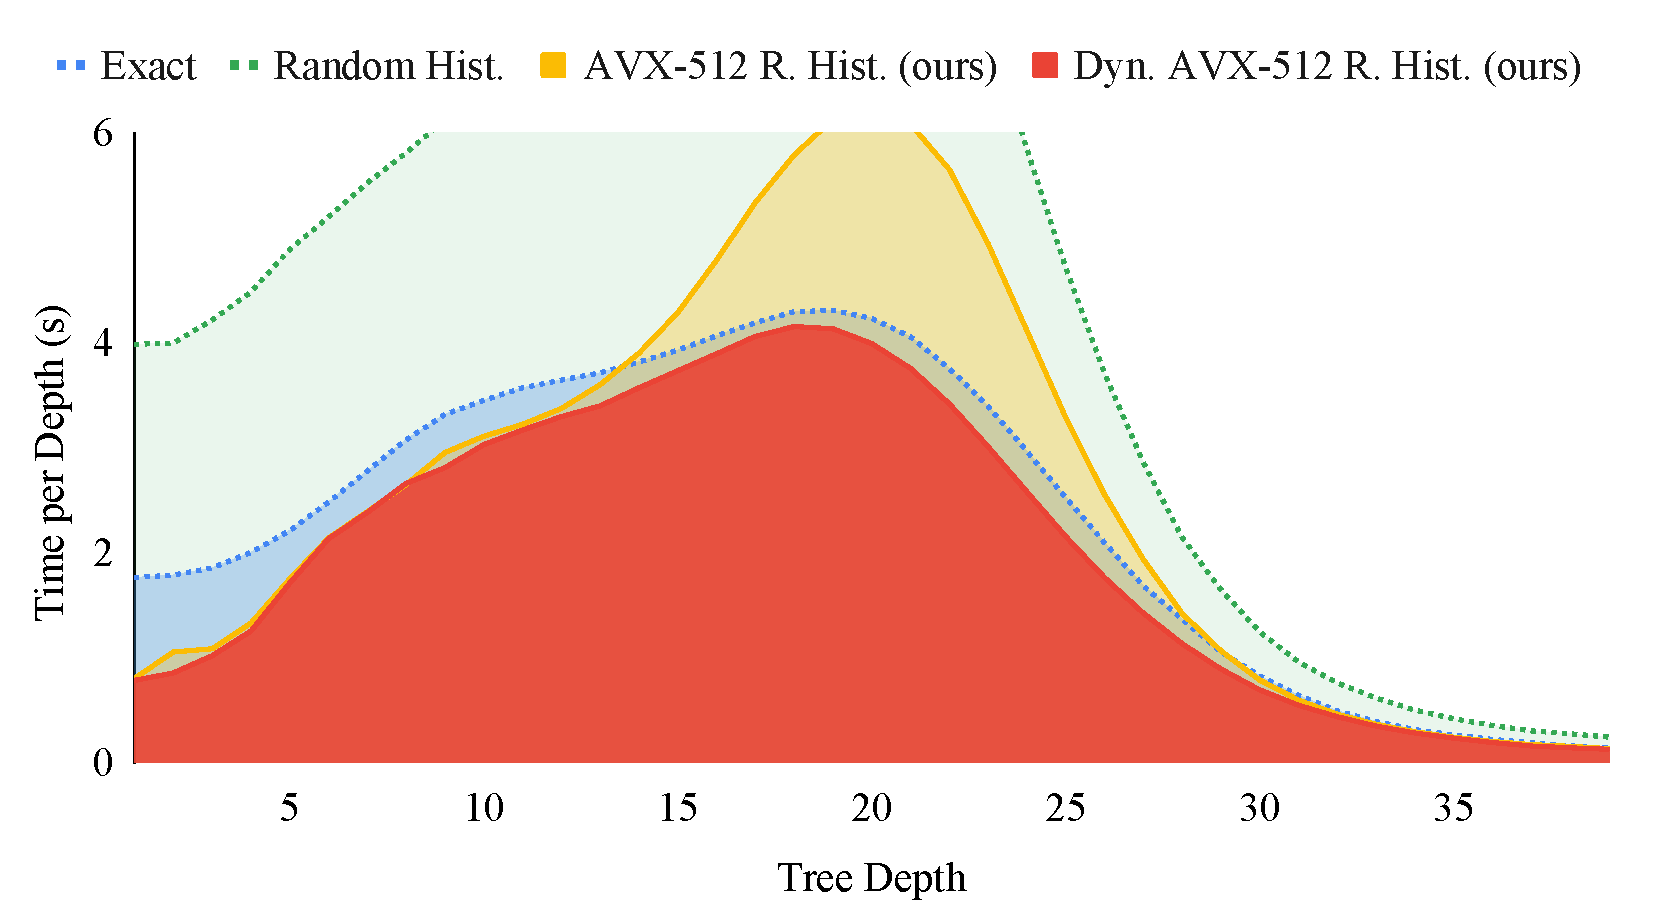
\includegraphics[width=\linewidth]{figures/intro/dynamic/Youtube-8m-spogbt-NodeTrain.pdf}
  \caption{SPO-GBT}
  \label{fig:motivation-nodetrain-gbt}
\end{subfigure}
\hfill
\begin{subfigure}[b]{0.32\textwidth}
  \centering
  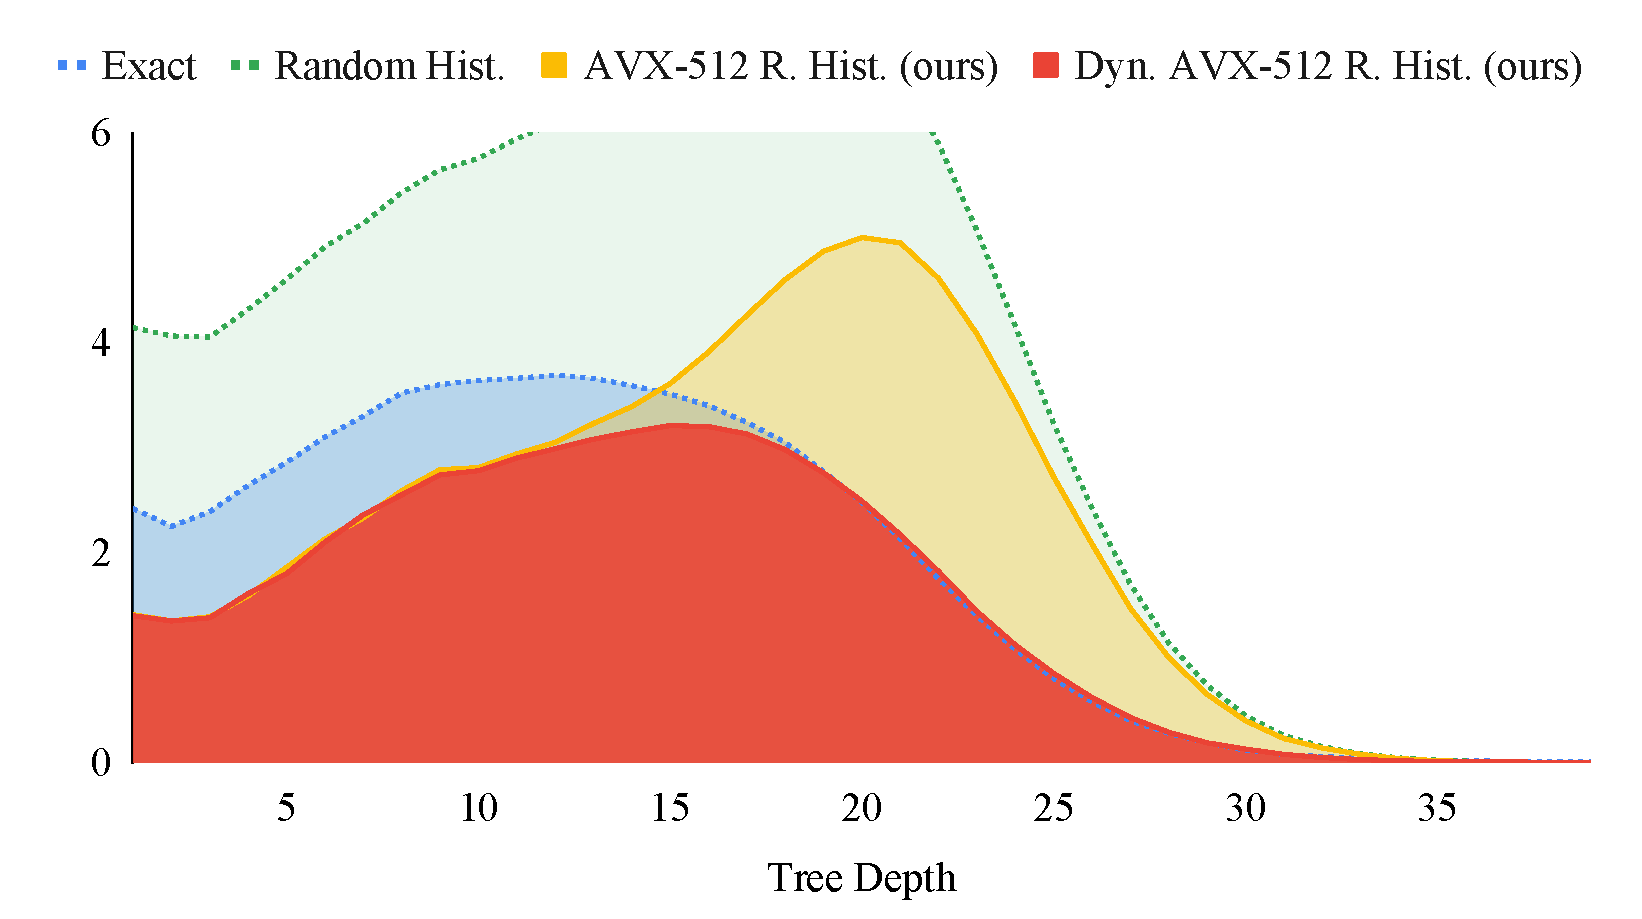
\includegraphics[width=\linewidth]{figures/intro/dynamic/Youtube-8m-sporf-NodeTrain.pdf}
  \caption{SPO-RF}
  \label{fig:motivation-nodetrain-rf}
\end{subfigure}
\hfill
\begin{subfigure}[b]{0.32\textwidth}
  \centering
  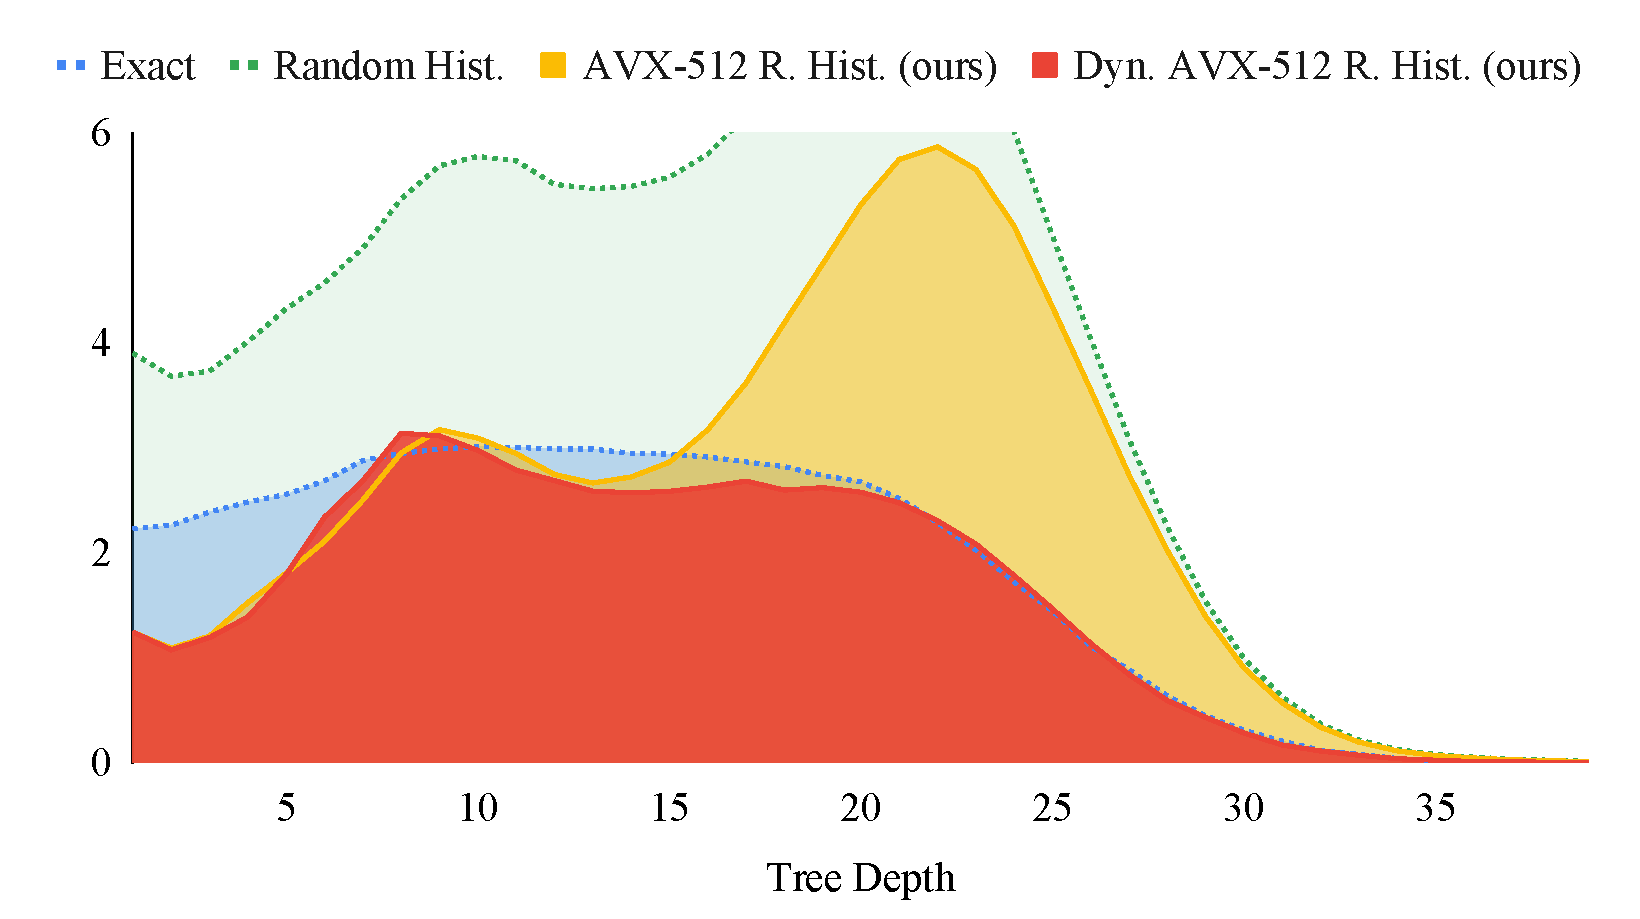
\includegraphics[width=\linewidth]{figures/intro/dynamic/Youtube-8m-aa-NodeTrain.pdf}
  \caption{AA-RF}
  \label{fig:motivation-nodetrain-aarf}
\end{subfigure}
\caption{Training time by tree depth on YouTube-8M, one panel per model family: SPO-GBT, SPO-RF and axis-aligned RF (AA-RF). Each panel compares the existing Exact and Random Histogram (256-bins) splitting with our Vectorized and Dynamic-Vectorized (256-bin) methods.}
\Description{Three line charts of \texttt{NodeTrain} time, one per model family, plotting per-depth training time against tree depth for four splitting methods.}
\label{fig:dynamic-motivation-nodetrain}
\end{figure*}

Training time not only depends on tree depth, but is skewed to shallower or deeper levels depending on the splitting method:  very large nodes near the root disproportionately affect the $O(n\log n)$ sorting cost, while large numbers of small nodes punish the $O(k)$ startup cost in histogram's $O(n\log k + k)$ complexity. GBTs are trained to depth 6, often to leverage a fast inference engine, such as QuickScorer~\cite{lucchese_quickscorer_2015}, which has a limit on maximum number of nodes. Training to depth 16-24 is common for Random Forests, and training to purity (full depth) is useful for posterior estimates~\cite{might1,might2}. The two families thus stress opposite ends of the depth range, and we contribute one optimization for each. Based on this observation, we contribute:

\emph{\textbf{(1) Vectorization of histogram construction}}. Histogram construction is asymptotically more efficient than sorting and should be faster when there are a sufficient number of samples. Yet with the powerful Highway sort replacing \texttt{std::sort}, the baseline histogram implementation using \texttt{std::upper\_bound()} is much slower than vectorized Highway sort (Figure~\ref{fig:dynamic-motivation-nodetrain}). We propose a hierarchical vectorized histogram filling implementation that leverages AVX2 and AVX-512, and delivers up to $2\times$ speedup over the SPO-RF Exact and $1.6\times$ over SPO-GBT, and beats scalar Random Hist. at all tree levels, while being mathematically identical.

\emph{\textbf{(2) Runtime-adaptive histograms.}} In deeper trees, the number of active nodes grows near-exponentially, and peaks at around halfway to purity. Though these nodes have few samples in them, histogram approaches must still pay the $O(k)$ startup cost of bin generation and scanning that Exact avoids (Fig.~\ref{fig:dynamic-motivation-nodetrain}). We propose a Dynamic switching method that adaptively chooses between vectorized histograms and exact splits depending on the number of samples at each node, with no detectable effect on accuracy (Table~\ref{tab:accuracy-rf}). This achieves up to 1.6$\times$ speedup when training deeper trees, bringing SPO performance on par with Axis-Aligned in YDF (Table~\ref{tab:train-time-vs-libraries}).

Neither optimization is tied to a depth or a model family. Vectorized filling accelerates every histogram split, and the dynamic switch acts on node size rather than depth, so both apply to GBT and RF alike, and to axis-aligned splits whenever features are not pre-sorted (Figure~\ref{fig:dynamic-motivation-nodetrain}(c)). At depth 6 over millions of rows no node is small enough to switch, so dynamic selection reduces to vectorized histograms, and at purity, all nodes switch. We therefore report each family in the setting it is used in practice, GBT at depth 6 and RF from depth 16 to purity. We provide extensive results on a variety of both natural and synthetic datasets (Table ~\ref{tab:all-datasets}), we sweep the full depth range in Table~\ref{tab:train-time-by-depth}. In addition, we provide a heatmap of predicted speedups by dataset size based on our evaluation (Figure~\ref{fig:speedup-heatmap}). An open-source implementation is available at (anonymized).

% \TODO{treat runtime comparison agianst XGboost and Catboost as apples-to-oranges}

% \TODO{include natural results table in main text (that supports numbers above). they're in Appendix}

%TODO RB Exact is a bad name for the baseline.

% only show three lines Exact, Random Hist and AVX-512.  Maybe rename Exact baseline?  Show results to level 8. State in caption that default for all major packages are 6 (XGBoost, CatBoost, LightGBM).


%and adopting vectorized sorting~\cite{}
%when building. This raiseed the baseline of for this paper by a factor of 2x-5x training time for larger datasets. 
%The first was the construction of linear combinations, which is a vector sum of a sparese scan

%Para 3: nature of SO methods.
%they create a tradeoff.  no class/regression inference time penalty. better accuracy and more robust. downside has been training time


% \{[Low priority] GBT and RF have similar computational properties. They only differ in parallelization. GBT has enough work up to depth 6 to keep CPU busy}

\section{Related Work}

% Para 1 -- oblique trees. Point: the split feature is synthesized at the node.
Oblique decision trees split on linear combinations of features rather than on a single feature. Breiman's original random forest paper proposed Forest-RC, which draws random linear combinations of a few inputs at each node~\cite{breiman}. OC1 searches for hyperplanes by hill climbing with random perturbations~\cite{murthy1994system}, canonical correlation forests derive the projection at each node from CCA~\cite{rainforth2015canonical}, and TAO learns sparse oblique trees by alternating optimization over the node hyperplanes~\cite{carreira2018alternating}, with bivariate trees as the two-feature special case~\cite{kairgeldin_bivariate_2024}. Sparse projection oblique random forests (SPO-RF)~\cite{tomita2020sparse} sample sparse random projections at each node and are implemented in treeple~\cite{treeple} and in YDF~\cite{ydf}, whose sparse oblique splits we optimize. SPO-RF is also the base learner of MIGHT, which trains forests to purity to obtain calibrated posteriors for biomedical screening~\cite{might1,might2}. Common to all of these methods is the fact that the feature being split exists only once the node's projection has been drawn and therefore cannot be presorted/pre-quantized before training.

% Para 2 -- how axis-aligned libraries find splits, and why none of it transfers. Merges the old presort and GPU paragraphs.
Axis-aligned learners find splits either exactly or with histograms. Exact splitting sorts the candidate feature's values within the node or scans a pre-sorted index of the whole column: ranger~\cite{wright2017ranger}, XGBoost's exact method~\cite{chen2016xgboost} and YDF~\cite{ydf} pre-sort, and scikit-learn's forests sort in the node~\cite{pedregosa2011scikit}. Histogram splitting, the default in LightGBM~\cite{ke2017lightgbm}, CatBoost~\cite{prokhorenkova2018catboost}, XGBoost's histogram method~\cite{chen2016xgboost}, TF Boosted Trees~\cite{ponomareva2017tf} and Spark MLlib~\cite{meng2016mllib}, quantizes every feature once before training into a fixed number of bins, so that filling a node's histogram is a scatter-add over stored bin indices with no search in the loop. XGBoost's local proposal variant~\cite{chen2016xgboost} and YDF's histogram splits~\cite{ydf} instead recompute bin boundaries per node, from the node's quantiles, its value range, or at random. Further savings come from sharing work across nodes: histogram subtraction derives one child's histogram from the parent's~\cite{ke2017lightgbm}, CatBoost's oblivious trees split every node of a level on the same feature and bin grid~\cite{prokhorenkova2018catboost}, and GPU trainers assemble partial histograms per thread block~\cite{wenthundergbm19,xu2025scalagbm}. 

% Para 4 -- SIMD bin lookup is known (PANDA, DB range partitioning); state exactly what is ours.
% Para 4 -- SIMD bin lookup is known; state exactly what is ours.
Resolving a key against a register of boundaries with one compare and a population count is established: per tree level in $k$-ary search~\cite{schlegel2009k} and in cache-resident range indexes~\cite{polychroniou_comprehensive_2014}, and in PANDA as a two-level SIMD scan over histogram boundaries~\cite{patwary_panda_2016}. All three build their boundaries once, then bin everything against them. Sparse oblique splits draw new boundaries for every projection at every node, so the structure is rebuilt per histogram and may serve only a few hundred lookups. Our lookup is sized for this: $B = W^2$ bins, two compare-and-count steps, one extra register, and an index, mathematically identical to \texttt{std::upper\_bound} (Section~\ref{v2:method:vectorization}).

% Para 3 -- per-node algorithm selection: precedent and the sharpened novelty claim.
To our knowledge, no tree learner switches between exact and histogram splitting per node, which is the choice our dynamic histograms make.

% Para 5 -- Highway. Library facts only; the 2-3x number lives in the appendix table.
Highway~\cite{wassenberg_vectorized_2022} is a C++ library of portable SIMD operations with runtime dispatch across x86, ARM and RISC-V targets. Its vectorized quicksort, VQSort, is the sort behind YDF's exact splits and the baseline for every speedup in this paper.

% Para 6 -- inference-side work, one sentence.
Inference performance optimization of RF and GBT includes: trees being compiled into C++~\cite{cho2018treelite,rapids} to improve memory layout and reduce branching and into tensor operations~\cite{nakandala2020tensor}. Cache-efficient memory layouts have been applied to nodes in multiple trees to reduce random I/O~\cite{browne2022forestpacking,madhyastha2021blockset}.

\section{Method}
\label{v2:method}

We describe the per-node computation of sparse oblique splitting and its cost, then the two optimizations: a vectorized bin lookup (Section~\ref{v2:method:vectorization}) and a per-node choice between histogram and exact splitting (Section~\ref{v2:method:dynamic}). Throughout, $n$ is the number of active samples at a node, $d$ the number of features, $P$ the projections per node, $k$ the histogram bins and $w$ the lanes of a vector register.

\subsection{Sparse Oblique Workflow and Its Cost}
\label{v2:method:workflow}

\begin{figure*}[thbp]
    \centering
    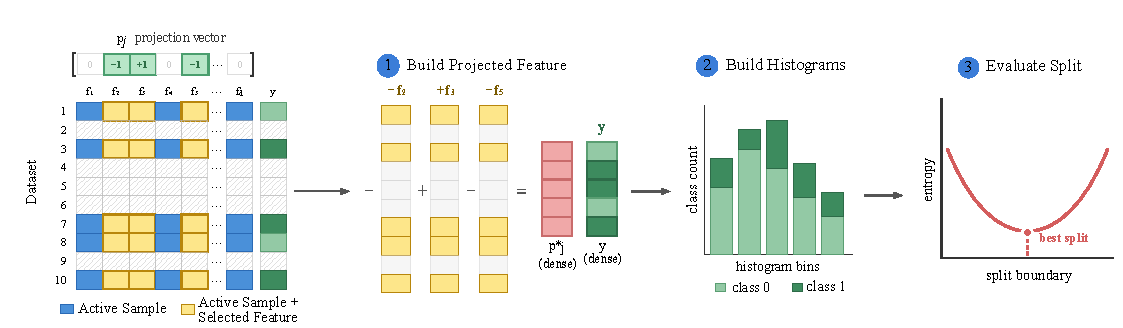
\includegraphics[width=1\linewidth]{figures/method/double_sparsity_illustration.pdf}

    \caption{Workflow at each tree node. Histogram splitting of a random linear combination of features requires sparse access in both rows and columns, computing a vector sum, building histograms and evaluating split boundaries.}
    \Description{Computation performed at each tree node includes: Sampling a projection, applying that projection, which involves sparse access across both rows and columns, building histograms and evaluating splits.}
    \label{fig:computenode}
\end{figure*}

YDF stores the data column by column and never copies it; a node is a sorted list of row indices, and each split partitions the parent's list in place. For RF the root holds a bootstrap sample of $n$ rows drawn with replacement, about 63\% of them distinct. At each node SPO draws $P=\lceil\sqrt{d}\,\rceil$ projections, capped at 1000~\cite{tomita2020sparse}, each a sparse vector with Binomial$(d,\,1.5/d)$ non-zeros, i.e.\ 1.5 on average, features chosen without replacement and weights uniform in $[-1,1]$. Every projection passes through four stages (Figure~\ref{fig:computenode}):
\begin{enumerate}
\item \emph{Sample Projection}: draw the non-zero features and weights.
\item \emph{Build Projected Feature}: gather the selected columns at the active rows and accumulate the weighted sum into $n$ values. Sparse in both dimensions and increasingly scattered with depth.
\item \emph{Build Histograms}, or sort: bin each value and count its class, or sort the values for exact splitting.
\item \emph{Evaluate Split}: score every candidate threshold by information gain. Keep the best over all $P$ projections.
\end{enumerate}

\emph{Exact} splitting packs each (value, label) pair into a 64-bit key, sorts the $n$ keys with Highway's VQSort~\cite{wassenberg_vectorized_2022} and scans them once, considering the midpoint between every pair of adjacent distinct values: $O(n\log n)$ per projection. \emph{Random Histogram} splitting draws $k$ thresholds uniformly between the node's minimum and maximum value, sorts them, bins each value by binary search over the thresholds, and scans the $k$ candidates: $O(n\log k)$ for the lookups plus an $O(k)$ term independent of $n$ for drawing and sorting the thresholds, initializing the counters and scanning the bins. Because the thresholds are random rather than equally spaced, the bin index has no closed form, unlike learners that quantize each feature once before training~\cite{ke2017lightgbm,prokhorenkova2018catboost}. The search runs once per value, per projection, per node.

Figure~\ref{fig:decompose}, from our per-node timers, breaks Random Histogram training time down by stage and depth on 1M rows and 4096 features. % this is for scalar, but vectorized looks identical, except Build Histogram section is bigger
Building histograms dominates at every depth. Its cost per depth is flat while nodes are large, since each depth bins all $n$ samples once per projection, and grows from depth 10 on, where the number of nodes doubles per level and the $O(k)$ work per projection grows with it. Evaluate Split, also $O(k)$ per projection, appears at the same depth. The two optimizations follow: in shallow trees the per-value lookup dominates, in deep trees the per-projection fixed cost does.

\begin{figure}[t]
    \centering
    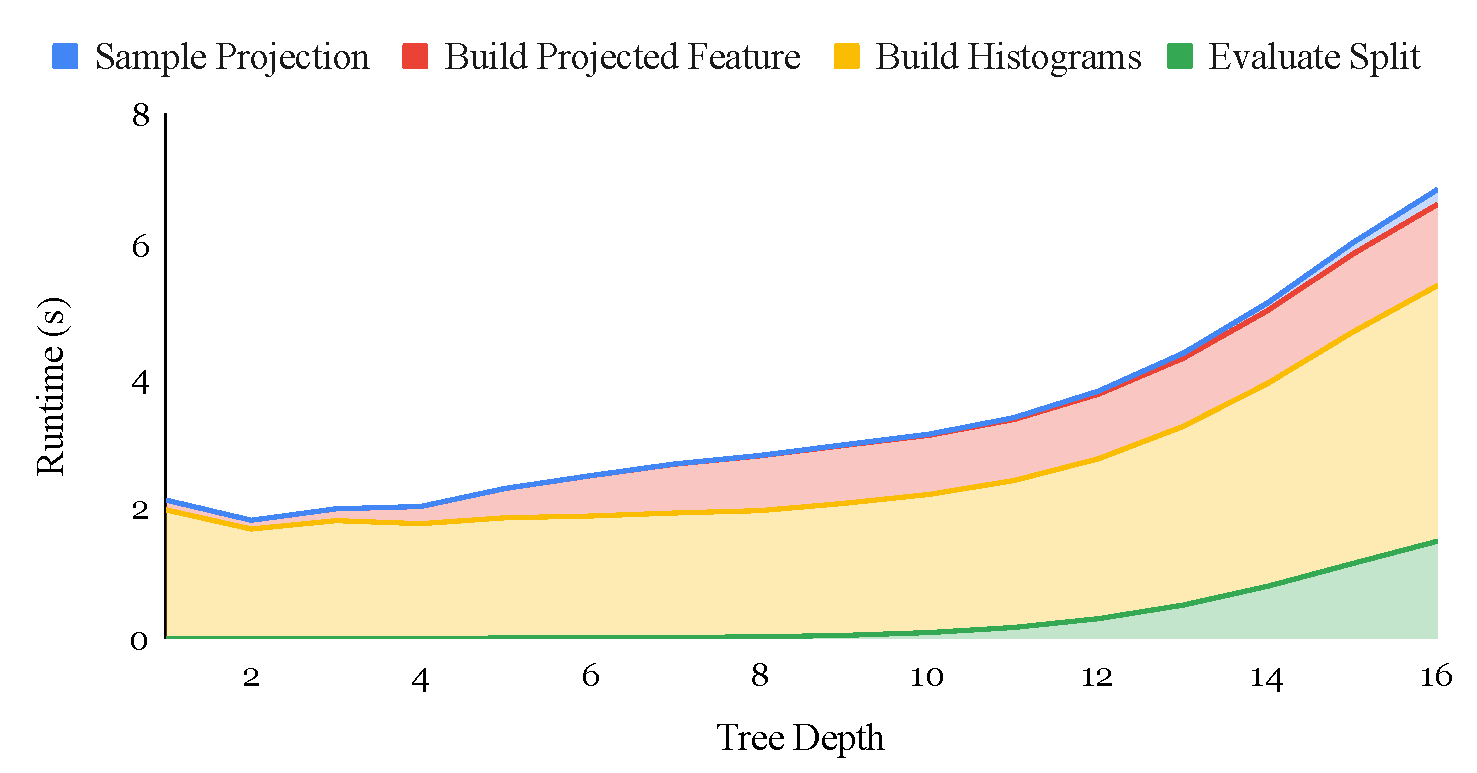
\includegraphics[width=\linewidth]{figures/results/proportion_of_histogram_time.pdf}
    \caption{Comparative runtime of the different components of computation for histogram splitting. The dataset has 1M samples and 4096 features.}
    \Description{Share of histogram runtime (in dynamic mode) attributable to each of 4 subfunctions. Plot reveals Build Histograms requires the majority of the time, necessitating Vectorization. }
    \label{fig:decompose}
\end{figure}

\subsection{Vectorization of Histogram Filling}
\label{v2:method:vectorization}

\begin{figure*}[!t]
\centering
\begin{subfigure}[b]{0.44\textwidth}
\centering
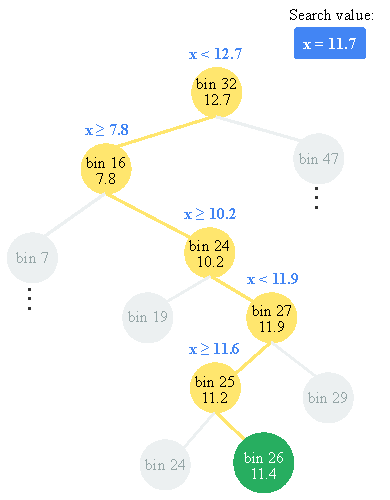
\includegraphics[width=.8\linewidth]{figures/method/vectorization/binary_search_illustration.pdf}
% \caption{Illustration of Binary Search on 64 histogram bins.}
\end{subfigure}
\begin{subfigure}[b]{0.54\textwidth}
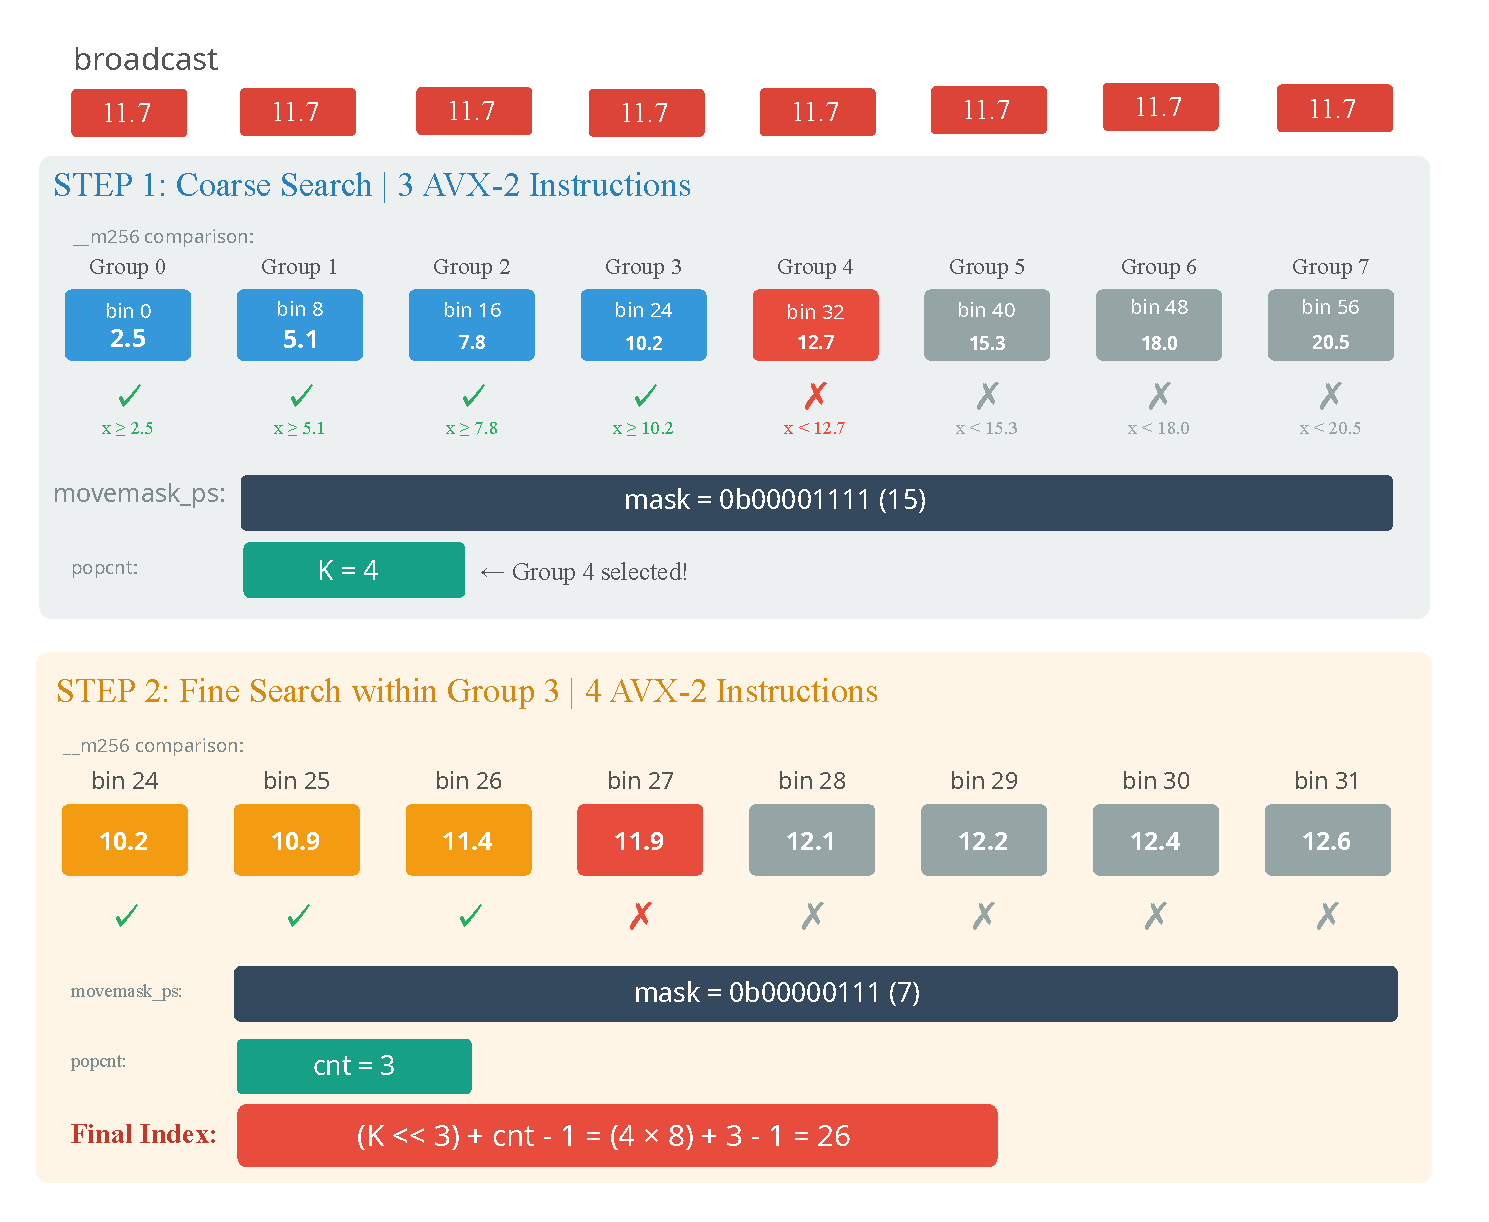
\includegraphics[width=\linewidth]{figures/method/vectorization/vectorized_binary_search_illustration.pdf}
% \caption{Illustration of conversion of Binary Search into AVX2 SIMD instructions.}
\end{subfigure}
\caption{Mapping sample points to histograms using binary search (left) and our vectorized AVX2 implementation (right).}
\label{fig:vectorization-illustration}
\Description{Illustration of mapping sample points to histograms using binary search (default, left) and our vectorized implementation (right).}
\end{figure*}

YDF bins a value with \texttt{std::upper\_bound}, a binary search over the $k$ sorted thresholds (Figure~\ref{fig:vectorization-illustration}, left): $\log_2 k$ dependent steps, each ending in a data-dependent branch that can cause mispredictions. A linear scan avoids the branches but costs $k$ comparisons per value.

We replace the search by two levels of SIMD comparisons (Figure~\ref{fig:vectorization-illustration} right). With $w$ lanes, $w=8$ for AVX2 and $w=16$ for AVX-512, we use $k=w^2$ bins. Once per histogram we copy the sorted thresholds $T[0,k)$ into an aligned array and build a coarse table $C[0,w)$ of the last threshold of each group of $w$ bins, $C[g]=T[w(g+1)-1]$. Per value $x$, one broadcast, one compare against $C$ and one \texttt{popcnt} give $K$, the number of groups whose thresholds are all at most $x$, i.e.\ the group containing $x$; a second compare against the $w$ thresholds of group $K$ and a second \texttt{popcnt} give the count $j$ of thresholds at most $x$ within it, and the bin is $wK+j-1$, or $-1$ if $x$ lies below every threshold. If $K=w$ the value belongs to the last bin.

% \begin{figure}[t]
% \begin{lstlisting}[basicstyle=\ttfamily\footnotesize, columns=fullflexible, keepspaces=true, morecomment={[l]{//}}, commentstyle=\itshape]
% // Setup, once per histogram (T[0..k) sorted, k = w*w)
% for g in 0..w-1: C[g] = T[w*(g+1) - 1]  // last of group g

% // Lookup per value x: largest threshold <= x, or -1
% vx = broadcast(x)
% K  = popcnt(mask(vx >= C[0..w)))        // group of x
% if K == w: return k - 1                 // above all
% j  = popcnt(mask(vx >= T[w*K .. w*K+w)))  // in group K
% return w*K + j - 1
% \end{lstlisting}
% \caption{Two-level SIMD bin lookup. One vector compare and popcount select the group of $w$ bins, a second pair selects the bin. $w=8$ on AVX2 (64 bins) and $w=16$ on AVX-512 (256 bins).}
% \Description{Pseudocode of the two-level SIMD bin lookup.}
% \label{v2:lst:binsearch}
% \end{figure}

The lookup is seven vector and bit-count instructions on AVX2 and five on AVX-512, whose compares write a mask register directly, with no data-dependent branch. Thresholds are drawn, sorted and used exactly as before, and the lookup returns the same index as \texttt{std::upper\_bound} for every input, which debug builds assert, so the trees are bit-identical to the scalar implementation. The kernel is selected at run time from the CPU and the bin count, with a scalar fallback, and serves the axis-aligned histogram finder unchanged. The two widths are not interchangeable: the lookup costs the same, but the $O(k)$ per-projection work is four times larger with 256 bins, so AVX-512 wins only where $n$ is large relative to $k$ and loses in deep trees (Figure~\ref{fig:AVX-512-slower}).

\subsection{Dynamic Histogramming}
\label{v2:method:dynamic}

\begin{figure}[h!]
    \centering
    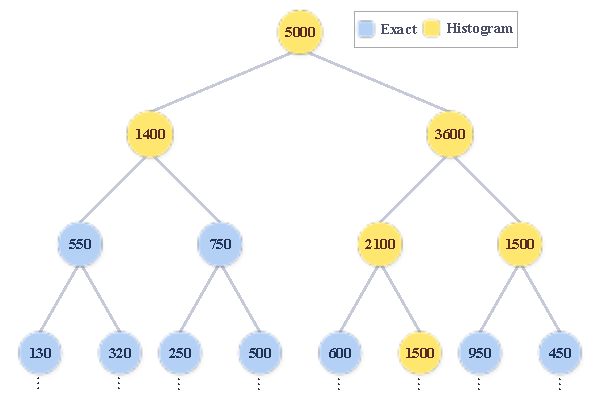
\includegraphics[width=1\linewidth]{figures/method/dynamic_histogram/dynamic_histogram_tree_illustration.pdf}
    \caption{Illustration of the selection of exact splitting and histogram splitting as a function of the number of active samples in a tree node with a breakeven point of 1300.}
    \Description{Illustration of the selection of exact splitting and histogram splitting in an example decision tree.}
    \label{fig:levels}
\end{figure}

Histogram and exact splitting are expensive at opposite ends of the tree (Figure~\ref{fig:dynamic-motivation-nodetrain}). Near the root the $O(n\log n)$ sort dominates and histograms are faster~\cite{ydf,prokhorenkova2018catboost}, and deep in the tree the number of nodes doubles per level while samples per node halve, and the $O(k)$ work per histogram, paid at every node regardless of $n$, dominates.

We therefore choose the finder per node: before the projection loop, a node with $n<\tau$ samples uses exact splitting for all its projections, otherwise vectorized histograms. The choice costs one comparison per node, and nodes at the same depth may have differerent split types (Figure~\ref{fig:levels}). The threshold $\tau$ is a single integer hyperparameter that depends on the kernel and the sort, not on the dataset. We provide a microbenchmark to heuristically set it at the first run on a new machine. For our test, we chose $\tau=250$ for the 64-bin AVX2 kernel and $1000$ for the 256-bin AVX-512 kernel. A full runtime comparison of various thresholds is provided in Figure~\ref{fig:threshold-sensitivity}. Near the top of the tree, most nodes clear the threshold and dynamic splitting chooses as vectorized histograms, whereas below it a growing share of nodes is exact, avoiding the histogram's fixed cost.

Dynamic forests are not node-for-node identical to histogram forests: exact splitting considers every midpoint instead of $k$ random thresholds, and since the histogram finder consumes random numbers for its thresholds and the exact finder does not, projections drawn after the first switch differ as well. The split rule is unchanged at every node with $n\ge\tau$, and we find no detectable effect on accuracy (Table~\ref{tab:accuracy-rf}).

% Both optimizations also apply to axis-aligned splits whenever features are not pre-sorted, as the AA-RF panel of Figure~\ref{fig:dynamic-motivation-nodetrain} shows.

%Explain that there are an increasing number of nodes with increasing levels.  So split evaluation and build project feature scale with the number of nodes and have increasing cost at depth.

%Make it clear that this is pre-vectorization.

% \textcolor{red}{Finish subsection with breakdown of runtime by function (interpret fig. 3).}

% Our measurements show that histogram construction dominates the runtime cost of training. Note that is comprises 87\% below level 6 (default depth for YDF GBT, XGBoost and Catboost). 

% AL: should have included figure showing reduction

% Para: Describe algorithms with pseudocode and figure 6.

% Para: Properties -- # instructions, no branches, branch miss rate of std:upper.



% Para: relative merits of 64 abd 512.
% We present results for both AVX2 and AVX-512 methods in section~\ref{sec:results}. We must note that while the vector-compare part takes the same amount of time between our AVX2 and AVX-512 methods, their runtime is nonetheless dissimilar. This is caused by AVX-512's 256-bins requiring 4x more work to be sampled at setup, then scanned at teardown. This is an unavoidable linear cost in the number of bins.

% % \TODO{pseudocode} 

% We also provide a 64 bin, 8-bit wide AVX2 implementation. Figure~\ref{fig:vectorization-illustration} compares the AVX-implementation with binary search over 64 bins. The binary search uses 7 instructions with one branch per node for a minimum of 42 serial instructions and not branch prediction-friendly. Miss rate of the binary search depends on the skewness of the child nodes: skewed subtrees have higher prediction, while even splits approach ~50\% miss rate. AVX2 broadcasts the search value to a vector. Does a parallel compare and resolves the coarse grained bin using a mask and count intrinsic. It repeats this at a finer grain for a total of 16 instructions.



% \subsection{Dynamic Histogramming}

% \textit{\textbf{Applies on Axis-aligned RF too} (if no PRESORT)} %. Not GBTs tho bcs. they use depth 6-8

% Figure~\ref{fig:dynamic-motivation} reveals histograms for approximate splitting and sorting for exact splitting have different costs at different levels in the tree. Conventional wisdom is that histograms are faster, require less memory, and perform favorable sequential memory access~\cite{ydf,prokhorenkova2018catboost}.
% While this is true for nodes higher in the tree with many active samples--the $O(n\log n)$ complexity of sorting dominates the $O(k+n\log k)$ cost of filling a $k$-bin histogram--down the tree, when the number of active samples in each node becomes small and the number of nodes grows large, the fixed cost of allocating and initializing histograms dominates. This leads to the core idea of using histograms for high cardinality nodes and sorting for low cardinality nodes. The resulting dynamic histograms track the best performance of both splitting methods. Although adaptively switching between the two techniques changes the algorithm, we reveal only minor variances in accuracy from either splitting technique.

% The exact cardinality varies depending on the system architecture. We determine the crossover value using a simple microbenchmark that runs one time at the start of training. It applies to all nodes of all trees.

% Our study revealed performance concerns when training SO-YDF trees to purity. When the number of active samples is small, histogram construction dominates runtime. There are fixed costs to set up a histogram and these are incurred at each node. Referring back to Figure \ref{fig:dynamic-motivation}, histograms operate relatively much faster at the top levels of the tree when the number of samples are large. These benefits endure through the first 12-13 levels of the tree on a 1M-row balanced dataset. Below this level, there are many active nodes, each of which requires a histogram. Here, sorting few samples can be much faster than building a histogram. %Implementations of {\sf std::sort()} have many optimizations to sort few elements, including unguarded insertions.

% The  breakeven point depends on the number of active samples and the  hardware. Tree depth is just our proxy for visualizing the total runtime. Figure \ref{fig:threshold-sensitivity} show the relative cost of exact splits versus histograms on server CPU, showing a breakeven point of just over 1200 points. 
% % We also include the GPU results that show when it is beneficial to offload a computation to a GPU when available. 
% The break-even point is determined by a microbenchmark that runs at the start of training. This takes less than 100ms to perform a binary search over reasonable parameters.

% % Our results will show that perforamnce is robust over a range on this parameter, i.e. not hard to tune.  

% During tree-construction, we dynamically choose between a histogram and sorting on a node-by-node basis. Two nodes at the same tree depth may use different techniques (Figure \ref{fig:levels}). From a performance standpoint, this solves the problem with creating deep trees.  We avoid the overhead of sorting at high cardinality nodes and of histograms for low cardinality nodes. There is only a small performance penalty for training to purity.  Nodes beyond depth 20 use less 5\% of the runtime (Figure \ref{fig:threshold-sensitivity}).


%  %The exact breakeven point depends on the functions being compared and the underlying hardware\footnote{The exact breakeven point depends on the underlying hardware. We provide code to find this breakeven point. In this test,  64 bin histograms were used.}. We experiment to find the inflection point (Figure \ref{fig:threshold-sensitivity}), revealing it to be $\sim 350$ for Random Histograms and $\sim 200$ for Vectorized Random histograms, due to the latter being faster.

% Dynamic histograms produce different trees and potentially different learning outcomes. The resulting forests are most similar to those constructed by histograms. The high levels of the trees are the same. They differ only in the low cardinality nodes when exact splitting chooses a boundary that separates elements that are in the same bucket. The accuracy of all methods; histograms, exact, and dynamic, are statistically indistinguishable.




\section{Results}
\label{sec:results}

% v2 (2026-09-26): Results rewritten to follow the abstract/intro claims. New text sits
% above the previous text of each subsection, kept verbatim below a 'previous text' marker.

We report each contribution in the setting described in the introduction. Section~\ref{app:parameters} sets the protocol and the baseline. Section~\ref{sec:res-depth6} measures vectorized histogram filling on depth-6 trees, for SPO-GBT and SPO-RF. Section~\ref{sec:res-depth16} follows SPO-RF from depth 16 to 24, where the dynamic switch takes over from vectorization, and Section~\ref{sec:res-purity} completes the depth range at purity and compares against YDF's axis-aligned RF. Section~\ref{sec:res-scalability} maps the speedup over rows and features, Section~\ref{sec:dyn} separates the two optimizations and the two bin counts, Section~\ref{app:threshold-sensitivity} varies the switch threshold, and Section~\ref{sec:res-accuracy} shows that this does not change accuracy. Table~\ref{tab:train-time-by-depth} (SPO-RF, six depths) and Table~\ref{tab:train-time-gbt-depth6} (SPO-GBT, depth 6) in the appendix hold the full timing results.

\subsection{Experimental Setup}
\label{app:parameters}

\begin{table}[]
    \centering
    \begin{tabular}{c|c|c|c}
Dataset & Task & Rows & Feat. \\
\midrule
HIGGS~\cite{higgs_280} & bin & 11,000,000 & 28 \\
SUSY~\cite{susy_279} & bin & 5,000,000 & 18 \\
Epsilon~\cite{chang2011libsvm} & bin & 400,000 & 2,000 \\
YouTube-8M~\cite{abu2016youtube}         & mul$^*$   & 3,888,919            & 1152 \\
Shifts Weather~\cite{malinin2021shifts}   & reg$^*$   & 3,129,592            & 127 \\
ClimSim~\cite{yu2023climsim}              & reg$^*$   & 10,091,520           & 124 \\
Jane Street~\cite{jane-street-real-time-market-data-forecasting}       & reg$^*$   & 10,213,190$^\dagger$ & 82
\end{tabular}
\caption{Natural Datasets used in our experiments. * - treated as \texttt{bin}. $\dagger$ - subset used. Full datasets and their description in Table~\ref{tab:all-datasets}.}
\label{tab:natural-datasets}
\end{table}

\paragraph{Hardware and software} All timings come from one AWS m7i.metal-24xl instance (Intel Xeon Platinum 8488C, 48 physical cores, 384\,GiB, Ubuntu 24.04) running YDF compiled with Intel ICX 2025.2.1 and AVX-512 enabled, with 48 threads. Random forests train one tree per thread; gradient-boosted trees parallelize the split search within each tree. Times cover training only: dataset loading and model serialization are excluded.

\paragraph{Learners} SPO-RF: 240 trees, bootstrap sampling with replacement and a bag size equal to the number of rows, \code{min\_examples}=1, maximum depth 6, 10, 16, 20, 24 or unlimited (purity). SPO-GBT: 300 trees of depth 6, shrinkage 0.1, \code{min\_examples}=5. Every node samples $\lceil\sqrt{F}\rceil$ sparse projections (at most 1000) with 1.5 expected non-zero features each. YDF defaults apply elsewhere.

\paragraph{Split finders and baseline} Exact splits sort the projected values with Highway VQSort and are the baseline for every speedup below: speedup $= T_{\mathrm{Exact}}/T_{\mathrm{method}}$, so values above 1 are faster. Table~\ref{tab:stdsort-vs-highway} in the appendix relates this baseline to the \texttt{std::sort} exact finder of the released YDF, which it improves by 1.8--3.5$\times$. Random histograms draw their bin boundaries per projection and use 64 bins with the scalar (\texttt{std::upper\_bound}) and AVX2 binners and 256 bins with the scalar and AVX-512 binners. The dynamic variants bin nodes with at least $\tau$ rows and sort the rest, with $\tau=250$ for AVX2/64 bins and $\tau=1000$ for AVX-512/256 bins (Section~\ref{app:threshold-sensitivity}). The scalar 64-bin binner has a breakeven threshold $\tau>50000$, and therefore appears only as an non-Dynamic baseline.

\paragraph{Datasets and protocol} Sevel natural datasets (Table~\ref{tab:natural-datasets}) and 13 Trunk shapes spanning 15k to 4.5M rows and 32 to 1.6M features (Table~\ref{tab:train-time-by-depth}). Because regression is slightly slower than classification, regression targets are thresholded at the training-set median and the multi-label YouTube-8M target is its most frequent class against the rest. 
% Tables~\ref{tab:train-time-by-depth} and \ref{tab:train-time-gbt-depth6} and Figures~\ref{fig:overall} and \ref{fig:speedup-heatmap} are single runs per cell with one seed.
Accuracy protocols are stated in Section~\ref{sec:res-accuracy}.

% ---- previous text below (kept for comparison. v2 rewrite above, 2026-09-26) ----


% \textit{\textbf{Big embeddings are an important use case at Google. Google can't give access, but we make a proxy. }} The use of tabular-embedding multimodal is picking up pace. \textit{Text + LLM embeddings is a strong GBT use case. Tabular structure gives benefit \cite{jiang2026multimodal}}. Good but small: MulTABench \cite{arazi_multabench_2026}: Multimodal Tabular Benchmark - great but small: max 114,000 rows x 245 features, AutoML Bag of Tricks~\cite{tang_bag_2024} (20k rows), AutoGluon–TimeSeries~\cite{shchur_autogluon-timeseries_2023} (100k), Multimodal Tabular Reasoning~\cite{jiang2026multimodal}, however, these are too small for a performance study. As such, we use datasets described in~\ref{tab:natural-datasets}.


\subsection{Depth 6 - GBTs}
\label{sec:res-depth6}

% fig:overall lives in the generated file (make_e2e_grid_figure.py). caption/label are set there.
% Generated by benchmarks/src/utils/make_e2e_grid_figure.py -- do not hand-edit.
% Needs \usepackage{pgfplots}\pgfplotsset{compat=1.18}\usepgfplotslibrary{groupplots}.
\definecolor{e2ec0}{HTML}{4285F4}
\definecolor{e2ec1}{HTML}{34A853}
\definecolor{e2ec2}{HTML}{0B6B3A}
\definecolor{e2ec3}{HTML}{B57BFF}
\definecolor{e2ec4}{HTML}{6A1B9A}
\definecolor{e2ec5}{HTML}{FBBC04}
\definecolor{e2ec6}{HTML}{EA4335}
\pgfplotsset{bar0/.style={ybar, fill=e2ec0, draw=e2ec0!70!black, line width=0.2pt}}
\pgfplotsset{bar1/.style={ybar, fill=e2ec1, draw=e2ec1!70!black, line width=0.2pt}}
\pgfplotsset{bar2/.style={ybar, fill=e2ec2, draw=e2ec2!70!black, line width=0.2pt}}
\pgfplotsset{bar3/.style={ybar, fill=e2ec3, draw=e2ec3!70!black, line width=0.2pt}}
\pgfplotsset{bar4/.style={ybar, fill=e2ec4, draw=e2ec4!70!black, line width=0.2pt}}
\pgfplotsset{bar5/.style={ybar, fill=e2ec5, draw=e2ec5!70!black, line width=0.2pt}}
\pgfplotsset{bar6/.style={ybar, fill=e2ec6, draw=e2ec6!70!black, line width=0.2pt}}
\begin{figure*}[!t]
    \centering
    \begin{tikzpicture}
    \begin{groupplot}[
        group style={group size=2 by 2, horizontal sep=0.75cm, vertical sep=1.05cm,
            xticklabels at=edge bottom},
        width=0.53\textwidth, height=4.5cm,
        /pgf/bar width=0.1, ybar, ybar legend,
        xmin=0.45, xmax=7.55, ymin=0, ymax=1.5, ytick={0,0.5,1,1.5},
        xtick={1,2,3,4,5,6,7},
        xticklabels={Epsilon, Jane Street, SUSY, HIGGS, YouTube-8M, Trunk 150k$\times$4096, Trunk 15k$\times$400k},
        xticklabel style={rotate=28, anchor=north east, font=\scriptsize, yshift=-1pt},
        yticklabel style={font=\scriptsize}, title style={font=\small, yshift=-4pt},
        tick align=outside, tick pos=left, axis line style={black!50},
        legend columns=3, legend cell align=left,
        legend style={font=\scriptsize, draw=gray!40, /tikz/every even column/.append style={column sep=5pt}},
        legend image code/.code={\draw[#1] (0cm,-0.08cm) rectangle (0.25cm,0.14cm);},
    ]
    \nextgroupplot[title={SPO-GBT, depth 6}]
    \addplot[bar0, /pgf/bar shift=-0.3500] coordinates {(1,1.0000) (2,1.0000) (3,1.0000) (4,1.0000) (5,1.0000) (6,1.0000) (7,1.0000)};
    \addplot[bar1, /pgf/bar shift=-0.2500] coordinates {(1,1.5563) (2,1.0293) (3,1.4808) (4,1.5305) (5,0.9780) (6,1.2973) (7,1.7768)};
    \addplot[bar2, /pgf/bar shift=-0.1500] coordinates {(1,2.1522) (2,1.3991) (3,2.0342) (4,2.0756) (5,1.3292) (6,1.8327) (7,2.6210)};
    \addplot[bar3, /pgf/bar shift=0.0000] coordinates {(1,0.7031) (2,0.5444) (3,0.6787) (4,0.6907) (5,0.5574) (6,0.5327) (7,0.7466)};
    \addplot[bar4, /pgf/bar shift=0.1000] coordinates {(1,0.7808) (2,0.5531) (3,0.6502) (4,0.6743) (5,0.5867) (6,0.5790) (7,0.8466)};
    \draw[gray!70, dashed, line width=0.5pt] (axis cs:0.45,1) -- (axis cs:7.55,1);
    \draw[white, line width=1.1pt] (axis cs:0.6880,1.380) -- (axis cs:0.8120,1.430);
    \draw[white, line width=1.1pt] (axis cs:0.6880,1.440) -- (axis cs:0.8120,1.490);
    \draw[white, line width=1.1pt] (axis cs:3.6880,1.380) -- (axis cs:3.8120,1.430);
    \draw[white, line width=1.1pt] (axis cs:3.6880,1.440) -- (axis cs:3.8120,1.490);
    \draw[white, line width=1.1pt] (axis cs:6.6880,1.380) -- (axis cs:6.8120,1.430);
    \draw[white, line width=1.1pt] (axis cs:6.6880,1.440) -- (axis cs:6.8120,1.490);
    \draw[white, line width=1.1pt] (axis cs:0.7880,1.380) -- (axis cs:0.9120,1.430);
    \draw[white, line width=1.1pt] (axis cs:0.7880,1.440) -- (axis cs:0.9120,1.490);
    \draw[white, line width=1.1pt] (axis cs:2.7880,1.380) -- (axis cs:2.9120,1.430);
    \draw[white, line width=1.1pt] (axis cs:2.7880,1.440) -- (axis cs:2.9120,1.490);
    \draw[white, line width=1.1pt] (axis cs:3.7880,1.380) -- (axis cs:3.9120,1.430);
    \draw[white, line width=1.1pt] (axis cs:3.7880,1.440) -- (axis cs:3.9120,1.490);
    \draw[white, line width=1.1pt] (axis cs:5.7880,1.380) -- (axis cs:5.9120,1.430);
    \draw[white, line width=1.1pt] (axis cs:5.7880,1.440) -- (axis cs:5.9120,1.490);
    \draw[white, line width=1.1pt] (axis cs:6.7880,1.380) -- (axis cs:6.9120,1.430);
    \draw[white, line width=1.1pt] (axis cs:6.7880,1.440) -- (axis cs:6.9120,1.490);
    \nextgroupplot[title={SPO-RF, depth 10}]
    \addplot[bar0, /pgf/bar shift=-0.3500] coordinates {(1,1.0000) (2,1.0000) (3,1.0000) (4,1.0000) (5,1.0000) (6,1.0000) (7,1.0000)};
    \addplot[bar1, /pgf/bar shift=-0.2500] coordinates {(1,1.1974) (2,0.7162) (3,0.8726) (4,0.8126) (5,0.8985) (6,1.3052) (7,1.5191)};
    \addplot[bar2, /pgf/bar shift=-0.1500] coordinates {(1,1.5118) (2,0.8300) (3,1.0348) (4,0.9466) (5,1.0719) (6,1.6716) (7,2.0709)};
    \addplot[bar3, /pgf/bar shift=0.0000] coordinates {(1,0.7087) (2,0.5889) (3,0.6161) (4,0.6315) (5,0.6454) (6,0.7319) (7,0.8538)};
    \addplot[bar4, /pgf/bar shift=0.1000] coordinates {(1,0.7287) (2,0.5952) (3,0.6135) (4,0.6423) (5,0.6508) (6,0.7791) (7,1.0362)};
    \draw[gray!70, dashed, line width=0.5pt] (axis cs:0.45,1) -- (axis cs:7.55,1);
    \draw[white, line width=1.1pt] (axis cs:6.6880,1.380) -- (axis cs:6.8120,1.430);
    \draw[white, line width=1.1pt] (axis cs:6.6880,1.440) -- (axis cs:6.8120,1.490);
    \draw[white, line width=1.1pt] (axis cs:0.7880,1.380) -- (axis cs:0.9120,1.430);
    \draw[white, line width=1.1pt] (axis cs:0.7880,1.440) -- (axis cs:0.9120,1.490);
    \draw[white, line width=1.1pt] (axis cs:5.7880,1.380) -- (axis cs:5.9120,1.430);
    \draw[white, line width=1.1pt] (axis cs:5.7880,1.440) -- (axis cs:5.9120,1.490);
    \draw[white, line width=1.1pt] (axis cs:6.7880,1.380) -- (axis cs:6.9120,1.430);
    \draw[white, line width=1.1pt] (axis cs:6.7880,1.440) -- (axis cs:6.9120,1.490);
    \nextgroupplot[title={SPO-RF, depth 20}]
    \addplot[bar0, /pgf/bar shift=-0.3500] coordinates {(1,1.0000) (2,1.0000) (3,1.0000) (4,1.0000) (5,1.0000) (6,1.0000) (7,1.0000)};
    \addplot[bar1, /pgf/bar shift=-0.2500] coordinates {(1,1.4956) (2,0.9027) (3,1.0708) (4,1.0226) (5,1.0937) (6,1.6122) (7,1.5965)};
    \addplot[bar2, /pgf/bar shift=-0.1500] coordinates {(1,2.2918) (2,1.1026) (3,1.3608) (4,1.2535) (5,1.4051) (6,2.5911) (7,2.4816)};
    \addplot[bar3, /pgf/bar shift=0.0000] coordinates {(1,0.9799) (2,0.7138) (3,0.7102) (4,0.7413) (5,0.7445) (6,1.0528) (7,1.0762)};
    \addplot[bar4, /pgf/bar shift=0.1000] coordinates {(1,1.4981) (2,0.7422) (3,0.7666) (4,0.7809) (5,0.8331) (6,1.7200) (7,1.6647)};
    \addplot[bar5, /pgf/bar shift=0.2500] coordinates {(1,0.8266) (2,0.7047) (3,0.6938) (4,0.7338) (5,0.7324) (6,0.8489) (7,0.8732)};
    \addplot[bar6, /pgf/bar shift=0.3500] coordinates {(1,0.8608) (2,0.7139) (3,0.7028) (4,0.7425) (5,0.7399) (6,0.8892) (7,0.9006)};
    \draw[gray!70, dashed, line width=0.5pt] (axis cs:0.45,1) -- (axis cs:7.55,1);
    \draw[white, line width=1.1pt] (axis cs:5.6880,1.380) -- (axis cs:5.8120,1.430);
    \draw[white, line width=1.1pt] (axis cs:5.6880,1.440) -- (axis cs:5.8120,1.490);
    \draw[white, line width=1.1pt] (axis cs:6.6880,1.380) -- (axis cs:6.8120,1.430);
    \draw[white, line width=1.1pt] (axis cs:6.6880,1.440) -- (axis cs:6.8120,1.490);
    \draw[white, line width=1.1pt] (axis cs:0.7880,1.380) -- (axis cs:0.9120,1.430);
    \draw[white, line width=1.1pt] (axis cs:0.7880,1.440) -- (axis cs:0.9120,1.490);
    \draw[white, line width=1.1pt] (axis cs:5.7880,1.380) -- (axis cs:5.9120,1.430);
    \draw[white, line width=1.1pt] (axis cs:5.7880,1.440) -- (axis cs:5.9120,1.490);
    \draw[white, line width=1.1pt] (axis cs:6.7880,1.380) -- (axis cs:6.9120,1.430);
    \draw[white, line width=1.1pt] (axis cs:6.7880,1.440) -- (axis cs:6.9120,1.490);
    \draw[white, line width=1.1pt] (axis cs:6.0380,1.380) -- (axis cs:6.1620,1.430);
    \draw[white, line width=1.1pt] (axis cs:6.0380,1.440) -- (axis cs:6.1620,1.490);
    \draw[white, line width=1.1pt] (axis cs:7.0380,1.380) -- (axis cs:7.1620,1.430);
    \draw[white, line width=1.1pt] (axis cs:7.0380,1.440) -- (axis cs:7.1620,1.490);
    \nextgroupplot[title={SPO-RF, full depth (purity)}, legend to name=e2elegendgrid]
    \addplot[bar0, /pgf/bar shift=-0.3500] coordinates {(1,1.0000) (2,1.0000) (3,1.0000) (4,1.0000) (5,1.0000) (6,1.0000) (7,1.0000)};
    \addlegendentry{Exact}
    \addplot[bar1, /pgf/bar shift=-0.2500] coordinates {(1,1.6318) (2,1.3358) (3,1.4146) (4,1.4201) (5,1.2174) (6,1.6625) (7,1.6188)};
    \addlegendentry{Random Hist. (64 bins)}
    \addplot[bar2, /pgf/bar shift=-0.1500] coordinates {(1,2.6361) (2,2.1024) (3,2.2016) (4,2.1851) (5,1.6924) (6,2.6886) (7,2.6007)};
    \addlegendentry{Random Hist. (256 bins)}
    \addplot[bar3, /pgf/bar shift=0.0000] coordinates {(1,1.1218) (2,1.0194) (3,0.9771) (4,1.0297) (5,0.8402) (6,1.1082) (7,1.0978)};
    \addlegendentry{AVX2 R. Hist. (ours)}
    \addplot[bar4, /pgf/bar shift=0.1000] coordinates {(1,1.8576) (2,1.5744) (3,1.4964) (4,1.5624) (5,1.0898) (6,1.8375) (7,1.7469)};
    \addlegendentry{AVX-512 R. Hist. (ours)}
    \addlegendimage{empty legend}
    \addlegendentry{}
    \addplot[bar5, /pgf/bar shift=0.2500] coordinates {(1,0.8753) (2,0.8087) (3,0.7856) (4,0.8464) (5,0.7526) (6,0.8506) (7,0.8638)};
    \addlegendentry{Dyn. AVX2 R. Hist. (ours)}
    \addplot[bar6, /pgf/bar shift=0.3500] coordinates {(1,0.8739) (2,0.8098) (3,0.7851) (4,0.8280) (5,0.7644) (6,0.8895) (7,0.8977)};
    \addlegendentry{Dyn. AVX-512 R. Hist. (ours)}
    \draw[gray!70, dashed, line width=0.5pt] (axis cs:0.45,1) -- (axis cs:7.55,1);
    \draw[white, line width=1.1pt] (axis cs:0.6880,1.380) -- (axis cs:0.8120,1.430);
    \draw[white, line width=1.1pt] (axis cs:0.6880,1.440) -- (axis cs:0.8120,1.490);
    \draw[white, line width=1.1pt] (axis cs:5.6880,1.380) -- (axis cs:5.8120,1.430);
    \draw[white, line width=1.1pt] (axis cs:5.6880,1.440) -- (axis cs:5.8120,1.490);
    \draw[white, line width=1.1pt] (axis cs:6.6880,1.380) -- (axis cs:6.8120,1.430);
    \draw[white, line width=1.1pt] (axis cs:6.6880,1.440) -- (axis cs:6.8120,1.490);
    \draw[white, line width=1.1pt] (axis cs:0.7880,1.380) -- (axis cs:0.9120,1.430);
    \draw[white, line width=1.1pt] (axis cs:0.7880,1.440) -- (axis cs:0.9120,1.490);
    \draw[white, line width=1.1pt] (axis cs:1.7880,1.380) -- (axis cs:1.9120,1.430);
    \draw[white, line width=1.1pt] (axis cs:1.7880,1.440) -- (axis cs:1.9120,1.490);
    \draw[white, line width=1.1pt] (axis cs:2.7880,1.380) -- (axis cs:2.9120,1.430);
    \draw[white, line width=1.1pt] (axis cs:2.7880,1.440) -- (axis cs:2.9120,1.490);
    \draw[white, line width=1.1pt] (axis cs:3.7880,1.380) -- (axis cs:3.9120,1.430);
    \draw[white, line width=1.1pt] (axis cs:3.7880,1.440) -- (axis cs:3.9120,1.490);
    \draw[white, line width=1.1pt] (axis cs:4.7880,1.380) -- (axis cs:4.9120,1.430);
    \draw[white, line width=1.1pt] (axis cs:4.7880,1.440) -- (axis cs:4.9120,1.490);
    \draw[white, line width=1.1pt] (axis cs:5.7880,1.380) -- (axis cs:5.9120,1.430);
    \draw[white, line width=1.1pt] (axis cs:5.7880,1.440) -- (axis cs:5.9120,1.490);
    \draw[white, line width=1.1pt] (axis cs:6.7880,1.380) -- (axis cs:6.9120,1.430);
    \draw[white, line width=1.1pt] (axis cs:6.7880,1.440) -- (axis cs:6.9120,1.490);
    \draw[white, line width=1.1pt] (axis cs:1.0380,1.380) -- (axis cs:1.1620,1.430);
    \draw[white, line width=1.1pt] (axis cs:1.0380,1.440) -- (axis cs:1.1620,1.490);
    \draw[white, line width=1.1pt] (axis cs:2.0380,1.380) -- (axis cs:2.1620,1.430);
    \draw[white, line width=1.1pt] (axis cs:2.0380,1.440) -- (axis cs:2.1620,1.490);
    \draw[white, line width=1.1pt] (axis cs:4.0380,1.380) -- (axis cs:4.1620,1.430);
    \draw[white, line width=1.1pt] (axis cs:4.0380,1.440) -- (axis cs:4.1620,1.490);
    \draw[white, line width=1.1pt] (axis cs:6.0380,1.380) -- (axis cs:6.1620,1.430);
    \draw[white, line width=1.1pt] (axis cs:6.0380,1.440) -- (axis cs:6.1620,1.490);
    \draw[white, line width=1.1pt] (axis cs:7.0380,1.380) -- (axis cs:7.1620,1.430);
    \draw[white, line width=1.1pt] (axis cs:7.0380,1.440) -- (axis cs:7.1620,1.490);
    \end{groupplot}
    \path (group c1r1.outer west) -- (group c1r2.outer west)
        node[midway, rotate=90, anchor=south, font=\small] {Runtime Normalized to Exact};
    \end{tikzpicture}

    \vspace{2pt}
    \pgfplotslegendfromname{e2elegendgrid}
    \caption{End-to-end training time on select datasets, normalized to the performance of SO-YDF with exact splits. Panels: SPO-GBT at depth 6; SPO-RF at depth 10, depth 20 and full depth (purity). Blocks of each cluster, left to right: Exact and scalar random histograms; our vectorized histograms; our dynamic-vectorized histograms (not run at depths 6 and 10). Bars above 1.5 are cut off (white break mark).}
    \Description{End-to-end evaluation reveals the benefit of our methods - up to 35\% reduction in runtime with only Dynamic, and up to 50\% with Vectorized Dynamic. It also reveals the similarity in performance of RF Exact to SO Exact.}
    \label{fig:overall}
\end{figure*}

% Generated by make_overall_depth_table.py --natural --reps 1 -- regenerate, don't edit.
% Generated by benchmarks/src/spaa27_experiments/make_overall_depth_table.py --natural -- do not hand-edit.
\begin{table*}[t]
    \centering
    \footnotesize
    \setlength{\tabcolsep}{3pt}
    \begin{tabular}{l|rr|rr|rr|rr|rr}
        \hline
        \multirow{2}{*}{\textbf{Dataset}} & \multicolumn{2}{c|}{\textbf{SPO-GBT, depth 6}} & \multicolumn{2}{c|}{\textbf{SPO-RF, depth 6}} & \multicolumn{2}{c|}{\textbf{SPO-RF, depth 10}} & \multicolumn{2}{c|}{\textbf{SPO-RF, depth 20}} & \multicolumn{2}{c}{\textbf{SPO-RF, purity}} \\
         & Exact & Ours & Exact & Ours & Exact & Ours & Exact & Ours & Exact & Ours \\
        \hline
        HIGGS 10.5M$\times$28 & 1619 & 1243 (1.3$\times$) & 79.6 & 44.7 (1.8$\times$) & 141 & 90.1 (1.6$\times$) & 249 & 183 (1.4$\times$) & 364 & 298 (1.2$\times$) \\
        SUSY 4.5M$\times$18 & 638 & 456 (1.4$\times$) & 27.0 & 14.9 (1.8$\times$) & 46.1 & 28.4 (1.6$\times$) & 80.6 & 55.9 (1.4$\times$) & 118 & 90.9 (1.3$\times$) \\
        Epsilon 400k$\times$2000 & 96.5 & 74.8 (1.3$\times$) & 12.0 & 7.4 (1.6$\times$) & 23.7 & 16.8 (1.4$\times$) & 51.0 & 42.1 (1.2$\times$) & 59.9 & 50.8 (1.2$\times$) \\
        YouTube-8M 3.9M$\times$1152 & 1021 & 666 (1.5$\times$) & 137 & 70.9 (1.9$\times$) & 235 & 151 (1.6$\times$) & 438 & 320 (1.4$\times$) & 504 & 379 (1.3$\times$) \\
        Shifts weather 3.1M$\times$127 & 491 & 353 (1.4$\times$) & 34.3 & 20.0 (1.7$\times$) & 58.1 & 39.4 (1.5$\times$) & 92.2 & 68.9 (1.3$\times$) & 93.9 & 72.0 (1.3$\times$) \\
        ClimSim 10.1M$\times$124 & 1741 & 1118 (1.6$\times$) & 146 & 73.2 (2.0$\times$) & 228 & 128 (1.8$\times$) & 298 & 189 (1.6$\times$) & 308 & 203 (1.5$\times$) \\
        Jane Street 10.2M$\times$82 & 2286 & 1429 (1.6$\times$) & 121 & 60.1 (2.0$\times$) & 202 & 119 (1.7$\times$) & 374 & 264 (1.4$\times$) & 593 & 479 (1.2$\times$) \\
        \hline
    \end{tabular}
    \caption{End-to-end training time (s) on the natural datasets: Exact (HWY) vs.\ ours (Vec. Random Hist.\ AVX2, 64 bins for SPO-GBT; Vec. Dynamic Hist.\ AVX2, 64 bins for SPO-RF). Speedup over Exact in parentheses. All depths and arms in Tables~\ref{tab:train-time-by-depth} and \ref{tab:train-time-gbt-depth6}.}
    \label{tab:train-time-natural}
\end{table*}


Depth-6 trees over millions of rows have no small nodes: on the seven large natural datasets no node falls below the switch threshold, so no dynamic versions were included (Table~\ref{tab:train-time-by-depth}).

\paragraph{SPO-GBT} With the AVX2 64-bin binner, SPO-GBT trains 1.3--1.6$\times$ faster than Exact on the seven large natural datasets (Tables~\ref{tab:train-time-gbt-depth6},~\ref{tab:train-time-natural}). HIGGS and Epsilon 1.3$\times$, SUSY and Shifts weather 1.4$\times$, YouTube-8M 1.5$\times$, ClimSim and Jane Street 1.6$\times$). The AVX-512 256-bin is within 5\% of it on every dataset (Figure~\ref{fig:overall}, SPO-GBT panel). The YDF baseline Random Hist. scalar is slower than Exact at this depth on every dataset (0.6--0.9$\times$ with 64 bins, 0.4--0.6$\times$ with 256 bins). Vectorization of histograms flips this: the vectorized binner is 1.5--2.2$\times$ (64 bins) and 1.7--2.9$\times$ (256 bins) faster than its scalar counterpart on the natural datasets while building the same trees. On the Trunk shapes the gain over Exact is 1.2--1.4$\times$ from 150k rows up and vanishes on the two 15k-row shapes (1.0$\times$), where the total work (proportional to n. rows) is also low.

\paragraph{SPO-RF} The same kernel gives 1.6--2.0$\times$ on the seven large natural datasets at depth 6 (Tables~\ref{tab:train-time-by-depth},,~\ref{tab:train-time-natural}). Epsilon 1.6$\times$, Shifts weather 1.7$\times$, HIGGS and SUSY 1.8$\times$, YouTube-8M 1.9$\times$, ClimSim and Jane Street 2.0$\times$) and 1.4--1.9$\times$ on the Trunk shapes, rising with the number of rows. Scalar histograms are again unreliable against Exact (0.7--1.6$\times$), whereas the vectorized ones beat Exact on every dataset. How SPO-GBT and SPO-RF compare with axis-aligned YDF and with XGBoost, LightGBM and CatBoost, which pre-sort or pre-quantize their fixed feature set, is reported in Table~\ref{tab:train-time-vs-libraries}.

\subsection{Depth 16 - RF, Dynamic}
\label{sec:res-depth16}

Between depth 16 and depth 24 the need for dynamic switching starts to appear (Table~\ref{tab:train-time-by-depth}, Figure~\ref{fig:overall}).

\paragraph{Depth 16} Vectorized dynamic histograms (AVX2, 64 bins) train 1.3--1.6$\times$ faster than Exact on the seven large natural datasets (Epsilon 1.3$\times$, Shifts weather, HIGGS and YouTube-8M 1.4$\times$, SUSY and Jane Street 1.5$\times$, ClimSim 1.6$\times$) and 1.2--1.4$\times$ on the Trunk shapes. The nodes of a 10M-row dataset still hold hundreds of rows at this depth, so on the natural datasets the switch fires rarely and vectorization supplies almost all of the gain: the dynamic and vectorized-only variants differ by at most 8\% (Epsilon). On the Trunk shapes with 15k--150k rows the switch already matters: vectorized-only histograms fall to 0.95--1.2$\times$ and the switch lifts them to 1.2--1.3$\times$.

\paragraph{Depths 20 and 24} Each level doubles the number of nodes and halves their size, and the per-projection cost of drawing and scanning the bins (Figure~\ref{fig:AVX-512-slower}) outweighs sorting $<100$ rows. Vectorized-only histograms fall to 0.9--1.5$\times$ Exact on the natural datasets at depth 24 (Epsilon 0.9$\times$, HIGGS 1.2$\times$, ClimSim 1.5$\times$) and to 0.9--1.1$\times$ on the Trunk shapes, with 256 bins they fall to 0.6--1.4$\times$ and 0.5--0.8$\times$. The switch keeps 1.2--1.5$\times$ on the natural datasets at depth 24 (Epsilon 1.2$\times$, HIGGS, Shifts weather and YouTube-8M 1.3$\times$, Jane Street and SUSY 1.4$\times$, ClimSim 1.5$\times$) and 1.1--1.3$\times$ on every Trunk shape, with the two bin counts within 2\% of each other.

\subsection{Training to Purity}
\label{sec:res-purity}

At purity the trend completes (Tables~\ref{tab:train-time-by-depth},~\ref{tab:train-time-natural}), Figure~\ref{fig:overall}, bottom-right). Histogram-only methods now lose to Exact on most datasets: scalar 64-bin histograms run at 0.6--1.0$\times$ Exact on the natural datasets and 0.6--0.75$\times$ on Trunk, vectorized 64-bin at 0.8--1.4$\times$ and 0.9--1.2$\times$ (HIGGS 0.95$\times$, Jane Street 0.98$\times$, Epsilon 0.90$\times$. Only ClimSim, Shifts weather and YouTube-8M stay above 1.1$\times$), and AVX-512 256-bin at 0.5--1.2$\times$. Dynamic switching makes the vectorized histogram a net win on all 21 datasets: 1.2--1.5$\times$ on the seven large natural datasets (Epsilon, HIGGS and Jane Street 1.2$\times$; SUSY, Shifts weather and YouTube-8M 1.3$\times$; ClimSim 1.5$\times$) and 1.1--1.3$\times$ on Trunk. Relative to vectorized-only histograms the switch is worth 1.06--1.31$\times$ on the natural datasets (HIGGS 1.29$\times$, Epsilon 1.31$\times$) and 1.14--1.32$\times$ on Trunk with 64 bins, and 1.3--2.2$\times$ with 256 bins, where it removes the whole bin-count penalty.

\paragraph{Parity with axis-aligned RF} Table~\ref{tab:train-time-vs-libraries} compares full-depth forests on HIGGS, SUSY and Epsilon with YDF's axis-aligned RF, which pre-sorts its fixed features. The Exact SPO-RF baseline is 1.13--1.24$\times$ slower than AA-RF (363 vs.\ 292\,s on HIGGS, 120 vs.\ 104\,s on SUSY, 59 vs.\ 52\,s on Epsilon). Vectorized dynamic histograms close the gap: 296\,s (AVX2) and 288\,s (AVX-512) on HIGGS against 292\,s, and 3--16\% faster than AA-RF on SUSY (92 and 90\,s vs.\ 104\,s) and Epsilon (50.5 and 50.7\,s vs.\ 52.1\,s). Sparse oblique forests thus no longer cost training time over axis-aligned ones in YDF, at the accuracy of Section~\ref{sec:res-accuracy}.

% \paragraph{Cost of the last levels} Growing from depth 24 to purity adds 2--7\% to the dynamic variant's time on Epsilon, YouTube-8M, Shifts weather and ClimSim, but 37--55\% on HIGGS, SUSY and Jane Street, whose trees keep splitting far below depth 24; Exact pays 30--41\% on the same three. The deepest levels are cheap per node, not in aggregate.

% ---- previous text below (kept for comparison; v2 rewrite above, 2026-09-26) ----


% \noindent {\bf Datasets}: For performance experiments, we choose the largest and widest datasets for two-class RF-classification from the UCI Machine Learning Library and from Kaggle (Table \ref{tab:datasets-used}). The benefit of both dynamic histograms and vectorization scales with the number of samples (rows). Thus, high count, low-dimensional datasets are a reasonable proxy for large-wide data. The GPU acceleration also scales with the number features and benefits from data that are both wide and large. We  include synthetic Trunk data~\cite{trunk}: a generator that scales features and samples according to a $p$-dimensional multivariate Gaussian, while generating 2 balanced classes \cite{tomita2020sparse}.

% For accuracy experiments, we include data from the OpenML CC18 benchmarks~\cite{bischl2017openml} that include categorical and text data. None of these are large enough for meaningful performance experiments.


\subsection{Dataset Scalability}
\label{sec:res-scalability}

\begin{figure*}[t]
    \centering
    % Generated by benchmarks/src/spaa27_experiments/make_rowcol_map_depths.py -- regenerate, never hand-edit.
    % Generated by benchmarks/src/spaa27_experiments/make_rowcol_map_depths.py -- do not hand-edit.
% Needs \usepackage{pgfplots}\pgfplotsset{compat=1.18}\usepgfplotslibrary{groupplots}.
% Background: inverse-distance-weighted speedup (3 nearest points, log-log), see idw_field().
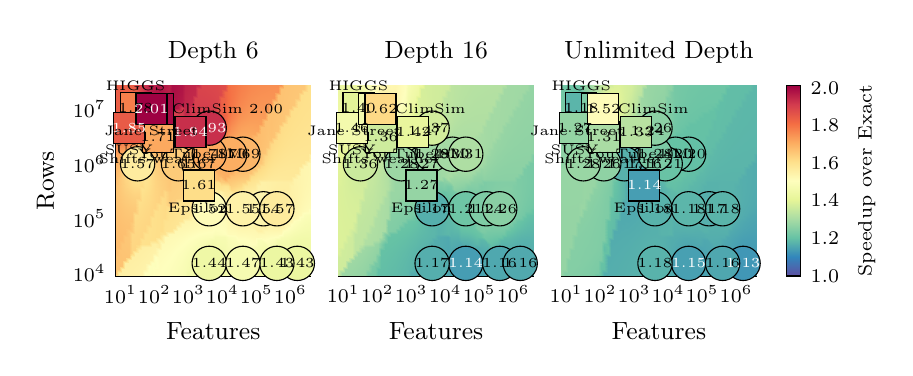
\begin{tikzpicture}
\pgfplotsset{
  colormap={spectralr}{rgb255(0cm)=(94,79,162); rgb255(1cm)=(50,134,188); rgb255(2cm)=(102,194,165); rgb255(3cm)=(169,220,164); rgb255(4cm)=(230,245,152); rgb255(5cm)=(254,254,189); rgb255(6cm)=(254,224,139); rgb255(7cm)=(252,172,96); rgb255(8cm)=(244,109,67); rgb255(9cm)=(211,60,78); rgb255(10cm)=(158,1,66)},
  rcmark/.style={scatter, only marks, scatter src=explicit,
    scatter/use mapped color={draw=black, fill=mapped color, line width=0.4pt}},
  rclabel/.style={only marks, mark=none, point meta=explicit, forget plot,
    nodes near coords={\pgfmathprintnumber[fixed,fixed zerofill,precision=2]{\pgfplotspointmeta}},
    nodes near coords style={font=\fontsize{4.2}{5}\selectfont, anchor=center, inner sep=0pt}},
  rcname/.style={only marks, mark=none, forget plot,
    visualization depends on={value \thisrow{name} \as \nm},
    nodes near coords={\nm}, nodes near coords style={font=\tiny, inner sep=1pt}},
}
\begin{groupplot}[
  group style={group size=3 by 1, horizontal sep=0.35cm, ylabels at=edge left, yticklabels at=edge left},
  width=0.335\linewidth, height=0.33\linewidth, xmode=log, ymode=log,
  point meta min=1.0000, point meta max=2.0129,
  xmin=7.2, xmax=4e+06, ymin=8823.53, ymax=2.73e+07,
  xtick={1e1,1e2,1e3,1e4,1e5,1e6}, ytick={1e4,1e5,1e6,1e7},
  xlabel={Features}, ylabel={Rows}, label style={font=\small}, tick label style={font=\scriptsize},
  title style={font=\small, yshift=-3pt}, tick style={draw=none}, enlargelimits=false, clip=true,
]
\nextgroupplot[title={\strut Depth 6}]
\addplot[surf, shader=interp, point meta=explicit, mesh/rows=60, mesh/cols=60, forget plot] table[x=x, y=y, meta=z] {
x y z
7.2 8823.5 1.6117
9.0095 8823.5 1.5553
11.274 8823.5 1.5542
14.107 8823.5 1.5531
17.652 8823.5 1.5517
22.089 8823.5 1.5501
27.64 8823.5 1.5482
34.587 8823.5 1.5461
43.279 8823.5 1.5437
54.156 8823.5 1.5048
67.767 8823.5 1.5022
84.798 8823.5 1.4995
106.11 8823.5 1.5089
132.78 8823.5 1.5069
166.15 8823.5 1.5047
207.9 8823.5 1.5022
260.15 8823.5 1.4993
325.53 8823.5 1.4961
407.34 8823.5 1.4924
509.72 8823.5 1.4883
637.82 8823.5 1.4838
798.12 8823.5 1.4788
998.7 8823.5 1.4584
1249.7 8823.5 1.4560
1563.8 8823.5 1.4534
1956.8 8823.5 1.4509
2448.5 8823.5 1.4487
3063.9 8823.5 1.4471
3833.9 8823.5 1.4464
4797.5 8823.5 1.4469
6003.2 8823.5 1.4488
7511.9 8823.5 1.4522
9399.8 8823.5 1.4565
11762 8823.5 1.4612
14718 8823.5 1.4683
18417 8823.5 1.4719
23046 8823.5 1.4738
28838 8823.5 1.4696
36085 8823.5 1.4707
45154 8823.5 1.4706
56502 8823.5 1.4691
70702 8823.5 1.4723
88471 8823.5 1.4688
1.1071e+05 8823.5 1.4546
1.3853e+05 8823.5 1.4483
1.7334e+05 8823.5 1.4427
2.1691e+05 8823.5 1.4385
2.7142e+05 8823.5 1.4357
3.3963e+05 8823.5 1.4343
4.2499e+05 8823.5 1.4337
5.318e+05 8823.5 1.4336
6.6545e+05 8823.5 1.4335
8.3269e+05 8823.5 1.4375
1.042e+06 8823.5 1.4364
1.3038e+06 8823.5 1.4352
1.6315e+06 8823.5 1.4346
2.0415e+06 8823.5 1.4351
2.5546e+06 8823.5 1.4364
3.1966e+06 8823.5 1.4383
4e+06 8823.5 1.4404
7.2 10111 1.6679
9.0095 10111 1.5563
11.274 10111 1.5554
14.107 10111 1.5543
17.652 10111 1.5530
22.089 10111 1.5514
27.64 10111 1.5497
34.587 10111 1.5477
43.279 10111 1.5453
54.156 10111 1.5059
67.767 10111 1.5033
84.798 10111 1.5006
106.11 10111 1.5099
132.78 10111 1.5080
166.15 10111 1.5058
207.9 10111 1.5033
260.15 10111 1.5005
325.53 10111 1.4972
407.34 10111 1.4935
509.72 10111 1.4893
637.82 10111 1.4847
798.12 10111 1.4795
998.7 10111 1.4585
1249.7 10111 1.4559
1563.8 10111 1.4531
1956.8 10111 1.4503
2448.5 10111 1.4477
3063.9 10111 1.4458
3833.9 10111 1.4449
4797.5 10111 1.4454
6003.2 10111 1.4475
7511.9 10111 1.4511
9399.8 10111 1.4559
11762 10111 1.4611
14718 10111 1.4686
18417 10111 1.4722
23046 10111 1.4741
28838 10111 1.4709
36085 10111 1.4721
45154 10111 1.4720
56502 10111 1.4705
70702 10111 1.4728
88471 10111 1.4694
1.1071e+05 10111 1.4551
1.3853e+05 10111 1.4482
1.7334e+05 10111 1.4422
2.1691e+05 10111 1.4377
2.7142e+05 10111 1.4349
3.3963e+05 10111 1.4335
4.2499e+05 10111 1.4331
5.318e+05 10111 1.4332
6.6545e+05 10111 1.4369
8.3269e+05 10111 1.4370
1.042e+06 10111 1.4356
1.3038e+06 10111 1.4340
1.6315e+06 10111 1.4333
2.0415e+06 10111 1.4339
2.5546e+06 10111 1.4355
3.1966e+06 10111 1.4376
4e+06 10111 1.4400
7.2 11587 1.6675
9.0095 11587 1.6665
11.274 11587 1.5565
14.107 11587 1.5555
17.652 11587 1.5543
22.089 11587 1.5528
27.64 11587 1.5512
34.587 11587 1.5492
43.279 11587 1.5470
54.156 11587 1.5444
67.767 11587 1.5045
84.798 11587 1.5017
106.11 11587 1.5111
132.78 11587 1.5092
166.15 11587 1.5071
207.9 11587 1.5046
260.15 11587 1.5018
325.53 11587 1.4985
407.34 11587 1.4948
509.72 11587 1.4906
637.82 11587 1.4858
798.12 11587 1.4805
998.7 11587 1.4746
1249.7 11587 1.4560
1563.8 11587 1.4530
1956.8 11587 1.4499
2448.5 11587 1.4470
3063.9 11587 1.4448
3833.9 11587 1.4437
4797.5 11587 1.4441
6003.2 11587 1.4463
7511.9 11587 1.4503
9399.8 11587 1.4555
11762 11587 1.4610
14718 11587 1.4689
18417 11587 1.4726
23046 11587 1.4743
28838 11587 1.4747
36085 11587 1.4732
45154 11587 1.4731
56502 11587 1.4743
70702 11587 1.4733
88471 11587 1.4700
1.1071e+05 11587 1.4652
1.3853e+05 11587 1.4481
1.7334e+05 11587 1.4417
2.1691e+05 11587 1.4371
2.7142e+05 11587 1.4342
3.3963e+05 11587 1.4329
4.2499e+05 11587 1.4326
5.318e+05 11587 1.4348
6.6545e+05 11587 1.4365
8.3269e+05 11587 1.4367
1.042e+06 11587 1.4349
1.3038e+06 11587 1.4329
1.6315e+06 11587 1.4321
2.0415e+06 11587 1.4329
2.5546e+06 11587 1.4347
3.1966e+06 11587 1.4372
4e+06 11587 1.4398
7.2 13278 1.6671
9.0095 13278 1.6660
11.274 13278 1.6650
14.107 13278 1.5567
17.652 13278 1.5556
22.089 13278 1.5543
27.64 13278 1.5527
34.587 13278 1.5509
43.279 13278 1.5487
54.156 13278 1.5462
67.767 13278 1.5058
84.798 13278 1.5030
106.11 13278 1.5000
132.78 13278 1.5105
166.15 13278 1.5084
207.9 13278 1.5060
260.15 13278 1.5033
325.53 13278 1.5001
407.34 13278 1.4964
509.72 13278 1.4922
637.82 13278 1.4874
798.12 13278 1.4819
998.7 13278 1.4758
1249.7 13278 1.4692
1563.8 13278 1.4532
1956.8 13278 1.4499
2448.5 13278 1.4467
3063.9 13278 1.4441
3833.9 13278 1.4428
4797.5 13278 1.4432
6003.2 13278 1.4457
7511.9 13278 1.4499
9399.8 13278 1.4554
11762 13278 1.4612
14718 13278 1.4694
18417 13278 1.4731
23046 13278 1.4746
28838 13278 1.4747
36085 13278 1.4738
45154 13278 1.4738
56502 13278 1.4744
70702 13278 1.4736
88471 13278 1.4706
1.1071e+05 13278 1.4659
1.3853e+05 13278 1.4589
1.7334e+05 13278 1.4414
2.1691e+05 13278 1.4367
2.7142e+05 13278 1.4338
3.3963e+05 13278 1.4325
4.2499e+05 13278 1.4323
5.318e+05 13278 1.4341
6.6545e+05 13278 1.4363
8.3269e+05 13278 1.4367
1.042e+06 13278 1.4345
1.3038e+06 13278 1.4321
1.6315e+06 13278 1.4313
2.0415e+06 13278 1.4323
2.5546e+06 13278 1.4343
3.1966e+06 13278 1.4370
4e+06 13278 1.4399
7.2 15216 1.6666
9.0095 15216 1.6655
11.274 15216 1.6644
14.107 15216 1.5580
17.652 15216 1.5569
22.089 15216 1.5557
27.64 15216 1.5543
34.587 15216 1.5525
43.279 15216 1.5505
54.156 15216 1.5481
67.767 15216 1.5453
84.798 15216 1.5043
106.11 15216 1.5013
132.78 15216 1.5119
166.15 15216 1.5099
207.9 15216 1.5076
260.15 15216 1.5049
325.53 15216 1.5018
407.34 15216 1.4982
509.72 15216 1.4941
637.82 15216 1.4892
798.12 15216 1.4837
998.7 15216 1.4775
1249.7 15216 1.4707
1563.8 15216 1.4538
1956.8 15216 1.4502
2448.5 15216 1.4468
3063.9 15216 1.4440
3833.9 15216 1.4426
4797.5 15216 1.4430
6003.2 15216 1.4456
7511.9 15216 1.4501
9399.8 15216 1.4557
11762 15216 1.4616
14718 15216 1.4700
18417 15216 1.4736
23046 15216 1.4749
28838 15216 1.4748
36085 15216 1.4743
45154 15216 1.4743
56502 15216 1.4745
70702 15216 1.4740
88471 15216 1.4711
1.1071e+05 15216 1.4666
1.3853e+05 15216 1.4598
1.7334e+05 15216 1.4414
2.1691e+05 15216 1.4366
2.7142e+05 15216 1.4337
3.3963e+05 15216 1.4324
4.2499e+05 15216 1.4322
5.318e+05 15216 1.4340
6.6545e+05 15216 1.4366
8.3269e+05 15216 1.4371
1.042e+06 15216 1.4346
1.3038e+06 15216 1.4319
1.6315e+06 15216 1.4311
2.0415e+06 15216 1.4321
2.5546e+06 15216 1.4344
3.1966e+06 15216 1.4372
4e+06 15216 1.4402
7.2 17436 1.6662
9.0095 17436 1.6650
11.274 17436 1.6639
14.107 17436 1.6628
17.652 17436 1.5583
22.089 17436 1.5572
27.64 17436 1.5559
34.587 17436 1.5543
43.279 17436 1.5524
54.156 17436 1.5501
67.767 17436 1.5475
84.798 17436 1.5443
106.11 17436 1.5027
132.78 17436 1.5134
166.15 17436 1.5115
207.9 17436 1.5093
260.15 17436 1.5068
325.53 17436 1.5038
407.34 17436 1.5003
509.72 17436 1.4962
637.82 17436 1.4915
798.12 17436 1.4861
998.7 17436 1.4799
1249.7 17436 1.4729
1563.8 17436 1.4655
1956.8 17436 1.4512
2448.5 17436 1.4475
3063.9 17436 1.4446
3833.9 17436 1.4431
4797.5 17436 1.4435
6003.2 17436 1.4463
7511.9 17436 1.4509
9399.8 17436 1.4565
11762 17436 1.4623
14718 17436 1.4709
18417 17436 1.4744
23046 17436 1.4755
28838 17436 1.4751
36085 17436 1.4745
45154 17436 1.4745
56502 17436 1.4748
70702 17436 1.4745
88471 17436 1.4718
1.1071e+05 17436 1.4677
1.3853e+05 17436 1.4611
1.7334e+05 17436 1.4528
2.1691e+05 17436 1.4367
2.7142e+05 17436 1.4339
3.3963e+05 17436 1.4326
4.2499e+05 17436 1.4329
5.318e+05 17436 1.4348
6.6545e+05 17436 1.4376
8.3269e+05 17436 1.4380
1.042e+06 17436 1.4354
1.3038e+06 17436 1.4325
1.6315e+06 17436 1.4315
2.0415e+06 17436 1.4326
2.5546e+06 17436 1.4349
3.1966e+06 17436 1.4379
4e+06 17436 1.4410
7.2 19981 1.6657
9.0095 19981 1.6644
11.274 19981 1.6633
14.107 19981 1.6622
17.652 19981 1.6612
22.089 19981 1.5587
27.64 19981 1.5575
34.587 19981 1.5560
43.279 19981 1.5543
54.156 19981 1.5522
67.767 19981 1.5497
84.798 19981 1.5467
106.11 19981 1.5041
132.78 19981 1.5150
166.15 19981 1.5133
207.9 19981 1.5112
260.15 19981 1.5088
325.53 19981 1.5060
407.34 19981 1.5026
509.72 19981 1.4987
637.82 19981 1.4942
798.12 19981 1.4889
998.7 19981 1.4828
1249.7 19981 1.4759
1563.8 19981 1.4685
1956.8 19981 1.4608
2448.5 19981 1.4491
3063.9 19981 1.4460
3833.9 19981 1.4445
4797.5 19981 1.4450
6003.2 19981 1.4479
7511.9 19981 1.4525
9399.8 19981 1.4579
11762 19981 1.4632
14718 19981 1.4720
18417 19981 1.4754
23046 19981 1.4763
28838 19981 1.4759
36085 19981 1.4752
45154 19981 1.4751
56502 19981 1.4755
70702 19981 1.4753
88471 19981 1.4728
1.1071e+05 19981 1.4691
1.3853e+05 19981 1.4631
1.7334e+05 19981 1.4551
2.1691e+05 19981 1.4372
2.7142e+05 19981 1.4344
3.3963e+05 19981 1.4356
4.2499e+05 19981 1.4348
5.318e+05 19981 1.4367
6.6545e+05 19981 1.4393
8.3269e+05 19981 1.4396
1.042e+06 19981 1.4370
1.3038e+06 19981 1.4340
1.6315e+06 19981 1.4329
2.0415e+06 19981 1.4339
2.5546e+06 19981 1.4361
3.1966e+06 19981 1.4390
4e+06 19981 1.4421
7.2 22897 1.6809
9.0095 22897 1.6639
11.274 22897 1.6626
14.107 22897 1.6614
17.652 22897 1.6604
22.089 22897 1.6275
27.64 22897 1.5591
34.587 22897 1.5578
43.279 22897 1.5562
54.156 22897 1.5543
67.767 22897 1.5520
84.798 22897 1.5492
106.11 22897 1.5459
132.78 22897 1.5167
166.15 22897 1.5151
207.9 22897 1.5132
260.15 22897 1.5110
325.53 22897 1.5083
407.34 22897 1.5052
509.72 22897 1.5015
637.82 22897 1.4972
798.12 22897 1.4922
998.7 22897 1.4863
1249.7 22897 1.4797
1563.8 22897 1.4724
1956.8 22897 1.4649
2448.5 22897 1.4514
3063.9 22897 1.4485
3833.9 22897 1.4470
4797.5 22897 1.4476
6003.2 22897 1.4504
7511.9 22897 1.4548
9399.8 22897 1.4598
11762 22897 1.4646
14718 22897 1.4736
18417 22897 1.4768
23046 22897 1.4777
28838 22897 1.4773
36085 22897 1.4767
45154 22897 1.4764
56502 22897 1.4768
70702 22897 1.4766
88471 22897 1.4741
1.1071e+05 22897 1.4711
1.3853e+05 22897 1.4657
1.7334e+05 22897 1.4583
2.1691e+05 22897 1.4502
2.7142e+05 22897 1.4425
3.3963e+05 22897 1.4391
4.2499e+05 22897 1.4383
5.318e+05 22897 1.4399
6.6545e+05 22897 1.4420
8.3269e+05 22897 1.4420
1.042e+06 22897 1.4394
1.3038e+06 22897 1.4365
1.6315e+06 22897 1.4352
2.0415e+06 22897 1.4360
2.5546e+06 22897 1.4380
3.1966e+06 22897 1.4408
4e+06 22897 1.4437
7.2 26238 1.6802
9.0095 26238 1.6633
11.274 26238 1.6619
14.107 26238 1.6607
17.652 26238 1.6596
22.089 26238 1.6268
27.64 26238 1.6276
34.587 26238 1.5595
43.279 26238 1.5581
54.156 26238 1.5564
67.767 26238 1.5543
84.798 26238 1.5518
106.11 26238 1.5487
132.78 26238 1.5185
166.15 26238 1.5171
207.9 26238 1.5154
260.15 26238 1.5133
325.53 26238 1.5109
407.34 26238 1.5080
509.72 26238 1.5046
637.82 26238 1.5006
798.12 26238 1.4959
998.7 26238 1.4904
1249.7 26238 1.4842
1563.8 26238 1.4774
1956.8 26238 1.4702
2448.5 26238 1.4634
3063.9 26238 1.4520
3833.9 26238 1.4507
4797.5 26238 1.4513
6003.2 26238 1.4540
7511.9 26238 1.4579
9399.8 26238 1.4623
11762 26238 1.4663
14718 26238 1.4756
18417 26238 1.4788
23046 26238 1.4799
28838 26238 1.4796
36085 26238 1.4792
45154 26238 1.4849
56502 26238 1.4880
70702 26238 1.4786
88471 26238 1.4760
1.1071e+05 26238 1.4737
1.3853e+05 26238 1.4692
1.7334e+05 26238 1.4626
2.1691e+05 26238 1.4549
2.7142e+05 26238 1.4596
3.3963e+05 26238 1.4445
4.2499e+05 26238 1.4435
5.318e+05 26238 1.4447
6.6545e+05 26238 1.4460
8.3269e+05 26238 1.4455
1.042e+06 26238 1.4429
1.3038e+06 26238 1.4400
1.6315e+06 26238 1.4385
2.0415e+06 26238 1.4389
2.5546e+06 26238 1.4406
3.1966e+06 26238 1.4430
4e+06 26238 1.4457
7.2 30067 1.6794
9.0095 30067 1.6780
11.274 30067 1.6612
14.107 30067 1.6599
17.652 30067 1.6587
22.089 30067 1.6261
27.64 30067 1.6269
34.587 30067 1.6030
43.279 30067 1.5601
54.156 30067 1.5586
67.767 30067 1.5567
84.798 30067 1.5544
106.11 30067 1.5516
132.78 30067 1.5623
166.15 30067 1.5191
207.9 30067 1.5176
260.15 30067 1.5158
325.53 30067 1.5136
407.34 30067 1.5111
509.72 30067 1.5080
637.82 30067 1.5043
798.12 30067 1.5000
998.7 30067 1.4951
1249.7 30067 1.4894
1563.8 30067 1.4832
1956.8 30067 1.4767
2448.5 30067 1.4706
3063.9 30067 1.4656
3833.9 30067 1.4556
4797.5 30067 1.4562
6003.2 30067 1.4585
7511.9 30067 1.4617
9399.8 30067 1.4652
11762 30067 1.4684
14718 30067 1.4783
18417 30067 1.4816
23046 30067 1.4830
28838 30067 1.4830
36085 30067 1.4904
45154 30067 1.4911
56502 30067 1.4940
70702 30067 1.4985
88471 30067 1.4787
1.1071e+05 30067 1.4772
1.3853e+05 30067 1.4736
1.7334e+05 30067 1.4679
2.1691e+05 30067 1.4787
2.7142e+05 30067 1.4708
3.3963e+05 30067 1.4519
4.2499e+05 30067 1.4507
5.318e+05 30067 1.4510
6.6545e+05 30067 1.4515
8.3269e+05 30067 1.4503
1.042e+06 30067 1.4474
1.3038e+06 30067 1.4444
1.6315e+06 30067 1.4427
2.0415e+06 30067 1.4426
2.5546e+06 30067 1.4439
3.1966e+06 30067 1.4458
4e+06 30067 1.4481
7.2 34455 1.6786
9.0095 34455 1.6771
11.274 34455 1.6604
14.107 34455 1.6590
17.652 34455 1.6578
22.089 34455 1.6253
27.64 34455 1.6261
34.587 34455 1.6271
43.279 34455 1.6036
54.156 34455 1.6049
67.767 34455 1.6063
84.798 34455 1.5571
106.11 34455 1.5545
132.78 34455 1.5657
166.15 34455 1.5212
207.9 34455 1.5199
260.15 34455 1.5184
325.53 34455 1.5165
407.34 34455 1.5143
509.72 34455 1.5116
637.82 34455 1.5083
798.12 34455 1.5045
998.7 34455 1.5001
1249.7 34455 1.4951
1563.8 34455 1.4897
1956.8 34455 1.4841
2448.5 34455 1.4788
3063.9 34455 1.4745
3833.9 34455 1.4617
4797.5 34455 1.4622
6003.2 34455 1.4639
7511.9 34455 1.4663
9399.8 34455 1.4687
11762 34455 1.4708
14718 34455 1.4816
18417 34455 1.4852
23046 34455 1.4870
28838 34455 1.4877
36085 34455 1.4975
45154 34455 1.4983
56502 34455 1.5009
70702 34455 1.5048
88471 34455 1.5091
1.1071e+05 34455 1.4816
1.3853e+05 34455 1.4789
1.7334e+05 34455 1.4742
2.1691e+05 34455 1.4900
2.7142e+05 34455 1.4836
3.3963e+05 34455 1.4787
4.2499e+05 34455 1.4598
5.318e+05 34455 1.4593
6.6545e+05 34455 1.4586
8.3269e+05 34455 1.4565
1.042e+06 34455 1.4532
1.3038e+06 34455 1.4499
1.6315e+06 34455 1.4477
2.0415e+06 34455 1.4471
2.5546e+06 34455 1.4478
3.1966e+06 34455 1.4492
4e+06 34455 1.4510
7.2 39484 1.6777
9.0095 39484 1.6761
11.274 39484 1.6747
14.107 39484 1.6581
17.652 39484 1.6568
22.089 39484 1.6244
27.64 39484 1.6253
34.587 39484 1.6264
43.279 39484 1.6031
54.156 39484 1.6045
67.767 39484 1.6060
84.798 39484 1.6075
106.11 39484 1.6090
132.78 39484 1.5548
166.15 39484 1.5667
207.9 39484 1.5224
260.15 39484 1.5211
325.53 39484 1.5195
407.34 39484 1.5176
509.72 39484 1.5153
637.82 39484 1.5125
798.12 39484 1.5092
998.7 39484 1.5054
1249.7 39484 1.5012
1563.8 39484 1.4966
1956.8 39484 1.4920
2448.5 39484 1.4877
3063.9 39484 1.4842
3833.9 39484 1.4822
4797.5 39484 1.4691
6003.2 39484 1.4700
7511.9 39484 1.4714
9399.8 39484 1.4727
11762 39484 1.4737
14718 39484 1.4856
18417 39484 1.4896
23046 39484 1.4922
28838 39484 1.5056
36085 39484 1.5053
45154 39484 1.5062
56502 39484 1.5083
70702 39484 1.5113
88471 39484 1.5148
1.1071e+05 39484 1.4869
1.3853e+05 39484 1.4853
1.7334e+05 39484 1.5062
2.1691e+05 39484 1.5016
2.7142e+05 39484 1.4969
3.3963e+05 39484 1.4932
4.2499e+05 39484 1.4711
5.318e+05 39484 1.4696
6.6545e+05 39484 1.4676
8.3269e+05 39484 1.4644
1.042e+06 39484 1.4603
1.3038e+06 39484 1.4564
1.6315e+06 39484 1.4536
2.0415e+06 39484 1.4523
2.5546e+06 39484 1.4522
3.1966e+06 39484 1.4530
4e+06 39484 1.4542
7.2 45246 1.6769
9.0095 45246 1.6751
11.274 45246 1.6735
14.107 45246 1.6571
17.652 45246 1.6557
22.089 45246 1.6235
27.64 45246 1.6244
34.587 45246 1.6255
43.279 45246 1.6268
54.156 45246 1.6040
67.767 45246 1.6056
84.798 45246 1.6072
106.11 45246 1.6089
132.78 45246 1.6105
166.15 45246 1.5706
207.9 45246 1.5249
260.15 45246 1.5239
325.53 45246 1.5227
407.34 45246 1.5211
509.72 45246 1.5192
637.82 45246 1.5169
798.12 45246 1.5141
998.7 45246 1.5109
1249.7 45246 1.5074
1563.8 45246 1.5036
1956.8 45246 1.4999
2448.5 45246 1.4966
3063.9 45246 1.4939
3833.9 45246 1.4923
4797.5 45246 1.4917
6003.2 45246 1.4768
7511.9 45246 1.4769
9399.8 45246 1.4770
11762 45246 1.4770
14718 45246 1.4903
18417 45246 1.4949
23046 45246 1.4982
28838 45246 1.5130
36085 45246 1.5133
45154 45246 1.5141
56502 45246 1.5156
70702 45246 1.5177
88471 45246 1.5202
1.1071e+05 45246 1.5227
1.3853e+05 45246 1.5176
1.7334e+05 45246 1.5153
2.1691e+05 45246 1.5126
2.7142e+05 45246 1.5097
3.3963e+05 45246 1.5073
4.2499e+05 45246 1.5057
5.318e+05 45246 1.4819
6.6545e+05 45246 1.4783
8.3269e+05 45246 1.4737
1.042e+06 45246 1.4686
1.3038e+06 45246 1.4638
1.6315e+06 45246 1.4602
2.0415e+06 45246 1.4580
2.5546e+06 45246 1.4571
3.1966e+06 45246 1.4572
4e+06 45246 1.4578
7.2 51849 1.6759
9.0095 51849 1.6740
11.274 51849 1.6723
14.107 51849 1.6707
17.652 51849 1.6545
22.089 51849 1.6225
27.64 51849 1.6234
34.587 51849 1.6246
43.279 51849 1.6260
54.156 51849 1.6035
67.767 51849 1.6052
84.798 51849 1.6070
106.11 51849 1.6088
132.78 51849 1.6105
166.15 51849 1.5963
207.9 51849 1.5946
260.15 51849 1.5268
325.53 51849 1.5259
407.34 51849 1.5247
509.72 51849 1.5232
637.82 51849 1.5214
798.12 51849 1.5191
998.7 51849 1.5164
1249.7 51849 1.5135
1563.8 51849 1.5104
1956.8 51849 1.5074
2448.5 51849 1.5048
3063.9 51849 1.5028
3833.9 51849 1.5015
4797.5 51849 1.5006
6003.2 51849 1.4936
7511.9 51849 1.4958
9399.8 51849 1.4991
11762 51849 1.5038
14718 51849 1.5155
18417 51849 1.5159
23046 51849 1.5163
28838 51849 1.5202
36085 51849 1.5209
45154 51849 1.5216
56502 51849 1.5224
70702 51849 1.5235
88471 51849 1.5251
1.1071e+05 51849 1.5268
1.3853e+05 51849 1.5243
1.7334e+05 51849 1.5235
2.1691e+05 51849 1.5224
2.7142e+05 51849 1.5212
3.3963e+05 51849 1.5202
4.2499e+05 51849 1.5191
5.318e+05 51849 1.5179
6.6545e+05 51849 1.4907
8.3269e+05 51849 1.4844
1.042e+06 51849 1.4779
1.3038e+06 51849 1.4720
1.6315e+06 51849 1.4673
2.0415e+06 51849 1.4642
2.5546e+06 51849 1.4624
3.1966e+06 51849 1.4616
4e+06 51849 1.4616
7.2 59416 1.6750
9.0095 59416 1.6729
11.274 59416 1.6710
14.107 59416 1.6693
17.652 59416 1.6533
22.089 59416 1.6519
27.64 59416 1.6224
34.587 59416 1.6236
43.279 59416 1.6251
54.156 59416 1.6268
67.767 59416 1.6047
84.798 59416 1.6067
106.11 59416 1.6086
132.78 59416 1.6105
166.15 59416 1.6123
207.9 59416 1.5959
260.15 59416 1.5939
325.53 59416 1.5915
407.34 59416 1.5283
509.72 59416 1.5273
637.82 59416 1.5259
798.12 59416 1.5241
998.7 59416 1.5219
1249.7 59416 1.5194
1563.8 59416 1.5167
1956.8 59416 1.5142
2448.5 59416 1.5120
3063.9 59416 1.5103
3833.9 59416 1.5091
4797.5 59416 1.5081
6003.2 59416 1.5000
7511.9 59416 1.5014
9399.8 59416 1.5040
11762 59416 1.5082
14718 59416 1.5189
18417 59416 1.5204
23046 59416 1.5221
28838 59416 1.5268
36085 59416 1.5278
45154 59416 1.5282
56502 59416 1.5283
70702 59416 1.5286
88471 59416 1.5293
1.1071e+05 59416 1.5489
1.3853e+05 59416 1.5495
1.7334e+05 59416 1.5302
2.1691e+05 59416 1.5305
2.7142e+05 59416 1.5309
3.3963e+05 59416 1.5313
4.2499e+05 59416 1.5310
5.318e+05 59416 1.5296
6.6545e+05 59416 1.5039
8.3269e+05 59416 1.4960
1.042e+06 59416 1.4879
1.3038e+06 59416 1.4807
1.6315e+06 59416 1.4749
2.0415e+06 59416 1.4707
2.5546e+06 59416 1.4679
3.1966e+06 59416 1.4663
4e+06 59416 1.4655
7.2 68087 1.6740
9.0095 68087 1.6717
11.274 68087 1.6696
14.107 68087 1.6677
17.652 68087 1.6662
22.089 68087 1.6505
27.64 68087 1.6212
34.587 68087 1.6225
43.279 68087 1.6241
54.156 68087 1.6260
67.767 68087 1.6042
84.798 68087 1.6063
106.11 68087 1.6084
132.78 68087 1.6105
166.15 68087 1.6124
207.9 68087 1.5973
260.15 68087 1.5953
325.53 68087 1.5929
407.34 68087 1.5901
509.72 68087 1.5314
637.82 68087 1.5304
798.12 68087 1.5291
998.7 68087 1.5273
1249.7 68087 1.5250
1563.8 68087 1.5225
1956.8 68087 1.5200
2448.5 68087 1.5177
3063.9 68087 1.5160
3833.9 68087 1.5148
4797.5 68087 1.5138
6003.2 68087 1.5054
7511.9 68087 1.5060
9399.8 68087 1.5081
11762 68087 1.5120
14718 68087 1.5219
18417 68087 1.5244
23046 68087 1.5272
28838 68087 1.5325
36085 68087 1.5337
45154 68087 1.5339
56502 68087 1.5333
70702 68087 1.5327
88471 68087 1.5482
1.1071e+05 68087 1.5481
1.3853e+05 68087 1.5485
1.7334e+05 68087 1.5500
2.1691e+05 68087 1.5368
2.7142e+05 68087 1.5388
3.3963e+05 68087 1.5407
4.2499e+05 68087 1.5413
5.318e+05 68087 1.5397
6.6545e+05 68087 1.5366
8.3269e+05 68087 1.5078
1.042e+06 68087 1.4981
1.3038e+06 68087 1.4895
1.6315e+06 68087 1.4825
2.0415e+06 68087 1.4772
2.5546e+06 68087 1.4735
3.1966e+06 68087 1.4711
4e+06 68087 1.4695
7.2 78023 1.6730
9.0095 78023 1.6705
11.274 78023 1.6681
14.107 78023 1.6660
17.652 78023 1.6643
22.089 78023 1.6489
27.64 78023 1.6199
34.587 78023 1.6213
43.279 78023 1.6231
54.156 78023 1.6251
67.767 78023 1.6273
84.798 78023 1.6059
106.11 78023 1.6082
132.78 78023 1.6105
166.15 78023 1.6126
207.9 78023 1.5988
260.15 78023 1.5969
325.53 78023 1.5945
407.34 78023 1.5917
509.72 78023 1.5882
637.82 78023 1.5350
798.12 78023 1.5341
998.7 78023 1.5326
1249.7 78023 1.5304
1563.8 78023 1.5278
1956.8 78023 1.5248
2448.5 78023 1.5220
3063.9 78023 1.5199
3833.9 78023 1.5185
4797.5 78023 1.5175
6003.2 78023 1.5167
7511.9 78023 1.5097
9399.8 78023 1.5114
11762 78023 1.5151
14718 78023 1.5245
18417 78023 1.5280
23046 78023 1.5318
28838 78023 1.5373
36085 78023 1.5386
45154 78023 1.5386
56502 78023 1.5375
70702 78023 1.5361
88471 78023 1.5476
1.1071e+05 78023 1.5471
1.3853e+05 78023 1.5473
1.7334e+05 78023 1.5487
2.1691e+05 78023 1.5413
2.7142e+05 78023 1.5449
3.3963e+05 78023 1.5485
4.2499e+05 78023 1.5499
5.318e+05 78023 1.5483
6.6545e+05 78023 1.5445
8.3269e+05 78023 1.5389
1.042e+06 78023 1.5080
1.3038e+06 78023 1.4981
1.6315e+06 78023 1.4900
2.0415e+06 78023 1.4837
2.5546e+06 78023 1.4791
3.1966e+06 78023 1.4758
4e+06 78023 1.4736
7.2 89410 1.6720
9.0095 89410 1.6692
11.274 89410 1.6666
14.107 89410 1.6643
17.652 89410 1.6624
22.089 89410 1.6609
27.64 89410 1.6185
34.587 89410 1.6200
43.279 89410 1.6219
54.156 89410 1.6241
67.767 89410 1.6265
84.798 89410 1.6055
106.11 89410 1.6080
132.78 89410 1.6105
166.15 89410 1.6128
207.9 89410 1.6005
260.15 89410 1.5987
325.53 89410 1.5963
407.34 89410 1.5935
509.72 89410 1.5900
637.82 89410 1.5859
798.12 89410 1.5390
998.7 89410 1.5378
1249.7 89410 1.5357
1563.8 89410 1.5326
1956.8 89410 1.5289
2448.5 89410 1.5250
3063.9 89410 1.5220
3833.9 89410 1.5202
4797.5 89410 1.5194
6003.2 89410 1.5191
7511.9 89410 1.5124
9399.8 89410 1.5139
11762 89410 1.5176
14718 89410 1.5267
18417 89410 1.5310
23046 89410 1.5355
28838 89410 1.5410
36085 89410 1.5425
45154 89410 1.5424
56502 89410 1.5407
70702 89410 1.5479
88471 89410 1.5470
1.1071e+05 89410 1.5461
1.3853e+05 89410 1.5457
1.7334e+05 89410 1.5471
2.1691e+05 89410 1.5511
2.7142e+05 89410 1.5496
3.3963e+05 89410 1.5551
4.2499e+05 89410 1.5572
5.318e+05 89410 1.5554
6.6545e+05 89410 1.5510
8.3269e+05 89410 1.5449
1.042e+06 89410 1.5360
1.3038e+06 89410 1.5061
1.6315e+06 89410 1.4970
2.0415e+06 89410 1.4898
2.5546e+06 89410 1.4844
3.1966e+06 89410 1.4804
4e+06 89410 1.4776
7.2 1.0246e+05 1.6709
9.0095 1.0246e+05 1.6678
11.274 1.0246e+05 1.6649
14.107 1.0246e+05 1.6623
17.652 1.0246e+05 1.6602
22.089 1.0246e+05 1.6586
27.64 1.0246e+05 1.6170
34.587 1.0246e+05 1.6186
43.279 1.0246e+05 1.6206
54.156 1.0246e+05 1.6229
67.767 1.0246e+05 1.6256
84.798 1.0246e+05 1.6050
106.11 1.0246e+05 1.6078
132.78 1.0246e+05 1.6105
166.15 1.0246e+05 1.6130
207.9 1.0246e+05 1.6153
260.15 1.0246e+05 1.6006
325.53 1.0246e+05 1.5983
407.34 1.0246e+05 1.5955
509.72 1.0246e+05 1.5921
637.82 1.0246e+05 1.5880
798.12 1.0246e+05 1.5831
998.7 1.0246e+05 1.5773
1249.7 1.0246e+05 1.5410
1563.8 1.0246e+05 1.5374
1956.8 1.0246e+05 1.5325
2448.5 1.0246e+05 1.5271
3063.9 1.0246e+05 1.5226
3833.9 1.0246e+05 1.5203
4797.5 1.0246e+05 1.5199
6003.2 1.0246e+05 1.5272
7511.9 1.0246e+05 1.5318
9399.8 1.0246e+05 1.5368
11762 1.0246e+05 1.5196
14718 1.0246e+05 1.5284
18417 1.0246e+05 1.5335
23046 1.0246e+05 1.5444
28838 1.0246e+05 1.5438
36085 1.0246e+05 1.5454
45154 1.0246e+05 1.5452
56502 1.0246e+05 1.5432
70702 1.0246e+05 1.5478
88471 1.0246e+05 1.5465
1.1071e+05 1.0246e+05 1.5450
1.3853e+05 1.0246e+05 1.5440
1.7334e+05 1.0246e+05 1.5449
2.1691e+05 1.0246e+05 1.5498
2.7142e+05 1.0246e+05 1.5582
3.3963e+05 1.0246e+05 1.5607
4.2499e+05 1.0246e+05 1.5632
5.318e+05 1.0246e+05 1.5610
6.6545e+05 1.0246e+05 1.5560
8.3269e+05 1.0246e+05 1.5497
1.042e+06 1.0246e+05 1.5412
1.3038e+06 1.0246e+05 1.5324
1.6315e+06 1.0246e+05 1.5242
2.0415e+06 1.0246e+05 1.4955
2.5546e+06 1.0246e+05 1.4894
3.1966e+06 1.0246e+05 1.4848
4e+06 1.0246e+05 1.4814
7.2 1.1741e+05 1.6699
9.0095 1.1741e+05 1.6665
11.274 1.1741e+05 1.6632
14.107 1.1741e+05 1.6603
17.652 1.1741e+05 1.6579
22.089 1.1741e+05 1.6561
27.64 1.1741e+05 1.6153
34.587 1.1741e+05 1.6170
43.279 1.1741e+05 1.6191
54.156 1.1741e+05 1.6217
67.767 1.1741e+05 1.6247
84.798 1.1741e+05 1.6278
106.11 1.1741e+05 1.6075
132.78 1.1741e+05 1.6105
166.15 1.1741e+05 1.6133
207.9 1.1741e+05 1.6157
260.15 1.1741e+05 1.6026
325.53 1.1741e+05 1.6005
407.34 1.1741e+05 1.5978
509.72 1.1741e+05 1.5944
637.82 1.1741e+05 1.5904
798.12 1.1741e+05 1.5856
998.7 1.1741e+05 1.5798
1249.7 1.1741e+05 1.5763
1563.8 1.1741e+05 1.5673
1956.8 1.1741e+05 1.5553
2448.5 1.1741e+05 1.5288
3063.9 1.1741e+05 1.5224
3833.9 1.1741e+05 1.5193
4797.5 1.1741e+05 1.5193
6003.2 1.1741e+05 1.5253
7511.9 1.1741e+05 1.5308
9399.8 1.1741e+05 1.5364
11762 1.1741e+05 1.5412
14718 1.1741e+05 1.5298
18417 1.1741e+05 1.5416
23046 1.1741e+05 1.5450
28838 1.1741e+05 1.5471
36085 1.1741e+05 1.5473
45154 1.1741e+05 1.5472
56502 1.1741e+05 1.5485
70702 1.1741e+05 1.5477
88471 1.1741e+05 1.5460
1.1071e+05 1.1741e+05 1.5439
1.3853e+05 1.1741e+05 1.5422
1.7334e+05 1.1741e+05 1.5426
2.1691e+05 1.1741e+05 1.5482
2.7142e+05 1.1741e+05 1.5592
3.3963e+05 1.1741e+05 1.5654
4.2499e+05 1.1741e+05 1.5679
5.318e+05 1.1741e+05 1.5650
6.6545e+05 1.1741e+05 1.5596
8.3269e+05 1.1741e+05 1.5532
1.042e+06 1.1741e+05 1.5451
1.3038e+06 1.1741e+05 1.5367
1.6315e+06 1.1741e+05 1.5288
2.0415e+06 1.1741e+05 1.5218
2.5546e+06 1.1741e+05 1.4940
3.1966e+06 1.1741e+05 1.4889
4e+06 1.1741e+05 1.4850
7.2 1.3455e+05 1.6689
9.0095 1.3455e+05 1.6650
11.274 1.3455e+05 1.6614
14.107 1.3455e+05 1.6581
17.652 1.3455e+05 1.6553
22.089 1.3455e+05 1.6533
27.64 1.3455e+05 1.6521
34.587 1.3455e+05 1.6152
43.279 1.3455e+05 1.6175
54.156 1.3455e+05 1.6203
67.767 1.3455e+05 1.6236
84.798 1.3455e+05 1.6271
106.11 1.3455e+05 1.6072
132.78 1.3455e+05 1.6105
166.15 1.3455e+05 1.6136
207.9 1.3455e+05 1.6163
260.15 1.3455e+05 1.6049
325.53 1.3455e+05 1.6029
407.34 1.3455e+05 1.6002
509.72 1.3455e+05 1.5970
637.82 1.3455e+05 1.5931
798.12 1.3455e+05 1.5885
998.7 1.3455e+05 1.5830
1249.7 1.3455e+05 1.5799
1563.8 1.3455e+05 1.5710
1956.8 1.3455e+05 1.5582
2448.5 1.3455e+05 1.5419
3063.9 1.3455e+05 1.5267
3833.9 1.3455e+05 1.5189
4797.5 1.3455e+05 1.5194
6003.2 1.3455e+05 1.5243
7511.9 1.3455e+05 1.5305
9399.8 1.3455e+05 1.5364
11762 1.3455e+05 1.5414
14718 1.3455e+05 1.5450
18417 1.3455e+05 1.5419
23046 1.3455e+05 1.5454
28838 1.3455e+05 1.5475
36085 1.3455e+05 1.5485
45154 1.3455e+05 1.5487
56502 1.3455e+05 1.5485
70702 1.3455e+05 1.5476
88471 1.3455e+05 1.5457
1.1071e+05 1.3455e+05 1.5432
1.3853e+05 1.3455e+05 1.5409
1.7334e+05 1.3455e+05 1.5407
2.1691e+05 1.3455e+05 1.5467
2.7142e+05 1.3455e+05 1.5600
3.3963e+05 1.3455e+05 1.5695
4.2499e+05 1.3455e+05 1.5707
5.318e+05 1.3455e+05 1.5674
6.6545e+05 1.3455e+05 1.5618
8.3269e+05 1.3455e+05 1.5555
1.042e+06 1.3455e+05 1.5479
1.3038e+06 1.3455e+05 1.5400
1.6315e+06 1.3455e+05 1.5325
2.0415e+06 1.3455e+05 1.5257
2.5546e+06 1.3455e+05 1.5198
3.1966e+06 1.3455e+05 1.5150
4e+06 1.3455e+05 1.4883
7.2 1.5418e+05 1.6678
9.0095 1.5418e+05 1.6636
11.274 1.5418e+05 1.6595
14.107 1.5418e+05 1.6557
17.652 1.5418e+05 1.6526
22.089 1.5418e+05 1.6503
27.64 1.5418e+05 1.6489
34.587 1.5418e+05 1.6132
43.279 1.5418e+05 1.6157
54.156 1.5418e+05 1.6188
67.767 1.5418e+05 1.6224
84.798 1.5418e+05 1.6263
106.11 1.5418e+05 1.6302
132.78 1.5418e+05 1.6106
166.15 1.5418e+05 1.6140
207.9 1.5418e+05 1.6169
260.15 1.5418e+05 1.6073
325.53 1.5418e+05 1.6054
407.34 1.5418e+05 1.6029
509.72 1.5418e+05 1.5998
637.82 1.5418e+05 1.5960
798.12 1.5418e+05 1.5916
998.7 1.5418e+05 1.5866
1249.7 1.5418e+05 1.5843
1563.8 1.5418e+05 1.5762
1956.8 1.5418e+05 1.5634
2448.5 1.5418e+05 1.5454
3063.9 1.5418e+05 1.5273
3833.9 1.5418e+05 1.5179
4797.5 1.5418e+05 1.5197
6003.2 1.5418e+05 1.5245
7511.9 1.5418e+05 1.5310
9399.8 1.5418e+05 1.5370
11762 1.5418e+05 1.5419
14718 1.5418e+05 1.5454
18417 1.5418e+05 1.5419
23046 1.5418e+05 1.5454
28838 1.5418e+05 1.5476
36085 1.5418e+05 1.5486
45154 1.5418e+05 1.5488
56502 1.5418e+05 1.5485
70702 1.5418e+05 1.5476
88471 1.5418e+05 1.5456
1.1071e+05 1.5418e+05 1.5430
1.3853e+05 1.5418e+05 1.5406
1.7334e+05 1.5418e+05 1.5402
2.1691e+05 1.5418e+05 1.5463
2.7142e+05 1.5418e+05 1.5602
3.3963e+05 1.5418e+05 1.5701
4.2499e+05 1.5418e+05 1.5714
5.318e+05 1.5418e+05 1.5681
6.6545e+05 1.5418e+05 1.5628
8.3269e+05 1.5418e+05 1.5568
1.042e+06 1.5418e+05 1.5497
1.3038e+06 1.5418e+05 1.5424
1.6315e+06 1.5418e+05 1.5354
2.0415e+06 1.5418e+05 1.5289
2.5546e+06 1.5418e+05 1.5231
3.1966e+06 1.5418e+05 1.5183
4e+06 1.5418e+05 1.5143
7.2 1.7668e+05 1.6669
9.0095 1.7668e+05 1.6621
11.274 1.7668e+05 1.6575
14.107 1.7668e+05 1.6532
17.652 1.7668e+05 1.6496
22.089 1.7668e+05 1.6469
27.64 1.7668e+05 1.6454
34.587 1.7668e+05 1.6110
43.279 1.7668e+05 1.6137
54.156 1.7668e+05 1.6171
67.767 1.7668e+05 1.6212
84.798 1.7668e+05 1.6255
106.11 1.7668e+05 1.6298
132.78 1.7668e+05 1.6106
166.15 1.7668e+05 1.6144
207.9 1.7668e+05 1.6177
260.15 1.7668e+05 1.6417
325.53 1.7668e+05 1.6408
407.34 1.7668e+05 1.6059
509.72 1.7668e+05 1.6028
637.82 1.7668e+05 1.5991
798.12 1.7668e+05 1.5951
998.7 1.7668e+05 1.5906
1249.7 1.7668e+05 1.5895
1563.8 1.7668e+05 1.5828
1956.8 1.7668e+05 1.5713
2448.5 1.7668e+05 1.5530
3063.9 1.7668e+05 1.5326
3833.9 1.7668e+05 1.5213
4797.5 1.7668e+05 1.5226
6003.2 1.7668e+05 1.5264
7511.9 1.7668e+05 1.5327
9399.8 1.7668e+05 1.5383
11762 1.7668e+05 1.5428
14718 1.7668e+05 1.5572
18417 1.7668e+05 1.5578
23046 1.7668e+05 1.5452
28838 1.7668e+05 1.5474
36085 1.7668e+05 1.5497
45154 1.7668e+05 1.5498
56502 1.7668e+05 1.5485
70702 1.7668e+05 1.5476
88471 1.7668e+05 1.5458
1.1071e+05 1.7668e+05 1.5434
1.3853e+05 1.7668e+05 1.5414
1.7334e+05 1.7668e+05 1.5414
2.1691e+05 1.7668e+05 1.5472
2.7142e+05 1.7668e+05 1.5597
3.3963e+05 1.7668e+05 1.5688
4.2499e+05 1.7668e+05 1.5706
5.318e+05 1.7668e+05 1.5673
6.6545e+05 1.7668e+05 1.5626
8.3269e+05 1.7668e+05 1.5572
1.042e+06 1.7668e+05 1.5508
1.3038e+06 1.7668e+05 1.5441
1.6315e+06 1.7668e+05 1.5375
2.0415e+06 1.7668e+05 1.5314
2.5546e+06 1.7668e+05 1.5259
3.1966e+06 1.7668e+05 1.5211
4e+06 1.7668e+05 1.5171
7.2 2.0247e+05 1.6660
9.0095 2.0247e+05 1.6607
11.274 2.0247e+05 1.6554
14.107 2.0247e+05 1.6506
17.652 2.0247e+05 1.6464
22.089 2.0247e+05 1.6433
27.64 2.0247e+05 1.6415
34.587 2.0247e+05 1.6085
43.279 2.0247e+05 1.6115
54.156 2.0247e+05 1.6153
67.767 2.0247e+05 1.6198
84.798 2.0247e+05 1.6246
106.11 2.0247e+05 1.6295
132.78 2.0247e+05 1.6340
166.15 2.0247e+05 1.6149
207.9 2.0247e+05 1.6185
260.15 2.0247e+05 1.6422
325.53 2.0247e+05 1.6413
407.34 2.0247e+05 1.6401
509.72 2.0247e+05 1.6061
637.82 2.0247e+05 1.6025
798.12 2.0247e+05 1.5986
998.7 2.0247e+05 1.5948
1249.7 2.0247e+05 1.5951
1563.8 2.0247e+05 1.5905
1956.8 2.0247e+05 1.5815
2448.5 2.0247e+05 1.5650
3063.9 2.0247e+05 1.5439
3833.9 2.0247e+05 1.5305
4797.5 2.0247e+05 1.5300
6003.2 2.0247e+05 1.5302
7511.9 2.0247e+05 1.5354
9399.8 2.0247e+05 1.5402
11762 2.0247e+05 1.5440
14718 2.0247e+05 1.5605
18417 2.0247e+05 1.5607
23046 2.0247e+05 1.5448
28838 2.0247e+05 1.5468
36085 2.0247e+05 1.5517
45154 2.0247e+05 1.5516
56502 2.0247e+05 1.5485
70702 2.0247e+05 1.5477
88471 2.0247e+05 1.5462
1.1071e+05 2.0247e+05 1.5443
1.3853e+05 2.0247e+05 1.5429
1.7334e+05 2.0247e+05 1.5435
2.1691e+05 2.0247e+05 1.5488
2.7142e+05 2.0247e+05 1.5588
3.3963e+05 2.0247e+05 1.5665
4.2499e+05 2.0247e+05 1.5688
5.318e+05 2.0247e+05 1.5681
6.6545e+05 2.0247e+05 1.5617
8.3269e+05 2.0247e+05 1.5569
1.042e+06 2.0247e+05 1.5512
1.3038e+06 2.0247e+05 1.5451
1.6315e+06 2.0247e+05 1.5391
2.0415e+06 2.0247e+05 1.5333
2.5546e+06 2.0247e+05 1.5281
3.1966e+06 2.0247e+05 1.5235
4e+06 2.0247e+05 1.5195
7.2 2.3201e+05 1.6652
9.0095 2.3201e+05 1.6593
11.274 2.3201e+05 1.6534
14.107 2.3201e+05 1.6478
17.652 2.3201e+05 1.6429
22.089 2.3201e+05 1.6393
27.64 2.3201e+05 1.6372
34.587 2.3201e+05 1.6369
43.279 2.3201e+05 1.6090
54.156 2.3201e+05 1.6132
67.767 2.3201e+05 1.6182
84.798 2.3201e+05 1.6237
106.11 2.3201e+05 1.6291
132.78 2.3201e+05 1.6341
166.15 2.3201e+05 1.6154
207.9 2.3201e+05 1.6195
260.15 2.3201e+05 1.6427
325.53 2.3201e+05 1.6419
407.34 2.3201e+05 1.6408
509.72 2.3201e+05 1.6391
637.82 2.3201e+05 1.6367
798.12 2.3201e+05 1.6022
998.7 2.3201e+05 1.5989
1249.7 2.3201e+05 1.6005
1563.8 2.3201e+05 1.5981
1956.8 2.3201e+05 1.5927
2448.5 2.3201e+05 1.5799
3063.9 2.3201e+05 1.5603
3833.9 2.3201e+05 1.5451
4797.5 2.3201e+05 1.5414
6003.2 2.3201e+05 1.5451
7511.9 2.3201e+05 1.5392
9399.8 2.3201e+05 1.5426
11762 2.3201e+05 1.5454
14718 2.3201e+05 1.5651
18417 2.3201e+05 1.5650
23046 2.3201e+05 1.5615
28838 2.3201e+05 1.5579
36085 2.3201e+05 1.5552
45154 2.3201e+05 1.5549
56502 2.3201e+05 1.5562
70702 2.3201e+05 1.5478
88471 2.3201e+05 1.5467
1.1071e+05 2.3201e+05 1.5454
1.3853e+05 2.3201e+05 1.5447
1.7334e+05 2.3201e+05 1.5458
2.1691e+05 2.3201e+05 1.5504
2.7142e+05 2.3201e+05 1.5578
3.3963e+05 2.3201e+05 1.5641
4.2499e+05 2.3201e+05 1.5666
5.318e+05 2.3201e+05 1.5666
6.6545e+05 2.3201e+05 1.5602
8.3269e+05 2.3201e+05 1.5561
1.042e+06 2.3201e+05 1.5511
1.3038e+06 2.3201e+05 1.5456
1.6315e+06 2.3201e+05 1.5401
2.0415e+06 2.3201e+05 1.5348
2.5546e+06 2.3201e+05 1.5299
3.1966e+06 2.3201e+05 1.5254
4e+06 2.3201e+05 1.5216
7.2 2.6587e+05 1.6645
9.0095 2.6587e+05 1.6580
11.274 2.6587e+05 1.6512
14.107 2.6587e+05 1.6448
17.652 2.6587e+05 1.6391
22.089 2.6587e+05 1.6348
27.64 2.6587e+05 1.6324
34.587 2.6587e+05 1.6320
43.279 2.6587e+05 1.6062
54.156 2.6587e+05 1.6109
67.767 2.6587e+05 1.6166
84.798 2.6587e+05 1.6227
106.11 2.6587e+05 1.6288
132.78 2.6587e+05 1.6344
166.15 2.6587e+05 1.6390
207.9 2.6587e+05 1.6206
260.15 2.6587e+05 1.6433
325.53 2.6587e+05 1.6426
407.34 2.6587e+05 1.6415
509.72 2.6587e+05 1.6399
637.82 2.6587e+05 1.6374
798.12 2.6587e+05 1.6340
998.7 2.6587e+05 1.6296
1249.7 2.6587e+05 1.6052
1563.8 2.6587e+05 1.6047
1956.8 2.6587e+05 1.6026
2448.5 2.6587e+05 1.5943
3063.9 2.6587e+05 1.5779
3833.9 2.6587e+05 1.5621
4797.5 2.6587e+05 1.5552
6003.2 2.6587e+05 1.5554
7511.9 2.6587e+05 1.5436
9399.8 2.6587e+05 1.5455
11762 2.6587e+05 1.5669
14718 2.6587e+05 1.5713
18417 2.6587e+05 1.5709
23046 2.6587e+05 1.5908
28838 2.6587e+05 1.5633
36085 2.6587e+05 1.5605
45154 2.6587e+05 1.5599
56502 2.6587e+05 1.5607
70702 2.6587e+05 1.5605
88471 2.6587e+05 1.5473
1.1071e+05 2.6587e+05 1.5465
1.3853e+05 2.6587e+05 1.5464
1.7334e+05 2.6587e+05 1.5478
2.1691e+05 2.6587e+05 1.5516
2.7142e+05 2.6587e+05 1.5571
3.3963e+05 2.6587e+05 1.5620
4.2499e+05 2.6587e+05 1.5645
5.318e+05 2.6587e+05 1.5650
6.6545e+05 2.6587e+05 1.5645
8.3269e+05 2.6587e+05 1.5550
1.042e+06 2.6587e+05 1.5506
1.3038e+06 2.6587e+05 1.5457
1.6315e+06 2.6587e+05 1.5408
2.0415e+06 2.6587e+05 1.5359
2.5546e+06 2.6587e+05 1.5313
3.1966e+06 2.6587e+05 1.5271
4e+06 2.6587e+05 1.5233
7.2 3.0468e+05 1.6642
9.0095 3.0468e+05 1.6568
11.274 3.0468e+05 1.6492
14.107 3.0468e+05 1.6417
17.652 3.0468e+05 1.6351
22.089 3.0468e+05 1.6300
27.64 3.0468e+05 1.6270
34.587 3.0468e+05 1.6266
43.279 3.0468e+05 1.6031
54.156 3.0468e+05 1.6083
67.767 3.0468e+05 1.6147
84.798 3.0468e+05 1.6218
106.11 3.0468e+05 1.6286
132.78 3.0468e+05 1.6348
166.15 3.0468e+05 1.6398
207.9 3.0468e+05 1.6218
260.15 3.0468e+05 1.6440
325.53 3.0468e+05 1.6434
407.34 3.0468e+05 1.6425
509.72 3.0468e+05 1.6409
637.82 3.0468e+05 1.6383
798.12 3.0468e+05 1.6347
998.7 3.0468e+05 1.6297
1249.7 3.0468e+05 1.6090
1563.8 3.0468e+05 1.6093
1956.8 3.0468e+05 1.6092
2448.5 3.0468e+05 1.6046
3063.9 3.0468e+05 1.5923
3833.9 3.0468e+05 1.5780
4797.5 3.0468e+05 1.5691
6003.2 3.0468e+05 1.5664
7511.9 3.0468e+05 1.5758
9399.8 3.0468e+05 1.5485
11762 3.0468e+05 1.5751
14718 3.0468e+05 1.5792
18417 3.0468e+05 1.5787
23046 3.0468e+05 1.6037
28838 3.0468e+05 1.5942
36085 3.0468e+05 1.5679
45154 3.0468e+05 1.5669
56502 3.0468e+05 1.5668
70702 3.0468e+05 1.5659
88471 3.0468e+05 1.5479
1.1071e+05 3.0468e+05 1.5475
1.3853e+05 3.0468e+05 1.5478
1.7334e+05 3.0468e+05 1.5493
2.1691e+05 3.0468e+05 1.5524
2.7142e+05 3.0468e+05 1.5565
3.3963e+05 3.0468e+05 1.5603
4.2499e+05 3.0468e+05 1.5626
5.318e+05 3.0468e+05 1.5634
6.6545e+05 3.0468e+05 1.5633
8.3269e+05 3.0468e+05 1.5538
1.042e+06 3.0468e+05 1.5499
1.3038e+06 3.0468e+05 1.5456
1.6315e+06 3.0468e+05 1.5411
2.0415e+06 3.0468e+05 1.5366
2.5546e+06 3.0468e+05 1.5323
3.1966e+06 3.0468e+05 1.5284
4e+06 3.0468e+05 1.5248
7.2 3.4914e+05 1.6641
9.0095 3.4914e+05 1.6559
11.274 3.4914e+05 1.6473
14.107 3.4914e+05 1.6386
17.652 3.4914e+05 1.6308
22.089 3.4914e+05 1.6247
27.64 3.4914e+05 1.6211
34.587 3.4914e+05 1.6207
43.279 3.4914e+05 1.5997
54.156 3.4914e+05 1.6055
67.767 3.4914e+05 1.6128
84.798 3.4914e+05 1.6208
106.11 3.4914e+05 1.6285
132.78 3.4914e+05 1.6353
166.15 3.4914e+05 1.6407
207.9 3.4914e+05 1.6446
260.15 3.4914e+05 1.6529
325.53 3.4914e+05 1.6443
407.34 3.4914e+05 1.6435
509.72 3.4914e+05 1.6421
637.82 3.4914e+05 1.6396
798.12 3.4914e+05 1.6359
998.7 3.4914e+05 1.6305
1249.7 3.4914e+05 1.6238
1563.8 3.4914e+05 1.6119
1956.8 3.4914e+05 1.6122
2448.5 3.4914e+05 1.6100
3063.9 3.4914e+05 1.6019
3833.9 3.4914e+05 1.5905
4797.5 3.4914e+05 1.5816
6003.2 3.4914e+05 1.5770
7511.9 3.4914e+05 1.5872
9399.8 3.4914e+05 1.5931
11762 3.4914e+05 1.5851
14718 3.4914e+05 1.5891
18417 3.4914e+05 1.6268
23046 3.4914e+05 1.6180
28838 3.4914e+05 1.6098
36085 3.4914e+05 1.6041
45154 3.4914e+05 1.5760
56502 3.4914e+05 1.5749
70702 3.4914e+05 1.5731
88471 3.4914e+05 1.5696
1.1071e+05 3.4914e+05 1.5484
1.3853e+05 3.4914e+05 1.5489
1.7334e+05 3.4914e+05 1.5504
2.1691e+05 3.4914e+05 1.5529
2.7142e+05 3.4914e+05 1.5561
3.3963e+05 3.4914e+05 1.5591
4.2499e+05 3.4914e+05 1.5611
5.318e+05 3.4914e+05 1.5621
6.6545e+05 3.4914e+05 1.5622
8.3269e+05 3.4914e+05 1.5620
1.042e+06 3.4914e+05 1.5491
1.3038e+06 3.4914e+05 1.5453
1.6315e+06 3.4914e+05 1.5412
2.0415e+06 3.4914e+05 1.5371
2.5546e+06 3.4914e+05 1.5332
3.1966e+06 3.4914e+05 1.5294
4e+06 3.4914e+05 1.5260
7.2 4.0009e+05 1.6644
9.0095 4.0009e+05 1.6554
11.274 4.0009e+05 1.6456
14.107 4.0009e+05 1.6356
17.652 4.0009e+05 1.6263
22.089 4.0009e+05 1.6190
27.64 4.0009e+05 1.6146
34.587 4.0009e+05 1.6141
43.279 4.0009e+05 1.6174
54.156 4.0009e+05 1.6025
67.767 4.0009e+05 1.6108
84.798 4.0009e+05 1.6199
106.11 4.0009e+05 1.6286
132.78 4.0009e+05 1.6361
166.15 4.0009e+05 1.6418
207.9 4.0009e+05 1.6457
260.15 4.0009e+05 1.6537
325.53 4.0009e+05 1.6452
407.34 4.0009e+05 1.6447
509.72 4.0009e+05 1.6435
637.82 4.0009e+05 1.6413
798.12 4.0009e+05 1.6376
998.7 4.0009e+05 1.6321
1249.7 4.0009e+05 1.6249
1563.8 4.0009e+05 1.6132
1956.8 4.0009e+05 1.6126
2448.5 4.0009e+05 1.6121
3063.9 4.0009e+05 1.6079
3833.9 4.0009e+05 1.5999
4797.5 4.0009e+05 1.5920
6003.2 4.0009e+05 1.5979
7511.9 4.0009e+05 1.5990
9399.8 4.0009e+05 1.6041
11762 4.0009e+05 1.5970
14718 4.0009e+05 1.6011
18417 4.0009e+05 1.6396
23046 4.0009e+05 1.6327
28838 4.0009e+05 1.6260
36085 4.0009e+05 1.6210
45154 4.0009e+05 1.5873
56502 4.0009e+05 1.5852
70702 4.0009e+05 1.5821
88471 4.0009e+05 1.5777
1.1071e+05 4.0009e+05 1.5491
1.3853e+05 4.0009e+05 1.5498
1.7334e+05 4.0009e+05 1.5511
2.1691e+05 4.0009e+05 1.5532
2.7142e+05 4.0009e+05 1.5558
3.3963e+05 4.0009e+05 1.5582
4.2499e+05 4.0009e+05 1.5599
5.318e+05 4.0009e+05 1.5609
6.6545e+05 4.0009e+05 1.5612
8.3269e+05 4.0009e+05 1.5612
1.042e+06 4.0009e+05 1.5481
1.3038e+06 4.0009e+05 1.5448
1.6315e+06 4.0009e+05 1.5411
2.0415e+06 4.0009e+05 1.5374
2.5546e+06 4.0009e+05 1.5337
3.1966e+06 4.0009e+05 1.5303
4e+06 4.0009e+05 1.5270
7.2 4.5848e+05 1.6751
9.0095 4.5848e+05 1.6553
11.274 4.5848e+05 1.6442
14.107 4.5848e+05 1.6327
17.652 4.5848e+05 1.6217
22.089 4.5848e+05 1.6128
27.64 4.5848e+05 1.6075
34.587 4.5848e+05 1.6068
43.279 4.5848e+05 1.6109
54.156 4.5848e+05 1.5993
67.767 4.5848e+05 1.6088
84.798 4.5848e+05 1.6192
106.11 4.5848e+05 1.6290
132.78 4.5848e+05 1.6372
166.15 4.5848e+05 1.6431
207.9 4.5848e+05 1.6470
260.15 4.5848e+05 1.6544
325.53 4.5848e+05 1.6461
407.34 4.5848e+05 1.6459
509.72 4.5848e+05 1.6450
637.82 4.5848e+05 1.6431
798.12 4.5848e+05 1.6398
998.7 4.5848e+05 1.6347
1249.7 4.5848e+05 1.6278
1563.8 4.5848e+05 1.6196
1956.8 4.5848e+05 1.6133
2448.5 4.5848e+05 1.6139
3063.9 4.5848e+05 1.6127
3833.9 4.5848e+05 1.6075
4797.5 4.5848e+05 1.6008
6003.2 4.5848e+05 1.6108
7511.9 4.5848e+05 1.6111
9399.8 4.5848e+05 1.6457
11762 4.5848e+05 1.6532
14718 4.5848e+05 1.6563
18417 4.5848e+05 1.6519
23046 4.5848e+05 1.6467
28838 4.5848e+05 1.6414
36085 4.5848e+05 1.6371
45154 4.5848e+05 1.6343
56502 4.5848e+05 1.5974
70702 4.5848e+05 1.5929
88471 4.5848e+05 1.5873
1.1071e+05 4.5848e+05 1.5813
1.3853e+05 4.5848e+05 1.5505
1.7334e+05 4.5848e+05 1.5517
2.1691e+05 4.5848e+05 1.5534
2.7142e+05 4.5848e+05 1.5555
3.3963e+05 4.5848e+05 1.5574
4.2499e+05 4.5848e+05 1.5590
5.318e+05 4.5848e+05 1.5599
6.6545e+05 4.5848e+05 1.5604
8.3269e+05 4.5848e+05 1.5604
1.042e+06 4.5848e+05 1.5603
1.3038e+06 4.5848e+05 1.5442
1.6315e+06 4.5848e+05 1.5409
2.0415e+06 4.5848e+05 1.5375
2.5546e+06 4.5848e+05 1.5341
3.1966e+06 4.5848e+05 1.5309
4e+06 4.5848e+05 1.5279
7.2 5.2539e+05 1.6768
9.0095 5.2539e+05 1.6560
11.274 5.2539e+05 1.6435
14.107 5.2539e+05 1.6302
17.652 5.2539e+05 1.6172
22.089 5.2539e+05 1.6064
27.64 5.2539e+05 1.5999
34.587 5.2539e+05 1.5990
43.279 5.2539e+05 1.6040
54.156 5.2539e+05 1.5960
67.767 5.2539e+05 1.6070
84.798 5.2539e+05 1.6188
106.11 5.2539e+05 1.6298
132.78 5.2539e+05 1.6386
166.15 5.2539e+05 1.6447
207.9 5.2539e+05 1.6484
260.15 5.2539e+05 1.6551
325.53 5.2539e+05 1.6470
407.34 5.2539e+05 1.6470
509.72 5.2539e+05 1.6465
637.82 5.2539e+05 1.6450
798.12 5.2539e+05 1.6423
998.7 5.2539e+05 1.6382
1249.7 5.2539e+05 1.6327
1563.8 5.2539e+05 1.6262
1956.8 5.2539e+05 1.6245
2448.5 5.2539e+05 1.6296
3063.9 5.2539e+05 1.6405
3833.9 5.2539e+05 1.6509
4797.5 5.2539e+05 1.6591
6003.2 5.2539e+05 1.6646
7511.9 5.2539e+05 1.6798
9399.8 5.2539e+05 1.6588
11762 5.2539e+05 1.7032
14718 5.2539e+05 1.6661
18417 5.2539e+05 1.6631
23046 5.2539e+05 1.6591
28838 5.2539e+05 1.6550
36085 5.2539e+05 1.6514
45154 5.2539e+05 1.6485
56502 5.2539e+05 1.6461
70702 5.2539e+05 1.6052
88471 5.2539e+05 1.5981
1.1071e+05 5.2539e+05 1.5909
1.3853e+05 5.2539e+05 1.5895
1.7334e+05 5.2539e+05 1.5833
2.1691e+05 5.2539e+05 1.5794
2.7142e+05 5.2539e+05 1.5773
3.3963e+05 5.2539e+05 1.5763
4.2499e+05 5.2539e+05 1.5759
5.318e+05 5.2539e+05 1.5759
6.6545e+05 5.2539e+05 1.5762
8.3269e+05 5.2539e+05 1.5766
1.042e+06 5.2539e+05 1.5772
1.3038e+06 5.2539e+05 1.5436
1.6315e+06 5.2539e+05 1.5406
2.0415e+06 5.2539e+05 1.5375
2.5546e+06 5.2539e+05 1.5344
3.1966e+06 5.2539e+05 1.5314
4e+06 5.2539e+05 1.5285
7.2 6.0207e+05 1.6793
9.0095 6.0207e+05 1.6660
11.274 6.0207e+05 1.6437
14.107 6.0207e+05 1.6284
17.652 6.0207e+05 1.6131
22.089 6.0207e+05 1.6001
27.64 6.0207e+05 1.5920
34.587 6.0207e+05 1.5908
43.279 6.0207e+05 1.5970
54.156 6.0207e+05 1.6089
67.767 6.0207e+05 1.6054
84.798 6.0207e+05 1.6190
106.11 6.0207e+05 1.6312
132.78 6.0207e+05 1.6405
166.15 6.0207e+05 1.6467
207.9 6.0207e+05 1.6499
260.15 6.0207e+05 1.6557
325.53 6.0207e+05 1.6525
407.34 6.0207e+05 1.6480
509.72 6.0207e+05 1.6478
637.82 6.0207e+05 1.6468
798.12 6.0207e+05 1.6447
998.7 6.0207e+05 1.6419
1249.7 6.0207e+05 1.6391
1563.8 6.0207e+05 1.6365
1956.8 6.0207e+05 1.6398
2448.5 6.0207e+05 1.6434
3063.9 6.0207e+05 1.6506
3833.9 6.0207e+05 1.6588
4797.5 6.0207e+05 1.6657
6003.2 6.0207e+05 1.6701
7511.9 6.0207e+05 1.6844
9399.8 6.0207e+05 1.6886
11762 6.0207e+05 1.7033
14718 6.0207e+05 1.7022
18417 6.0207e+05 1.6729
23046 6.0207e+05 1.6697
28838 6.0207e+05 1.6663
36085 6.0207e+05 1.6634
45154 6.0207e+05 1.6606
56502 6.0207e+05 1.6576
70702 6.0207e+05 1.6185
88471 6.0207e+05 1.6097
1.1071e+05 6.0207e+05 1.6010
1.3853e+05 6.0207e+05 1.5980
1.7334e+05 6.0207e+05 1.5904
2.1691e+05 6.0207e+05 1.5852
2.7142e+05 6.0207e+05 1.5819
3.3963e+05 6.0207e+05 1.5799
4.2499e+05 6.0207e+05 1.5788
5.318e+05 6.0207e+05 1.5784
6.6545e+05 6.0207e+05 1.5783
8.3269e+05 6.0207e+05 1.5784
1.042e+06 6.0207e+05 1.5788
1.3038e+06 6.0207e+05 1.5792
1.6315e+06 6.0207e+05 1.5402
2.0415e+06 6.0207e+05 1.5374
2.5546e+06 6.0207e+05 1.5345
3.1966e+06 6.0207e+05 1.5317
4e+06 6.0207e+05 1.5291
7.2 6.8993e+05 1.6830
9.0095 6.8993e+05 1.6690
11.274 6.8993e+05 1.6452
14.107 6.8993e+05 1.6278
17.652 6.8993e+05 1.6099
22.089 6.8993e+05 1.5941
27.64 6.8993e+05 1.5842
34.587 6.8993e+05 1.5828
43.279 6.8993e+05 1.5903
54.156 6.8993e+05 1.6047
67.767 6.8993e+05 1.6045
84.798 6.8993e+05 1.6199
106.11 6.8993e+05 1.6333
132.78 6.8993e+05 1.6431
166.15 6.8993e+05 1.6490
207.9 6.8993e+05 1.6517
260.15 6.8993e+05 1.6619
325.53 6.8993e+05 1.6571
407.34 6.8993e+05 1.6488
509.72 6.8993e+05 1.6489
637.82 6.8993e+05 1.6482
798.12 6.8993e+05 1.6468
998.7 6.8993e+05 1.6455
1249.7 6.8993e+05 1.6456
1563.8 6.8993e+05 1.6477
1956.8 6.8993e+05 1.6551
2448.5 6.8993e+05 1.6568
3063.9 6.8993e+05 1.6606
3833.9 6.8993e+05 1.6673
4797.5 6.8993e+05 1.6731
6003.2 6.8993e+05 1.6761
7511.9 6.8993e+05 1.6996
9399.8 6.8993e+05 1.7008
11762 6.8993e+05 1.7035
14718 6.8993e+05 1.7024
18417 6.8993e+05 1.7011
23046 6.8993e+05 1.6781
28838 6.8993e+05 1.6751
36085 6.8993e+05 1.6727
45154 6.8993e+05 1.6703
56502 6.8993e+05 1.6671
70702 6.8993e+05 1.6633
88471 6.8993e+05 1.6214
1.1071e+05 6.8993e+05 1.6113
1.3853e+05 6.8993e+05 1.6066
1.7334e+05 6.8993e+05 1.5976
2.1691e+05 6.8993e+05 1.5911
2.7142e+05 6.8993e+05 1.5867
3.3963e+05 6.8993e+05 1.5839
4.2499e+05 6.8993e+05 1.5821
5.318e+05 6.8993e+05 1.5811
6.6545e+05 6.8993e+05 1.5806
8.3269e+05 6.8993e+05 1.5804
1.042e+06 6.8993e+05 1.5805
1.3038e+06 6.8993e+05 1.5808
1.6315e+06 6.8993e+05 1.5811
2.0415e+06 6.8993e+05 1.5372
2.5546e+06 6.8993e+05 1.5346
3.1966e+06 6.8993e+05 1.5320
4e+06 6.8993e+05 1.5295
7.2 7.9062e+05 1.6878
9.0095 7.9062e+05 1.6735
11.274 7.9062e+05 1.6554
14.107 7.9062e+05 1.6290
17.652 7.9062e+05 1.6082
22.089 7.9062e+05 1.5894
27.64 7.9062e+05 1.5773
34.587 7.9062e+05 1.5755
43.279 7.9062e+05 1.5847
54.156 7.9062e+05 1.6018
67.767 7.9062e+05 1.6047
84.798 7.9062e+05 1.6220
106.11 7.9062e+05 1.6365
132.78 7.9062e+05 1.6465
166.15 7.9062e+05 1.6519
207.9 7.9062e+05 1.6537
260.15 7.9062e+05 1.6618
325.53 7.9062e+05 1.6562
407.34 7.9062e+05 1.6493
509.72 7.9062e+05 1.6495
637.82 7.9062e+05 1.6491
798.12 7.9062e+05 1.6483
998.7 7.9062e+05 1.6483
1249.7 7.9062e+05 1.6510
1563.8 7.9062e+05 1.6567
1956.8 7.9062e+05 1.6646
2448.5 7.9062e+05 1.6651
3063.9 7.9062e+05 1.6686
3833.9 7.9062e+05 1.6758
4797.5 7.9062e+05 1.6810
6003.2 7.9062e+05 1.6998
7511.9 7.9062e+05 1.7008
9399.8 7.9062e+05 1.7016
11762 7.9062e+05 1.7037
14718 7.9062e+05 1.7027
18417 7.9062e+05 1.7014
23046 7.9062e+05 1.6847
28838 7.9062e+05 1.6816
36085 7.9062e+05 1.6796
45154 7.9062e+05 1.6776
56502 7.9062e+05 1.6744
70702 7.9062e+05 1.6703
88471 7.9062e+05 1.6621
1.1071e+05 7.9062e+05 1.6212
1.3853e+05 7.9062e+05 1.6149
1.7334e+05 7.9062e+05 1.6048
2.1691e+05 7.9062e+05 1.5972
2.7142e+05 7.9062e+05 1.5917
3.3963e+05 7.9062e+05 1.5880
4.2499e+05 7.9062e+05 1.5856
5.318e+05 7.9062e+05 1.5840
6.6545e+05 7.9062e+05 1.5831
8.3269e+05 7.9062e+05 1.5826
1.042e+06 7.9062e+05 1.5824
1.3038e+06 7.9062e+05 1.5824
1.6315e+06 7.9062e+05 1.5826
2.0415e+06 7.9062e+05 1.5370
2.5546e+06 7.9062e+05 1.5346
3.1966e+06 7.9062e+05 1.5321
4e+06 7.9062e+05 1.5298
7.2 9.06e+05 1.6941
9.0095 9.06e+05 1.6799
11.274 9.06e+05 1.6612
14.107 9.06e+05 1.6327
17.652 9.06e+05 1.6091
22.089 9.06e+05 1.5871
27.64 9.06e+05 1.5726
34.587 9.06e+05 1.5705
43.279 9.06e+05 1.5814
54.156 9.06e+05 1.6013
67.767 9.06e+05 1.6064
84.798 9.06e+05 1.6256
106.11 9.06e+05 1.6410
132.78 9.06e+05 1.6509
166.15 9.06e+05 1.6556
207.9 9.06e+05 1.6562
260.15 9.06e+05 1.6624
325.53 9.06e+05 1.6558
407.34 9.06e+05 1.6516
509.72 9.06e+05 1.6498
637.82 9.06e+05 1.6496
798.12 9.06e+05 1.6492
998.7 9.06e+05 1.6503
1249.7 9.06e+05 1.6546
1563.8 9.06e+05 1.6654
1956.8 9.06e+05 1.6678
2448.5 9.06e+05 1.6683
3063.9 9.06e+05 1.6747
3833.9 9.06e+05 1.6847
4797.5 9.06e+05 1.6894
6003.2 9.06e+05 1.7018
7511.9 9.06e+05 1.7019
9399.8 9.06e+05 1.7024
11762 9.06e+05 1.7039
14718 9.06e+05 1.7030
18417 9.06e+05 1.7018
23046 9.06e+05 1.6994
28838 9.06e+05 1.6861
36085 9.06e+05 1.6843
45154 9.06e+05 1.6828
56502 9.06e+05 1.6799
70702 9.06e+05 1.6757
88471 9.06e+05 1.6681
1.1071e+05 9.06e+05 1.6589
1.3853e+05 9.06e+05 1.6226
1.7334e+05 9.06e+05 1.6116
2.1691e+05 9.06e+05 1.6031
2.7142e+05 9.06e+05 1.5968
3.3963e+05 9.06e+05 1.5923
4.2499e+05 9.06e+05 1.5891
5.318e+05 9.06e+05 1.5870
6.6545e+05 9.06e+05 1.5857
8.3269e+05 9.06e+05 1.5848
1.042e+06 9.06e+05 1.5843
1.3038e+06 9.06e+05 1.5841
1.6315e+06 9.06e+05 1.5841
2.0415e+06 9.06e+05 1.5842
2.5546e+06 9.06e+05 1.5345
3.1966e+06 9.06e+05 1.5322
4e+06 9.06e+05 1.5300
7.2 1.0382e+06 1.7018
9.0095 1.0382e+06 1.6884
11.274 1.0382e+06 1.6699
14.107 1.0382e+06 1.6456
17.652 1.0382e+06 1.6139
22.089 1.0382e+06 1.5888
27.64 1.0382e+06 1.5720
34.587 1.0382e+06 1.5695
43.279 1.0382e+06 1.5819
54.156 1.0382e+06 1.6042
67.767 1.0382e+06 1.6295
84.798 1.0382e+06 1.6311
106.11 1.0382e+06 1.6472
132.78 1.0382e+06 1.6566
166.15 1.0382e+06 1.6602
207.9 1.0382e+06 1.6594
260.15 1.0382e+06 1.6862
325.53 1.0382e+06 1.6705
407.34 1.0382e+06 1.6515
509.72 1.0382e+06 1.6501
637.82 1.0382e+06 1.6569
798.12 1.0382e+06 1.6498
998.7 1.0382e+06 1.6516
1249.7 1.0382e+06 1.6565
1563.8 1.0382e+06 1.6671
1956.8 1.0382e+06 1.6681
2448.5 1.0382e+06 1.6696
3063.9 1.0382e+06 1.6811
3833.9 1.0382e+06 1.6945
4797.5 1.0382e+06 1.7044
6003.2 1.0382e+06 1.7039
7511.9 1.0382e+06 1.7031
9399.8 1.0382e+06 1.7053
11762 1.0382e+06 1.7041
14718 1.0382e+06 1.7035
18417 1.0382e+06 1.7026
23046 1.0382e+06 1.6997
28838 1.0382e+06 1.6889
36085 1.0382e+06 1.6872
45154 1.0382e+06 1.6862
56502 1.0382e+06 1.6836
70702 1.0382e+06 1.6796
88471 1.0382e+06 1.6727
1.1071e+05 1.0382e+06 1.6642
1.3853e+05 1.0382e+06 1.6554
1.7334e+05 1.0382e+06 1.6179
2.1691e+05 1.0382e+06 1.6087
2.7142e+05 1.0382e+06 1.6016
3.3963e+05 1.0382e+06 1.5965
4.2499e+05 1.0382e+06 1.5927
5.318e+05 1.0382e+06 1.5901
6.6545e+05 1.0382e+06 1.5883
8.3269e+05 1.0382e+06 1.5871
1.042e+06 1.0382e+06 1.5864
1.3038e+06 1.0382e+06 1.5859
1.6315e+06 1.0382e+06 1.5857
2.0415e+06 1.0382e+06 1.5856
2.5546e+06 1.0382e+06 1.5856
3.1966e+06 1.0382e+06 1.5323
4e+06 1.0382e+06 1.5302
7.2 1.1897e+06 1.7109
9.0095 1.1897e+06 1.6990
11.274 1.1897e+06 1.6818
14.107 1.1897e+06 1.6578
17.652 1.1897e+06 1.6240
22.089 1.1897e+06 1.5965
27.64 1.1897e+06 1.5776
34.587 1.1897e+06 1.5748
43.279 1.1897e+06 1.5881
54.156 1.1897e+06 1.6116
67.767 1.1897e+06 1.6378
84.798 1.1897e+06 1.6389
106.11 1.1897e+06 1.6551
132.78 1.1897e+06 1.6637
166.15 1.1897e+06 1.6660
207.9 1.1897e+06 1.6635
260.15 1.1897e+06 1.6908
325.53 1.1897e+06 1.6753
407.34 1.1897e+06 1.6609
509.72 1.1897e+06 1.6542
637.82 1.1897e+06 1.6624
798.12 1.1897e+06 1.6833
998.7 1.1897e+06 1.7003
1249.7 1.1897e+06 1.6571
1563.8 1.1897e+06 1.6682
1956.8 1.1897e+06 1.6689
2448.5 1.1897e+06 1.6728
3063.9 1.1897e+06 1.6894
3833.9 1.1897e+06 1.7042
4797.5 1.1897e+06 1.7081
6003.2 1.1897e+06 1.7058
7511.9 1.1897e+06 1.7040
9399.8 1.1897e+06 1.7054
11762 1.1897e+06 1.7042
14718 1.1897e+06 1.7041
18417 1.1897e+06 1.7035
23046 1.1897e+06 1.7002
28838 1.1897e+06 1.6944
36085 1.1897e+06 1.6887
45154 1.1897e+06 1.6881
56502 1.1897e+06 1.6859
70702 1.1897e+06 1.6822
88471 1.1897e+06 1.6760
1.1071e+05 1.1897e+06 1.6683
1.3853e+05 1.1897e+06 1.6601
1.7334e+05 1.1897e+06 1.6235
2.1691e+05 1.1897e+06 1.6138
2.7142e+05 1.1897e+06 1.6063
3.3963e+05 1.1897e+06 1.6005
4.2499e+05 1.1897e+06 1.5963
5.318e+05 1.1897e+06 1.5932
6.6545e+05 1.1897e+06 1.5910
8.3269e+05 1.1897e+06 1.5895
1.042e+06 1.1897e+06 1.5884
1.3038e+06 1.1897e+06 1.5877
1.6315e+06 1.1897e+06 1.5873
2.0415e+06 1.1897e+06 1.5870
2.5546e+06 1.1897e+06 1.5869
3.1966e+06 1.1897e+06 1.5869
4e+06 1.1897e+06 1.5303
7.2 1.3634e+06 1.7213
9.0095 1.3634e+06 1.7118
11.274 1.3634e+06 1.6970
14.107 1.3634e+06 1.6751
17.652 1.3634e+06 1.6459
22.089 1.3634e+06 1.6121
27.64 1.3634e+06 1.5918
34.587 1.3634e+06 1.5881
43.279 1.3634e+06 1.6009
54.156 1.3634e+06 1.6238
67.767 1.3634e+06 1.6491
84.798 1.3634e+06 1.6488
106.11 1.3634e+06 1.6647
132.78 1.3634e+06 1.6723
166.15 1.3634e+06 1.6730
207.9 1.3634e+06 1.6688
260.15 1.3634e+06 1.6974
325.53 1.3634e+06 1.6838
407.34 1.3634e+06 1.6710
509.72 1.3634e+06 1.6648
637.82 1.3634e+06 1.6751
798.12 1.3634e+06 1.6976
998.7 1.3634e+06 1.7150
1249.7 1.3634e+06 1.7126
1563.8 1.3634e+06 1.7027
1956.8 1.3634e+06 1.6896
2448.5 1.3634e+06 1.6785
3063.9 1.3634e+06 1.7107
3833.9 1.3634e+06 1.7132
4797.5 1.3634e+06 1.7155
6003.2 1.3634e+06 1.7072
7511.9 1.3634e+06 1.7047
9399.8 1.3634e+06 1.7054
11762 1.3634e+06 1.7043
14718 1.3634e+06 1.7044
18417 1.3634e+06 1.7042
23046 1.3634e+06 1.7006
28838 1.3634e+06 1.6937
36085 1.3634e+06 1.6898
45154 1.3634e+06 1.6890
56502 1.3634e+06 1.6872
70702 1.3634e+06 1.6838
88471 1.3634e+06 1.6783
1.1071e+05 1.3634e+06 1.6713
1.3853e+05 1.3634e+06 1.6638
1.7334e+05 1.3634e+06 1.6282
2.1691e+05 1.3634e+06 1.6184
2.7142e+05 1.3634e+06 1.6105
3.3963e+05 1.3634e+06 1.6044
4.2499e+05 1.3634e+06 1.5997
5.318e+05 1.3634e+06 1.5962
6.6545e+05 1.3634e+06 1.5937
8.3269e+05 1.3634e+06 1.5918
1.042e+06 1.3634e+06 1.5905
1.3038e+06 1.3634e+06 1.5896
1.6315e+06 1.3634e+06 1.5889
2.0415e+06 1.3634e+06 1.5885
2.5546e+06 1.3634e+06 1.5882
3.1966e+06 1.3634e+06 1.5881
4e+06 1.3634e+06 1.5303
7.2 1.5623e+06 1.7326
9.0095 1.5623e+06 1.7262
11.274 1.5623e+06 1.7152
14.107 1.5623e+06 1.6973
17.652 1.5623e+06 1.6713
22.089 1.5623e+06 1.6368
27.64 1.5623e+06 1.6154
34.587 1.5623e+06 1.6098
43.279 1.5623e+06 1.6200
54.156 1.5623e+06 1.6400
67.767 1.5623e+06 1.6624
84.798 1.5623e+06 1.6605
106.11 1.5623e+06 1.6756
132.78 1.5623e+06 1.6819
166.15 1.5623e+06 1.6810
207.9 1.5623e+06 1.6752
260.15 1.5623e+06 1.7054
325.53 1.5623e+06 1.6954
407.34 1.5623e+06 1.6864
509.72 1.5623e+06 1.6822
637.82 1.5623e+06 1.6957
798.12 1.5623e+06 1.7195
998.7 1.5623e+06 1.7373
1249.7 1.5623e+06 1.7355
1563.8 1.5623e+06 1.7257
1956.8 1.5623e+06 1.7098
2448.5 1.5623e+06 1.7087
3063.9 1.5623e+06 1.7164
3833.9 1.5623e+06 1.7131
4797.5 1.5623e+06 1.7161
6003.2 1.5623e+06 1.7319
7511.9 1.5623e+06 1.7394
9399.8 1.5623e+06 1.7310
11762 1.5623e+06 1.7043
14718 1.5623e+06 1.7045
18417 1.5623e+06 1.7043
23046 1.5623e+06 1.7007
28838 1.5623e+06 1.6936
36085 1.5623e+06 1.6896
45154 1.5623e+06 1.6891
56502 1.5623e+06 1.6876
70702 1.5623e+06 1.6847
88471 1.5623e+06 1.6797
1.1071e+05 1.5623e+06 1.6735
1.3853e+05 1.5623e+06 1.6666
1.7334e+05 1.5623e+06 1.6597
2.1691e+05 1.5623e+06 1.6223
2.7142e+05 1.5623e+06 1.6143
3.3963e+05 1.5623e+06 1.6079
4.2499e+05 1.5623e+06 1.6029
5.318e+05 1.5623e+06 1.5991
6.6545e+05 1.5623e+06 1.5963
8.3269e+05 1.5623e+06 1.5941
1.042e+06 1.5623e+06 1.5925
1.3038e+06 1.5623e+06 1.5914
1.6315e+06 1.5623e+06 1.5905
2.0415e+06 1.5623e+06 1.5899
2.5546e+06 1.5623e+06 1.5895
3.1966e+06 1.5623e+06 1.5893
4e+06 1.5623e+06 1.5891
7.2 1.7903e+06 1.7444
9.0095 1.7903e+06 1.7416
11.274 1.7903e+06 1.7353
14.107 1.7903e+06 1.7232
17.652 1.7903e+06 1.7028
22.089 1.7903e+06 1.6760
27.64 1.7903e+06 1.6474
34.587 1.7903e+06 1.6381
43.279 1.7903e+06 1.6434
54.156 1.7903e+06 1.6582
67.767 1.7903e+06 1.6762
84.798 1.7903e+06 1.7097
106.11 1.7903e+06 1.6868
132.78 1.7903e+06 1.6918
166.15 1.7903e+06 1.6895
207.9 1.7903e+06 1.7245
260.15 1.7903e+06 1.7135
325.53 1.7903e+06 1.7086
407.34 1.7903e+06 1.7054
509.72 1.7903e+06 1.7106
637.82 1.7903e+06 1.7235
798.12 1.7903e+06 1.7495
998.7 1.7903e+06 1.7684
1249.7 1.7903e+06 1.7679
1563.8 1.7903e+06 1.7558
1956.8 1.7903e+06 1.7335
2448.5 1.7903e+06 1.7237
3063.9 1.7903e+06 1.7250
3833.9 1.7903e+06 1.7189
4797.5 1.7903e+06 1.7230
6003.2 1.7903e+06 1.7406
7511.9 1.7903e+06 1.7470
9399.8 1.7903e+06 1.7366
11762 1.7903e+06 1.7043
14718 1.7903e+06 1.7042
18417 1.7903e+06 1.7038
23046 1.7903e+06 1.7004
28838 1.7903e+06 1.6941
36085 1.7903e+06 1.6904
45154 1.7903e+06 1.6901
56502 1.7903e+06 1.6876
70702 1.7903e+06 1.6850
88471 1.7903e+06 1.6805
1.1071e+05 1.7903e+06 1.6749
1.3853e+05 1.7903e+06 1.6687
1.7334e+05 1.7903e+06 1.6624
2.1691e+05 1.7903e+06 1.6257
2.7142e+05 1.7903e+06 1.6176
3.3963e+05 1.7903e+06 1.6111
4.2499e+05 1.7903e+06 1.6059
5.318e+05 1.7903e+06 1.6018
6.6545e+05 1.7903e+06 1.5987
8.3269e+05 1.7903e+06 1.5963
1.042e+06 1.7903e+06 1.5945
1.3038e+06 1.7903e+06 1.5932
1.6315e+06 1.7903e+06 1.5921
2.0415e+06 1.7903e+06 1.5914
2.5546e+06 1.7903e+06 1.5908
3.1966e+06 1.7903e+06 1.5905
4e+06 1.7903e+06 1.5902
7.2 2.0516e+06 1.7562
9.0095 2.0516e+06 1.7571
11.274 2.0516e+06 1.7561
14.107 2.0516e+06 1.7506
17.652 2.0516e+06 1.7373
22.089 2.0516e+06 1.7155
27.64 2.0516e+06 1.6844
34.587 2.0516e+06 1.6698
43.279 2.0516e+06 1.6680
54.156 2.0516e+06 1.6761
67.767 2.0516e+06 1.6887
84.798 2.0516e+06 1.7184
106.11 2.0516e+06 1.7205
132.78 2.0516e+06 1.7009
166.15 2.0516e+06 1.7287
207.9 2.0516e+06 1.7292
260.15 2.0516e+06 1.7206
325.53 2.0516e+06 1.7217
407.34 2.0516e+06 1.7257
509.72 2.0516e+06 1.7385
637.82 2.0516e+06 1.7564
798.12 2.0516e+06 1.7859
998.7 2.0516e+06 1.8072
1249.7 2.0516e+06 1.8083
1563.8 2.0516e+06 1.7914
1956.8 2.0516e+06 1.7606
2448.5 2.0516e+06 1.7420
3063.9 2.0516e+06 1.7421
3833.9 2.0516e+06 1.7370
4797.5 2.0516e+06 1.7418
6003.2 2.0516e+06 1.7571
7511.9 2.0516e+06 1.7589
9399.8 2.0516e+06 1.7457
11762 2.0516e+06 1.7041
14718 2.0516e+06 1.7038
18417 2.0516e+06 1.7029
23046 2.0516e+06 1.6999
28838 2.0516e+06 1.6950
36085 2.0516e+06 1.6917
45154 2.0516e+06 1.6911
56502 2.0516e+06 1.6873
70702 2.0516e+06 1.6850
88471 2.0516e+06 1.6809
1.1071e+05 2.0516e+06 1.6759
1.3853e+05 2.0516e+06 1.6702
1.7334e+05 2.0516e+06 1.6644
2.1691e+05 2.0516e+06 1.6587
2.7142e+05 2.0516e+06 1.6204
3.3963e+05 2.0516e+06 1.6139
4.2499e+05 2.0516e+06 1.6086
5.318e+05 2.0516e+06 1.6044
6.6545e+05 2.0516e+06 1.6010
8.3269e+05 2.0516e+06 1.5985
1.042e+06 2.0516e+06 1.5964
1.3038e+06 2.0516e+06 1.5949
1.6315e+06 2.0516e+06 1.5937
2.0415e+06 2.0516e+06 1.5928
2.5546e+06 2.0516e+06 1.5921
3.1966e+06 2.0516e+06 1.5916
4e+06 2.0516e+06 1.5913
7.2 2.351e+06 1.7673
9.0095 2.351e+06 1.7718
11.274 2.351e+06 1.7759
14.107 2.351e+06 1.7770
17.652 2.351e+06 1.7708
22.089 2.351e+06 1.7541
27.64 2.351e+06 1.7308
34.587 2.351e+06 1.7011
43.279 2.351e+06 1.6913
54.156 2.351e+06 1.6920
67.767 2.351e+06 1.6988
84.798 2.351e+06 1.7243
106.11 2.351e+06 1.7209
132.78 2.351e+06 1.7343
166.15 2.351e+06 1.7271
207.9 2.351e+06 1.7326
260.15 2.351e+06 1.7264
325.53 2.351e+06 1.7334
407.34 2.351e+06 1.7449
509.72 2.351e+06 1.7659
637.82 2.351e+06 1.7908
798.12 2.351e+06 1.8246
998.7 2.351e+06 1.8491
1249.7 2.351e+06 1.8518
1563.8 2.351e+06 1.8295
1956.8 2.351e+06 1.7904
2448.5 2.351e+06 1.7660
3063.9 2.351e+06 1.7711
3833.9 2.351e+06 1.7716
4797.5 2.351e+06 1.7756
6003.2 2.351e+06 1.7824
7511.9 2.351e+06 1.7758
9399.8 2.351e+06 1.7585
11762 2.351e+06 1.7381
14718 2.351e+06 1.7032
18417 2.351e+06 1.7021
23046 2.351e+06 1.6995
28838 2.351e+06 1.6958
36085 2.351e+06 1.6931
45154 2.351e+06 1.6922
56502 2.351e+06 1.6924
70702 2.351e+06 1.6847
88471 2.351e+06 1.6809
1.1071e+05 2.351e+06 1.6764
1.3853e+05 2.351e+06 1.6713
1.7334e+05 2.351e+06 1.6659
2.1691e+05 2.351e+06 1.6607
2.7142e+05 2.351e+06 1.6228
3.3963e+05 2.351e+06 1.6163
4.2499e+05 2.351e+06 1.6110
5.318e+05 2.351e+06 1.6067
6.6545e+05 2.351e+06 1.6032
8.3269e+05 2.351e+06 1.6005
1.042e+06 2.351e+06 1.5983
1.3038e+06 2.351e+06 1.5966
1.6315e+06 2.351e+06 1.5953
2.0415e+06 2.351e+06 1.5942
2.5546e+06 2.351e+06 1.5934
3.1966e+06 2.351e+06 1.5928
4e+06 2.351e+06 1.5923
7.2 2.6941e+06 1.7773
9.0095 2.6941e+06 1.7849
11.274 2.6941e+06 1.7932
14.107 2.6941e+06 1.7999
17.652 2.6941e+06 1.7997
22.089 2.6941e+06 1.7872
27.64 2.6941e+06 1.7645
34.587 2.6941e+06 1.7293
43.279 2.6941e+06 1.7118
54.156 2.6941e+06 1.7051
67.767 2.6941e+06 1.7338
84.798 2.6941e+06 1.7632
106.11 2.6941e+06 1.7309
132.78 2.6941e+06 1.7217
166.15 2.6941e+06 1.7251
207.9 2.6941e+06 1.7358
260.15 2.6941e+06 1.7403
325.53 2.6941e+06 1.7434
407.34 2.6941e+06 1.7618
509.72 2.6941e+06 1.7900
637.82 2.6941e+06 1.8223
798.12 2.6941e+06 1.8596
998.7 2.6941e+06 1.8868
1249.7 2.6941e+06 1.9093
1563.8 2.6941e+06 1.8938
1956.8 2.6941e+06 1.8820
2448.5 2.6941e+06 1.8605
3063.9 2.6941e+06 1.8492
3833.9 2.6941e+06 1.8203
4797.5 2.6941e+06 1.8216
6003.2 2.6941e+06 1.8144
7511.9 2.6941e+06 1.7969
9399.8 2.6941e+06 1.7742
11762 2.6941e+06 1.7519
14718 2.6941e+06 1.7312
18417 2.6941e+06 1.7221
23046 2.6941e+06 1.7162
28838 2.6941e+06 1.7102
36085 2.6941e+06 1.7052
45154 2.6941e+06 1.7033
56502 2.6941e+06 1.7042
70702 2.6941e+06 1.7067
88471 2.6941e+06 1.6808
1.1071e+05 2.6941e+06 1.6767
1.3853e+05 2.6941e+06 1.6720
1.7334e+05 2.6941e+06 1.6671
2.1691e+05 2.6941e+06 1.6622
2.7142e+05 2.6941e+06 1.6648
3.3963e+05 2.6941e+06 1.6184
4.2499e+05 2.6941e+06 1.6131
5.318e+05 2.6941e+06 1.6088
6.6545e+05 2.6941e+06 1.6052
8.3269e+05 2.6941e+06 1.6023
1.042e+06 2.6941e+06 1.6000
1.3038e+06 2.6941e+06 1.5982
1.6315e+06 2.6941e+06 1.5967
2.0415e+06 2.6941e+06 1.5956
2.5546e+06 2.6941e+06 1.5947
3.1966e+06 2.6941e+06 1.5939
4e+06 2.6941e+06 1.5934
7.2 3.0873e+06 1.7856
9.0095 3.0873e+06 1.7956
11.274 3.0873e+06 1.8072
14.107 3.0873e+06 1.8180
17.652 3.0873e+06 1.8220
22.089 3.0873e+06 1.8122
27.64 3.0873e+06 1.7900
34.587 3.0873e+06 1.7658
43.279 3.0873e+06 1.7288
54.156 3.0873e+06 1.7158
67.767 3.0873e+06 1.8102
84.798 3.0873e+06 1.7665
106.11 3.0873e+06 1.7266
132.78 3.0873e+06 1.7151
166.15 3.0873e+06 1.7372
207.9 3.0873e+06 1.7408
260.15 3.0873e+06 1.7495
325.53 3.0873e+06 1.7517
407.34 3.0873e+06 1.7758
509.72 3.0873e+06 1.8095
637.82 3.0873e+06 1.8521
798.12 3.0873e+06 1.8859
998.7 3.0873e+06 1.9137
1249.7 3.0873e+06 1.9253
1563.8 3.0873e+06 1.9115
1956.8 3.0873e+06 1.8958
2448.5 3.0873e+06 1.8811
3063.9 3.0873e+06 1.8817
3833.9 3.0873e+06 1.8885
4797.5 3.0873e+06 1.8685
6003.2 3.0873e+06 1.8477
7511.9 3.0873e+06 1.8196
9399.8 3.0873e+06 1.7915
11762 3.0873e+06 1.7670
14718 3.0873e+06 1.7429
18417 3.0873e+06 1.7303
23046 3.0873e+06 1.7222
28838 3.0873e+06 1.7156
36085 3.0873e+06 1.7107
45154 3.0873e+06 1.7084
56502 3.0873e+06 1.7085
70702 3.0873e+06 1.7103
88471 3.0873e+06 1.6805
1.1071e+05 3.0873e+06 1.6767
1.3853e+05 3.0873e+06 1.6725
1.7334e+05 3.0873e+06 1.6680
2.1691e+05 3.0873e+06 1.6634
2.7142e+05 3.0873e+06 1.6660
3.3963e+05 3.0873e+06 1.6618
4.2499e+05 3.0873e+06 1.6150
5.318e+05 3.0873e+06 1.6106
6.6545e+05 3.0873e+06 1.6070
8.3269e+05 3.0873e+06 1.6041
1.042e+06 3.0873e+06 1.6017
1.3038e+06 3.0873e+06 1.5997
1.6315e+06 3.0873e+06 1.5981
2.0415e+06 3.0873e+06 1.5969
2.5546e+06 3.0873e+06 1.5959
3.1966e+06 3.0873e+06 1.5950
4e+06 3.0873e+06 1.5944
7.2 3.5379e+06 1.7921
9.0095 3.5379e+06 1.8035
11.274 3.5379e+06 1.8171
14.107 3.5379e+06 1.8306
17.652 3.5379e+06 1.8373
22.089 3.5379e+06 1.8288
27.64 3.5379e+06 1.8069
34.587 3.5379e+06 1.7827
43.279 3.5379e+06 1.7898
54.156 3.5379e+06 1.8296
67.767 3.5379e+06 1.8270
84.798 3.5379e+06 1.7816
106.11 3.5379e+06 1.7362
132.78 3.5379e+06 1.7221
166.15 3.5379e+06 1.7469
207.9 3.5379e+06 1.7839
260.15 3.5379e+06 1.7610
325.53 3.5379e+06 1.7588
407.34 3.5379e+06 1.7869
509.72 3.5379e+06 1.8238
637.82 3.5379e+06 1.8669
798.12 3.5379e+06 1.9015
998.7 3.5379e+06 1.9311
1249.7 3.5379e+06 1.9329
1563.8 3.5379e+06 1.9232
1956.8 3.5379e+06 1.9050
2448.5 3.5379e+06 1.8958
3063.9 3.5379e+06 1.9043
3833.9 3.5379e+06 1.9166
4797.5 3.5379e+06 1.9122
6003.2 3.5379e+06 1.8754
7511.9 3.5379e+06 1.8406
9399.8 3.5379e+06 1.8084
11762 3.5379e+06 1.7820
14718 3.5379e+06 1.7550
18417 3.5379e+06 1.7393
23046 3.5379e+06 1.7291
28838 3.5379e+06 1.7217
36085 3.5379e+06 1.7165
45154 3.5379e+06 1.7137
56502 3.5379e+06 1.7132
70702 3.5379e+06 1.7142
88471 3.5379e+06 1.7161
1.1071e+05 3.5379e+06 1.6767
1.3853e+05 3.5379e+06 1.6728
1.7334e+05 3.5379e+06 1.6686
2.1691e+05 3.5379e+06 1.6644
2.7142e+05 3.5379e+06 1.6671
3.3963e+05 3.5379e+06 1.6631
4.2499e+05 3.5379e+06 1.6166
5.318e+05 3.5379e+06 1.6123
6.6545e+05 3.5379e+06 1.6087
8.3269e+05 3.5379e+06 1.6057
1.042e+06 3.5379e+06 1.6032
1.3038e+06 3.5379e+06 1.6011
1.6315e+06 3.5379e+06 1.5995
2.0415e+06 3.5379e+06 1.5981
2.5546e+06 3.5379e+06 1.5970
3.1966e+06 3.5379e+06 1.5961
4e+06 3.5379e+06 1.5954
7.2 4.0542e+06 1.7967
9.0095 4.0542e+06 1.8087
11.274 4.0542e+06 1.8230
14.107 4.0542e+06 1.8376
17.652 4.0542e+06 1.8456
22.089 4.0542e+06 1.8378
27.64 4.0542e+06 1.8160
34.587 4.0542e+06 1.8563
43.279 4.0542e+06 1.7917
54.156 4.0542e+06 1.8453
67.767 4.0542e+06 1.8526
84.798 4.0542e+06 1.8118
106.11 4.0542e+06 1.7673
132.78 4.0542e+06 1.7511
166.15 4.0542e+06 1.7728
207.9 4.0542e+06 1.8053
260.15 4.0542e+06 1.8315
325.53 4.0542e+06 1.8470
407.34 4.0542e+06 1.7953
509.72 4.0542e+06 1.8331
637.82 4.0542e+06 1.8747
798.12 4.0542e+06 1.9188
998.7 4.0542e+06 1.9325
1249.7 4.0542e+06 1.9341
1563.8 4.0542e+06 1.9253
1956.8 4.0542e+06 1.9103
2448.5 4.0542e+06 1.9051
3063.9 4.0542e+06 1.9167
3833.9 4.0542e+06 1.9297
4797.5 4.0542e+06 1.9256
6003.2 4.0542e+06 1.8932
7511.9 4.0542e+06 1.8567
9399.8 4.0542e+06 1.8229
11762 4.0542e+06 1.7956
14718 4.0542e+06 1.7667
18417 4.0542e+06 1.7486
23046 4.0542e+06 1.7366
28838 4.0542e+06 1.7283
36085 4.0542e+06 1.7225
45154 4.0542e+06 1.7192
56502 4.0542e+06 1.7180
70702 4.0542e+06 1.7183
88471 4.0542e+06 1.7195
1.1071e+05 4.0542e+06 1.7214
1.3853e+05 4.0542e+06 1.6729
1.7334e+05 4.0542e+06 1.6691
2.1691e+05 4.0542e+06 1.6652
2.7142e+05 4.0542e+06 1.6679
3.3963e+05 4.0542e+06 1.6642
4.2499e+05 4.0542e+06 1.6606
5.318e+05 4.0542e+06 1.6137
6.6545e+05 4.0542e+06 1.6101
8.3269e+05 4.0542e+06 1.6071
1.042e+06 4.0542e+06 1.6046
1.3038e+06 4.0542e+06 1.6025
1.6315e+06 4.0542e+06 1.6008
2.0415e+06 4.0542e+06 1.5993
2.5546e+06 4.0542e+06 1.5981
3.1966e+06 4.0542e+06 1.5972
4e+06 4.0542e+06 1.5964
7.2 4.6458e+06 1.7995
9.0095 4.6458e+06 1.8111
11.274 4.6458e+06 1.8249
14.107 4.6458e+06 1.8392
17.652 4.6458e+06 1.8473
22.089 4.6458e+06 1.8468
27.64 4.6458e+06 1.8467
34.587 4.6458e+06 1.8541
43.279 4.6458e+06 1.8721
54.156 4.6458e+06 1.8470
67.767 4.6458e+06 1.8848
84.798 4.6458e+06 1.8552
106.11 4.6458e+06 1.8200
132.78 4.6458e+06 1.8032
166.15 4.6458e+06 1.8147
207.9 4.6458e+06 1.8354
260.15 4.6458e+06 1.8525
325.53 4.6458e+06 1.8576
407.34 4.6458e+06 1.8787
509.72 4.6458e+06 1.8382
637.82 4.6458e+06 1.8768
798.12 4.6458e+06 1.9186
998.7 4.6458e+06 1.9300
1249.7 4.6458e+06 1.9313
1563.8 4.6458e+06 1.9243
1956.8 4.6458e+06 1.9125
2448.5 4.6458e+06 1.9101
3063.9 4.6458e+06 1.9211
3833.9 4.6458e+06 1.9321
4797.5 4.6458e+06 1.9288
6003.2 4.6458e+06 1.9009
7511.9 4.6458e+06 1.8667
9399.8 4.6458e+06 1.8340
11762 4.6458e+06 1.8069
14718 4.6458e+06 1.7774
18417 4.6458e+06 1.7577
23046 4.6458e+06 1.7443
28838 4.6458e+06 1.7350
36085 4.6458e+06 1.7286
45154 4.6458e+06 1.7247
56502 4.6458e+06 1.7229
70702 4.6458e+06 1.7225
88471 4.6458e+06 1.7231
1.1071e+05 4.6458e+06 1.7244
1.3853e+05 4.6458e+06 1.6729
1.7334e+05 4.6458e+06 1.6693
2.1691e+05 4.6458e+06 1.6657
2.7142e+05 4.6458e+06 1.6686
3.3963e+05 4.6458e+06 1.6651
4.2499e+05 4.6458e+06 1.6617
5.318e+05 4.6458e+06 1.6150
6.6545e+05 4.6458e+06 1.6114
8.3269e+05 4.6458e+06 1.6084
1.042e+06 4.6458e+06 1.6059
1.3038e+06 4.6458e+06 1.6037
1.6315e+06 4.6458e+06 1.6019
2.0415e+06 4.6458e+06 1.6004
2.5546e+06 4.6458e+06 1.5992
3.1966e+06 4.6458e+06 1.5982
4e+06 4.6458e+06 1.5973
7.2 5.3239e+06 1.8006
9.0095 5.3239e+06 1.8112
11.274 5.3239e+06 1.8235
14.107 5.3239e+06 1.8358
17.652 5.3239e+06 1.8466
22.089 5.3239e+06 1.8446
27.64 5.3239e+06 1.8424
34.587 5.3239e+06 1.8500
43.279 5.3239e+06 1.8722
54.156 5.3239e+06 1.8667
67.767 5.3239e+06 1.9190
84.798 5.3239e+06 1.9033
106.11 5.3239e+06 1.8814
132.78 5.3239e+06 1.8664
166.15 5.3239e+06 1.8648
207.9 5.3239e+06 1.8700
260.15 5.3239e+06 1.8758
325.53 5.3239e+06 1.8694
407.34 5.3239e+06 1.8845
509.72 5.3239e+06 1.9008
637.82 5.3239e+06 1.8748
798.12 5.3239e+06 1.9159
998.7 5.3239e+06 1.9255
1249.7 5.3239e+06 1.9280
1563.8 5.3239e+06 1.9216
1956.8 5.3239e+06 1.9130
2448.5 5.3239e+06 1.9119
3063.9 5.3239e+06 1.9207
3833.9 5.3239e+06 1.9288
4797.5 5.3239e+06 1.9262
6003.2 5.3239e+06 1.9011
7511.9 5.3239e+06 1.8713
9399.8 5.3239e+06 1.8413
11762 5.3239e+06 1.8157
14718 5.3239e+06 1.7865
18417 5.3239e+06 1.7662
23046 5.3239e+06 1.7518
28838 5.3239e+06 1.7417
36085 5.3239e+06 1.7347
45154 5.3239e+06 1.7303
56502 5.3239e+06 1.7278
70702 5.3239e+06 1.7268
88471 5.3239e+06 1.7268
1.1071e+05 5.3239e+06 1.7276
1.3853e+05 5.3239e+06 1.7287
1.7334e+05 5.3239e+06 1.6695
2.1691e+05 5.3239e+06 1.6661
2.7142e+05 5.3239e+06 1.6692
3.3963e+05 5.3239e+06 1.6659
4.2499e+05 5.3239e+06 1.6627
5.318e+05 5.3239e+06 1.6596
6.6545e+05 5.3239e+06 1.6126
8.3269e+05 5.3239e+06 1.6096
1.042e+06 5.3239e+06 1.6070
1.3038e+06 5.3239e+06 1.6049
1.6315e+06 5.3239e+06 1.6031
2.0415e+06 5.3239e+06 1.6015
2.5546e+06 5.3239e+06 1.6002
3.1966e+06 5.3239e+06 1.5991
4e+06 5.3239e+06 1.5982
7.2 6.1008e+06 1.8004
9.0095 6.1008e+06 1.8095
11.274 6.1008e+06 1.8432
14.107 6.1008e+06 1.8432
17.652 6.1008e+06 1.8426
22.089 6.1008e+06 1.8381
27.64 6.1008e+06 1.8337
34.587 6.1008e+06 1.8427
43.279 6.1008e+06 1.8711
54.156 6.1008e+06 1.9420
67.767 6.1008e+06 1.9502
84.798 6.1008e+06 1.9453
106.11 6.1008e+06 1.9339
132.78 6.1008e+06 1.9224
166.15 6.1008e+06 1.9114
207.9 6.1008e+06 1.9032
260.15 6.1008e+06 1.8987
325.53 6.1008e+06 1.8817
407.34 6.1008e+06 1.8905
509.72 6.1008e+06 1.9024
637.82 6.1008e+06 1.9142
798.12 6.1008e+06 1.9122
998.7 6.1008e+06 1.9203
1249.7 6.1008e+06 1.9234
1563.8 6.1008e+06 1.9183
1956.8 6.1008e+06 1.9123
2448.5 6.1008e+06 1.9119
3063.9 6.1008e+06 1.9179
3833.9 6.1008e+06 1.9233
4797.5 6.1008e+06 1.9214
6003.2 6.1008e+06 1.9123
7511.9 6.1008e+06 1.8717
9399.8 6.1008e+06 1.8454
11762 6.1008e+06 1.8220
14718 6.1008e+06 1.7940
18417 6.1008e+06 1.7737
23046 6.1008e+06 1.7588
28838 6.1008e+06 1.7482
36085 6.1008e+06 1.7407
45154 6.1008e+06 1.7356
56502 6.1008e+06 1.7326
70702 6.1008e+06 1.7310
88471 6.1008e+06 1.7305
1.1071e+05 6.1008e+06 1.7308
1.3853e+05 6.1008e+06 1.7315
1.7334e+05 6.1008e+06 1.6696
2.1691e+05 6.1008e+06 1.6664
2.7142e+05 6.1008e+06 1.6696
3.3963e+05 6.1008e+06 1.6665
4.2499e+05 6.1008e+06 1.6635
5.318e+05 6.1008e+06 1.6606
6.6545e+05 6.1008e+06 1.6579
8.3269e+05 6.1008e+06 1.6106
1.042e+06 6.1008e+06 1.6081
1.3038e+06 6.1008e+06 1.6059
1.6315e+06 6.1008e+06 1.6041
2.0415e+06 6.1008e+06 1.6025
2.5546e+06 6.1008e+06 1.6012
3.1966e+06 6.1008e+06 1.6000
4e+06 6.1008e+06 1.5990
7.2 6.9912e+06 1.7992
9.0095 6.9912e+06 1.8425
11.274 6.9912e+06 1.8407
14.107 6.9912e+06 1.8387
17.652 6.9912e+06 1.8346
22.089 6.9912e+06 1.8254
27.64 6.9912e+06 1.8190
34.587 6.9912e+06 1.8310
43.279 6.9912e+06 1.8680
54.156 6.9912e+06 1.9459
67.767 6.9912e+06 1.9806
84.798 6.9912e+06 1.9761
106.11 6.9912e+06 1.9690
132.78 6.9912e+06 1.9614
166.15 6.9912e+06 1.9468
207.9 6.9912e+06 1.9305
260.15 6.9912e+06 1.9187
325.53 6.9912e+06 1.8936
407.34 6.9912e+06 1.8966
509.72 6.9912e+06 1.9041
637.82 6.9912e+06 1.9130
798.12 6.9912e+06 1.9410
998.7 6.9912e+06 1.9152
1249.7 6.9912e+06 1.9190
1563.8 6.9912e+06 1.9152
1956.8 6.9912e+06 1.9111
2448.5 6.9912e+06 1.9107
3063.9 6.9912e+06 1.9145
3833.9 6.9912e+06 1.9178
4797.5 6.9912e+06 1.9161
6003.2 6.9912e+06 1.9093
7511.9 6.9912e+06 1.8696
9399.8 6.9912e+06 1.8471
11762 6.9912e+06 1.8262
14718 6.9912e+06 1.7998
18417 6.9912e+06 1.7802
23046 6.9912e+06 1.7652
28838 6.9912e+06 1.7542
36085 6.9912e+06 1.7463
45154 6.9912e+06 1.7408
56502 6.9912e+06 1.7373
70702 6.9912e+06 1.7352
88471 6.9912e+06 1.7342
1.1071e+05 6.9912e+06 1.7340
1.3853e+05 6.9912e+06 1.7343
1.7334e+05 6.9912e+06 1.7350
2.1691e+05 6.9912e+06 1.6666
2.7142e+05 6.9912e+06 1.6699
3.3963e+05 6.9912e+06 1.6671
4.2499e+05 6.9912e+06 1.6642
5.318e+05 6.9912e+06 1.6615
6.6545e+05 6.9912e+06 1.6589
8.3269e+05 6.9912e+06 1.6116
1.042e+06 6.9912e+06 1.6091
1.3038e+06 6.9912e+06 1.6069
1.6315e+06 6.9912e+06 1.6050
2.0415e+06 6.9912e+06 1.6034
2.5546e+06 6.9912e+06 1.6020
3.1966e+06 6.9912e+06 1.6009
4e+06 6.9912e+06 1.5999
7.2 8.0114e+06 1.8434
9.0095 8.0114e+06 1.8409
11.274 8.0114e+06 1.8378
14.107 8.0114e+06 1.8332
17.652 8.0114e+06 1.8245
22.089 8.0114e+06 1.8100
27.64 8.0114e+06 1.8014
34.587 8.0114e+06 1.8161
43.279 8.0114e+06 1.8630
54.156 8.0114e+06 1.9505
67.767 8.0114e+06 1.9907
84.798 8.0114e+06 1.9964
106.11 8.0114e+06 1.9878
132.78 8.0114e+06 1.9837
166.15 8.0114e+06 1.9693
207.9 8.0114e+06 1.9501
260.15 8.0114e+06 1.9345
325.53 8.0114e+06 1.9237
407.34 8.0114e+06 1.9024
509.72 8.0114e+06 1.9060
637.82 8.0114e+06 1.9122
798.12 8.0114e+06 1.9428
998.7 8.0114e+06 1.9402
1249.7 8.0114e+06 1.9151
1563.8 8.0114e+06 1.9123
1956.8 8.0114e+06 1.9095
2448.5 8.0114e+06 1.9090
3063.9 8.0114e+06 1.9111
3833.9 8.0114e+06 1.9128
4797.5 8.0114e+06 1.9112
6003.2 8.0114e+06 1.9059
7511.9 8.0114e+06 1.8660
9399.8 8.0114e+06 1.8470
11762 8.0114e+06 1.8287
14718 8.0114e+06 1.8041
18417 8.0114e+06 1.7855
23046 8.0114e+06 1.7709
28838 8.0114e+06 1.7598
36085 8.0114e+06 1.7516
45154 8.0114e+06 1.7458
56502 8.0114e+06 1.7418
70702 8.0114e+06 1.7392
88471 8.0114e+06 1.7378
1.1071e+05 8.0114e+06 1.7371
1.3853e+05 8.0114e+06 1.7371
1.7334e+05 8.0114e+06 1.7374
2.1691e+05 8.0114e+06 1.6668
2.7142e+05 8.0114e+06 1.6702
3.3963e+05 8.0114e+06 1.6675
4.2499e+05 8.0114e+06 1.6648
5.318e+05 8.0114e+06 1.6622
6.6545e+05 8.0114e+06 1.6597
8.3269e+05 8.0114e+06 1.6574
1.042e+06 8.0114e+06 1.6099
1.3038e+06 8.0114e+06 1.6078
1.6315e+06 8.0114e+06 1.6059
2.0415e+06 8.0114e+06 1.6043
2.5546e+06 8.0114e+06 1.6029
3.1966e+06 8.0114e+06 1.6017
4e+06 8.0114e+06 1.6006
7.2 9.1806e+06 1.8426
9.0095 9.1806e+06 1.8394
11.274 9.1806e+06 1.8350
14.107 9.1806e+06 1.8281
17.652 9.1806e+06 1.8159
22.089 9.1806e+06 1.7982
27.64 9.1806e+06 1.7874
34.587 9.1806e+06 1.8027
43.279 9.1806e+06 1.8738
54.156 9.1806e+06 1.9542
67.767 9.1806e+06 1.9994
84.798 9.1806e+06 2.0095
106.11 9.1806e+06 1.9952
132.78 9.1806e+06 1.9933
166.15 9.1806e+06 1.9809
207.9 9.1806e+06 1.9625
260.15 9.1806e+06 1.9460
325.53 9.1806e+06 1.9336
407.34 9.1806e+06 1.9076
509.72 9.1806e+06 1.9081
637.82 9.1806e+06 1.9118
798.12 9.1806e+06 1.9447
998.7 9.1806e+06 1.9418
1249.7 9.1806e+06 1.9118
1563.8 9.1806e+06 1.9097
1956.8 9.1806e+06 1.9077
2448.5 9.1806e+06 1.9071
3063.9 9.1806e+06 1.9080
3833.9 9.1806e+06 1.9086
4797.5 9.1806e+06 1.9070
6003.2 9.1806e+06 1.9028
7511.9 9.1806e+06 1.8618
9399.8 9.1806e+06 1.8457
11762 9.1806e+06 1.8298
14718 9.1806e+06 1.8072
18417 9.1806e+06 1.7898
23046 9.1806e+06 1.7757
28838 9.1806e+06 1.7648
36085 9.1806e+06 1.7565
45154 9.1806e+06 1.7504
56502 9.1806e+06 1.7460
70702 9.1806e+06 1.7431
88471 9.1806e+06 1.7413
1.1071e+05 9.1806e+06 1.7403
1.3853e+05 9.1806e+06 1.7398
1.7334e+05 9.1806e+06 1.7399
2.1691e+05 9.1806e+06 1.7402
2.7142e+05 9.1806e+06 1.6704
3.3963e+05 9.1806e+06 1.6679
4.2499e+05 9.1806e+06 1.6653
5.318e+05 9.1806e+06 1.6629
6.6545e+05 9.1806e+06 1.6605
8.3269e+05 9.1806e+06 1.6583
1.042e+06 9.1806e+06 1.6107
1.3038e+06 9.1806e+06 1.6086
1.6315e+06 9.1806e+06 1.6067
2.0415e+06 9.1806e+06 1.6051
2.5546e+06 9.1806e+06 1.6037
3.1966e+06 9.1806e+06 1.6024
4e+06 9.1806e+06 1.6014
7.2 1.052e+07 1.8421
9.0095 1.052e+07 1.8383
11.274 1.052e+07 1.8330
14.107 1.052e+07 1.8247
17.652 1.052e+07 1.8112
22.089 1.052e+07 1.7935
27.64 1.052e+07 1.7824
34.587 1.052e+07 1.7972
43.279 1.052e+07 1.8700
54.156 1.052e+07 1.9546
67.767 1.052e+07 2.0018
84.798 1.052e+07 2.0123
106.11 1.052e+07 1.9968
132.78 1.052e+07 1.9948
166.15 1.052e+07 1.9850
207.9 1.052e+07 1.9691
260.15 1.052e+07 1.9536
325.53 1.052e+07 1.9410
407.34 1.052e+07 1.9813
509.72 1.052e+07 1.9732
637.82 1.052e+07 1.9119
798.12 1.052e+07 1.9465
998.7 1.052e+07 1.9434
1249.7 1.052e+07 1.9088
1563.8 1.052e+07 1.9073
1956.8 1.052e+07 1.9058
2448.5 1.052e+07 1.9052
3063.9 1.052e+07 1.9053
3833.9 1.052e+07 1.9051
4797.5 1.052e+07 1.9035
6003.2 1.052e+07 1.8999
7511.9 1.052e+07 1.8573
9399.8 1.052e+07 1.8438
11762 1.052e+07 1.8301
14718 1.052e+07 1.8092
18417 1.052e+07 1.7932
23046 1.052e+07 1.7799
28838 1.052e+07 1.7692
36085 1.052e+07 1.7609
45154 1.052e+07 1.7546
56502 1.052e+07 1.7500
70702 1.052e+07 1.7468
88471 1.052e+07 1.7446
1.1071e+05 1.052e+07 1.7433
1.3853e+05 1.052e+07 1.7425
1.7334e+05 1.052e+07 1.7423
2.1691e+05 1.052e+07 1.7423
2.7142e+05 1.052e+07 1.6706
3.3963e+05 1.052e+07 1.6682
4.2499e+05 1.052e+07 1.6658
5.318e+05 1.052e+07 1.6634
6.6545e+05 1.052e+07 1.6612
8.3269e+05 1.052e+07 1.6590
1.042e+06 1.052e+07 1.6571
1.3038e+06 1.052e+07 1.6093
1.6315e+06 1.052e+07 1.6074
2.0415e+06 1.052e+07 1.6058
2.5546e+06 1.052e+07 1.6044
3.1966e+06 1.052e+07 1.6032
4e+06 1.052e+07 1.6021
7.2 1.2056e+07 1.8418
9.0095 1.2056e+07 1.8378
11.274 1.2056e+07 1.8320
14.107 1.2056e+07 1.8234
17.652 1.2056e+07 1.8108
22.089 1.2056e+07 1.7956
27.64 1.2056e+07 1.7869
34.587 1.2056e+07 1.8018
43.279 1.2056e+07 1.8722
54.156 1.2056e+07 1.9511
67.767 1.2056e+07 1.9958
84.798 1.2056e+07 2.0060
106.11 1.2056e+07 1.9978
132.78 1.2056e+07 1.9927
166.15 1.2056e+07 1.9849
207.9 1.2056e+07 1.9719
260.15 1.2056e+07 1.9581
325.53 1.2056e+07 1.9462
407.34 1.2056e+07 1.9829
509.72 1.2056e+07 1.9756
637.82 1.2056e+07 1.9685
798.12 1.2056e+07 1.9483
998.7 1.2056e+07 1.9449
1249.7 1.2056e+07 1.9426
1563.8 1.2056e+07 1.9051
1956.8 1.2056e+07 1.9039
2448.5 1.2056e+07 1.9032
3063.9 1.2056e+07 1.9028
3833.9 1.2056e+07 1.9022
4797.5 1.2056e+07 1.9005
6003.2 1.2056e+07 1.8975
7511.9 1.2056e+07 1.8933
9399.8 1.2056e+07 1.8415
11762 1.2056e+07 1.8297
14718 1.2056e+07 1.8105
18417 1.2056e+07 1.7958
23046 1.2056e+07 1.7833
28838 1.2056e+07 1.7730
36085 1.2056e+07 1.7648
45154 1.2056e+07 1.7585
56502 1.2056e+07 1.7538
70702 1.2056e+07 1.7503
88471 1.2056e+07 1.7478
1.1071e+05 1.2056e+07 1.7462
1.3853e+05 1.2056e+07 1.7452
1.7334e+05 1.2056e+07 1.7446
2.1691e+05 1.2056e+07 1.7444
2.7142e+05 1.2056e+07 1.7445
3.3963e+05 1.2056e+07 1.6684
4.2499e+05 1.2056e+07 1.6661
5.318e+05 1.2056e+07 1.6639
6.6545e+05 1.2056e+07 1.6618
8.3269e+05 1.2056e+07 1.6597
1.042e+06 1.2056e+07 1.6578
1.3038e+06 1.2056e+07 1.6560
1.6315e+06 1.2056e+07 1.6081
2.0415e+06 1.2056e+07 1.6065
2.5546e+06 1.2056e+07 1.6051
3.1966e+06 1.2056e+07 1.6038
4e+06 1.2056e+07 1.6027
7.2 1.3815e+07 1.8420
9.0095 1.3815e+07 1.8379
11.274 1.3815e+07 1.8322
14.107 1.3815e+07 1.8242
17.652 1.3815e+07 1.8136
22.089 1.3815e+07 1.8022
27.64 1.3815e+07 1.7977
34.587 1.3815e+07 1.8134
43.279 1.3815e+07 1.8789
54.156 1.3815e+07 1.9455
67.767 1.3815e+07 1.9854
84.798 1.3815e+07 1.9971
106.11 1.3815e+07 1.9952
132.78 1.3815e+07 1.9899
166.15 1.3815e+07 1.9831
207.9 1.3815e+07 1.9724
260.15 1.3815e+07 1.9606
325.53 1.3815e+07 1.9497
407.34 1.3815e+07 1.9842
509.72 1.3815e+07 1.9777
637.82 1.3815e+07 1.9712
798.12 1.3815e+07 1.9499
998.7 1.3815e+07 1.9464
1249.7 1.3815e+07 1.9439
1563.8 1.3815e+07 1.9031
1956.8 1.3815e+07 1.9021
2448.5 1.3815e+07 1.9013
3063.9 1.3815e+07 1.9007
3833.9 1.3815e+07 1.8997
4797.5 1.3815e+07 1.8980
6003.2 1.3815e+07 1.8953
7511.9 1.3815e+07 1.8917
9399.8 1.3815e+07 1.8391
11762 1.3815e+07 1.8289
14718 1.3815e+07 1.8111
18417 1.3815e+07 1.7978
23046 1.3815e+07 1.7861
28838 1.3815e+07 1.7763
36085 1.3815e+07 1.7684
45154 1.3815e+07 1.7621
56502 1.3815e+07 1.7572
70702 1.3815e+07 1.7535
88471 1.3815e+07 1.7509
1.1071e+05 1.3815e+07 1.7490
1.3853e+05 1.3815e+07 1.7477
1.7334e+05 1.3815e+07 1.7469
2.1691e+05 1.3815e+07 1.7465
2.7142e+05 1.3815e+07 1.7464
3.3963e+05 1.3815e+07 1.6686
4.2499e+05 1.3815e+07 1.6664
5.318e+05 1.3815e+07 1.6643
6.6545e+05 1.3815e+07 1.6623
8.3269e+05 1.3815e+07 1.6603
1.042e+06 1.3815e+07 1.6585
1.3038e+06 1.3815e+07 1.6568
1.6315e+06 1.3815e+07 1.6087
2.0415e+06 1.3815e+07 1.6071
2.5546e+06 1.3815e+07 1.6057
3.1966e+06 1.3815e+07 1.6044
4e+06 1.3815e+07 1.6033
7.2 1.5831e+07 1.8426
9.0095 1.5831e+07 1.8386
11.274 1.5831e+07 1.8334
14.107 1.5831e+07 1.8266
17.652 1.5831e+07 1.8184
22.089 1.5831e+07 1.8111
27.64 1.5831e+07 1.8107
34.587 1.5831e+07 1.8398
43.279 1.5831e+07 1.8870
54.156 1.5831e+07 1.9402
67.767 1.5831e+07 1.9749
84.798 1.5831e+07 1.9883
106.11 1.5831e+07 1.9907
132.78 1.5831e+07 1.9900
166.15 1.5831e+07 1.9805
207.9 1.5831e+07 1.9717
260.15 1.5831e+07 1.9616
325.53 1.5831e+07 1.9519
407.34 1.5831e+07 1.9852
509.72 1.5831e+07 1.9794
637.82 1.5831e+07 1.9735
798.12 1.5831e+07 1.9514
998.7 1.5831e+07 1.9478
1249.7 1.5831e+07 1.9451
1563.8 1.5831e+07 1.9012
1956.8 1.5831e+07 1.9003
2448.5 1.5831e+07 1.8995
3063.9 1.5831e+07 1.8987
3833.9 1.5831e+07 1.8976
4797.5 1.5831e+07 1.8959
6003.2 1.5831e+07 1.8934
7511.9 1.5831e+07 1.8903
9399.8 1.5831e+07 1.8366
11762 1.5831e+07 1.8278
14718 1.5831e+07 1.8113
18417 1.5831e+07 1.7992
23046 1.5831e+07 1.7884
28838 1.5831e+07 1.7791
36085 1.5831e+07 1.7714
45154 1.5831e+07 1.7652
56502 1.5831e+07 1.7603
70702 1.5831e+07 1.7566
88471 1.5831e+07 1.7537
1.1071e+05 1.5831e+07 1.7516
1.3853e+05 1.5831e+07 1.7502
1.7334e+05 1.5831e+07 1.7492
2.1691e+05 1.5831e+07 1.7486
2.7142e+05 1.5831e+07 1.7482
3.3963e+05 1.5831e+07 1.7481
4.2499e+05 1.5831e+07 1.6667
5.318e+05 1.5831e+07 1.6647
6.6545e+05 1.5831e+07 1.6628
8.3269e+05 1.5831e+07 1.6609
1.042e+06 1.5831e+07 1.6591
1.3038e+06 1.5831e+07 1.6574
1.6315e+06 1.5831e+07 1.6559
2.0415e+06 1.5831e+07 1.6077
2.5546e+06 1.5831e+07 1.6063
3.1966e+06 1.5831e+07 1.6050
4e+06 1.5831e+07 1.6039
7.2 1.8142e+07 1.8435
9.0095 1.8142e+07 1.8399
11.274 1.8142e+07 1.8355
14.107 1.8142e+07 1.8301
17.652 1.8142e+07 1.8243
22.089 1.8142e+07 1.8205
27.64 1.8142e+07 1.8233
34.587 1.8142e+07 1.8565
43.279 1.8142e+07 1.8946
54.156 1.8142e+07 1.9363
67.767 1.8142e+07 1.9659
84.798 1.8142e+07 1.9803
106.11 1.8142e+07 1.9852
132.78 1.8142e+07 1.9860
166.15 1.8142e+07 1.9778
207.9 1.8142e+07 1.9703
260.15 1.8142e+07 1.9617
325.53 1.8142e+07 1.9905
407.34 1.8142e+07 1.9859
509.72 1.8142e+07 1.9808
637.82 1.8142e+07 1.9755
798.12 1.8142e+07 1.9526
998.7 1.8142e+07 1.9490
1249.7 1.8142e+07 1.9463
1563.8 1.8142e+07 1.9442
1956.8 1.8142e+07 1.8987
2448.5 1.8142e+07 1.8978
3063.9 1.8142e+07 1.8969
3833.9 1.8142e+07 1.8957
4797.5 1.8142e+07 1.8940
6003.2 1.8142e+07 1.8918
7511.9 1.8142e+07 1.8891
9399.8 1.8142e+07 1.8820
11762 1.8142e+07 1.8265
14718 1.8142e+07 1.8112
18417 1.8142e+07 1.8002
23046 1.8142e+07 1.7902
28838 1.8142e+07 1.7815
36085 1.8142e+07 1.7741
45154 1.8142e+07 1.7681
56502 1.8142e+07 1.7632
70702 1.8142e+07 1.7594
88471 1.8142e+07 1.7564
1.1071e+05 1.8142e+07 1.7541
1.3853e+05 1.8142e+07 1.7525
1.7334e+05 1.8142e+07 1.7513
2.1691e+05 1.8142e+07 1.7505
2.7142e+05 1.8142e+07 1.7500
3.3963e+05 1.8142e+07 1.7498
4.2499e+05 1.8142e+07 1.6669
5.318e+05 1.8142e+07 1.6650
6.6545e+05 1.8142e+07 1.6631
8.3269e+05 1.8142e+07 1.6614
1.042e+06 1.8142e+07 1.6596
1.3038e+06 1.8142e+07 1.6580
1.6315e+06 1.8142e+07 1.6565
2.0415e+06 1.8142e+07 1.6082
2.5546e+06 1.8142e+07 1.6068
3.1966e+06 1.8142e+07 1.6056
4e+06 1.8142e+07 1.6044
7.2 2.0789e+07 1.8448
9.0095 2.0789e+07 1.8417
11.274 2.0789e+07 1.8381
14.107 2.0789e+07 1.8341
17.652 2.0789e+07 1.8305
22.089 2.0789e+07 1.8294
27.64 2.0789e+07 1.8342
34.587 2.0789e+07 1.8703
43.279 2.0789e+07 1.9009
54.156 2.0789e+07 1.9337
67.767 2.0789e+07 1.9587
84.798 2.0789e+07 1.9730
106.11 2.0789e+07 1.9794
132.78 2.0789e+07 1.9815
166.15 2.0789e+07 1.9813
207.9 2.0789e+07 1.9686
260.15 2.0789e+07 1.9611
325.53 2.0789e+07 1.9906
407.34 2.0789e+07 1.9865
509.72 2.0789e+07 1.9819
637.82 2.0789e+07 1.9772
798.12 2.0789e+07 1.9538
998.7 2.0789e+07 1.9502
1249.7 2.0789e+07 1.9474
1563.8 2.0789e+07 1.9453
1956.8 2.0789e+07 1.8971
2448.5 2.0789e+07 1.8962
3063.9 2.0789e+07 1.8953
3833.9 2.0789e+07 1.8940
4797.5 2.0789e+07 1.8924
6003.2 2.0789e+07 1.8904
7511.9 2.0789e+07 1.8879
9399.8 2.0789e+07 1.8814
11762 2.0789e+07 1.8252
14718 2.0789e+07 1.8109
18417 2.0789e+07 1.8008
23046 2.0789e+07 1.7916
28838 2.0789e+07 1.7835
36085 2.0789e+07 1.7765
45154 2.0789e+07 1.7706
56502 2.0789e+07 1.7658
70702 2.0789e+07 1.7619
88471 2.0789e+07 1.7589
1.1071e+05 2.0789e+07 1.7565
1.3853e+05 2.0789e+07 1.7547
1.7334e+05 2.0789e+07 1.7534
2.1691e+05 2.0789e+07 1.7524
2.7142e+05 2.0789e+07 1.7518
3.3963e+05 2.0789e+07 1.7514
4.2499e+05 2.0789e+07 1.7512
5.318e+05 2.0789e+07 1.6653
6.6545e+05 2.0789e+07 1.6635
8.3269e+05 2.0789e+07 1.6618
1.042e+06 2.0789e+07 1.6601
1.3038e+06 2.0789e+07 1.6586
1.6315e+06 2.0789e+07 1.6571
2.0415e+06 2.0789e+07 1.6558
2.5546e+06 2.0789e+07 1.6073
3.1966e+06 2.0789e+07 1.6061
4e+06 2.0789e+07 1.6049
7.2 2.3823e+07 1.8463
9.0095 2.3823e+07 1.8438
11.274 2.3823e+07 1.8410
14.107 2.3823e+07 1.8383
17.652 2.3823e+07 1.8365
22.089 2.3823e+07 1.8373
27.64 2.3823e+07 1.8433
34.587 2.3823e+07 1.8813
43.279 2.3823e+07 1.9059
54.156 2.3823e+07 1.9321
67.767 2.3823e+07 1.9532
84.798 2.3823e+07 1.9666
106.11 2.3823e+07 1.9738
132.78 2.3823e+07 1.9769
166.15 2.3823e+07 1.9776
207.9 2.3823e+07 1.9667
260.15 2.3823e+07 1.9602
325.53 2.3823e+07 1.9907
407.34 2.3823e+07 1.9869
509.72 2.3823e+07 1.9828
637.82 2.3823e+07 1.9785
798.12 2.3823e+07 1.9547
998.7 2.3823e+07 1.9512
1249.7 2.3823e+07 1.9485
1563.8 2.3823e+07 1.9463
1956.8 2.3823e+07 1.8956
2448.5 2.3823e+07 1.8948
3063.9 2.3823e+07 1.8938
3833.9 2.3823e+07 1.8925
4797.5 2.3823e+07 1.8910
6003.2 2.3823e+07 1.8891
7511.9 2.3823e+07 1.8869
9399.8 2.3823e+07 1.8808
11762 2.3823e+07 1.8747
14718 2.3823e+07 1.8103
18417 2.3823e+07 1.8012
23046 2.3823e+07 1.7927
28838 2.3823e+07 1.7851
36085 2.3823e+07 1.7785
45154 2.3823e+07 1.7728
56502 2.3823e+07 1.7681
70702 2.3823e+07 1.7642
88471 2.3823e+07 1.7611
1.1071e+05 2.3823e+07 1.7587
1.3853e+05 2.3823e+07 1.7568
1.7334e+05 2.3823e+07 1.7553
2.1691e+05 2.3823e+07 1.7542
2.7142e+05 2.3823e+07 1.7535
3.3963e+05 2.3823e+07 1.7529
4.2499e+05 2.3823e+07 1.7526
5.318e+05 2.3823e+07 1.6655
6.6545e+05 2.3823e+07 1.6638
8.3269e+05 2.3823e+07 1.6622
1.042e+06 2.3823e+07 1.6606
1.3038e+06 2.3823e+07 1.6591
1.6315e+06 2.3823e+07 1.6577
2.0415e+06 2.3823e+07 1.6563
2.5546e+06 2.3823e+07 1.6551
3.1966e+06 2.3823e+07 1.6065
4e+06 2.3823e+07 1.6054
7.2 2.73e+07 1.8480
9.0095 2.73e+07 1.8460
11.274 2.73e+07 1.8440
14.107 2.73e+07 1.8425
17.652 2.73e+07 1.8421
22.089 2.73e+07 1.8442
27.64 2.73e+07 1.8749
34.587 2.73e+07 1.8898
43.279 2.73e+07 1.9099
54.156 2.73e+07 1.9310
67.767 2.73e+07 1.9488
84.798 2.73e+07 1.9612
106.11 2.73e+07 1.9686
132.78 2.73e+07 1.9724
166.15 2.73e+07 1.9738
207.9 2.73e+07 1.9736
260.15 2.73e+07 1.9591
325.53 2.73e+07 1.9906
407.34 2.73e+07 1.9872
509.72 2.73e+07 1.9835
637.82 2.73e+07 1.9796
798.12 2.73e+07 1.9555
998.7 2.73e+07 1.9522
1249.7 2.73e+07 1.9494
1563.8 2.73e+07 1.9472
1956.8 2.73e+07 1.9455
2448.5 2.73e+07 1.8934
3063.9 2.73e+07 1.8924
3833.9 2.73e+07 1.8912
4797.5 2.73e+07 1.8897
6003.2 2.73e+07 1.8880
7511.9 2.73e+07 1.8859
9399.8 2.73e+07 1.8802
11762 2.73e+07 1.8747
14718 2.73e+07 1.8097
18417 2.73e+07 1.8014
23046 2.73e+07 1.7935
28838 2.73e+07 1.7865
36085 2.73e+07 1.7802
45154 2.73e+07 1.7748
56502 2.73e+07 1.7702
70702 2.73e+07 1.7664
88471 2.73e+07 1.7632
1.1071e+05 2.73e+07 1.7607
1.3853e+05 2.73e+07 1.7587
1.7334e+05 2.73e+07 1.7572
2.1691e+05 2.73e+07 1.7560
2.7142e+05 2.73e+07 1.7551
3.3963e+05 2.73e+07 1.7544
4.2499e+05 2.73e+07 1.7540
5.318e+05 2.73e+07 1.7537
6.6545e+05 2.73e+07 1.6641
8.3269e+05 2.73e+07 1.6625
1.042e+06 2.73e+07 1.6610
1.3038e+06 2.73e+07 1.6595
1.6315e+06 2.73e+07 1.6582
2.0415e+06 2.73e+07 1.6569
2.5546e+06 2.73e+07 1.6557
3.1966e+06 2.73e+07 1.6069
4e+06 2.73e+07 1.6058
};
\addplot[rcmark, mark=*, mark size=6.2pt] table[x=x, y=y, meta=meta] {
x y meta
1.6e+06 15000 1.4310
4e+05 15000 1.4321
4096 15000 1.4425
40000 15000 1.4742
4096 1.5e+05 1.5174
1.6e+05 1.5e+05 1.5399
40000 1.5e+05 1.5488
32 1e+06 1.5683
4e+05 1.5e+05 1.5717
512 1e+06 1.6499
2048 1e+06 1.6681
40000 1.5e+06 1.6893
16384 1.5e+06 1.7047
4096 1.5e+06 1.7124
4096 4.5e+06 1.9330
};
\addplot[rclabel, nodes near coords style={text=black}] table[x=x, y=y, meta=meta] {
x y meta
1.6e+06 15000 1.4310
4e+05 15000 1.4321
4096 15000 1.4425
40000 15000 1.4742
4096 1.5e+05 1.5174
1.6e+05 1.5e+05 1.5399
40000 1.5e+05 1.5488
32 1e+06 1.5683
4e+05 1.5e+05 1.5717
512 1e+06 1.6499
2048 1e+06 1.6681
40000 1.5e+06 1.6893
16384 1.5e+06 1.7047
4096 1.5e+06 1.7124
};
\addplot[rclabel, nodes near coords style={text=white}] table[x=x, y=y, meta=meta] {
x y meta
4096 4.5e+06 1.9330
};
\addplot[rcmark, mark=square*, mark size=5.6pt] table[x=x, y=y, meta=meta] {
x y meta
2000 4e+05 1.6126
127 3.1296e+06 1.7143
28 1.05e+07 1.7823
18 4.5e+06 1.8476
1152 3.8889e+06 1.9351
124 1.0092e+07 1.9955
82 1.0213e+07 2.0129
};
\addplot[rclabel, nodes near coords style={text=black}] table[x=x, y=y, meta=meta] {
x y meta
2000 4e+05 1.6126
127 3.1296e+06 1.7143
28 1.05e+07 1.7823
};
\addplot[rclabel, nodes near coords style={text=white}] table[x=x, y=y, meta=meta] {
x y meta
18 4.5e+06 1.8476
1152 3.8889e+06 1.9351
82 1.0213e+07 2.0129
};
\addplot[rcname, nodes near coords style={anchor=north, xshift=0pt, yshift=-5pt}] table[x=x, y=y] {
x y name
2000 4e+05 Epsilon
127 3.1296e+06 Shifts~weather
18 4.5e+06 SUSY
1152 3.8889e+06 YouTube-8M
82 1.0213e+07 Jane~Street
};
\addplot[rcname, nodes near coords style={anchor=south, xshift=0pt, yshift=5pt}] table[x=x, y=y] {
x y name
28 1.05e+07 HIGGS
};
\addplot[rcname, nodes near coords style={anchor=west, xshift=4pt, yshift=0pt}] table[x=x, y=y] {
x y name
124 1.0092e+07 ClimSim~2.00
};
\nextgroupplot[title={\strut Depth 16}]
\addplot[surf, shader=interp, point meta=explicit, mesh/rows=60, mesh/cols=60, forget plot] table[x=x, y=y, meta=z] {
x y z
7.2 8823.5 1.3361
9.0095 8823.5 1.2851
11.274 8823.5 1.2834
14.107 8823.5 1.2814
17.652 8823.5 1.2792
22.089 8823.5 1.2767
27.64 8823.5 1.2739
34.587 8823.5 1.2708
43.279 8823.5 1.2674
54.156 8823.5 1.2319
67.767 8823.5 1.2276
84.798 8823.5 1.2232
106.11 8823.5 1.1970
132.78 8823.5 1.1960
166.15 8823.5 1.1948
207.9 8823.5 1.1936
260.15 8823.5 1.1922
325.53 8823.5 1.1906
407.34 8823.5 1.1889
509.72 8823.5 1.1870
637.82 8823.5 1.1850
798.12 8823.5 1.1828
998.7 8823.5 1.1656
1249.7 8823.5 1.1660
1563.8 8823.5 1.1664
1956.8 8823.5 1.1668
2448.5 8823.5 1.1672
3063.9 8823.5 1.1675
3833.9 8823.5 1.1676
4797.5 8823.5 1.1672
6003.2 8823.5 1.1662
7511.9 8823.5 1.1642
9399.8 8823.5 1.1612
11762 8823.5 1.1572
14718 8823.5 1.1565
18417 8823.5 1.1522
23046 8823.5 1.1483
28838 8823.5 1.1432
36085 8823.5 1.1423
45154 8823.5 1.1422
56502 8823.5 1.1429
70702 8823.5 1.1470
88471 8823.5 1.1518
1.1071e+05 8823.5 1.1487
1.3853e+05 8823.5 1.1516
1.7334e+05 8823.5 1.1540
2.1691e+05 8823.5 1.1558
2.7142e+05 8823.5 1.1570
3.3963e+05 8823.5 1.1576
4.2499e+05 8823.5 1.1579
5.318e+05 8823.5 1.1581
6.6545e+05 8823.5 1.1585
8.3269e+05 8823.5 1.1639
1.042e+06 8823.5 1.1638
1.3038e+06 8823.5 1.1634
1.6315e+06 8823.5 1.1632
2.0415e+06 8823.5 1.1635
2.5546e+06 8823.5 1.1643
3.1966e+06 8823.5 1.1655
4e+06 8823.5 1.1669
7.2 10111 1.3677
9.0095 10111 1.2868
11.274 10111 1.2851
14.107 10111 1.2832
17.652 10111 1.2810
22.089 10111 1.2785
27.64 10111 1.2758
34.587 10111 1.2727
43.279 10111 1.2692
54.156 10111 1.2337
67.767 10111 1.2293
84.798 10111 1.2246
106.11 10111 1.1975
132.78 10111 1.1965
166.15 10111 1.1954
207.9 10111 1.1941
260.15 10111 1.1927
325.53 10111 1.1911
407.34 10111 1.1894
509.72 10111 1.1874
637.82 10111 1.1853
798.12 10111 1.1831
998.7 10111 1.1658
1249.7 10111 1.1662
1563.8 10111 1.1666
1956.8 10111 1.1671
2448.5 10111 1.1675
3063.9 10111 1.1679
3833.9 10111 1.1681
4797.5 10111 1.1678
6003.2 10111 1.1668
7511.9 10111 1.1648
9399.8 10111 1.1616
11762 10111 1.1574
14718 10111 1.1562
18417 10111 1.1515
23046 10111 1.1472
28838 10111 1.1423
36085 10111 1.1414
45154 10111 1.1413
56502 10111 1.1421
70702 10111 1.1461
88471 10111 1.1513
1.1071e+05 10111 1.1485
1.3853e+05 10111 1.1516
1.7334e+05 10111 1.1542
2.1691e+05 10111 1.1561
2.7142e+05 10111 1.1573
3.3963e+05 10111 1.1579
4.2499e+05 10111 1.1581
5.318e+05 10111 1.1582
6.6545e+05 10111 1.1627
8.3269e+05 10111 1.1636
1.042e+06 10111 1.1634
1.3038e+06 10111 1.1627
1.6315e+06 10111 1.1625
2.0415e+06 10111 1.1628
2.5546e+06 10111 1.1638
3.1966e+06 10111 1.1651
4e+06 10111 1.1667
7.2 11587 1.3680
9.0095 11587 1.3670
11.274 11587 1.2869
14.107 11587 1.2850
17.652 11587 1.2829
22.089 11587 1.2805
27.64 11587 1.2777
34.587 11587 1.2746
43.279 11587 1.2712
54.156 11587 1.2674
67.767 11587 1.2310
84.798 11587 1.2262
106.11 11587 1.1981
132.78 11587 1.1971
166.15 11587 1.1960
207.9 11587 1.1947
260.15 11587 1.1933
325.53 11587 1.1917
407.34 11587 1.1899
509.72 11587 1.1879
637.82 11587 1.1858
798.12 11587 1.1834
998.7 11587 1.1809
1249.7 11587 1.1663
1563.8 11587 1.1668
1956.8 11587 1.1673
2448.5 11587 1.1678
3063.9 11587 1.1683
3833.9 11587 1.1685
4797.5 11587 1.1683
6003.2 11587 1.1673
7511.9 11587 1.1653
9399.8 11587 1.1620
11762 11587 1.1575
14718 11587 1.1562
18417 11587 1.1510
23046 11587 1.1464
28838 11587 1.1430
36085 11587 1.1406
45154 11587 1.1406
56502 11587 1.1427
70702 11587 1.1455
88471 11587 1.1510
1.1071e+05 11587 1.1555
1.3853e+05 11587 1.1516
1.7334e+05 11587 1.1544
2.1691e+05 11587 1.1564
2.7142e+05 11587 1.1576
3.3963e+05 11587 1.1581
4.2499e+05 11587 1.1582
5.318e+05 11587 1.1605
6.6545e+05 11587 1.1623
8.3269e+05 11587 1.1634
1.042e+06 11587 1.1631
1.3038e+06 11587 1.1622
1.6315e+06 11587 1.1618
2.0415e+06 11587 1.1623
2.5546e+06 11587 1.1634
3.1966e+06 11587 1.1649
4e+06 11587 1.1666
7.2 13278 1.3682
9.0095 13278 1.3672
11.274 13278 1.3662
14.107 13278 1.2869
17.652 13278 1.2848
22.089 13278 1.2825
27.64 13278 1.2797
34.587 13278 1.2767
43.279 13278 1.2733
54.156 13278 1.2695
67.767 13278 1.2330
84.798 13278 1.2280
106.11 13278 1.2229
132.78 13278 1.1978
166.15 13278 1.1967
207.9 13278 1.1954
260.15 13278 1.1940
325.53 13278 1.1924
407.34 13278 1.1906
509.72 13278 1.1886
637.82 13278 1.1864
798.12 13278 1.1840
998.7 13278 1.1814
1249.7 13278 1.1787
1563.8 13278 1.1669
1956.8 13278 1.1674
2448.5 13278 1.1679
3063.9 13278 1.1685
3833.9 13278 1.1688
4797.5 13278 1.1686
6003.2 13278 1.1677
7511.9 13278 1.1656
9399.8 13278 1.1622
11762 13278 1.1577
14718 13278 1.1563
18417 13278 1.1509
23046 13278 1.1459
28838 13278 1.1423
36085 13278 1.1402
45154 13278 1.1402
56502 13278 1.1421
70702 13278 1.1452
88471 13278 1.1511
1.1071e+05 13278 1.1560
1.3853e+05 13278 1.1595
1.7334e+05 13278 1.1545
2.1691e+05 13278 1.1565
2.7142e+05 13278 1.1577
3.3963e+05 13278 1.1582
4.2499e+05 13278 1.1583
5.318e+05 13278 1.1600
6.6545e+05 13278 1.1621
8.3269e+05 13278 1.1634
1.042e+06 13278 1.1629
1.3038e+06 13278 1.1618
1.6315e+06 13278 1.1614
2.0415e+06 13278 1.1619
2.5546e+06 13278 1.1632
3.1966e+06 13278 1.1648
4e+06 13278 1.1666
7.2 15216 1.3685
9.0095 15216 1.3675
11.274 15216 1.3664
14.107 15216 1.2889
17.652 15216 1.2869
22.089 15216 1.2845
27.64 15216 1.2819
34.587 15216 1.2788
43.279 15216 1.2755
54.156 15216 1.2717
67.767 15216 1.2675
84.798 15216 1.2300
106.11 15216 1.2246
132.78 15216 1.1985
166.15 15216 1.1974
207.9 15216 1.1962
260.15 15216 1.1948
325.53 15216 1.1932
407.34 15216 1.1914
509.72 15216 1.1894
637.82 15216 1.1871
798.12 15216 1.1846
998.7 15216 1.1820
1249.7 15216 1.1792
1563.8 15216 1.1669
1956.8 15216 1.1674
2448.5 15216 1.1680
3063.9 15216 1.1685
3833.9 15216 1.1688
4797.5 15216 1.1687
6003.2 15216 1.1678
7511.9 15216 1.1657
9399.8 15216 1.1624
11762 15216 1.1578
14718 15216 1.1567
18417 15216 1.1512
23046 15216 1.1460
28838 15216 1.1422
36085 15216 1.1402
45154 15216 1.1402
56502 15216 1.1421
70702 15216 1.1454
88471 15216 1.1517
1.1071e+05 15216 1.1568
1.3853e+05 15216 1.1603
1.7334e+05 15216 1.1545
2.1691e+05 15216 1.1566
2.7142e+05 15216 1.1578
3.3963e+05 15216 1.1583
4.2499e+05 15216 1.1584
5.318e+05 15216 1.1599
6.6545e+05 15216 1.1623
8.3269e+05 15216 1.1637
1.042e+06 15216 1.1630
1.3038e+06 15216 1.1617
1.6315e+06 15216 1.1612
2.0415e+06 15216 1.1618
2.5546e+06 15216 1.1632
3.1966e+06 15216 1.1650
4e+06 15216 1.1669
7.2 17436 1.3688
9.0095 17436 1.3677
11.274 17436 1.3667
14.107 17436 1.3655
17.652 17436 1.2890
22.089 17436 1.2867
27.64 17436 1.2841
34.587 17436 1.2811
43.279 17436 1.2777
54.156 17436 1.2740
67.767 17436 1.2698
84.798 17436 1.2653
106.11 17436 1.2266
132.78 17436 1.1992
166.15 17436 1.1982
207.9 17436 1.1970
260.15 17436 1.1956
325.53 17436 1.1941
407.34 17436 1.1923
509.72 17436 1.1903
637.82 17436 1.1880
798.12 17436 1.1855
998.7 17436 1.1828
1249.7 17436 1.1799
1563.8 17436 1.1770
1956.8 17436 1.1674
2448.5 17436 1.1679
3063.9 17436 1.1684
3833.9 17436 1.1687
4797.5 17436 1.1686
6003.2 17436 1.1676
7511.9 17436 1.1656
9399.8 17436 1.1623
11762 17436 1.1579
14718 17436 1.1574
18417 17436 1.1520
23046 17436 1.1468
28838 17436 1.1428
36085 17436 1.1407
45154 17436 1.1407
56502 17436 1.1427
70702 17436 1.1462
88471 17436 1.1528
1.1071e+05 17436 1.1581
1.3853e+05 17436 1.1616
1.7334e+05 17436 1.1627
2.1691e+05 17436 1.1565
2.7142e+05 17436 1.1577
3.3963e+05 17436 1.1582
4.2499e+05 17436 1.1589
5.318e+05 17436 1.1605
6.6545e+05 17436 1.1630
8.3269e+05 17436 1.1643
1.042e+06 17436 1.1635
1.3038e+06 17436 1.1620
1.6315e+06 17436 1.1615
2.0415e+06 17436 1.1621
2.5546e+06 17436 1.1636
3.1966e+06 17436 1.1654
4e+06 17436 1.1673
7.2 19981 1.3691
9.0095 19981 1.3680
11.274 19981 1.3669
14.107 19981 1.3657
17.652 19981 1.3645
22.089 19981 1.2889
27.64 19981 1.2864
34.587 19981 1.2834
43.279 19981 1.2801
54.156 19981 1.2764
67.767 19981 1.2723
84.798 19981 1.2677
106.11 19981 1.2286
132.78 19981 1.2000
166.15 19981 1.1991
207.9 19981 1.1979
260.15 19981 1.1966
325.53 19981 1.1951
407.34 19981 1.1933
509.72 19981 1.1914
637.82 19981 1.1891
798.12 19981 1.1866
998.7 19981 1.1839
1249.7 19981 1.1810
1563.8 19981 1.1780
1956.8 19981 1.1751
2448.5 19981 1.1678
3063.9 19981 1.1682
3833.9 19981 1.1684
4797.5 19981 1.1682
6003.2 19981 1.1673
7511.9 19981 1.1654
9399.8 19981 1.1622
11762 19981 1.1580
14718 19981 1.1585
18417 19981 1.1534
23046 19981 1.1484
28838 19981 1.1443
36085 19981 1.1421
45154 19981 1.1420
56502 19981 1.1441
70702 19981 1.1476
88471 19981 1.1547
1.1071e+05 19981 1.1600
1.3853e+05 19981 1.1633
1.7334e+05 19981 1.1642
2.1691e+05 19981 1.1563
2.7142e+05 19981 1.1575
3.3963e+05 19981 1.1609
4.2499e+05 19981 1.1604
5.318e+05 19981 1.1619
6.6545e+05 19981 1.1643
8.3269e+05 19981 1.1653
1.042e+06 19981 1.1644
1.3038e+06 19981 1.1629
1.6315e+06 19981 1.1623
2.0415e+06 19981 1.1629
2.5546e+06 19981 1.1643
3.1966e+06 19981 1.1661
4e+06 19981 1.1681
7.2 22897 1.3891
9.0095 22897 1.3683
11.274 22897 1.3672
14.107 22897 1.3659
17.652 22897 1.3646
22.089 22897 1.3397
27.64 22897 1.2887
34.587 22897 1.2858
43.279 22897 1.2826
54.156 22897 1.2789
67.767 22897 1.2748
84.798 22897 1.2703
106.11 22897 1.2653
132.78 22897 1.2009
166.15 22897 1.2000
207.9 22897 1.1989
260.15 22897 1.1977
325.53 22897 1.1962
407.34 22897 1.1945
509.72 22897 1.1926
637.82 22897 1.1904
798.12 22897 1.1879
998.7 22897 1.1852
1249.7 22897 1.1823
1563.8 22897 1.1793
1956.8 22897 1.1764
2448.5 22897 1.1676
3063.9 22897 1.1679
3833.9 22897 1.1680
4797.5 22897 1.1678
6003.2 22897 1.1668
7511.9 22897 1.1650
9399.8 22897 1.1621
11762 22897 1.1581
14718 22897 1.1600
18417 22897 1.1554
23046 22897 1.1508
28838 22897 1.1469
36085 22897 1.1446
45154 22897 1.1443
56502 22897 1.1464
70702 22897 1.1498
88471 22897 1.1573
1.1071e+05 22897 1.1625
1.3853e+05 22897 1.1657
1.7334e+05 22897 1.1664
2.1691e+05 22897 1.1651
2.7142e+05 22897 1.1658
3.3963e+05 22897 1.1634
4.2499e+05 22897 1.1629
5.318e+05 22897 1.1643
6.6545e+05 22897 1.1663
8.3269e+05 22897 1.1670
1.042e+06 22897 1.1659
1.3038e+06 22897 1.1644
1.6315e+06 22897 1.1637
2.0415e+06 22897 1.1642
2.5546e+06 22897 1.1655
3.1966e+06 22897 1.1672
4e+06 22897 1.1691
7.2 26238 1.3889
9.0095 26238 1.3686
11.274 26238 1.3674
14.107 26238 1.3662
17.652 26238 1.3649
22.089 26238 1.3401
27.64 26238 1.3394
34.587 26238 1.2884
43.279 26238 1.2851
54.156 26238 1.2815
67.767 26238 1.2774
84.798 26238 1.2730
106.11 26238 1.2680
132.78 26238 1.2019
166.15 26238 1.2010
207.9 26238 1.2000
260.15 26238 1.1988
325.53 26238 1.1974
407.34 26238 1.1958
509.72 26238 1.1939
637.82 26238 1.1918
798.12 26238 1.1894
998.7 26238 1.1867
1249.7 26238 1.1838
1563.8 26238 1.1809
1956.8 26238 1.1780
2448.5 26238 1.1755
3063.9 26238 1.1676
3833.9 26238 1.1676
4797.5 26238 1.1672
6003.2 26238 1.1663
7511.9 26238 1.1646
9399.8 26238 1.1619
11762 26238 1.1584
14718 26238 1.1619
18417 26238 1.1580
23046 26238 1.1540
28838 26238 1.1504
36085 26238 1.1483
45154 26238 1.1527
56502 26238 1.1566
70702 26238 1.1528
88471 26238 1.1608
1.1071e+05 26238 1.1659
1.3853e+05 26238 1.1689
1.7334e+05 26238 1.1694
2.1691e+05 26238 1.1679
2.7142e+05 26238 1.1780
3.3963e+05 26238 1.1673
4.2499e+05 26238 1.1667
5.318e+05 26238 1.1677
6.6545e+05 26238 1.1691
8.3269e+05 26238 1.1693
1.042e+06 26238 1.1681
1.3038e+06 26238 1.1666
1.6315e+06 26238 1.1657
2.0415e+06 26238 1.1660
2.5546e+06 26238 1.1672
3.1966e+06 26238 1.1687
4e+06 26238 1.1704
7.2 30067 1.3888
9.0095 30067 1.3882
11.274 30067 1.3677
14.107 30067 1.3665
17.652 30067 1.3651
22.089 30067 1.3404
27.64 30067 1.3397
34.587 30067 1.3166
43.279 30067 1.2878
54.156 30067 1.2842
67.767 30067 1.2802
84.798 30067 1.2757
106.11 30067 1.2709
132.78 30067 1.2389
166.15 30067 1.2021
207.9 30067 1.2012
260.15 30067 1.2001
325.53 30067 1.1988
407.34 30067 1.1972
509.72 30067 1.1954
637.82 30067 1.1934
798.12 30067 1.1910
998.7 30067 1.1884
1249.7 30067 1.1856
1563.8 30067 1.1828
1956.8 30067 1.1800
2448.5 30067 1.1776
3063.9 30067 1.1757
3833.9 30067 1.1672
4797.5 30067 1.1668
6003.2 30067 1.1658
7511.9 30067 1.1642
9399.8 30067 1.1618
11762 30067 1.1587
14718 30067 1.1642
18417 30067 1.1612
23046 30067 1.1579
28838 30067 1.1550
36085 30067 1.1589
45154 30067 1.1599
56502 30067 1.1637
70702 30067 1.1697
88471 30067 1.1652
1.1071e+05 30067 1.1701
1.3853e+05 30067 1.1730
1.7334e+05 30067 1.1734
2.1691e+05 30067 1.1918
2.7142e+05 30067 1.1861
3.3963e+05 30067 1.1725
4.2499e+05 30067 1.1717
5.318e+05 30067 1.1722
6.6545e+05 30067 1.1729
8.3269e+05 30067 1.1726
1.042e+06 30067 1.1711
1.3038e+06 30067 1.1694
1.6315e+06 30067 1.1684
2.0415e+06 30067 1.1684
2.5546e+06 30067 1.1692
3.1966e+06 30067 1.1705
4e+06 30067 1.1720
7.2 34455 1.3887
9.0095 34455 1.3881
11.274 34455 1.3681
14.107 34455 1.3667
17.652 34455 1.3653
22.089 34455 1.3408
27.64 34455 1.3401
34.587 34455 1.3392
43.279 34455 1.3158
54.156 34455 1.3141
67.767 34455 1.3121
84.798 34455 1.2786
106.11 34455 1.2738
132.78 34455 1.2408
166.15 34455 1.2032
207.9 34455 1.2024
260.15 34455 1.2014
325.53 34455 1.2002
407.34 34455 1.1988
509.72 34455 1.1971
637.82 34455 1.1951
798.12 34455 1.1929
998.7 34455 1.1903
1249.7 34455 1.1876
1563.8 34455 1.1849
1956.8 34455 1.1822
2448.5 34455 1.1799
3063.9 34455 1.1781
3833.9 34455 1.1668
4797.5 34455 1.1664
6003.2 34455 1.1655
7511.9 34455 1.1640
9399.8 34455 1.1619
11762 34455 1.1591
14718 34455 1.1669
18417 34455 1.1650
23046 34455 1.1627
28838 34455 1.1605
36085 34455 1.1670
45154 34455 1.1683
56502 34455 1.1719
70702 34455 1.1774
88471 34455 1.1837
1.1071e+05 34455 1.1753
1.3853e+05 34455 1.1781
1.7334e+05 34455 1.1784
2.1691e+05 34455 1.2000
2.7142e+05 34455 1.1952
3.3963e+05 34455 1.1916
4.2499e+05 34455 1.1782
5.318e+05 34455 1.1780
6.6545e+05 34455 1.1778
8.3269e+05 34455 1.1768
1.042e+06 34455 1.1749
1.3038e+06 34455 1.1730
1.6315e+06 34455 1.1717
2.0415e+06 34455 1.1713
2.5546e+06 34455 1.1718
3.1966e+06 34455 1.1727
4e+06 34455 1.1739
7.2 39484 1.3885
9.0095 39484 1.3879
11.274 39484 1.3872
14.107 39484 1.3670
17.652 39484 1.3656
22.089 39484 1.3412
27.64 39484 1.3404
34.587 39484 1.3396
43.279 39484 1.3166
54.156 39484 1.3148
67.767 39484 1.3127
84.798 39484 1.3106
106.11 39484 1.3083
132.78 39484 1.2716
166.15 39484 1.2414
207.9 39484 1.2037
260.15 39484 1.2028
325.53 39484 1.2018
407.34 39484 1.2005
509.72 39484 1.1989
637.82 39484 1.1970
798.12 39484 1.1948
998.7 39484 1.1924
1249.7 39484 1.1898
1563.8 39484 1.1870
1956.8 39484 1.1844
2448.5 39484 1.1822
3063.9 39484 1.1804
3833.9 39484 1.1793
4797.5 39484 1.1662
6003.2 39484 1.1654
7511.9 39484 1.1640
9399.8 39484 1.1621
11762 39484 1.1596
14718 39484 1.1701
18417 39484 1.1692
23046 39484 1.1680
28838 39484 1.1756
36085 39484 1.1757
45154 39484 1.1772
56502 39484 1.1806
70702 39484 1.1853
88471 39484 1.1909
1.1071e+05 39484 1.1815
1.3853e+05 39484 1.1842
1.7334e+05 39484 1.2118
2.1691e+05 39484 1.2083
2.7142e+05 39484 1.2048
3.3963e+05 39484 1.2019
4.2499e+05 39484 1.1860
5.318e+05 39484 1.1852
6.6545e+05 39484 1.1840
8.3269e+05 39484 1.1821
1.042e+06 39484 1.1796
1.3038e+06 39484 1.1772
1.6315e+06 39484 1.1755
2.0415e+06 39484 1.1747
2.5546e+06 39484 1.1747
3.1966e+06 39484 1.1752
4e+06 39484 1.1760
7.2 45246 1.3884
9.0095 45246 1.3877
11.274 45246 1.3870
14.107 45246 1.3674
17.652 45246 1.3659
22.089 45246 1.3416
27.64 45246 1.3409
34.587 45246 1.3400
43.279 45246 1.3389
54.156 45246 1.3155
67.767 45246 1.3134
84.798 45246 1.3111
106.11 45246 1.3087
132.78 45246 1.3063
166.15 45246 1.2437
207.9 45246 1.2051
260.15 45246 1.2043
325.53 45246 1.2034
407.34 45246 1.2022
509.72 45246 1.2008
637.82 45246 1.1991
798.12 45246 1.1970
998.7 45246 1.1946
1249.7 45246 1.1920
1563.8 45246 1.1892
1956.8 45246 1.1866
2448.5 45246 1.1843
3063.9 45246 1.1824
3833.9 45246 1.1813
4797.5 45246 1.1808
6003.2 45246 1.1655
7511.9 45246 1.1643
9399.8 45246 1.1625
11762 45246 1.1603
14718 45246 1.1737
18417 45246 1.1739
23046 45246 1.1739
28838 45246 1.1836
36085 45246 1.1843
45154 45246 1.1860
56502 45246 1.1889
70702 45246 1.1930
88471 45246 1.1978
1.1071e+05 45246 1.2028
1.3853e+05 45246 1.2203
1.7334e+05 45246 1.2185
2.1691e+05 45246 1.2163
2.7142e+05 45246 1.2139
3.3963e+05 45246 1.2119
4.2499e+05 45246 1.2106
5.318e+05 45246 1.1936
6.6545e+05 45246 1.1914
8.3269e+05 45246 1.1885
1.042e+06 45246 1.1852
1.3038e+06 45246 1.1822
1.6315e+06 45246 1.1798
2.0415e+06 45246 1.1785
2.5546e+06 45246 1.1779
3.1966e+06 45246 1.1779
4e+06 45246 1.1783
7.2 51849 1.3883
9.0095 51849 1.3875
11.274 51849 1.3868
14.107 51849 1.3861
17.652 51849 1.3662
22.089 51849 1.3421
27.64 51849 1.3413
34.587 51849 1.3404
43.279 51849 1.3393
54.156 51849 1.3164
67.767 51849 1.3141
84.798 51849 1.3116
106.11 51849 1.3091
132.78 51849 1.3065
166.15 51849 1.2455
207.9 51849 1.2441
260.15 51849 1.2059
325.53 51849 1.2052
407.34 51849 1.2041
509.72 51849 1.2029
637.82 51849 1.2012
798.12 51849 1.1993
998.7 51849 1.1969
1249.7 51849 1.1942
1563.8 51849 1.1914
1956.8 51849 1.1885
2448.5 51849 1.1859
3063.9 51849 1.1839
3833.9 51849 1.1825
4797.5 51849 1.1819
6003.2 51849 1.1755
7511.9 51849 1.1775
9399.8 51849 1.1802
11762 51849 1.1838
14718 51849 1.1775
18417 51849 1.1788
23046 51849 1.1801
28838 51849 1.1910
36085 51849 1.1923
45154 51849 1.1940
56502 51849 1.1964
70702 51849 1.1998
88471 51849 1.2042
1.1071e+05 51849 1.2088
1.3853e+05 51849 1.2253
1.7334e+05 51849 1.2245
2.1691e+05 51849 1.2233
2.7142e+05 51849 1.2221
3.3963e+05 51849 1.2211
4.2499e+05 51849 1.2201
5.318e+05 51849 1.2191
6.6545e+05 51849 1.1998
8.3269e+05 51849 1.1957
1.042e+06 51849 1.1915
1.3038e+06 51849 1.1876
1.6315e+06 51849 1.1846
2.0415e+06 51849 1.1826
2.5546e+06 51849 1.1814
3.1966e+06 51849 1.1809
4e+06 51849 1.1808
7.2 59416 1.3881
9.0095 59416 1.3873
11.274 59416 1.3865
14.107 59416 1.3858
17.652 59416 1.3665
22.089 59416 1.3649
27.64 59416 1.3418
34.587 59416 1.3409
43.279 59416 1.3397
54.156 59416 1.3384
67.767 59416 1.3149
84.798 59416 1.3123
106.11 59416 1.3096
132.78 59416 1.3068
166.15 59416 1.3041
207.9 59416 1.2453
260.15 59416 1.2437
325.53 59416 1.2417
407.34 59416 1.2062
509.72 59416 1.2050
637.82 59416 1.2036
798.12 59416 1.2017
998.7 59416 1.1994
1249.7 59416 1.1966
1563.8 59416 1.1934
1956.8 59416 1.1901
2448.5 59416 1.1871
3063.9 59416 1.1846
3833.9 59416 1.1830
4797.5 59416 1.1823
6003.2 59416 1.1756
7511.9 59416 1.1777
9399.8 59416 1.1807
11762 59416 1.1847
14718 59416 1.1807
18417 59416 1.1833
23046 59416 1.1858
28838 59416 1.1976
36085 59416 1.1991
45154 59416 1.2007
56502 59416 1.2027
70702 59416 1.2057
88471 59416 1.2098
1.1071e+05 59416 1.2358
1.3853e+05 59416 1.2381
1.7334e+05 59416 1.2295
2.1691e+05 59416 1.2293
2.7142e+05 59416 1.2291
3.3963e+05 59416 1.2289
4.2499e+05 59416 1.2284
5.318e+05 59416 1.2272
6.6545e+05 59416 1.2089
8.3269e+05 59416 1.2036
1.042e+06 59416 1.1982
1.3038e+06 59416 1.1935
1.6315e+06 59416 1.1896
2.0415e+06 59416 1.1869
2.5546e+06 59416 1.1850
3.1966e+06 59416 1.1840
4e+06 59416 1.1834
7.2 68087 1.3880
9.0095 68087 1.3871
11.274 68087 1.3862
14.107 68087 1.3855
17.652 68087 1.3847
22.089 68087 1.3652
27.64 68087 1.3424
34.587 68087 1.3414
43.279 68087 1.3402
54.156 68087 1.3388
67.767 68087 1.3157
84.798 68087 1.3130
106.11 68087 1.3101
132.78 68087 1.3071
166.15 68087 1.3042
207.9 68087 1.2465
260.15 68087 1.2449
325.53 68087 1.2430
407.34 68087 1.2407
509.72 68087 1.2074
637.82 68087 1.2061
798.12 68087 1.2043
998.7 68087 1.2019
1249.7 68087 1.1990
1563.8 68087 1.1954
1956.8 68087 1.1915
2448.5 68087 1.1876
3063.9 68087 1.1845
3833.9 68087 1.1825
4797.5 68087 1.1817
6003.2 68087 1.1752
7511.9 68087 1.1776
9399.8 68087 1.1810
11762 68087 1.1855
14718 68087 1.1835
18417 68087 1.1873
23046 68087 1.1911
28838 68087 1.2030
36085 68087 1.2046
45154 68087 1.2060
56502 68087 1.2076
70702 68087 1.2104
88471 68087 1.2327
1.1071e+05 68087 1.2359
1.3853e+05 68087 1.2383
1.7334e+05 68087 1.2403
2.1691e+05 68087 1.2339
2.7142e+05 68087 1.2346
3.3963e+05 68087 1.2354
4.2499e+05 68087 1.2354
5.318e+05 68087 1.2342
6.6545e+05 68087 1.2319
8.3269e+05 68087 1.2116
1.042e+06 68087 1.2052
1.3038e+06 68087 1.1994
1.6315e+06 68087 1.1947
2.0415e+06 68087 1.1912
2.5546e+06 68087 1.1888
3.1966e+06 68087 1.1871
4e+06 68087 1.1861
7.2 78023 1.3878
9.0095 78023 1.3869
11.274 78023 1.3860
14.107 78023 1.3851
17.652 78023 1.3843
22.089 78023 1.3655
27.64 78023 1.3430
34.587 78023 1.3420
43.279 78023 1.3407
54.156 78023 1.3393
67.767 78023 1.3376
84.798 78023 1.3137
106.11 78023 1.3106
132.78 78023 1.3074
166.15 78023 1.3043
207.9 78023 1.2478
260.15 78023 1.2463
325.53 78023 1.2445
407.34 78023 1.2422
509.72 78023 1.2394
637.82 78023 1.2087
798.12 78023 1.2071
998.7 78023 1.2048
1249.7 78023 1.2015
1563.8 78023 1.1974
1956.8 78023 1.1926
2448.5 78023 1.1877
3063.9 78023 1.1836
3833.9 78023 1.1810
4797.5 78023 1.1804
6003.2 78023 1.1812
7511.9 78023 1.1771
9399.8 78023 1.1810
11762 78023 1.1861
14718 78023 1.1860
18417 78023 1.1910
23046 78023 1.1958
28838 78023 1.2072
36085 78023 1.2088
45154 78023 1.2099
56502 78023 1.2112
70702 78023 1.2139
88471 78023 1.2325
1.1071e+05 78023 1.2361
1.3853e+05 78023 1.2385
1.7334e+05 78023 1.2404
2.1691e+05 78023 1.2373
2.7142e+05 78023 1.2389
3.3963e+05 78023 1.2407
4.2499e+05 78023 1.2413
5.318e+05 78023 1.2400
6.6545e+05 78023 1.2373
8.3269e+05 78023 1.2342
1.042e+06 78023 1.2118
1.3038e+06 78023 1.2052
1.6315e+06 78023 1.1998
2.0415e+06 78023 1.1956
2.5546e+06 78023 1.1925
3.1966e+06 78023 1.1903
4e+06 78023 1.1888
7.2 89410 1.3877
9.0095 89410 1.3867
11.274 89410 1.3857
14.107 89410 1.3847
17.652 89410 1.3839
22.089 89410 1.3831
27.64 89410 1.3436
34.587 89410 1.3426
43.279 89410 1.3413
54.156 89410 1.3398
67.767 89410 1.3380
84.798 89410 1.3145
106.11 89410 1.3112
132.78 89410 1.3078
166.15 89410 1.3045
207.9 89410 1.2492
260.15 89410 1.2478
325.53 89410 1.2460
407.34 89410 1.2438
509.72 89410 1.2411
637.82 89410 1.2377
798.12 89410 1.2102
998.7 89410 1.2079
1249.7 89410 1.2044
1563.8 89410 1.1996
1956.8 89410 1.1937
2448.5 89410 1.1874
3063.9 89410 1.1820
3833.9 89410 1.1789
4797.5 89410 1.1784
6003.2 89410 1.1799
7511.9 89410 1.1766
9399.8 89410 1.1808
11762 89410 1.1865
14718 89410 1.1881
18417 89410 1.1941
23046 89410 1.1998
28838 89410 1.2102
36085 89410 1.2116
45154 89410 1.2124
56502 89410 1.2135
70702 89410 1.2273
88471 89410 1.2324
1.1071e+05 89410 1.2364
1.3853e+05 89410 1.2387
1.7334e+05 89410 1.2404
2.1691e+05 89410 1.2428
2.7142e+05 89410 1.2422
3.3963e+05 89410 1.2450
4.2499e+05 89410 1.2460
5.318e+05 89410 1.2447
6.6545e+05 89410 1.2417
8.3269e+05 89410 1.2382
1.042e+06 89410 1.2322
1.3038e+06 89410 1.2106
1.6315e+06 89410 1.2045
2.0415e+06 89410 1.1997
2.5546e+06 89410 1.1960
3.1966e+06 89410 1.1934
4e+06 89410 1.1915
7.2 1.0246e+05 1.3875
9.0095 1.0246e+05 1.3864
11.274 1.0246e+05 1.3853
14.107 1.0246e+05 1.3843
17.652 1.0246e+05 1.3834
22.089 1.0246e+05 1.3826
27.64 1.0246e+05 1.3443
34.587 1.0246e+05 1.3433
43.279 1.0246e+05 1.3420
54.156 1.0246e+05 1.3404
67.767 1.0246e+05 1.3385
84.798 1.0246e+05 1.3154
106.11 1.0246e+05 1.3118
132.78 1.0246e+05 1.3082
166.15 1.0246e+05 1.3046
207.9 1.0246e+05 1.3012
260.15 1.0246e+05 1.2494
325.53 1.0246e+05 1.2478
407.34 1.0246e+05 1.2457
509.72 1.0246e+05 1.2430
637.82 1.0246e+05 1.2397
798.12 1.0246e+05 1.2356
998.7 1.0246e+05 1.2304
1249.7 1.0246e+05 1.2078
1563.8 1.0246e+05 1.2024
1956.8 1.0246e+05 1.1951
2448.5 1.0246e+05 1.1870
3063.9 1.0246e+05 1.1799
3833.9 1.0246e+05 1.1761
4797.5 1.0246e+05 1.1760
6003.2 1.0246e+05 1.1814
7511.9 1.0246e+05 1.1872
9399.8 1.0246e+05 1.1937
11762 1.0246e+05 1.1868
14718 1.0246e+05 1.1899
18417 1.0246e+05 1.1967
23046 1.0246e+05 1.2119
28838 1.0246e+05 1.2122
36085 1.0246e+05 1.2134
45154 1.0246e+05 1.2139
56502 1.0246e+05 1.2148
70702 1.0246e+05 1.2264
88471 1.0246e+05 1.2324
1.1071e+05 1.0246e+05 1.2367
1.3853e+05 1.0246e+05 1.2389
1.7334e+05 1.0246e+05 1.2401
2.1691e+05 1.0246e+05 1.2426
2.7142e+05 1.0246e+05 1.2470
3.3963e+05 1.0246e+05 1.2486
4.2499e+05 1.0246e+05 1.2499
5.318e+05 1.0246e+05 1.2483
6.6545e+05 1.0246e+05 1.2451
8.3269e+05 1.0246e+05 1.2413
1.042e+06 1.0246e+05 1.2356
1.3038e+06 1.0246e+05 1.2298
1.6315e+06 1.0246e+05 1.2244
2.0415e+06 1.0246e+05 1.2035
2.5546e+06 1.0246e+05 1.1994
3.1966e+06 1.0246e+05 1.1963
4e+06 1.0246e+05 1.1940
7.2 1.1741e+05 1.3874
9.0095 1.1741e+05 1.3862
11.274 1.1741e+05 1.3850
14.107 1.1741e+05 1.3839
17.652 1.1741e+05 1.3829
22.089 1.1741e+05 1.3820
27.64 1.1741e+05 1.3451
34.587 1.1741e+05 1.3440
43.279 1.1741e+05 1.3427
54.156 1.1741e+05 1.3410
67.767 1.1741e+05 1.3390
84.798 1.1741e+05 1.3367
106.11 1.1741e+05 1.3125
132.78 1.1741e+05 1.3086
166.15 1.1741e+05 1.3048
207.9 1.1741e+05 1.3012
260.15 1.1741e+05 1.2512
325.53 1.1741e+05 1.2496
407.34 1.1741e+05 1.2477
509.72 1.1741e+05 1.2452
637.82 1.1741e+05 1.2421
798.12 1.1741e+05 1.2382
998.7 1.1741e+05 1.2331
1249.7 1.1741e+05 1.2257
1563.8 1.1741e+05 1.2175
1956.8 1.1741e+05 1.2062
2448.5 1.1741e+05 1.1870
3063.9 1.1741e+05 1.1779
3833.9 1.1741e+05 1.1733
4797.5 1.1741e+05 1.1737
6003.2 1.1741e+05 1.1792
7511.9 1.1741e+05 1.1859
9399.8 1.1741e+05 1.1931
11762 1.1741e+05 1.1999
14718 1.1741e+05 1.1912
18417 1.1741e+05 1.2082
23046 1.1741e+05 1.2123
28838 1.1741e+05 1.2143
36085 1.1741e+05 1.2143
45154 1.1741e+05 1.2146
56502 1.1741e+05 1.2195
70702 1.1741e+05 1.2256
88471 1.1741e+05 1.2325
1.1071e+05 1.1741e+05 1.2372
1.3853e+05 1.1741e+05 1.2390
1.7334e+05 1.1741e+05 1.2397
2.1691e+05 1.1741e+05 1.2422
2.7142e+05 1.1741e+05 1.2478
3.3963e+05 1.1741e+05 1.2514
4.2499e+05 1.1741e+05 1.2528
5.318e+05 1.1741e+05 1.2509
6.6545e+05 1.1741e+05 1.2474
8.3269e+05 1.1741e+05 1.2435
1.042e+06 1.1741e+05 1.2382
1.3038e+06 1.1741e+05 1.2327
1.6315e+06 1.1741e+05 1.2275
2.0415e+06 1.1741e+05 1.2228
2.5546e+06 1.1741e+05 1.2025
3.1966e+06 1.1741e+05 1.1990
4e+06 1.1741e+05 1.1964
7.2 1.3455e+05 1.3873
9.0095 1.3455e+05 1.3860
11.274 1.3455e+05 1.3847
14.107 1.3455e+05 1.3834
17.652 1.3455e+05 1.3823
22.089 1.3455e+05 1.3814
27.64 1.3455e+05 1.3806
34.587 1.3455e+05 1.3449
43.279 1.3455e+05 1.3435
54.156 1.3455e+05 1.3417
67.767 1.3455e+05 1.3396
84.798 1.3455e+05 1.3371
106.11 1.3455e+05 1.3133
132.78 1.3455e+05 1.3091
166.15 1.3455e+05 1.3050
207.9 1.3455e+05 1.3011
260.15 1.3455e+05 1.2530
325.53 1.3455e+05 1.2516
407.34 1.3455e+05 1.2498
509.72 1.3455e+05 1.2475
637.82 1.3455e+05 1.2447
798.12 1.3455e+05 1.2411
998.7 1.3455e+05 1.2365
1249.7 1.3455e+05 1.2295
1563.8 1.3455e+05 1.2215
1956.8 1.3455e+05 1.2093
2448.5 1.3455e+05 1.1936
3063.9 1.3455e+05 1.1789
3833.9 1.3455e+05 1.1714
4797.5 1.3455e+05 1.1723
6003.2 1.3455e+05 1.1780
7511.9 1.3455e+05 1.1854
9399.8 1.3455e+05 1.1931
11762 1.3455e+05 1.2001
14718 1.3455e+05 1.2060
18417 1.3455e+05 1.2084
23046 1.3455e+05 1.2125
28838 1.3455e+05 1.2144
36085 1.3455e+05 1.2148
45154 1.3455e+05 1.2154
56502 1.3455e+05 1.2185
70702 1.3455e+05 1.2251
88471 1.3455e+05 1.2326
1.1071e+05 1.3455e+05 1.2375
1.3853e+05 1.3455e+05 1.2391
1.7334e+05 1.3455e+05 1.2393
2.1691e+05 1.3455e+05 1.2417
2.7142e+05 1.3455e+05 1.2484
3.3963e+05 1.3455e+05 1.2537
4.2499e+05 1.3455e+05 1.2545
5.318e+05 1.3455e+05 1.2524
6.6545e+05 1.3455e+05 1.2489
8.3269e+05 1.3455e+05 1.2451
1.042e+06 1.3455e+05 1.2401
1.3038e+06 1.3455e+05 1.2350
1.6315e+06 1.3455e+05 1.2300
2.0415e+06 1.3455e+05 1.2255
2.5546e+06 1.3455e+05 1.2215
3.1966e+06 1.3455e+05 1.2183
4e+06 1.3455e+05 1.1987
7.2 1.5418e+05 1.3872
9.0095 1.5418e+05 1.3857
11.274 1.5418e+05 1.3843
14.107 1.5418e+05 1.3829
17.652 1.5418e+05 1.3817
22.089 1.5418e+05 1.3807
27.64 1.5418e+05 1.3799
34.587 1.5418e+05 1.3458
43.279 1.5418e+05 1.3443
54.156 1.5418e+05 1.3425
67.767 1.5418e+05 1.3402
84.798 1.5418e+05 1.3375
106.11 1.5418e+05 1.3345
132.78 1.5418e+05 1.3096
166.15 1.5418e+05 1.3051
207.9 1.5418e+05 1.3010
260.15 1.5418e+05 1.2549
325.53 1.5418e+05 1.2538
407.34 1.5418e+05 1.2521
509.72 1.5418e+05 1.2500
637.82 1.5418e+05 1.2475
798.12 1.5418e+05 1.2443
998.7 1.5418e+05 1.2404
1249.7 1.5418e+05 1.2343
1563.8 1.5418e+05 1.2271
1956.8 1.5418e+05 1.2148
2448.5 1.5418e+05 1.1972
3063.9 1.5418e+05 1.1796
3833.9 1.5418e+05 1.1705
4797.5 1.5418e+05 1.1722
6003.2 1.5418e+05 1.1782
7511.9 1.5418e+05 1.1860
9399.8 1.5418e+05 1.1937
11762 1.5418e+05 1.2007
14718 1.5418e+05 1.2064
18417 1.5418e+05 1.2085
23046 1.5418e+05 1.2126
28838 1.5418e+05 1.2144
36085 1.5418e+05 1.2148
45154 1.5418e+05 1.2152
56502 1.5418e+05 1.2183
70702 1.5418e+05 1.2249
88471 1.5418e+05 1.2326
1.1071e+05 1.5418e+05 1.2376
1.3853e+05 1.5418e+05 1.2391
1.7334e+05 1.5418e+05 1.2392
2.1691e+05 1.5418e+05 1.2416
2.7142e+05 1.5418e+05 1.2486
3.3963e+05 1.5418e+05 1.2541
4.2499e+05 1.5418e+05 1.2549
5.318e+05 1.5418e+05 1.2529
6.6545e+05 1.5418e+05 1.2495
8.3269e+05 1.5418e+05 1.2459
1.042e+06 1.5418e+05 1.2414
1.3038e+06 1.5418e+05 1.2366
1.6315e+06 1.5418e+05 1.2319
2.0415e+06 1.5418e+05 1.2276
2.5546e+06 1.5418e+05 1.2238
3.1966e+06 1.5418e+05 1.2206
4e+06 1.5418e+05 1.2179
7.2 1.7668e+05 1.3871
9.0095 1.7668e+05 1.3855
11.274 1.7668e+05 1.3839
14.107 1.7668e+05 1.3824
17.652 1.7668e+05 1.3810
22.089 1.7668e+05 1.3799
27.64 1.7668e+05 1.3790
34.587 1.7668e+05 1.3467
43.279 1.7668e+05 1.3453
54.156 1.7668e+05 1.3433
67.767 1.7668e+05 1.3409
84.798 1.7668e+05 1.3380
106.11 1.7668e+05 1.3347
132.78 1.7668e+05 1.3101
166.15 1.7668e+05 1.3053
207.9 1.7668e+05 1.3009
260.15 1.7668e+05 1.2785
325.53 1.7668e+05 1.2783
407.34 1.7668e+05 1.2546
509.72 1.7668e+05 1.2527
637.82 1.7668e+05 1.2504
798.12 1.7668e+05 1.2478
998.7 1.7668e+05 1.2447
1249.7 1.7668e+05 1.2399
1563.8 1.7668e+05 1.2343
1956.8 1.7668e+05 1.2232
2448.5 1.7668e+05 1.2050
3063.9 1.7668e+05 1.1848
3833.9 1.7668e+05 1.1738
4797.5 1.7668e+05 1.1750
6003.2 1.7668e+05 1.1803
7511.9 1.7668e+05 1.1878
9399.8 1.7668e+05 1.1951
11762 1.7668e+05 1.2016
14718 1.7668e+05 1.2098
18417 1.7668e+05 1.2141
23046 1.7668e+05 1.2125
28838 1.7668e+05 1.2144
36085 1.7668e+05 1.2160
45154 1.7668e+05 1.2162
56502 1.7668e+05 1.2188
70702 1.7668e+05 1.2253
88471 1.7668e+05 1.2326
1.1071e+05 1.7668e+05 1.2374
1.3853e+05 1.7668e+05 1.2390
1.7334e+05 1.7668e+05 1.2394
2.1691e+05 1.7668e+05 1.2419
2.7142e+05 1.7668e+05 1.2482
3.3963e+05 1.7668e+05 1.2533
4.2499e+05 1.7668e+05 1.2544
5.318e+05 1.7668e+05 1.2524
6.6545e+05 1.7668e+05 1.2495
8.3269e+05 1.7668e+05 1.2462
1.042e+06 1.7668e+05 1.2421
1.3038e+06 1.7668e+05 1.2377
1.6315e+06 1.7668e+05 1.2334
2.0415e+06 1.7668e+05 1.2293
2.5546e+06 1.7668e+05 1.2257
3.1966e+06 1.7668e+05 1.2225
4e+06 1.7668e+05 1.2198
7.2 2.0247e+05 1.3870
9.0095 2.0247e+05 1.3853
11.274 2.0247e+05 1.3835
14.107 2.0247e+05 1.3818
17.652 2.0247e+05 1.3803
22.089 2.0247e+05 1.3790
27.64 2.0247e+05 1.3781
34.587 2.0247e+05 1.3478
43.279 2.0247e+05 1.3463
54.156 2.0247e+05 1.3443
67.767 2.0247e+05 1.3417
84.798 2.0247e+05 1.3386
106.11 2.0247e+05 1.3350
132.78 2.0247e+05 1.3311
166.15 2.0247e+05 1.3055
207.9 2.0247e+05 1.3008
260.15 2.0247e+05 1.2788
325.53 2.0247e+05 1.2785
407.34 2.0247e+05 1.2782
509.72 2.0247e+05 1.2554
637.82 2.0247e+05 1.2534
798.12 2.0247e+05 1.2513
998.7 2.0247e+05 1.2492
1249.7 2.0247e+05 1.2460
1563.8 2.0247e+05 1.2427
1956.8 2.0247e+05 1.2343
2448.5 2.0247e+05 1.2175
3063.9 2.0247e+05 1.1960
3833.9 2.0247e+05 1.1826
4797.5 2.0247e+05 1.1818
6003.2 2.0247e+05 1.1846
7511.9 2.0247e+05 1.1910
9399.8 2.0247e+05 1.1972
11762 2.0247e+05 1.2028
14718 2.0247e+05 1.2117
18417 2.0247e+05 1.2155
23046 2.0247e+05 1.2122
28838 2.0247e+05 1.2142
36085 2.0247e+05 1.2181
45154 2.0247e+05 1.2185
56502 2.0247e+05 1.2201
70702 2.0247e+05 1.2259
88471 2.0247e+05 1.2325
1.1071e+05 2.0247e+05 1.2370
1.3853e+05 2.0247e+05 1.2389
1.7334e+05 2.0247e+05 1.2399
2.1691e+05 2.0247e+05 1.2424
2.7142e+05 2.0247e+05 1.2475
3.3963e+05 2.0247e+05 1.2519
4.2499e+05 2.0247e+05 1.2532
5.318e+05 2.0247e+05 1.2526
6.6545e+05 2.0247e+05 1.2489
8.3269e+05 2.0247e+05 1.2461
1.042e+06 2.0247e+05 1.2424
1.3038e+06 2.0247e+05 1.2384
1.6315e+06 2.0247e+05 1.2345
2.0415e+06 2.0247e+05 1.2307
2.5546e+06 2.0247e+05 1.2272
3.1966e+06 2.0247e+05 1.2241
4e+06 2.0247e+05 1.2215
7.2 2.3201e+05 1.3870
9.0095 2.3201e+05 1.3851
11.274 2.3201e+05 1.3831
14.107 2.3201e+05 1.3812
17.652 2.3201e+05 1.3795
22.089 2.3201e+05 1.3781
27.64 2.3201e+05 1.3771
34.587 2.3201e+05 1.3765
43.279 2.3201e+05 1.3474
54.156 2.3201e+05 1.3453
67.767 2.3201e+05 1.3426
84.798 2.3201e+05 1.3393
106.11 2.3201e+05 1.3354
132.78 2.3201e+05 1.3311
166.15 2.3201e+05 1.3056
207.9 2.3201e+05 1.3006
260.15 2.3201e+05 1.2790
325.53 2.3201e+05 1.2788
407.34 2.3201e+05 1.2785
509.72 2.3201e+05 1.2780
637.82 2.3201e+05 1.2773
798.12 2.3201e+05 1.2548
998.7 2.3201e+05 1.2535
1249.7 2.3201e+05 1.2521
1563.8 2.3201e+05 1.2515
1956.8 2.3201e+05 1.2468
2448.5 2.3201e+05 1.2333
3063.9 2.3201e+05 1.2126
3833.9 2.3201e+05 1.1968
4797.5 2.3201e+05 1.1926
6003.2 2.3201e+05 1.1955
7511.9 2.3201e+05 1.1952
9399.8 2.3201e+05 1.2000
11762 2.3201e+05 1.2044
14718 2.3201e+05 1.2143
18417 2.3201e+05 1.2175
23046 2.3201e+05 1.2182
28838 2.3201e+05 1.2236
36085 2.3201e+05 1.2215
45154 2.3201e+05 1.2220
56502 2.3201e+05 1.2255
70702 2.3201e+05 1.2268
88471 2.3201e+05 1.2324
1.1071e+05 2.3201e+05 1.2366
1.3853e+05 2.3201e+05 1.2388
1.7334e+05 2.3201e+05 1.2402
2.1691e+05 2.3201e+05 1.2427
2.7142e+05 2.3201e+05 1.2467
3.3963e+05 2.3201e+05 1.2502
4.2499e+05 2.3201e+05 1.2517
5.318e+05 2.3201e+05 1.2515
6.6545e+05 2.3201e+05 1.2480
8.3269e+05 2.3201e+05 1.2457
1.042e+06 2.3201e+05 1.2424
1.3038e+06 2.3201e+05 1.2388
1.6315e+06 2.3201e+05 1.2352
2.0415e+06 2.3201e+05 1.2317
2.5546e+06 2.3201e+05 1.2284
3.1966e+06 2.3201e+05 1.2255
4e+06 2.3201e+05 1.2229
7.2 2.6587e+05 1.3871
9.0095 2.6587e+05 1.3849
11.274 2.6587e+05 1.3827
14.107 2.6587e+05 1.3806
17.652 2.6587e+05 1.3786
22.089 2.6587e+05 1.3770
27.64 2.6587e+05 1.3759
34.587 2.6587e+05 1.3753
43.279 2.6587e+05 1.3486
54.156 2.6587e+05 1.3465
67.767 2.6587e+05 1.3436
84.798 2.6587e+05 1.3400
106.11 2.6587e+05 1.3358
132.78 2.6587e+05 1.3311
166.15 2.6587e+05 1.3260
207.9 2.6587e+05 1.3004
260.15 2.6587e+05 1.2793
325.53 2.6587e+05 1.2791
407.34 2.6587e+05 1.2788
509.72 2.6587e+05 1.2783
637.82 2.6587e+05 1.2775
798.12 2.6587e+05 1.2767
998.7 2.6587e+05 1.2758
1249.7 2.6587e+05 1.2576
1563.8 2.6587e+05 1.2596
1956.8 2.6587e+05 1.2585
2448.5 2.6587e+05 1.2491
3063.9 2.6587e+05 1.2306
3833.9 2.6587e+05 1.2134
4797.5 2.6587e+05 1.2056
6003.2 2.6587e+05 1.2050
7511.9 2.6587e+05 1.2001
9399.8 2.6587e+05 1.2031
11762 2.6587e+05 1.2119
14718 2.6587e+05 1.2177
18417 2.6587e+05 1.2205
23046 2.6587e+05 1.2402
28838 2.6587e+05 1.2280
36085 2.6587e+05 1.2262
45154 2.6587e+05 1.2267
56502 2.6587e+05 1.2296
70702 2.6587e+05 1.2337
88471 2.6587e+05 1.2325
1.1071e+05 2.6587e+05 1.2362
1.3853e+05 2.6587e+05 1.2386
1.7334e+05 2.6587e+05 1.2404
2.1691e+05 2.6587e+05 1.2428
2.7142e+05 2.6587e+05 1.2459
3.3963e+05 2.6587e+05 1.2488
4.2499e+05 2.6587e+05 1.2502
5.318e+05 2.6587e+05 1.2504
6.6545e+05 2.6587e+05 1.2499
8.3269e+05 2.6587e+05 1.2450
1.042e+06 2.6587e+05 1.2421
1.3038e+06 2.6587e+05 1.2390
1.6315e+06 2.6587e+05 1.2357
2.0415e+06 2.6587e+05 1.2324
2.5546e+06 2.6587e+05 1.2294
3.1966e+06 2.6587e+05 1.2266
4e+06 2.6587e+05 1.2241
7.2 3.0468e+05 1.3872
9.0095 3.0468e+05 1.3848
11.274 3.0468e+05 1.3824
14.107 3.0468e+05 1.3799
17.652 3.0468e+05 1.3777
22.089 3.0468e+05 1.3759
27.64 3.0468e+05 1.3746
34.587 3.0468e+05 1.3740
43.279 3.0468e+05 1.3499
54.156 3.0468e+05 1.3477
67.767 3.0468e+05 1.3447
84.798 3.0468e+05 1.3409
106.11 3.0468e+05 1.3363
132.78 3.0468e+05 1.3311
166.15 3.0468e+05 1.3255
207.9 3.0468e+05 1.3000
260.15 3.0468e+05 1.2796
325.53 3.0468e+05 1.2795
407.34 3.0468e+05 1.2792
509.72 3.0468e+05 1.2786
637.82 3.0468e+05 1.2778
798.12 3.0468e+05 1.2769
998.7 3.0468e+05 1.2759
1249.7 3.0468e+05 1.2619
1563.8 3.0468e+05 1.2658
1956.8 3.0468e+05 1.2675
2448.5 3.0468e+05 1.2613
3063.9 3.0468e+05 1.2456
3833.9 3.0468e+05 1.2287
4797.5 3.0468e+05 1.2185
6003.2 3.0468e+05 1.2148
7511.9 3.0468e+05 1.2188
9399.8 3.0468e+05 1.2065
11762 3.0468e+05 1.2171
14718 3.0468e+05 1.2223
18417 3.0468e+05 1.2245
23046 3.0468e+05 1.2479
28838 3.0468e+05 1.2425
36085 3.0468e+05 1.2321
45154 3.0468e+05 1.2325
56502 3.0468e+05 1.2346
70702 3.0468e+05 1.2374
88471 3.0468e+05 1.2326
1.1071e+05 3.0468e+05 1.2360
1.3853e+05 3.0468e+05 1.2384
1.7334e+05 3.0468e+05 1.2404
2.1691e+05 3.0468e+05 1.2426
2.7142e+05 3.0468e+05 1.2452
3.3963e+05 3.0468e+05 1.2475
4.2499e+05 3.0468e+05 1.2488
5.318e+05 3.0468e+05 1.2492
6.6545e+05 3.0468e+05 1.2490
8.3269e+05 3.0468e+05 1.2443
1.042e+06 3.0468e+05 1.2418
1.3038e+06 3.0468e+05 1.2389
1.6315e+06 3.0468e+05 1.2359
2.0415e+06 3.0468e+05 1.2330
2.5546e+06 3.0468e+05 1.2301
3.1966e+06 3.0468e+05 1.2275
4e+06 3.0468e+05 1.2251
7.2 3.4914e+05 1.3875
9.0095 3.4914e+05 1.3848
11.274 3.4914e+05 1.3820
14.107 3.4914e+05 1.3792
17.652 3.4914e+05 1.3767
22.089 3.4914e+05 1.3746
27.64 3.4914e+05 1.3732
34.587 3.4914e+05 1.3726
43.279 3.4914e+05 1.3512
54.156 3.4914e+05 1.3490
67.767 3.4914e+05 1.3459
84.798 3.4914e+05 1.3418
106.11 3.4914e+05 1.3369
132.78 3.4914e+05 1.3312
166.15 3.4914e+05 1.3250
207.9 3.4914e+05 1.3187
260.15 3.4914e+05 1.2961
325.53 3.4914e+05 1.2799
407.34 3.4914e+05 1.2797
509.72 3.4914e+05 1.2791
637.82 3.4914e+05 1.2783
798.12 3.4914e+05 1.2771
998.7 3.4914e+05 1.2759
1249.7 3.4914e+05 1.2750
1563.8 3.4914e+05 1.2695
1956.8 3.4914e+05 1.2726
2448.5 3.4914e+05 1.2684
3063.9 3.4914e+05 1.2554
3833.9 3.4914e+05 1.2404
4797.5 3.4914e+05 1.2296
6003.2 3.4914e+05 1.2239
7511.9 3.4914e+05 1.2274
9399.8 3.4914e+05 1.2321
11762 3.4914e+05 1.2234
14718 3.4914e+05 1.2281
18417 3.4914e+05 1.2613
23046 3.4914e+05 1.2565
28838 3.4914e+05 1.2520
36085 3.4914e+05 1.2489
45154 3.4914e+05 1.2394
56502 3.4914e+05 1.2406
70702 3.4914e+05 1.2421
88471 3.4914e+05 1.2432
1.1071e+05 3.4914e+05 1.2358
1.3853e+05 3.4914e+05 1.2382
1.7334e+05 3.4914e+05 1.2402
2.1691e+05 3.4914e+05 1.2423
2.7142e+05 3.4914e+05 1.2445
3.3963e+05 3.4914e+05 1.2464
4.2499e+05 3.4914e+05 1.2476
5.318e+05 3.4914e+05 1.2481
6.6545e+05 3.4914e+05 1.2481
8.3269e+05 3.4914e+05 1.2477
1.042e+06 3.4914e+05 1.2413
1.3038e+06 3.4914e+05 1.2387
1.6315e+06 3.4914e+05 1.2361
2.0415e+06 3.4914e+05 1.2333
2.5546e+06 3.4914e+05 1.2307
3.1966e+06 3.4914e+05 1.2282
4e+06 3.4914e+05 1.2259
7.2 4.0009e+05 1.3878
9.0095 4.0009e+05 1.3849
11.274 4.0009e+05 1.3818
14.107 4.0009e+05 1.3786
17.652 4.0009e+05 1.3756
22.089 4.0009e+05 1.3732
27.64 4.0009e+05 1.3716
34.587 4.0009e+05 1.3710
43.279 4.0009e+05 1.3712
54.156 4.0009e+05 1.3503
67.767 4.0009e+05 1.3471
84.798 4.0009e+05 1.3428
106.11 4.0009e+05 1.3375
132.78 4.0009e+05 1.3314
166.15 4.0009e+05 1.3246
207.9 4.0009e+05 1.3176
260.15 4.0009e+05 1.2961
325.53 4.0009e+05 1.2804
407.34 4.0009e+05 1.2802
509.72 4.0009e+05 1.2797
637.82 4.0009e+05 1.2788
798.12 4.0009e+05 1.2775
998.7 4.0009e+05 1.2761
1249.7 4.0009e+05 1.2750
1563.8 4.0009e+05 1.2710
1956.8 4.0009e+05 1.2741
2448.5 4.0009e+05 1.2708
3063.9 4.0009e+05 1.2606
3833.9 4.0009e+05 1.2484
4797.5 4.0009e+05 1.2383
6003.2 4.0009e+05 1.2371
7511.9 4.0009e+05 1.2357
9399.8 4.0009e+05 1.2399
11762 4.0009e+05 1.2309
14718 4.0009e+05 1.2352
18417 4.0009e+05 1.2688
23046 4.0009e+05 1.2653
28838 4.0009e+05 1.2619
36085 4.0009e+05 1.2594
45154 4.0009e+05 1.2474
56502 4.0009e+05 1.2476
70702 4.0009e+05 1.2478
88471 4.0009e+05 1.2476
1.1071e+05 4.0009e+05 1.2357
1.3853e+05 4.0009e+05 1.2380
1.7334e+05 4.0009e+05 1.2400
2.1691e+05 4.0009e+05 1.2419
2.7142e+05 4.0009e+05 1.2438
3.3963e+05 4.0009e+05 1.2455
4.2499e+05 4.0009e+05 1.2466
5.318e+05 4.0009e+05 1.2471
6.6545e+05 4.0009e+05 1.2473
8.3269e+05 4.0009e+05 1.2471
1.042e+06 4.0009e+05 1.2407
1.3038e+06 4.0009e+05 1.2385
1.6315e+06 4.0009e+05 1.2361
2.0415e+06 4.0009e+05 1.2336
2.5546e+06 4.0009e+05 1.2311
3.1966e+06 4.0009e+05 1.2288
4e+06 4.0009e+05 1.2267
7.2 4.5848e+05 1.3933
9.0095 4.5848e+05 1.3852
11.274 4.5848e+05 1.3817
14.107 4.5848e+05 1.3780
17.652 4.5848e+05 1.3745
22.089 4.5848e+05 1.3717
27.64 4.5848e+05 1.3698
34.587 4.5848e+05 1.3692
43.279 4.5848e+05 1.3697
54.156 4.5848e+05 1.3517
67.767 4.5848e+05 1.3483
84.798 4.5848e+05 1.3439
106.11 4.5848e+05 1.3383
132.78 4.5848e+05 1.3317
166.15 4.5848e+05 1.3243
207.9 4.5848e+05 1.3165
260.15 4.5848e+05 1.2960
325.53 4.5848e+05 1.2809
407.34 4.5848e+05 1.2809
509.72 4.5848e+05 1.2804
637.82 4.5848e+05 1.2795
798.12 4.5848e+05 1.2780
998.7 4.5848e+05 1.2764
1249.7 4.5848e+05 1.2751
1563.8 4.5848e+05 1.2744
1956.8 4.5848e+05 1.2730
2448.5 4.5848e+05 1.2704
3063.9 4.5848e+05 1.2628
3833.9 4.5848e+05 1.2534
4797.5 4.5848e+05 1.2448
6003.2 4.5848e+05 1.2457
7511.9 4.5848e+05 1.2436
9399.8 4.5848e+05 1.2547
11762 4.5848e+05 1.2601
14718 4.5848e+05 1.2778
18417 4.5848e+05 1.2759
23046 4.5848e+05 1.2737
28838 4.5848e+05 1.2714
36085 4.5848e+05 1.2696
45154 4.5848e+05 1.2684
56502 4.5848e+05 1.2556
70702 4.5848e+05 1.2544
88471 4.5848e+05 1.2529
1.1071e+05 4.5848e+05 1.2513
1.3853e+05 4.5848e+05 1.2378
1.7334e+05 4.5848e+05 1.2397
2.1691e+05 4.5848e+05 1.2415
2.7142e+05 4.5848e+05 1.2432
3.3963e+05 4.5848e+05 1.2446
4.2499e+05 4.5848e+05 1.2457
5.318e+05 4.5848e+05 1.2462
6.6545e+05 4.5848e+05 1.2465
8.3269e+05 4.5848e+05 1.2464
1.042e+06 4.5848e+05 1.2461
1.3038e+06 4.5848e+05 1.2382
1.6315e+06 4.5848e+05 1.2360
2.0415e+06 4.5848e+05 1.2337
2.5546e+06 4.5848e+05 1.2314
3.1966e+06 4.5848e+05 1.2293
4e+06 4.5848e+05 1.2272
7.2 5.2539e+05 1.3939
9.0095 5.2539e+05 1.3857
11.274 5.2539e+05 1.3817
14.107 5.2539e+05 1.3775
17.652 5.2539e+05 1.3734
22.089 5.2539e+05 1.3700
27.64 5.2539e+05 1.3679
34.587 5.2539e+05 1.3673
43.279 5.2539e+05 1.3681
54.156 5.2539e+05 1.3530
67.767 5.2539e+05 1.3496
84.798 5.2539e+05 1.3450
106.11 5.2539e+05 1.3392
132.78 5.2539e+05 1.3322
166.15 5.2539e+05 1.3242
207.9 5.2539e+05 1.3156
260.15 5.2539e+05 1.2959
325.53 5.2539e+05 1.2815
407.34 5.2539e+05 1.2816
509.72 5.2539e+05 1.2813
637.82 5.2539e+05 1.2803
798.12 5.2539e+05 1.2787
998.7 5.2539e+05 1.2768
1249.7 5.2539e+05 1.2753
1563.8 5.2539e+05 1.2745
1956.8 5.2539e+05 1.2747
2448.5 5.2539e+05 1.2752
3063.9 5.2539e+05 1.2765
3833.9 5.2539e+05 1.2782
4797.5 5.2539e+05 1.2798
6003.2 5.2539e+05 1.2810
7511.9 5.2539e+05 1.2891
9399.8 5.2539e+05 1.2633
11762 5.2539e+05 1.2998
14718 5.2539e+05 1.2831
18417 5.2539e+05 1.2822
23046 5.2539e+05 1.2811
28838 5.2539e+05 1.2799
36085 5.2539e+05 1.2788
45154 5.2539e+05 1.2778
56502 5.2539e+05 1.2767
70702 5.2539e+05 1.2619
88471 5.2539e+05 1.2590
1.1071e+05 5.2539e+05 1.2563
1.3853e+05 5.2539e+05 1.2634
1.7334e+05 5.2539e+05 1.2604
2.1691e+05 5.2539e+05 1.2585
2.7142e+05 5.2539e+05 1.2575
3.3963e+05 5.2539e+05 1.2570
4.2499e+05 5.2539e+05 1.2569
5.318e+05 5.2539e+05 1.2569
6.6545e+05 5.2539e+05 1.2570
8.3269e+05 5.2539e+05 1.2573
1.042e+06 5.2539e+05 1.2575
1.3038e+06 5.2539e+05 1.2378
1.6315e+06 5.2539e+05 1.2358
2.0415e+06 5.2539e+05 1.2337
2.5546e+06 5.2539e+05 1.2316
3.1966e+06 5.2539e+05 1.2296
4e+06 5.2539e+05 1.2277
7.2 6.0207e+05 1.3949
9.0095 6.0207e+05 1.3907
11.274 6.0207e+05 1.3821
14.107 6.0207e+05 1.3772
17.652 6.0207e+05 1.3724
22.089 6.0207e+05 1.3684
27.64 6.0207e+05 1.3659
34.587 6.0207e+05 1.3653
43.279 6.0207e+05 1.3664
54.156 6.0207e+05 1.3685
67.767 6.0207e+05 1.3508
84.798 6.0207e+05 1.3461
106.11 6.0207e+05 1.3401
132.78 6.0207e+05 1.3329
166.15 6.0207e+05 1.3244
207.9 6.0207e+05 1.3149
260.15 6.0207e+05 1.2959
325.53 6.0207e+05 1.2913
407.34 6.0207e+05 1.2823
509.72 6.0207e+05 1.2821
637.82 6.0207e+05 1.2812
798.12 6.0207e+05 1.2794
998.7 6.0207e+05 1.2772
1249.7 6.0207e+05 1.2756
1563.8 6.0207e+05 1.2746
1956.8 6.0207e+05 1.2752
2448.5 6.0207e+05 1.2758
3063.9 6.0207e+05 1.2772
3833.9 6.0207e+05 1.2792
4797.5 6.0207e+05 1.2809
6003.2 6.0207e+05 1.2821
7511.9 6.0207e+05 1.2901
9399.8 6.0207e+05 1.2915
11762 6.0207e+05 1.2996
14718 6.0207e+05 1.3005
18417 6.0207e+05 1.2875
23046 6.0207e+05 1.2872
28838 6.0207e+05 1.2870
36085 6.0207e+05 1.2867
45154 6.0207e+05 1.2860
56502 6.0207e+05 1.2846
70702 6.0207e+05 1.2698
88471 6.0207e+05 1.2657
1.1071e+05 6.0207e+05 1.2617
1.3853e+05 6.0207e+05 1.2675
1.7334e+05 6.0207e+05 1.2638
2.1691e+05 6.0207e+05 1.2613
2.7142e+05 6.0207e+05 1.2597
3.3963e+05 6.0207e+05 1.2588
4.2499e+05 6.0207e+05 1.2583
5.318e+05 6.0207e+05 1.2581
6.6545e+05 6.0207e+05 1.2580
8.3269e+05 6.0207e+05 1.2581
1.042e+06 6.0207e+05 1.2583
1.3038e+06 6.0207e+05 1.2585
1.6315e+06 6.0207e+05 1.2356
2.0415e+06 6.0207e+05 1.2337
2.5546e+06 6.0207e+05 1.2318
3.1966e+06 6.0207e+05 1.2299
4e+06 6.0207e+05 1.2281
7.2 6.8993e+05 1.3962
9.0095 6.8993e+05 1.3918
11.274 6.8993e+05 1.3828
14.107 6.8993e+05 1.3773
17.652 6.8993e+05 1.3717
22.089 6.8993e+05 1.3669
27.64 6.8993e+05 1.3639
34.587 6.8993e+05 1.3633
43.279 6.8993e+05 1.3648
54.156 6.8993e+05 1.3675
67.767 6.8993e+05 1.3518
84.798 6.8993e+05 1.3471
106.11 6.8993e+05 1.3412
132.78 6.8993e+05 1.3339
166.15 6.8993e+05 1.3250
207.9 6.8993e+05 1.3147
260.15 6.8993e+05 1.2958
325.53 6.8993e+05 1.2905
407.34 6.8993e+05 1.2829
509.72 6.8993e+05 1.2830
637.82 6.8993e+05 1.2822
798.12 6.8993e+05 1.2802
998.7 6.8993e+05 1.2777
1249.7 6.8993e+05 1.2757
1563.8 6.8993e+05 1.2745
1956.8 6.8993e+05 1.2751
2448.5 6.8993e+05 1.2759
3063.9 6.8993e+05 1.2779
3833.9 6.8993e+05 1.2804
4797.5 6.8993e+05 1.2824
6003.2 6.8993e+05 1.2834
7511.9 6.8993e+05 1.2904
9399.8 6.8993e+05 1.2919
11762 6.8993e+05 1.2994
14718 6.8993e+05 1.3002
18417 6.8993e+05 1.3013
23046 6.8993e+05 1.2920
28838 6.8993e+05 1.2927
36085 6.8993e+05 1.2933
45154 6.8993e+05 1.2929
56502 6.8993e+05 1.2913
70702 6.8993e+05 1.2888
88471 6.8993e+05 1.2724
1.1071e+05 6.8993e+05 1.2674
1.3853e+05 6.8993e+05 1.2717
1.7334e+05 6.8993e+05 1.2673
2.1691e+05 6.8993e+05 1.2642
2.7142e+05 6.8993e+05 1.2621
3.3963e+05 6.8993e+05 1.2607
4.2499e+05 6.8993e+05 1.2599
5.318e+05 6.8993e+05 1.2594
6.6545e+05 6.8993e+05 1.2592
8.3269e+05 6.8993e+05 1.2591
1.042e+06 6.8993e+05 1.2591
1.3038e+06 6.8993e+05 1.2592
1.6315e+06 6.8993e+05 1.2594
2.0415e+06 6.8993e+05 1.2336
2.5546e+06 6.8993e+05 1.2318
3.1966e+06 6.8993e+05 1.2301
4e+06 6.8993e+05 1.2284
7.2 7.9062e+05 1.3979
9.0095 7.9062e+05 1.3934
11.274 7.9062e+05 1.3876
14.107 7.9062e+05 1.3780
17.652 7.9062e+05 1.3714
22.089 7.9062e+05 1.3656
27.64 7.9062e+05 1.3621
34.587 7.9062e+05 1.3615
43.279 7.9062e+05 1.3635
54.156 7.9062e+05 1.3668
67.767 7.9062e+05 1.3527
84.798 7.9062e+05 1.3482
106.11 7.9062e+05 1.3425
132.78 7.9062e+05 1.3353
166.15 7.9062e+05 1.3261
207.9 7.9062e+05 1.3152
260.15 7.9062e+05 1.2961
325.53 7.9062e+05 1.2899
407.34 7.9062e+05 1.2834
509.72 7.9062e+05 1.2837
637.82 7.9062e+05 1.2830
798.12 7.9062e+05 1.2809
998.7 7.9062e+05 1.2780
1249.7 7.9062e+05 1.2756
1563.8 7.9062e+05 1.2743
1956.8 7.9062e+05 1.2745
2448.5 7.9062e+05 1.2755
3063.9 7.9062e+05 1.2786
3833.9 7.9062e+05 1.2821
4797.5 7.9062e+05 1.2842
6003.2 7.9062e+05 1.2896
7511.9 7.9062e+05 1.2910
9399.8 7.9062e+05 1.2925
11762 7.9062e+05 1.2991
14718 7.9062e+05 1.2998
18417 7.9062e+05 1.3009
23046 7.9062e+05 1.2956
28838 7.9062e+05 1.2972
36085 7.9062e+05 1.2986
45154 7.9062e+05 1.2986
56502 7.9062e+05 1.2969
70702 7.9062e+05 1.2940
88471 7.9062e+05 1.2943
1.1071e+05 7.9062e+05 1.2728
1.3853e+05 7.9062e+05 1.2757
1.7334e+05 7.9062e+05 1.2708
2.1691e+05 7.9062e+05 1.2671
2.7142e+05 7.9062e+05 1.2645
3.3963e+05 7.9062e+05 1.2627
4.2499e+05 7.9062e+05 1.2615
5.318e+05 7.9062e+05 1.2608
6.6545e+05 7.9062e+05 1.2603
8.3269e+05 7.9062e+05 1.2601
1.042e+06 7.9062e+05 1.2600
1.3038e+06 7.9062e+05 1.2600
1.6315e+06 7.9062e+05 1.2601
2.0415e+06 7.9062e+05 1.2335
2.5546e+06 7.9062e+05 1.2319
3.1966e+06 7.9062e+05 1.2302
4e+06 7.9062e+05 1.2286
7.2 9.06e+05 1.4001
9.0095 9.06e+05 1.3956
11.274 9.06e+05 1.3897
14.107 9.06e+05 1.3794
17.652 9.06e+05 1.3719
22.089 9.06e+05 1.3651
27.64 9.06e+05 1.3608
34.587 9.06e+05 1.3602
43.279 9.06e+05 1.3627
54.156 9.06e+05 1.3666
67.767 9.06e+05 1.3533
84.798 9.06e+05 1.3492
106.11 9.06e+05 1.3440
132.78 9.06e+05 1.3372
166.15 9.06e+05 1.3281
207.9 9.06e+05 1.3165
260.15 9.06e+05 1.2970
325.53 9.06e+05 1.2898
407.34 9.06e+05 1.2856
509.72 9.06e+05 1.2841
637.82 9.06e+05 1.2835
798.12 9.06e+05 1.2813
998.7 9.06e+05 1.2783
1249.7 9.06e+05 1.2756
1563.8 9.06e+05 1.2746
1956.8 9.06e+05 1.2736
2448.5 9.06e+05 1.2748
3063.9 9.06e+05 1.2795
3833.9 9.06e+05 1.2844
4797.5 9.06e+05 1.2865
6003.2 9.06e+05 1.2903
7511.9 9.06e+05 1.2915
9399.8 9.06e+05 1.2931
11762 9.06e+05 1.2988
14718 9.06e+05 1.2993
18417 9.06e+05 1.3004
23046 9.06e+05 1.3026
28838 9.06e+05 1.3006
36085 9.06e+05 1.3029
45154 9.06e+05 1.3032
56502 9.06e+05 1.3013
70702 9.06e+05 1.2981
88471 9.06e+05 1.2974
1.1071e+05 9.06e+05 1.2928
1.3853e+05 9.06e+05 1.2794
1.7334e+05 9.06e+05 1.2741
2.1691e+05 9.06e+05 1.2700
2.7142e+05 9.06e+05 1.2669
3.3963e+05 9.06e+05 1.2648
4.2499e+05 9.06e+05 1.2633
5.318e+05 9.06e+05 1.2623
6.6545e+05 9.06e+05 1.2616
8.3269e+05 9.06e+05 1.2612
1.042e+06 9.06e+05 1.2610
1.3038e+06 9.06e+05 1.2609
1.6315e+06 9.06e+05 1.2609
2.0415e+06 9.06e+05 1.2609
2.5546e+06 9.06e+05 1.2318
3.1966e+06 9.06e+05 1.2303
4e+06 9.06e+05 1.2288
7.2 1.0382e+06 1.4027
9.0095 1.0382e+06 1.3986
11.274 1.0382e+06 1.3927
14.107 1.0382e+06 1.3848
17.652 1.0382e+06 1.3736
22.089 1.0382e+06 1.3657
27.64 1.0382e+06 1.3606
34.587 1.0382e+06 1.3599
43.279 1.0382e+06 1.3628
54.156 1.0382e+06 1.3671
67.767 1.0382e+06 1.3707
84.798 1.0382e+06 1.3502
106.11 1.0382e+06 1.3458
132.78 1.0382e+06 1.3397
166.15 1.0382e+06 1.3309
207.9 1.0382e+06 1.3191
260.15 1.0382e+06 1.3110
325.53 1.0382e+06 1.2982
407.34 1.0382e+06 1.2856
509.72 1.0382e+06 1.2843
637.82 1.0382e+06 1.2868
798.12 1.0382e+06 1.2815
998.7 1.0382e+06 1.2784
1249.7 1.0382e+06 1.2756
1563.8 1.0382e+06 1.2746
1956.8 1.0382e+06 1.2734
2448.5 1.0382e+06 1.2749
3063.9 1.0382e+06 1.2815
3833.9 1.0382e+06 1.2875
4797.5 1.0382e+06 1.2907
6003.2 1.0382e+06 1.2911
7511.9 1.0382e+06 1.2920
9399.8 1.0382e+06 1.2980
11762 1.0382e+06 1.2985
14718 1.0382e+06 1.2988
18417 1.0382e+06 1.2996
23046 1.0382e+06 1.3023
28838 1.0382e+06 1.3032
36085 1.0382e+06 1.3065
45154 1.0382e+06 1.3069
56502 1.0382e+06 1.3047
70702 1.0382e+06 1.3012
88471 1.0382e+06 1.2998
1.1071e+05 1.0382e+06 1.2954
1.3853e+05 1.0382e+06 1.2910
1.7334e+05 1.0382e+06 1.2772
2.1691e+05 1.0382e+06 1.2727
2.7142e+05 1.0382e+06 1.2693
3.3963e+05 1.0382e+06 1.2668
4.2499e+05 1.0382e+06 1.2650
5.318e+05 1.0382e+06 1.2638
6.6545e+05 1.0382e+06 1.2629
8.3269e+05 1.0382e+06 1.2623
1.042e+06 1.0382e+06 1.2619
1.3038e+06 1.0382e+06 1.2617
1.6315e+06 1.0382e+06 1.2616
2.0415e+06 1.0382e+06 1.2616
2.5546e+06 1.0382e+06 1.2616
3.1966e+06 1.0382e+06 1.2303
4e+06 1.0382e+06 1.2289
7.2 1.1897e+06 1.4059
9.0095 1.1897e+06 1.4023
11.274 1.1897e+06 1.3968
14.107 1.1897e+06 1.3890
17.652 1.1897e+06 1.3770
22.089 1.1897e+06 1.3682
27.64 1.1897e+06 1.3623
34.587 1.1897e+06 1.3613
43.279 1.1897e+06 1.3643
54.156 1.1897e+06 1.3685
67.767 1.1897e+06 1.3717
84.798 1.1897e+06 1.3514
106.11 1.1897e+06 1.3479
132.78 1.1897e+06 1.3428
166.15 1.1897e+06 1.3347
207.9 1.1897e+06 1.3229
260.15 1.1897e+06 1.3150
325.53 1.1897e+06 1.3015
407.34 1.1897e+06 1.2911
509.72 1.1897e+06 1.2859
637.82 1.1897e+06 1.2891
798.12 1.1897e+06 1.2965
998.7 1.1897e+06 1.3003
1249.7 1.1897e+06 1.2758
1563.8 1.1897e+06 1.2752
1956.8 1.1897e+06 1.2744
2448.5 1.1897e+06 1.2766
3063.9 1.1897e+06 1.2847
3833.9 1.1897e+06 1.2909
4797.5 1.1897e+06 1.2922
6003.2 1.1897e+06 1.2918
7511.9 1.1897e+06 1.2924
9399.8 1.1897e+06 1.2979
11762 1.1897e+06 1.2983
14718 1.1897e+06 1.2982
18417 1.1897e+06 1.2987
23046 1.1897e+06 1.3018
28838 1.1897e+06 1.3071
36085 1.1897e+06 1.3092
45154 1.1897e+06 1.3095
56502 1.1897e+06 1.3071
70702 1.1897e+06 1.3035
88471 1.1897e+06 1.3016
1.1071e+05 1.1897e+06 1.2974
1.3853e+05 1.1897e+06 1.2932
1.7334e+05 1.1897e+06 1.2799
2.1691e+05 1.1897e+06 1.2752
2.7142e+05 1.1897e+06 1.2715
3.3963e+05 1.1897e+06 1.2688
4.2499e+05 1.1897e+06 1.2667
5.318e+05 1.1897e+06 1.2652
6.6545e+05 1.1897e+06 1.2642
8.3269e+05 1.1897e+06 1.2634
1.042e+06 1.1897e+06 1.2629
1.3038e+06 1.1897e+06 1.2626
1.6315e+06 1.1897e+06 1.2624
2.0415e+06 1.1897e+06 1.2623
2.5546e+06 1.1897e+06 1.2622
3.1966e+06 1.1897e+06 1.2622
4e+06 1.1897e+06 1.2290
7.2 1.3634e+06 1.4095
9.0095 1.3634e+06 1.4067
11.274 1.3634e+06 1.4021
14.107 1.3634e+06 1.3950
17.652 1.3634e+06 1.3853
22.089 1.3634e+06 1.3732
27.64 1.3634e+06 1.3665
34.587 1.3634e+06 1.3650
43.279 1.3634e+06 1.3674
54.156 1.3634e+06 1.3709
67.767 1.3634e+06 1.3730
84.798 1.3634e+06 1.3528
106.11 1.3634e+06 1.3505
132.78 1.3634e+06 1.3465
166.15 1.3634e+06 1.3394
207.9 1.3634e+06 1.3280
260.15 1.3634e+06 1.3208
325.53 1.3634e+06 1.3075
407.34 1.3634e+06 1.2973
509.72 1.3634e+06 1.2904
637.82 1.3634e+06 1.2945
798.12 1.3634e+06 1.3029
998.7 1.3634e+06 1.3076
1249.7 1.3634e+06 1.3022
1563.8 1.3634e+06 1.2917
1956.8 1.3634e+06 1.2845
2448.5 1.3634e+06 1.2796
3063.9 1.3634e+06 1.2920
3833.9 1.3634e+06 1.2940
4797.5 1.3634e+06 1.2948
6003.2 1.3634e+06 1.2923
7511.9 1.3634e+06 1.2927
9399.8 1.3634e+06 1.2978
11762 1.3634e+06 1.2981
14718 1.3634e+06 1.2977
18417 1.3634e+06 1.2980
23046 1.3634e+06 1.3013
28838 1.3634e+06 1.3077
36085 1.3634e+06 1.3113
45154 1.3634e+06 1.3110
56502 1.3634e+06 1.3085
70702 1.3634e+06 1.3049
88471 1.3634e+06 1.3028
1.1071e+05 1.3634e+06 1.2989
1.3853e+05 1.3634e+06 1.2949
1.7334e+05 1.3634e+06 1.2822
2.1691e+05 1.3634e+06 1.2774
2.7142e+05 1.3634e+06 1.2736
3.3963e+05 1.3634e+06 1.2706
4.2499e+05 1.3634e+06 1.2684
5.318e+05 1.3634e+06 1.2667
6.6545e+05 1.3634e+06 1.2655
8.3269e+05 1.3634e+06 1.2646
1.042e+06 1.3634e+06 1.2639
1.3038e+06 1.3634e+06 1.2635
1.6315e+06 1.3634e+06 1.2632
2.0415e+06 1.3634e+06 1.2630
2.5546e+06 1.3634e+06 1.2628
3.1966e+06 1.3634e+06 1.2628
4e+06 1.3634e+06 1.2291
7.2 1.5623e+06 1.4135
9.0095 1.5623e+06 1.4118
11.274 1.5623e+06 1.4085
14.107 1.5623e+06 1.4027
17.652 1.5623e+06 1.3940
22.089 1.5623e+06 1.3814
27.64 1.5623e+06 1.3738
34.587 1.5623e+06 1.3711
43.279 1.5623e+06 1.3721
54.156 1.5623e+06 1.3739
67.767 1.5623e+06 1.3744
84.798 1.5623e+06 1.3544
106.11 1.5623e+06 1.3534
132.78 1.5623e+06 1.3507
166.15 1.5623e+06 1.3447
207.9 1.5623e+06 1.3340
260.15 1.5623e+06 1.3280
325.53 1.5623e+06 1.3158
407.34 1.5623e+06 1.3068
509.72 1.5623e+06 1.2979
637.82 1.5623e+06 1.3035
798.12 1.5623e+06 1.3130
998.7 1.5623e+06 1.3188
1249.7 1.5623e+06 1.3147
1563.8 1.5623e+06 1.3040
1956.8 1.5623e+06 1.2952
2448.5 1.5623e+06 1.2902
3063.9 1.5623e+06 1.2944
3833.9 1.5623e+06 1.2941
4797.5 1.5623e+06 1.2950
6003.2 1.5623e+06 1.3015
7511.9 1.5623e+06 1.3055
9399.8 1.5623e+06 1.3043
11762 1.5623e+06 1.2981
14718 1.5623e+06 1.2976
18417 1.5623e+06 1.2978
23046 1.5623e+06 1.3013
28838 1.5623e+06 1.3079
36085 1.5623e+06 1.3115
45154 1.5623e+06 1.3113
56502 1.5623e+06 1.3089
70702 1.5623e+06 1.3055
88471 1.5623e+06 1.3035
1.1071e+05 1.5623e+06 1.2999
1.3853e+05 1.5623e+06 1.2962
1.7334e+05 1.5623e+06 1.2927
2.1691e+05 1.5623e+06 1.2793
2.7142e+05 1.5623e+06 1.2754
3.3963e+05 1.5623e+06 1.2723
4.2499e+05 1.5623e+06 1.2699
5.318e+05 1.5623e+06 1.2681
6.6545e+05 1.5623e+06 1.2667
8.3269e+05 1.5623e+06 1.2657
1.042e+06 1.5623e+06 1.2649
1.3038e+06 1.5623e+06 1.2644
1.6315e+06 1.5623e+06 1.2640
2.0415e+06 1.5623e+06 1.2637
2.5546e+06 1.5623e+06 1.2635
3.1966e+06 1.5623e+06 1.2633
4e+06 1.5623e+06 1.2633
7.2 1.7903e+06 1.4176
9.0095 1.7903e+06 1.4173
11.274 1.7903e+06 1.4156
14.107 1.7903e+06 1.4118
17.652 1.7903e+06 1.4050
22.089 1.7903e+06 1.3956
27.64 1.7903e+06 1.3841
34.587 1.7903e+06 1.3794
43.279 1.7903e+06 1.3780
54.156 1.7903e+06 1.3774
67.767 1.7903e+06 1.3756
84.798 1.7903e+06 1.3739
106.11 1.7903e+06 1.3565
132.78 1.7903e+06 1.3551
166.15 1.7903e+06 1.3502
207.9 1.7903e+06 1.3675
260.15 1.7903e+06 1.3357
325.53 1.7903e+06 1.3252
407.34 1.7903e+06 1.3184
509.72 1.7903e+06 1.3181
637.82 1.7903e+06 1.3161
798.12 1.7903e+06 1.3272
998.7 1.7903e+06 1.3344
1249.7 1.7903e+06 1.3319
1563.8 1.7903e+06 1.3203
1956.8 1.7903e+06 1.3079
2448.5 1.7903e+06 1.2959
3063.9 1.7903e+06 1.2975
3833.9 1.7903e+06 1.2959
4797.5 1.7903e+06 1.2974
6003.2 1.7903e+06 1.3046
7511.9 1.7903e+06 1.3081
9399.8 1.7903e+06 1.3061
11762 1.7903e+06 1.2982
14718 1.7903e+06 1.2979
18417 1.7903e+06 1.2983
23046 1.7903e+06 1.3016
28838 1.7903e+06 1.3074
36085 1.7903e+06 1.3108
45154 1.7903e+06 1.3111
56502 1.7903e+06 1.3085
70702 1.7903e+06 1.3055
88471 1.7903e+06 1.3038
1.1071e+05 1.7903e+06 1.3005
1.3853e+05 1.7903e+06 1.2971
1.7334e+05 1.7903e+06 1.2938
2.1691e+05 1.7903e+06 1.2809
2.7142e+05 1.7903e+06 1.2770
3.3963e+05 1.7903e+06 1.2739
4.2499e+05 1.7903e+06 1.2714
5.318e+05 1.7903e+06 1.2694
6.6545e+05 1.7903e+06 1.2679
8.3269e+05 1.7903e+06 1.2668
1.042e+06 1.7903e+06 1.2659
1.3038e+06 1.7903e+06 1.2652
1.6315e+06 1.7903e+06 1.2647
2.0415e+06 1.7903e+06 1.2644
2.5546e+06 1.7903e+06 1.2641
3.1966e+06 1.7903e+06 1.2639
4e+06 1.7903e+06 1.2638
7.2 2.0516e+06 1.4218
9.0095 2.0516e+06 1.4228
11.274 2.0516e+06 1.4232
14.107 2.0516e+06 1.4217
17.652 2.0516e+06 1.4172
22.089 2.0516e+06 1.4094
27.64 2.0516e+06 1.3966
34.587 2.0516e+06 1.3892
43.279 2.0516e+06 1.3845
54.156 2.0516e+06 1.3808
67.767 2.0516e+06 1.3764
84.798 2.0516e+06 1.3737
106.11 2.0516e+06 1.3819
132.78 2.0516e+06 1.3590
166.15 2.0516e+06 1.3753
207.9 2.0516e+06 1.3734
260.15 2.0516e+06 1.3430
325.53 2.0516e+06 1.3347
407.34 2.0516e+06 1.3305
509.72 2.0516e+06 1.3331
637.82 2.0516e+06 1.3315
798.12 2.0516e+06 1.3448
998.7 2.0516e+06 1.3539
1249.7 2.0516e+06 1.3531
1563.8 2.0516e+06 1.3396
1956.8 2.0516e+06 1.3225
2448.5 2.0516e+06 1.3027
3063.9 2.0516e+06 1.3035
3833.9 2.0516e+06 1.3021
4797.5 2.0516e+06 1.3038
6003.2 2.0516e+06 1.3105
7511.9 2.0516e+06 1.3122
9399.8 2.0516e+06 1.3091
11762 2.0516e+06 1.2984
14718 2.0516e+06 1.2985
18417 2.0516e+06 1.2992
23046 2.0516e+06 1.3021
28838 2.0516e+06 1.3066
36085 2.0516e+06 1.3096
45154 2.0516e+06 1.3102
56502 2.0516e+06 1.3075
70702 2.0516e+06 1.3050
88471 2.0516e+06 1.3037
1.1071e+05 2.0516e+06 1.3008
1.3853e+05 2.0516e+06 1.2977
1.7334e+05 2.0516e+06 1.2947
2.1691e+05 2.0516e+06 1.2918
2.7142e+05 2.0516e+06 1.2784
3.3963e+05 2.0516e+06 1.2752
4.2499e+05 2.0516e+06 1.2727
5.318e+05 2.0516e+06 1.2706
6.6545e+05 2.0516e+06 1.2690
8.3269e+05 2.0516e+06 1.2678
1.042e+06 2.0516e+06 1.2668
1.3038e+06 2.0516e+06 1.2661
1.6315e+06 2.0516e+06 1.2655
2.0415e+06 2.0516e+06 1.2651
2.5546e+06 2.0516e+06 1.2647
3.1966e+06 2.0516e+06 1.2645
4e+06 2.0516e+06 1.2643
7.2 2.351e+06 1.4257
9.0095 2.351e+06 1.4282
11.274 2.351e+06 1.4305
14.107 2.351e+06 1.4315
17.652 2.351e+06 1.4295
22.089 2.351e+06 1.4232
27.64 2.351e+06 1.4141
34.587 2.351e+06 1.3994
43.279 2.351e+06 1.3911
54.156 2.351e+06 1.3839
67.767 2.351e+06 1.3769
84.798 2.351e+06 1.3733
106.11 2.351e+06 1.3768
132.78 2.351e+06 1.3774
166.15 2.351e+06 1.3748
207.9 2.351e+06 1.3779
260.15 2.351e+06 1.3490
325.53 2.351e+06 1.3432
407.34 2.351e+06 1.3418
509.72 2.351e+06 1.3473
637.82 2.351e+06 1.3478
798.12 2.351e+06 1.3637
998.7 2.351e+06 1.3751
1249.7 2.351e+06 1.3757
1563.8 2.351e+06 1.3605
1956.8 2.351e+06 1.3388
2448.5 2.351e+06 1.3114
3063.9 2.351e+06 1.3137
3833.9 2.351e+06 1.3142
4797.5 2.351e+06 1.3157
6003.2 2.351e+06 1.3195
7511.9 2.351e+06 1.3180
9399.8 2.351e+06 1.3132
11762 2.351e+06 1.3073
14718 2.351e+06 1.2991
18417 2.351e+06 1.3001
23046 2.351e+06 1.3025
28838 2.351e+06 1.3059
36085 2.351e+06 1.3084
45154 2.351e+06 1.3092
56502 2.351e+06 1.3090
70702 2.351e+06 1.3043
88471 2.351e+06 1.3034
1.1071e+05 2.351e+06 1.3008
1.3853e+05 2.351e+06 1.2980
1.7334e+05 2.351e+06 1.2953
2.1691e+05 2.351e+06 1.2926
2.7142e+05 2.351e+06 1.2796
3.3963e+05 2.351e+06 1.2764
4.2499e+05 2.351e+06 1.2738
5.318e+05 2.351e+06 1.2718
6.6545e+05 2.351e+06 1.2701
8.3269e+05 2.351e+06 1.2687
1.042e+06 2.351e+06 1.2677
1.3038e+06 2.351e+06 1.2669
1.6315e+06 2.351e+06 1.2662
2.0415e+06 2.351e+06 1.2657
2.5546e+06 2.351e+06 1.2653
3.1966e+06 2.351e+06 1.2650
4e+06 2.351e+06 1.2648
7.2 2.6941e+06 1.4292
9.0095 2.6941e+06 1.4330
11.274 2.6941e+06 1.4371
14.107 2.6941e+06 1.4404
17.652 2.6941e+06 1.4407
22.089 2.6941e+06 1.4355
27.64 2.6941e+06 1.4260
34.587 2.6941e+06 1.4093
43.279 2.6941e+06 1.3973
54.156 2.6941e+06 1.3867
67.767 2.6941e+06 1.3794
84.798 2.6941e+06 1.3944
106.11 2.6941e+06 1.3750
132.78 2.6941e+06 1.3694
166.15 2.6941e+06 1.3737
207.9 2.6941e+06 1.3817
260.15 2.6941e+06 1.3832
325.53 2.6941e+06 1.3502
407.34 2.6941e+06 1.3514
509.72 2.6941e+06 1.3595
637.82 2.6941e+06 1.3630
798.12 2.6941e+06 1.3810
998.7 2.6941e+06 1.3941
1249.7 2.6941e+06 1.4013
1563.8 2.6941e+06 1.3899
1956.8 2.6941e+06 1.3770
2448.5 2.6941e+06 1.3593
3063.9 2.6941e+06 1.3489
3833.9 2.6941e+06 1.3314
4797.5 2.6941e+06 1.3319
6003.2 2.6941e+06 1.3307
7511.9 2.6941e+06 1.3252
9399.8 2.6941e+06 1.3184
11762 2.6941e+06 1.3116
14718 2.6941e+06 1.3096
18417 2.6941e+06 1.3079
23046 2.6941e+06 1.3086
28838 2.6941e+06 1.3100
36085 2.6941e+06 1.3111
45154 2.6941e+06 1.3116
56502 2.6941e+06 1.3120
70702 2.6941e+06 1.3125
88471 2.6941e+06 1.3030
1.1071e+05 2.6941e+06 1.3007
1.3853e+05 2.6941e+06 1.2982
1.7334e+05 2.6941e+06 1.2957
2.1691e+05 2.6941e+06 1.2932
2.7142e+05 2.6941e+06 1.2946
3.3963e+05 2.6941e+06 1.2774
4.2499e+05 2.6941e+06 1.2749
5.318e+05 2.6941e+06 1.2728
6.6545e+05 2.6941e+06 1.2710
8.3269e+05 2.6941e+06 1.2697
1.042e+06 2.6941e+06 1.2685
1.3038e+06 2.6941e+06 1.2677
1.6315e+06 2.6941e+06 1.2669
2.0415e+06 2.6941e+06 1.2664
2.5546e+06 2.6941e+06 1.2659
3.1966e+06 2.6941e+06 1.2656
4e+06 2.6941e+06 1.2653
7.2 3.0873e+06 1.4320
9.0095 3.0873e+06 1.4369
11.274 3.0873e+06 1.4425
14.107 3.0873e+06 1.4478
17.652 3.0873e+06 1.4498
22.089 3.0873e+06 1.4453
27.64 3.0873e+06 1.4351
34.587 3.0873e+06 1.4241
43.279 3.0873e+06 1.4029
54.156 3.0873e+06 1.3895
67.767 3.0873e+06 1.4212
84.798 3.0873e+06 1.3963
106.11 3.0873e+06 1.3724
132.78 3.0873e+06 1.3653
166.15 3.0873e+06 1.3797
207.9 3.0873e+06 1.3867
260.15 3.0873e+06 1.3924
325.53 3.0873e+06 1.3556
407.34 3.0873e+06 1.3591
509.72 3.0873e+06 1.3690
637.82 3.0873e+06 1.3848
798.12 3.0873e+06 1.3940
998.7 3.0873e+06 1.4077
1249.7 3.0873e+06 1.4116
1563.8 3.0873e+06 1.4007
1956.8 3.0873e+06 1.3842
2448.5 3.0873e+06 1.3672
3063.9 3.0873e+06 1.3599
3833.9 3.0873e+06 1.3591
4797.5 3.0873e+06 1.3485
6003.2 3.0873e+06 1.3422
7511.9 3.0873e+06 1.3330
9399.8 3.0873e+06 1.3241
11762 3.0873e+06 1.3164
14718 3.0873e+06 1.3140
18417 3.0873e+06 1.3112
23046 3.0873e+06 1.3107
28838 3.0873e+06 1.3112
36085 3.0873e+06 1.3117
45154 3.0873e+06 1.3121
56502 3.0873e+06 1.3125
70702 3.0873e+06 1.3129
88471 3.0873e+06 1.3024
1.1071e+05 3.0873e+06 1.3004
1.3853e+05 3.0873e+06 1.2982
1.7334e+05 3.0873e+06 1.2959
2.1691e+05 3.0873e+06 1.2936
2.7142e+05 3.0873e+06 1.2950
3.3963e+05 3.0873e+06 1.2930
4.2499e+05 3.0873e+06 1.2758
5.318e+05 3.0873e+06 1.2737
6.6545e+05 3.0873e+06 1.2719
8.3269e+05 3.0873e+06 1.2705
1.042e+06 3.0873e+06 1.2693
1.3038e+06 3.0873e+06 1.2684
1.6315e+06 3.0873e+06 1.2676
2.0415e+06 3.0873e+06 1.2670
2.5546e+06 3.0873e+06 1.2665
3.1966e+06 3.0873e+06 1.2661
4e+06 3.0873e+06 1.2658
7.2 3.5379e+06 1.4342
9.0095 3.5379e+06 1.4397
11.274 3.5379e+06 1.4465
14.107 3.5379e+06 1.4532
17.652 3.5379e+06 1.4566
22.089 3.5379e+06 1.4523
27.64 3.5379e+06 1.4412
34.587 3.5379e+06 1.4292
43.279 3.5379e+06 1.4160
54.156 3.5379e+06 1.4180
67.767 3.5379e+06 1.4304
84.798 3.5379e+06 1.4052
106.11 3.5379e+06 1.3784
132.78 3.5379e+06 1.3698
166.15 3.5379e+06 1.3863
207.9 3.5379e+06 1.4113
260.15 3.5379e+06 1.4035
325.53 3.5379e+06 1.3599
407.34 3.5379e+06 1.3650
509.72 3.5379e+06 1.3760
637.82 3.5379e+06 1.3915
798.12 3.5379e+06 1.4017
998.7 3.5379e+06 1.4160
1249.7 3.5379e+06 1.4169
1563.8 3.5379e+06 1.4078
1956.8 3.5379e+06 1.3888
2448.5 3.5379e+06 1.3722
3063.9 3.5379e+06 1.3666
3833.9 3.5379e+06 1.3675
4797.5 3.5379e+06 1.3658
6003.2 3.5379e+06 1.3518
7511.9 3.5379e+06 1.3402
9399.8 3.5379e+06 1.3297
11762 3.5379e+06 1.3213
14718 3.5379e+06 1.3182
18417 3.5379e+06 1.3144
23046 3.5379e+06 1.3129
28838 3.5379e+06 1.3126
36085 3.5379e+06 1.3126
45154 3.5379e+06 1.3128
56502 3.5379e+06 1.3131
70702 3.5379e+06 1.3134
88471 3.5379e+06 1.3138
1.1071e+05 3.5379e+06 1.3001
1.3853e+05 3.5379e+06 1.2981
1.7334e+05 3.5379e+06 1.2960
2.1691e+05 3.5379e+06 1.2939
2.7142e+05 3.5379e+06 1.2954
3.3963e+05 3.5379e+06 1.2935
4.2499e+05 3.5379e+06 1.2765
5.318e+05 3.5379e+06 1.2745
6.6545e+05 3.5379e+06 1.2727
8.3269e+05 3.5379e+06 1.2713
1.042e+06 3.5379e+06 1.2701
1.3038e+06 3.5379e+06 1.2691
1.6315e+06 3.5379e+06 1.2683
2.0415e+06 3.5379e+06 1.2676
2.5546e+06 3.5379e+06 1.2671
3.1966e+06 3.5379e+06 1.2667
4e+06 3.5379e+06 1.2663
7.2 4.0542e+06 1.4354
9.0095 4.0542e+06 1.4413
11.274 4.0542e+06 1.4487
14.107 4.0542e+06 1.4564
17.652 4.0542e+06 1.4608
22.089 4.0542e+06 1.4563
27.64 4.0542e+06 1.4440
34.587 4.0542e+06 1.4461
43.279 4.0542e+06 1.4167
54.156 4.0542e+06 1.4232
67.767 4.0542e+06 1.4440
84.798 4.0542e+06 1.4228
106.11 4.0542e+06 1.3979
132.78 4.0542e+06 1.3887
166.15 4.0542e+06 1.4039
207.9 4.0542e+06 1.4264
260.15 4.0542e+06 1.4444
325.53 4.0542e+06 1.4443
407.34 4.0542e+06 1.3693
509.72 4.0542e+06 1.3805
637.82 4.0542e+06 1.3952
798.12 4.0542e+06 1.4088
998.7 4.0542e+06 1.4169
1249.7 4.0542e+06 1.4178
1563.8 4.0542e+06 1.4091
1956.8 4.0542e+06 1.3909
2448.5 4.0542e+06 1.3748
3063.9 4.0542e+06 1.3696
3833.9 4.0542e+06 1.3708
4797.5 4.0542e+06 1.3697
6003.2 4.0542e+06 1.3579
7511.9 4.0542e+06 1.3456
9399.8 4.0542e+06 1.3345
11762 4.0542e+06 1.3257
14718 4.0542e+06 1.3222
18417 4.0542e+06 1.3176
23046 4.0542e+06 1.3153
28838 4.0542e+06 1.3142
36085 4.0542e+06 1.3138
45154 4.0542e+06 1.3137
56502 4.0542e+06 1.3138
70702 4.0542e+06 1.3141
88471 4.0542e+06 1.3144
1.1071e+05 4.0542e+06 1.3148
1.3853e+05 4.0542e+06 1.2979
1.7334e+05 4.0542e+06 1.2960
2.1691e+05 4.0542e+06 1.2941
2.7142e+05 4.0542e+06 1.2956
3.3963e+05 4.0542e+06 1.2939
4.2499e+05 4.0542e+06 1.2923
5.318e+05 4.0542e+06 1.2752
6.6545e+05 4.0542e+06 1.2734
8.3269e+05 4.0542e+06 1.2720
1.042e+06 4.0542e+06 1.2707
1.3038e+06 4.0542e+06 1.2697
1.6315e+06 4.0542e+06 1.2689
2.0415e+06 4.0542e+06 1.2682
2.5546e+06 4.0542e+06 1.2676
3.1966e+06 4.0542e+06 1.2672
4e+06 4.0542e+06 1.2668
7.2 4.6458e+06 1.4358
9.0095 4.6458e+06 1.4416
11.274 4.6458e+06 1.4489
14.107 4.6458e+06 1.4569
17.652 4.6458e+06 1.4617
22.089 4.6458e+06 1.4585
27.64 4.6458e+06 1.4497
34.587 4.6458e+06 1.4430
43.279 4.6458e+06 1.4420
54.156 4.6458e+06 1.4131
67.767 4.6458e+06 1.4604
84.798 4.6458e+06 1.4478
106.11 4.6458e+06 1.4311
132.78 4.6458e+06 1.4237
166.15 4.6458e+06 1.4333
207.9 4.6458e+06 1.4483
260.15 4.6458e+06 1.4599
325.53 4.6458e+06 1.4543
407.34 4.6458e+06 1.4498
509.72 4.6458e+06 1.3832
637.82 4.6458e+06 1.3964
798.12 4.6458e+06 1.4082
998.7 4.6458e+06 1.4150
1249.7 4.6458e+06 1.4153
1563.8 4.6458e+06 1.4073
1956.8 4.6458e+06 1.3909
2448.5 4.6458e+06 1.3761
3063.9 4.6458e+06 1.3708
3833.9 4.6458e+06 1.3714
4797.5 4.6458e+06 1.3706
6003.2 4.6458e+06 1.3606
7511.9 4.6458e+06 1.3491
9399.8 4.6458e+06 1.3382
11762 4.6458e+06 1.3294
14718 4.6458e+06 1.3257
18417 4.6458e+06 1.3206
23046 4.6458e+06 1.3176
28838 4.6458e+06 1.3160
36085 4.6458e+06 1.3151
45154 4.6458e+06 1.3148
56502 4.6458e+06 1.3147
70702 4.6458e+06 1.3148
88471 4.6458e+06 1.3151
1.1071e+05 4.6458e+06 1.3153
1.3853e+05 4.6458e+06 1.2977
1.7334e+05 4.6458e+06 1.2960
2.1691e+05 4.6458e+06 1.2943
2.7142e+05 4.6458e+06 1.2958
3.3963e+05 4.6458e+06 1.2942
4.2499e+05 4.6458e+06 1.2927
5.318e+05 4.6458e+06 1.2758
6.6545e+05 4.6458e+06 1.2741
8.3269e+05 4.6458e+06 1.2726
1.042e+06 4.6458e+06 1.2714
1.3038e+06 4.6458e+06 1.2703
1.6315e+06 4.6458e+06 1.2695
2.0415e+06 4.6458e+06 1.2687
2.5546e+06 4.6458e+06 1.2681
3.1966e+06 4.6458e+06 1.2676
4e+06 4.6458e+06 1.2672
7.2 5.3239e+06 1.4354
9.0095 5.3239e+06 1.4407
11.274 5.3239e+06 1.4472
14.107 5.3239e+06 1.4543
17.652 5.3239e+06 1.4594
22.089 5.3239e+06 1.4548
27.64 5.3239e+06 1.4443
34.587 5.3239e+06 1.4382
43.279 5.3239e+06 1.4393
54.156 5.3239e+06 1.4200
67.767 5.3239e+06 1.4760
84.798 5.3239e+06 1.4740
106.11 5.3239e+06 1.4704
132.78 5.3239e+06 1.4681
166.15 5.3239e+06 1.4703
207.9 5.3239e+06 1.4743
260.15 5.3239e+06 1.4776
325.53 5.3239e+06 1.4660
407.34 5.3239e+06 1.4572
509.72 5.3239e+06 1.4458
637.82 5.3239e+06 1.3961
798.12 5.3239e+06 1.4061
998.7 5.3239e+06 1.4115
1249.7 5.3239e+06 1.4115
1563.8 5.3239e+06 1.4038
1956.8 5.3239e+06 1.3897
2448.5 5.3239e+06 1.3768
3063.9 5.3239e+06 1.3714
3833.9 5.3239e+06 1.3710
4797.5 5.3239e+06 1.3702
6003.2 5.3239e+06 1.3606
7511.9 5.3239e+06 1.3506
9399.8 5.3239e+06 1.3407
11762 5.3239e+06 1.3323
14718 5.3239e+06 1.3286
18417 5.3239e+06 1.3232
23046 5.3239e+06 1.3198
28838 5.3239e+06 1.3177
36085 5.3239e+06 1.3166
45154 5.3239e+06 1.3160
56502 5.3239e+06 1.3157
70702 5.3239e+06 1.3156
88471 5.3239e+06 1.3158
1.1071e+05 5.3239e+06 1.3160
1.3853e+05 5.3239e+06 1.3162
1.7334e+05 5.3239e+06 1.2959
2.1691e+05 5.3239e+06 1.2943
2.7142e+05 5.3239e+06 1.2959
3.3963e+05 5.3239e+06 1.2944
4.2499e+05 5.3239e+06 1.2930
5.318e+05 5.3239e+06 1.2916
6.6545e+05 5.3239e+06 1.2746
8.3269e+05 5.3239e+06 1.2732
1.042e+06 5.3239e+06 1.2719
1.3038e+06 5.3239e+06 1.2709
1.6315e+06 5.3239e+06 1.2700
2.0415e+06 5.3239e+06 1.2693
2.5546e+06 5.3239e+06 1.2686
3.1966e+06 5.3239e+06 1.2681
4e+06 5.3239e+06 1.2676
7.2 6.1008e+06 1.4342
9.0095 6.1008e+06 1.4386
11.274 6.1008e+06 1.4493
14.107 6.1008e+06 1.4521
17.652 6.1008e+06 1.4527
22.089 6.1008e+06 1.4457
27.64 6.1008e+06 1.4349
34.587 6.1008e+06 1.4314
43.279 6.1008e+06 1.4360
54.156 6.1008e+06 1.4815
67.767 6.1008e+06 1.4870
84.798 6.1008e+06 1.4939
106.11 6.1008e+06 1.5053
132.78 6.1008e+06 1.5116
166.15 6.1008e+06 1.5077
207.9 6.1008e+06 1.5009
260.15 6.1008e+06 1.4956
325.53 6.1008e+06 1.4787
407.34 6.1008e+06 1.4655
509.72 6.1008e+06 1.4516
637.82 6.1008e+06 1.4391
798.12 6.1008e+06 1.4031
998.7 6.1008e+06 1.4073
1249.7 6.1008e+06 1.4067
1563.8 6.1008e+06 1.3996
1956.8 6.1008e+06 1.3880
2448.5 6.1008e+06 1.3773
3063.9 6.1008e+06 1.3719
3833.9 6.1008e+06 1.3706
4797.5 6.1008e+06 1.3696
6003.2 6.1008e+06 1.3674
7511.9 6.1008e+06 1.3508
9399.8 6.1008e+06 1.3420
11762 6.1008e+06 1.3343
14718 6.1008e+06 1.3310
18417 6.1008e+06 1.3256
23046 6.1008e+06 1.3219
28838 6.1008e+06 1.3195
36085 6.1008e+06 1.3180
45154 6.1008e+06 1.3172
56502 6.1008e+06 1.3167
70702 6.1008e+06 1.3165
88471 6.1008e+06 1.3165
1.1071e+05 6.1008e+06 1.3166
1.3853e+05 6.1008e+06 1.3168
1.7334e+05 6.1008e+06 1.2957
2.1691e+05 6.1008e+06 1.2943
2.7142e+05 6.1008e+06 1.2960
3.3963e+05 6.1008e+06 1.2946
4.2499e+05 6.1008e+06 1.2933
5.318e+05 6.1008e+06 1.2920
6.6545e+05 6.1008e+06 1.2908
8.3269e+05 6.1008e+06 1.2737
1.042e+06 6.1008e+06 1.2724
1.3038e+06 6.1008e+06 1.2714
1.6315e+06 6.1008e+06 1.2705
2.0415e+06 6.1008e+06 1.2697
2.5546e+06 6.1008e+06 1.2691
3.1966e+06 6.1008e+06 1.2685
4e+06 6.1008e+06 1.2681
7.2 6.9912e+06 1.4325
9.0095 6.9912e+06 1.4442
11.274 6.9912e+06 1.4451
14.107 6.9912e+06 1.4453
17.652 6.9912e+06 1.4420
22.089 6.9912e+06 1.4319
27.64 6.9912e+06 1.4225
34.587 6.9912e+06 1.4231
43.279 6.9912e+06 1.4324
54.156 6.9912e+06 1.4788
67.767 6.9912e+06 1.4937
84.798 6.9912e+06 1.5024
106.11 6.9912e+06 1.5313
132.78 6.9912e+06 1.5492
166.15 6.9912e+06 1.5404
207.9 6.9912e+06 1.5244
260.15 6.9912e+06 1.5118
325.53 6.9912e+06 1.4915
407.34 6.9912e+06 1.4743
509.72 6.9912e+06 1.4583
637.82 6.9912e+06 1.4446
798.12 6.9912e+06 1.4331
998.7 6.9912e+06 1.4031
1249.7 6.9912e+06 1.4019
1563.8 6.9912e+06 1.3957
1956.8 6.9912e+06 1.3863
2448.5 6.9912e+06 1.3776
3063.9 6.9912e+06 1.3725
3833.9 6.9912e+06 1.3704
4797.5 6.9912e+06 1.3692
6003.2 6.9912e+06 1.3673
7511.9 6.9912e+06 1.3501
9399.8 6.9912e+06 1.3426
11762 6.9912e+06 1.3357
14718 6.9912e+06 1.3329
18417 6.9912e+06 1.3275
23046 6.9912e+06 1.3237
28838 6.9912e+06 1.3211
36085 6.9912e+06 1.3194
45154 6.9912e+06 1.3184
56502 6.9912e+06 1.3177
70702 6.9912e+06 1.3174
88471 6.9912e+06 1.3173
1.1071e+05 6.9912e+06 1.3173
1.3853e+05 6.9912e+06 1.3174
1.7334e+05 6.9912e+06 1.3175
2.1691e+05 6.9912e+06 1.2942
2.7142e+05 6.9912e+06 1.2960
3.3963e+05 6.9912e+06 1.2948
4.2499e+05 6.9912e+06 1.2935
5.318e+05 6.9912e+06 1.2923
6.6545e+05 6.9912e+06 1.2911
8.3269e+05 6.9912e+06 1.2741
1.042e+06 6.9912e+06 1.2729
1.3038e+06 6.9912e+06 1.2719
1.6315e+06 6.9912e+06 1.2710
2.0415e+06 6.9912e+06 1.2702
2.5546e+06 6.9912e+06 1.2695
3.1966e+06 6.9912e+06 1.2689
4e+06 6.9912e+06 1.2685
7.2 8.0114e+06 1.4413
9.0095 8.0114e+06 1.4412
11.274 8.0114e+06 1.4405
14.107 8.0114e+06 1.4379
17.652 8.0114e+06 1.4307
22.089 8.0114e+06 1.4183
27.64 8.0114e+06 1.4104
34.587 8.0114e+06 1.4146
43.279 8.0114e+06 1.4287
54.156 8.0114e+06 1.4762
67.767 8.0114e+06 1.4868
84.798 8.0114e+06 1.4962
106.11 8.0114e+06 1.5513
132.78 8.0114e+06 1.5823
166.15 8.0114e+06 1.5657
207.9 8.0114e+06 1.5426
260.15 8.0114e+06 1.5251
325.53 8.0114e+06 1.5133
407.34 8.0114e+06 1.4831
509.72 8.0114e+06 1.4654
637.82 8.0114e+06 1.4509
798.12 8.0114e+06 1.4380
998.7 8.0114e+06 1.4287
1249.7 8.0114e+06 1.3976
1563.8 8.0114e+06 1.3922
1956.8 8.0114e+06 1.3847
2448.5 8.0114e+06 1.3776
3063.9 8.0114e+06 1.3730
3833.9 8.0114e+06 1.3705
4797.5 8.0114e+06 1.3690
6003.2 8.0114e+06 1.3672
7511.9 8.0114e+06 1.3488
9399.8 8.0114e+06 1.3425
11762 8.0114e+06 1.3365
14718 8.0114e+06 1.3342
18417 8.0114e+06 1.3292
23046 8.0114e+06 1.3254
28838 8.0114e+06 1.3227
36085 8.0114e+06 1.3208
45154 8.0114e+06 1.3196
56502 8.0114e+06 1.3188
70702 8.0114e+06 1.3183
88471 8.0114e+06 1.3181
1.1071e+05 8.0114e+06 1.3180
1.3853e+05 8.0114e+06 1.3180
1.7334e+05 8.0114e+06 1.3180
2.1691e+05 8.0114e+06 1.2942
2.7142e+05 8.0114e+06 1.2960
3.3963e+05 8.0114e+06 1.2949
4.2499e+05 8.0114e+06 1.2937
5.318e+05 8.0114e+06 1.2925
6.6545e+05 8.0114e+06 1.2914
8.3269e+05 8.0114e+06 1.2904
1.042e+06 8.0114e+06 1.2733
1.3038e+06 8.0114e+06 1.2723
1.6315e+06 8.0114e+06 1.2714
2.0415e+06 8.0114e+06 1.2706
2.5546e+06 8.0114e+06 1.2699
3.1966e+06 8.0114e+06 1.2693
4e+06 8.0114e+06 1.2688
7.2 9.1806e+06 1.4393
9.0095 9.1806e+06 1.4383
11.274 9.1806e+06 1.4361
14.107 9.1806e+06 1.4314
17.652 9.1806e+06 1.4221
22.089 9.1806e+06 1.4093
27.64 9.1806e+06 1.4023
34.587 9.1806e+06 1.4082
43.279 9.1806e+06 1.4436
54.156 9.1806e+06 1.4744
67.767 9.1806e+06 1.4794
84.798 9.1806e+06 1.4771
106.11 9.1806e+06 1.5697
132.78 9.1806e+06 1.6088
166.15 9.1806e+06 1.5816
207.9 9.1806e+06 1.5545
260.15 9.1806e+06 1.5346
325.53 9.1806e+06 1.5209
407.34 9.1806e+06 1.4912
509.72 9.1806e+06 1.4725
637.82 9.1806e+06 1.4574
798.12 9.1806e+06 1.4432
998.7 9.1806e+06 1.4326
1249.7 9.1806e+06 1.3940
1563.8 9.1806e+06 1.3894
1956.8 9.1806e+06 1.3833
2448.5 9.1806e+06 1.3776
3063.9 9.1806e+06 1.3733
3833.9 9.1806e+06 1.3707
4797.5 9.1806e+06 1.3689
6003.2 9.1806e+06 1.3672
7511.9 9.1806e+06 1.3474
9399.8 9.1806e+06 1.3421
11762 9.1806e+06 1.3368
14718 9.1806e+06 1.3352
18417 9.1806e+06 1.3305
23046 9.1806e+06 1.3268
28838 9.1806e+06 1.3240
36085 9.1806e+06 1.3221
45154 9.1806e+06 1.3207
56502 9.1806e+06 1.3198
70702 9.1806e+06 1.3192
88471 9.1806e+06 1.3188
1.1071e+05 9.1806e+06 1.3186
1.3853e+05 9.1806e+06 1.3186
1.7334e+05 9.1806e+06 1.3186
2.1691e+05 9.1806e+06 1.3187
2.7142e+05 9.1806e+06 1.2960
3.3963e+05 9.1806e+06 1.2949
4.2499e+05 9.1806e+06 1.2938
5.318e+05 9.1806e+06 1.2927
6.6545e+05 9.1806e+06 1.2917
8.3269e+05 9.1806e+06 1.2907
1.042e+06 9.1806e+06 1.2737
1.3038e+06 9.1806e+06 1.2727
1.6315e+06 9.1806e+06 1.2718
2.0415e+06 9.1806e+06 1.2710
2.5546e+06 9.1806e+06 1.2703
3.1966e+06 9.1806e+06 1.2697
4e+06 9.1806e+06 1.2692
7.2 1.052e+07 1.4375
9.0095 1.052e+07 1.4358
11.274 1.052e+07 1.4326
14.107 1.052e+07 1.4268
17.652 1.052e+07 1.4173
22.089 1.052e+07 1.4058
27.64 1.052e+07 1.3998
34.587 1.052e+07 1.4056
43.279 1.052e+07 1.4416
54.156 1.052e+07 1.4736
67.767 1.052e+07 1.4770
84.798 1.052e+07 1.4682
106.11 1.052e+07 1.5743
132.78 1.052e+07 1.6145
166.15 1.052e+07 1.5862
207.9 1.052e+07 1.5599
260.15 1.052e+07 1.5403
325.53 1.052e+07 1.5262
407.34 1.052e+07 1.5203
509.72 1.052e+07 1.5004
637.82 1.052e+07 1.4638
798.12 1.052e+07 1.4486
998.7 1.052e+07 1.4367
1249.7 1.052e+07 1.3909
1563.8 1.052e+07 1.3870
1956.8 1.052e+07 1.3821
2448.5 1.052e+07 1.3773
3063.9 1.052e+07 1.3736
3833.9 1.052e+07 1.3710
4797.5 1.052e+07 1.3690
6003.2 1.052e+07 1.3673
7511.9 1.052e+07 1.3459
9399.8 1.052e+07 1.3414
11762 1.052e+07 1.3369
14718 1.052e+07 1.3359
18417 1.052e+07 1.3315
23046 1.052e+07 1.3280
28838 1.052e+07 1.3253
36085 1.052e+07 1.3232
45154 1.052e+07 1.3218
56502 1.052e+07 1.3208
70702 1.052e+07 1.3201
88471 1.052e+07 1.3196
1.1071e+05 1.052e+07 1.3193
1.3853e+05 1.052e+07 1.3192
1.7334e+05 1.052e+07 1.3191
2.1691e+05 1.052e+07 1.3191
2.7142e+05 1.052e+07 1.2960
3.3963e+05 1.052e+07 1.2949
4.2499e+05 1.052e+07 1.2939
5.318e+05 1.052e+07 1.2929
6.6545e+05 1.052e+07 1.2919
8.3269e+05 1.052e+07 1.2910
1.042e+06 1.052e+07 1.2901
1.3038e+06 1.052e+07 1.2730
1.6315e+06 1.052e+07 1.2721
2.0415e+06 1.052e+07 1.2713
2.5546e+06 1.052e+07 1.2707
3.1966e+06 1.052e+07 1.2701
4e+06 1.052e+07 1.2695
7.2 1.2056e+07 1.4359
9.0095 1.2056e+07 1.4337
11.274 1.2056e+07 1.4301
14.107 1.2056e+07 1.4242
17.652 1.2056e+07 1.4157
22.089 1.2056e+07 1.4064
27.64 1.2056e+07 1.4018
34.587 1.2056e+07 1.4071
43.279 1.2056e+07 1.4431
54.156 1.2056e+07 1.4741
67.767 1.2056e+07 1.4818
84.798 1.2056e+07 1.4860
106.11 1.2056e+07 1.5593
132.78 1.2056e+07 1.5968
166.15 1.2056e+07 1.5807
207.9 1.2056e+07 1.5600
260.15 1.2056e+07 1.5427
325.53 1.2056e+07 1.5294
407.34 1.2056e+07 1.5235
509.72 1.2056e+07 1.5054
637.82 1.2056e+07 1.4886
798.12 1.2056e+07 1.4538
998.7 1.2056e+07 1.4410
1249.7 1.2056e+07 1.4314
1563.8 1.2056e+07 1.3850
1956.8 1.2056e+07 1.3810
2448.5 1.2056e+07 1.3770
3063.9 1.2056e+07 1.3737
3833.9 1.2056e+07 1.3711
4797.5 1.2056e+07 1.3692
6003.2 1.2056e+07 1.3675
7511.9 1.2056e+07 1.3658
9399.8 1.2056e+07 1.3407
11762 1.2056e+07 1.3368
14718 1.2056e+07 1.3363
18417 1.2056e+07 1.3323
23046 1.2056e+07 1.3290
28838 1.2056e+07 1.3263
36085 1.2056e+07 1.3243
45154 1.2056e+07 1.3228
56502 1.2056e+07 1.3217
70702 1.2056e+07 1.3209
88471 1.2056e+07 1.3204
1.1071e+05 1.2056e+07 1.3200
1.3853e+05 1.2056e+07 1.3198
1.7334e+05 1.2056e+07 1.3197
2.1691e+05 1.2056e+07 1.3196
2.7142e+05 1.2056e+07 1.3196
3.3963e+05 1.2056e+07 1.2950
4.2499e+05 1.2056e+07 1.2940
5.318e+05 1.2056e+07 1.2930
6.6545e+05 1.2056e+07 1.2921
8.3269e+05 1.2056e+07 1.2912
1.042e+06 1.2056e+07 1.2904
1.3038e+06 1.2056e+07 1.2896
1.6315e+06 1.2056e+07 1.2724
2.0415e+06 1.2056e+07 1.2717
2.5546e+06 1.2056e+07 1.2710
3.1966e+06 1.2056e+07 1.2704
4e+06 1.2056e+07 1.2698
7.2 1.3815e+07 1.4347
9.0095 1.3815e+07 1.4323
11.274 1.3815e+07 1.4286
14.107 1.3815e+07 1.4231
17.652 1.3815e+07 1.4161
22.089 1.3815e+07 1.4092
27.64 1.3815e+07 1.4062
34.587 1.3815e+07 1.4112
43.279 1.3815e+07 1.4475
54.156 1.3815e+07 1.4755
67.767 1.3815e+07 1.4889
84.798 1.3815e+07 1.5032
106.11 1.3815e+07 1.5469
132.78 1.3815e+07 1.5751
166.15 1.3815e+07 1.5705
207.9 1.3815e+07 1.5565
260.15 1.3815e+07 1.5426
325.53 1.3815e+07 1.5309
407.34 1.3815e+07 1.5256
509.72 1.3815e+07 1.5094
637.82 1.3815e+07 1.4942
798.12 1.3815e+07 1.4586
998.7 1.3815e+07 1.4453
1249.7 1.3815e+07 1.4350
1563.8 1.3815e+07 1.3834
1956.8 1.3815e+07 1.3800
2448.5 1.3815e+07 1.3766
3063.9 1.3815e+07 1.3737
3833.9 1.3815e+07 1.3713
4797.5 1.3815e+07 1.3693
6003.2 1.3815e+07 1.3676
7511.9 1.3815e+07 1.3660
9399.8 1.3815e+07 1.3398
11762 1.3815e+07 1.3365
14718 1.3815e+07 1.3365
18417 1.3815e+07 1.3329
23046 1.3815e+07 1.3298
28838 1.3815e+07 1.3272
36085 1.3815e+07 1.3252
45154 1.3815e+07 1.3237
56502 1.3815e+07 1.3225
70702 1.3815e+07 1.3217
88471 1.3815e+07 1.3211
1.1071e+05 1.3815e+07 1.3207
1.3853e+05 1.3815e+07 1.3204
1.7334e+05 1.3815e+07 1.3202
2.1691e+05 1.3815e+07 1.3201
2.7142e+05 1.3815e+07 1.3201
3.3963e+05 1.3815e+07 1.2950
4.2499e+05 1.3815e+07 1.2941
5.318e+05 1.3815e+07 1.2932
6.6545e+05 1.3815e+07 1.2923
8.3269e+05 1.3815e+07 1.2914
1.042e+06 1.3815e+07 1.2907
1.3038e+06 1.3815e+07 1.2899
1.6315e+06 1.3815e+07 1.2727
2.0415e+06 1.3815e+07 1.2720
2.5546e+06 1.3815e+07 1.2713
3.1966e+06 1.3815e+07 1.2707
4e+06 1.3815e+07 1.2701
7.2 1.5831e+07 1.4338
9.0095 1.5831e+07 1.4313
11.274 1.5831e+07 1.4278
14.107 1.5831e+07 1.4232
17.652 1.5831e+07 1.4177
22.089 1.5831e+07 1.4128
27.64 1.5831e+07 1.4113
34.587 1.5831e+07 1.4300
43.279 1.5831e+07 1.4531
54.156 1.5831e+07 1.4775
67.767 1.5831e+07 1.4941
84.798 1.5831e+07 1.5112
106.11 1.5831e+07 1.5392
132.78 1.5831e+07 1.5606
166.15 1.5831e+07 1.5598
207.9 1.5831e+07 1.5513
260.15 1.5831e+07 1.5408
325.53 1.5831e+07 1.5309
407.34 1.5831e+07 1.5268
509.72 1.5831e+07 1.5124
637.82 1.5831e+07 1.4987
798.12 1.5831e+07 1.4631
998.7 1.5831e+07 1.4495
1249.7 1.5831e+07 1.4387
1563.8 1.5831e+07 1.3819
1956.8 1.5831e+07 1.3791
2448.5 1.5831e+07 1.3762
3063.9 1.5831e+07 1.3736
3833.9 1.5831e+07 1.3713
4797.5 1.5831e+07 1.3694
6003.2 1.5831e+07 1.3678
7511.9 1.5831e+07 1.3663
9399.8 1.5831e+07 1.3390
11762 1.5831e+07 1.3361
14718 1.5831e+07 1.3366
18417 1.5831e+07 1.3333
23046 1.5831e+07 1.3304
28838 1.5831e+07 1.3280
36085 1.5831e+07 1.3261
45154 1.5831e+07 1.3245
56502 1.5831e+07 1.3233
70702 1.5831e+07 1.3224
88471 1.5831e+07 1.3218
1.1071e+05 1.5831e+07 1.3213
1.3853e+05 1.5831e+07 1.3210
1.7334e+05 1.5831e+07 1.3207
2.1691e+05 1.5831e+07 1.3206
2.7142e+05 1.5831e+07 1.3205
3.3963e+05 1.5831e+07 1.3205
4.2499e+05 1.5831e+07 1.2941
5.318e+05 1.5831e+07 1.2932
6.6545e+05 1.5831e+07 1.2924
8.3269e+05 1.5831e+07 1.2916
1.042e+06 1.5831e+07 1.2909
1.3038e+06 1.5831e+07 1.2901
1.6315e+06 1.5831e+07 1.2895
2.0415e+06 1.5831e+07 1.2722
2.5546e+06 1.5831e+07 1.2716
3.1966e+06 1.5831e+07 1.2710
4e+06 1.5831e+07 1.2704
7.2 1.8142e+07 1.4332
9.0095 1.8142e+07 1.4308
11.274 1.8142e+07 1.4277
14.107 1.8142e+07 1.4238
17.652 1.8142e+07 1.4197
22.089 1.8142e+07 1.4165
27.64 1.8142e+07 1.4161
34.587 1.8142e+07 1.4396
43.279 1.8142e+07 1.4588
54.156 1.8142e+07 1.4797
67.767 1.8142e+07 1.4968
84.798 1.8142e+07 1.5135
106.11 1.8142e+07 1.5335
132.78 1.8142e+07 1.5491
166.15 1.8142e+07 1.5506
207.9 1.8142e+07 1.5458
260.15 1.8142e+07 1.5381
325.53 1.8142e+07 1.5392
407.34 1.8142e+07 1.5273
509.72 1.8142e+07 1.5146
637.82 1.8142e+07 1.5024
798.12 1.8142e+07 1.4671
998.7 1.8142e+07 1.4534
1249.7 1.8142e+07 1.4424
1563.8 1.8142e+07 1.4333
1956.8 1.8142e+07 1.3783
2448.5 1.8142e+07 1.3758
3063.9 1.8142e+07 1.3734
3833.9 1.8142e+07 1.3713
4797.5 1.8142e+07 1.3695
6003.2 1.8142e+07 1.3679
7511.9 1.8142e+07 1.3665
9399.8 1.8142e+07 1.3650
11762 1.8142e+07 1.3356
14718 1.8142e+07 1.3366
18417 1.8142e+07 1.3336
23046 1.8142e+07 1.3310
28838 1.8142e+07 1.3287
36085 1.8142e+07 1.3268
45154 1.8142e+07 1.3253
56502 1.8142e+07 1.3241
70702 1.8142e+07 1.3231
88471 1.8142e+07 1.3224
1.1071e+05 1.8142e+07 1.3219
1.3853e+05 1.8142e+07 1.3215
1.7334e+05 1.8142e+07 1.3212
2.1691e+05 1.8142e+07 1.3210
2.7142e+05 1.8142e+07 1.3209
3.3963e+05 1.8142e+07 1.3209
4.2499e+05 1.8142e+07 1.2941
5.318e+05 1.8142e+07 1.2933
6.6545e+05 1.8142e+07 1.2925
8.3269e+05 1.8142e+07 1.2918
1.042e+06 1.8142e+07 1.2910
1.3038e+06 1.8142e+07 1.2904
1.6315e+06 1.8142e+07 1.2897
2.0415e+06 1.8142e+07 1.2725
2.5546e+06 1.8142e+07 1.2718
3.1966e+06 1.8142e+07 1.2712
4e+06 1.8142e+07 1.2707
7.2 2.0789e+07 1.4328
9.0095 2.0789e+07 1.4307
11.274 2.0789e+07 1.4280
14.107 2.0789e+07 1.4249
17.652 2.0789e+07 1.4219
22.089 2.0789e+07 1.4199
27.64 2.0789e+07 1.4202
34.587 2.0789e+07 1.4480
43.279 2.0789e+07 1.4640
54.156 2.0789e+07 1.4818
67.767 2.0789e+07 1.4979
84.798 2.0789e+07 1.5132
106.11 2.0789e+07 1.5286
132.78 2.0789e+07 1.5407
166.15 2.0789e+07 1.5465
207.9 2.0789e+07 1.5406
260.15 2.0789e+07 1.5350
325.53 2.0789e+07 1.5374
407.34 2.0789e+07 1.5272
509.72 2.0789e+07 1.5161
637.82 2.0789e+07 1.5052
798.12 2.0789e+07 1.4705
998.7 2.0789e+07 1.4571
1249.7 2.0789e+07 1.4461
1563.8 2.0789e+07 1.4369
1956.8 2.0789e+07 1.3775
2448.5 2.0789e+07 1.3753
3063.9 2.0789e+07 1.3732
3833.9 2.0789e+07 1.3713
4797.5 2.0789e+07 1.3696
6003.2 2.0789e+07 1.3681
7511.9 2.0789e+07 1.3667
9399.8 2.0789e+07 1.3654
11762 2.0789e+07 1.3352
14718 2.0789e+07 1.3366
18417 2.0789e+07 1.3338
23046 2.0789e+07 1.3314
28838 2.0789e+07 1.3292
36085 2.0789e+07 1.3274
45154 2.0789e+07 1.3259
56502 2.0789e+07 1.3247
70702 2.0789e+07 1.3238
88471 2.0789e+07 1.3230
1.1071e+05 2.0789e+07 1.3225
1.3853e+05 2.0789e+07 1.3220
1.7334e+05 2.0789e+07 1.3217
2.1691e+05 2.0789e+07 1.3215
2.7142e+05 2.0789e+07 1.3213
3.3963e+05 2.0789e+07 1.3212
4.2499e+05 2.0789e+07 1.3212
5.318e+05 2.0789e+07 1.2934
6.6545e+05 2.0789e+07 1.2926
8.3269e+05 2.0789e+07 1.2919
1.042e+06 2.0789e+07 1.2912
1.3038e+06 2.0789e+07 1.2905
1.6315e+06 2.0789e+07 1.2899
2.0415e+06 2.0789e+07 1.2893
2.5546e+06 2.0789e+07 1.2720
3.1966e+06 2.0789e+07 1.2715
4e+06 2.0789e+07 1.2709
7.2 2.3823e+07 1.4327
9.0095 2.3823e+07 1.4308
11.274 2.3823e+07 1.4285
14.107 2.3823e+07 1.4261
17.652 2.3823e+07 1.4240
22.089 2.3823e+07 1.4228
27.64 2.3823e+07 1.4235
34.587 2.3823e+07 1.4550
43.279 2.3823e+07 1.4685
54.156 2.3823e+07 1.4837
67.767 2.3823e+07 1.4982
84.798 2.3823e+07 1.5117
106.11 2.3823e+07 1.5243
132.78 2.3823e+07 1.5342
166.15 2.3823e+07 1.5398
207.9 2.3823e+07 1.5360
260.15 2.3823e+07 1.5320
325.53 2.3823e+07 1.5355
407.34 2.3823e+07 1.5267
509.72 2.3823e+07 1.5171
637.82 2.3823e+07 1.5074
798.12 2.3823e+07 1.4735
998.7 2.3823e+07 1.4604
1249.7 2.3823e+07 1.4495
1563.8 2.3823e+07 1.4404
1956.8 2.3823e+07 1.3768
2448.5 2.3823e+07 1.3749
3063.9 2.3823e+07 1.3730
3833.9 2.3823e+07 1.3712
4797.5 2.3823e+07 1.3696
6003.2 2.3823e+07 1.3682
7511.9 2.3823e+07 1.3668
9399.8 2.3823e+07 1.3657
11762 2.3823e+07 1.3633
14718 2.3823e+07 1.3365
18417 2.3823e+07 1.3340
23046 2.3823e+07 1.3317
28838 2.3823e+07 1.3297
36085 2.3823e+07 1.3280
45154 2.3823e+07 1.3265
56502 2.3823e+07 1.3253
70702 2.3823e+07 1.3244
88471 2.3823e+07 1.3236
1.1071e+05 2.3823e+07 1.3230
1.3853e+05 2.3823e+07 1.3225
1.7334e+05 2.3823e+07 1.3222
2.1691e+05 2.3823e+07 1.3219
2.7142e+05 2.3823e+07 1.3217
3.3963e+05 2.3823e+07 1.3216
4.2499e+05 2.3823e+07 1.3215
5.318e+05 2.3823e+07 1.2934
6.6545e+05 2.3823e+07 1.2927
8.3269e+05 2.3823e+07 1.2920
1.042e+06 2.3823e+07 1.2913
1.3038e+06 2.3823e+07 1.2907
1.6315e+06 2.3823e+07 1.2901
2.0415e+06 2.3823e+07 1.2896
2.5546e+06 2.3823e+07 1.2890
3.1966e+06 2.3823e+07 1.2717
4e+06 2.3823e+07 1.2711
7.2 2.73e+07 1.4328
9.0095 2.73e+07 1.4311
11.274 2.73e+07 1.4292
14.107 2.73e+07 1.4274
17.652 2.73e+07 1.4259
22.089 2.73e+07 1.4253
27.64 2.73e+07 1.4526
34.587 2.73e+07 1.4608
43.279 2.73e+07 1.4723
54.156 2.73e+07 1.4853
67.767 2.73e+07 1.4980
84.798 2.73e+07 1.5100
106.11 2.73e+07 1.5206
132.78 2.73e+07 1.5290
166.15 2.73e+07 1.5343
207.9 2.73e+07 1.5365
260.15 2.73e+07 1.5290
325.53 2.73e+07 1.5336
407.34 2.73e+07 1.5260
509.72 2.73e+07 1.5176
637.82 2.73e+07 1.5091
798.12 2.73e+07 1.4760
998.7 2.73e+07 1.4634
1249.7 2.73e+07 1.4527
1563.8 2.73e+07 1.4437
1956.8 2.73e+07 1.4361
2448.5 2.73e+07 1.3744
3063.9 2.73e+07 1.3727
3833.9 2.73e+07 1.3711
4797.5 2.73e+07 1.3696
6003.2 2.73e+07 1.3682
7511.9 2.73e+07 1.3670
9399.8 2.73e+07 1.3659
11762 2.73e+07 1.3637
14718 2.73e+07 1.3363
18417 2.73e+07 1.3340
23046 2.73e+07 1.3319
28838 2.73e+07 1.3301
36085 2.73e+07 1.3284
45154 2.73e+07 1.3270
56502 2.73e+07 1.3259
70702 2.73e+07 1.3249
88471 2.73e+07 1.3241
1.1071e+05 2.73e+07 1.3235
1.3853e+05 2.73e+07 1.3230
1.7334e+05 2.73e+07 1.3226
2.1691e+05 2.73e+07 1.3224
2.7142e+05 2.73e+07 1.3221
3.3963e+05 2.73e+07 1.3220
4.2499e+05 2.73e+07 1.3219
5.318e+05 2.73e+07 1.3218
6.6545e+05 2.73e+07 1.2928
8.3269e+05 2.73e+07 1.2921
1.042e+06 2.73e+07 1.2915
1.3038e+06 2.73e+07 1.2909
1.6315e+06 2.73e+07 1.2903
2.0415e+06 2.73e+07 1.2897
2.5546e+06 2.73e+07 1.2892
3.1966e+06 2.73e+07 1.2719
4e+06 2.73e+07 1.2713
};
\addplot[rcmark, mark=*, mark size=6.2pt] table[x=x, y=y, meta=meta] {
x y meta
40000 15000 1.1399
4e+05 15000 1.1583
1.6e+06 15000 1.1612
4096 15000 1.1689
4096 1.5e+05 1.1700
40000 1.5e+05 1.2148
1.6e+05 1.5e+05 1.2391
4e+05 1.5e+05 1.2550
2048 1e+06 1.2733
512 1e+06 1.2842
4096 1.5e+06 1.2939
16384 1.5e+06 1.2975
40000 1.5e+06 1.3118
32 1e+06 1.3596
4096 4.5e+06 1.3715
};
\addplot[rclabel, nodes near coords style={text=black}] table[x=x, y=y, meta=meta] {
x y meta
4e+05 15000 1.1583
1.6e+06 15000 1.1612
4096 15000 1.1689
4096 1.5e+05 1.1700
40000 1.5e+05 1.2148
1.6e+05 1.5e+05 1.2391
4e+05 1.5e+05 1.2550
2048 1e+06 1.2733
512 1e+06 1.2842
4096 1.5e+06 1.2939
16384 1.5e+06 1.2975
40000 1.5e+06 1.3118
32 1e+06 1.3596
4096 4.5e+06 1.3715
};
\addplot[rclabel, nodes near coords style={text=white}] table[x=x, y=y, meta=meta] {
x y meta
40000 15000 1.1399
};
\addplot[rcmark, mark=square*, mark size=5.6pt] table[x=x, y=y, meta=meta] {
x y meta
2000 4e+05 1.2741
127 3.1296e+06 1.3648
28 1.05e+07 1.3997
1152 3.8889e+06 1.4186
18 4.5e+06 1.4619
82 1.0213e+07 1.4662
124 1.0092e+07 1.6197
};
\addplot[rclabel, nodes near coords style={text=black}] table[x=x, y=y, meta=meta] {
x y meta
2000 4e+05 1.2741
127 3.1296e+06 1.3648
28 1.05e+07 1.3997
1152 3.8889e+06 1.4186
18 4.5e+06 1.4619
124 1.0092e+07 1.6197
};
\addplot[rcname, nodes near coords style={anchor=north, xshift=0pt, yshift=-5pt}] table[x=x, y=y] {
x y name
2000 4e+05 Epsilon
127 3.1296e+06 Shifts~weather
1152 3.8889e+06 YouTube-8M
18 4.5e+06 SUSY
82 1.0213e+07 Jane~Street~1.47
};
\addplot[rcname, nodes near coords style={anchor=south, xshift=0pt, yshift=5pt}] table[x=x, y=y] {
x y name
28 1.05e+07 HIGGS
};
\addplot[rcname, nodes near coords style={anchor=west, xshift=4pt, yshift=0pt}] table[x=x, y=y] {
x y name
124 1.0092e+07 ClimSim
};
\nextgroupplot[title={\strut Unlimited Depth}, colorbar, colorbar style={width=0.18cm, tick label style={font=\scriptsize}, yticklabel={\pgfmathprintnumber[fixed,fixed zerofill,precision=1]{\tick}}, ylabel={Speedup over Exact}, ylabel style={font=\scriptsize}}]
\addplot[surf, shader=interp, point meta=explicit, mesh/rows=60, mesh/cols=60, forget plot] table[x=x, y=y, meta=z] {
x y z
7.2 8823.5 1.2731
9.0095 8823.5 1.2484
11.274 8823.5 1.2475
14.107 8823.5 1.2465
17.652 8823.5 1.2454
22.089 8823.5 1.2441
27.64 8823.5 1.2426
34.587 8823.5 1.2409
43.279 8823.5 1.2390
54.156 8823.5 1.2369
67.767 8823.5 1.2345
84.798 8823.5 1.2024
106.11 8823.5 1.2007
132.78 8823.5 1.1682
166.15 8823.5 1.1686
207.9 8823.5 1.1690
260.15 8823.5 1.1695
325.53 8823.5 1.1701
407.34 8823.5 1.1707
509.72 8823.5 1.1713
637.82 8823.5 1.1721
798.12 8823.5 1.1728
998.7 8823.5 1.1737
1249.7 8823.5 1.1742
1563.8 8823.5 1.1747
1956.8 8823.5 1.1753
2448.5 8823.5 1.1758
3063.9 8823.5 1.1762
3833.9 8823.5 1.1763
4797.5 8823.5 1.1759
6003.2 8823.5 1.1747
7511.9 8823.5 1.1724
9399.8 8823.5 1.1689
11762 8823.5 1.1645
14718 8823.5 1.1602
18417 8823.5 1.1557
23046 8823.5 1.1520
28838 8823.5 1.1485
36085 8823.5 1.1474
45154 8823.5 1.1473
56502 8823.5 1.1478
70702 8823.5 1.1492
88471 8823.5 1.1501
1.1071e+05 8823.5 1.1483
1.3853e+05 8823.5 1.1498
1.7334e+05 8823.5 1.1513
2.1691e+05 8823.5 1.1527
2.7142e+05 8823.5 1.1538
3.3963e+05 8823.5 1.1543
4.2499e+05 8823.5 1.1539
5.318e+05 8823.5 1.1520
6.6545e+05 8823.5 1.1482
8.3269e+05 8823.5 1.1444
1.042e+06 8823.5 1.1392
1.3038e+06 8823.5 1.1357
1.6315e+06 8823.5 1.1342
2.0415e+06 8823.5 1.1341
2.5546e+06 8823.5 1.1349
3.1966e+06 8823.5 1.1362
4e+06 8823.5 1.1375
7.2 10111 1.2731
9.0095 10111 1.2481
11.274 10111 1.2484
14.107 10111 1.2475
17.652 10111 1.2464
22.089 10111 1.2451
27.64 10111 1.2436
34.587 10111 1.2420
43.279 10111 1.2401
54.156 10111 1.2380
67.767 10111 1.2356
84.798 10111 1.2329
106.11 10111 1.2014
132.78 10111 1.1680
166.15 10111 1.1684
207.9 10111 1.1689
260.15 10111 1.1694
325.53 10111 1.1699
407.34 10111 1.1705
509.72 10111 1.1712
637.82 10111 1.1719
798.12 10111 1.1727
998.7 10111 1.1738
1249.7 10111 1.1744
1563.8 10111 1.1749
1956.8 10111 1.1756
2448.5 10111 1.1762
3063.9 10111 1.1767
3833.9 10111 1.1769
4797.5 10111 1.1766
6003.2 10111 1.1754
7511.9 10111 1.1731
9399.8 10111 1.1694
11762 10111 1.1646
14718 10111 1.1599
18417 10111 1.1550
23046 10111 1.1510
28838 10111 1.1476
36085 10111 1.1466
45154 10111 1.1465
56502 10111 1.1471
70702 10111 1.1487
88471 10111 1.1499
1.1071e+05 10111 1.1484
1.3853e+05 10111 1.1500
1.7334e+05 10111 1.1517
2.1691e+05 10111 1.1533
2.7142e+05 10111 1.1547
3.3963e+05 10111 1.1555
4.2499e+05 10111 1.1553
5.318e+05 10111 1.1534
6.6545e+05 10111 1.1502
8.3269e+05 10111 1.1440
1.042e+06 10111 1.1379
1.3038e+06 10111 1.1340
1.6315e+06 10111 1.1326
2.0415e+06 10111 1.1329
2.5546e+06 10111 1.1340
3.1966e+06 10111 1.1355
4e+06 10111 1.1370
7.2 11587 1.2731
9.0095 11587 1.2731
11.274 11587 1.2480
14.107 11587 1.2485
17.652 11587 1.2474
22.089 11587 1.2461
27.64 11587 1.2447
34.587 11587 1.2431
43.279 11587 1.2413
54.156 11587 1.2392
67.767 11587 1.2368
84.798 11587 1.2341
106.11 11587 1.2021
132.78 11587 1.2002
166.15 11587 1.1682
207.9 11587 1.1686
260.15 11587 1.1691
325.53 11587 1.1697
407.34 11587 1.1703
509.72 11587 1.1710
637.82 11587 1.1718
798.12 11587 1.1726
998.7 11587 1.1735
1249.7 11587 1.1745
1563.8 11587 1.1751
1956.8 11587 1.1758
2448.5 11587 1.1765
3063.9 11587 1.1771
3833.9 11587 1.1774
4797.5 11587 1.1772
6003.2 11587 1.1761
7511.9 11587 1.1737
9399.8 11587 1.1699
11762 11587 1.1648
14718 11587 1.1598
18417 11587 1.1545
23046 11587 1.1503
28838 11587 1.1475
36085 11587 1.1459
45154 11587 1.1458
56502 11587 1.1467
70702 11587 1.1483
88471 11587 1.1497
1.1071e+05 11587 1.1520
1.3853e+05 11587 1.1501
1.7334e+05 11587 1.1520
2.1691e+05 11587 1.1538
2.7142e+05 11587 1.1554
3.3963e+05 11587 1.1565
4.2499e+05 11587 1.1565
5.318e+05 11587 1.1553
6.6545e+05 11587 1.1509
8.3269e+05 11587 1.1438
1.042e+06 11587 1.1367
1.3038e+06 11587 1.1325
1.6315e+06 11587 1.1312
2.0415e+06 11587 1.1318
2.5546e+06 11587 1.1333
3.1966e+06 11587 1.1350
4e+06 11587 1.1367
7.2 13278 1.2732
9.0095 13278 1.2731
11.274 13278 1.2484
14.107 13278 1.2480
17.652 13278 1.2484
22.089 13278 1.2472
27.64 13278 1.2459
34.587 13278 1.2443
43.279 13278 1.2425
54.156 13278 1.2404
67.767 13278 1.2380
84.798 13278 1.2354
106.11 13278 1.2029
132.78 13278 1.2010
166.15 13278 1.1680
207.9 13278 1.1684
260.15 13278 1.1689
325.53 13278 1.1695
407.34 13278 1.1701
509.72 13278 1.1708
637.82 13278 1.1716
798.12 13278 1.1724
998.7 13278 1.1733
1249.7 13278 1.1743
1563.8 13278 1.1752
1956.8 13278 1.1760
2448.5 13278 1.1767
3063.9 13278 1.1774
3833.9 13278 1.1778
4797.5 13278 1.1776
6003.2 13278 1.1765
7511.9 13278 1.1740
9399.8 13278 1.1701
11762 13278 1.1649
14718 13278 1.1597
18417 13278 1.1543
23046 13278 1.1499
28838 13278 1.1469
36085 13278 1.1454
45154 13278 1.1454
56502 13278 1.1464
70702 13278 1.1481
88471 13278 1.1497
1.1071e+05 13278 1.1521
1.3853e+05 13278 1.1543
1.7334e+05 13278 1.1522
2.1691e+05 13278 1.1541
2.7142e+05 13278 1.1559
3.3963e+05 13278 1.1571
4.2499e+05 13278 1.1574
5.318e+05 13278 1.1560
6.6545e+05 13278 1.1514
8.3269e+05 13278 1.1436
1.042e+06 13278 1.1359
1.3038e+06 13278 1.1314
1.6315e+06 13278 1.1303
2.0415e+06 13278 1.1311
2.5546e+06 13278 1.1328
3.1966e+06 13278 1.1347
4e+06 13278 1.1366
7.2 15216 1.2732
9.0095 15216 1.2732
11.274 15216 1.2488
14.107 15216 1.2484
17.652 15216 1.2479
22.089 15216 1.2483
27.64 15216 1.2470
34.587 15216 1.2455
43.279 15216 1.2437
54.156 15216 1.2417
67.767 15216 1.2394
84.798 15216 1.2368
106.11 15216 1.2038
132.78 15216 1.2018
166.15 15216 1.1677
207.9 15216 1.1681
260.15 15216 1.1686
325.53 15216 1.1692
407.34 15216 1.1698
509.72 15216 1.1705
637.82 15216 1.1713
798.12 15216 1.1722
998.7 15216 1.1731
1249.7 15216 1.1741
1563.8 15216 1.1753
1956.8 15216 1.1760
2448.5 15216 1.1767
3063.9 15216 1.1774
3833.9 15216 1.1778
4797.5 15216 1.1777
6003.2 15216 1.1766
7511.9 15216 1.1742
9399.8 15216 1.1703
11762 15216 1.1650
14718 15216 1.1599
18417 15216 1.1544
23046 15216 1.1498
28838 15216 1.1468
36085 15216 1.1453
45154 15216 1.1453
56502 15216 1.1463
70702 15216 1.1482
88471 15216 1.1498
1.1071e+05 15216 1.1522
1.3853e+05 15216 1.1545
1.7334e+05 15216 1.1523
2.1691e+05 15216 1.1542
2.7142e+05 15216 1.1560
3.3963e+05 15216 1.1573
4.2499e+05 15216 1.1577
5.318e+05 15216 1.1563
6.6545e+05 15216 1.1517
8.3269e+05 15216 1.1437
1.042e+06 15216 1.1357
1.3038e+06 15216 1.1311
1.6315e+06 15216 1.1300
2.0415e+06 15216 1.1309
2.5546e+06 15216 1.1327
3.1966e+06 15216 1.1347
4e+06 15216 1.1367
7.2 17436 1.2733
9.0095 17436 1.2732
11.274 17436 1.2492
14.107 17436 1.2488
17.652 17436 1.2483
22.089 17436 1.2477
27.64 17436 1.2470
34.587 17436 1.2467
43.279 17436 1.2450
54.156 17436 1.2430
67.767 17436 1.2408
84.798 17436 1.2382
106.11 17436 1.2353
132.78 17436 1.2028
166.15 17436 1.1674
207.9 17436 1.1679
260.15 17436 1.1683
325.53 17436 1.1689
407.34 17436 1.1695
509.72 17436 1.1702
637.82 17436 1.1710
798.12 17436 1.1718
998.7 17436 1.1728
1249.7 17436 1.1738
1563.8 17436 1.1749
1956.8 17436 1.1759
2448.5 17436 1.1767
3063.9 17436 1.1773
3833.9 17436 1.1777
4797.5 17436 1.1775
6003.2 17436 1.1764
7511.9 17436 1.1740
9399.8 17436 1.1702
11762 17436 1.1651
14718 17436 1.1602
18417 17436 1.1548
23046 17436 1.1503
28838 17436 1.1472
36085 17436 1.1457
45154 17436 1.1456
56502 17436 1.1467
70702 17436 1.1486
88471 17436 1.1501
1.1071e+05 17436 1.1525
1.3853e+05 17436 1.1547
1.7334e+05 17436 1.1563
2.1691e+05 17436 1.1541
2.7142e+05 17436 1.1558
3.3963e+05 17436 1.1570
4.2499e+05 17436 1.1574
5.318e+05 17436 1.1560
6.6545e+05 17436 1.1516
8.3269e+05 17436 1.1440
1.042e+06 17436 1.1363
1.3038e+06 17436 1.1316
1.6315e+06 17436 1.1304
2.0415e+06 17436 1.1313
2.5546e+06 17436 1.1331
3.1966e+06 17436 1.1350
4e+06 17436 1.1370
7.2 19981 1.2733
9.0095 19981 1.2733
11.274 19981 1.2732
14.107 19981 1.2492
17.652 19981 1.2487
22.089 19981 1.2481
27.64 19981 1.2474
34.587 19981 1.2466
43.279 19981 1.2463
54.156 19981 1.2444
67.767 19981 1.2422
84.798 19981 1.2397
106.11 19981 1.2368
132.78 19981 1.2038
166.15 19981 1.1671
207.9 19981 1.1675
260.15 19981 1.1680
325.53 19981 1.1685
407.34 19981 1.1691
509.72 19981 1.1698
637.82 19981 1.1706
798.12 19981 1.1714
998.7 19981 1.1724
1249.7 19981 1.1734
1563.8 19981 1.1745
1956.8 19981 1.1756
2448.5 19981 1.1764
3063.9 19981 1.1770
3833.9 19981 1.1773
4797.5 19981 1.1771
6003.2 19981 1.1759
7511.9 19981 1.1736
9399.8 19981 1.1700
11762 19981 1.1652
14718 19981 1.1607
18417 19981 1.1556
23046 19981 1.1513
28838 19981 1.1482
36085 19981 1.1466
45154 19981 1.1463
56502 19981 1.1474
70702 19981 1.1494
88471 19981 1.1506
1.1071e+05 19981 1.1530
1.3853e+05 19981 1.1551
1.7334e+05 19981 1.1565
2.1691e+05 19981 1.1537
2.7142e+05 19981 1.1553
3.3963e+05 19981 1.1571
4.2499e+05 19981 1.1569
5.318e+05 19981 1.1554
6.6545e+05 19981 1.1513
8.3269e+05 19981 1.1446
1.042e+06 19981 1.1375
1.3038e+06 19981 1.1331
1.6315e+06 19981 1.1316
2.0415e+06 19981 1.1323
2.5546e+06 19981 1.1338
3.1966e+06 19981 1.1357
4e+06 19981 1.1375
7.2 22897 1.2734
9.0095 22897 1.2733
11.274 22897 1.2732
14.107 22897 1.2497
17.652 22897 1.2492
22.089 22897 1.2485
27.64 22897 1.2478
34.587 22897 1.2470
43.279 22897 1.2460
54.156 22897 1.2459
67.767 22897 1.2437
84.798 22897 1.2412
106.11 22897 1.2384
132.78 22897 1.2049
166.15 22897 1.2026
207.9 22897 1.1672
260.15 22897 1.1676
325.53 22897 1.1681
407.34 22897 1.1687
509.72 22897 1.1694
637.82 22897 1.1701
798.12 22897 1.1710
998.7 22897 1.1719
1249.7 22897 1.1730
1563.8 22897 1.1740
1956.8 22897 1.1751
2448.5 22897 1.1761
3063.9 22897 1.1766
3833.9 22897 1.1768
4797.5 22897 1.1765
6003.2 22897 1.1753
7511.9 22897 1.1731
9399.8 22897 1.1697
11762 22897 1.1653
14718 22897 1.1614
18417 22897 1.1568
23046 22897 1.1528
28838 22897 1.1498
36085 22897 1.1482
45154 22897 1.1475
56502 22897 1.1486
70702 22897 1.1505
88471 22897 1.1514
1.1071e+05 22897 1.1536
1.3853e+05 22897 1.1555
1.7334e+05 22897 1.1568
2.1691e+05 22897 1.1575
2.7142e+05 22897 1.1570
3.3963e+05 22897 1.1569
4.2499e+05 22897 1.1564
5.318e+05 22897 1.1548
6.6545e+05 22897 1.1512
8.3269e+05 22897 1.1454
1.042e+06 22897 1.1393
1.3038e+06 22897 1.1351
1.6315e+06 22897 1.1335
2.0415e+06 22897 1.1337
2.5546e+06 22897 1.1350
3.1966e+06 22897 1.1366
4e+06 22897 1.1383
7.2 26238 1.2734
9.0095 26238 1.2734
11.274 26238 1.2733
14.107 26238 1.2502
17.652 26238 1.2497
22.089 26238 1.2490
27.64 26238 1.2483
34.587 26238 1.2474
43.279 26238 1.2464
54.156 26238 1.2454
67.767 26238 1.2453
84.798 26238 1.2429
106.11 26238 1.2401
132.78 26238 1.1962
166.15 26238 1.2038
207.9 26238 1.1668
260.15 26238 1.1672
325.53 26238 1.1677
407.34 26238 1.1682
509.72 26238 1.1689
637.82 26238 1.1696
798.12 26238 1.1705
998.7 26238 1.1714
1249.7 26238 1.1724
1563.8 26238 1.1734
1956.8 26238 1.1745
2448.5 26238 1.1754
3063.9 26238 1.1760
3833.9 26238 1.1761
4797.5 26238 1.1757
6003.2 26238 1.1746
7511.9 26238 1.1725
9399.8 26238 1.1694
11762 26238 1.1654
14718 26238 1.1623
18417 26238 1.1583
23046 26238 1.1547
28838 26238 1.1519
36085 26238 1.1504
45154 26238 1.1501
56502 26238 1.1515
70702 26238 1.1521
88471 26238 1.1523
1.1071e+05 26238 1.1544
1.3853e+05 26238 1.1562
1.7334e+05 26238 1.1573
2.1691e+05 26238 1.1578
2.7142e+05 26238 1.1616
3.3963e+05 26238 1.1568
4.2499e+05 26238 1.1561
5.318e+05 26238 1.1545
6.6545e+05 26238 1.1513
8.3269e+05 26238 1.1465
1.042e+06 26238 1.1413
1.3038e+06 26238 1.1375
1.6315e+06 26238 1.1357
2.0415e+06 26238 1.1356
2.5546e+06 26238 1.1365
3.1966e+06 26238 1.1378
4e+06 26238 1.1392
7.2 30067 1.2735
9.0095 30067 1.2734
11.274 30067 1.2733
14.107 30067 1.2733
17.652 30067 1.2502
22.089 30067 1.2495
27.64 30067 1.2488
34.587 30067 1.2479
43.279 30067 1.2469
54.156 30067 1.2457
67.767 30067 1.2445
84.798 30067 1.2432
106.11 30067 1.2419
132.78 30067 1.1972
166.15 30067 1.2051
207.9 30067 1.1664
260.15 30067 1.1668
325.53 30067 1.1672
407.34 30067 1.1677
509.72 30067 1.1684
637.82 30067 1.1691
798.12 30067 1.1699
998.7 30067 1.1708
1249.7 30067 1.1717
1563.8 30067 1.1727
1956.8 30067 1.1737
2448.5 30067 1.1746
3063.9 30067 1.1752
3833.9 30067 1.1754
4797.5 30067 1.1750
6003.2 30067 1.1739
7511.9 30067 1.1720
9399.8 30067 1.1692
11762 30067 1.1657
14718 30067 1.1634
18417 30067 1.1600
23046 30067 1.1570
28838 30067 1.1546
36085 30067 1.1528
45154 30067 1.1530
56502 30067 1.1543
70702 30067 1.1562
88471 30067 1.1535
1.1071e+05 30067 1.1555
1.3853e+05 30067 1.1570
1.7334e+05 30067 1.1579
2.1691e+05 30067 1.1642
2.7142e+05 30067 1.1631
3.3963e+05 30067 1.1572
4.2499e+05 30067 1.1563
5.318e+05 30067 1.1547
6.6545e+05 30067 1.1519
8.3269e+05 30067 1.1479
1.042e+06 30067 1.1435
1.3038e+06 30067 1.1400
1.6315e+06 30067 1.1381
2.0415e+06 30067 1.1377
2.5546e+06 30067 1.1382
3.1966e+06 30067 1.1392
4e+06 30067 1.1404
7.2 34455 1.2735
9.0095 34455 1.2735
11.274 34455 1.2734
14.107 34455 1.2733
17.652 34455 1.2507
22.089 34455 1.2501
27.64 34455 1.2493
34.587 34455 1.2484
43.279 34455 1.2473
54.156 34455 1.2462
67.767 34455 1.2449
84.798 34455 1.2435
106.11 34455 1.2420
132.78 34455 1.2077
166.15 34455 1.1959
207.9 34455 1.1660
260.15 34455 1.1663
325.53 34455 1.1667
407.34 34455 1.1672
509.72 34455 1.1678
637.82 34455 1.1684
798.12 34455 1.1692
998.7 34455 1.1701
1249.7 34455 1.1710
1563.8 34455 1.1719
1956.8 34455 1.1729
2448.5 34455 1.1737
3063.9 34455 1.1743
3833.9 34455 1.1748
4797.5 34455 1.1743
6003.2 34455 1.1733
7511.9 34455 1.1716
9399.8 34455 1.1691
11762 34455 1.1660
14718 34455 1.1646
18417 34455 1.1619
23046 34455 1.1595
28838 34455 1.1576
36085 34455 1.1561
45154 34455 1.1564
56502 34455 1.1575
70702 34455 1.1591
88471 34455 1.1608
1.1071e+05 34455 1.1567
1.3853e+05 34455 1.1580
1.7334e+05 34455 1.1588
2.1691e+05 34455 1.1658
2.7142e+05 34455 1.1649
3.3963e+05 34455 1.1643
4.2499e+05 34455 1.1571
5.318e+05 34455 1.1555
6.6545e+05 34455 1.1530
8.3269e+05 34455 1.1496
1.042e+06 34455 1.1459
1.3038e+06 34455 1.1427
1.6315e+06 34455 1.1408
2.0415e+06 34455 1.1400
2.5546e+06 34455 1.1402
3.1966e+06 34455 1.1408
4e+06 34455 1.1417
7.2 39484 1.2736
9.0095 39484 1.2735
11.274 39484 1.2735
14.107 39484 1.2734
17.652 39484 1.2513
22.089 39484 1.2507
27.64 39484 1.2499
34.587 39484 1.2489
43.279 39484 1.2478
54.156 39484 1.2466
67.767 39484 1.2452
84.798 39484 1.2438
106.11 39484 1.2422
132.78 39484 1.2405
166.15 39484 1.1970
207.9 39484 1.1655
260.15 39484 1.1658
325.53 39484 1.1662
407.34 39484 1.1666
509.72 39484 1.1672
637.82 39484 1.1678
798.12 39484 1.1685
998.7 39484 1.1693
1249.7 39484 1.1702
1563.8 39484 1.1711
1956.8 39484 1.1720
2448.5 39484 1.1728
3063.9 39484 1.1734
3833.9 39484 1.1738
4797.5 39484 1.1738
6003.2 39484 1.1728
7511.9 39484 1.1713
9399.8 39484 1.1692
11762 39484 1.1665
14718 39484 1.1659
18417 39484 1.1640
23046 39484 1.1623
28838 39484 1.1601
36085 39484 1.1599
45154 39484 1.1602
56502 39484 1.1610
70702 39484 1.1621
88471 39484 1.1634
1.1071e+05 39484 1.1581
1.3853e+05 39484 1.1593
1.7334e+05 39484 1.1679
2.1691e+05 39484 1.1674
2.7142e+05 39484 1.1668
3.3963e+05 39484 1.1664
4.2499e+05 39484 1.1586
5.318e+05 39484 1.1570
6.6545e+05 39484 1.1547
8.3269e+05 39484 1.1517
1.042e+06 39484 1.1484
1.3038e+06 39484 1.1455
1.6315e+06 39484 1.1434
2.0415e+06 39484 1.1424
2.5546e+06 39484 1.1422
3.1966e+06 39484 1.1425
4e+06 39484 1.1431
7.2 45246 1.2736
9.0095 45246 1.2736
11.274 45246 1.2735
14.107 45246 1.2735
17.652 45246 1.2520
22.089 45246 1.2513
27.64 45246 1.2505
34.587 45246 1.2495
43.279 45246 1.2484
54.156 45246 1.2471
67.767 45246 1.2456
84.798 45246 1.2441
106.11 45246 1.2424
132.78 45246 1.2406
166.15 45246 1.1964
207.9 45246 1.1952
260.15 45246 1.1653
325.53 45246 1.1656
407.34 45246 1.1660
509.72 45246 1.1665
637.82 45246 1.1671
798.12 45246 1.1677
998.7 45246 1.1685
1249.7 45246 1.1694
1563.8 45246 1.1703
1956.8 45246 1.1712
2448.5 45246 1.1719
3063.9 45246 1.1726
3833.9 45246 1.1729
4797.5 45246 1.1731
6003.2 45246 1.1727
7511.9 45246 1.1713
9399.8 45246 1.1695
11762 45246 1.1670
14718 45246 1.1674
18417 45246 1.1661
23046 45246 1.1652
28838 45246 1.1637
36085 45246 1.1637
45154 45246 1.1640
56502 45246 1.1644
70702 45246 1.1650
88471 45246 1.1657
1.1071e+05 45246 1.1665
1.3853e+05 45246 1.1693
1.7334e+05 45246 1.1691
2.1691e+05 45246 1.1689
2.7142e+05 45246 1.1686
3.3963e+05 45246 1.1684
4.2499e+05 45246 1.1683
5.318e+05 45246 1.1592
6.6545e+05 45246 1.1570
8.3269e+05 45246 1.1541
1.042e+06 45246 1.1511
1.3038e+06 45246 1.1483
1.6315e+06 45246 1.1461
2.0415e+06 45246 1.1449
2.5546e+06 45246 1.1443
3.1966e+06 45246 1.1443
4e+06 45246 1.1446
7.2 51849 1.2737
9.0095 51849 1.2737
11.274 51849 1.2736
14.107 51849 1.2735
17.652 51849 1.2734
22.089 51849 1.2520
27.64 51849 1.2511
34.587 51849 1.2501
43.279 51849 1.2490
54.156 51849 1.2476
67.767 51849 1.2461
84.798 51849 1.2444
106.11 51849 1.2426
132.78 51849 1.2407
166.15 51849 1.1971
207.9 51849 1.1944
260.15 51849 1.1648
325.53 51849 1.1650
407.34 51849 1.1654
509.72 51849 1.1658
637.82 51849 1.1663
798.12 51849 1.1669
998.7 51849 1.1677
1249.7 51849 1.1686
1563.8 51849 1.1695
1956.8 51849 1.1704
2448.5 51849 1.1712
3063.9 51849 1.1719
3833.9 51849 1.1723
4797.5 51849 1.1725
6003.2 51849 1.1774
7511.9 51849 1.1777
9399.8 51849 1.1781
11762 51849 1.1786
14718 51849 1.1686
18417 51849 1.1681
23046 51849 1.1678
28838 51849 1.1673
36085 51849 1.1675
45154 51849 1.1676
56502 51849 1.1677
70702 51849 1.1677
88471 51849 1.1679
1.1071e+05 51849 1.1682
1.3853e+05 51849 1.1702
1.7334e+05 51849 1.1702
2.1691e+05 51849 1.1702
2.7142e+05 51849 1.1703
3.3963e+05 51849 1.1703
4.2499e+05 51849 1.1703
5.318e+05 51849 1.1702
6.6545e+05 51849 1.1597
8.3269e+05 51849 1.1569
1.042e+06 51849 1.1539
1.3038e+06 51849 1.1511
1.6315e+06 51849 1.1488
2.0415e+06 51849 1.1473
2.5546e+06 51849 1.1465
3.1966e+06 51849 1.1461
4e+06 51849 1.1462
7.2 59416 1.2738
9.0095 59416 1.2738
11.274 59416 1.2737
14.107 59416 1.2736
17.652 59416 1.2735
22.089 59416 1.2527
27.64 59416 1.2519
34.587 59416 1.2508
43.279 59416 1.2496
54.156 59416 1.2482
67.767 59416 1.2466
84.798 59416 1.2448
106.11 59416 1.2429
132.78 59416 1.2409
166.15 59416 1.1979
207.9 59416 1.1950
260.15 59416 1.1632
325.53 59416 1.1631
407.34 59416 1.1647
509.72 59416 1.1650
637.82 59416 1.1655
798.12 59416 1.1661
998.7 59416 1.1668
1249.7 59416 1.1677
1563.8 59416 1.1687
1956.8 59416 1.1698
2448.5 59416 1.1707
3063.9 59416 1.1715
3833.9 59416 1.1720
4797.5 59416 1.1722
6003.2 59416 1.1772
7511.9 59416 1.1775
9399.8 59416 1.1780
11762 59416 1.1786
14718 59416 1.1704
18417 59416 1.1704
23046 59416 1.1707
28838 59416 1.1706
36085 59416 1.1710
45154 59416 1.1709
56502 59416 1.1706
70702 59416 1.1701
88471 59416 1.1697
1.1071e+05 59416 1.1758
1.3853e+05 59416 1.1753
1.7334e+05 59416 1.1710
2.1691e+05 59416 1.1713
2.7142e+05 59416 1.1716
3.3963e+05 59416 1.1719
4.2499e+05 59416 1.1721
5.318e+05 59416 1.1719
6.6545e+05 59416 1.1628
8.3269e+05 59416 1.1599
1.042e+06 59416 1.1568
1.3038e+06 59416 1.1539
1.6315e+06 59416 1.1515
2.0415e+06 59416 1.1497
2.5546e+06 59416 1.1486
3.1966e+06 59416 1.1480
4e+06 59416 1.1477
7.2 68087 1.2739
9.0095 68087 1.2738
11.274 68087 1.2738
14.107 68087 1.2737
17.652 68087 1.2736
22.089 68087 1.2535
27.64 68087 1.2526
34.587 68087 1.2516
43.279 68087 1.2503
54.156 68087 1.2488
67.767 68087 1.2471
84.798 68087 1.2452
106.11 68087 1.2432
132.78 68087 1.2410
166.15 68087 1.1987
207.9 68087 1.1957
260.15 68087 1.1924
325.53 68087 1.1630
407.34 68087 1.1628
509.72 68087 1.1642
637.82 68087 1.1646
798.12 68087 1.1652
998.7 68087 1.1659
1249.7 68087 1.1669
1563.8 68087 1.1680
1956.8 68087 1.1692
2448.5 68087 1.1704
3063.9 68087 1.1714
3833.9 68087 1.1720
4797.5 68087 1.1723
6003.2 68087 1.1770
7511.9 68087 1.1774
9399.8 68087 1.1779
11762 68087 1.1786
14718 68087 1.1720
18417 68087 1.1725
23046 68087 1.1733
28838 68087 1.1735
36085 68087 1.1741
45154 68087 1.1739
56502 68087 1.1731
70702 68087 1.1721
88471 68087 1.1766
1.1071e+05 68087 1.1755
1.3853e+05 68087 1.1749
1.7334e+05 68087 1.1748
2.1691e+05 68087 1.1721
2.7142e+05 68087 1.1728
3.3963e+05 68087 1.1734
4.2499e+05 68087 1.1737
5.318e+05 68087 1.1735
6.6545e+05 68087 1.1731
8.3269e+05 68087 1.1629
1.042e+06 68087 1.1597
1.3038e+06 68087 1.1566
1.6315e+06 68087 1.1540
2.0415e+06 68087 1.1520
2.5546e+06 68087 1.1506
3.1966e+06 68087 1.1497
4e+06 68087 1.1492
7.2 78023 1.2740
9.0095 78023 1.2739
11.274 78023 1.2739
14.107 78023 1.2738
17.652 78023 1.2737
22.089 78023 1.2543
27.64 78023 1.2535
34.587 78023 1.2524
43.279 78023 1.2510
54.156 78023 1.2495
67.767 78023 1.2477
84.798 78023 1.2457
106.11 78023 1.2435
132.78 78023 1.2412
166.15 78023 1.1997
207.9 78023 1.1965
260.15 78023 1.1930
325.53 78023 1.1629
407.34 78023 1.1627
509.72 78023 1.1625
637.82 78023 1.1637
798.12 78023 1.1642
998.7 78023 1.1650
1249.7 78023 1.1660
1563.8 78023 1.1673
1956.8 78023 1.1688
2448.5 78023 1.1703
3063.9 78023 1.1716
3833.9 78023 1.1723
4797.5 78023 1.1725
6003.2 78023 1.1723
7511.9 78023 1.1772
9399.8 78023 1.1778
11762 78023 1.1786
14718 78023 1.1734
18417 78023 1.1742
23046 78023 1.1754
28838 78023 1.1761
36085 78023 1.1767
45154 78023 1.1765
56502 78023 1.1753
70702 78023 1.1737
88471 78023 1.1764
1.1071e+05 78023 1.1750
1.3853e+05 78023 1.1743
1.7334e+05 78023 1.1743
2.1691e+05 78023 1.1726
2.7142e+05 78023 1.1737
3.3963e+05 78023 1.1746
4.2499e+05 78023 1.1751
5.318e+05 78023 1.1749
6.6545e+05 78023 1.1743
8.3269e+05 78023 1.1682
1.042e+06 78023 1.1624
1.3038e+06 78023 1.1592
1.6315e+06 78023 1.1564
2.0415e+06 78023 1.1542
2.5546e+06 78023 1.1526
3.1966e+06 78023 1.1514
4e+06 78023 1.1507
7.2 89410 1.2741
9.0095 89410 1.2740
11.274 89410 1.2740
14.107 89410 1.2739
17.652 89410 1.2738
22.089 89410 1.2737
27.64 89410 1.2543
34.587 89410 1.2532
43.279 89410 1.2519
54.156 89410 1.2502
67.767 89410 1.2484
84.798 89410 1.2462
106.11 89410 1.2439
132.78 89410 1.2414
166.15 89410 1.2009
207.9 89410 1.1974
260.15 89410 1.1936
325.53 89410 1.1628
407.34 89410 1.1625
509.72 89410 1.1622
637.82 89410 1.1621
798.12 89410 1.1632
998.7 89410 1.1639
1249.7 89410 1.1650
1563.8 89410 1.1665
1956.8 89410 1.1683
2448.5 89410 1.1703
3063.9 89410 1.1720
3833.9 89410 1.1729
4797.5 89410 1.1731
6003.2 89410 1.1727
7511.9 89410 1.1770
9399.8 89410 1.1777
11762 89410 1.1786
14718 89410 1.1745
18417 89410 1.1757
23046 89410 1.1772
28838 89410 1.1781
36085 89410 1.1789
45154 89410 1.1786
56502 89410 1.1772
70702 89410 1.1783
88471 89410 1.1762
1.1071e+05 89410 1.1745
1.3853e+05 89410 1.1736
1.7334e+05 89410 1.1736
2.1691e+05 89410 1.1745
2.7142e+05 89410 1.1744
3.3963e+05 89410 1.1758
4.2499e+05 89410 1.1763
5.318e+05 89410 1.1761
6.6545e+05 89410 1.1754
8.3269e+05 89410 1.1703
1.042e+06 89410 1.1672
1.3038e+06 89410 1.1615
1.6315e+06 89410 1.1586
2.0415e+06 89410 1.1562
2.5546e+06 89410 1.1544
3.1966e+06 89410 1.1531
4e+06 89410 1.1521
7.2 1.0246e+05 1.2742
9.0095 1.0246e+05 1.2741
11.274 1.0246e+05 1.2741
14.107 1.0246e+05 1.2741
17.652 1.0246e+05 1.2739
22.089 1.0246e+05 1.2738
27.64 1.0246e+05 1.2553
34.587 1.0246e+05 1.2542
43.279 1.0246e+05 1.2527
54.156 1.0246e+05 1.2510
67.767 1.0246e+05 1.2491
84.798 1.0246e+05 1.2468
106.11 1.0246e+05 1.2443
132.78 1.0246e+05 1.2416
166.15 1.0246e+05 1.2388
207.9 1.0246e+05 1.1984
260.15 1.0246e+05 1.1943
325.53 1.0246e+05 1.1900
407.34 1.0246e+05 1.1623
509.72 1.0246e+05 1.1620
637.82 1.0246e+05 1.1617
798.12 1.0246e+05 1.1617
998.7 1.0246e+05 1.1620
1249.7 1.0246e+05 1.1639
1563.8 1.0246e+05 1.1656
1956.8 1.0246e+05 1.1678
2448.5 1.0246e+05 1.1704
3063.9 1.0246e+05 1.1726
3833.9 1.0246e+05 1.1737
4797.5 1.0246e+05 1.1738
6003.2 1.0246e+05 1.1734
7511.9 1.0246e+05 1.1730
9399.8 1.0246e+05 1.1732
11762 1.0246e+05 1.1786
14718 1.0246e+05 1.1754
18417 1.0246e+05 1.1768
23046 1.0246e+05 1.1808
28838 1.0246e+05 1.1797
36085 1.0246e+05 1.1806
45154 1.0246e+05 1.1803
56502 1.0246e+05 1.1787
70702 1.0246e+05 1.1785
88471 1.0246e+05 1.1759
1.1071e+05 1.0246e+05 1.1739
1.3853e+05 1.0246e+05 1.1728
1.7334e+05 1.0246e+05 1.1728
2.1691e+05 1.0246e+05 1.1740
2.7142e+05 1.0246e+05 1.1761
3.3963e+05 1.0246e+05 1.1768
4.2499e+05 1.0246e+05 1.1774
5.318e+05 1.0246e+05 1.1771
6.6545e+05 1.0246e+05 1.1762
8.3269e+05 1.0246e+05 1.1719
1.042e+06 1.0246e+05 1.1690
1.3038e+06 1.0246e+05 1.1660
1.6315e+06 1.0246e+05 1.1631
2.0415e+06 1.0246e+05 1.1580
2.5546e+06 1.0246e+05 1.1560
3.1966e+06 1.0246e+05 1.1545
4e+06 1.0246e+05 1.1534
7.2 1.1741e+05 1.2743
9.0095 1.1741e+05 1.2743
11.274 1.1741e+05 1.2742
14.107 1.1741e+05 1.2742
17.652 1.1741e+05 1.2741
22.089 1.1741e+05 1.2739
27.64 1.1741e+05 1.2793
34.587 1.1741e+05 1.2552
43.279 1.1741e+05 1.2537
54.156 1.1741e+05 1.2519
67.767 1.1741e+05 1.2498
84.798 1.1741e+05 1.2475
106.11 1.1741e+05 1.2448
132.78 1.1741e+05 1.2419
166.15 1.1741e+05 1.2388
207.9 1.1741e+05 1.1996
260.15 1.1741e+05 1.1952
325.53 1.1741e+05 1.1905
407.34 1.1741e+05 1.1622
509.72 1.1741e+05 1.1617
637.82 1.1741e+05 1.1613
798.12 1.1741e+05 1.1610
998.7 1.1741e+05 1.1612
1249.7 1.1741e+05 1.1604
1563.8 1.1741e+05 1.1625
1956.8 1.1741e+05 1.1656
2448.5 1.1741e+05 1.1703
3063.9 1.1741e+05 1.1732
3833.9 1.1741e+05 1.1746
4797.5 1.1741e+05 1.1745
6003.2 1.1741e+05 1.1738
7511.9 1.1741e+05 1.1731
9399.8 1.1741e+05 1.1731
11762 1.1741e+05 1.1741
14718 1.1741e+05 1.1831
18417 1.1741e+05 1.1801
23046 1.1741e+05 1.1811
28838 1.1741e+05 1.1818
36085 1.1741e+05 1.1818
45154 1.1741e+05 1.1816
56502 1.1741e+05 1.1810
70702 1.1741e+05 1.1787
88471 1.1741e+05 1.1757
1.1071e+05 1.1741e+05 1.1733
1.3853e+05 1.1741e+05 1.1720
1.7334e+05 1.1741e+05 1.1719
2.1691e+05 1.1741e+05 1.1734
2.7142e+05 1.1741e+05 1.1762
3.3963e+05 1.1741e+05 1.1778
4.2499e+05 1.1741e+05 1.1783
5.318e+05 1.1741e+05 1.1778
6.6545e+05 1.1741e+05 1.1769
8.3269e+05 1.1741e+05 1.1731
1.042e+06 1.1741e+05 1.1704
1.3038e+06 1.1741e+05 1.1675
1.6315e+06 1.1741e+05 1.1647
2.0415e+06 1.1741e+05 1.1623
2.5546e+06 1.1741e+05 1.1575
3.1966e+06 1.1741e+05 1.1559
4e+06 1.1741e+05 1.1547
7.2 1.3455e+05 1.2744
9.0095 1.3455e+05 1.2744
11.274 1.3455e+05 1.2744
14.107 1.3455e+05 1.2743
17.652 1.3455e+05 1.2742
22.089 1.3455e+05 1.2741
27.64 1.3455e+05 1.2793
34.587 1.3455e+05 1.2563
43.279 1.3455e+05 1.2548
54.156 1.3455e+05 1.2529
67.767 1.3455e+05 1.2507
84.798 1.3455e+05 1.2482
106.11 1.3455e+05 1.2454
132.78 1.3455e+05 1.2423
166.15 1.3455e+05 1.2389
207.9 1.3455e+05 1.2009
260.15 1.3455e+05 1.1961
325.53 1.3455e+05 1.1910
407.34 1.3455e+05 1.1621
509.72 1.3455e+05 1.1615
637.82 1.3455e+05 1.1608
798.12 1.3455e+05 1.1603
998.7 1.3455e+05 1.1602
1249.7 1.3455e+05 1.1592
1563.8 1.3455e+05 1.1613
1956.8 1.3455e+05 1.1646
2448.5 1.3455e+05 1.1690
3063.9 1.3455e+05 1.1732
3833.9 1.3455e+05 1.1752
4797.5 1.3455e+05 1.1753
6003.2 1.3455e+05 1.1739
7511.9 1.3455e+05 1.1730
9399.8 1.3455e+05 1.1729
11762 1.3455e+05 1.1824
14718 1.3455e+05 1.1834
18417 1.3455e+05 1.1836
23046 1.3455e+05 1.1813
28838 1.3455e+05 1.1821
36085 1.3455e+05 1.1826
45154 1.3455e+05 1.1825
56502 1.3455e+05 1.1814
70702 1.3455e+05 1.1788
88471 1.3455e+05 1.1756
1.1071e+05 1.3455e+05 1.1729
1.3853e+05 1.3455e+05 1.1714
1.7334e+05 1.3455e+05 1.1713
2.1691e+05 1.3455e+05 1.1730
2.7142e+05 1.3455e+05 1.1764
3.3963e+05 1.3455e+05 1.1786
4.2499e+05 1.3455e+05 1.1789
5.318e+05 1.3455e+05 1.1783
6.6545e+05 1.3455e+05 1.1772
8.3269e+05 1.3455e+05 1.1739
1.042e+06 1.3455e+05 1.1713
1.3038e+06 1.3455e+05 1.1686
1.6315e+06 1.3455e+05 1.1660
2.0415e+06 1.3455e+05 1.1637
2.5546e+06 1.3455e+05 1.1616
3.1966e+06 1.3455e+05 1.1599
4e+06 1.3455e+05 1.1558
7.2 1.5418e+05 1.2745
9.0095 1.5418e+05 1.2745
11.274 1.5418e+05 1.2745
14.107 1.5418e+05 1.2745
17.652 1.5418e+05 1.2744
22.089 1.5418e+05 1.2743
27.64 1.5418e+05 1.2793
34.587 1.5418e+05 1.2789
43.279 1.5418e+05 1.2559
54.156 1.5418e+05 1.2539
67.767 1.5418e+05 1.2516
84.798 1.5418e+05 1.2490
106.11 1.5418e+05 1.2460
132.78 1.5418e+05 1.2427
166.15 1.5418e+05 1.2390
207.9 1.5418e+05 1.2024
260.15 1.5418e+05 1.1972
325.53 1.5418e+05 1.1917
407.34 1.5418e+05 1.1860
509.72 1.5418e+05 1.1613
637.82 1.5418e+05 1.1604
798.12 1.5418e+05 1.1595
998.7 1.5418e+05 1.1591
1249.7 1.5418e+05 1.1577
1563.8 1.5418e+05 1.1595
1956.8 1.5418e+05 1.1629
2448.5 1.5418e+05 1.1679
3063.9 1.5418e+05 1.1730
3833.9 1.5418e+05 1.1755
4797.5 1.5418e+05 1.1753
6003.2 1.5418e+05 1.1747
7511.9 1.5418e+05 1.1727
9399.8 1.5418e+05 1.1726
11762 1.5418e+05 1.1828
14718 1.5418e+05 1.1837
18417 1.5418e+05 1.1838
23046 1.5418e+05 1.1813
28838 1.5418e+05 1.1821
36085 1.5418e+05 1.1826
45154 1.5418e+05 1.1826
56502 1.5418e+05 1.1815
70702 1.5418e+05 1.1789
88471 1.5418e+05 1.1755
1.1071e+05 1.5418e+05 1.1728
1.3853e+05 1.5418e+05 1.1713
1.7334e+05 1.5418e+05 1.1711
2.1691e+05 1.5418e+05 1.1728
2.7142e+05 1.5418e+05 1.1764
3.3963e+05 1.5418e+05 1.1788
4.2499e+05 1.5418e+05 1.1791
5.318e+05 1.5418e+05 1.1784
6.6545e+05 1.5418e+05 1.1774
8.3269e+05 1.5418e+05 1.1744
1.042e+06 1.5418e+05 1.1720
1.3038e+06 1.5418e+05 1.1695
1.6315e+06 1.5418e+05 1.1670
2.0415e+06 1.5418e+05 1.1648
2.5546e+06 1.5418e+05 1.1628
3.1966e+06 1.5418e+05 1.1611
4e+06 1.5418e+05 1.1597
7.2 1.7668e+05 1.2746
9.0095 1.7668e+05 1.2747
11.274 1.7668e+05 1.2747
14.107 1.7668e+05 1.2747
17.652 1.7668e+05 1.2746
22.089 1.7668e+05 1.2745
27.64 1.7668e+05 1.2792
34.587 1.7668e+05 1.2789
43.279 1.7668e+05 1.2571
54.156 1.7668e+05 1.2551
67.767 1.7668e+05 1.2526
84.798 1.7668e+05 1.2499
106.11 1.7668e+05 1.2467
132.78 1.7668e+05 1.2431
166.15 1.7668e+05 1.2392
207.9 1.7668e+05 1.2040
260.15 1.7668e+05 1.1984
325.53 1.7668e+05 1.1925
407.34 1.7668e+05 1.1864
509.72 1.7668e+05 1.1612
637.82 1.7668e+05 1.1600
798.12 1.7668e+05 1.1588
998.7 1.7668e+05 1.1578
1249.7 1.7668e+05 1.1559
1563.8 1.7668e+05 1.1572
1956.8 1.7668e+05 1.1603
2448.5 1.7668e+05 1.1656
3063.9 1.7668e+05 1.1715
3833.9 1.7668e+05 1.1746
4797.5 1.7668e+05 1.1750
6003.2 1.7668e+05 1.1745
7511.9 1.7668e+05 1.1722
9399.8 1.7668e+05 1.1818
11762 1.7668e+05 1.1835
14718 1.7668e+05 1.1843
18417 1.7668e+05 1.1842
23046 1.7668e+05 1.1812
28838 1.7668e+05 1.1820
36085 1.7668e+05 1.1827
45154 1.7668e+05 1.1826
56502 1.7668e+05 1.1813
70702 1.7668e+05 1.1788
88471 1.7668e+05 1.1756
1.1071e+05 1.7668e+05 1.1730
1.3853e+05 1.7668e+05 1.1716
1.7334e+05 1.7668e+05 1.1715
2.1691e+05 1.7668e+05 1.1731
2.7142e+05 1.7668e+05 1.1763
3.3963e+05 1.7668e+05 1.1785
4.2499e+05 1.7668e+05 1.1789
5.318e+05 1.7668e+05 1.1782
6.6545e+05 1.7668e+05 1.1773
8.3269e+05 1.7668e+05 1.1745
1.042e+06 1.7668e+05 1.1724
1.3038e+06 1.7668e+05 1.1701
1.6315e+06 1.7668e+05 1.1678
2.0415e+06 1.7668e+05 1.1657
2.5546e+06 1.7668e+05 1.1638
3.1966e+06 1.7668e+05 1.1621
4e+06 1.7668e+05 1.1607
7.2 2.0247e+05 1.2747
9.0095 2.0247e+05 1.2748
11.274 2.0247e+05 1.2749
14.107 2.0247e+05 1.2749
17.652 2.0247e+05 1.2749
22.089 2.0247e+05 1.2747
27.64 2.0247e+05 1.2745
34.587 2.0247e+05 1.2788
43.279 2.0247e+05 1.2584
54.156 2.0247e+05 1.2563
67.767 2.0247e+05 1.2537
84.798 2.0247e+05 1.2508
106.11 2.0247e+05 1.2475
132.78 2.0247e+05 1.2437
166.15 2.0247e+05 1.2394
207.9 2.0247e+05 1.2059
260.15 2.0247e+05 1.1998
325.53 2.0247e+05 1.1934
407.34 2.0247e+05 1.1868
509.72 2.0247e+05 1.1612
637.82 2.0247e+05 1.1597
798.12 2.0247e+05 1.1581
998.7 2.0247e+05 1.1565
1249.7 2.0247e+05 1.1539
1563.8 2.0247e+05 1.1545
1956.8 2.0247e+05 1.1568
2448.5 2.0247e+05 1.1618
3063.9 2.0247e+05 1.1682
3833.9 2.0247e+05 1.1721
4797.5 2.0247e+05 1.1740
6003.2 2.0247e+05 1.1741
7511.9 2.0247e+05 1.1747
9399.8 2.0247e+05 1.1828
11762 2.0247e+05 1.1844
14718 2.0247e+05 1.1850
18417 2.0247e+05 1.1848
23046 2.0247e+05 1.1841
28838 2.0247e+05 1.1817
36085 2.0247e+05 1.1826
45154 2.0247e+05 1.1824
56502 2.0247e+05 1.1809
70702 2.0247e+05 1.1786
88471 2.0247e+05 1.1758
1.1071e+05 2.0247e+05 1.1735
1.3853e+05 2.0247e+05 1.1723
1.7334e+05 2.0247e+05 1.1722
2.1691e+05 2.0247e+05 1.1737
2.7142e+05 2.0247e+05 1.1762
3.3963e+05 2.0247e+05 1.1780
4.2499e+05 2.0247e+05 1.1785
5.318e+05 2.0247e+05 1.1784
6.6545e+05 2.0247e+05 1.1771
8.3269e+05 2.0247e+05 1.1745
1.042e+06 2.0247e+05 1.1725
1.3038e+06 2.0247e+05 1.1705
1.6315e+06 2.0247e+05 1.1684
2.0415e+06 2.0247e+05 1.1664
2.5546e+06 2.0247e+05 1.1646
3.1966e+06 2.0247e+05 1.1629
4e+06 2.0247e+05 1.1616
7.2 2.3201e+05 1.2749
9.0095 2.3201e+05 1.2750
11.274 2.3201e+05 1.2751
14.107 2.3201e+05 1.2751
17.652 2.3201e+05 1.2751
22.089 2.3201e+05 1.2750
27.64 2.3201e+05 1.2747
34.587 2.3201e+05 1.2788
43.279 2.3201e+05 1.2783
54.156 2.3201e+05 1.2576
67.767 2.3201e+05 1.2549
84.798 2.3201e+05 1.2519
106.11 2.3201e+05 1.2484
132.78 2.3201e+05 1.2445
166.15 2.3201e+05 1.2398
207.9 2.3201e+05 1.2080
260.15 2.3201e+05 1.2013
325.53 2.3201e+05 1.1943
407.34 2.3201e+05 1.1873
509.72 2.3201e+05 1.1804
637.82 2.3201e+05 1.1565
798.12 2.3201e+05 1.1575
998.7 2.3201e+05 1.1552
1249.7 2.3201e+05 1.1519
1563.8 2.3201e+05 1.1516
1956.8 2.3201e+05 1.1527
2448.5 2.3201e+05 1.1569
3063.9 2.3201e+05 1.1633
3833.9 2.3201e+05 1.1681
4797.5 2.3201e+05 1.1726
6003.2 2.3201e+05 1.1736
7511.9 2.3201e+05 1.1750
9399.8 2.3201e+05 1.1842
11762 2.3201e+05 1.1856
14718 2.3201e+05 1.1859
18417 2.3201e+05 1.1855
23046 2.3201e+05 1.1847
28838 2.3201e+05 1.1829
36085 2.3201e+05 1.1827
45154 2.3201e+05 1.1824
56502 2.3201e+05 1.1816
70702 2.3201e+05 1.1784
88471 2.3201e+05 1.1760
1.1071e+05 2.3201e+05 1.1741
1.3853e+05 2.3201e+05 1.1731
1.7334e+05 2.3201e+05 1.1731
2.1691e+05 2.3201e+05 1.1742
2.7142e+05 2.3201e+05 1.1760
3.3963e+05 2.3201e+05 1.1775
4.2499e+05 2.3201e+05 1.1781
5.318e+05 2.3201e+05 1.1781
6.6545e+05 2.3201e+05 1.1768
8.3269e+05 2.3201e+05 1.1742
1.042e+06 2.3201e+05 1.1725
1.3038e+06 2.3201e+05 1.1707
1.6315e+06 2.3201e+05 1.1688
2.0415e+06 2.3201e+05 1.1669
2.5546e+06 2.3201e+05 1.1652
3.1966e+06 2.3201e+05 1.1637
4e+06 2.3201e+05 1.1623
7.2 2.6587e+05 1.2750
9.0095 2.6587e+05 1.2751
11.274 2.6587e+05 1.2753
14.107 2.6587e+05 1.2754
17.652 2.6587e+05 1.2754
22.089 2.6587e+05 1.2753
27.64 2.6587e+05 1.2751
34.587 2.6587e+05 1.2788
43.279 2.6587e+05 1.2783
54.156 2.6587e+05 1.2590
67.767 2.6587e+05 1.2562
84.798 2.6587e+05 1.2530
106.11 2.6587e+05 1.2495
132.78 2.6587e+05 1.2453
166.15 2.6587e+05 1.2403
207.9 2.6587e+05 1.2345
260.15 2.6587e+05 1.2029
325.53 2.6587e+05 1.1952
407.34 2.6587e+05 1.1878
509.72 2.6587e+05 1.1806
637.82 2.6587e+05 1.1572
798.12 2.6587e+05 1.1545
998.7 2.6587e+05 1.1515
1249.7 2.6587e+05 1.1501
1563.8 2.6587e+05 1.1488
1956.8 2.6587e+05 1.1487
2448.5 2.6587e+05 1.1518
3063.9 2.6587e+05 1.1579
3833.9 2.6587e+05 1.1634
4797.5 2.6587e+05 1.1710
6003.2 2.6587e+05 1.1734
7511.9 2.6587e+05 1.1758
9399.8 2.6587e+05 1.1861
11762 2.6587e+05 1.1871
14718 2.6587e+05 1.1872
18417 2.6587e+05 1.1865
23046 2.6587e+05 1.1893
28838 2.6587e+05 1.1832
36085 2.6587e+05 1.1829
45154 2.6587e+05 1.1825
56502 2.6587e+05 1.1817
70702 2.6587e+05 1.1802
88471 2.6587e+05 1.1763
1.1071e+05 2.6587e+05 1.1747
1.3853e+05 2.6587e+05 1.1739
1.7334e+05 2.6587e+05 1.1739
2.1691e+05 2.6587e+05 1.1747
2.7142e+05 2.6587e+05 1.1760
3.3963e+05 2.6587e+05 1.1771
4.2499e+05 2.6587e+05 1.1777
5.318e+05 2.6587e+05 1.1778
6.6545e+05 2.6587e+05 1.1778
8.3269e+05 2.6587e+05 1.1739
1.042e+06 2.6587e+05 1.1724
1.3038e+06 2.6587e+05 1.1707
1.6315e+06 2.6587e+05 1.1690
2.0415e+06 2.6587e+05 1.1673
2.5546e+06 2.6587e+05 1.1657
3.1966e+06 2.6587e+05 1.1642
4e+06 2.6587e+05 1.1629
7.2 3.0468e+05 1.2751
9.0095 3.0468e+05 1.2753
11.274 3.0468e+05 1.2755
14.107 3.0468e+05 1.2756
17.652 3.0468e+05 1.2757
22.089 3.0468e+05 1.2757
27.64 3.0468e+05 1.2754
34.587 3.0468e+05 1.2788
43.279 3.0468e+05 1.2783
54.156 3.0468e+05 1.2775
67.767 3.0468e+05 1.2575
84.798 3.0468e+05 1.2543
106.11 3.0468e+05 1.2507
132.78 3.0468e+05 1.2464
166.15 3.0468e+05 1.2411
207.9 3.0468e+05 1.2345
260.15 3.0468e+05 1.2045
325.53 3.0468e+05 1.1961
407.34 3.0468e+05 1.1882
509.72 3.0468e+05 1.1809
637.82 3.0468e+05 1.1581
798.12 3.0468e+05 1.1550
998.7 3.0468e+05 1.1515
1249.7 3.0468e+05 1.1487
1563.8 3.0468e+05 1.1465
1956.8 3.0468e+05 1.1454
2448.5 3.0468e+05 1.1477
3063.9 3.0468e+05 1.1533
3833.9 3.0468e+05 1.1591
4797.5 3.0468e+05 1.1699
6003.2 3.0468e+05 1.1739
7511.9 3.0468e+05 1.1772
9399.8 3.0468e+05 1.1799
11762 3.0468e+05 1.1890
14718 3.0468e+05 1.1888
18417 3.0468e+05 1.1936
23046 3.0468e+05 1.1912
28838 3.0468e+05 1.1881
36085 3.0468e+05 1.1834
45154 3.0468e+05 1.1829
56502 3.0468e+05 1.1821
70702 3.0468e+05 1.1808
88471 3.0468e+05 1.1765
1.1071e+05 3.0468e+05 1.1752
1.3853e+05 3.0468e+05 1.1745
1.7334e+05 3.0468e+05 1.1745
2.1691e+05 3.0468e+05 1.1751
2.7142e+05 3.0468e+05 1.1760
3.3963e+05 3.0468e+05 1.1768
4.2499e+05 3.0468e+05 1.1773
5.318e+05 3.0468e+05 1.1776
6.6545e+05 3.0468e+05 1.1776
8.3269e+05 3.0468e+05 1.1735
1.042e+06 3.0468e+05 1.1722
1.3038e+06 3.0468e+05 1.1707
1.6315e+06 3.0468e+05 1.1692
2.0415e+06 3.0468e+05 1.1676
2.5546e+06 3.0468e+05 1.1661
3.1966e+06 3.0468e+05 1.1647
4e+06 3.0468e+05 1.1635
7.2 3.4914e+05 1.2752
9.0095 3.4914e+05 1.2754
11.274 3.4914e+05 1.2757
14.107 3.4914e+05 1.2759
17.652 3.4914e+05 1.2760
22.089 3.4914e+05 1.2761
27.64 3.4914e+05 1.2759
34.587 3.4914e+05 1.2789
43.279 3.4914e+05 1.2783
54.156 3.4914e+05 1.2774
67.767 3.4914e+05 1.2589
84.798 3.4914e+05 1.2556
106.11 3.4914e+05 1.2520
132.78 3.4914e+05 1.2478
166.15 3.4914e+05 1.2421
207.9 3.4914e+05 1.2348
260.15 3.4914e+05 1.2062
325.53 3.4914e+05 1.1968
407.34 3.4914e+05 1.1885
509.72 3.4914e+05 1.1812
637.82 3.4914e+05 1.1592
798.12 3.4914e+05 1.1559
998.7 3.4914e+05 1.1519
1249.7 3.4914e+05 1.1479
1563.8 3.4914e+05 1.1450
1956.8 3.4914e+05 1.1432
2448.5 3.4914e+05 1.1451
3063.9 3.4914e+05 1.1504
3833.9 3.4914e+05 1.1559
4797.5 3.4914e+05 1.1696
6003.2 3.4914e+05 1.1752
7511.9 3.4914e+05 1.1794
9399.8 3.4914e+05 1.1825
11762 3.4914e+05 1.1913
14718 3.4914e+05 1.1975
18417 3.4914e+05 1.1954
23046 3.4914e+05 1.1932
28838 3.4914e+05 1.1900
36085 3.4914e+05 1.1893
45154 3.4914e+05 1.1837
56502 3.4914e+05 1.1829
70702 3.4914e+05 1.1817
88471 3.4914e+05 1.1801
1.1071e+05 3.4914e+05 1.1756
1.3853e+05 3.4914e+05 1.1751
1.7334e+05 3.4914e+05 1.1750
2.1691e+05 3.4914e+05 1.1754
2.7142e+05 3.4914e+05 1.1760
3.3963e+05 3.4914e+05 1.1767
4.2499e+05 3.4914e+05 1.1771
5.318e+05 3.4914e+05 1.1773
6.6545e+05 3.4914e+05 1.1774
8.3269e+05 3.4914e+05 1.1774
1.042e+06 3.4914e+05 1.1719
1.3038e+06 3.4914e+05 1.1706
1.6315e+06 3.4914e+05 1.1692
2.0415e+06 3.4914e+05 1.1678
2.5546e+06 3.4914e+05 1.1664
3.1966e+06 3.4914e+05 1.1651
4e+06 3.4914e+05 1.1639
7.2 4.0009e+05 1.2753
9.0095 4.0009e+05 1.2756
11.274 4.0009e+05 1.2759
14.107 4.0009e+05 1.2762
17.652 4.0009e+05 1.2764
22.089 4.0009e+05 1.2765
27.64 4.0009e+05 1.2764
34.587 4.0009e+05 1.2790
43.279 4.0009e+05 1.2783
54.156 4.0009e+05 1.2773
67.767 4.0009e+05 1.2760
84.798 4.0009e+05 1.2569
106.11 4.0009e+05 1.2536
132.78 4.0009e+05 1.2495
166.15 4.0009e+05 1.2436
207.9 4.0009e+05 1.2353
260.15 4.0009e+05 1.2078
325.53 4.0009e+05 1.1972
407.34 4.0009e+05 1.1884
509.72 4.0009e+05 1.1813
637.82 4.0009e+05 1.1608
798.12 4.0009e+05 1.1572
998.7 4.0009e+05 1.1528
1249.7 4.0009e+05 1.1483
1563.8 4.0009e+05 1.1445
1956.8 4.0009e+05 1.1425
2448.5 4.0009e+05 1.1443
3063.9 4.0009e+05 1.1491
3833.9 4.0009e+05 1.1541
4797.5 4.0009e+05 1.1707
6003.2 4.0009e+05 1.1777
7511.9 4.0009e+05 1.1827
9399.8 4.0009e+05 1.1974
11762 4.0009e+05 1.1983
14718 4.0009e+05 1.1991
18417 4.0009e+05 1.1972
23046 4.0009e+05 1.1952
28838 4.0009e+05 1.1919
36085 4.0009e+05 1.1913
45154 4.0009e+05 1.1849
56502 4.0009e+05 1.1841
70702 4.0009e+05 1.1829
88471 4.0009e+05 1.1814
1.1071e+05 4.0009e+05 1.1760
1.3853e+05 4.0009e+05 1.1755
1.7334e+05 4.0009e+05 1.1754
2.1691e+05 4.0009e+05 1.1756
2.7142e+05 4.0009e+05 1.1761
3.3963e+05 4.0009e+05 1.1766
4.2499e+05 4.0009e+05 1.1769
5.318e+05 4.0009e+05 1.1772
6.6545e+05 4.0009e+05 1.1773
8.3269e+05 4.0009e+05 1.1773
1.042e+06 4.0009e+05 1.1717
1.3038e+06 4.0009e+05 1.1705
1.6315e+06 4.0009e+05 1.1692
2.0415e+06 4.0009e+05 1.1679
2.5546e+06 4.0009e+05 1.1666
3.1966e+06 4.0009e+05 1.1654
4e+06 4.0009e+05 1.1643
7.2 4.5848e+05 1.2754
9.0095 4.5848e+05 1.2757
11.274 4.5848e+05 1.2761
14.107 4.5848e+05 1.2764
17.652 4.5848e+05 1.2768
22.089 4.5848e+05 1.2770
27.64 4.5848e+05 1.2770
34.587 4.5848e+05 1.2792
43.279 4.5848e+05 1.2785
54.156 4.5848e+05 1.2773
67.767 4.5848e+05 1.2757
84.798 4.5848e+05 1.2582
106.11 4.5848e+05 1.2553
132.78 4.5848e+05 1.2515
166.15 4.5848e+05 1.2455
207.9 4.5848e+05 1.2394
260.15 4.5848e+05 1.2093
325.53 4.5848e+05 1.1971
407.34 4.5848e+05 1.1877
509.72 4.5848e+05 1.1811
637.82 4.5848e+05 1.1626
798.12 4.5848e+05 1.1589
998.7 4.5848e+05 1.1543
1249.7 4.5848e+05 1.1496
1563.8 4.5848e+05 1.1454
1956.8 4.5848e+05 1.1433
2448.5 4.5848e+05 1.1451
3063.9 4.5848e+05 1.1493
3833.9 4.5848e+05 1.1600
4797.5 4.5848e+05 1.1732
6003.2 4.5848e+05 1.1814
7511.9 4.5848e+05 1.1869
9399.8 4.5848e+05 1.1998
11762 4.5848e+05 1.2001
14718 4.5848e+05 1.2005
18417 4.5848e+05 1.1988
23046 4.5848e+05 1.1971
28838 4.5848e+05 1.1938
36085 4.5848e+05 1.1932
45154 4.5848e+05 1.1928
56502 4.5848e+05 1.1856
70702 4.5848e+05 1.1844
88471 4.5848e+05 1.1829
1.1071e+05 4.5848e+05 1.1814
1.3853e+05 4.5848e+05 1.1758
1.7334e+05 4.5848e+05 1.1757
2.1691e+05 4.5848e+05 1.1759
2.7142e+05 4.5848e+05 1.1762
3.3963e+05 4.5848e+05 1.1765
4.2499e+05 4.5848e+05 1.1768
5.318e+05 4.5848e+05 1.1771
6.6545e+05 4.5848e+05 1.1772
8.3269e+05 4.5848e+05 1.1772
1.042e+06 4.5848e+05 1.1772
1.3038e+06 4.5848e+05 1.1703
1.6315e+06 4.5848e+05 1.1692
2.0415e+06 4.5848e+05 1.1680
2.5546e+06 4.5848e+05 1.1668
3.1966e+06 4.5848e+05 1.1657
4e+06 4.5848e+05 1.1646
7.2 5.2539e+05 1.2755
9.0095 5.2539e+05 1.2758
11.274 5.2539e+05 1.2762
14.107 5.2539e+05 1.2767
17.652 5.2539e+05 1.2771
22.089 5.2539e+05 1.2775
27.64 5.2539e+05 1.2776
34.587 5.2539e+05 1.2794
43.279 5.2539e+05 1.2787
54.156 5.2539e+05 1.2773
67.767 5.2539e+05 1.2753
84.798 5.2539e+05 1.2731
106.11 5.2539e+05 1.2571
132.78 5.2539e+05 1.2540
166.15 5.2539e+05 1.2480
207.9 5.2539e+05 1.2409
260.15 5.2539e+05 1.2272
325.53 5.2539e+05 1.1963
407.34 5.2539e+05 1.1863
509.72 5.2539e+05 1.1803
637.82 5.2539e+05 1.1648
798.12 5.2539e+05 1.1609
998.7 5.2539e+05 1.1561
1249.7 5.2539e+05 1.1517
1563.8 5.2539e+05 1.1480
1956.8 5.2539e+05 1.1485
2448.5 5.2539e+05 1.1517
3063.9 5.2539e+05 1.1593
3833.9 5.2539e+05 1.1629
4797.5 5.2539e+05 1.1921
6003.2 5.2539e+05 1.1990
7511.9 5.2539e+05 1.2113
9399.8 5.2539e+05 1.2103
11762 5.2539e+05 1.2097
14718 5.2539e+05 1.2038
18417 5.2539e+05 1.2031
23046 5.2539e+05 1.2024
28838 5.2539e+05 1.1954
36085 5.2539e+05 1.1948
45154 5.2539e+05 1.1944
56502 5.2539e+05 1.1941
70702 5.2539e+05 1.1862
88471 5.2539e+05 1.1846
1.1071e+05 5.2539e+05 1.1830
1.3853e+05 5.2539e+05 1.1807
1.7334e+05 5.2539e+05 1.1797
2.1691e+05 5.2539e+05 1.1791
2.7142e+05 5.2539e+05 1.1789
3.3963e+05 5.2539e+05 1.1788
4.2499e+05 5.2539e+05 1.1788
5.318e+05 5.2539e+05 1.1789
6.6545e+05 5.2539e+05 1.1790
8.3269e+05 5.2539e+05 1.1791
1.042e+06 5.2539e+05 1.1792
1.3038e+06 5.2539e+05 1.1701
1.6315e+06 5.2539e+05 1.1691
2.0415e+06 5.2539e+05 1.1680
2.5546e+06 5.2539e+05 1.1669
3.1966e+06 5.2539e+05 1.1659
4e+06 5.2539e+05 1.1648
7.2 6.0207e+05 1.2755
9.0095 6.0207e+05 1.2759
11.274 6.0207e+05 1.2764
14.107 6.0207e+05 1.2769
17.652 6.0207e+05 1.2775
22.089 6.0207e+05 1.2780
27.64 6.0207e+05 1.2783
34.587 6.0207e+05 1.2796
43.279 6.0207e+05 1.2789
54.156 6.0207e+05 1.2775
67.767 6.0207e+05 1.2750
84.798 6.0207e+05 1.2722
106.11 6.0207e+05 1.2590
132.78 6.0207e+05 1.2568
166.15 6.0207e+05 1.2535
207.9 6.0207e+05 1.2429
260.15 6.0207e+05 1.2265
325.53 6.0207e+05 1.1949
407.34 6.0207e+05 1.1842
509.72 6.0207e+05 1.1789
637.82 6.0207e+05 1.1670
798.12 6.0207e+05 1.1630
998.7 6.0207e+05 1.1582
1249.7 6.0207e+05 1.1542
1563.8 6.0207e+05 1.1517
1956.8 6.0207e+05 1.1554
2448.5 6.0207e+05 1.1584
3063.9 6.0207e+05 1.1651
3833.9 6.0207e+05 1.1660
4797.5 6.0207e+05 1.1979
6003.2 6.0207e+05 1.2028
7511.9 6.0207e+05 1.2106
9399.8 6.0207e+05 1.2096
11762 6.0207e+05 1.2091
14718 6.0207e+05 1.2039
18417 6.0207e+05 1.2031
23046 6.0207e+05 1.2023
28838 6.0207e+05 1.2017
36085 6.0207e+05 1.1962
45154 6.0207e+05 1.1958
56502 6.0207e+05 1.1954
70702 6.0207e+05 1.1881
88471 6.0207e+05 1.1864
1.1071e+05 6.0207e+05 1.1847
1.3853e+05 6.0207e+05 1.1823
1.7334e+05 6.0207e+05 1.1810
2.1691e+05 6.0207e+05 1.1801
2.7142e+05 6.0207e+05 1.1796
3.3963e+05 6.0207e+05 1.1794
4.2499e+05 6.0207e+05 1.1793
5.318e+05 6.0207e+05 1.1793
6.6545e+05 6.0207e+05 1.1793
8.3269e+05 6.0207e+05 1.1794
1.042e+06 6.0207e+05 1.1794
1.3038e+06 6.0207e+05 1.1795
1.6315e+06 6.0207e+05 1.1690
2.0415e+06 6.0207e+05 1.1680
2.5546e+06 6.0207e+05 1.1670
3.1966e+06 6.0207e+05 1.1660
4e+06 6.0207e+05 1.1650
7.2 6.8993e+05 1.2755
9.0095 6.8993e+05 1.2760
11.274 6.8993e+05 1.2765
14.107 6.8993e+05 1.2771
17.652 6.8993e+05 1.2778
22.089 6.8993e+05 1.2785
27.64 6.8993e+05 1.2789
34.587 6.8993e+05 1.2788
43.279 6.8993e+05 1.2792
54.156 6.8993e+05 1.2777
67.767 6.8993e+05 1.2748
84.798 6.8993e+05 1.2713
106.11 6.8993e+05 1.2685
132.78 6.8993e+05 1.2597
166.15 6.8993e+05 1.2566
207.9 6.8993e+05 1.2452
260.15 6.8993e+05 1.2260
325.53 6.8993e+05 1.2046
407.34 6.8993e+05 1.1824
509.72 6.8993e+05 1.1780
637.82 6.8993e+05 1.1692
798.12 6.8993e+05 1.1651
998.7 6.8993e+05 1.1602
1249.7 6.8993e+05 1.1567
1563.8 6.8993e+05 1.1554
1956.8 6.8993e+05 1.1608
2448.5 6.8993e+05 1.1637
3063.9 6.8993e+05 1.1708
3833.9 6.8993e+05 1.1985
4797.5 6.8993e+05 1.2051
6003.2 6.8993e+05 1.2070
7511.9 6.8993e+05 1.2096
9399.8 6.8993e+05 1.2088
11762 6.8993e+05 1.2085
14718 6.8993e+05 1.2039
18417 6.8993e+05 1.2030
23046 6.8993e+05 1.2022
28838 6.8993e+05 1.2014
36085 6.8993e+05 1.2008
45154 6.8993e+05 1.1969
56502 6.8993e+05 1.1964
70702 6.8993e+05 1.1960
88471 6.8993e+05 1.1882
1.1071e+05 6.8993e+05 1.1864
1.3853e+05 6.8993e+05 1.1838
1.7334e+05 6.8993e+05 1.1823
2.1691e+05 6.8993e+05 1.1812
2.7142e+05 6.8993e+05 1.1805
3.3963e+05 6.8993e+05 1.1801
4.2499e+05 6.8993e+05 1.1798
5.318e+05 6.8993e+05 1.1797
6.6545e+05 6.8993e+05 1.1797
8.3269e+05 6.8993e+05 1.1797
1.042e+06 6.8993e+05 1.1797
1.3038e+06 6.8993e+05 1.1797
1.6315e+06 6.8993e+05 1.1798
2.0415e+06 6.8993e+05 1.1679
2.5546e+06 6.8993e+05 1.1670
3.1966e+06 6.8993e+05 1.1661
4e+06 6.8993e+05 1.1652
7.2 7.9062e+05 1.2755
9.0095 7.9062e+05 1.2759
11.274 7.9062e+05 1.2765
14.107 7.9062e+05 1.2772
17.652 7.9062e+05 1.2780
22.089 7.9062e+05 1.2788
27.64 7.9062e+05 1.2795
34.587 7.9062e+05 1.2795
43.279 7.9062e+05 1.2795
54.156 7.9062e+05 1.2779
67.767 7.9062e+05 1.2747
84.798 7.9062e+05 1.2705
106.11 7.9062e+05 1.2671
132.78 7.9062e+05 1.2631
166.15 7.9062e+05 1.2594
207.9 7.9062e+05 1.2475
260.15 7.9062e+05 1.2259
325.53 7.9062e+05 1.2010
407.34 7.9062e+05 1.1792
509.72 7.9062e+05 1.1755
637.82 7.9062e+05 1.1709
798.12 7.9062e+05 1.1669
998.7 7.9062e+05 1.1618
1249.7 7.9062e+05 1.1585
1563.8 7.9062e+05 1.1581
1956.8 7.9062e+05 1.1623
2448.5 7.9062e+05 1.1654
3063.9 7.9062e+05 1.1755
3833.9 7.9062e+05 1.2011
4797.5 7.9062e+05 1.2076
6003.2 7.9062e+05 1.2081
7511.9 7.9062e+05 1.2085
9399.8 7.9062e+05 1.2079
11762 7.9062e+05 1.2080
14718 7.9062e+05 1.2038
18417 7.9062e+05 1.2029
23046 7.9062e+05 1.2020
28838 7.9062e+05 1.2011
36085 7.9062e+05 1.2004
45154 7.9062e+05 1.1976
56502 7.9062e+05 1.1972
70702 7.9062e+05 1.1968
88471 7.9062e+05 1.1937
1.1071e+05 7.9062e+05 1.1880
1.3853e+05 7.9062e+05 1.1853
1.7334e+05 7.9062e+05 1.1835
2.1691e+05 7.9062e+05 1.1823
2.7142e+05 7.9062e+05 1.1814
3.3963e+05 7.9062e+05 1.1808
4.2499e+05 7.9062e+05 1.1804
5.318e+05 7.9062e+05 1.1802
6.6545e+05 7.9062e+05 1.1801
8.3269e+05 7.9062e+05 1.1800
1.042e+06 7.9062e+05 1.1800
1.3038e+06 7.9062e+05 1.1800
1.6315e+06 7.9062e+05 1.1800
2.0415e+06 7.9062e+05 1.1679
2.5546e+06 7.9062e+05 1.1670
3.1966e+06 7.9062e+05 1.1662
4e+06 7.9062e+05 1.1653
7.2 9.06e+05 1.2632
9.0095 9.06e+05 1.2759
11.274 9.06e+05 1.2765
14.107 9.06e+05 1.2772
17.652 9.06e+05 1.2781
22.089 9.06e+05 1.2791
27.64 9.06e+05 1.2798
34.587 9.06e+05 1.2799
43.279 9.06e+05 1.2797
54.156 9.06e+05 1.2783
67.767 9.06e+05 1.2748
84.798 9.06e+05 1.2701
106.11 9.06e+05 1.2661
132.78 9.06e+05 1.2643
166.15 9.06e+05 1.2613
207.9 9.06e+05 1.2495
260.15 9.06e+05 1.2263
325.53 9.06e+05 1.1988
407.34 9.06e+05 1.1770
509.72 9.06e+05 1.1738
637.82 9.06e+05 1.1720
798.12 9.06e+05 1.1681
998.7 9.06e+05 1.1630
1249.7 9.06e+05 1.1597
1563.8 9.06e+05 1.1631
1956.8 9.06e+05 1.1611
2448.5 9.06e+05 1.1647
3063.9 9.06e+05 1.1805
3833.9 9.06e+05 1.2061
4797.5 9.06e+05 1.2114
6003.2 9.06e+05 1.2091
7511.9 9.06e+05 1.2073
9399.8 9.06e+05 1.2073
11762 9.06e+05 1.2075
14718 9.06e+05 1.2036
18417 9.06e+05 1.2027
23046 9.06e+05 1.2018
28838 9.06e+05 1.2008
36085 9.06e+05 1.2000
45154 9.06e+05 1.1997
56502 9.06e+05 1.1978
70702 9.06e+05 1.1973
88471 9.06e+05 1.1948
1.1071e+05 9.06e+05 1.1931
1.3853e+05 9.06e+05 1.1867
1.7334e+05 9.06e+05 1.1848
2.1691e+05 9.06e+05 1.1833
2.7142e+05 9.06e+05 1.1822
3.3963e+05 9.06e+05 1.1815
4.2499e+05 9.06e+05 1.1810
5.318e+05 9.06e+05 1.1807
6.6545e+05 9.06e+05 1.1805
8.3269e+05 9.06e+05 1.1804
1.042e+06 9.06e+05 1.1803
1.3038e+06 9.06e+05 1.1803
1.6315e+06 9.06e+05 1.1803
2.0415e+06 9.06e+05 1.1803
2.5546e+06 9.06e+05 1.1670
3.1966e+06 9.06e+05 1.1662
4e+06 9.06e+05 1.1654
7.2 1.0382e+06 1.2626
9.0095 1.0382e+06 1.2648
11.274 1.0382e+06 1.2763
14.107 1.0382e+06 1.2771
17.652 1.0382e+06 1.2780
22.089 1.0382e+06 1.2790
27.64 1.0382e+06 1.2799
34.587 1.0382e+06 1.2800
43.279 1.0382e+06 1.2799
54.156 1.0382e+06 1.2786
67.767 1.0382e+06 1.2754
84.798 1.0382e+06 1.2705
106.11 1.0382e+06 1.2660
132.78 1.0382e+06 1.2645
166.15 1.0382e+06 1.2620
207.9 1.0382e+06 1.2508
260.15 1.0382e+06 1.2276
325.53 1.0382e+06 1.1992
407.34 1.0382e+06 1.1794
509.72 1.0382e+06 1.1734
637.82 1.0382e+06 1.1764
798.12 1.0382e+06 1.1686
998.7 1.0382e+06 1.1637
1249.7 1.0382e+06 1.1604
1563.8 1.0382e+06 1.1637
1956.8 1.0382e+06 1.1607
2448.5 1.0382e+06 1.1654
3063.9 1.0382e+06 1.1936
3833.9 1.0382e+06 1.2143
4797.5 1.0382e+06 1.2170
6003.2 1.0382e+06 1.2133
7511.9 1.0382e+06 1.2071
9399.8 1.0382e+06 1.2071
11762 1.0382e+06 1.2071
14718 1.0382e+06 1.2033
18417 1.0382e+06 1.2025
23046 1.0382e+06 1.2017
28838 1.0382e+06 1.2005
36085 1.0382e+06 1.1995
45154 1.0382e+06 1.1993
56502 1.0382e+06 1.1994
70702 1.0382e+06 1.1977
88471 1.0382e+06 1.1956
1.1071e+05 1.0382e+06 1.1941
1.3853e+05 1.0382e+06 1.1924
1.7334e+05 1.0382e+06 1.1859
2.1691e+05 1.0382e+06 1.1843
2.7142e+05 1.0382e+06 1.1831
3.3963e+05 1.0382e+06 1.1822
4.2499e+05 1.0382e+06 1.1816
5.318e+05 1.0382e+06 1.1812
6.6545e+05 1.0382e+06 1.1809
8.3269e+05 1.0382e+06 1.1807
1.042e+06 1.0382e+06 1.1806
1.3038e+06 1.0382e+06 1.1806
1.6315e+06 1.0382e+06 1.1805
2.0415e+06 1.0382e+06 1.1805
2.5546e+06 1.0382e+06 1.1805
3.1966e+06 1.0382e+06 1.1662
4e+06 1.0382e+06 1.1655
7.2 1.1897e+06 1.2620
9.0095 1.1897e+06 1.2641
11.274 1.1897e+06 1.2666
14.107 1.1897e+06 1.2768
17.652 1.1897e+06 1.2777
22.089 1.1897e+06 1.2788
27.64 1.1897e+06 1.2796
34.587 1.1897e+06 1.2797
43.279 1.1897e+06 1.2800
54.156 1.1897e+06 1.2791
67.767 1.1897e+06 1.2765
84.798 1.1897e+06 1.2722
106.11 1.1897e+06 1.2676
132.78 1.1897e+06 1.2644
166.15 1.1897e+06 1.2620
207.9 1.1897e+06 1.2518
260.15 1.1897e+06 1.2302
325.53 1.1897e+06 1.2027
407.34 1.1897e+06 1.1827
509.72 1.1897e+06 1.1745
637.82 1.1897e+06 1.1790
798.12 1.1897e+06 1.1875
998.7 1.1897e+06 1.1918
1249.7 1.1897e+06 1.1609
1563.8 1.1897e+06 1.1657
1956.8 1.1897e+06 1.1636
2448.5 1.1897e+06 1.1714
3063.9 1.1897e+06 1.2042
3833.9 1.1897e+06 1.2247
4797.5 1.1897e+06 1.2242
6003.2 1.1897e+06 1.2167
7511.9 1.1897e+06 1.2087
9399.8 1.1897e+06 1.2078
11762 1.1897e+06 1.2066
14718 1.1897e+06 1.2028
18417 1.1897e+06 1.2024
23046 1.1897e+06 1.2017
28838 1.1897e+06 1.2001
36085 1.1897e+06 1.1990
45154 1.1897e+06 1.1989
56502 1.1897e+06 1.1992
70702 1.1897e+06 1.1980
88471 1.1897e+06 1.1962
1.1071e+05 1.1897e+06 1.1948
1.3853e+05 1.1897e+06 1.1933
1.7334e+05 1.1897e+06 1.1869
2.1691e+05 1.1897e+06 1.1852
2.7142e+05 1.1897e+06 1.1839
3.3963e+05 1.1897e+06 1.1829
4.2499e+05 1.1897e+06 1.1822
5.318e+05 1.1897e+06 1.1817
6.6545e+05 1.1897e+06 1.1814
8.3269e+05 1.1897e+06 1.1811
1.042e+06 1.1897e+06 1.1810
1.3038e+06 1.1897e+06 1.1809
1.6315e+06 1.1897e+06 1.1808
2.0415e+06 1.1897e+06 1.1807
2.5546e+06 1.1897e+06 1.1807
3.1966e+06 1.1897e+06 1.1807
4e+06 1.1897e+06 1.1656
7.2 1.3634e+06 1.2612
9.0095 1.3634e+06 1.2632
11.274 1.3634e+06 1.2655
14.107 1.3634e+06 1.2682
17.652 1.3634e+06 1.2773
22.089 1.3634e+06 1.2782
27.64 1.3634e+06 1.2790
34.587 1.3634e+06 1.2789
43.279 1.3634e+06 1.2803
54.156 1.3634e+06 1.2799
67.767 1.3634e+06 1.2783
84.798 1.3634e+06 1.2751
106.11 1.3634e+06 1.2714
132.78 1.3634e+06 1.2654
166.15 1.3634e+06 1.2629
207.9 1.3634e+06 1.2536
260.15 1.3634e+06 1.2342
325.53 1.3634e+06 1.2090
407.34 1.3634e+06 1.1895
509.72 1.3634e+06 1.1850
637.82 1.3634e+06 1.1852
798.12 1.3634e+06 1.1949
998.7 1.3634e+06 1.2003
1249.7 1.3634e+06 1.1940
1563.8 1.3634e+06 1.1886
1956.8 1.3634e+06 1.1806
2448.5 1.3634e+06 1.1820
3063.9 1.3634e+06 1.2148
3833.9 1.3634e+06 1.2327
4797.5 1.3634e+06 1.2302
6003.2 1.3634e+06 1.2209
7511.9 1.3634e+06 1.2116
9399.8 1.3634e+06 1.2087
11762 1.3634e+06 1.2059
14718 1.3634e+06 1.2025
18417 1.3634e+06 1.2024
23046 1.3634e+06 1.2017
28838 1.3634e+06 1.1998
36085 1.3634e+06 1.1986
45154 1.3634e+06 1.1986
56502 1.3634e+06 1.1990
70702 1.3634e+06 1.1994
88471 1.3634e+06 1.1966
1.1071e+05 1.3634e+06 1.1954
1.3853e+05 1.3634e+06 1.1940
1.7334e+05 1.3634e+06 1.1877
2.1691e+05 1.3634e+06 1.1860
2.7142e+05 1.3634e+06 1.1846
3.3963e+05 1.3634e+06 1.1836
4.2499e+05 1.3634e+06 1.1828
5.318e+05 1.3634e+06 1.1822
6.6545e+05 1.3634e+06 1.1818
8.3269e+05 1.3634e+06 1.1815
1.042e+06 1.3634e+06 1.1813
1.3038e+06 1.3634e+06 1.1812
1.6315e+06 1.3634e+06 1.1810
2.0415e+06 1.3634e+06 1.1810
2.5546e+06 1.3634e+06 1.1809
3.1966e+06 1.3634e+06 1.1809
4e+06 1.3634e+06 1.1656
7.2 1.5623e+06 1.2605
9.0095 1.5623e+06 1.2623
11.274 1.5623e+06 1.2644
14.107 1.5623e+06 1.2666
17.652 1.5623e+06 1.2692
22.089 1.5623e+06 1.2774
27.64 1.5623e+06 1.2780
34.587 1.5623e+06 1.2780
43.279 1.5623e+06 1.2809
54.156 1.5623e+06 1.2811
67.767 1.5623e+06 1.2808
84.798 1.5623e+06 1.2794
106.11 1.5623e+06 1.2775
132.78 1.5623e+06 1.2697
166.15 1.5623e+06 1.2663
207.9 1.5623e+06 1.2572
260.15 1.5623e+06 1.2398
325.53 1.5623e+06 1.2172
407.34 1.5623e+06 1.1987
509.72 1.5623e+06 1.1972
637.82 1.5623e+06 1.1956
798.12 1.5623e+06 1.2066
998.7 1.5623e+06 1.2132
1249.7 1.5623e+06 1.2084
1563.8 1.5623e+06 1.2054
1956.8 1.5623e+06 1.1978
2448.5 1.5623e+06 1.2003
3063.9 1.5623e+06 1.2200
3833.9 1.5623e+06 1.2343
4797.5 1.5623e+06 1.2318
6003.2 1.5623e+06 1.2236
7511.9 1.5623e+06 1.2143
9399.8 1.5623e+06 1.2097
11762 1.5623e+06 1.2057
14718 1.5623e+06 1.2025
18417 1.5623e+06 1.2024
23046 1.5623e+06 1.2017
28838 1.5623e+06 1.1998
36085 1.5623e+06 1.1986
45154 1.5623e+06 1.1986
56502 1.5623e+06 1.1990
70702 1.5623e+06 1.1994
88471 1.5623e+06 1.1969
1.1071e+05 1.5623e+06 1.1958
1.3853e+05 1.5623e+06 1.1945
1.7334e+05 1.5623e+06 1.1933
2.1691e+05 1.5623e+06 1.1867
2.7142e+05 1.5623e+06 1.1853
3.3963e+05 1.5623e+06 1.1842
4.2499e+05 1.5623e+06 1.1834
5.318e+05 1.5623e+06 1.1827
6.6545e+05 1.5623e+06 1.1823
8.3269e+05 1.5623e+06 1.1819
1.042e+06 1.5623e+06 1.1816
1.3038e+06 1.5623e+06 1.1815
1.6315e+06 1.5623e+06 1.1813
2.0415e+06 1.5623e+06 1.1812
2.5546e+06 1.5623e+06 1.1811
3.1966e+06 1.5623e+06 1.1811
4e+06 1.5623e+06 1.1811
7.2 1.7903e+06 1.2597
9.0095 1.7903e+06 1.2615
11.274 1.7903e+06 1.2633
14.107 1.7903e+06 1.2652
17.652 1.7903e+06 1.2671
22.089 1.7903e+06 1.2690
27.64 1.7903e+06 1.2807
34.587 1.7903e+06 1.2817
43.279 1.7903e+06 1.2820
54.156 1.7903e+06 1.2829
67.767 1.7903e+06 1.2839
84.798 1.7903e+06 1.2847
106.11 1.7903e+06 1.2852
132.78 1.7903e+06 1.2778
166.15 1.7903e+06 1.2732
207.9 1.7903e+06 1.2632
260.15 1.7903e+06 1.2467
325.53 1.7903e+06 1.2264
407.34 1.7903e+06 1.2089
509.72 1.7903e+06 1.2167
637.82 1.7903e+06 1.2103
798.12 1.7903e+06 1.2230
998.7 1.7903e+06 1.2313
1249.7 1.7903e+06 1.2284
1563.8 1.7903e+06 1.2256
1956.8 1.7903e+06 1.2157
2448.5 1.7903e+06 1.2092
3063.9 1.7903e+06 1.2246
3833.9 1.7903e+06 1.2328
4797.5 1.7903e+06 1.2343
6003.2 1.7903e+06 1.2304
7511.9 1.7903e+06 1.2160
9399.8 1.7903e+06 1.2105
11762 1.7903e+06 1.2062
14718 1.7903e+06 1.2025
18417 1.7903e+06 1.2023
23046 1.7903e+06 1.2016
28838 1.7903e+06 1.1999
36085 1.7903e+06 1.1988
45154 1.7903e+06 1.1987
56502 1.7903e+06 1.1991
70702 1.7903e+06 1.1995
88471 1.7903e+06 1.1998
1.1071e+05 1.7903e+06 1.1960
1.3853e+05 1.7903e+06 1.1949
1.7334e+05 1.7903e+06 1.1938
2.1691e+05 1.7903e+06 1.1873
2.7142e+05 1.7903e+06 1.1859
3.3963e+05 1.7903e+06 1.1848
4.2499e+05 1.7903e+06 1.1839
5.318e+05 1.7903e+06 1.1832
6.6545e+05 1.7903e+06 1.1827
8.3269e+05 1.7903e+06 1.1823
1.042e+06 1.7903e+06 1.1820
1.3038e+06 1.7903e+06 1.1818
1.6315e+06 1.7903e+06 1.1816
2.0415e+06 1.7903e+06 1.1815
2.5546e+06 1.7903e+06 1.1814
3.1966e+06 1.7903e+06 1.1813
4e+06 1.7903e+06 1.1813
7.2 2.0516e+06 1.2590
9.0095 2.0516e+06 1.2608
11.274 2.0516e+06 1.2626
14.107 2.0516e+06 1.2641
17.652 2.0516e+06 1.2653
22.089 2.0516e+06 1.2663
27.64 2.0516e+06 1.2804
34.587 2.0516e+06 1.2820
43.279 2.0516e+06 1.2844
54.156 2.0516e+06 1.2850
67.767 2.0516e+06 1.2873
84.798 2.0516e+06 1.2901
106.11 2.0516e+06 1.2930
132.78 2.0516e+06 1.2881
166.15 2.0516e+06 1.2823
207.9 2.0516e+06 1.2708
260.15 2.0516e+06 1.2545
325.53 2.0516e+06 1.2356
407.34 2.0516e+06 1.2351
509.72 2.0516e+06 1.2354
637.82 2.0516e+06 1.2280
798.12 2.0516e+06 1.2433
998.7 2.0516e+06 1.2539
1249.7 2.0516e+06 1.2530
1563.8 2.0516e+06 1.2479
1956.8 2.0516e+06 1.2334
2448.5 2.0516e+06 1.2158
3063.9 2.0516e+06 1.2259
3833.9 2.0516e+06 1.2316
4797.5 2.0516e+06 1.2352
6003.2 2.0516e+06 1.2328
7511.9 2.0516e+06 1.2168
9399.8 2.0516e+06 1.2113
11762 2.0516e+06 1.2071
14718 2.0516e+06 1.2025
18417 2.0516e+06 1.2022
23046 2.0516e+06 1.2015
28838 2.0516e+06 1.2002
36085 2.0516e+06 1.1992
45154 2.0516e+06 1.1991
56502 2.0516e+06 1.1993
70702 2.0516e+06 1.1996
88471 2.0516e+06 1.1999
1.1071e+05 2.0516e+06 1.1962
1.3853e+05 2.0516e+06 1.1952
1.7334e+05 2.0516e+06 1.1941
2.1691e+05 2.0516e+06 1.1931
2.7142e+05 2.0516e+06 1.1864
3.3963e+05 2.0516e+06 1.1853
4.2499e+05 2.0516e+06 1.1844
5.318e+05 2.0516e+06 1.1836
6.6545e+05 2.0516e+06 1.1831
8.3269e+05 2.0516e+06 1.1826
1.042e+06 2.0516e+06 1.1823
1.3038e+06 2.0516e+06 1.1820
1.6315e+06 2.0516e+06 1.1818
2.0415e+06 2.0516e+06 1.1817
2.5546e+06 2.0516e+06 1.1816
3.1966e+06 2.0516e+06 1.1815
4e+06 2.0516e+06 1.1814
7.2 2.351e+06 1.2584
9.0095 2.351e+06 1.2603
11.274 2.351e+06 1.2623
14.107 2.351e+06 1.2638
17.652 2.351e+06 1.2646
22.089 2.351e+06 1.2645
27.64 2.351e+06 1.2638
34.587 2.351e+06 1.2819
43.279 2.351e+06 1.2850
54.156 2.351e+06 1.2871
67.767 2.351e+06 1.2905
84.798 2.351e+06 1.2948
106.11 2.351e+06 1.3095
132.78 2.351e+06 1.3084
166.15 2.351e+06 1.2910
207.9 2.351e+06 1.2784
260.15 2.351e+06 1.2620
325.53 2.351e+06 1.2442
407.34 2.351e+06 1.2498
509.72 2.351e+06 1.2528
637.82 2.351e+06 1.2469
798.12 2.351e+06 1.2652
998.7 2.351e+06 1.2784
1249.7 2.351e+06 1.2791
1563.8 2.351e+06 1.2704
1956.8 2.351e+06 1.2512
2448.5 2.351e+06 1.2220
3063.9 2.351e+06 1.2293
3833.9 2.351e+06 1.2336
4797.5 2.351e+06 1.2382
6003.2 2.351e+06 1.2362
7511.9 2.351e+06 1.2330
9399.8 2.351e+06 1.2120
11762 2.351e+06 1.2083
14718 2.351e+06 1.2025
18417 2.351e+06 1.2021
23046 2.351e+06 1.2015
28838 2.351e+06 1.2005
36085 2.351e+06 1.1997
45154 2.351e+06 1.1994
56502 2.351e+06 1.1995
70702 2.351e+06 1.1997
88471 2.351e+06 1.2000
1.1071e+05 2.351e+06 1.2002
1.3853e+05 2.351e+06 1.1954
1.7334e+05 2.351e+06 1.1944
2.1691e+05 2.351e+06 1.1935
2.7142e+05 2.351e+06 1.1868
3.3963e+05 2.351e+06 1.1857
4.2499e+05 2.351e+06 1.1848
5.318e+05 2.351e+06 1.1840
6.6545e+05 2.351e+06 1.1834
8.3269e+05 2.351e+06 1.1830
1.042e+06 2.351e+06 1.1826
1.3038e+06 2.351e+06 1.1823
1.6315e+06 2.351e+06 1.1821
2.0415e+06 2.351e+06 1.1819
2.5546e+06 2.351e+06 1.1818
3.1966e+06 2.351e+06 1.1817
4e+06 2.351e+06 1.1816
7.2 2.6941e+06 1.2578
9.0095 2.6941e+06 1.2600
11.274 2.6941e+06 1.2624
14.107 2.6941e+06 1.2644
17.652 2.6941e+06 1.2651
22.089 2.6941e+06 1.2640
27.64 2.6941e+06 1.2617
34.587 2.6941e+06 1.2815
43.279 2.6941e+06 1.2853
54.156 2.6941e+06 1.2903
67.767 2.6941e+06 1.2931
84.798 2.6941e+06 1.2944
106.11 2.6941e+06 1.3092
132.78 2.6941e+06 1.3071
166.15 2.6941e+06 1.3115
207.9 2.6941e+06 1.2845
260.15 2.6941e+06 1.2684
325.53 2.6941e+06 1.2666
407.34 2.6941e+06 1.2622
509.72 2.6941e+06 1.2675
637.82 2.6941e+06 1.2644
798.12 2.6941e+06 1.2852
998.7 2.6941e+06 1.3005
1249.7 2.6941e+06 1.3076
1563.8 2.6941e+06 1.2933
1956.8 2.6941e+06 1.2883
2448.5 2.6941e+06 1.2707
3063.9 2.6941e+06 1.2599
3833.9 2.6941e+06 1.2394
4797.5 2.6941e+06 1.2433
6003.2 2.6941e+06 1.2406
7511.9 2.6941e+06 1.2356
9399.8 2.6941e+06 1.2199
11762 2.6941e+06 1.2140
14718 2.6941e+06 1.2025
18417 2.6941e+06 1.2021
23046 2.6941e+06 1.2015
28838 2.6941e+06 1.2007
36085 2.6941e+06 1.2001
45154 2.6941e+06 1.1998
56502 2.6941e+06 1.1998
70702 2.6941e+06 1.1999
88471 2.6941e+06 1.2001
1.1071e+05 2.6941e+06 1.2003
1.3853e+05 2.6941e+06 1.1956
1.7334e+05 2.6941e+06 1.1947
2.1691e+05 2.6941e+06 1.1938
2.7142e+05 2.6941e+06 1.1948
3.3963e+05 2.6941e+06 1.1861
4.2499e+05 2.6941e+06 1.1851
5.318e+05 2.6941e+06 1.1844
6.6545e+05 2.6941e+06 1.1838
8.3269e+05 2.6941e+06 1.1833
1.042e+06 2.6941e+06 1.1829
1.3038e+06 2.6941e+06 1.1826
1.6315e+06 2.6941e+06 1.1823
2.0415e+06 2.6941e+06 1.1822
2.5546e+06 2.6941e+06 1.1820
3.1966e+06 2.6941e+06 1.1819
4e+06 2.6941e+06 1.1818
7.2 3.0873e+06 1.2571
9.0095 3.0873e+06 1.2598
11.274 3.0873e+06 1.2629
14.107 3.0873e+06 1.2657
17.652 3.0873e+06 1.2669
22.089 3.0873e+06 1.2650
27.64 3.0873e+06 1.2606
34.587 3.0873e+06 1.2561
43.279 3.0873e+06 1.2852
54.156 3.0873e+06 1.2907
67.767 3.0873e+06 1.2866
84.798 3.0873e+06 1.2951
106.11 3.0873e+06 1.3088
132.78 3.0873e+06 1.3055
166.15 3.0873e+06 1.3125
207.9 3.0873e+06 1.3236
260.15 3.0873e+06 1.2731
325.53 3.0873e+06 1.2741
407.34 3.0873e+06 1.2720
509.72 3.0873e+06 1.2789
637.82 3.0873e+06 1.2938
798.12 3.0873e+06 1.3003
998.7 3.0873e+06 1.3162
1249.7 3.0873e+06 1.3200
1563.8 3.0873e+06 1.3062
1956.8 3.0873e+06 1.2934
2448.5 3.0873e+06 1.2739
3063.9 3.0873e+06 1.2626
3833.9 3.0873e+06 1.2584
4797.5 3.0873e+06 1.2492
6003.2 3.0873e+06 1.2454
7511.9 3.0873e+06 1.2391
9399.8 3.0873e+06 1.2315
11762 3.0873e+06 1.2177
14718 3.0873e+06 1.2024
18417 3.0873e+06 1.2020
23046 3.0873e+06 1.2015
28838 3.0873e+06 1.2009
36085 3.0873e+06 1.2004
45154 3.0873e+06 1.2001
56502 3.0873e+06 1.2001
70702 3.0873e+06 1.2001
88471 3.0873e+06 1.2003
1.1071e+05 3.0873e+06 1.2004
1.3853e+05 3.0873e+06 1.1957
1.7334e+05 3.0873e+06 1.1948
2.1691e+05 3.0873e+06 1.1940
2.7142e+05 3.0873e+06 1.1950
3.3963e+05 3.0873e+06 1.1943
4.2499e+05 3.0873e+06 1.1855
5.318e+05 3.0873e+06 1.1847
6.6545e+05 3.0873e+06 1.1841
8.3269e+05 3.0873e+06 1.1836
1.042e+06 3.0873e+06 1.1832
1.3038e+06 3.0873e+06 1.1829
1.6315e+06 3.0873e+06 1.1826
2.0415e+06 3.0873e+06 1.1824
2.5546e+06 3.0873e+06 1.1822
3.1966e+06 3.0873e+06 1.1821
4e+06 3.0873e+06 1.1820
7.2 3.5379e+06 1.2563
9.0095 3.5379e+06 1.2594
11.274 3.5379e+06 1.2633
14.107 3.5379e+06 1.2674
17.652 3.5379e+06 1.2695
22.089 3.5379e+06 1.2668
27.64 3.5379e+06 1.2599
34.587 3.5379e+06 1.2529
43.279 3.5379e+06 1.2589
54.156 3.5379e+06 1.2782
67.767 3.5379e+06 1.3263
84.798 3.5379e+06 1.3200
106.11 3.5379e+06 1.3109
132.78 3.5379e+06 1.3075
166.15 3.5379e+06 1.3157
207.9 3.5379e+06 1.3307
260.15 3.5379e+06 1.3264
325.53 3.5379e+06 1.2796
407.34 3.5379e+06 1.2793
509.72 3.5379e+06 1.2871
637.82 3.5379e+06 1.3014
798.12 3.5379e+06 1.3093
998.7 3.5379e+06 1.3256
1249.7 3.5379e+06 1.3266
1563.8 3.5379e+06 1.3175
1956.8 3.5379e+06 1.2965
2448.5 3.5379e+06 1.2751
3063.9 3.5379e+06 1.2629
3833.9 3.5379e+06 1.2590
4797.5 3.5379e+06 1.2539
6003.2 3.5379e+06 1.2495
7511.9 3.5379e+06 1.2425
9399.8 3.5379e+06 1.2349
11762 3.5379e+06 1.2215
14718 3.5379e+06 1.2146
18417 3.5379e+06 1.2020
23046 3.5379e+06 1.2015
28838 3.5379e+06 1.2011
36085 3.5379e+06 1.2006
45154 3.5379e+06 1.2004
56502 3.5379e+06 1.2003
70702 3.5379e+06 1.2003
88471 3.5379e+06 1.2004
1.1071e+05 3.5379e+06 1.2005
1.3853e+05 3.5379e+06 1.2007
1.7334e+05 3.5379e+06 1.1950
2.1691e+05 3.5379e+06 1.1942
2.7142e+05 3.5379e+06 1.1952
3.3963e+05 3.5379e+06 1.1945
4.2499e+05 3.5379e+06 1.1857
5.318e+05 3.5379e+06 1.1850
6.6545e+05 3.5379e+06 1.1844
8.3269e+05 3.5379e+06 1.1839
1.042e+06 3.5379e+06 1.1834
1.3038e+06 3.5379e+06 1.1831
1.6315e+06 3.5379e+06 1.1828
2.0415e+06 3.5379e+06 1.1826
2.5546e+06 3.5379e+06 1.1824
3.1966e+06 3.5379e+06 1.1822
4e+06 3.5379e+06 1.1821
7.2 4.0542e+06 1.2552
9.0095 4.0542e+06 1.2586
11.274 4.0542e+06 1.2633
14.107 4.0542e+06 1.2687
17.652 4.0542e+06 1.2720
22.089 4.0542e+06 1.2684
27.64 4.0542e+06 1.2584
34.587 4.0542e+06 1.2429
43.279 4.0542e+06 1.2539
54.156 4.0542e+06 1.2746
67.767 4.0542e+06 1.3290
84.798 4.0542e+06 1.3258
106.11 4.0542e+06 1.3191
132.78 4.0542e+06 1.3165
166.15 4.0542e+06 1.3250
207.9 4.0542e+06 1.3372
260.15 4.0542e+06 1.3468
325.53 4.0542e+06 1.3649
407.34 4.0542e+06 1.2846
509.72 4.0542e+06 1.2925
637.82 4.0542e+06 1.3056
798.12 4.0542e+06 1.3167
998.7 4.0542e+06 1.3266
1249.7 4.0542e+06 1.3277
1563.8 4.0542e+06 1.3185
1956.8 4.0542e+06 1.2973
2448.5 4.0542e+06 1.2751
3063.9 4.0542e+06 1.2622
3833.9 4.0542e+06 1.2584
4797.5 4.0542e+06 1.2584
6003.2 4.0542e+06 1.2518
7511.9 4.0542e+06 1.2451
9399.8 4.0542e+06 1.2378
11762 4.0542e+06 1.2250
14718 4.0542e+06 1.2175
18417 4.0542e+06 1.2131
23046 4.0542e+06 1.2101
28838 4.0542e+06 1.2012
36085 4.0542e+06 1.2008
45154 4.0542e+06 1.2006
56502 4.0542e+06 1.2005
70702 4.0542e+06 1.2005
88471 4.0542e+06 1.2006
1.1071e+05 4.0542e+06 1.2006
1.3853e+05 4.0542e+06 1.2007
1.7334e+05 4.0542e+06 1.1950
2.1691e+05 4.0542e+06 1.1943
2.7142e+05 4.0542e+06 1.1953
3.3963e+05 4.0542e+06 1.1947
4.2499e+05 4.0542e+06 1.1941
5.318e+05 4.0542e+06 1.1852
6.6545e+05 4.0542e+06 1.1846
8.3269e+05 4.0542e+06 1.1841
1.042e+06 4.0542e+06 1.1837
1.3038e+06 4.0542e+06 1.1833
1.6315e+06 4.0542e+06 1.1830
2.0415e+06 4.0542e+06 1.1828
2.5546e+06 4.0542e+06 1.1826
3.1966e+06 4.0542e+06 1.1824
4e+06 4.0542e+06 1.1823
7.2 4.6458e+06 1.2536
9.0095 4.6458e+06 1.2571
11.274 4.6458e+06 1.2621
14.107 4.6458e+06 1.2685
17.652 4.6458e+06 1.2727
22.089 4.6458e+06 1.2672
27.64 4.6458e+06 1.2518
34.587 4.6458e+06 1.2382
43.279 4.6458e+06 1.2315
54.156 4.6458e+06 1.2450
67.767 4.6458e+06 1.3310
84.798 4.6458e+06 1.3333
106.11 4.6458e+06 1.3334
132.78 4.6458e+06 1.3343
166.15 4.6458e+06 1.3415
207.9 4.6458e+06 1.3503
260.15 4.6458e+06 1.3565
325.53 4.6458e+06 1.3732
407.34 4.6458e+06 1.3662
509.72 4.6458e+06 1.2958
637.82 4.6458e+06 1.3073
798.12 4.6458e+06 1.3159
998.7 4.6458e+06 1.3242
1249.7 4.6458e+06 1.3245
1563.8 4.6458e+06 1.3163
1956.8 4.6458e+06 1.2964
2448.5 4.6458e+06 1.2750
3063.9 4.6458e+06 1.2620
3833.9 4.6458e+06 1.2581
4797.5 4.6458e+06 1.2584
6003.2 4.6458e+06 1.2529
7511.9 4.6458e+06 1.2467
9399.8 4.6458e+06 1.2400
11762 4.6458e+06 1.2337
14718 4.6458e+06 1.2201
18417 4.6458e+06 1.2153
23046 4.6458e+06 1.2120
28838 4.6458e+06 1.2097
36085 4.6458e+06 1.2010
45154 4.6458e+06 1.2008
56502 4.6458e+06 1.2007
70702 4.6458e+06 1.2007
88471 4.6458e+06 1.2007
1.1071e+05 4.6458e+06 1.2008
1.3853e+05 4.6458e+06 1.2008
1.7334e+05 4.6458e+06 1.2009
2.1691e+05 4.6458e+06 1.1944
2.7142e+05 4.6458e+06 1.1955
3.3963e+05 4.6458e+06 1.1949
4.2499e+05 4.6458e+06 1.1943
5.318e+05 4.6458e+06 1.1855
6.6545e+05 4.6458e+06 1.1849
8.3269e+05 4.6458e+06 1.1843
1.042e+06 4.6458e+06 1.1839
1.3038e+06 4.6458e+06 1.1835
1.6315e+06 4.6458e+06 1.1832
2.0415e+06 4.6458e+06 1.1830
2.5546e+06 4.6458e+06 1.1828
3.1966e+06 4.6458e+06 1.1826
4e+06 4.6458e+06 1.1824
7.2 5.3239e+06 1.2515
9.0095 5.3239e+06 1.2546
11.274 5.3239e+06 1.2593
14.107 5.3239e+06 1.2653
17.652 5.3239e+06 1.2688
22.089 5.3239e+06 1.2612
27.64 5.3239e+06 1.2435
34.587 5.3239e+06 1.2308
43.279 5.3239e+06 1.2268
54.156 5.3239e+06 1.2383
67.767 5.3239e+06 1.3299
84.798 5.3239e+06 1.3393
106.11 5.3239e+06 1.3510
132.78 5.3239e+06 1.3592
166.15 5.3239e+06 1.3643
207.9 5.3239e+06 1.3671
260.15 5.3239e+06 1.3680
325.53 5.3239e+06 1.3830
407.34 5.3239e+06 1.3725
509.72 5.3239e+06 1.3594
637.82 5.3239e+06 1.3073
798.12 5.3239e+06 1.3131
998.7 5.3239e+06 1.3197
1249.7 5.3239e+06 1.3211
1563.8 5.3239e+06 1.3121
1956.8 5.3239e+06 1.2943
2448.5 5.3239e+06 1.2752
3063.9 5.3239e+06 1.2631
3833.9 5.3239e+06 1.2590
4797.5 5.3239e+06 1.2589
6003.2 5.3239e+06 1.2529
7511.9 5.3239e+06 1.2475
9399.8 5.3239e+06 1.2414
11762 5.3239e+06 1.2357
14718 5.3239e+06 1.2223
18417 5.3239e+06 1.2173
23046 5.3239e+06 1.2138
28838 5.3239e+06 1.2113
36085 5.3239e+06 1.2096
45154 5.3239e+06 1.2010
56502 5.3239e+06 1.2009
70702 5.3239e+06 1.2008
88471 5.3239e+06 1.2008
1.1071e+05 5.3239e+06 1.2009
1.3853e+05 5.3239e+06 1.2009
1.7334e+05 5.3239e+06 1.2010
2.1691e+05 5.3239e+06 1.1945
2.7142e+05 5.3239e+06 1.1956
3.3963e+05 5.3239e+06 1.1950
4.2499e+05 5.3239e+06 1.1945
5.318e+05 5.3239e+06 1.1940
6.6545e+05 5.3239e+06 1.1850
8.3269e+05 5.3239e+06 1.1845
1.042e+06 5.3239e+06 1.1841
1.3038e+06 5.3239e+06 1.1837
1.6315e+06 5.3239e+06 1.1834
2.0415e+06 5.3239e+06 1.1832
2.5546e+06 5.3239e+06 1.1829
3.1966e+06 5.3239e+06 1.1827
4e+06 5.3239e+06 1.1826
7.2 6.1008e+06 1.2488
9.0095 6.1008e+06 1.2511
11.274 6.1008e+06 1.2521
14.107 6.1008e+06 1.2569
17.652 6.1008e+06 1.2581
22.089 6.1008e+06 1.2470
27.64 6.1008e+06 1.2294
34.587 6.1008e+06 1.2208
43.279 6.1008e+06 1.2214
54.156 6.1008e+06 1.2834
67.767 6.1008e+06 1.3235
84.798 6.1008e+06 1.3394
106.11 6.1008e+06 1.3683
132.78 6.1008e+06 1.3884
166.15 6.1008e+06 1.3907
207.9 6.1008e+06 1.3857
260.15 6.1008e+06 1.3802
325.53 6.1008e+06 1.3937
407.34 6.1008e+06 1.3798
509.72 6.1008e+06 1.3649
637.82 6.1008e+06 1.3513
798.12 6.1008e+06 1.3093
998.7 6.1008e+06 1.3143
1249.7 6.1008e+06 1.3157
1563.8 6.1008e+06 1.3071
1956.8 6.1008e+06 1.2920
2448.5 6.1008e+06 1.2759
3063.9 6.1008e+06 1.2651
3833.9 6.1008e+06 1.2607
4797.5 6.1008e+06 1.2601
6003.2 6.1008e+06 1.2607
7511.9 6.1008e+06 1.2475
9399.8 6.1008e+06 1.2422
11762 6.1008e+06 1.2371
14718 6.1008e+06 1.2241
18417 6.1008e+06 1.2192
23046 6.1008e+06 1.2155
28838 6.1008e+06 1.2129
36085 6.1008e+06 1.2111
45154 6.1008e+06 1.2099
56502 6.1008e+06 1.2091
70702 6.1008e+06 1.2009
88471 6.1008e+06 1.2009
1.1071e+05 6.1008e+06 1.2010
1.3853e+05 6.1008e+06 1.2010
1.7334e+05 6.1008e+06 1.2011
2.1691e+05 6.1008e+06 1.1946
2.7142e+05 6.1008e+06 1.1956
3.3963e+05 6.1008e+06 1.1951
4.2499e+05 6.1008e+06 1.1946
5.318e+05 6.1008e+06 1.1941
6.6545e+05 6.1008e+06 1.1937
8.3269e+05 6.1008e+06 1.1847
1.042e+06 6.1008e+06 1.1843
1.3038e+06 6.1008e+06 1.1839
1.6315e+06 6.1008e+06 1.1836
2.0415e+06 6.1008e+06 1.1833
2.5546e+06 6.1008e+06 1.1831
3.1966e+06 6.1008e+06 1.1829
4e+06 6.1008e+06 1.1827
7.2 6.9912e+06 1.2457
9.0095 6.9912e+06 1.2433
11.274 6.9912e+06 1.2454
14.107 6.9912e+06 1.2463
17.652 6.9912e+06 1.2416
22.089 6.9912e+06 1.2264
27.64 6.9912e+06 1.2115
34.587 6.9912e+06 1.2094
43.279 6.9912e+06 1.2158
54.156 6.9912e+06 1.2775
67.767 6.9912e+06 1.2945
84.798 6.9912e+06 1.3289
106.11 6.9912e+06 1.3845
132.78 6.9912e+06 1.4215
166.15 6.9912e+06 1.4182
207.9 6.9912e+06 1.4039
260.15 6.9912e+06 1.3920
325.53 6.9912e+06 1.4044
407.34 6.9912e+06 1.3875
509.72 6.9912e+06 1.3711
637.82 6.9912e+06 1.3567
798.12 6.9912e+06 1.3387
998.7 6.9912e+06 1.3087
1249.7 6.9912e+06 1.3103
1563.8 6.9912e+06 1.3025
1956.8 6.9912e+06 1.2900
2448.5 6.9912e+06 1.2768
3063.9 6.9912e+06 1.2674
3833.9 6.9912e+06 1.2630
4797.5 6.9912e+06 1.2617
6003.2 6.9912e+06 1.2618
7511.9 6.9912e+06 1.2471
9399.8 6.9912e+06 1.2426
11762 6.9912e+06 1.2381
14718 6.9912e+06 1.2255
18417 6.9912e+06 1.2207
23046 6.9912e+06 1.2171
28838 6.9912e+06 1.2144
36085 6.9912e+06 1.2125
45154 6.9912e+06 1.2111
56502 6.9912e+06 1.2102
70702 6.9912e+06 1.2097
88471 6.9912e+06 1.2010
1.1071e+05 6.9912e+06 1.2011
1.3853e+05 6.9912e+06 1.2011
1.7334e+05 6.9912e+06 1.2011
2.1691e+05 6.9912e+06 1.2012
2.7142e+05 6.9912e+06 1.1957
3.3963e+05 6.9912e+06 1.1952
4.2499e+05 6.9912e+06 1.1948
5.318e+05 6.9912e+06 1.1943
6.6545e+05 6.9912e+06 1.1939
8.3269e+05 6.9912e+06 1.1849
1.042e+06 6.9912e+06 1.1844
1.3038e+06 6.9912e+06 1.1841
1.6315e+06 6.9912e+06 1.1838
2.0415e+06 6.9912e+06 1.1835
2.5546e+06 6.9912e+06 1.1832
3.1966e+06 6.9912e+06 1.1830
4e+06 6.9912e+06 1.1829
7.2 8.0114e+06 1.2380
9.0095 8.0114e+06 1.2385
11.274 8.0114e+06 1.2380
14.107 8.0114e+06 1.2347
17.652 8.0114e+06 1.2245
22.089 8.0114e+06 1.2066
27.64 8.0114e+06 1.1950
34.587 8.0114e+06 1.1986
43.279 8.0114e+06 1.2108
54.156 8.0114e+06 1.2717
67.767 8.0114e+06 1.2794
84.798 8.0114e+06 1.3016
106.11 8.0114e+06 1.4035
132.78 8.0114e+06 1.4604
166.15 8.0114e+06 1.4435
207.9 8.0114e+06 1.4193
260.15 8.0114e+06 1.4019
325.53 8.0114e+06 1.3904
407.34 8.0114e+06 1.3953
509.72 8.0114e+06 1.3777
637.82 8.0114e+06 1.3629
798.12 8.0114e+06 1.3425
998.7 8.0114e+06 1.3335
1249.7 8.0114e+06 1.3055
1563.8 8.0114e+06 1.2985
1956.8 8.0114e+06 1.2883
2448.5 8.0114e+06 1.2777
3063.9 8.0114e+06 1.2697
3833.9 8.0114e+06 1.2652
4797.5 8.0114e+06 1.2635
6003.2 8.0114e+06 1.2631
7511.9 8.0114e+06 1.2465
9399.8 8.0114e+06 1.2426
11762 8.0114e+06 1.2387
14718 8.0114e+06 1.2266
18417 8.0114e+06 1.2220
23046 8.0114e+06 1.2185
28838 8.0114e+06 1.2158
36085 8.0114e+06 1.2138
45154 8.0114e+06 1.2123
56502 8.0114e+06 1.2113
70702 8.0114e+06 1.2107
88471 8.0114e+06 1.2104
1.1071e+05 8.0114e+06 1.2011
1.3853e+05 8.0114e+06 1.2012
1.7334e+05 8.0114e+06 1.2012
2.1691e+05 8.0114e+06 1.2012
2.7142e+05 8.0114e+06 1.1958
3.3963e+05 8.0114e+06 1.1953
4.2499e+05 8.0114e+06 1.1949
5.318e+05 8.0114e+06 1.1944
6.6545e+05 8.0114e+06 1.1940
8.3269e+05 8.0114e+06 1.1936
1.042e+06 8.0114e+06 1.1846
1.3038e+06 8.0114e+06 1.1842
1.6315e+06 8.0114e+06 1.1839
2.0415e+06 8.0114e+06 1.1836
2.5546e+06 8.0114e+06 1.1834
3.1966e+06 8.0114e+06 1.1832
4e+06 8.0114e+06 1.1830
7.2 9.1806e+06 1.2347
9.0095 9.1806e+06 1.2338
11.274 9.1806e+06 1.2312
14.107 9.1806e+06 1.2247
17.652 9.1806e+06 1.2117
22.089 9.1806e+06 1.1940
27.64 9.1806e+06 1.1846
34.587 9.1806e+06 1.1908
43.279 9.1806e+06 1.2346
54.156 9.1806e+06 1.2673
67.767 9.1806e+06 1.2637
84.798 9.1806e+06 1.2568
106.11 9.1806e+06 1.4293
132.78 9.1806e+06 1.4982
166.15 9.1806e+06 1.4614
207.9 9.1806e+06 1.4297
260.15 9.1806e+06 1.4089
325.53 9.1806e+06 1.3954
407.34 9.1806e+06 1.4024
509.72 9.1806e+06 1.3843
637.82 9.1806e+06 1.3692
798.12 9.1806e+06 1.3467
998.7 9.1806e+06 1.3362
1249.7 9.1806e+06 1.3014
1563.8 9.1806e+06 1.2953
1956.8 9.1806e+06 1.2870
2448.5 9.1806e+06 1.2784
3063.9 9.1806e+06 1.2716
3833.9 9.1806e+06 1.2674
4797.5 9.1806e+06 1.2653
6003.2 9.1806e+06 1.2645
7511.9 9.1806e+06 1.2457
9399.8 9.1806e+06 1.2424
11762 9.1806e+06 1.2391
14718 9.1806e+06 1.2273
18417 9.1806e+06 1.2231
23046 9.1806e+06 1.2196
28838 9.1806e+06 1.2170
36085 9.1806e+06 1.2149
45154 9.1806e+06 1.2134
56502 9.1806e+06 1.2124
70702 9.1806e+06 1.2117
88471 9.1806e+06 1.2112
1.1071e+05 9.1806e+06 1.2110
1.3853e+05 9.1806e+06 1.2109
1.7334e+05 9.1806e+06 1.2013
2.1691e+05 9.1806e+06 1.2013
2.7142e+05 9.1806e+06 1.1958
3.3963e+05 9.1806e+06 1.1954
4.2499e+05 9.1806e+06 1.1949
5.318e+05 9.1806e+06 1.1945
6.6545e+05 9.1806e+06 1.1941
8.3269e+05 9.1806e+06 1.1938
1.042e+06 9.1806e+06 1.1847
1.3038e+06 9.1806e+06 1.1844
1.6315e+06 9.1806e+06 1.1840
2.0415e+06 9.1806e+06 1.1838
2.5546e+06 9.1806e+06 1.1835
3.1966e+06 9.1806e+06 1.1833
4e+06 9.1806e+06 1.1831
7.2 1.052e+07 1.2317
9.0095 1.052e+07 1.2296
11.274 1.052e+07 1.2255
14.107 1.052e+07 1.2176
17.652 1.052e+07 1.2046
22.089 1.052e+07 1.1892
27.64 1.052e+07 1.1815
34.587 1.052e+07 1.1877
43.279 1.052e+07 1.2320
54.156 1.052e+07 1.2658
67.767 1.052e+07 1.2589
84.798 1.052e+07 1.2402
106.11 1.052e+07 1.4358
132.78 1.052e+07 1.5068
166.15 1.052e+07 1.4659
207.9 1.052e+07 1.4337
260.15 1.052e+07 1.4126
325.53 1.052e+07 1.3986
407.34 1.052e+07 1.3894
509.72 1.052e+07 1.3755
637.82 1.052e+07 1.3754
798.12 1.052e+07 1.3511
998.7 1.052e+07 1.3393
1249.7 1.052e+07 1.2980
1563.8 1.052e+07 1.2927
1956.8 1.052e+07 1.2859
2448.5 1.052e+07 1.2789
3063.9 1.052e+07 1.2731
3833.9 1.052e+07 1.2692
4797.5 1.052e+07 1.2670
6003.2 1.052e+07 1.2659
7511.9 1.052e+07 1.2449
9399.8 1.052e+07 1.2421
11762 1.052e+07 1.2392
14718 1.052e+07 1.2278
18417 1.052e+07 1.2239
23046 1.052e+07 1.2206
28838 1.052e+07 1.2180
36085 1.052e+07 1.2160
45154 1.052e+07 1.2145
56502 1.052e+07 1.2134
70702 1.052e+07 1.2126
88471 1.052e+07 1.2120
1.1071e+05 1.052e+07 1.2117
1.3853e+05 1.052e+07 1.2115
1.7334e+05 1.052e+07 1.2115
2.1691e+05 1.052e+07 1.2013
2.7142e+05 1.052e+07 1.2014
3.3963e+05 1.052e+07 1.1954
4.2499e+05 1.052e+07 1.1950
5.318e+05 1.052e+07 1.1946
6.6545e+05 1.052e+07 1.1943
8.3269e+05 1.052e+07 1.1939
1.042e+06 1.052e+07 1.1936
1.3038e+06 1.052e+07 1.1845
1.6315e+06 1.052e+07 1.1842
2.0415e+06 1.052e+07 1.1839
2.5546e+06 1.052e+07 1.1836
3.1966e+06 1.052e+07 1.1834
4e+06 1.052e+07 1.1832
7.2 1.2056e+07 1.2290
9.0095 1.2056e+07 1.2262
11.274 1.2056e+07 1.2214
14.107 1.2056e+07 1.2134
17.652 1.2056e+07 1.2018
22.089 1.2056e+07 1.1897
27.64 1.2056e+07 1.1838
34.587 1.2056e+07 1.1892
43.279 1.2056e+07 1.2341
54.156 1.2056e+07 1.2676
67.767 1.2056e+07 1.2692
84.798 1.2056e+07 1.2737
106.11 1.2056e+07 1.4068
132.78 1.2056e+07 1.4779
166.15 1.2056e+07 1.4567
207.9 1.2056e+07 1.4316
260.15 1.2056e+07 1.4130
325.53 1.2056e+07 1.3998
407.34 1.2056e+07 1.3910
509.72 1.2056e+07 1.3782
637.82 1.2056e+07 1.3673
798.12 1.2056e+07 1.3555
998.7 1.2056e+07 1.3427
1249.7 1.2056e+07 1.3323
1563.8 1.2056e+07 1.2907
1956.8 1.2056e+07 1.2850
2448.5 1.2056e+07 1.2793
3063.9 1.2056e+07 1.2743
3833.9 1.2056e+07 1.2708
4797.5 1.2056e+07 1.2685
6003.2 1.2056e+07 1.2672
7511.9 1.2056e+07 1.2665
9399.8 1.2056e+07 1.2418
11762 1.2056e+07 1.2392
14718 1.2056e+07 1.2281
18417 1.2056e+07 1.2245
23046 1.2056e+07 1.2215
28838 1.2056e+07 1.2190
36085 1.2056e+07 1.2170
45154 1.2056e+07 1.2154
56502 1.2056e+07 1.2143
70702 1.2056e+07 1.2134
88471 1.2056e+07 1.2128
1.1071e+05 1.2056e+07 1.2124
1.3853e+05 1.2056e+07 1.2122
1.7334e+05 1.2056e+07 1.2120
2.1691e+05 1.2056e+07 1.2120
2.7142e+05 1.2056e+07 1.2014
3.3963e+05 1.2056e+07 1.1955
4.2499e+05 1.2056e+07 1.1951
5.318e+05 1.2056e+07 1.1947
6.6545e+05 1.2056e+07 1.1944
8.3269e+05 1.2056e+07 1.1940
1.042e+06 1.2056e+07 1.1937
1.3038e+06 1.2056e+07 1.1934
1.6315e+06 1.2056e+07 1.1843
2.0415e+06 1.2056e+07 1.1840
2.5546e+06 1.2056e+07 1.1838
3.1966e+06 1.2056e+07 1.1835
4e+06 1.2056e+07 1.1834
7.2 1.3815e+07 1.2268
9.0095 1.3815e+07 1.2236
11.274 1.3815e+07 1.2187
14.107 1.3815e+07 1.2113
17.652 1.3815e+07 1.2019
22.089 1.3815e+07 1.1928
27.64 1.3815e+07 1.1887
34.587 1.3815e+07 1.1934
43.279 1.3815e+07 1.2401
54.156 1.3815e+07 1.2717
67.767 1.3815e+07 1.2846
84.798 1.3815e+07 1.3068
106.11 1.3815e+07 1.3855
132.78 1.3815e+07 1.4428
166.15 1.3815e+07 1.4405
207.9 1.3815e+07 1.4251
260.15 1.3815e+07 1.4107
325.53 1.3815e+07 1.3994
407.34 1.3815e+07 1.3916
509.72 1.3815e+07 1.3800
637.82 1.3815e+07 1.3701
798.12 1.3815e+07 1.3597
998.7 1.3815e+07 1.3463
1249.7 1.3815e+07 1.3353
1563.8 1.3815e+07 1.2890
1956.8 1.3815e+07 1.2843
2448.5 1.3815e+07 1.2795
3063.9 1.3815e+07 1.2753
3833.9 1.3815e+07 1.2720
4797.5 1.3815e+07 1.2698
6003.2 1.3815e+07 1.2684
7511.9 1.3815e+07 1.2675
9399.8 1.3815e+07 1.2414
11762 1.3815e+07 1.2392
14718 1.3815e+07 1.2283
18417 1.3815e+07 1.2250
23046 1.3815e+07 1.2222
28838 1.3815e+07 1.2198
36085 1.3815e+07 1.2178
45154 1.3815e+07 1.2163
56502 1.3815e+07 1.2151
70702 1.3815e+07 1.2142
88471 1.3815e+07 1.2136
1.1071e+05 1.3815e+07 1.2131
1.3853e+05 1.3815e+07 1.2128
1.7334e+05 1.3815e+07 1.2126
2.1691e+05 1.3815e+07 1.2125
2.7142e+05 1.3815e+07 1.2125
3.3963e+05 1.3815e+07 1.1955
4.2499e+05 1.3815e+07 1.1952
5.318e+05 1.3815e+07 1.1948
6.6545e+05 1.3815e+07 1.1945
8.3269e+05 1.3815e+07 1.1941
1.042e+06 1.3815e+07 1.1938
1.3038e+06 1.3815e+07 1.1935
1.6315e+06 1.3815e+07 1.1844
2.0415e+06 1.3815e+07 1.1841
2.5546e+06 1.3815e+07 1.1839
3.1966e+06 1.3815e+07 1.1836
4e+06 1.3815e+07 1.1835
7.2 1.5831e+07 1.2251
9.0095 1.5831e+07 1.2218
11.274 1.5831e+07 1.2171
14.107 1.5831e+07 1.2107
17.652 1.5831e+07 1.2033
22.089 1.5831e+07 1.1967
27.64 1.5831e+07 1.1942
34.587 1.5831e+07 1.2197
43.279 1.5831e+07 1.2478
54.156 1.5831e+07 1.2768
67.767 1.5831e+07 1.2967
84.798 1.5831e+07 1.3235
106.11 1.5831e+07 1.3730
132.78 1.5831e+07 1.4113
166.15 1.5831e+07 1.4241
207.9 1.5831e+07 1.4168
260.15 1.5831e+07 1.4068
325.53 1.5831e+07 1.3978
407.34 1.5831e+07 1.3913
509.72 1.5831e+07 1.3812
637.82 1.5831e+07 1.3722
798.12 1.5831e+07 1.3635
998.7 1.5831e+07 1.3498
1249.7 1.5831e+07 1.3385
1563.8 1.5831e+07 1.2877
1956.8 1.5831e+07 1.2837
2448.5 1.5831e+07 1.2796
3063.9 1.5831e+07 1.2760
3833.9 1.5831e+07 1.2730
4797.5 1.5831e+07 1.2709
6003.2 1.5831e+07 1.2694
7511.9 1.5831e+07 1.2685
9399.8 1.5831e+07 1.2410
11762 1.5831e+07 1.2390
14718 1.5831e+07 1.2283
18417 1.5831e+07 1.2254
23046 1.5831e+07 1.2227
28838 1.5831e+07 1.2205
36085 1.5831e+07 1.2186
45154 1.5831e+07 1.2171
56502 1.5831e+07 1.2159
70702 1.5831e+07 1.2150
88471 1.5831e+07 1.2143
1.1071e+05 1.5831e+07 1.2138
1.3853e+05 1.5831e+07 1.2134
1.7334e+05 1.5831e+07 1.2132
2.1691e+05 1.5831e+07 1.2130
2.7142e+05 1.5831e+07 1.2129
3.3963e+05 1.5831e+07 1.2129
4.2499e+05 1.5831e+07 1.1952
5.318e+05 1.5831e+07 1.1949
6.6545e+05 1.5831e+07 1.1945
8.3269e+05 1.5831e+07 1.1942
1.042e+06 1.5831e+07 1.1939
1.3038e+06 1.5831e+07 1.1936
1.6315e+06 1.5831e+07 1.1934
2.0415e+06 1.5831e+07 1.1842
2.5546e+06 1.5831e+07 1.1840
3.1966e+06 1.5831e+07 1.1837
4e+06 1.5831e+07 1.1836
7.2 1.8142e+07 1.2237
9.0095 1.8142e+07 1.2206
11.274 1.8142e+07 1.2163
14.107 1.8142e+07 1.2110
17.652 1.8142e+07 1.2053
22.089 1.8142e+07 1.2007
27.64 1.8142e+07 1.1992
34.587 1.8142e+07 1.2322
43.279 1.8142e+07 1.2559
54.156 1.8142e+07 1.2817
67.767 1.8142e+07 1.3041
84.798 1.8142e+07 1.3299
106.11 1.8142e+07 1.3642
132.78 1.8142e+07 1.3919
166.15 1.8142e+07 1.4106
207.9 1.8142e+07 1.4084
260.15 1.8142e+07 1.4021
325.53 1.8142e+07 1.3993
407.34 1.8142e+07 1.3904
509.72 1.8142e+07 1.3817
637.82 1.8142e+07 1.3737
798.12 1.8142e+07 1.3670
998.7 1.8142e+07 1.3533
1249.7 1.8142e+07 1.3418
1563.8 1.8142e+07 1.3319
1956.8 1.8142e+07 1.2831
2448.5 1.8142e+07 1.2797
3063.9 1.8142e+07 1.2765
3833.9 1.8142e+07 1.2739
4797.5 1.8142e+07 1.2718
6003.2 1.8142e+07 1.2704
7511.9 1.8142e+07 1.2693
9399.8 1.8142e+07 1.2608
11762 1.8142e+07 1.2389
14718 1.8142e+07 1.2283
18417 1.8142e+07 1.2256
23046 1.8142e+07 1.2232
28838 1.8142e+07 1.2210
36085 1.8142e+07 1.2192
45154 1.8142e+07 1.2178
56502 1.8142e+07 1.2166
70702 1.8142e+07 1.2156
88471 1.8142e+07 1.2149
1.1071e+05 1.8142e+07 1.2144
1.3853e+05 1.8142e+07 1.2140
1.7334e+05 1.8142e+07 1.2137
2.1691e+05 1.8142e+07 1.2135
2.7142e+05 1.8142e+07 1.2134
3.3963e+05 1.8142e+07 1.2133
4.2499e+05 1.8142e+07 1.1952
5.318e+05 1.8142e+07 1.1949
6.6545e+05 1.8142e+07 1.1946
8.3269e+05 1.8142e+07 1.1943
1.042e+06 1.8142e+07 1.1940
1.3038e+06 1.8142e+07 1.1937
1.6315e+06 1.8142e+07 1.1935
2.0415e+06 1.8142e+07 1.1843
2.5546e+06 1.8142e+07 1.1840
3.1966e+06 1.8142e+07 1.1838
4e+06 1.8142e+07 1.1836
7.2 2.0789e+07 1.2228
9.0095 2.0789e+07 1.2199
11.274 2.0789e+07 1.2161
14.107 2.0789e+07 1.2118
17.652 2.0789e+07 1.2074
22.089 2.0789e+07 1.2042
27.64 2.0789e+07 1.2035
34.587 2.0789e+07 1.2433
43.279 2.0789e+07 1.2635
54.156 2.0789e+07 1.2862
67.767 2.0789e+07 1.3080
84.798 2.0789e+07 1.3313
106.11 2.0789e+07 1.3571
132.78 2.0789e+07 1.3781
166.15 2.0789e+07 1.3885
207.9 2.0789e+07 1.4008
260.15 2.0789e+07 1.3973
325.53 2.0789e+07 1.3963
407.34 2.0789e+07 1.3890
509.72 2.0789e+07 1.3816
637.82 2.0789e+07 1.3747
798.12 2.0789e+07 1.3700
998.7 2.0789e+07 1.3565
1249.7 2.0789e+07 1.3451
1563.8 2.0789e+07 1.3353
1956.8 2.0789e+07 1.2827
2448.5 2.0789e+07 1.2797
3063.9 2.0789e+07 1.2769
3833.9 2.0789e+07 1.2745
4797.5 2.0789e+07 1.2726
6003.2 2.0789e+07 1.2712
7511.9 2.0789e+07 1.2701
9399.8 2.0789e+07 1.2615
11762 2.0789e+07 1.2387
14718 2.0789e+07 1.2282
18417 2.0789e+07 1.2258
23046 2.0789e+07 1.2235
28838 2.0789e+07 1.2215
36085 2.0789e+07 1.2198
45154 2.0789e+07 1.2184
56502 2.0789e+07 1.2172
70702 2.0789e+07 1.2163
88471 2.0789e+07 1.2155
1.1071e+05 2.0789e+07 1.2149
1.3853e+05 2.0789e+07 1.2145
1.7334e+05 2.0789e+07 1.2142
2.1691e+05 2.0789e+07 1.2139
2.7142e+05 2.0789e+07 1.2138
3.3963e+05 2.0789e+07 1.2137
4.2499e+05 2.0789e+07 1.2136
5.318e+05 2.0789e+07 1.1950
6.6545e+05 2.0789e+07 1.1947
8.3269e+05 2.0789e+07 1.1944
1.042e+06 2.0789e+07 1.1941
1.3038e+06 2.0789e+07 1.1938
1.6315e+06 2.0789e+07 1.1936
2.0415e+06 2.0789e+07 1.1934
2.5546e+06 2.0789e+07 1.1841
3.1966e+06 2.0789e+07 1.1839
4e+06 2.0789e+07 1.1837
7.2 2.3823e+07 1.2222
9.0095 2.3823e+07 1.2195
11.274 2.3823e+07 1.2163
14.107 2.3823e+07 1.2128
17.652 2.3823e+07 1.2095
22.089 2.3823e+07 1.2072
27.64 2.3823e+07 1.2069
34.587 2.3823e+07 1.2528
43.279 2.3823e+07 1.2701
54.156 2.3823e+07 1.2900
67.767 2.3823e+07 1.3100
84.798 2.3823e+07 1.3305
106.11 2.3823e+07 1.3510
132.78 2.3823e+07 1.3678
166.15 2.3823e+07 1.3776
207.9 2.3823e+07 1.3944
260.15 2.3823e+07 1.3928
325.53 2.3823e+07 1.3932
407.34 2.3823e+07 1.3874
509.72 2.3823e+07 1.3812
637.82 2.3823e+07 1.3752
798.12 2.3823e+07 1.3727
998.7 2.3823e+07 1.3595
1249.7 2.3823e+07 1.3482
1563.8 2.3823e+07 1.3386
1956.8 2.3823e+07 1.2822
2448.5 2.3823e+07 1.2797
3063.9 2.3823e+07 1.2772
3833.9 2.3823e+07 1.2751
4797.5 2.3823e+07 1.2733
6003.2 2.3823e+07 1.2719
7511.9 2.3823e+07 1.2708
9399.8 2.3823e+07 1.2621
11762 2.3823e+07 1.2600
14718 2.3823e+07 1.2281
18417 2.3823e+07 1.2258
23046 2.3823e+07 1.2238
28838 2.3823e+07 1.2219
36085 2.3823e+07 1.2203
45154 2.3823e+07 1.2189
56502 2.3823e+07 1.2178
70702 2.3823e+07 1.2168
88471 2.3823e+07 1.2161
1.1071e+05 2.3823e+07 1.2155
1.3853e+05 2.3823e+07 1.2150
1.7334e+05 2.3823e+07 1.2147
2.1691e+05 2.3823e+07 1.2144
2.7142e+05 2.3823e+07 1.2142
3.3963e+05 2.3823e+07 1.2141
4.2499e+05 2.3823e+07 1.2140
5.318e+05 2.3823e+07 1.1950
6.6545e+05 2.3823e+07 1.1947
8.3269e+05 2.3823e+07 1.1944
1.042e+06 2.3823e+07 1.1942
1.3038e+06 2.3823e+07 1.1939
1.6315e+06 2.3823e+07 1.1937
2.0415e+06 2.3823e+07 1.1935
2.5546e+06 2.3823e+07 1.1933
3.1966e+06 2.3823e+07 1.1840
4e+06 2.3823e+07 1.1838
7.2 2.73e+07 1.2218
9.0095 2.73e+07 1.2194
11.274 2.73e+07 1.2167
14.107 2.73e+07 1.2139
17.652 2.73e+07 1.2114
22.089 2.73e+07 1.2098
27.64 2.73e+07 1.2503
34.587 2.73e+07 1.2608
43.279 2.73e+07 1.2758
54.156 2.73e+07 1.2931
67.767 2.73e+07 1.3110
84.798 2.73e+07 1.3288
106.11 2.73e+07 1.3458
132.78 2.73e+07 1.3597
166.15 2.73e+07 1.3687
207.9 2.73e+07 1.3728
260.15 2.73e+07 1.3886
325.53 2.73e+07 1.3902
407.34 2.73e+07 1.3856
509.72 2.73e+07 1.3805
637.82 2.73e+07 1.3753
798.12 2.73e+07 1.3749
998.7 2.73e+07 1.3622
1249.7 2.73e+07 1.3512
1563.8 2.73e+07 1.3417
1956.8 2.73e+07 1.3336
2448.5 2.73e+07 1.2796
3063.9 2.73e+07 1.2774
3833.9 2.73e+07 1.2755
4797.5 2.73e+07 1.2738
6003.2 2.73e+07 1.2725
7511.9 2.73e+07 1.2714
9399.8 2.73e+07 1.2626
11762 2.73e+07 1.2606
14718 2.73e+07 1.2279
18417 2.73e+07 1.2259
23046 2.73e+07 1.2240
28838 2.73e+07 1.2223
36085 2.73e+07 1.2207
45154 2.73e+07 1.2194
56502 2.73e+07 1.2183
70702 2.73e+07 1.2174
88471 2.73e+07 1.2166
1.1071e+05 2.73e+07 1.2160
1.3853e+05 2.73e+07 1.2155
1.7334e+05 2.73e+07 1.2151
2.1691e+05 2.73e+07 1.2148
2.7142e+05 2.73e+07 1.2146
3.3963e+05 2.73e+07 1.2144
4.2499e+05 2.73e+07 1.2143
5.318e+05 2.73e+07 1.2143
6.6545e+05 2.73e+07 1.1948
8.3269e+05 2.73e+07 1.1945
1.042e+06 2.73e+07 1.1942
1.3038e+06 2.73e+07 1.1940
1.6315e+06 2.73e+07 1.1938
2.0415e+06 2.73e+07 1.1936
2.5546e+06 2.73e+07 1.1934
3.1966e+06 2.73e+07 1.1841
4e+06 2.73e+07 1.1839
};
\addplot[rcmark, mark=*, mark size=6.2pt] table[x=x, y=y, meta=meta] {
x y meta
1.6e+06 15000 1.1299
40000 15000 1.1452
4e+05 15000 1.1577
2048 1e+06 1.1604
1.6e+05 1.5e+05 1.1710
512 1e+06 1.1734
4096 1.5e+05 1.1756
4096 15000 1.1779
4e+05 1.5e+05 1.1791
40000 1.5e+05 1.1827
40000 1.5e+06 1.1985
16384 1.5e+06 1.2024
8192 1e+06 1.2067
4096 1.5e+06 1.2352
4096 4.5e+06 1.2580
128 1e+06 1.2645
32 1e+06 1.2801
};
\addplot[rclabel, nodes near coords style={text=black}] table[x=x, y=y, meta=meta] {
x y meta
4e+05 15000 1.1577
2048 1e+06 1.1604
1.6e+05 1.5e+05 1.1710
512 1e+06 1.1734
4096 1.5e+05 1.1756
4096 15000 1.1779
4e+05 1.5e+05 1.1791
40000 1.5e+05 1.1827
40000 1.5e+06 1.1985
16384 1.5e+06 1.2024
8192 1e+06 1.2067
4096 1.5e+06 1.2352
4096 4.5e+06 1.2580
128 1e+06 1.2645
32 1e+06 1.2801
};
\addplot[rclabel, nodes near coords style={text=white}] table[x=x, y=y, meta=meta] {
x y meta
1.6e+06 15000 1.1299
40000 15000 1.1452
};
\addplot[rcmark, mark=square*, mark size=5.6pt] table[x=x, y=y, meta=meta] {
x y meta
2000 4e+05 1.1425
28 1.05e+07 1.1815
82 1.0213e+07 1.2366
18 4.5e+06 1.2729
127 3.1296e+06 1.3052
1152 3.8889e+06 1.3288
124 1.0092e+07 1.5151
};
\addplot[rclabel, nodes near coords style={text=black}] table[x=x, y=y, meta=meta] {
x y meta
28 1.05e+07 1.1815
18 4.5e+06 1.2729
127 3.1296e+06 1.3052
1152 3.8889e+06 1.3288
124 1.0092e+07 1.5151
};
\addplot[rclabel, nodes near coords style={text=white}] table[x=x, y=y, meta=meta] {
x y meta
2000 4e+05 1.1425
};
\addplot[rcname, nodes near coords style={anchor=north, xshift=0pt, yshift=-5pt}] table[x=x, y=y] {
x y name
2000 4e+05 Epsilon
82 1.0213e+07 Jane~Street~1.24
18 4.5e+06 SUSY
127 3.1296e+06 Shifts~weather
1152 3.8889e+06 YouTube-8M
};
\addplot[rcname, nodes near coords style={anchor=south, xshift=0pt, yshift=5pt}] table[x=x, y=y] {
x y name
28 1.05e+07 HIGGS
};
\addplot[rcname, nodes near coords style={anchor=west, xshift=4pt, yshift=0pt}] table[x=x, y=y] {
x y name
124 1.0092e+07 ClimSim
};
\end{groupplot}
\end{tikzpicture}

    \caption{Speedup heatmap by dataset dimensions, simulated using Trunk synthetic data (circles), of our SPO-RF Dyn-Vec method over Exact. Also added are natural datasets HIGGS, SUSY, Epsilon, YouTube-8M, Shifts weather, ClimSim and Jane Street (squares). Each marker is labelled
    with its measured speedup. The background shading interpolates the speedup by
    inverse-distance weighting: every point averages its three nearest measured points, weighted by the inverse square
    of its distance.}
    \Description{Three scatter panels, one per maximum depth, with features on the x axis and rows on the y axis, both log scale; points colored and annotated by speedup over a shaded interpolated background.}
    \label{fig:speedup-heatmap}
\end{figure*}

Figure~\ref{fig:speedup-heatmap} places every dataset by rows and features and colors it by the speedup of vectorized dynamic histograms (AVX2, 64 bins) over Exact at depth 6, depth 16 and purity; the shading interpolates between the measured points and predicts the speedup for a dataset of a given size. Two regularities of Table~\ref{tab:train-time-by-depth} shape the map. First, the speedup grows with the number of rows at every depth. On the Trunk shapes at depth 6 it rises from 1.4$\times$ at 15k rows through 1.6$\times$ at 150k and 1.6--1.7$\times$ at 1--1.5M to 1.9$\times$ at 4.5M, and the 10M-row natural datasets reach 1.8--2.0$\times$; at purity the same progression reads 1.1$\times$, 1.2$\times$, 1.2--1.3$\times$, 1.25$\times$ and 1.2--1.5$\times$. Second, the number of features barely matters: with 150k rows the depth-6 speedup is 1.56, 1.56, 1.55 and 1.60$\times$ at 4096, 40k, 160k and 400k features, and with 1.5M rows 1.71, 1.71 and 1.69$\times$ at 4096, 16384 and 40k. The feature count scales the projection sampling and evaluation, which every split finder pays alike, whereas the choice between histogram and sort acts on the $n$ projected values of a node. The widest shapes, 15k$\times$400k and 15k$\times$1.6M, are the least favourable (1.4$\times$ at depth 6, 1.1$\times$ at purity) because their split search is a minor share of the runtime (Section~\ref{sec:res-depth6}).

% ---- previous text below (kept for comparison; v2 rewrite above, 2026-09-26) ----


% Examining speedup reveals that SO-YDF training is compute bound on the CPU. Figure \ref{fig:speedup} shows near perfect scaling for vectorized dynamic histograms. This is somewhat surprising given that deep trees perform sparse memory access to feature columns. The results at 32 threads on 16 cores show no additional speedup and actually lose a little performance, likely from threads interfering in processor caches. There is no scaling when the number of threads exceed the number of CPU cores. % actually there's a small 20% benefit from hyperthreading. not included in results

% When using the GPU, we are still CPU bound for this datasets. On this benchmark, GPU occupancy never exceeded 70\%. Larger datasets shift the bottleneck to the GPU.

\subsection{Ablation - Dynamic Vectorized Histograms}
\label{sec:dyn}

Table~\ref{tab:train-time-by-depth} contains the two single-change comparisons that separate the contributions, and the two bin counts side by side.

\paragraph{Vectorization alone} The scalar and vectorized binners with the same bin count build the same histograms and the same trees, so their ratio is a pure kernel speedup. On the natural datasets it is 1.2--1.8$\times$ (64 bins, AVX2) and 1.3--2.2$\times$ (256 bins, AVX-512) at depth 6 and 1.3--1.5$\times$ and 1.3--1.6$\times$ at purity; on Trunk 1.4--2.1$\times$ and 1.4--2.6$\times$. It never drops below 1.2$\times$ at any depth on any dataset. Vectorized histograms therefore beat scalar ones at every tree level; whether they beat Exact depends on the depth (Sections~\ref{sec:res-depth6}--\ref{sec:res-purity}).

\paragraph{Dynamic switching alone} With the binner held fixed, on the seven large natural datasets the switch changes nothing at depths 6 and 10 (within 3\%), adds up to 8\% at depth 16, 3--28\% at depth 24 (HIGGS 5\%, SUSY 8\%, Epsilon 28\%) and 6--31\% at purity with 64 bins. With 256 bins, whose all-histogram variant carries four times the bin setup and scan, it adds 1.15--2.1$\times$ at depth 24 and 1.3--2.2$\times$ at purity. Where every node has hundreds of rows the switch is idle and costs nothing; where nodes are small it recovers what histograms lose.

% \paragraph{64 vs.\ 256 bins} At depth 6 the AVX-512 256-bin binner matches the AVX2 64-bin one within 5\% (Tables~\ref{tab:train-time-gbt-depth6} and \ref{tab:train-time-by-depth}). Deeper, its all-histogram variant falls behind, 0.5--1.2$\times$ Exact at purity against 0.8--1.4$\times$ for 64 bins on the natural datasets. Figure~\ref{fig:AVX-512-slower} shows why: the compare-and-count lookup costs the same for both, but drawing, sorting and scanning four times as many bin boundaries is a per-projection cost that does not shrink with the node, so it dominates once nodes are small. The switch removes exactly that cost, and the two dynamic variants agree within 4\% on the large natural datasets and within 8\% on Trunk at every depth. Accuracy does not separate the bin counts either (Table~\ref{tab:hist-vs-exact-summary}), so with the switch in place the bin count is a free parameter.

% ---- previous text below (kept for comparison; v2 rewrite above, 2026-09-26) ----

\begin{figure*}[b]
\centering
\begin{subfigure}[b]{0.49\textwidth}
\centering
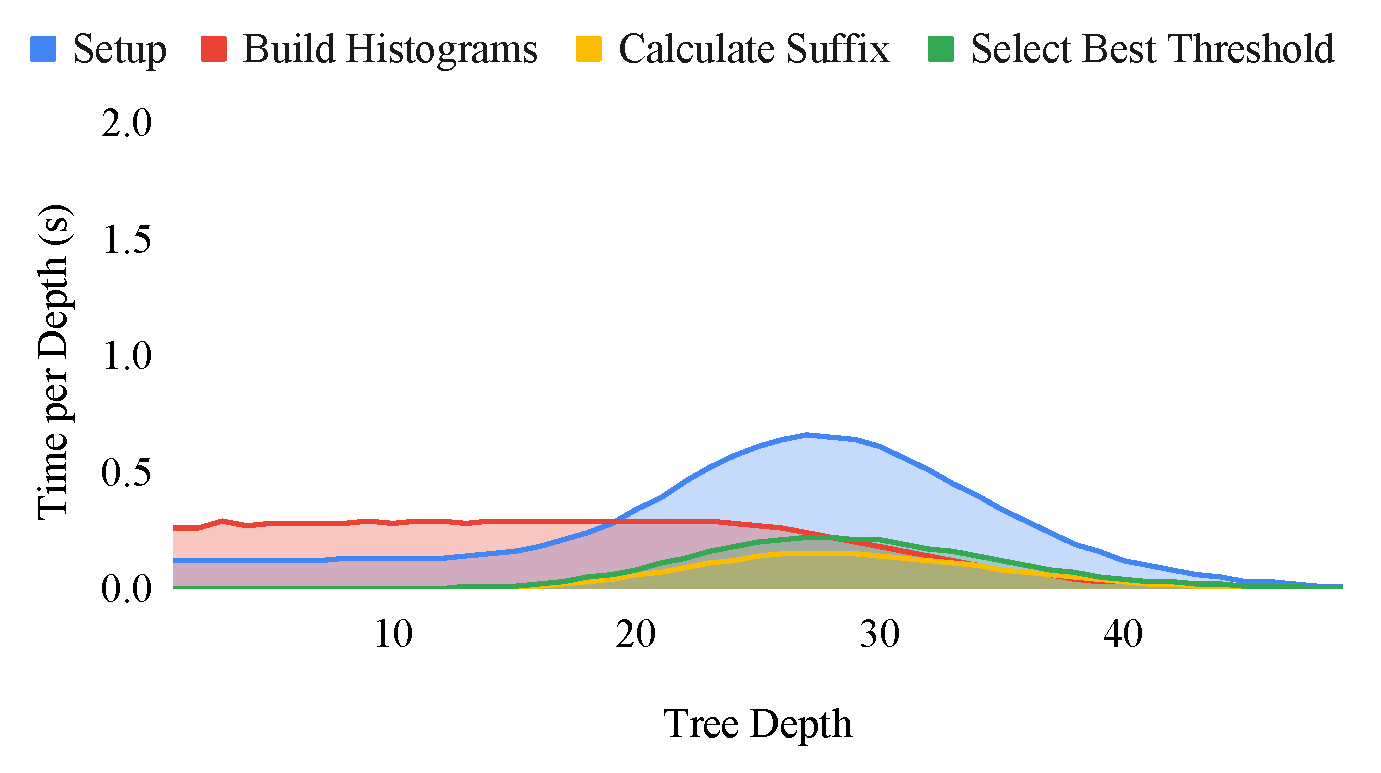
\includegraphics[width=\linewidth]{figures/results/vectorized/why-AVX-512-is-slower-high-depth/AVX2.pdf}
\caption{AVX2 (64 bins)}
\end{subfigure}
\hfill
\begin{subfigure}[b]{0.49\textwidth}
\centering
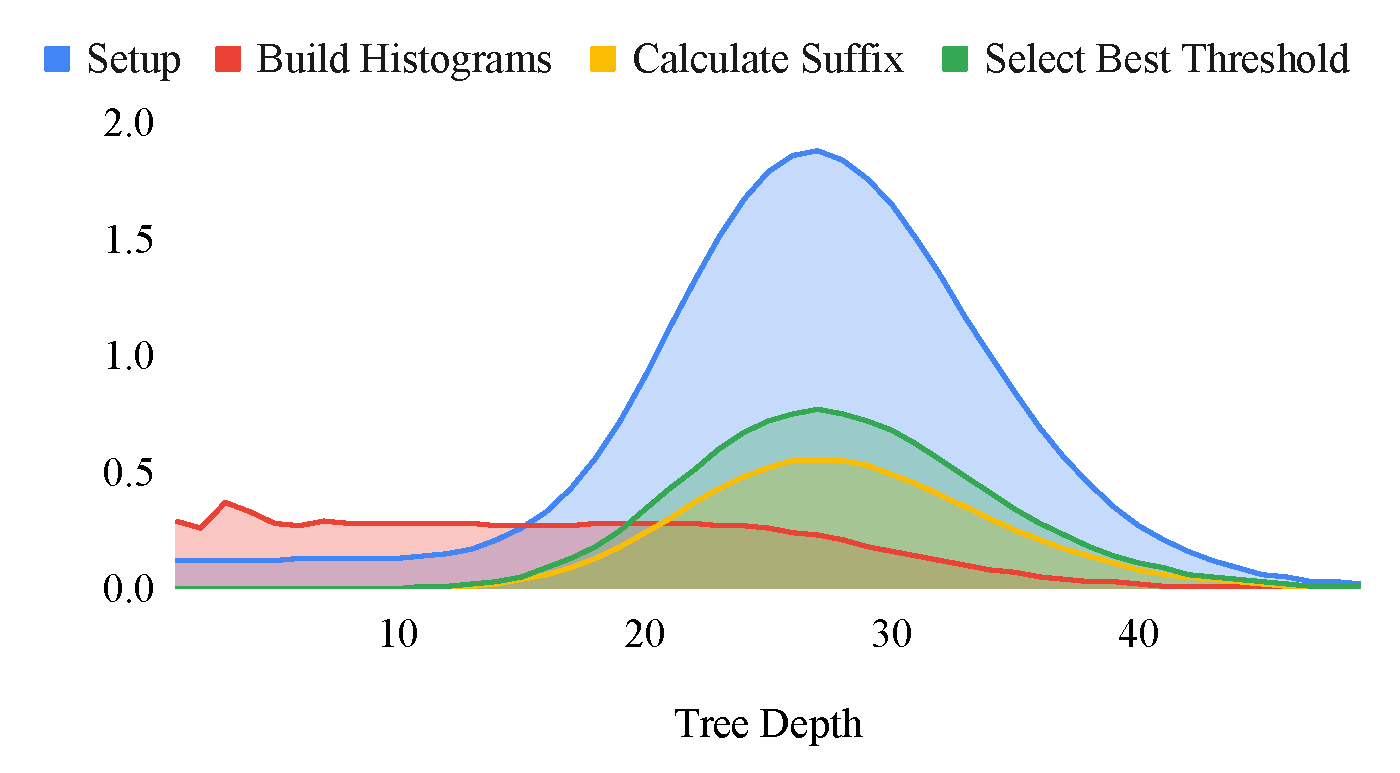
\includegraphics[width=\linewidth]{figures/results/vectorized/why-AVX-512-is-slower-high-depth/AVX-512.pdf}
\caption{AVX-512 (256 bins)}
\end{subfigure}
\caption{Vectorized histogram cost breakdown: AVX2 with 64 bins (left) and AVX-512 with 256 bins (right).}
\label{fig:AVX-512-slower}
\Description{Side-by-side cost breakdown of the vectorized histogram split finder with AVX2 at 64 bins and AVX-512 at 256 bins.}
\end{figure*}

\subsection{Dynamic Threshold Sensitivity Study}
\label{app:threshold-sensitivity}

\begin{figure}[t]
    \centering
    % Generated by benchmarks/src/utils/make_breakeven_figure.py -- do not hand-edit.
\definecolor{brk0}{HTML}{4285F4}
\definecolor{brk1}{HTML}{EA4335}
\definecolor{brk2}{HTML}{FBBC05}
\definecolor{brk3}{HTML}{EDA100}
\definecolor{brk4}{HTML}{E87BA4}
\definecolor{brk5}{HTML}{008300}
\definecolor{brk6}{HTML}{34A853}
\begin{tikzpicture}
\begin{axis}[width=\linewidth, height=5.2cm, xmode=log, xmin=100, xmax=10000,
  ymin=1.05, ymax=1.36, xtick={100,200,500,1000,2000,5000,10000}, log ticks with fixed point,
  xlabel={Dynamic Switch Threshold},
  ylabel={Speedup over Exact}, tick label style={font=\scriptsize},
  label style={font=\scriptsize}, grid=none, axis line style={gray!60}, tick style={draw=none},
  every axis plot/.append style={line width=0.7pt, mark size=1.1pt},
  legend style={font=\scriptsize, draw=none, fill=none, at={(0.5,1.02)}, anchor=south, legend columns=3,
    /tikz/every even column/.append style={column sep=4pt}}, legend cell align=left,
  scaled y ticks=false, yticklabel style={/pgf/number format/fixed, /pgf/number format/precision=2}]
\fill[gray!14] (axis cs:800,1.05) rectangle (axis cs:1200,1.36);
\fill[gray!30] (axis cs:300,1.05) rectangle (axis cs:500,1.36);
\addplot[gray!70, dashed, line width=0.6pt, forget plot] coordinates {(100,1) (10000,1)};
\addplot[color=brk0, mark=none, solid, forget plot] coordinates {(100,1.1750) (200,1.2216) (300,1.2491) (400,1.2501) (500,1.2514) (600,1.2515) (700,1.2535) (800,1.2544) (900,1.2547) (1000,1.2523) (1200,1.2563) (1400,1.2546) (1600,1.2534) (1800,1.2496) (2000,1.2466) (2500,1.2471) (3000,1.2427) (3500,1.2390) (4000,1.2319) (4500,1.2313) (5000,1.2311) (6000,1.2328) (7000,1.2304) (8000,1.2195) (9000,1.2305) (10000,1.2257)};
\addplot[color=black, mark=x, mark size=2.6pt, only marks, forget plot] coordinates {(1200,1.2563)};
\addplot[color=brk1, mark=none, solid, forget plot] coordinates {(100,1.2072) (200,1.2639) (300,1.2808) (400,1.2819) (500,1.2978) (600,1.2987) (700,1.2998) (800,1.3006) (900,1.2956) (1000,1.2990) (1200,1.2912) (1400,1.2951) (1600,1.2929) (1800,1.2906) (2000,1.2891) (2500,1.2805) (3000,1.2786) (3500,1.2731) (4000,1.2714) (4500,1.2721) (5000,1.2695) (6000,1.2630) (7000,1.2564) (8000,1.2532) (9000,1.2411) (10000,1.2480)};
\addplot[color=black, mark=x, mark size=2.6pt, only marks, forget plot] coordinates {(800,1.3006)};
\addplot[color=brk2, mark=none, solid, forget plot] coordinates {(100,1.0690) (200,1.1397) (300,1.1691) (400,1.1758) (500,1.1836) (600,1.1875) (700,1.1900) (800,1.1877) (900,1.1943) (1000,1.1931) (1200,1.1873) (1400,1.1918) (1600,1.1853) (1800,1.1842) (2000,1.1821) (2500,1.1620) (3000,1.1550) (3500,1.1751) (4000,1.1712) (4500,1.1633) (5000,1.1663) (6000,1.1609) (7000,1.1578) (8000,1.1536) (9000,1.1527) (10000,1.1501)};
\addplot[color=black, mark=x, mark size=2.6pt, only marks, forget plot] coordinates {(900,1.1943)};
\addplot[color=brk6, mark=none, solid, forget plot] coordinates {(100,1.2589) (200,1.2890) (300,1.3010) (400,1.3129) (500,1.3131) (600,1.3150) (700,1.3125) (800,1.3187) (900,1.3205) (1000,1.3085) (1200,1.3160) (1400,1.3053) (1600,1.3077) (1800,1.3068) (2000,1.3009) (2500,1.2978) (3000,1.2940) (3500,1.2923) (4000,1.2914) (4500,1.2884) (5000,1.2863) (6000,1.2873) (7000,1.2785) (8000,1.2742) (9000,1.2741) (10000,1.2698)};
\addplot[color=black, mark=x, mark size=2.6pt, only marks, forget plot] coordinates {(900,1.3205)};
\addplot[color=brk0, mark=none, dash pattern=on 2pt off 1.5pt, forget plot] coordinates {(100,1.2521) (200,1.2671) (300,1.2742) (400,1.2745) (500,1.2701) (600,1.2676) (700,1.2616) (800,1.2672) (900,1.2641) (1000,1.2571) (1200,1.2598) (1400,1.2553) (1600,1.2491) (1800,1.2473) (2000,1.2481) (2500,1.2398) (3000,1.2362) (3500,1.2364) (4000,1.2321) (4500,1.2270) (5000,1.2330) (6000,1.2240) (7000,1.2232) (8000,1.2200) (9000,1.2256) (10000,1.2168)};
\addplot[color=black, mark=x, mark size=2.6pt, only marks, forget plot] coordinates {(400,1.2745)};
\addplot[color=brk1, mark=none, dash pattern=on 2pt off 1.5pt, forget plot] coordinates {(100,1.3136) (200,1.3289) (300,1.3359) (400,1.3319) (500,1.3281) (600,1.3254) (700,1.3105) (800,1.3166) (900,1.3117) (1000,1.3149) (1200,1.3056) (1400,1.3005) (1600,1.3012) (1800,1.3005) (2000,1.2943) (2500,1.2891) (3000,1.2805) (3500,1.2784) (4000,1.2750) (4500,1.2648) (5000,1.2601) (6000,1.2601) (7000,1.2555) (8000,1.2485) (9000,1.2468) (10000,1.2487)};
\addplot[color=black, mark=x, mark size=2.6pt, only marks, forget plot] coordinates {(300,1.3359)};
\addplot[color=brk2, mark=none, dash pattern=on 2pt off 1.5pt, forget plot] coordinates {(100,1.1960) (200,1.2175) (300,1.2212) (400,1.2237) (500,1.2208) (600,1.2148) (700,1.2163) (800,1.2086) (900,1.2059) (1000,1.2052) (1200,1.2017) (1400,1.1947) (1600,1.1931) (1800,1.1941) (2000,1.1852) (2500,1.1832) (3000,1.1818) (3500,1.1737) (4000,1.1658) (4500,1.1727) (5000,1.1657) (6000,1.1632) (7000,1.1583) (8000,1.1540) (9000,1.1513) (10000,1.1481)};
\addplot[color=black, mark=x, mark size=2.6pt, only marks, forget plot] coordinates {(400,1.2237)};
\addplot[color=brk6, mark=none, dash pattern=on 2pt off 1.5pt, forget plot] coordinates {(100,1.3162) (200,1.3314) (300,1.3233) (400,1.3267) (500,1.3317) (600,1.3250) (700,1.3244) (800,1.3223) (900,1.3251) (1000,1.3248) (1200,1.3161) (1400,1.3107) (1600,1.3210) (1800,1.3214) (2000,1.3091) (2500,1.3052) (3000,1.2974) (3500,1.2988) (4000,1.2925) (4500,1.2925) (5000,1.2955) (6000,1.2911) (7000,1.2774) (8000,1.2832) (9000,1.2824) (10000,1.2781)};
\addplot[color=black, mark=x, mark size=2.6pt, only marks, forget plot] coordinates {(500,1.3317)};
\addlegendimage{color=brk0, solid, line width=0.7pt, mark=none}
\addlegendentry{HIGGS}
\addlegendimage{color=brk1, solid, line width=0.7pt, mark=none}
\addlegendentry{SUSY}
\addlegendimage{color=black, dash pattern=on 2pt off 1.5pt, line width=0.7pt, mark=none}
\addlegendentry{AVX2}
\addlegendimage{color=brk2, solid, line width=0.7pt, mark=none}
\addlegendentry{Epsilon}
\addlegendimage{color=brk6, solid, line width=0.7pt, mark=none}
\addlegendentry{YouTube-8M}
\addlegendimage{color=black, solid, line width=0.7pt, mark=none}
\addlegendentry{AVX-512}
\end{axis}
\end{tikzpicture}

    \caption{Full-depth train speedup over Exact by a linesearch over Dynamic Thresholds. Above the threshold, Random-Vectorized is used, and below, Exact. Shaded bands: the range of the AVX-512 maxima (light, 800--1200 rows) and of the AVX2 maxima (dark, 300--500 rows).}
    \Description{Line chart of training speedup over all-exact against the switch threshold on a logarithmic axis from 100 to 10000 for four datasets and two vectorized binners, with an X marking each curve's maximum and two shaded bands marking the AVX-512 and AVX2 maxima ranges.}
    \label{fig:threshold-sensitivity}
\end{figure}

Figure~\ref{fig:threshold-sensitivity} varies the switch threshold $\tau$ from 100 to 10000 rows on HIGGS, SUSY, Epsilon and YouTube-8M at full depth. The optimum lies at 300--500 rows for AVX2 with 64 bins (1.22--1.34$\times$) and at 800--1200 rows for AVX-512 with 256 bins (1.19--1.32$\times$): the larger bin count raises the fixed cost per histogram and with it the node size at which a histogram beats a sort. The curves are flat. Every AVX2 curve stays within 2\% of its maximum between 200 and 1000 rows and every AVX-512 curve between 400 and 2500; pushing $\tau$ to 10000, which sorts all but the largest nodes, still retains 93--98\% of the best speedup, and $\tau=100$ costs 1--2\% (AVX2) and 5--10\% (AVX-512). The fixed values used throughout, $\tau=250$ (AVX2) and $\tau=1000$ (AVX-512), are within 1\% of every per-dataset optimum, so no per-machine tuning was needed for the results of this section. %The scalar 64-bin binner moves the breakeven to about 4600 rows (sweep not shown), which is why it is reported only in its all-histogram form. no, this threshold is >50k. dropped

% \subsection{\TODO{Roofline} Pre-Vec v. Vec (std::sort \& Random v. HWY \& Vec Random}

% AL add. Optionally add Roofline of May 2025

% auto-generated by analyze.py:make_paper_tables -- regenerate, do not hand-edit
\begin{table*}[t]
\centering
\footnotesize
\setlength{\tabcolsep}{2.2pt}
\caption{Training time comparison to popular libraries using GBT (Boosting) and Random Forests (bagging). These are not like-for-like comparisons (see footnote), but are included in expectation of high interest in such a comparison.}
% Important Ariel Sept-24-2026. Confirmed these numbers. XGboost says "XGBRFClassifier is deprecated and "does not implement a conventional random forest"
% LGBM runs single-threaded, parallelizes within a tree
\label{tab:train-time-vs-libraries}
\begin{tabular}{l|cc|cccc|cccc}
\hline
\multicolumn{11}{l}{\textit{Random Forest (full-depth)}} \\
\hline
\multirow{3}{*}{\textbf{Dataset}} & \multicolumn{2}{c|}{\textbf{SPO-RF Baselines}} & \multicolumn{4}{c|}{\textbf{SPO-RF Our Methods}} & \multicolumn{4}{c}{\textbf{Other RF}} \\
 & \textbf{Exact} & \textbf{Random Hist.} & \textbf{Vec. Random Hist.} & \textbf{Vec. Random Hist.} & \textbf{Vec. Dynamic Hist.} & \textbf{Vec. Dynamic Hist.} & \textbf{AA-RF} & \textbf{XGBoost}$^\dagger$ & \textbf{LightGBM}$^\dagger$ & \textbf{CatBoost}$^\dagger$ \\
 & \scriptsize HWY & \scriptsize scalar, 64 bins & \scriptsize AVX2, 64 bins & \scriptsize AVX-512, 256 bins & \scriptsize AVX2, 64 bins \& HWY & \scriptsize AVX-512, 256 bins \& HWY & \scriptsize Exact & \scriptsize RF mode & \scriptsize RF mode & \scriptsize RF mode \\
\hline
HIGGS & 363.0 & 524.2 & 382.3 & 560.1 & 296.2 & \textbf{287.5} & 292.4 & 3000.9 & 2598.8 & --- \\
SUSY & 119.6 & 171.3 & 119.4 & 175.6 & 91.8 & \textbf{90.2} & 104.3 & 1048.6 & 2281.1 & --- \\
Epsilon & 59.1 & 95.1 & 68.6 & 109.8 & \textbf{50.5} & 50.7 & 52.1 & OOM & OOM & --- \\
\hline
\end{tabular}
\par\vspace{6pt}
\begin{tabular}{l|cc|cccc|cccc}
\hline
\multicolumn{11}{l}{\textit{Gradient Boosted Trees (depth 6)}} \\
\hline
\multirow{3}{*}{\textbf{Dataset}} & \multicolumn{2}{c|}{\textbf{SPO-GBT Baselines}} & \multicolumn{4}{c|}{\textbf{SPO-GBT Our Methods}} & \multicolumn{4}{c}{\textbf{Other GBT}} \\
 & \textbf{Exact} & \textbf{Random Hist.} & \textbf{Vec. Random Hist.} & \textbf{Vec. Random Hist.} & \textbf{Vec. Dynamic Hist.} & \textbf{Vec. Dynamic Hist.} & \textbf{AA-GBT}$^*$ & \textbf{XGBoost}$^*$ & \textbf{LightGBM}$^*$ & \textbf{CatBoost}$^*$ \\
 & \scriptsize HWY & \scriptsize scalar, 64 bins & \scriptsize AVX2, 64 bins & \scriptsize AVX-512, 256 bins & \scriptsize AVX2, 64 bins \& HWY & \scriptsize AVX-512, 256 bins \& HWY & \scriptsize Exact & \scriptsize  & \scriptsize  & \scriptsize  \\
\hline
HIGGS & 1617.9 & 2519.0 & 1242.3 & 1225.8 & --- & --- & 746.6 & 21.8 & \textbf{18.2} & 35.9 \\
SUSY & 638.2 & 896.7 & 460.7 & 437.9 & --- & --- & 267.6 & 7.1 & \textbf{6.1} & 14.7 \\
Epsilon & 96.6 & 159.4 & 75.2 & 74.8 & --- & --- & 490.0 & 56.1 & 52.7 & \textbf{24.0} \\
\hline
\end{tabular}
\\[2pt]
\parbox{0.92\linewidth}{\footnotesize $^\dagger$ RF implementations of this method are not directly comparable. XGBoost 3.4.1 warns that \texttt{XGBRFClassifier} is deprecated and ``does not implement a conventional random forest'', and LightGBM only parallelizes within a tree, similar to YDF-GBT, even in Random Forest mode. This explains the slow performance of the two methods. CatBoost does not support Random Forest (Bagged) mode.\\
$^*$ These methods benefit from features being fixed throughout training (no random projections), and can use optimizations like pre-sorting. It is unclear to us why YDF's AA-GBT does not benefit to a similar extent.}
\end{table*}


% tab:train-time-vs-libraries is input from comparison_with_libraries.tex, next to the
% Training time discussion; these two are accuracy only.
% Dropped 2026-09-09 (user request): mean accuracy/AUC + mean-rank suite table.
%% auto-generated by analyze.py:make_paper_tables -- regenerate, do not hand-edit
\begin{table*}[t]
\centering
\small
\caption{Mean accuracy/AUC and mean AUC rank (within family) -- all suite datasets; training time is in Table~\ref{tab:train-time-vs-libraries}. Bold: best value per column within each family.}
\label{tab:auc-vs-libraries-summary}
\begin{tabular}{lrrrr}
\toprule
Method & $n$ & Mean AUC & Mean acc. & Mean rank (AUC) \\
\midrule
SPO-RF Exact (std::sort) & 33 & 0.8301 & 0.8645 & 6.48 \\
SPO-RF Exact (Highway) & 33 & 0.8301 & 0.8645 & 6.48 \\
SPO-RF Random (scalar) & 33 & 0.8295 & 0.8646 & 5.74 \\
SPO-RF Random (vec) & 33 & 0.8295 & 0.8646 & 5.74 \\
SPO-RF Random-256 (AVX-512) & 33 & 0.8304 & \textbf{0.8649} & \textbf{4.82} \\
SPO-RF Dyn (scalar) & 33 & 0.8303 & 0.8645 & 5.30 \\
SPO-RF Dyn-Vec [ours] & 33 & 0.8299 & \textbf{0.8649} & 5.88 \\
SPO-RF Dyn-256 (AVX-512) & 33 & 0.8295 & 0.8643 & 6.48 \\
AA-RF Exact & 33 & 0.8281 & 0.8634 & 6.85 \\
XGBoost RF mode & 33 & \textbf{0.8356} & 0.8606 & 4.91 \\
LightGBM RF mode & 33 & 0.8272 & 0.8546 & 7.30 \\
\midrule
SPO-GBT Exact & 33 & 0.8311 & 0.8656 & 3.36 \\
SPO-GBT Dyn-Vec [ours] & 33 & 0.8289 & 0.8653 & 3.88 \\
SPO-GBT Dyn-256 (AVX-512) & 33 & 0.8299 & 0.8648 & 3.97 \\
AA-GBT Exact & 33 & 0.8275 & 0.8630 & 4.97 \\
XGBoost & 33 & 0.8284 & 0.8641 & 4.30 \\
LightGBM & 33 & 0.8252 & 0.8621 & 5.24 \\
CatBoost & 33 & \textbf{0.8334} & \textbf{0.8666} & \textbf{2.27} \\
\bottomrule
\end{tabular}
\end{table*}

% % auto-generated by analyze.py:make_paper_tables -- regenerate, do not hand-edit
\begin{table*}[t]
\centering
\small
\caption{Huge-dataset accuracy (single held-out split). Bold: best AUC/Acc.\ per dataset within each family. \TODO{Keep only table 3}}
\label{tab:auc-vs-libraries-large}
\begin{tabular*}{0.92\linewidth}{@{\extracolsep{\fill}}lcccccc}
\toprule
\multicolumn{1}{l}{} & \multicolumn{2}{c}{HIGGS} & \multicolumn{2}{c}{SUSY} & \multicolumn{2}{c}{EPSILON} \\
\cmidrule(lr){2-3} \cmidrule(lr){4-5} \cmidrule(lr){6-7}
Method & AUC & Acc. & AUC & Acc. & AUC & Acc. \\
\midrule
SPO-RF Exact (std::sort) & 0.8472 & 0.7619 & 0.8746 & 0.8021 & 0.8602 & 0.7778 \\
SPO-RF Exact (Highway) & 0.8472 & 0.7619 & 0.8746 & 0.8021 & 0.8602 & 0.7778 \\
SPO-RF Random (scalar) & 0.8472 & 0.7617 & 0.8746 & 0.8022 & 0.8569 & 0.7744 \\
SPO-RF Random (vec) & 0.8472 & 0.7617 & 0.8746 & 0.8022 & 0.8569 & 0.7744 \\
SPO-RF Random-256 (AVX-512) & 0.8472 & 0.7622 & 0.8747 & 0.8022 & 0.8585 & 0.7758 \\
SPO-RF Dyn (scalar) & 0.8473 & 0.7616 & 0.8748 & 0.8022 & 0.8585 & 0.7754 \\
SPO-RF Dyn-Vec [ours] & 0.8472 & 0.7617 & 0.8745 & 0.8021 & 0.8568 & 0.7748 \\
SPO-RF Dyn-256 (AVX-512) & 0.8472 & 0.7618 & 0.8745 & 0.8018 & 0.8574 & 0.7745 \\
AA-RF Exact & \textbf{0.8487} & \textbf{0.7632} & 0.8740 & 0.8016 & \textbf{0.8651} & \textbf{0.7832} \\
XGBoost RF mode & 0.8428 & 0.7598 & \textbf{0.8754} & \textbf{0.8023} & \multicolumn{2}{c}{OOM} \\
LightGBM RF mode & 0.8301 & 0.7489 & 0.8752 & \textbf{0.8023} & \multicolumn{2}{c}{OOM} \\
\midrule
SPO-GBT Exact & 0.8123 & 0.7323 & 0.8769 & 0.8031 & 0.9348 & 0.8572 \\
SPO-GBT Dyn-Vec [ours] & 0.8104 & 0.7306 & 0.8767 & 0.8027 & 0.9350 & 0.8584 \\
SPO-GBT Dyn-256 (AVX-512) & 0.8120 & 0.7317 & 0.8770 & 0.8035 & 0.9348 & 0.8578 \\
AA-GBT Exact & 0.8197 & 0.7382 & 0.8774 & 0.8037 & 0.9403 & 0.8655 \\
XGBoost & \textbf{0.8251} & \textbf{0.7430} & \textbf{0.8779} & \textbf{0.8039} & \textbf{0.9428} & 0.8683 \\
LightGBM & 0.8250 & 0.7428 & 0.8776 & 0.8036 & 0.9426 & 0.8677 \\
CatBoost & 0.8159 & 0.7354 & 0.8771 & 0.8036 & 0.9424 & \textbf{0.8694} \\
\bottomrule
\end{tabular*}
\\[2pt]
\parbox{0.92\linewidth}{\footnotesize \TODO{Histogram bin counts are not matched across libraries} (SPO-RF/SPO-GBT: 64; XGBoost: 256; LightGBM: 255; CatBoost: 254), disclosed rather than hidden. CatBoost's bootstrap is disabled; no arm uses class weighting.}
\end{table*}


% \FloatBarrier
\subsection{Accuracy}
\label{sec:res-accuracy}

\TODO{SPO-GBT mistakenly used $\sqrt{\mathbf{F}}$ projections instead of $\mathbf{F}$, putting it at an unfair disadvantage}

Vectorization changes no model: the scalar and vectorized binners bin identically and produce identical forests, which is why their accuracy columns coincide in Table~\ref{tab:auc-vs-libraries-per-dataset-auc}. The dynamic switch does change the model, since nodes below $\tau$ take an exact split where an all-histogram forest would take a binned one. Table~\ref{tab:hist-vs-exact-summary} measures the effect on held-out accuracy against Exact on 34 OpenML CC18 binary tasks (10-fold cross-validation $\times$ 3 seeds) plus HIGGS and SUSY. For SPO-RF the mean difference of the dynamic forest to Exact is $+5\times10^{-3}$ with a 95\% interval of $[-4, +14]\times10^{-3}$ that includes zero; it wins on 13 datasets, ties on 17 and loses on 6, and only two per-dataset differences survive Holm correction. For SPO-GBT the difference is $+1\times10^{-3}$ $[-1, +3]$ (9 wins, 20 ties, 7 losses), with electricity and adult significantly below Exact by 1.6 and 0.1 points. The dynamic forests are non-inferior to Exact within $2.5\times10^{-3}$ (RF) and $1\times10^{-3}$ (GBT) accuracy at $\alpha=0.05$, and the all-histogram forests fall in the same intervals. On the large datasets the SPO-RF finders agree to three decimals (HIGGS 0.762 and SUSY 0.802 for Exact and Dynamic alike) and the SPO-GBT ones within 0.2 points. Against XGBoost, LightGBM, CatBoost and axis-aligned YDF (Table ~\ref{tab:train-time-vs-libraries}, ~\ref{tab:auc-vs-libraries-per-dataset-auc}), the RF and GBT learners are very similar, and the dynamic vectorized configuration ties the exact baseline on 34 of 36 datasets.

% % ---------------------------------------------------------------------------
% Comparison with axis-aligned learners (XGBoost, LightGBM, CatBoost) and the
% speedup map. Numbers come from benchmarks/results/spo_vs_gbt/ (drivers in
% benchmarks/evaluation/spo_vs_gbt/, protocol in /home/ubuntu/spo_vs_gbt/PROTOCOL.md).
% Tables tables/table_{train_time,auc}_vs_libraries*.tex and figures figures/results/spo_vs_gbt_* are
% generated by analyze.py -- regenerate, never hand-edit.
% ---------------------------------------------------------------------------
\subsection{Accuracy Comparison with XGBoost, LightGBM and CatBoost}
\label{sec:spo-vs-gbt}

\textbf{\textit{Claude wrote this}}

We compare our shipped configuration (dynamic histogram/exact switching with vectorized
binning, ``SPO Dyn-Vec'') against the SPO exact baseline (\texttt{std::sort} or Highway's
vectorized sort), YDF's axis-aligned learners, and XGBoost, LightGBM and CatBoost, for RF and
GBT.

\paragraph{Protocol.}
RF: 240 fully grown trees, bootstrap sampling, $\sqrt{F}$ candidate features or projections per
node. GBT: 300 trees of depth~6, learning rate~0.1, no subsampling or early stopping, default
bin counts. Datasets: the 30 binary TabArena-v0.1 tasks~\cite{tabarena} (748--150k rows,
4--1776 features) under stratified 5-fold cross-validation, three TabReD~\cite{tabred}
classification sets on their chronological 80/20 holdout, and HIGGS, SUSY and Epsilon on a
single held-out split; categoricals are ordinal-encoded, missing values training-fold-mean
imputed. ROC AUC is the primary metric, compared by mean rank (Friedman and Nemenyi tests) and
by Holm-corrected Wilcoxon signed-rank tests of SPO Dyn-Vec against each competitor, with
$|\Delta\mathrm{AUC}|<0.005$ counted as a tie.

% Accuracy sensitivity analysis
% \begin{figure}[t]
%     \centering
%     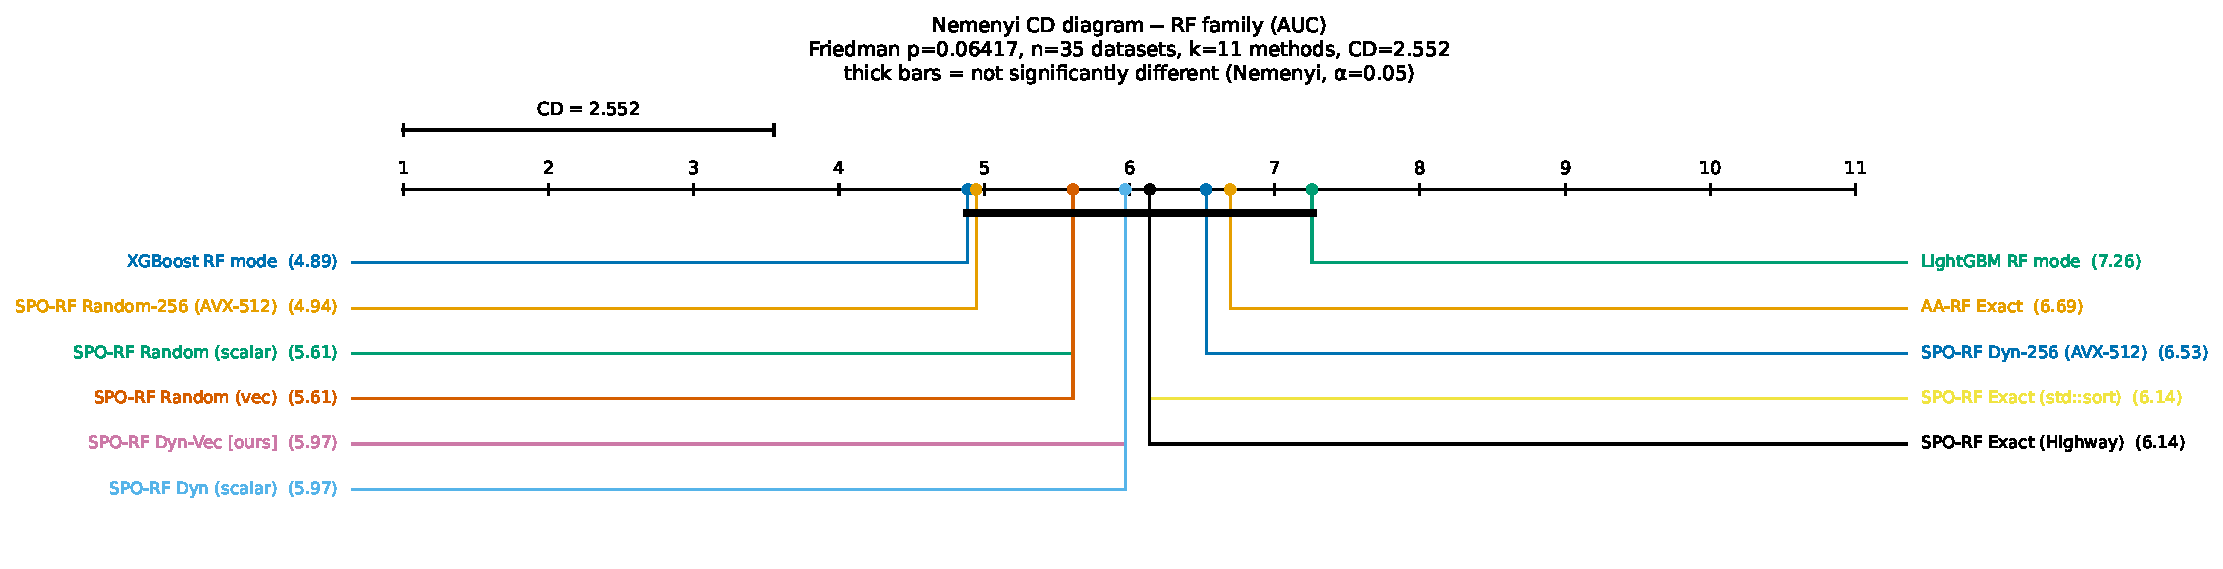
\includegraphics[width=\linewidth]{figures/results/spo_vs_gbt_cd_rf_auc.pdf}\\[4pt]
%     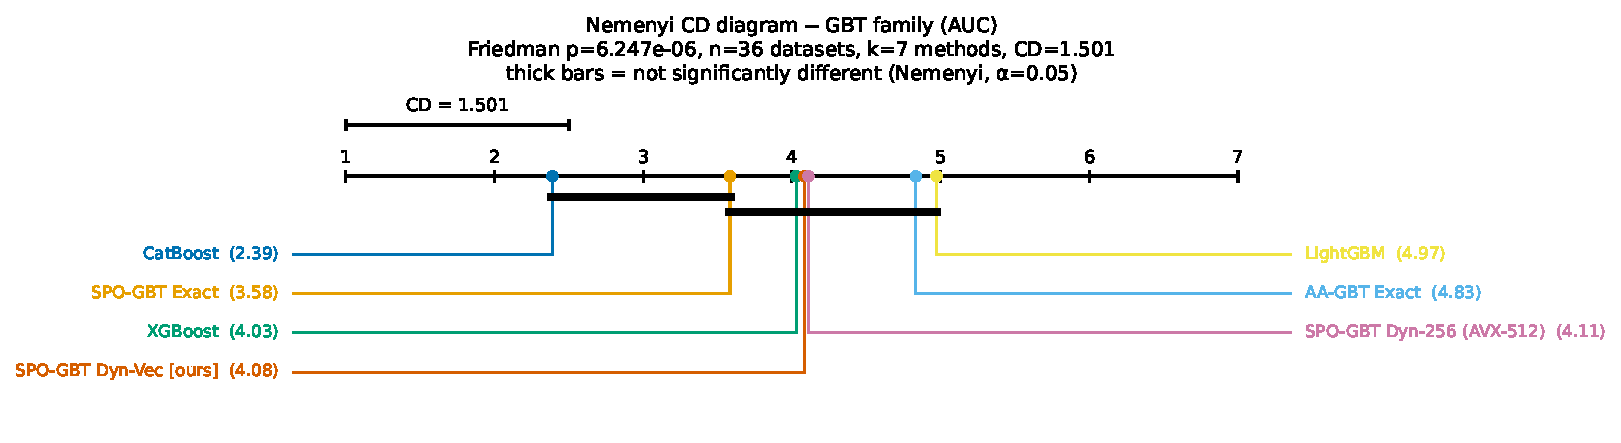
\includegraphics[width=\linewidth]{figures/results/spo_vs_gbt_cd_gbt_auc.pdf}
%     \caption{Nemenyi critical-difference diagrams of mean AUC rank over the TabArena/TabReD suite
%     and the three large datasets, RF family (top) and GBT family (bottom). Methods joined by a
%     thick bar are not significantly different ($\alpha=0.05$).}
%     \Description{Two critical-difference diagrams.}
%     \label{fig:spo-vs-gbt-cd}
% \end{figure}

\paragraph{Accuracy.}
(Table~\ref{tab:auc-vs-libraries-summary}, Figure~\ref{fig:spo-vs-gbt-cd}.) The RF learners are
statistically indistinguishable (Friedman $p=0.06$); SPO Dyn-Vec ties the exact baseline on 34
of 36 datasets. Among GBTs CatBoost ranks first (Friedman $p=6\times10^{-6}$), but no pairwise
comparison against SPO Dyn-Vec survives Holm correction. On HIGGS SPO Dyn-Vec RF reaches AUC
0.847 versus 0.843 (XGBoost-RF) and 0.830 (LightGBM-RF); both library RF modes run out of
memory on Epsilon (Table~\ref{tab:auc-vs-libraries-large}). Sparse oblique splits are as accurate as
the best axis-aligned learners here, not better; 256 bins instead of 64 changes neither time
($0.98\times$) nor any conclusion.

% all runtime numbers, split out of the accuracy tables (analyze.py)
% auto-generated by analyze.py:make_paper_tables -- regenerate, do not hand-edit
\begin{table*}[t]
\centering
\footnotesize
\setlength{\tabcolsep}{2.2pt}
\caption{Training time comparison to popular libraries using GBT (Boosting) and Random Forests (bagging). These are not like-for-like comparisons (see footnote), but are included in expectation of high interest in such a comparison.}
% Important Ariel Sept-24-2026. Confirmed these numbers. XGboost says "XGBRFClassifier is deprecated and "does not implement a conventional random forest"
% LGBM runs single-threaded, parallelizes within a tree
\label{tab:train-time-vs-libraries}
\begin{tabular}{l|cc|cccc|cccc}
\hline
\multicolumn{11}{l}{\textit{Random Forest (full-depth)}} \\
\hline
\multirow{3}{*}{\textbf{Dataset}} & \multicolumn{2}{c|}{\textbf{SPO-RF Baselines}} & \multicolumn{4}{c|}{\textbf{SPO-RF Our Methods}} & \multicolumn{4}{c}{\textbf{Other RF}} \\
 & \textbf{Exact} & \textbf{Random Hist.} & \textbf{Vec. Random Hist.} & \textbf{Vec. Random Hist.} & \textbf{Vec. Dynamic Hist.} & \textbf{Vec. Dynamic Hist.} & \textbf{AA-RF} & \textbf{XGBoost}$^\dagger$ & \textbf{LightGBM}$^\dagger$ & \textbf{CatBoost}$^\dagger$ \\
 & \scriptsize HWY & \scriptsize scalar, 64 bins & \scriptsize AVX2, 64 bins & \scriptsize AVX-512, 256 bins & \scriptsize AVX2, 64 bins \& HWY & \scriptsize AVX-512, 256 bins \& HWY & \scriptsize Exact & \scriptsize RF mode & \scriptsize RF mode & \scriptsize RF mode \\
\hline
HIGGS & 363.0 & 524.2 & 382.3 & 560.1 & 296.2 & \textbf{287.5} & 292.4 & 3000.9 & 2598.8 & --- \\
SUSY & 119.6 & 171.3 & 119.4 & 175.6 & 91.8 & \textbf{90.2} & 104.3 & 1048.6 & 2281.1 & --- \\
Epsilon & 59.1 & 95.1 & 68.6 & 109.8 & \textbf{50.5} & 50.7 & 52.1 & OOM & OOM & --- \\
\hline
\end{tabular}
\par\vspace{6pt}
\begin{tabular}{l|cc|cccc|cccc}
\hline
\multicolumn{11}{l}{\textit{Gradient Boosted Trees (depth 6)}} \\
\hline
\multirow{3}{*}{\textbf{Dataset}} & \multicolumn{2}{c|}{\textbf{SPO-GBT Baselines}} & \multicolumn{4}{c|}{\textbf{SPO-GBT Our Methods}} & \multicolumn{4}{c}{\textbf{Other GBT}} \\
 & \textbf{Exact} & \textbf{Random Hist.} & \textbf{Vec. Random Hist.} & \textbf{Vec. Random Hist.} & \textbf{Vec. Dynamic Hist.} & \textbf{Vec. Dynamic Hist.} & \textbf{AA-GBT}$^*$ & \textbf{XGBoost}$^*$ & \textbf{LightGBM}$^*$ & \textbf{CatBoost}$^*$ \\
 & \scriptsize HWY & \scriptsize scalar, 64 bins & \scriptsize AVX2, 64 bins & \scriptsize AVX-512, 256 bins & \scriptsize AVX2, 64 bins \& HWY & \scriptsize AVX-512, 256 bins \& HWY & \scriptsize Exact & \scriptsize  & \scriptsize  & \scriptsize  \\
\hline
HIGGS & 1617.9 & 2519.0 & 1242.3 & 1225.8 & --- & --- & 746.6 & 21.8 & \textbf{18.2} & 35.9 \\
SUSY & 638.2 & 896.7 & 460.7 & 437.9 & --- & --- & 267.6 & 7.1 & \textbf{6.1} & 14.7 \\
Epsilon & 96.6 & 159.4 & 75.2 & 74.8 & --- & --- & 490.0 & 56.1 & 52.7 & \textbf{24.0} \\
\hline
\end{tabular}
\\[2pt]
\parbox{0.92\linewidth}{\footnotesize $^\dagger$ RF implementations of this method are not directly comparable. XGBoost 3.4.1 warns that \texttt{XGBRFClassifier} is deprecated and ``does not implement a conventional random forest'', and LightGBM only parallelizes within a tree, similar to YDF-GBT, even in Random Forest mode. This explains the slow performance of the two methods. CatBoost does not support Random Forest (Bagged) mode.\\
$^*$ These methods benefit from features being fixed throughout training (no random projections), and can use optimizations like pre-sorting. It is unclear to us why YDF's AA-GBT does not benefit to a similar extent.}
\end{table*}


\paragraph{Training time.}
(Table~\ref{tab:train-time-vs-libraries}.) For RF, SPO goes from slowest to fastest: on HIGGS the
exact baseline needs 719\,s, SPO Dyn-Vec 296\,s, axis-aligned YDF RF 292\,s, XGBoost-RF
3001\,s and LightGBM-RF 2599\,s. For depth-6 GBT the reverse holds: XGBoost and LightGBM train
HIGGS in 18--22\,s against 1242\,s for SPO-GBT Dyn-Vec, because shallow trees over millions of
rows are dominated by histogram construction and the dynamic switch never fires; on the wide
Epsilon the gap closes (75\,s vs.\ 53--56\,s). Per-dataset results are in
Tables~\ref{tab:auc-vs-libraries-per-dataset-rf-auc}--\ref{tab:auc-vs-libraries-per-dataset-gbt-time}.
XGBoost thus suffices for shallow boosted trees, where SPO has no accuracy advantage and we
claim none; for fully grown sparse oblique forests the libraries' RF modes are an order of
magnitude slower on large datasets and fail outright on wide ones, whereas our optimizations
bring SPO-RF to axis-aligned RF training time at equal or better accuracy.

% \begin{figure*}[t]
%     \centering
%     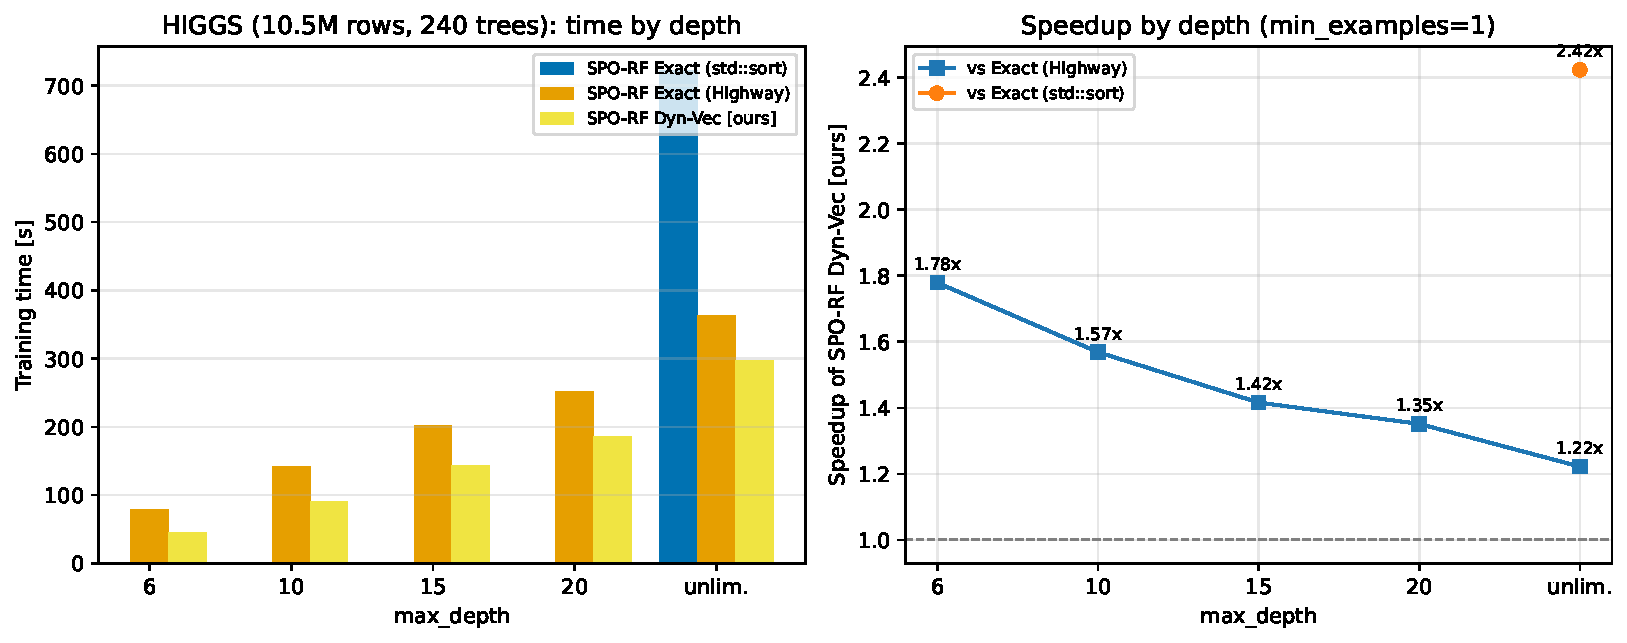
\includegraphics[width=0.60\linewidth]{figures/results/spo_vs_gbt_speedup_vs_depth.pdf}\hfill
%     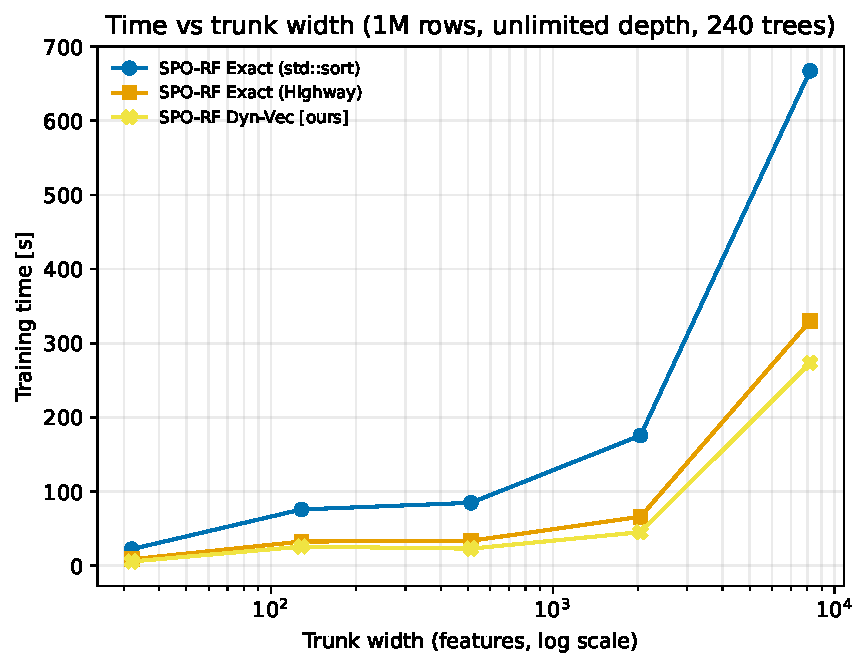
\includegraphics[width=0.305\linewidth]{figures/results/spo_vs_gbt_trunk_width.pdf}%\\[4pt]
%     % 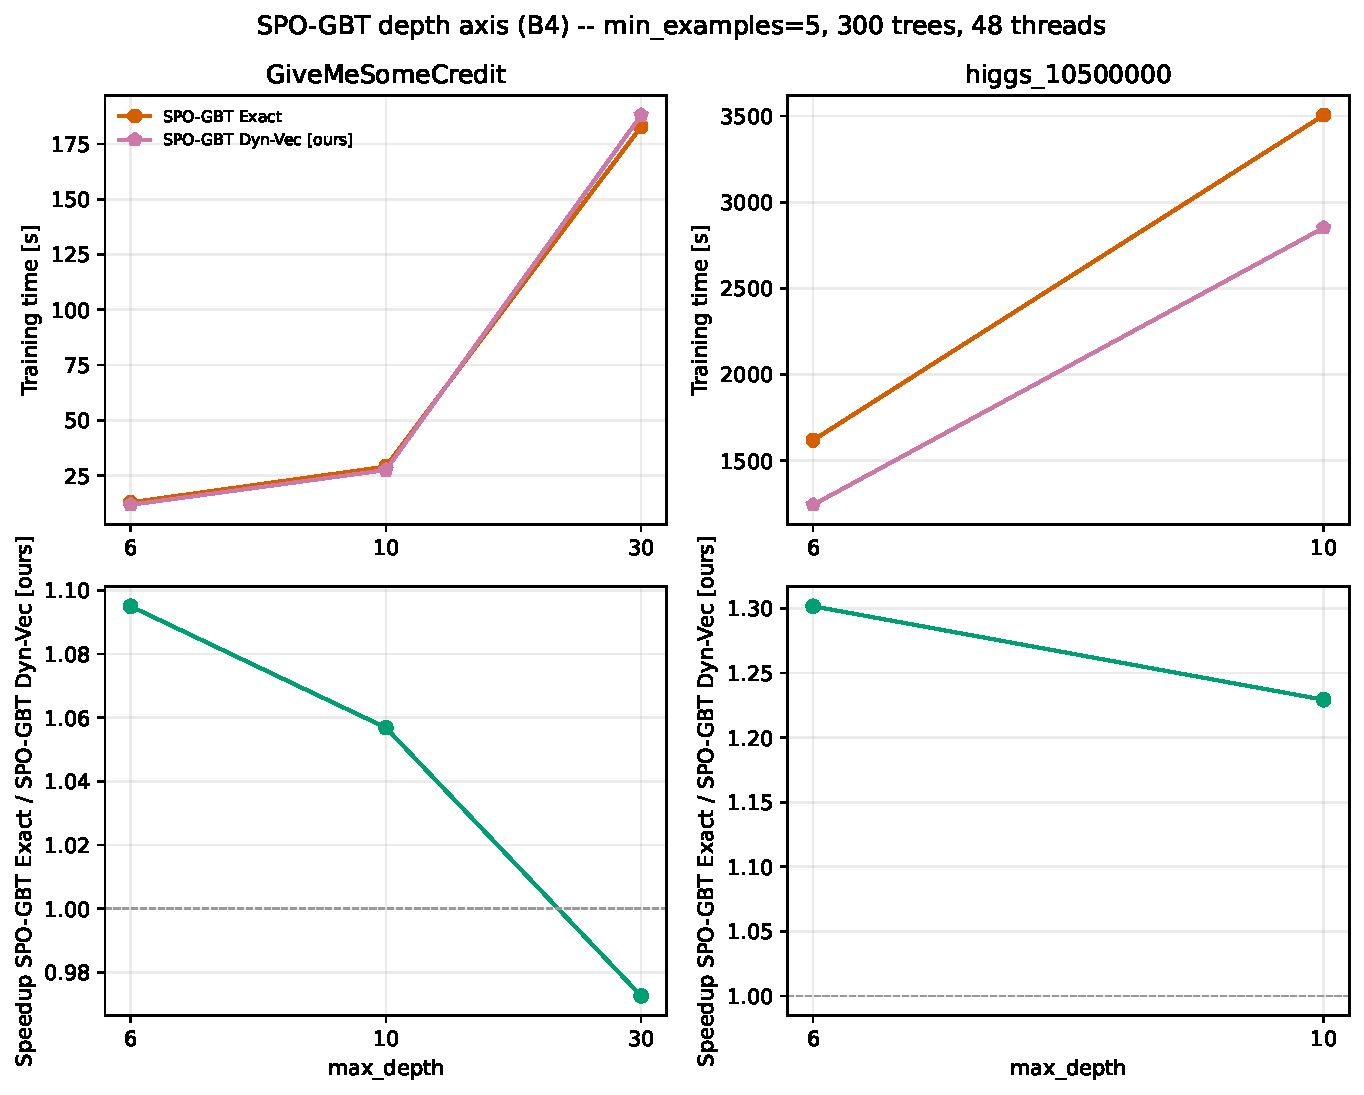
\includegraphics[width=0.62\linewidth]{figures/results/spo_vs_gbt_gbt_depth.pdf}
%     \caption{Speedup map of SPO Dyn-Vec. Top left: HIGGS (10.5M rows) by maximum depth, against
%     exact splitting with Highway's sort and with \texttt{std::sort}. Top right: training time on
%     Trunk with 1M rows by feature count. Bottom: SPO-GBT by depth.}
%     \Description{Three panels of training time and speedup along depth, width and boosting depth.}
%     \label{fig:speedup-map}
% \end{figure*}

\begin{figure*}[t]
    \centering
    % Generated by benchmarks/src/spo_vs_gbt/make_rowcol_map_depths.py -- regenerate, never hand-edit.
    % Generated by benchmarks/src/spaa27_experiments/make_rowcol_map_depths.py -- do not hand-edit.
% Needs \usepackage{pgfplots}\pgfplotsset{compat=1.18}\usepgfplotslibrary{groupplots}.
% Background: inverse-distance-weighted speedup (3 nearest points, log-log), see idw_field().
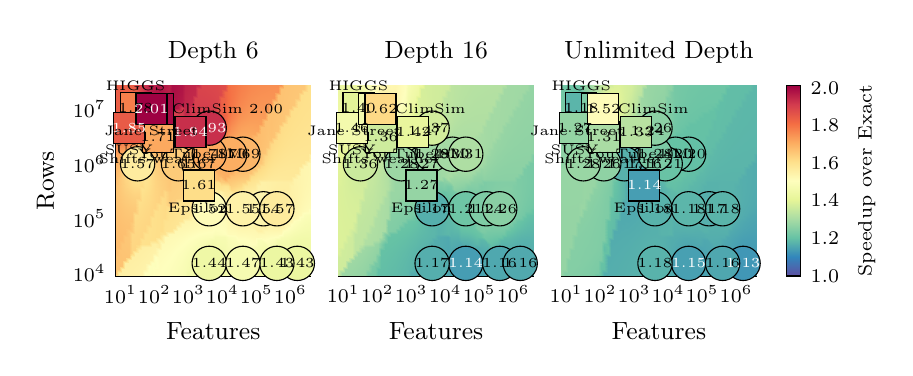
\begin{tikzpicture}
\pgfplotsset{
  colormap={spectralr}{rgb255(0cm)=(94,79,162); rgb255(1cm)=(50,134,188); rgb255(2cm)=(102,194,165); rgb255(3cm)=(169,220,164); rgb255(4cm)=(230,245,152); rgb255(5cm)=(254,254,189); rgb255(6cm)=(254,224,139); rgb255(7cm)=(252,172,96); rgb255(8cm)=(244,109,67); rgb255(9cm)=(211,60,78); rgb255(10cm)=(158,1,66)},
  rcmark/.style={scatter, only marks, scatter src=explicit,
    scatter/use mapped color={draw=black, fill=mapped color, line width=0.4pt}},
  rclabel/.style={only marks, mark=none, point meta=explicit, forget plot,
    nodes near coords={\pgfmathprintnumber[fixed,fixed zerofill,precision=2]{\pgfplotspointmeta}},
    nodes near coords style={font=\fontsize{4.2}{5}\selectfont, anchor=center, inner sep=0pt}},
  rcname/.style={only marks, mark=none, forget plot,
    visualization depends on={value \thisrow{name} \as \nm},
    nodes near coords={\nm}, nodes near coords style={font=\tiny, inner sep=1pt}},
}
\begin{groupplot}[
  group style={group size=3 by 1, horizontal sep=0.35cm, ylabels at=edge left, yticklabels at=edge left},
  width=0.335\linewidth, height=0.33\linewidth, xmode=log, ymode=log,
  point meta min=1.0000, point meta max=2.0129,
  xmin=7.2, xmax=4e+06, ymin=8823.53, ymax=2.73e+07,
  xtick={1e1,1e2,1e3,1e4,1e5,1e6}, ytick={1e4,1e5,1e6,1e7},
  xlabel={Features}, ylabel={Rows}, label style={font=\small}, tick label style={font=\scriptsize},
  title style={font=\small, yshift=-3pt}, tick style={draw=none}, enlargelimits=false, clip=true,
]
\nextgroupplot[title={\strut Depth 6}]
\addplot[surf, shader=interp, point meta=explicit, mesh/rows=60, mesh/cols=60, forget plot] table[x=x, y=y, meta=z] {
x y z
7.2 8823.5 1.6117
9.0095 8823.5 1.5553
11.274 8823.5 1.5542
14.107 8823.5 1.5531
17.652 8823.5 1.5517
22.089 8823.5 1.5501
27.64 8823.5 1.5482
34.587 8823.5 1.5461
43.279 8823.5 1.5437
54.156 8823.5 1.5048
67.767 8823.5 1.5022
84.798 8823.5 1.4995
106.11 8823.5 1.5089
132.78 8823.5 1.5069
166.15 8823.5 1.5047
207.9 8823.5 1.5022
260.15 8823.5 1.4993
325.53 8823.5 1.4961
407.34 8823.5 1.4924
509.72 8823.5 1.4883
637.82 8823.5 1.4838
798.12 8823.5 1.4788
998.7 8823.5 1.4584
1249.7 8823.5 1.4560
1563.8 8823.5 1.4534
1956.8 8823.5 1.4509
2448.5 8823.5 1.4487
3063.9 8823.5 1.4471
3833.9 8823.5 1.4464
4797.5 8823.5 1.4469
6003.2 8823.5 1.4488
7511.9 8823.5 1.4522
9399.8 8823.5 1.4565
11762 8823.5 1.4612
14718 8823.5 1.4683
18417 8823.5 1.4719
23046 8823.5 1.4738
28838 8823.5 1.4696
36085 8823.5 1.4707
45154 8823.5 1.4706
56502 8823.5 1.4691
70702 8823.5 1.4723
88471 8823.5 1.4688
1.1071e+05 8823.5 1.4546
1.3853e+05 8823.5 1.4483
1.7334e+05 8823.5 1.4427
2.1691e+05 8823.5 1.4385
2.7142e+05 8823.5 1.4357
3.3963e+05 8823.5 1.4343
4.2499e+05 8823.5 1.4337
5.318e+05 8823.5 1.4336
6.6545e+05 8823.5 1.4335
8.3269e+05 8823.5 1.4375
1.042e+06 8823.5 1.4364
1.3038e+06 8823.5 1.4352
1.6315e+06 8823.5 1.4346
2.0415e+06 8823.5 1.4351
2.5546e+06 8823.5 1.4364
3.1966e+06 8823.5 1.4383
4e+06 8823.5 1.4404
7.2 10111 1.6679
9.0095 10111 1.5563
11.274 10111 1.5554
14.107 10111 1.5543
17.652 10111 1.5530
22.089 10111 1.5514
27.64 10111 1.5497
34.587 10111 1.5477
43.279 10111 1.5453
54.156 10111 1.5059
67.767 10111 1.5033
84.798 10111 1.5006
106.11 10111 1.5099
132.78 10111 1.5080
166.15 10111 1.5058
207.9 10111 1.5033
260.15 10111 1.5005
325.53 10111 1.4972
407.34 10111 1.4935
509.72 10111 1.4893
637.82 10111 1.4847
798.12 10111 1.4795
998.7 10111 1.4585
1249.7 10111 1.4559
1563.8 10111 1.4531
1956.8 10111 1.4503
2448.5 10111 1.4477
3063.9 10111 1.4458
3833.9 10111 1.4449
4797.5 10111 1.4454
6003.2 10111 1.4475
7511.9 10111 1.4511
9399.8 10111 1.4559
11762 10111 1.4611
14718 10111 1.4686
18417 10111 1.4722
23046 10111 1.4741
28838 10111 1.4709
36085 10111 1.4721
45154 10111 1.4720
56502 10111 1.4705
70702 10111 1.4728
88471 10111 1.4694
1.1071e+05 10111 1.4551
1.3853e+05 10111 1.4482
1.7334e+05 10111 1.4422
2.1691e+05 10111 1.4377
2.7142e+05 10111 1.4349
3.3963e+05 10111 1.4335
4.2499e+05 10111 1.4331
5.318e+05 10111 1.4332
6.6545e+05 10111 1.4369
8.3269e+05 10111 1.4370
1.042e+06 10111 1.4356
1.3038e+06 10111 1.4340
1.6315e+06 10111 1.4333
2.0415e+06 10111 1.4339
2.5546e+06 10111 1.4355
3.1966e+06 10111 1.4376
4e+06 10111 1.4400
7.2 11587 1.6675
9.0095 11587 1.6665
11.274 11587 1.5565
14.107 11587 1.5555
17.652 11587 1.5543
22.089 11587 1.5528
27.64 11587 1.5512
34.587 11587 1.5492
43.279 11587 1.5470
54.156 11587 1.5444
67.767 11587 1.5045
84.798 11587 1.5017
106.11 11587 1.5111
132.78 11587 1.5092
166.15 11587 1.5071
207.9 11587 1.5046
260.15 11587 1.5018
325.53 11587 1.4985
407.34 11587 1.4948
509.72 11587 1.4906
637.82 11587 1.4858
798.12 11587 1.4805
998.7 11587 1.4746
1249.7 11587 1.4560
1563.8 11587 1.4530
1956.8 11587 1.4499
2448.5 11587 1.4470
3063.9 11587 1.4448
3833.9 11587 1.4437
4797.5 11587 1.4441
6003.2 11587 1.4463
7511.9 11587 1.4503
9399.8 11587 1.4555
11762 11587 1.4610
14718 11587 1.4689
18417 11587 1.4726
23046 11587 1.4743
28838 11587 1.4747
36085 11587 1.4732
45154 11587 1.4731
56502 11587 1.4743
70702 11587 1.4733
88471 11587 1.4700
1.1071e+05 11587 1.4652
1.3853e+05 11587 1.4481
1.7334e+05 11587 1.4417
2.1691e+05 11587 1.4371
2.7142e+05 11587 1.4342
3.3963e+05 11587 1.4329
4.2499e+05 11587 1.4326
5.318e+05 11587 1.4348
6.6545e+05 11587 1.4365
8.3269e+05 11587 1.4367
1.042e+06 11587 1.4349
1.3038e+06 11587 1.4329
1.6315e+06 11587 1.4321
2.0415e+06 11587 1.4329
2.5546e+06 11587 1.4347
3.1966e+06 11587 1.4372
4e+06 11587 1.4398
7.2 13278 1.6671
9.0095 13278 1.6660
11.274 13278 1.6650
14.107 13278 1.5567
17.652 13278 1.5556
22.089 13278 1.5543
27.64 13278 1.5527
34.587 13278 1.5509
43.279 13278 1.5487
54.156 13278 1.5462
67.767 13278 1.5058
84.798 13278 1.5030
106.11 13278 1.5000
132.78 13278 1.5105
166.15 13278 1.5084
207.9 13278 1.5060
260.15 13278 1.5033
325.53 13278 1.5001
407.34 13278 1.4964
509.72 13278 1.4922
637.82 13278 1.4874
798.12 13278 1.4819
998.7 13278 1.4758
1249.7 13278 1.4692
1563.8 13278 1.4532
1956.8 13278 1.4499
2448.5 13278 1.4467
3063.9 13278 1.4441
3833.9 13278 1.4428
4797.5 13278 1.4432
6003.2 13278 1.4457
7511.9 13278 1.4499
9399.8 13278 1.4554
11762 13278 1.4612
14718 13278 1.4694
18417 13278 1.4731
23046 13278 1.4746
28838 13278 1.4747
36085 13278 1.4738
45154 13278 1.4738
56502 13278 1.4744
70702 13278 1.4736
88471 13278 1.4706
1.1071e+05 13278 1.4659
1.3853e+05 13278 1.4589
1.7334e+05 13278 1.4414
2.1691e+05 13278 1.4367
2.7142e+05 13278 1.4338
3.3963e+05 13278 1.4325
4.2499e+05 13278 1.4323
5.318e+05 13278 1.4341
6.6545e+05 13278 1.4363
8.3269e+05 13278 1.4367
1.042e+06 13278 1.4345
1.3038e+06 13278 1.4321
1.6315e+06 13278 1.4313
2.0415e+06 13278 1.4323
2.5546e+06 13278 1.4343
3.1966e+06 13278 1.4370
4e+06 13278 1.4399
7.2 15216 1.6666
9.0095 15216 1.6655
11.274 15216 1.6644
14.107 15216 1.5580
17.652 15216 1.5569
22.089 15216 1.5557
27.64 15216 1.5543
34.587 15216 1.5525
43.279 15216 1.5505
54.156 15216 1.5481
67.767 15216 1.5453
84.798 15216 1.5043
106.11 15216 1.5013
132.78 15216 1.5119
166.15 15216 1.5099
207.9 15216 1.5076
260.15 15216 1.5049
325.53 15216 1.5018
407.34 15216 1.4982
509.72 15216 1.4941
637.82 15216 1.4892
798.12 15216 1.4837
998.7 15216 1.4775
1249.7 15216 1.4707
1563.8 15216 1.4538
1956.8 15216 1.4502
2448.5 15216 1.4468
3063.9 15216 1.4440
3833.9 15216 1.4426
4797.5 15216 1.4430
6003.2 15216 1.4456
7511.9 15216 1.4501
9399.8 15216 1.4557
11762 15216 1.4616
14718 15216 1.4700
18417 15216 1.4736
23046 15216 1.4749
28838 15216 1.4748
36085 15216 1.4743
45154 15216 1.4743
56502 15216 1.4745
70702 15216 1.4740
88471 15216 1.4711
1.1071e+05 15216 1.4666
1.3853e+05 15216 1.4598
1.7334e+05 15216 1.4414
2.1691e+05 15216 1.4366
2.7142e+05 15216 1.4337
3.3963e+05 15216 1.4324
4.2499e+05 15216 1.4322
5.318e+05 15216 1.4340
6.6545e+05 15216 1.4366
8.3269e+05 15216 1.4371
1.042e+06 15216 1.4346
1.3038e+06 15216 1.4319
1.6315e+06 15216 1.4311
2.0415e+06 15216 1.4321
2.5546e+06 15216 1.4344
3.1966e+06 15216 1.4372
4e+06 15216 1.4402
7.2 17436 1.6662
9.0095 17436 1.6650
11.274 17436 1.6639
14.107 17436 1.6628
17.652 17436 1.5583
22.089 17436 1.5572
27.64 17436 1.5559
34.587 17436 1.5543
43.279 17436 1.5524
54.156 17436 1.5501
67.767 17436 1.5475
84.798 17436 1.5443
106.11 17436 1.5027
132.78 17436 1.5134
166.15 17436 1.5115
207.9 17436 1.5093
260.15 17436 1.5068
325.53 17436 1.5038
407.34 17436 1.5003
509.72 17436 1.4962
637.82 17436 1.4915
798.12 17436 1.4861
998.7 17436 1.4799
1249.7 17436 1.4729
1563.8 17436 1.4655
1956.8 17436 1.4512
2448.5 17436 1.4475
3063.9 17436 1.4446
3833.9 17436 1.4431
4797.5 17436 1.4435
6003.2 17436 1.4463
7511.9 17436 1.4509
9399.8 17436 1.4565
11762 17436 1.4623
14718 17436 1.4709
18417 17436 1.4744
23046 17436 1.4755
28838 17436 1.4751
36085 17436 1.4745
45154 17436 1.4745
56502 17436 1.4748
70702 17436 1.4745
88471 17436 1.4718
1.1071e+05 17436 1.4677
1.3853e+05 17436 1.4611
1.7334e+05 17436 1.4528
2.1691e+05 17436 1.4367
2.7142e+05 17436 1.4339
3.3963e+05 17436 1.4326
4.2499e+05 17436 1.4329
5.318e+05 17436 1.4348
6.6545e+05 17436 1.4376
8.3269e+05 17436 1.4380
1.042e+06 17436 1.4354
1.3038e+06 17436 1.4325
1.6315e+06 17436 1.4315
2.0415e+06 17436 1.4326
2.5546e+06 17436 1.4349
3.1966e+06 17436 1.4379
4e+06 17436 1.4410
7.2 19981 1.6657
9.0095 19981 1.6644
11.274 19981 1.6633
14.107 19981 1.6622
17.652 19981 1.6612
22.089 19981 1.5587
27.64 19981 1.5575
34.587 19981 1.5560
43.279 19981 1.5543
54.156 19981 1.5522
67.767 19981 1.5497
84.798 19981 1.5467
106.11 19981 1.5041
132.78 19981 1.5150
166.15 19981 1.5133
207.9 19981 1.5112
260.15 19981 1.5088
325.53 19981 1.5060
407.34 19981 1.5026
509.72 19981 1.4987
637.82 19981 1.4942
798.12 19981 1.4889
998.7 19981 1.4828
1249.7 19981 1.4759
1563.8 19981 1.4685
1956.8 19981 1.4608
2448.5 19981 1.4491
3063.9 19981 1.4460
3833.9 19981 1.4445
4797.5 19981 1.4450
6003.2 19981 1.4479
7511.9 19981 1.4525
9399.8 19981 1.4579
11762 19981 1.4632
14718 19981 1.4720
18417 19981 1.4754
23046 19981 1.4763
28838 19981 1.4759
36085 19981 1.4752
45154 19981 1.4751
56502 19981 1.4755
70702 19981 1.4753
88471 19981 1.4728
1.1071e+05 19981 1.4691
1.3853e+05 19981 1.4631
1.7334e+05 19981 1.4551
2.1691e+05 19981 1.4372
2.7142e+05 19981 1.4344
3.3963e+05 19981 1.4356
4.2499e+05 19981 1.4348
5.318e+05 19981 1.4367
6.6545e+05 19981 1.4393
8.3269e+05 19981 1.4396
1.042e+06 19981 1.4370
1.3038e+06 19981 1.4340
1.6315e+06 19981 1.4329
2.0415e+06 19981 1.4339
2.5546e+06 19981 1.4361
3.1966e+06 19981 1.4390
4e+06 19981 1.4421
7.2 22897 1.6809
9.0095 22897 1.6639
11.274 22897 1.6626
14.107 22897 1.6614
17.652 22897 1.6604
22.089 22897 1.6275
27.64 22897 1.5591
34.587 22897 1.5578
43.279 22897 1.5562
54.156 22897 1.5543
67.767 22897 1.5520
84.798 22897 1.5492
106.11 22897 1.5459
132.78 22897 1.5167
166.15 22897 1.5151
207.9 22897 1.5132
260.15 22897 1.5110
325.53 22897 1.5083
407.34 22897 1.5052
509.72 22897 1.5015
637.82 22897 1.4972
798.12 22897 1.4922
998.7 22897 1.4863
1249.7 22897 1.4797
1563.8 22897 1.4724
1956.8 22897 1.4649
2448.5 22897 1.4514
3063.9 22897 1.4485
3833.9 22897 1.4470
4797.5 22897 1.4476
6003.2 22897 1.4504
7511.9 22897 1.4548
9399.8 22897 1.4598
11762 22897 1.4646
14718 22897 1.4736
18417 22897 1.4768
23046 22897 1.4777
28838 22897 1.4773
36085 22897 1.4767
45154 22897 1.4764
56502 22897 1.4768
70702 22897 1.4766
88471 22897 1.4741
1.1071e+05 22897 1.4711
1.3853e+05 22897 1.4657
1.7334e+05 22897 1.4583
2.1691e+05 22897 1.4502
2.7142e+05 22897 1.4425
3.3963e+05 22897 1.4391
4.2499e+05 22897 1.4383
5.318e+05 22897 1.4399
6.6545e+05 22897 1.4420
8.3269e+05 22897 1.4420
1.042e+06 22897 1.4394
1.3038e+06 22897 1.4365
1.6315e+06 22897 1.4352
2.0415e+06 22897 1.4360
2.5546e+06 22897 1.4380
3.1966e+06 22897 1.4408
4e+06 22897 1.4437
7.2 26238 1.6802
9.0095 26238 1.6633
11.274 26238 1.6619
14.107 26238 1.6607
17.652 26238 1.6596
22.089 26238 1.6268
27.64 26238 1.6276
34.587 26238 1.5595
43.279 26238 1.5581
54.156 26238 1.5564
67.767 26238 1.5543
84.798 26238 1.5518
106.11 26238 1.5487
132.78 26238 1.5185
166.15 26238 1.5171
207.9 26238 1.5154
260.15 26238 1.5133
325.53 26238 1.5109
407.34 26238 1.5080
509.72 26238 1.5046
637.82 26238 1.5006
798.12 26238 1.4959
998.7 26238 1.4904
1249.7 26238 1.4842
1563.8 26238 1.4774
1956.8 26238 1.4702
2448.5 26238 1.4634
3063.9 26238 1.4520
3833.9 26238 1.4507
4797.5 26238 1.4513
6003.2 26238 1.4540
7511.9 26238 1.4579
9399.8 26238 1.4623
11762 26238 1.4663
14718 26238 1.4756
18417 26238 1.4788
23046 26238 1.4799
28838 26238 1.4796
36085 26238 1.4792
45154 26238 1.4849
56502 26238 1.4880
70702 26238 1.4786
88471 26238 1.4760
1.1071e+05 26238 1.4737
1.3853e+05 26238 1.4692
1.7334e+05 26238 1.4626
2.1691e+05 26238 1.4549
2.7142e+05 26238 1.4596
3.3963e+05 26238 1.4445
4.2499e+05 26238 1.4435
5.318e+05 26238 1.4447
6.6545e+05 26238 1.4460
8.3269e+05 26238 1.4455
1.042e+06 26238 1.4429
1.3038e+06 26238 1.4400
1.6315e+06 26238 1.4385
2.0415e+06 26238 1.4389
2.5546e+06 26238 1.4406
3.1966e+06 26238 1.4430
4e+06 26238 1.4457
7.2 30067 1.6794
9.0095 30067 1.6780
11.274 30067 1.6612
14.107 30067 1.6599
17.652 30067 1.6587
22.089 30067 1.6261
27.64 30067 1.6269
34.587 30067 1.6030
43.279 30067 1.5601
54.156 30067 1.5586
67.767 30067 1.5567
84.798 30067 1.5544
106.11 30067 1.5516
132.78 30067 1.5623
166.15 30067 1.5191
207.9 30067 1.5176
260.15 30067 1.5158
325.53 30067 1.5136
407.34 30067 1.5111
509.72 30067 1.5080
637.82 30067 1.5043
798.12 30067 1.5000
998.7 30067 1.4951
1249.7 30067 1.4894
1563.8 30067 1.4832
1956.8 30067 1.4767
2448.5 30067 1.4706
3063.9 30067 1.4656
3833.9 30067 1.4556
4797.5 30067 1.4562
6003.2 30067 1.4585
7511.9 30067 1.4617
9399.8 30067 1.4652
11762 30067 1.4684
14718 30067 1.4783
18417 30067 1.4816
23046 30067 1.4830
28838 30067 1.4830
36085 30067 1.4904
45154 30067 1.4911
56502 30067 1.4940
70702 30067 1.4985
88471 30067 1.4787
1.1071e+05 30067 1.4772
1.3853e+05 30067 1.4736
1.7334e+05 30067 1.4679
2.1691e+05 30067 1.4787
2.7142e+05 30067 1.4708
3.3963e+05 30067 1.4519
4.2499e+05 30067 1.4507
5.318e+05 30067 1.4510
6.6545e+05 30067 1.4515
8.3269e+05 30067 1.4503
1.042e+06 30067 1.4474
1.3038e+06 30067 1.4444
1.6315e+06 30067 1.4427
2.0415e+06 30067 1.4426
2.5546e+06 30067 1.4439
3.1966e+06 30067 1.4458
4e+06 30067 1.4481
7.2 34455 1.6786
9.0095 34455 1.6771
11.274 34455 1.6604
14.107 34455 1.6590
17.652 34455 1.6578
22.089 34455 1.6253
27.64 34455 1.6261
34.587 34455 1.6271
43.279 34455 1.6036
54.156 34455 1.6049
67.767 34455 1.6063
84.798 34455 1.5571
106.11 34455 1.5545
132.78 34455 1.5657
166.15 34455 1.5212
207.9 34455 1.5199
260.15 34455 1.5184
325.53 34455 1.5165
407.34 34455 1.5143
509.72 34455 1.5116
637.82 34455 1.5083
798.12 34455 1.5045
998.7 34455 1.5001
1249.7 34455 1.4951
1563.8 34455 1.4897
1956.8 34455 1.4841
2448.5 34455 1.4788
3063.9 34455 1.4745
3833.9 34455 1.4617
4797.5 34455 1.4622
6003.2 34455 1.4639
7511.9 34455 1.4663
9399.8 34455 1.4687
11762 34455 1.4708
14718 34455 1.4816
18417 34455 1.4852
23046 34455 1.4870
28838 34455 1.4877
36085 34455 1.4975
45154 34455 1.4983
56502 34455 1.5009
70702 34455 1.5048
88471 34455 1.5091
1.1071e+05 34455 1.4816
1.3853e+05 34455 1.4789
1.7334e+05 34455 1.4742
2.1691e+05 34455 1.4900
2.7142e+05 34455 1.4836
3.3963e+05 34455 1.4787
4.2499e+05 34455 1.4598
5.318e+05 34455 1.4593
6.6545e+05 34455 1.4586
8.3269e+05 34455 1.4565
1.042e+06 34455 1.4532
1.3038e+06 34455 1.4499
1.6315e+06 34455 1.4477
2.0415e+06 34455 1.4471
2.5546e+06 34455 1.4478
3.1966e+06 34455 1.4492
4e+06 34455 1.4510
7.2 39484 1.6777
9.0095 39484 1.6761
11.274 39484 1.6747
14.107 39484 1.6581
17.652 39484 1.6568
22.089 39484 1.6244
27.64 39484 1.6253
34.587 39484 1.6264
43.279 39484 1.6031
54.156 39484 1.6045
67.767 39484 1.6060
84.798 39484 1.6075
106.11 39484 1.6090
132.78 39484 1.5548
166.15 39484 1.5667
207.9 39484 1.5224
260.15 39484 1.5211
325.53 39484 1.5195
407.34 39484 1.5176
509.72 39484 1.5153
637.82 39484 1.5125
798.12 39484 1.5092
998.7 39484 1.5054
1249.7 39484 1.5012
1563.8 39484 1.4966
1956.8 39484 1.4920
2448.5 39484 1.4877
3063.9 39484 1.4842
3833.9 39484 1.4822
4797.5 39484 1.4691
6003.2 39484 1.4700
7511.9 39484 1.4714
9399.8 39484 1.4727
11762 39484 1.4737
14718 39484 1.4856
18417 39484 1.4896
23046 39484 1.4922
28838 39484 1.5056
36085 39484 1.5053
45154 39484 1.5062
56502 39484 1.5083
70702 39484 1.5113
88471 39484 1.5148
1.1071e+05 39484 1.4869
1.3853e+05 39484 1.4853
1.7334e+05 39484 1.5062
2.1691e+05 39484 1.5016
2.7142e+05 39484 1.4969
3.3963e+05 39484 1.4932
4.2499e+05 39484 1.4711
5.318e+05 39484 1.4696
6.6545e+05 39484 1.4676
8.3269e+05 39484 1.4644
1.042e+06 39484 1.4603
1.3038e+06 39484 1.4564
1.6315e+06 39484 1.4536
2.0415e+06 39484 1.4523
2.5546e+06 39484 1.4522
3.1966e+06 39484 1.4530
4e+06 39484 1.4542
7.2 45246 1.6769
9.0095 45246 1.6751
11.274 45246 1.6735
14.107 45246 1.6571
17.652 45246 1.6557
22.089 45246 1.6235
27.64 45246 1.6244
34.587 45246 1.6255
43.279 45246 1.6268
54.156 45246 1.6040
67.767 45246 1.6056
84.798 45246 1.6072
106.11 45246 1.6089
132.78 45246 1.6105
166.15 45246 1.5706
207.9 45246 1.5249
260.15 45246 1.5239
325.53 45246 1.5227
407.34 45246 1.5211
509.72 45246 1.5192
637.82 45246 1.5169
798.12 45246 1.5141
998.7 45246 1.5109
1249.7 45246 1.5074
1563.8 45246 1.5036
1956.8 45246 1.4999
2448.5 45246 1.4966
3063.9 45246 1.4939
3833.9 45246 1.4923
4797.5 45246 1.4917
6003.2 45246 1.4768
7511.9 45246 1.4769
9399.8 45246 1.4770
11762 45246 1.4770
14718 45246 1.4903
18417 45246 1.4949
23046 45246 1.4982
28838 45246 1.5130
36085 45246 1.5133
45154 45246 1.5141
56502 45246 1.5156
70702 45246 1.5177
88471 45246 1.5202
1.1071e+05 45246 1.5227
1.3853e+05 45246 1.5176
1.7334e+05 45246 1.5153
2.1691e+05 45246 1.5126
2.7142e+05 45246 1.5097
3.3963e+05 45246 1.5073
4.2499e+05 45246 1.5057
5.318e+05 45246 1.4819
6.6545e+05 45246 1.4783
8.3269e+05 45246 1.4737
1.042e+06 45246 1.4686
1.3038e+06 45246 1.4638
1.6315e+06 45246 1.4602
2.0415e+06 45246 1.4580
2.5546e+06 45246 1.4571
3.1966e+06 45246 1.4572
4e+06 45246 1.4578
7.2 51849 1.6759
9.0095 51849 1.6740
11.274 51849 1.6723
14.107 51849 1.6707
17.652 51849 1.6545
22.089 51849 1.6225
27.64 51849 1.6234
34.587 51849 1.6246
43.279 51849 1.6260
54.156 51849 1.6035
67.767 51849 1.6052
84.798 51849 1.6070
106.11 51849 1.6088
132.78 51849 1.6105
166.15 51849 1.5963
207.9 51849 1.5946
260.15 51849 1.5268
325.53 51849 1.5259
407.34 51849 1.5247
509.72 51849 1.5232
637.82 51849 1.5214
798.12 51849 1.5191
998.7 51849 1.5164
1249.7 51849 1.5135
1563.8 51849 1.5104
1956.8 51849 1.5074
2448.5 51849 1.5048
3063.9 51849 1.5028
3833.9 51849 1.5015
4797.5 51849 1.5006
6003.2 51849 1.4936
7511.9 51849 1.4958
9399.8 51849 1.4991
11762 51849 1.5038
14718 51849 1.5155
18417 51849 1.5159
23046 51849 1.5163
28838 51849 1.5202
36085 51849 1.5209
45154 51849 1.5216
56502 51849 1.5224
70702 51849 1.5235
88471 51849 1.5251
1.1071e+05 51849 1.5268
1.3853e+05 51849 1.5243
1.7334e+05 51849 1.5235
2.1691e+05 51849 1.5224
2.7142e+05 51849 1.5212
3.3963e+05 51849 1.5202
4.2499e+05 51849 1.5191
5.318e+05 51849 1.5179
6.6545e+05 51849 1.4907
8.3269e+05 51849 1.4844
1.042e+06 51849 1.4779
1.3038e+06 51849 1.4720
1.6315e+06 51849 1.4673
2.0415e+06 51849 1.4642
2.5546e+06 51849 1.4624
3.1966e+06 51849 1.4616
4e+06 51849 1.4616
7.2 59416 1.6750
9.0095 59416 1.6729
11.274 59416 1.6710
14.107 59416 1.6693
17.652 59416 1.6533
22.089 59416 1.6519
27.64 59416 1.6224
34.587 59416 1.6236
43.279 59416 1.6251
54.156 59416 1.6268
67.767 59416 1.6047
84.798 59416 1.6067
106.11 59416 1.6086
132.78 59416 1.6105
166.15 59416 1.6123
207.9 59416 1.5959
260.15 59416 1.5939
325.53 59416 1.5915
407.34 59416 1.5283
509.72 59416 1.5273
637.82 59416 1.5259
798.12 59416 1.5241
998.7 59416 1.5219
1249.7 59416 1.5194
1563.8 59416 1.5167
1956.8 59416 1.5142
2448.5 59416 1.5120
3063.9 59416 1.5103
3833.9 59416 1.5091
4797.5 59416 1.5081
6003.2 59416 1.5000
7511.9 59416 1.5014
9399.8 59416 1.5040
11762 59416 1.5082
14718 59416 1.5189
18417 59416 1.5204
23046 59416 1.5221
28838 59416 1.5268
36085 59416 1.5278
45154 59416 1.5282
56502 59416 1.5283
70702 59416 1.5286
88471 59416 1.5293
1.1071e+05 59416 1.5489
1.3853e+05 59416 1.5495
1.7334e+05 59416 1.5302
2.1691e+05 59416 1.5305
2.7142e+05 59416 1.5309
3.3963e+05 59416 1.5313
4.2499e+05 59416 1.5310
5.318e+05 59416 1.5296
6.6545e+05 59416 1.5039
8.3269e+05 59416 1.4960
1.042e+06 59416 1.4879
1.3038e+06 59416 1.4807
1.6315e+06 59416 1.4749
2.0415e+06 59416 1.4707
2.5546e+06 59416 1.4679
3.1966e+06 59416 1.4663
4e+06 59416 1.4655
7.2 68087 1.6740
9.0095 68087 1.6717
11.274 68087 1.6696
14.107 68087 1.6677
17.652 68087 1.6662
22.089 68087 1.6505
27.64 68087 1.6212
34.587 68087 1.6225
43.279 68087 1.6241
54.156 68087 1.6260
67.767 68087 1.6042
84.798 68087 1.6063
106.11 68087 1.6084
132.78 68087 1.6105
166.15 68087 1.6124
207.9 68087 1.5973
260.15 68087 1.5953
325.53 68087 1.5929
407.34 68087 1.5901
509.72 68087 1.5314
637.82 68087 1.5304
798.12 68087 1.5291
998.7 68087 1.5273
1249.7 68087 1.5250
1563.8 68087 1.5225
1956.8 68087 1.5200
2448.5 68087 1.5177
3063.9 68087 1.5160
3833.9 68087 1.5148
4797.5 68087 1.5138
6003.2 68087 1.5054
7511.9 68087 1.5060
9399.8 68087 1.5081
11762 68087 1.5120
14718 68087 1.5219
18417 68087 1.5244
23046 68087 1.5272
28838 68087 1.5325
36085 68087 1.5337
45154 68087 1.5339
56502 68087 1.5333
70702 68087 1.5327
88471 68087 1.5482
1.1071e+05 68087 1.5481
1.3853e+05 68087 1.5485
1.7334e+05 68087 1.5500
2.1691e+05 68087 1.5368
2.7142e+05 68087 1.5388
3.3963e+05 68087 1.5407
4.2499e+05 68087 1.5413
5.318e+05 68087 1.5397
6.6545e+05 68087 1.5366
8.3269e+05 68087 1.5078
1.042e+06 68087 1.4981
1.3038e+06 68087 1.4895
1.6315e+06 68087 1.4825
2.0415e+06 68087 1.4772
2.5546e+06 68087 1.4735
3.1966e+06 68087 1.4711
4e+06 68087 1.4695
7.2 78023 1.6730
9.0095 78023 1.6705
11.274 78023 1.6681
14.107 78023 1.6660
17.652 78023 1.6643
22.089 78023 1.6489
27.64 78023 1.6199
34.587 78023 1.6213
43.279 78023 1.6231
54.156 78023 1.6251
67.767 78023 1.6273
84.798 78023 1.6059
106.11 78023 1.6082
132.78 78023 1.6105
166.15 78023 1.6126
207.9 78023 1.5988
260.15 78023 1.5969
325.53 78023 1.5945
407.34 78023 1.5917
509.72 78023 1.5882
637.82 78023 1.5350
798.12 78023 1.5341
998.7 78023 1.5326
1249.7 78023 1.5304
1563.8 78023 1.5278
1956.8 78023 1.5248
2448.5 78023 1.5220
3063.9 78023 1.5199
3833.9 78023 1.5185
4797.5 78023 1.5175
6003.2 78023 1.5167
7511.9 78023 1.5097
9399.8 78023 1.5114
11762 78023 1.5151
14718 78023 1.5245
18417 78023 1.5280
23046 78023 1.5318
28838 78023 1.5373
36085 78023 1.5386
45154 78023 1.5386
56502 78023 1.5375
70702 78023 1.5361
88471 78023 1.5476
1.1071e+05 78023 1.5471
1.3853e+05 78023 1.5473
1.7334e+05 78023 1.5487
2.1691e+05 78023 1.5413
2.7142e+05 78023 1.5449
3.3963e+05 78023 1.5485
4.2499e+05 78023 1.5499
5.318e+05 78023 1.5483
6.6545e+05 78023 1.5445
8.3269e+05 78023 1.5389
1.042e+06 78023 1.5080
1.3038e+06 78023 1.4981
1.6315e+06 78023 1.4900
2.0415e+06 78023 1.4837
2.5546e+06 78023 1.4791
3.1966e+06 78023 1.4758
4e+06 78023 1.4736
7.2 89410 1.6720
9.0095 89410 1.6692
11.274 89410 1.6666
14.107 89410 1.6643
17.652 89410 1.6624
22.089 89410 1.6609
27.64 89410 1.6185
34.587 89410 1.6200
43.279 89410 1.6219
54.156 89410 1.6241
67.767 89410 1.6265
84.798 89410 1.6055
106.11 89410 1.6080
132.78 89410 1.6105
166.15 89410 1.6128
207.9 89410 1.6005
260.15 89410 1.5987
325.53 89410 1.5963
407.34 89410 1.5935
509.72 89410 1.5900
637.82 89410 1.5859
798.12 89410 1.5390
998.7 89410 1.5378
1249.7 89410 1.5357
1563.8 89410 1.5326
1956.8 89410 1.5289
2448.5 89410 1.5250
3063.9 89410 1.5220
3833.9 89410 1.5202
4797.5 89410 1.5194
6003.2 89410 1.5191
7511.9 89410 1.5124
9399.8 89410 1.5139
11762 89410 1.5176
14718 89410 1.5267
18417 89410 1.5310
23046 89410 1.5355
28838 89410 1.5410
36085 89410 1.5425
45154 89410 1.5424
56502 89410 1.5407
70702 89410 1.5479
88471 89410 1.5470
1.1071e+05 89410 1.5461
1.3853e+05 89410 1.5457
1.7334e+05 89410 1.5471
2.1691e+05 89410 1.5511
2.7142e+05 89410 1.5496
3.3963e+05 89410 1.5551
4.2499e+05 89410 1.5572
5.318e+05 89410 1.5554
6.6545e+05 89410 1.5510
8.3269e+05 89410 1.5449
1.042e+06 89410 1.5360
1.3038e+06 89410 1.5061
1.6315e+06 89410 1.4970
2.0415e+06 89410 1.4898
2.5546e+06 89410 1.4844
3.1966e+06 89410 1.4804
4e+06 89410 1.4776
7.2 1.0246e+05 1.6709
9.0095 1.0246e+05 1.6678
11.274 1.0246e+05 1.6649
14.107 1.0246e+05 1.6623
17.652 1.0246e+05 1.6602
22.089 1.0246e+05 1.6586
27.64 1.0246e+05 1.6170
34.587 1.0246e+05 1.6186
43.279 1.0246e+05 1.6206
54.156 1.0246e+05 1.6229
67.767 1.0246e+05 1.6256
84.798 1.0246e+05 1.6050
106.11 1.0246e+05 1.6078
132.78 1.0246e+05 1.6105
166.15 1.0246e+05 1.6130
207.9 1.0246e+05 1.6153
260.15 1.0246e+05 1.6006
325.53 1.0246e+05 1.5983
407.34 1.0246e+05 1.5955
509.72 1.0246e+05 1.5921
637.82 1.0246e+05 1.5880
798.12 1.0246e+05 1.5831
998.7 1.0246e+05 1.5773
1249.7 1.0246e+05 1.5410
1563.8 1.0246e+05 1.5374
1956.8 1.0246e+05 1.5325
2448.5 1.0246e+05 1.5271
3063.9 1.0246e+05 1.5226
3833.9 1.0246e+05 1.5203
4797.5 1.0246e+05 1.5199
6003.2 1.0246e+05 1.5272
7511.9 1.0246e+05 1.5318
9399.8 1.0246e+05 1.5368
11762 1.0246e+05 1.5196
14718 1.0246e+05 1.5284
18417 1.0246e+05 1.5335
23046 1.0246e+05 1.5444
28838 1.0246e+05 1.5438
36085 1.0246e+05 1.5454
45154 1.0246e+05 1.5452
56502 1.0246e+05 1.5432
70702 1.0246e+05 1.5478
88471 1.0246e+05 1.5465
1.1071e+05 1.0246e+05 1.5450
1.3853e+05 1.0246e+05 1.5440
1.7334e+05 1.0246e+05 1.5449
2.1691e+05 1.0246e+05 1.5498
2.7142e+05 1.0246e+05 1.5582
3.3963e+05 1.0246e+05 1.5607
4.2499e+05 1.0246e+05 1.5632
5.318e+05 1.0246e+05 1.5610
6.6545e+05 1.0246e+05 1.5560
8.3269e+05 1.0246e+05 1.5497
1.042e+06 1.0246e+05 1.5412
1.3038e+06 1.0246e+05 1.5324
1.6315e+06 1.0246e+05 1.5242
2.0415e+06 1.0246e+05 1.4955
2.5546e+06 1.0246e+05 1.4894
3.1966e+06 1.0246e+05 1.4848
4e+06 1.0246e+05 1.4814
7.2 1.1741e+05 1.6699
9.0095 1.1741e+05 1.6665
11.274 1.1741e+05 1.6632
14.107 1.1741e+05 1.6603
17.652 1.1741e+05 1.6579
22.089 1.1741e+05 1.6561
27.64 1.1741e+05 1.6153
34.587 1.1741e+05 1.6170
43.279 1.1741e+05 1.6191
54.156 1.1741e+05 1.6217
67.767 1.1741e+05 1.6247
84.798 1.1741e+05 1.6278
106.11 1.1741e+05 1.6075
132.78 1.1741e+05 1.6105
166.15 1.1741e+05 1.6133
207.9 1.1741e+05 1.6157
260.15 1.1741e+05 1.6026
325.53 1.1741e+05 1.6005
407.34 1.1741e+05 1.5978
509.72 1.1741e+05 1.5944
637.82 1.1741e+05 1.5904
798.12 1.1741e+05 1.5856
998.7 1.1741e+05 1.5798
1249.7 1.1741e+05 1.5763
1563.8 1.1741e+05 1.5673
1956.8 1.1741e+05 1.5553
2448.5 1.1741e+05 1.5288
3063.9 1.1741e+05 1.5224
3833.9 1.1741e+05 1.5193
4797.5 1.1741e+05 1.5193
6003.2 1.1741e+05 1.5253
7511.9 1.1741e+05 1.5308
9399.8 1.1741e+05 1.5364
11762 1.1741e+05 1.5412
14718 1.1741e+05 1.5298
18417 1.1741e+05 1.5416
23046 1.1741e+05 1.5450
28838 1.1741e+05 1.5471
36085 1.1741e+05 1.5473
45154 1.1741e+05 1.5472
56502 1.1741e+05 1.5485
70702 1.1741e+05 1.5477
88471 1.1741e+05 1.5460
1.1071e+05 1.1741e+05 1.5439
1.3853e+05 1.1741e+05 1.5422
1.7334e+05 1.1741e+05 1.5426
2.1691e+05 1.1741e+05 1.5482
2.7142e+05 1.1741e+05 1.5592
3.3963e+05 1.1741e+05 1.5654
4.2499e+05 1.1741e+05 1.5679
5.318e+05 1.1741e+05 1.5650
6.6545e+05 1.1741e+05 1.5596
8.3269e+05 1.1741e+05 1.5532
1.042e+06 1.1741e+05 1.5451
1.3038e+06 1.1741e+05 1.5367
1.6315e+06 1.1741e+05 1.5288
2.0415e+06 1.1741e+05 1.5218
2.5546e+06 1.1741e+05 1.4940
3.1966e+06 1.1741e+05 1.4889
4e+06 1.1741e+05 1.4850
7.2 1.3455e+05 1.6689
9.0095 1.3455e+05 1.6650
11.274 1.3455e+05 1.6614
14.107 1.3455e+05 1.6581
17.652 1.3455e+05 1.6553
22.089 1.3455e+05 1.6533
27.64 1.3455e+05 1.6521
34.587 1.3455e+05 1.6152
43.279 1.3455e+05 1.6175
54.156 1.3455e+05 1.6203
67.767 1.3455e+05 1.6236
84.798 1.3455e+05 1.6271
106.11 1.3455e+05 1.6072
132.78 1.3455e+05 1.6105
166.15 1.3455e+05 1.6136
207.9 1.3455e+05 1.6163
260.15 1.3455e+05 1.6049
325.53 1.3455e+05 1.6029
407.34 1.3455e+05 1.6002
509.72 1.3455e+05 1.5970
637.82 1.3455e+05 1.5931
798.12 1.3455e+05 1.5885
998.7 1.3455e+05 1.5830
1249.7 1.3455e+05 1.5799
1563.8 1.3455e+05 1.5710
1956.8 1.3455e+05 1.5582
2448.5 1.3455e+05 1.5419
3063.9 1.3455e+05 1.5267
3833.9 1.3455e+05 1.5189
4797.5 1.3455e+05 1.5194
6003.2 1.3455e+05 1.5243
7511.9 1.3455e+05 1.5305
9399.8 1.3455e+05 1.5364
11762 1.3455e+05 1.5414
14718 1.3455e+05 1.5450
18417 1.3455e+05 1.5419
23046 1.3455e+05 1.5454
28838 1.3455e+05 1.5475
36085 1.3455e+05 1.5485
45154 1.3455e+05 1.5487
56502 1.3455e+05 1.5485
70702 1.3455e+05 1.5476
88471 1.3455e+05 1.5457
1.1071e+05 1.3455e+05 1.5432
1.3853e+05 1.3455e+05 1.5409
1.7334e+05 1.3455e+05 1.5407
2.1691e+05 1.3455e+05 1.5467
2.7142e+05 1.3455e+05 1.5600
3.3963e+05 1.3455e+05 1.5695
4.2499e+05 1.3455e+05 1.5707
5.318e+05 1.3455e+05 1.5674
6.6545e+05 1.3455e+05 1.5618
8.3269e+05 1.3455e+05 1.5555
1.042e+06 1.3455e+05 1.5479
1.3038e+06 1.3455e+05 1.5400
1.6315e+06 1.3455e+05 1.5325
2.0415e+06 1.3455e+05 1.5257
2.5546e+06 1.3455e+05 1.5198
3.1966e+06 1.3455e+05 1.5150
4e+06 1.3455e+05 1.4883
7.2 1.5418e+05 1.6678
9.0095 1.5418e+05 1.6636
11.274 1.5418e+05 1.6595
14.107 1.5418e+05 1.6557
17.652 1.5418e+05 1.6526
22.089 1.5418e+05 1.6503
27.64 1.5418e+05 1.6489
34.587 1.5418e+05 1.6132
43.279 1.5418e+05 1.6157
54.156 1.5418e+05 1.6188
67.767 1.5418e+05 1.6224
84.798 1.5418e+05 1.6263
106.11 1.5418e+05 1.6302
132.78 1.5418e+05 1.6106
166.15 1.5418e+05 1.6140
207.9 1.5418e+05 1.6169
260.15 1.5418e+05 1.6073
325.53 1.5418e+05 1.6054
407.34 1.5418e+05 1.6029
509.72 1.5418e+05 1.5998
637.82 1.5418e+05 1.5960
798.12 1.5418e+05 1.5916
998.7 1.5418e+05 1.5866
1249.7 1.5418e+05 1.5843
1563.8 1.5418e+05 1.5762
1956.8 1.5418e+05 1.5634
2448.5 1.5418e+05 1.5454
3063.9 1.5418e+05 1.5273
3833.9 1.5418e+05 1.5179
4797.5 1.5418e+05 1.5197
6003.2 1.5418e+05 1.5245
7511.9 1.5418e+05 1.5310
9399.8 1.5418e+05 1.5370
11762 1.5418e+05 1.5419
14718 1.5418e+05 1.5454
18417 1.5418e+05 1.5419
23046 1.5418e+05 1.5454
28838 1.5418e+05 1.5476
36085 1.5418e+05 1.5486
45154 1.5418e+05 1.5488
56502 1.5418e+05 1.5485
70702 1.5418e+05 1.5476
88471 1.5418e+05 1.5456
1.1071e+05 1.5418e+05 1.5430
1.3853e+05 1.5418e+05 1.5406
1.7334e+05 1.5418e+05 1.5402
2.1691e+05 1.5418e+05 1.5463
2.7142e+05 1.5418e+05 1.5602
3.3963e+05 1.5418e+05 1.5701
4.2499e+05 1.5418e+05 1.5714
5.318e+05 1.5418e+05 1.5681
6.6545e+05 1.5418e+05 1.5628
8.3269e+05 1.5418e+05 1.5568
1.042e+06 1.5418e+05 1.5497
1.3038e+06 1.5418e+05 1.5424
1.6315e+06 1.5418e+05 1.5354
2.0415e+06 1.5418e+05 1.5289
2.5546e+06 1.5418e+05 1.5231
3.1966e+06 1.5418e+05 1.5183
4e+06 1.5418e+05 1.5143
7.2 1.7668e+05 1.6669
9.0095 1.7668e+05 1.6621
11.274 1.7668e+05 1.6575
14.107 1.7668e+05 1.6532
17.652 1.7668e+05 1.6496
22.089 1.7668e+05 1.6469
27.64 1.7668e+05 1.6454
34.587 1.7668e+05 1.6110
43.279 1.7668e+05 1.6137
54.156 1.7668e+05 1.6171
67.767 1.7668e+05 1.6212
84.798 1.7668e+05 1.6255
106.11 1.7668e+05 1.6298
132.78 1.7668e+05 1.6106
166.15 1.7668e+05 1.6144
207.9 1.7668e+05 1.6177
260.15 1.7668e+05 1.6417
325.53 1.7668e+05 1.6408
407.34 1.7668e+05 1.6059
509.72 1.7668e+05 1.6028
637.82 1.7668e+05 1.5991
798.12 1.7668e+05 1.5951
998.7 1.7668e+05 1.5906
1249.7 1.7668e+05 1.5895
1563.8 1.7668e+05 1.5828
1956.8 1.7668e+05 1.5713
2448.5 1.7668e+05 1.5530
3063.9 1.7668e+05 1.5326
3833.9 1.7668e+05 1.5213
4797.5 1.7668e+05 1.5226
6003.2 1.7668e+05 1.5264
7511.9 1.7668e+05 1.5327
9399.8 1.7668e+05 1.5383
11762 1.7668e+05 1.5428
14718 1.7668e+05 1.5572
18417 1.7668e+05 1.5578
23046 1.7668e+05 1.5452
28838 1.7668e+05 1.5474
36085 1.7668e+05 1.5497
45154 1.7668e+05 1.5498
56502 1.7668e+05 1.5485
70702 1.7668e+05 1.5476
88471 1.7668e+05 1.5458
1.1071e+05 1.7668e+05 1.5434
1.3853e+05 1.7668e+05 1.5414
1.7334e+05 1.7668e+05 1.5414
2.1691e+05 1.7668e+05 1.5472
2.7142e+05 1.7668e+05 1.5597
3.3963e+05 1.7668e+05 1.5688
4.2499e+05 1.7668e+05 1.5706
5.318e+05 1.7668e+05 1.5673
6.6545e+05 1.7668e+05 1.5626
8.3269e+05 1.7668e+05 1.5572
1.042e+06 1.7668e+05 1.5508
1.3038e+06 1.7668e+05 1.5441
1.6315e+06 1.7668e+05 1.5375
2.0415e+06 1.7668e+05 1.5314
2.5546e+06 1.7668e+05 1.5259
3.1966e+06 1.7668e+05 1.5211
4e+06 1.7668e+05 1.5171
7.2 2.0247e+05 1.6660
9.0095 2.0247e+05 1.6607
11.274 2.0247e+05 1.6554
14.107 2.0247e+05 1.6506
17.652 2.0247e+05 1.6464
22.089 2.0247e+05 1.6433
27.64 2.0247e+05 1.6415
34.587 2.0247e+05 1.6085
43.279 2.0247e+05 1.6115
54.156 2.0247e+05 1.6153
67.767 2.0247e+05 1.6198
84.798 2.0247e+05 1.6246
106.11 2.0247e+05 1.6295
132.78 2.0247e+05 1.6340
166.15 2.0247e+05 1.6149
207.9 2.0247e+05 1.6185
260.15 2.0247e+05 1.6422
325.53 2.0247e+05 1.6413
407.34 2.0247e+05 1.6401
509.72 2.0247e+05 1.6061
637.82 2.0247e+05 1.6025
798.12 2.0247e+05 1.5986
998.7 2.0247e+05 1.5948
1249.7 2.0247e+05 1.5951
1563.8 2.0247e+05 1.5905
1956.8 2.0247e+05 1.5815
2448.5 2.0247e+05 1.5650
3063.9 2.0247e+05 1.5439
3833.9 2.0247e+05 1.5305
4797.5 2.0247e+05 1.5300
6003.2 2.0247e+05 1.5302
7511.9 2.0247e+05 1.5354
9399.8 2.0247e+05 1.5402
11762 2.0247e+05 1.5440
14718 2.0247e+05 1.5605
18417 2.0247e+05 1.5607
23046 2.0247e+05 1.5448
28838 2.0247e+05 1.5468
36085 2.0247e+05 1.5517
45154 2.0247e+05 1.5516
56502 2.0247e+05 1.5485
70702 2.0247e+05 1.5477
88471 2.0247e+05 1.5462
1.1071e+05 2.0247e+05 1.5443
1.3853e+05 2.0247e+05 1.5429
1.7334e+05 2.0247e+05 1.5435
2.1691e+05 2.0247e+05 1.5488
2.7142e+05 2.0247e+05 1.5588
3.3963e+05 2.0247e+05 1.5665
4.2499e+05 2.0247e+05 1.5688
5.318e+05 2.0247e+05 1.5681
6.6545e+05 2.0247e+05 1.5617
8.3269e+05 2.0247e+05 1.5569
1.042e+06 2.0247e+05 1.5512
1.3038e+06 2.0247e+05 1.5451
1.6315e+06 2.0247e+05 1.5391
2.0415e+06 2.0247e+05 1.5333
2.5546e+06 2.0247e+05 1.5281
3.1966e+06 2.0247e+05 1.5235
4e+06 2.0247e+05 1.5195
7.2 2.3201e+05 1.6652
9.0095 2.3201e+05 1.6593
11.274 2.3201e+05 1.6534
14.107 2.3201e+05 1.6478
17.652 2.3201e+05 1.6429
22.089 2.3201e+05 1.6393
27.64 2.3201e+05 1.6372
34.587 2.3201e+05 1.6369
43.279 2.3201e+05 1.6090
54.156 2.3201e+05 1.6132
67.767 2.3201e+05 1.6182
84.798 2.3201e+05 1.6237
106.11 2.3201e+05 1.6291
132.78 2.3201e+05 1.6341
166.15 2.3201e+05 1.6154
207.9 2.3201e+05 1.6195
260.15 2.3201e+05 1.6427
325.53 2.3201e+05 1.6419
407.34 2.3201e+05 1.6408
509.72 2.3201e+05 1.6391
637.82 2.3201e+05 1.6367
798.12 2.3201e+05 1.6022
998.7 2.3201e+05 1.5989
1249.7 2.3201e+05 1.6005
1563.8 2.3201e+05 1.5981
1956.8 2.3201e+05 1.5927
2448.5 2.3201e+05 1.5799
3063.9 2.3201e+05 1.5603
3833.9 2.3201e+05 1.5451
4797.5 2.3201e+05 1.5414
6003.2 2.3201e+05 1.5451
7511.9 2.3201e+05 1.5392
9399.8 2.3201e+05 1.5426
11762 2.3201e+05 1.5454
14718 2.3201e+05 1.5651
18417 2.3201e+05 1.5650
23046 2.3201e+05 1.5615
28838 2.3201e+05 1.5579
36085 2.3201e+05 1.5552
45154 2.3201e+05 1.5549
56502 2.3201e+05 1.5562
70702 2.3201e+05 1.5478
88471 2.3201e+05 1.5467
1.1071e+05 2.3201e+05 1.5454
1.3853e+05 2.3201e+05 1.5447
1.7334e+05 2.3201e+05 1.5458
2.1691e+05 2.3201e+05 1.5504
2.7142e+05 2.3201e+05 1.5578
3.3963e+05 2.3201e+05 1.5641
4.2499e+05 2.3201e+05 1.5666
5.318e+05 2.3201e+05 1.5666
6.6545e+05 2.3201e+05 1.5602
8.3269e+05 2.3201e+05 1.5561
1.042e+06 2.3201e+05 1.5511
1.3038e+06 2.3201e+05 1.5456
1.6315e+06 2.3201e+05 1.5401
2.0415e+06 2.3201e+05 1.5348
2.5546e+06 2.3201e+05 1.5299
3.1966e+06 2.3201e+05 1.5254
4e+06 2.3201e+05 1.5216
7.2 2.6587e+05 1.6645
9.0095 2.6587e+05 1.6580
11.274 2.6587e+05 1.6512
14.107 2.6587e+05 1.6448
17.652 2.6587e+05 1.6391
22.089 2.6587e+05 1.6348
27.64 2.6587e+05 1.6324
34.587 2.6587e+05 1.6320
43.279 2.6587e+05 1.6062
54.156 2.6587e+05 1.6109
67.767 2.6587e+05 1.6166
84.798 2.6587e+05 1.6227
106.11 2.6587e+05 1.6288
132.78 2.6587e+05 1.6344
166.15 2.6587e+05 1.6390
207.9 2.6587e+05 1.6206
260.15 2.6587e+05 1.6433
325.53 2.6587e+05 1.6426
407.34 2.6587e+05 1.6415
509.72 2.6587e+05 1.6399
637.82 2.6587e+05 1.6374
798.12 2.6587e+05 1.6340
998.7 2.6587e+05 1.6296
1249.7 2.6587e+05 1.6052
1563.8 2.6587e+05 1.6047
1956.8 2.6587e+05 1.6026
2448.5 2.6587e+05 1.5943
3063.9 2.6587e+05 1.5779
3833.9 2.6587e+05 1.5621
4797.5 2.6587e+05 1.5552
6003.2 2.6587e+05 1.5554
7511.9 2.6587e+05 1.5436
9399.8 2.6587e+05 1.5455
11762 2.6587e+05 1.5669
14718 2.6587e+05 1.5713
18417 2.6587e+05 1.5709
23046 2.6587e+05 1.5908
28838 2.6587e+05 1.5633
36085 2.6587e+05 1.5605
45154 2.6587e+05 1.5599
56502 2.6587e+05 1.5607
70702 2.6587e+05 1.5605
88471 2.6587e+05 1.5473
1.1071e+05 2.6587e+05 1.5465
1.3853e+05 2.6587e+05 1.5464
1.7334e+05 2.6587e+05 1.5478
2.1691e+05 2.6587e+05 1.5516
2.7142e+05 2.6587e+05 1.5571
3.3963e+05 2.6587e+05 1.5620
4.2499e+05 2.6587e+05 1.5645
5.318e+05 2.6587e+05 1.5650
6.6545e+05 2.6587e+05 1.5645
8.3269e+05 2.6587e+05 1.5550
1.042e+06 2.6587e+05 1.5506
1.3038e+06 2.6587e+05 1.5457
1.6315e+06 2.6587e+05 1.5408
2.0415e+06 2.6587e+05 1.5359
2.5546e+06 2.6587e+05 1.5313
3.1966e+06 2.6587e+05 1.5271
4e+06 2.6587e+05 1.5233
7.2 3.0468e+05 1.6642
9.0095 3.0468e+05 1.6568
11.274 3.0468e+05 1.6492
14.107 3.0468e+05 1.6417
17.652 3.0468e+05 1.6351
22.089 3.0468e+05 1.6300
27.64 3.0468e+05 1.6270
34.587 3.0468e+05 1.6266
43.279 3.0468e+05 1.6031
54.156 3.0468e+05 1.6083
67.767 3.0468e+05 1.6147
84.798 3.0468e+05 1.6218
106.11 3.0468e+05 1.6286
132.78 3.0468e+05 1.6348
166.15 3.0468e+05 1.6398
207.9 3.0468e+05 1.6218
260.15 3.0468e+05 1.6440
325.53 3.0468e+05 1.6434
407.34 3.0468e+05 1.6425
509.72 3.0468e+05 1.6409
637.82 3.0468e+05 1.6383
798.12 3.0468e+05 1.6347
998.7 3.0468e+05 1.6297
1249.7 3.0468e+05 1.6090
1563.8 3.0468e+05 1.6093
1956.8 3.0468e+05 1.6092
2448.5 3.0468e+05 1.6046
3063.9 3.0468e+05 1.5923
3833.9 3.0468e+05 1.5780
4797.5 3.0468e+05 1.5691
6003.2 3.0468e+05 1.5664
7511.9 3.0468e+05 1.5758
9399.8 3.0468e+05 1.5485
11762 3.0468e+05 1.5751
14718 3.0468e+05 1.5792
18417 3.0468e+05 1.5787
23046 3.0468e+05 1.6037
28838 3.0468e+05 1.5942
36085 3.0468e+05 1.5679
45154 3.0468e+05 1.5669
56502 3.0468e+05 1.5668
70702 3.0468e+05 1.5659
88471 3.0468e+05 1.5479
1.1071e+05 3.0468e+05 1.5475
1.3853e+05 3.0468e+05 1.5478
1.7334e+05 3.0468e+05 1.5493
2.1691e+05 3.0468e+05 1.5524
2.7142e+05 3.0468e+05 1.5565
3.3963e+05 3.0468e+05 1.5603
4.2499e+05 3.0468e+05 1.5626
5.318e+05 3.0468e+05 1.5634
6.6545e+05 3.0468e+05 1.5633
8.3269e+05 3.0468e+05 1.5538
1.042e+06 3.0468e+05 1.5499
1.3038e+06 3.0468e+05 1.5456
1.6315e+06 3.0468e+05 1.5411
2.0415e+06 3.0468e+05 1.5366
2.5546e+06 3.0468e+05 1.5323
3.1966e+06 3.0468e+05 1.5284
4e+06 3.0468e+05 1.5248
7.2 3.4914e+05 1.6641
9.0095 3.4914e+05 1.6559
11.274 3.4914e+05 1.6473
14.107 3.4914e+05 1.6386
17.652 3.4914e+05 1.6308
22.089 3.4914e+05 1.6247
27.64 3.4914e+05 1.6211
34.587 3.4914e+05 1.6207
43.279 3.4914e+05 1.5997
54.156 3.4914e+05 1.6055
67.767 3.4914e+05 1.6128
84.798 3.4914e+05 1.6208
106.11 3.4914e+05 1.6285
132.78 3.4914e+05 1.6353
166.15 3.4914e+05 1.6407
207.9 3.4914e+05 1.6446
260.15 3.4914e+05 1.6529
325.53 3.4914e+05 1.6443
407.34 3.4914e+05 1.6435
509.72 3.4914e+05 1.6421
637.82 3.4914e+05 1.6396
798.12 3.4914e+05 1.6359
998.7 3.4914e+05 1.6305
1249.7 3.4914e+05 1.6238
1563.8 3.4914e+05 1.6119
1956.8 3.4914e+05 1.6122
2448.5 3.4914e+05 1.6100
3063.9 3.4914e+05 1.6019
3833.9 3.4914e+05 1.5905
4797.5 3.4914e+05 1.5816
6003.2 3.4914e+05 1.5770
7511.9 3.4914e+05 1.5872
9399.8 3.4914e+05 1.5931
11762 3.4914e+05 1.5851
14718 3.4914e+05 1.5891
18417 3.4914e+05 1.6268
23046 3.4914e+05 1.6180
28838 3.4914e+05 1.6098
36085 3.4914e+05 1.6041
45154 3.4914e+05 1.5760
56502 3.4914e+05 1.5749
70702 3.4914e+05 1.5731
88471 3.4914e+05 1.5696
1.1071e+05 3.4914e+05 1.5484
1.3853e+05 3.4914e+05 1.5489
1.7334e+05 3.4914e+05 1.5504
2.1691e+05 3.4914e+05 1.5529
2.7142e+05 3.4914e+05 1.5561
3.3963e+05 3.4914e+05 1.5591
4.2499e+05 3.4914e+05 1.5611
5.318e+05 3.4914e+05 1.5621
6.6545e+05 3.4914e+05 1.5622
8.3269e+05 3.4914e+05 1.5620
1.042e+06 3.4914e+05 1.5491
1.3038e+06 3.4914e+05 1.5453
1.6315e+06 3.4914e+05 1.5412
2.0415e+06 3.4914e+05 1.5371
2.5546e+06 3.4914e+05 1.5332
3.1966e+06 3.4914e+05 1.5294
4e+06 3.4914e+05 1.5260
7.2 4.0009e+05 1.6644
9.0095 4.0009e+05 1.6554
11.274 4.0009e+05 1.6456
14.107 4.0009e+05 1.6356
17.652 4.0009e+05 1.6263
22.089 4.0009e+05 1.6190
27.64 4.0009e+05 1.6146
34.587 4.0009e+05 1.6141
43.279 4.0009e+05 1.6174
54.156 4.0009e+05 1.6025
67.767 4.0009e+05 1.6108
84.798 4.0009e+05 1.6199
106.11 4.0009e+05 1.6286
132.78 4.0009e+05 1.6361
166.15 4.0009e+05 1.6418
207.9 4.0009e+05 1.6457
260.15 4.0009e+05 1.6537
325.53 4.0009e+05 1.6452
407.34 4.0009e+05 1.6447
509.72 4.0009e+05 1.6435
637.82 4.0009e+05 1.6413
798.12 4.0009e+05 1.6376
998.7 4.0009e+05 1.6321
1249.7 4.0009e+05 1.6249
1563.8 4.0009e+05 1.6132
1956.8 4.0009e+05 1.6126
2448.5 4.0009e+05 1.6121
3063.9 4.0009e+05 1.6079
3833.9 4.0009e+05 1.5999
4797.5 4.0009e+05 1.5920
6003.2 4.0009e+05 1.5979
7511.9 4.0009e+05 1.5990
9399.8 4.0009e+05 1.6041
11762 4.0009e+05 1.5970
14718 4.0009e+05 1.6011
18417 4.0009e+05 1.6396
23046 4.0009e+05 1.6327
28838 4.0009e+05 1.6260
36085 4.0009e+05 1.6210
45154 4.0009e+05 1.5873
56502 4.0009e+05 1.5852
70702 4.0009e+05 1.5821
88471 4.0009e+05 1.5777
1.1071e+05 4.0009e+05 1.5491
1.3853e+05 4.0009e+05 1.5498
1.7334e+05 4.0009e+05 1.5511
2.1691e+05 4.0009e+05 1.5532
2.7142e+05 4.0009e+05 1.5558
3.3963e+05 4.0009e+05 1.5582
4.2499e+05 4.0009e+05 1.5599
5.318e+05 4.0009e+05 1.5609
6.6545e+05 4.0009e+05 1.5612
8.3269e+05 4.0009e+05 1.5612
1.042e+06 4.0009e+05 1.5481
1.3038e+06 4.0009e+05 1.5448
1.6315e+06 4.0009e+05 1.5411
2.0415e+06 4.0009e+05 1.5374
2.5546e+06 4.0009e+05 1.5337
3.1966e+06 4.0009e+05 1.5303
4e+06 4.0009e+05 1.5270
7.2 4.5848e+05 1.6751
9.0095 4.5848e+05 1.6553
11.274 4.5848e+05 1.6442
14.107 4.5848e+05 1.6327
17.652 4.5848e+05 1.6217
22.089 4.5848e+05 1.6128
27.64 4.5848e+05 1.6075
34.587 4.5848e+05 1.6068
43.279 4.5848e+05 1.6109
54.156 4.5848e+05 1.5993
67.767 4.5848e+05 1.6088
84.798 4.5848e+05 1.6192
106.11 4.5848e+05 1.6290
132.78 4.5848e+05 1.6372
166.15 4.5848e+05 1.6431
207.9 4.5848e+05 1.6470
260.15 4.5848e+05 1.6544
325.53 4.5848e+05 1.6461
407.34 4.5848e+05 1.6459
509.72 4.5848e+05 1.6450
637.82 4.5848e+05 1.6431
798.12 4.5848e+05 1.6398
998.7 4.5848e+05 1.6347
1249.7 4.5848e+05 1.6278
1563.8 4.5848e+05 1.6196
1956.8 4.5848e+05 1.6133
2448.5 4.5848e+05 1.6139
3063.9 4.5848e+05 1.6127
3833.9 4.5848e+05 1.6075
4797.5 4.5848e+05 1.6008
6003.2 4.5848e+05 1.6108
7511.9 4.5848e+05 1.6111
9399.8 4.5848e+05 1.6457
11762 4.5848e+05 1.6532
14718 4.5848e+05 1.6563
18417 4.5848e+05 1.6519
23046 4.5848e+05 1.6467
28838 4.5848e+05 1.6414
36085 4.5848e+05 1.6371
45154 4.5848e+05 1.6343
56502 4.5848e+05 1.5974
70702 4.5848e+05 1.5929
88471 4.5848e+05 1.5873
1.1071e+05 4.5848e+05 1.5813
1.3853e+05 4.5848e+05 1.5505
1.7334e+05 4.5848e+05 1.5517
2.1691e+05 4.5848e+05 1.5534
2.7142e+05 4.5848e+05 1.5555
3.3963e+05 4.5848e+05 1.5574
4.2499e+05 4.5848e+05 1.5590
5.318e+05 4.5848e+05 1.5599
6.6545e+05 4.5848e+05 1.5604
8.3269e+05 4.5848e+05 1.5604
1.042e+06 4.5848e+05 1.5603
1.3038e+06 4.5848e+05 1.5442
1.6315e+06 4.5848e+05 1.5409
2.0415e+06 4.5848e+05 1.5375
2.5546e+06 4.5848e+05 1.5341
3.1966e+06 4.5848e+05 1.5309
4e+06 4.5848e+05 1.5279
7.2 5.2539e+05 1.6768
9.0095 5.2539e+05 1.6560
11.274 5.2539e+05 1.6435
14.107 5.2539e+05 1.6302
17.652 5.2539e+05 1.6172
22.089 5.2539e+05 1.6064
27.64 5.2539e+05 1.5999
34.587 5.2539e+05 1.5990
43.279 5.2539e+05 1.6040
54.156 5.2539e+05 1.5960
67.767 5.2539e+05 1.6070
84.798 5.2539e+05 1.6188
106.11 5.2539e+05 1.6298
132.78 5.2539e+05 1.6386
166.15 5.2539e+05 1.6447
207.9 5.2539e+05 1.6484
260.15 5.2539e+05 1.6551
325.53 5.2539e+05 1.6470
407.34 5.2539e+05 1.6470
509.72 5.2539e+05 1.6465
637.82 5.2539e+05 1.6450
798.12 5.2539e+05 1.6423
998.7 5.2539e+05 1.6382
1249.7 5.2539e+05 1.6327
1563.8 5.2539e+05 1.6262
1956.8 5.2539e+05 1.6245
2448.5 5.2539e+05 1.6296
3063.9 5.2539e+05 1.6405
3833.9 5.2539e+05 1.6509
4797.5 5.2539e+05 1.6591
6003.2 5.2539e+05 1.6646
7511.9 5.2539e+05 1.6798
9399.8 5.2539e+05 1.6588
11762 5.2539e+05 1.7032
14718 5.2539e+05 1.6661
18417 5.2539e+05 1.6631
23046 5.2539e+05 1.6591
28838 5.2539e+05 1.6550
36085 5.2539e+05 1.6514
45154 5.2539e+05 1.6485
56502 5.2539e+05 1.6461
70702 5.2539e+05 1.6052
88471 5.2539e+05 1.5981
1.1071e+05 5.2539e+05 1.5909
1.3853e+05 5.2539e+05 1.5895
1.7334e+05 5.2539e+05 1.5833
2.1691e+05 5.2539e+05 1.5794
2.7142e+05 5.2539e+05 1.5773
3.3963e+05 5.2539e+05 1.5763
4.2499e+05 5.2539e+05 1.5759
5.318e+05 5.2539e+05 1.5759
6.6545e+05 5.2539e+05 1.5762
8.3269e+05 5.2539e+05 1.5766
1.042e+06 5.2539e+05 1.5772
1.3038e+06 5.2539e+05 1.5436
1.6315e+06 5.2539e+05 1.5406
2.0415e+06 5.2539e+05 1.5375
2.5546e+06 5.2539e+05 1.5344
3.1966e+06 5.2539e+05 1.5314
4e+06 5.2539e+05 1.5285
7.2 6.0207e+05 1.6793
9.0095 6.0207e+05 1.6660
11.274 6.0207e+05 1.6437
14.107 6.0207e+05 1.6284
17.652 6.0207e+05 1.6131
22.089 6.0207e+05 1.6001
27.64 6.0207e+05 1.5920
34.587 6.0207e+05 1.5908
43.279 6.0207e+05 1.5970
54.156 6.0207e+05 1.6089
67.767 6.0207e+05 1.6054
84.798 6.0207e+05 1.6190
106.11 6.0207e+05 1.6312
132.78 6.0207e+05 1.6405
166.15 6.0207e+05 1.6467
207.9 6.0207e+05 1.6499
260.15 6.0207e+05 1.6557
325.53 6.0207e+05 1.6525
407.34 6.0207e+05 1.6480
509.72 6.0207e+05 1.6478
637.82 6.0207e+05 1.6468
798.12 6.0207e+05 1.6447
998.7 6.0207e+05 1.6419
1249.7 6.0207e+05 1.6391
1563.8 6.0207e+05 1.6365
1956.8 6.0207e+05 1.6398
2448.5 6.0207e+05 1.6434
3063.9 6.0207e+05 1.6506
3833.9 6.0207e+05 1.6588
4797.5 6.0207e+05 1.6657
6003.2 6.0207e+05 1.6701
7511.9 6.0207e+05 1.6844
9399.8 6.0207e+05 1.6886
11762 6.0207e+05 1.7033
14718 6.0207e+05 1.7022
18417 6.0207e+05 1.6729
23046 6.0207e+05 1.6697
28838 6.0207e+05 1.6663
36085 6.0207e+05 1.6634
45154 6.0207e+05 1.6606
56502 6.0207e+05 1.6576
70702 6.0207e+05 1.6185
88471 6.0207e+05 1.6097
1.1071e+05 6.0207e+05 1.6010
1.3853e+05 6.0207e+05 1.5980
1.7334e+05 6.0207e+05 1.5904
2.1691e+05 6.0207e+05 1.5852
2.7142e+05 6.0207e+05 1.5819
3.3963e+05 6.0207e+05 1.5799
4.2499e+05 6.0207e+05 1.5788
5.318e+05 6.0207e+05 1.5784
6.6545e+05 6.0207e+05 1.5783
8.3269e+05 6.0207e+05 1.5784
1.042e+06 6.0207e+05 1.5788
1.3038e+06 6.0207e+05 1.5792
1.6315e+06 6.0207e+05 1.5402
2.0415e+06 6.0207e+05 1.5374
2.5546e+06 6.0207e+05 1.5345
3.1966e+06 6.0207e+05 1.5317
4e+06 6.0207e+05 1.5291
7.2 6.8993e+05 1.6830
9.0095 6.8993e+05 1.6690
11.274 6.8993e+05 1.6452
14.107 6.8993e+05 1.6278
17.652 6.8993e+05 1.6099
22.089 6.8993e+05 1.5941
27.64 6.8993e+05 1.5842
34.587 6.8993e+05 1.5828
43.279 6.8993e+05 1.5903
54.156 6.8993e+05 1.6047
67.767 6.8993e+05 1.6045
84.798 6.8993e+05 1.6199
106.11 6.8993e+05 1.6333
132.78 6.8993e+05 1.6431
166.15 6.8993e+05 1.6490
207.9 6.8993e+05 1.6517
260.15 6.8993e+05 1.6619
325.53 6.8993e+05 1.6571
407.34 6.8993e+05 1.6488
509.72 6.8993e+05 1.6489
637.82 6.8993e+05 1.6482
798.12 6.8993e+05 1.6468
998.7 6.8993e+05 1.6455
1249.7 6.8993e+05 1.6456
1563.8 6.8993e+05 1.6477
1956.8 6.8993e+05 1.6551
2448.5 6.8993e+05 1.6568
3063.9 6.8993e+05 1.6606
3833.9 6.8993e+05 1.6673
4797.5 6.8993e+05 1.6731
6003.2 6.8993e+05 1.6761
7511.9 6.8993e+05 1.6996
9399.8 6.8993e+05 1.7008
11762 6.8993e+05 1.7035
14718 6.8993e+05 1.7024
18417 6.8993e+05 1.7011
23046 6.8993e+05 1.6781
28838 6.8993e+05 1.6751
36085 6.8993e+05 1.6727
45154 6.8993e+05 1.6703
56502 6.8993e+05 1.6671
70702 6.8993e+05 1.6633
88471 6.8993e+05 1.6214
1.1071e+05 6.8993e+05 1.6113
1.3853e+05 6.8993e+05 1.6066
1.7334e+05 6.8993e+05 1.5976
2.1691e+05 6.8993e+05 1.5911
2.7142e+05 6.8993e+05 1.5867
3.3963e+05 6.8993e+05 1.5839
4.2499e+05 6.8993e+05 1.5821
5.318e+05 6.8993e+05 1.5811
6.6545e+05 6.8993e+05 1.5806
8.3269e+05 6.8993e+05 1.5804
1.042e+06 6.8993e+05 1.5805
1.3038e+06 6.8993e+05 1.5808
1.6315e+06 6.8993e+05 1.5811
2.0415e+06 6.8993e+05 1.5372
2.5546e+06 6.8993e+05 1.5346
3.1966e+06 6.8993e+05 1.5320
4e+06 6.8993e+05 1.5295
7.2 7.9062e+05 1.6878
9.0095 7.9062e+05 1.6735
11.274 7.9062e+05 1.6554
14.107 7.9062e+05 1.6290
17.652 7.9062e+05 1.6082
22.089 7.9062e+05 1.5894
27.64 7.9062e+05 1.5773
34.587 7.9062e+05 1.5755
43.279 7.9062e+05 1.5847
54.156 7.9062e+05 1.6018
67.767 7.9062e+05 1.6047
84.798 7.9062e+05 1.6220
106.11 7.9062e+05 1.6365
132.78 7.9062e+05 1.6465
166.15 7.9062e+05 1.6519
207.9 7.9062e+05 1.6537
260.15 7.9062e+05 1.6618
325.53 7.9062e+05 1.6562
407.34 7.9062e+05 1.6493
509.72 7.9062e+05 1.6495
637.82 7.9062e+05 1.6491
798.12 7.9062e+05 1.6483
998.7 7.9062e+05 1.6483
1249.7 7.9062e+05 1.6510
1563.8 7.9062e+05 1.6567
1956.8 7.9062e+05 1.6646
2448.5 7.9062e+05 1.6651
3063.9 7.9062e+05 1.6686
3833.9 7.9062e+05 1.6758
4797.5 7.9062e+05 1.6810
6003.2 7.9062e+05 1.6998
7511.9 7.9062e+05 1.7008
9399.8 7.9062e+05 1.7016
11762 7.9062e+05 1.7037
14718 7.9062e+05 1.7027
18417 7.9062e+05 1.7014
23046 7.9062e+05 1.6847
28838 7.9062e+05 1.6816
36085 7.9062e+05 1.6796
45154 7.9062e+05 1.6776
56502 7.9062e+05 1.6744
70702 7.9062e+05 1.6703
88471 7.9062e+05 1.6621
1.1071e+05 7.9062e+05 1.6212
1.3853e+05 7.9062e+05 1.6149
1.7334e+05 7.9062e+05 1.6048
2.1691e+05 7.9062e+05 1.5972
2.7142e+05 7.9062e+05 1.5917
3.3963e+05 7.9062e+05 1.5880
4.2499e+05 7.9062e+05 1.5856
5.318e+05 7.9062e+05 1.5840
6.6545e+05 7.9062e+05 1.5831
8.3269e+05 7.9062e+05 1.5826
1.042e+06 7.9062e+05 1.5824
1.3038e+06 7.9062e+05 1.5824
1.6315e+06 7.9062e+05 1.5826
2.0415e+06 7.9062e+05 1.5370
2.5546e+06 7.9062e+05 1.5346
3.1966e+06 7.9062e+05 1.5321
4e+06 7.9062e+05 1.5298
7.2 9.06e+05 1.6941
9.0095 9.06e+05 1.6799
11.274 9.06e+05 1.6612
14.107 9.06e+05 1.6327
17.652 9.06e+05 1.6091
22.089 9.06e+05 1.5871
27.64 9.06e+05 1.5726
34.587 9.06e+05 1.5705
43.279 9.06e+05 1.5814
54.156 9.06e+05 1.6013
67.767 9.06e+05 1.6064
84.798 9.06e+05 1.6256
106.11 9.06e+05 1.6410
132.78 9.06e+05 1.6509
166.15 9.06e+05 1.6556
207.9 9.06e+05 1.6562
260.15 9.06e+05 1.6624
325.53 9.06e+05 1.6558
407.34 9.06e+05 1.6516
509.72 9.06e+05 1.6498
637.82 9.06e+05 1.6496
798.12 9.06e+05 1.6492
998.7 9.06e+05 1.6503
1249.7 9.06e+05 1.6546
1563.8 9.06e+05 1.6654
1956.8 9.06e+05 1.6678
2448.5 9.06e+05 1.6683
3063.9 9.06e+05 1.6747
3833.9 9.06e+05 1.6847
4797.5 9.06e+05 1.6894
6003.2 9.06e+05 1.7018
7511.9 9.06e+05 1.7019
9399.8 9.06e+05 1.7024
11762 9.06e+05 1.7039
14718 9.06e+05 1.7030
18417 9.06e+05 1.7018
23046 9.06e+05 1.6994
28838 9.06e+05 1.6861
36085 9.06e+05 1.6843
45154 9.06e+05 1.6828
56502 9.06e+05 1.6799
70702 9.06e+05 1.6757
88471 9.06e+05 1.6681
1.1071e+05 9.06e+05 1.6589
1.3853e+05 9.06e+05 1.6226
1.7334e+05 9.06e+05 1.6116
2.1691e+05 9.06e+05 1.6031
2.7142e+05 9.06e+05 1.5968
3.3963e+05 9.06e+05 1.5923
4.2499e+05 9.06e+05 1.5891
5.318e+05 9.06e+05 1.5870
6.6545e+05 9.06e+05 1.5857
8.3269e+05 9.06e+05 1.5848
1.042e+06 9.06e+05 1.5843
1.3038e+06 9.06e+05 1.5841
1.6315e+06 9.06e+05 1.5841
2.0415e+06 9.06e+05 1.5842
2.5546e+06 9.06e+05 1.5345
3.1966e+06 9.06e+05 1.5322
4e+06 9.06e+05 1.5300
7.2 1.0382e+06 1.7018
9.0095 1.0382e+06 1.6884
11.274 1.0382e+06 1.6699
14.107 1.0382e+06 1.6456
17.652 1.0382e+06 1.6139
22.089 1.0382e+06 1.5888
27.64 1.0382e+06 1.5720
34.587 1.0382e+06 1.5695
43.279 1.0382e+06 1.5819
54.156 1.0382e+06 1.6042
67.767 1.0382e+06 1.6295
84.798 1.0382e+06 1.6311
106.11 1.0382e+06 1.6472
132.78 1.0382e+06 1.6566
166.15 1.0382e+06 1.6602
207.9 1.0382e+06 1.6594
260.15 1.0382e+06 1.6862
325.53 1.0382e+06 1.6705
407.34 1.0382e+06 1.6515
509.72 1.0382e+06 1.6501
637.82 1.0382e+06 1.6569
798.12 1.0382e+06 1.6498
998.7 1.0382e+06 1.6516
1249.7 1.0382e+06 1.6565
1563.8 1.0382e+06 1.6671
1956.8 1.0382e+06 1.6681
2448.5 1.0382e+06 1.6696
3063.9 1.0382e+06 1.6811
3833.9 1.0382e+06 1.6945
4797.5 1.0382e+06 1.7044
6003.2 1.0382e+06 1.7039
7511.9 1.0382e+06 1.7031
9399.8 1.0382e+06 1.7053
11762 1.0382e+06 1.7041
14718 1.0382e+06 1.7035
18417 1.0382e+06 1.7026
23046 1.0382e+06 1.6997
28838 1.0382e+06 1.6889
36085 1.0382e+06 1.6872
45154 1.0382e+06 1.6862
56502 1.0382e+06 1.6836
70702 1.0382e+06 1.6796
88471 1.0382e+06 1.6727
1.1071e+05 1.0382e+06 1.6642
1.3853e+05 1.0382e+06 1.6554
1.7334e+05 1.0382e+06 1.6179
2.1691e+05 1.0382e+06 1.6087
2.7142e+05 1.0382e+06 1.6016
3.3963e+05 1.0382e+06 1.5965
4.2499e+05 1.0382e+06 1.5927
5.318e+05 1.0382e+06 1.5901
6.6545e+05 1.0382e+06 1.5883
8.3269e+05 1.0382e+06 1.5871
1.042e+06 1.0382e+06 1.5864
1.3038e+06 1.0382e+06 1.5859
1.6315e+06 1.0382e+06 1.5857
2.0415e+06 1.0382e+06 1.5856
2.5546e+06 1.0382e+06 1.5856
3.1966e+06 1.0382e+06 1.5323
4e+06 1.0382e+06 1.5302
7.2 1.1897e+06 1.7109
9.0095 1.1897e+06 1.6990
11.274 1.1897e+06 1.6818
14.107 1.1897e+06 1.6578
17.652 1.1897e+06 1.6240
22.089 1.1897e+06 1.5965
27.64 1.1897e+06 1.5776
34.587 1.1897e+06 1.5748
43.279 1.1897e+06 1.5881
54.156 1.1897e+06 1.6116
67.767 1.1897e+06 1.6378
84.798 1.1897e+06 1.6389
106.11 1.1897e+06 1.6551
132.78 1.1897e+06 1.6637
166.15 1.1897e+06 1.6660
207.9 1.1897e+06 1.6635
260.15 1.1897e+06 1.6908
325.53 1.1897e+06 1.6753
407.34 1.1897e+06 1.6609
509.72 1.1897e+06 1.6542
637.82 1.1897e+06 1.6624
798.12 1.1897e+06 1.6833
998.7 1.1897e+06 1.7003
1249.7 1.1897e+06 1.6571
1563.8 1.1897e+06 1.6682
1956.8 1.1897e+06 1.6689
2448.5 1.1897e+06 1.6728
3063.9 1.1897e+06 1.6894
3833.9 1.1897e+06 1.7042
4797.5 1.1897e+06 1.7081
6003.2 1.1897e+06 1.7058
7511.9 1.1897e+06 1.7040
9399.8 1.1897e+06 1.7054
11762 1.1897e+06 1.7042
14718 1.1897e+06 1.7041
18417 1.1897e+06 1.7035
23046 1.1897e+06 1.7002
28838 1.1897e+06 1.6944
36085 1.1897e+06 1.6887
45154 1.1897e+06 1.6881
56502 1.1897e+06 1.6859
70702 1.1897e+06 1.6822
88471 1.1897e+06 1.6760
1.1071e+05 1.1897e+06 1.6683
1.3853e+05 1.1897e+06 1.6601
1.7334e+05 1.1897e+06 1.6235
2.1691e+05 1.1897e+06 1.6138
2.7142e+05 1.1897e+06 1.6063
3.3963e+05 1.1897e+06 1.6005
4.2499e+05 1.1897e+06 1.5963
5.318e+05 1.1897e+06 1.5932
6.6545e+05 1.1897e+06 1.5910
8.3269e+05 1.1897e+06 1.5895
1.042e+06 1.1897e+06 1.5884
1.3038e+06 1.1897e+06 1.5877
1.6315e+06 1.1897e+06 1.5873
2.0415e+06 1.1897e+06 1.5870
2.5546e+06 1.1897e+06 1.5869
3.1966e+06 1.1897e+06 1.5869
4e+06 1.1897e+06 1.5303
7.2 1.3634e+06 1.7213
9.0095 1.3634e+06 1.7118
11.274 1.3634e+06 1.6970
14.107 1.3634e+06 1.6751
17.652 1.3634e+06 1.6459
22.089 1.3634e+06 1.6121
27.64 1.3634e+06 1.5918
34.587 1.3634e+06 1.5881
43.279 1.3634e+06 1.6009
54.156 1.3634e+06 1.6238
67.767 1.3634e+06 1.6491
84.798 1.3634e+06 1.6488
106.11 1.3634e+06 1.6647
132.78 1.3634e+06 1.6723
166.15 1.3634e+06 1.6730
207.9 1.3634e+06 1.6688
260.15 1.3634e+06 1.6974
325.53 1.3634e+06 1.6838
407.34 1.3634e+06 1.6710
509.72 1.3634e+06 1.6648
637.82 1.3634e+06 1.6751
798.12 1.3634e+06 1.6976
998.7 1.3634e+06 1.7150
1249.7 1.3634e+06 1.7126
1563.8 1.3634e+06 1.7027
1956.8 1.3634e+06 1.6896
2448.5 1.3634e+06 1.6785
3063.9 1.3634e+06 1.7107
3833.9 1.3634e+06 1.7132
4797.5 1.3634e+06 1.7155
6003.2 1.3634e+06 1.7072
7511.9 1.3634e+06 1.7047
9399.8 1.3634e+06 1.7054
11762 1.3634e+06 1.7043
14718 1.3634e+06 1.7044
18417 1.3634e+06 1.7042
23046 1.3634e+06 1.7006
28838 1.3634e+06 1.6937
36085 1.3634e+06 1.6898
45154 1.3634e+06 1.6890
56502 1.3634e+06 1.6872
70702 1.3634e+06 1.6838
88471 1.3634e+06 1.6783
1.1071e+05 1.3634e+06 1.6713
1.3853e+05 1.3634e+06 1.6638
1.7334e+05 1.3634e+06 1.6282
2.1691e+05 1.3634e+06 1.6184
2.7142e+05 1.3634e+06 1.6105
3.3963e+05 1.3634e+06 1.6044
4.2499e+05 1.3634e+06 1.5997
5.318e+05 1.3634e+06 1.5962
6.6545e+05 1.3634e+06 1.5937
8.3269e+05 1.3634e+06 1.5918
1.042e+06 1.3634e+06 1.5905
1.3038e+06 1.3634e+06 1.5896
1.6315e+06 1.3634e+06 1.5889
2.0415e+06 1.3634e+06 1.5885
2.5546e+06 1.3634e+06 1.5882
3.1966e+06 1.3634e+06 1.5881
4e+06 1.3634e+06 1.5303
7.2 1.5623e+06 1.7326
9.0095 1.5623e+06 1.7262
11.274 1.5623e+06 1.7152
14.107 1.5623e+06 1.6973
17.652 1.5623e+06 1.6713
22.089 1.5623e+06 1.6368
27.64 1.5623e+06 1.6154
34.587 1.5623e+06 1.6098
43.279 1.5623e+06 1.6200
54.156 1.5623e+06 1.6400
67.767 1.5623e+06 1.6624
84.798 1.5623e+06 1.6605
106.11 1.5623e+06 1.6756
132.78 1.5623e+06 1.6819
166.15 1.5623e+06 1.6810
207.9 1.5623e+06 1.6752
260.15 1.5623e+06 1.7054
325.53 1.5623e+06 1.6954
407.34 1.5623e+06 1.6864
509.72 1.5623e+06 1.6822
637.82 1.5623e+06 1.6957
798.12 1.5623e+06 1.7195
998.7 1.5623e+06 1.7373
1249.7 1.5623e+06 1.7355
1563.8 1.5623e+06 1.7257
1956.8 1.5623e+06 1.7098
2448.5 1.5623e+06 1.7087
3063.9 1.5623e+06 1.7164
3833.9 1.5623e+06 1.7131
4797.5 1.5623e+06 1.7161
6003.2 1.5623e+06 1.7319
7511.9 1.5623e+06 1.7394
9399.8 1.5623e+06 1.7310
11762 1.5623e+06 1.7043
14718 1.5623e+06 1.7045
18417 1.5623e+06 1.7043
23046 1.5623e+06 1.7007
28838 1.5623e+06 1.6936
36085 1.5623e+06 1.6896
45154 1.5623e+06 1.6891
56502 1.5623e+06 1.6876
70702 1.5623e+06 1.6847
88471 1.5623e+06 1.6797
1.1071e+05 1.5623e+06 1.6735
1.3853e+05 1.5623e+06 1.6666
1.7334e+05 1.5623e+06 1.6597
2.1691e+05 1.5623e+06 1.6223
2.7142e+05 1.5623e+06 1.6143
3.3963e+05 1.5623e+06 1.6079
4.2499e+05 1.5623e+06 1.6029
5.318e+05 1.5623e+06 1.5991
6.6545e+05 1.5623e+06 1.5963
8.3269e+05 1.5623e+06 1.5941
1.042e+06 1.5623e+06 1.5925
1.3038e+06 1.5623e+06 1.5914
1.6315e+06 1.5623e+06 1.5905
2.0415e+06 1.5623e+06 1.5899
2.5546e+06 1.5623e+06 1.5895
3.1966e+06 1.5623e+06 1.5893
4e+06 1.5623e+06 1.5891
7.2 1.7903e+06 1.7444
9.0095 1.7903e+06 1.7416
11.274 1.7903e+06 1.7353
14.107 1.7903e+06 1.7232
17.652 1.7903e+06 1.7028
22.089 1.7903e+06 1.6760
27.64 1.7903e+06 1.6474
34.587 1.7903e+06 1.6381
43.279 1.7903e+06 1.6434
54.156 1.7903e+06 1.6582
67.767 1.7903e+06 1.6762
84.798 1.7903e+06 1.7097
106.11 1.7903e+06 1.6868
132.78 1.7903e+06 1.6918
166.15 1.7903e+06 1.6895
207.9 1.7903e+06 1.7245
260.15 1.7903e+06 1.7135
325.53 1.7903e+06 1.7086
407.34 1.7903e+06 1.7054
509.72 1.7903e+06 1.7106
637.82 1.7903e+06 1.7235
798.12 1.7903e+06 1.7495
998.7 1.7903e+06 1.7684
1249.7 1.7903e+06 1.7679
1563.8 1.7903e+06 1.7558
1956.8 1.7903e+06 1.7335
2448.5 1.7903e+06 1.7237
3063.9 1.7903e+06 1.7250
3833.9 1.7903e+06 1.7189
4797.5 1.7903e+06 1.7230
6003.2 1.7903e+06 1.7406
7511.9 1.7903e+06 1.7470
9399.8 1.7903e+06 1.7366
11762 1.7903e+06 1.7043
14718 1.7903e+06 1.7042
18417 1.7903e+06 1.7038
23046 1.7903e+06 1.7004
28838 1.7903e+06 1.6941
36085 1.7903e+06 1.6904
45154 1.7903e+06 1.6901
56502 1.7903e+06 1.6876
70702 1.7903e+06 1.6850
88471 1.7903e+06 1.6805
1.1071e+05 1.7903e+06 1.6749
1.3853e+05 1.7903e+06 1.6687
1.7334e+05 1.7903e+06 1.6624
2.1691e+05 1.7903e+06 1.6257
2.7142e+05 1.7903e+06 1.6176
3.3963e+05 1.7903e+06 1.6111
4.2499e+05 1.7903e+06 1.6059
5.318e+05 1.7903e+06 1.6018
6.6545e+05 1.7903e+06 1.5987
8.3269e+05 1.7903e+06 1.5963
1.042e+06 1.7903e+06 1.5945
1.3038e+06 1.7903e+06 1.5932
1.6315e+06 1.7903e+06 1.5921
2.0415e+06 1.7903e+06 1.5914
2.5546e+06 1.7903e+06 1.5908
3.1966e+06 1.7903e+06 1.5905
4e+06 1.7903e+06 1.5902
7.2 2.0516e+06 1.7562
9.0095 2.0516e+06 1.7571
11.274 2.0516e+06 1.7561
14.107 2.0516e+06 1.7506
17.652 2.0516e+06 1.7373
22.089 2.0516e+06 1.7155
27.64 2.0516e+06 1.6844
34.587 2.0516e+06 1.6698
43.279 2.0516e+06 1.6680
54.156 2.0516e+06 1.6761
67.767 2.0516e+06 1.6887
84.798 2.0516e+06 1.7184
106.11 2.0516e+06 1.7205
132.78 2.0516e+06 1.7009
166.15 2.0516e+06 1.7287
207.9 2.0516e+06 1.7292
260.15 2.0516e+06 1.7206
325.53 2.0516e+06 1.7217
407.34 2.0516e+06 1.7257
509.72 2.0516e+06 1.7385
637.82 2.0516e+06 1.7564
798.12 2.0516e+06 1.7859
998.7 2.0516e+06 1.8072
1249.7 2.0516e+06 1.8083
1563.8 2.0516e+06 1.7914
1956.8 2.0516e+06 1.7606
2448.5 2.0516e+06 1.7420
3063.9 2.0516e+06 1.7421
3833.9 2.0516e+06 1.7370
4797.5 2.0516e+06 1.7418
6003.2 2.0516e+06 1.7571
7511.9 2.0516e+06 1.7589
9399.8 2.0516e+06 1.7457
11762 2.0516e+06 1.7041
14718 2.0516e+06 1.7038
18417 2.0516e+06 1.7029
23046 2.0516e+06 1.6999
28838 2.0516e+06 1.6950
36085 2.0516e+06 1.6917
45154 2.0516e+06 1.6911
56502 2.0516e+06 1.6873
70702 2.0516e+06 1.6850
88471 2.0516e+06 1.6809
1.1071e+05 2.0516e+06 1.6759
1.3853e+05 2.0516e+06 1.6702
1.7334e+05 2.0516e+06 1.6644
2.1691e+05 2.0516e+06 1.6587
2.7142e+05 2.0516e+06 1.6204
3.3963e+05 2.0516e+06 1.6139
4.2499e+05 2.0516e+06 1.6086
5.318e+05 2.0516e+06 1.6044
6.6545e+05 2.0516e+06 1.6010
8.3269e+05 2.0516e+06 1.5985
1.042e+06 2.0516e+06 1.5964
1.3038e+06 2.0516e+06 1.5949
1.6315e+06 2.0516e+06 1.5937
2.0415e+06 2.0516e+06 1.5928
2.5546e+06 2.0516e+06 1.5921
3.1966e+06 2.0516e+06 1.5916
4e+06 2.0516e+06 1.5913
7.2 2.351e+06 1.7673
9.0095 2.351e+06 1.7718
11.274 2.351e+06 1.7759
14.107 2.351e+06 1.7770
17.652 2.351e+06 1.7708
22.089 2.351e+06 1.7541
27.64 2.351e+06 1.7308
34.587 2.351e+06 1.7011
43.279 2.351e+06 1.6913
54.156 2.351e+06 1.6920
67.767 2.351e+06 1.6988
84.798 2.351e+06 1.7243
106.11 2.351e+06 1.7209
132.78 2.351e+06 1.7343
166.15 2.351e+06 1.7271
207.9 2.351e+06 1.7326
260.15 2.351e+06 1.7264
325.53 2.351e+06 1.7334
407.34 2.351e+06 1.7449
509.72 2.351e+06 1.7659
637.82 2.351e+06 1.7908
798.12 2.351e+06 1.8246
998.7 2.351e+06 1.8491
1249.7 2.351e+06 1.8518
1563.8 2.351e+06 1.8295
1956.8 2.351e+06 1.7904
2448.5 2.351e+06 1.7660
3063.9 2.351e+06 1.7711
3833.9 2.351e+06 1.7716
4797.5 2.351e+06 1.7756
6003.2 2.351e+06 1.7824
7511.9 2.351e+06 1.7758
9399.8 2.351e+06 1.7585
11762 2.351e+06 1.7381
14718 2.351e+06 1.7032
18417 2.351e+06 1.7021
23046 2.351e+06 1.6995
28838 2.351e+06 1.6958
36085 2.351e+06 1.6931
45154 2.351e+06 1.6922
56502 2.351e+06 1.6924
70702 2.351e+06 1.6847
88471 2.351e+06 1.6809
1.1071e+05 2.351e+06 1.6764
1.3853e+05 2.351e+06 1.6713
1.7334e+05 2.351e+06 1.6659
2.1691e+05 2.351e+06 1.6607
2.7142e+05 2.351e+06 1.6228
3.3963e+05 2.351e+06 1.6163
4.2499e+05 2.351e+06 1.6110
5.318e+05 2.351e+06 1.6067
6.6545e+05 2.351e+06 1.6032
8.3269e+05 2.351e+06 1.6005
1.042e+06 2.351e+06 1.5983
1.3038e+06 2.351e+06 1.5966
1.6315e+06 2.351e+06 1.5953
2.0415e+06 2.351e+06 1.5942
2.5546e+06 2.351e+06 1.5934
3.1966e+06 2.351e+06 1.5928
4e+06 2.351e+06 1.5923
7.2 2.6941e+06 1.7773
9.0095 2.6941e+06 1.7849
11.274 2.6941e+06 1.7932
14.107 2.6941e+06 1.7999
17.652 2.6941e+06 1.7997
22.089 2.6941e+06 1.7872
27.64 2.6941e+06 1.7645
34.587 2.6941e+06 1.7293
43.279 2.6941e+06 1.7118
54.156 2.6941e+06 1.7051
67.767 2.6941e+06 1.7338
84.798 2.6941e+06 1.7632
106.11 2.6941e+06 1.7309
132.78 2.6941e+06 1.7217
166.15 2.6941e+06 1.7251
207.9 2.6941e+06 1.7358
260.15 2.6941e+06 1.7403
325.53 2.6941e+06 1.7434
407.34 2.6941e+06 1.7618
509.72 2.6941e+06 1.7900
637.82 2.6941e+06 1.8223
798.12 2.6941e+06 1.8596
998.7 2.6941e+06 1.8868
1249.7 2.6941e+06 1.9093
1563.8 2.6941e+06 1.8938
1956.8 2.6941e+06 1.8820
2448.5 2.6941e+06 1.8605
3063.9 2.6941e+06 1.8492
3833.9 2.6941e+06 1.8203
4797.5 2.6941e+06 1.8216
6003.2 2.6941e+06 1.8144
7511.9 2.6941e+06 1.7969
9399.8 2.6941e+06 1.7742
11762 2.6941e+06 1.7519
14718 2.6941e+06 1.7312
18417 2.6941e+06 1.7221
23046 2.6941e+06 1.7162
28838 2.6941e+06 1.7102
36085 2.6941e+06 1.7052
45154 2.6941e+06 1.7033
56502 2.6941e+06 1.7042
70702 2.6941e+06 1.7067
88471 2.6941e+06 1.6808
1.1071e+05 2.6941e+06 1.6767
1.3853e+05 2.6941e+06 1.6720
1.7334e+05 2.6941e+06 1.6671
2.1691e+05 2.6941e+06 1.6622
2.7142e+05 2.6941e+06 1.6648
3.3963e+05 2.6941e+06 1.6184
4.2499e+05 2.6941e+06 1.6131
5.318e+05 2.6941e+06 1.6088
6.6545e+05 2.6941e+06 1.6052
8.3269e+05 2.6941e+06 1.6023
1.042e+06 2.6941e+06 1.6000
1.3038e+06 2.6941e+06 1.5982
1.6315e+06 2.6941e+06 1.5967
2.0415e+06 2.6941e+06 1.5956
2.5546e+06 2.6941e+06 1.5947
3.1966e+06 2.6941e+06 1.5939
4e+06 2.6941e+06 1.5934
7.2 3.0873e+06 1.7856
9.0095 3.0873e+06 1.7956
11.274 3.0873e+06 1.8072
14.107 3.0873e+06 1.8180
17.652 3.0873e+06 1.8220
22.089 3.0873e+06 1.8122
27.64 3.0873e+06 1.7900
34.587 3.0873e+06 1.7658
43.279 3.0873e+06 1.7288
54.156 3.0873e+06 1.7158
67.767 3.0873e+06 1.8102
84.798 3.0873e+06 1.7665
106.11 3.0873e+06 1.7266
132.78 3.0873e+06 1.7151
166.15 3.0873e+06 1.7372
207.9 3.0873e+06 1.7408
260.15 3.0873e+06 1.7495
325.53 3.0873e+06 1.7517
407.34 3.0873e+06 1.7758
509.72 3.0873e+06 1.8095
637.82 3.0873e+06 1.8521
798.12 3.0873e+06 1.8859
998.7 3.0873e+06 1.9137
1249.7 3.0873e+06 1.9253
1563.8 3.0873e+06 1.9115
1956.8 3.0873e+06 1.8958
2448.5 3.0873e+06 1.8811
3063.9 3.0873e+06 1.8817
3833.9 3.0873e+06 1.8885
4797.5 3.0873e+06 1.8685
6003.2 3.0873e+06 1.8477
7511.9 3.0873e+06 1.8196
9399.8 3.0873e+06 1.7915
11762 3.0873e+06 1.7670
14718 3.0873e+06 1.7429
18417 3.0873e+06 1.7303
23046 3.0873e+06 1.7222
28838 3.0873e+06 1.7156
36085 3.0873e+06 1.7107
45154 3.0873e+06 1.7084
56502 3.0873e+06 1.7085
70702 3.0873e+06 1.7103
88471 3.0873e+06 1.6805
1.1071e+05 3.0873e+06 1.6767
1.3853e+05 3.0873e+06 1.6725
1.7334e+05 3.0873e+06 1.6680
2.1691e+05 3.0873e+06 1.6634
2.7142e+05 3.0873e+06 1.6660
3.3963e+05 3.0873e+06 1.6618
4.2499e+05 3.0873e+06 1.6150
5.318e+05 3.0873e+06 1.6106
6.6545e+05 3.0873e+06 1.6070
8.3269e+05 3.0873e+06 1.6041
1.042e+06 3.0873e+06 1.6017
1.3038e+06 3.0873e+06 1.5997
1.6315e+06 3.0873e+06 1.5981
2.0415e+06 3.0873e+06 1.5969
2.5546e+06 3.0873e+06 1.5959
3.1966e+06 3.0873e+06 1.5950
4e+06 3.0873e+06 1.5944
7.2 3.5379e+06 1.7921
9.0095 3.5379e+06 1.8035
11.274 3.5379e+06 1.8171
14.107 3.5379e+06 1.8306
17.652 3.5379e+06 1.8373
22.089 3.5379e+06 1.8288
27.64 3.5379e+06 1.8069
34.587 3.5379e+06 1.7827
43.279 3.5379e+06 1.7898
54.156 3.5379e+06 1.8296
67.767 3.5379e+06 1.8270
84.798 3.5379e+06 1.7816
106.11 3.5379e+06 1.7362
132.78 3.5379e+06 1.7221
166.15 3.5379e+06 1.7469
207.9 3.5379e+06 1.7839
260.15 3.5379e+06 1.7610
325.53 3.5379e+06 1.7588
407.34 3.5379e+06 1.7869
509.72 3.5379e+06 1.8238
637.82 3.5379e+06 1.8669
798.12 3.5379e+06 1.9015
998.7 3.5379e+06 1.9311
1249.7 3.5379e+06 1.9329
1563.8 3.5379e+06 1.9232
1956.8 3.5379e+06 1.9050
2448.5 3.5379e+06 1.8958
3063.9 3.5379e+06 1.9043
3833.9 3.5379e+06 1.9166
4797.5 3.5379e+06 1.9122
6003.2 3.5379e+06 1.8754
7511.9 3.5379e+06 1.8406
9399.8 3.5379e+06 1.8084
11762 3.5379e+06 1.7820
14718 3.5379e+06 1.7550
18417 3.5379e+06 1.7393
23046 3.5379e+06 1.7291
28838 3.5379e+06 1.7217
36085 3.5379e+06 1.7165
45154 3.5379e+06 1.7137
56502 3.5379e+06 1.7132
70702 3.5379e+06 1.7142
88471 3.5379e+06 1.7161
1.1071e+05 3.5379e+06 1.6767
1.3853e+05 3.5379e+06 1.6728
1.7334e+05 3.5379e+06 1.6686
2.1691e+05 3.5379e+06 1.6644
2.7142e+05 3.5379e+06 1.6671
3.3963e+05 3.5379e+06 1.6631
4.2499e+05 3.5379e+06 1.6166
5.318e+05 3.5379e+06 1.6123
6.6545e+05 3.5379e+06 1.6087
8.3269e+05 3.5379e+06 1.6057
1.042e+06 3.5379e+06 1.6032
1.3038e+06 3.5379e+06 1.6011
1.6315e+06 3.5379e+06 1.5995
2.0415e+06 3.5379e+06 1.5981
2.5546e+06 3.5379e+06 1.5970
3.1966e+06 3.5379e+06 1.5961
4e+06 3.5379e+06 1.5954
7.2 4.0542e+06 1.7967
9.0095 4.0542e+06 1.8087
11.274 4.0542e+06 1.8230
14.107 4.0542e+06 1.8376
17.652 4.0542e+06 1.8456
22.089 4.0542e+06 1.8378
27.64 4.0542e+06 1.8160
34.587 4.0542e+06 1.8563
43.279 4.0542e+06 1.7917
54.156 4.0542e+06 1.8453
67.767 4.0542e+06 1.8526
84.798 4.0542e+06 1.8118
106.11 4.0542e+06 1.7673
132.78 4.0542e+06 1.7511
166.15 4.0542e+06 1.7728
207.9 4.0542e+06 1.8053
260.15 4.0542e+06 1.8315
325.53 4.0542e+06 1.8470
407.34 4.0542e+06 1.7953
509.72 4.0542e+06 1.8331
637.82 4.0542e+06 1.8747
798.12 4.0542e+06 1.9188
998.7 4.0542e+06 1.9325
1249.7 4.0542e+06 1.9341
1563.8 4.0542e+06 1.9253
1956.8 4.0542e+06 1.9103
2448.5 4.0542e+06 1.9051
3063.9 4.0542e+06 1.9167
3833.9 4.0542e+06 1.9297
4797.5 4.0542e+06 1.9256
6003.2 4.0542e+06 1.8932
7511.9 4.0542e+06 1.8567
9399.8 4.0542e+06 1.8229
11762 4.0542e+06 1.7956
14718 4.0542e+06 1.7667
18417 4.0542e+06 1.7486
23046 4.0542e+06 1.7366
28838 4.0542e+06 1.7283
36085 4.0542e+06 1.7225
45154 4.0542e+06 1.7192
56502 4.0542e+06 1.7180
70702 4.0542e+06 1.7183
88471 4.0542e+06 1.7195
1.1071e+05 4.0542e+06 1.7214
1.3853e+05 4.0542e+06 1.6729
1.7334e+05 4.0542e+06 1.6691
2.1691e+05 4.0542e+06 1.6652
2.7142e+05 4.0542e+06 1.6679
3.3963e+05 4.0542e+06 1.6642
4.2499e+05 4.0542e+06 1.6606
5.318e+05 4.0542e+06 1.6137
6.6545e+05 4.0542e+06 1.6101
8.3269e+05 4.0542e+06 1.6071
1.042e+06 4.0542e+06 1.6046
1.3038e+06 4.0542e+06 1.6025
1.6315e+06 4.0542e+06 1.6008
2.0415e+06 4.0542e+06 1.5993
2.5546e+06 4.0542e+06 1.5981
3.1966e+06 4.0542e+06 1.5972
4e+06 4.0542e+06 1.5964
7.2 4.6458e+06 1.7995
9.0095 4.6458e+06 1.8111
11.274 4.6458e+06 1.8249
14.107 4.6458e+06 1.8392
17.652 4.6458e+06 1.8473
22.089 4.6458e+06 1.8468
27.64 4.6458e+06 1.8467
34.587 4.6458e+06 1.8541
43.279 4.6458e+06 1.8721
54.156 4.6458e+06 1.8470
67.767 4.6458e+06 1.8848
84.798 4.6458e+06 1.8552
106.11 4.6458e+06 1.8200
132.78 4.6458e+06 1.8032
166.15 4.6458e+06 1.8147
207.9 4.6458e+06 1.8354
260.15 4.6458e+06 1.8525
325.53 4.6458e+06 1.8576
407.34 4.6458e+06 1.8787
509.72 4.6458e+06 1.8382
637.82 4.6458e+06 1.8768
798.12 4.6458e+06 1.9186
998.7 4.6458e+06 1.9300
1249.7 4.6458e+06 1.9313
1563.8 4.6458e+06 1.9243
1956.8 4.6458e+06 1.9125
2448.5 4.6458e+06 1.9101
3063.9 4.6458e+06 1.9211
3833.9 4.6458e+06 1.9321
4797.5 4.6458e+06 1.9288
6003.2 4.6458e+06 1.9009
7511.9 4.6458e+06 1.8667
9399.8 4.6458e+06 1.8340
11762 4.6458e+06 1.8069
14718 4.6458e+06 1.7774
18417 4.6458e+06 1.7577
23046 4.6458e+06 1.7443
28838 4.6458e+06 1.7350
36085 4.6458e+06 1.7286
45154 4.6458e+06 1.7247
56502 4.6458e+06 1.7229
70702 4.6458e+06 1.7225
88471 4.6458e+06 1.7231
1.1071e+05 4.6458e+06 1.7244
1.3853e+05 4.6458e+06 1.6729
1.7334e+05 4.6458e+06 1.6693
2.1691e+05 4.6458e+06 1.6657
2.7142e+05 4.6458e+06 1.6686
3.3963e+05 4.6458e+06 1.6651
4.2499e+05 4.6458e+06 1.6617
5.318e+05 4.6458e+06 1.6150
6.6545e+05 4.6458e+06 1.6114
8.3269e+05 4.6458e+06 1.6084
1.042e+06 4.6458e+06 1.6059
1.3038e+06 4.6458e+06 1.6037
1.6315e+06 4.6458e+06 1.6019
2.0415e+06 4.6458e+06 1.6004
2.5546e+06 4.6458e+06 1.5992
3.1966e+06 4.6458e+06 1.5982
4e+06 4.6458e+06 1.5973
7.2 5.3239e+06 1.8006
9.0095 5.3239e+06 1.8112
11.274 5.3239e+06 1.8235
14.107 5.3239e+06 1.8358
17.652 5.3239e+06 1.8466
22.089 5.3239e+06 1.8446
27.64 5.3239e+06 1.8424
34.587 5.3239e+06 1.8500
43.279 5.3239e+06 1.8722
54.156 5.3239e+06 1.8667
67.767 5.3239e+06 1.9190
84.798 5.3239e+06 1.9033
106.11 5.3239e+06 1.8814
132.78 5.3239e+06 1.8664
166.15 5.3239e+06 1.8648
207.9 5.3239e+06 1.8700
260.15 5.3239e+06 1.8758
325.53 5.3239e+06 1.8694
407.34 5.3239e+06 1.8845
509.72 5.3239e+06 1.9008
637.82 5.3239e+06 1.8748
798.12 5.3239e+06 1.9159
998.7 5.3239e+06 1.9255
1249.7 5.3239e+06 1.9280
1563.8 5.3239e+06 1.9216
1956.8 5.3239e+06 1.9130
2448.5 5.3239e+06 1.9119
3063.9 5.3239e+06 1.9207
3833.9 5.3239e+06 1.9288
4797.5 5.3239e+06 1.9262
6003.2 5.3239e+06 1.9011
7511.9 5.3239e+06 1.8713
9399.8 5.3239e+06 1.8413
11762 5.3239e+06 1.8157
14718 5.3239e+06 1.7865
18417 5.3239e+06 1.7662
23046 5.3239e+06 1.7518
28838 5.3239e+06 1.7417
36085 5.3239e+06 1.7347
45154 5.3239e+06 1.7303
56502 5.3239e+06 1.7278
70702 5.3239e+06 1.7268
88471 5.3239e+06 1.7268
1.1071e+05 5.3239e+06 1.7276
1.3853e+05 5.3239e+06 1.7287
1.7334e+05 5.3239e+06 1.6695
2.1691e+05 5.3239e+06 1.6661
2.7142e+05 5.3239e+06 1.6692
3.3963e+05 5.3239e+06 1.6659
4.2499e+05 5.3239e+06 1.6627
5.318e+05 5.3239e+06 1.6596
6.6545e+05 5.3239e+06 1.6126
8.3269e+05 5.3239e+06 1.6096
1.042e+06 5.3239e+06 1.6070
1.3038e+06 5.3239e+06 1.6049
1.6315e+06 5.3239e+06 1.6031
2.0415e+06 5.3239e+06 1.6015
2.5546e+06 5.3239e+06 1.6002
3.1966e+06 5.3239e+06 1.5991
4e+06 5.3239e+06 1.5982
7.2 6.1008e+06 1.8004
9.0095 6.1008e+06 1.8095
11.274 6.1008e+06 1.8432
14.107 6.1008e+06 1.8432
17.652 6.1008e+06 1.8426
22.089 6.1008e+06 1.8381
27.64 6.1008e+06 1.8337
34.587 6.1008e+06 1.8427
43.279 6.1008e+06 1.8711
54.156 6.1008e+06 1.9420
67.767 6.1008e+06 1.9502
84.798 6.1008e+06 1.9453
106.11 6.1008e+06 1.9339
132.78 6.1008e+06 1.9224
166.15 6.1008e+06 1.9114
207.9 6.1008e+06 1.9032
260.15 6.1008e+06 1.8987
325.53 6.1008e+06 1.8817
407.34 6.1008e+06 1.8905
509.72 6.1008e+06 1.9024
637.82 6.1008e+06 1.9142
798.12 6.1008e+06 1.9122
998.7 6.1008e+06 1.9203
1249.7 6.1008e+06 1.9234
1563.8 6.1008e+06 1.9183
1956.8 6.1008e+06 1.9123
2448.5 6.1008e+06 1.9119
3063.9 6.1008e+06 1.9179
3833.9 6.1008e+06 1.9233
4797.5 6.1008e+06 1.9214
6003.2 6.1008e+06 1.9123
7511.9 6.1008e+06 1.8717
9399.8 6.1008e+06 1.8454
11762 6.1008e+06 1.8220
14718 6.1008e+06 1.7940
18417 6.1008e+06 1.7737
23046 6.1008e+06 1.7588
28838 6.1008e+06 1.7482
36085 6.1008e+06 1.7407
45154 6.1008e+06 1.7356
56502 6.1008e+06 1.7326
70702 6.1008e+06 1.7310
88471 6.1008e+06 1.7305
1.1071e+05 6.1008e+06 1.7308
1.3853e+05 6.1008e+06 1.7315
1.7334e+05 6.1008e+06 1.6696
2.1691e+05 6.1008e+06 1.6664
2.7142e+05 6.1008e+06 1.6696
3.3963e+05 6.1008e+06 1.6665
4.2499e+05 6.1008e+06 1.6635
5.318e+05 6.1008e+06 1.6606
6.6545e+05 6.1008e+06 1.6579
8.3269e+05 6.1008e+06 1.6106
1.042e+06 6.1008e+06 1.6081
1.3038e+06 6.1008e+06 1.6059
1.6315e+06 6.1008e+06 1.6041
2.0415e+06 6.1008e+06 1.6025
2.5546e+06 6.1008e+06 1.6012
3.1966e+06 6.1008e+06 1.6000
4e+06 6.1008e+06 1.5990
7.2 6.9912e+06 1.7992
9.0095 6.9912e+06 1.8425
11.274 6.9912e+06 1.8407
14.107 6.9912e+06 1.8387
17.652 6.9912e+06 1.8346
22.089 6.9912e+06 1.8254
27.64 6.9912e+06 1.8190
34.587 6.9912e+06 1.8310
43.279 6.9912e+06 1.8680
54.156 6.9912e+06 1.9459
67.767 6.9912e+06 1.9806
84.798 6.9912e+06 1.9761
106.11 6.9912e+06 1.9690
132.78 6.9912e+06 1.9614
166.15 6.9912e+06 1.9468
207.9 6.9912e+06 1.9305
260.15 6.9912e+06 1.9187
325.53 6.9912e+06 1.8936
407.34 6.9912e+06 1.8966
509.72 6.9912e+06 1.9041
637.82 6.9912e+06 1.9130
798.12 6.9912e+06 1.9410
998.7 6.9912e+06 1.9152
1249.7 6.9912e+06 1.9190
1563.8 6.9912e+06 1.9152
1956.8 6.9912e+06 1.9111
2448.5 6.9912e+06 1.9107
3063.9 6.9912e+06 1.9145
3833.9 6.9912e+06 1.9178
4797.5 6.9912e+06 1.9161
6003.2 6.9912e+06 1.9093
7511.9 6.9912e+06 1.8696
9399.8 6.9912e+06 1.8471
11762 6.9912e+06 1.8262
14718 6.9912e+06 1.7998
18417 6.9912e+06 1.7802
23046 6.9912e+06 1.7652
28838 6.9912e+06 1.7542
36085 6.9912e+06 1.7463
45154 6.9912e+06 1.7408
56502 6.9912e+06 1.7373
70702 6.9912e+06 1.7352
88471 6.9912e+06 1.7342
1.1071e+05 6.9912e+06 1.7340
1.3853e+05 6.9912e+06 1.7343
1.7334e+05 6.9912e+06 1.7350
2.1691e+05 6.9912e+06 1.6666
2.7142e+05 6.9912e+06 1.6699
3.3963e+05 6.9912e+06 1.6671
4.2499e+05 6.9912e+06 1.6642
5.318e+05 6.9912e+06 1.6615
6.6545e+05 6.9912e+06 1.6589
8.3269e+05 6.9912e+06 1.6116
1.042e+06 6.9912e+06 1.6091
1.3038e+06 6.9912e+06 1.6069
1.6315e+06 6.9912e+06 1.6050
2.0415e+06 6.9912e+06 1.6034
2.5546e+06 6.9912e+06 1.6020
3.1966e+06 6.9912e+06 1.6009
4e+06 6.9912e+06 1.5999
7.2 8.0114e+06 1.8434
9.0095 8.0114e+06 1.8409
11.274 8.0114e+06 1.8378
14.107 8.0114e+06 1.8332
17.652 8.0114e+06 1.8245
22.089 8.0114e+06 1.8100
27.64 8.0114e+06 1.8014
34.587 8.0114e+06 1.8161
43.279 8.0114e+06 1.8630
54.156 8.0114e+06 1.9505
67.767 8.0114e+06 1.9907
84.798 8.0114e+06 1.9964
106.11 8.0114e+06 1.9878
132.78 8.0114e+06 1.9837
166.15 8.0114e+06 1.9693
207.9 8.0114e+06 1.9501
260.15 8.0114e+06 1.9345
325.53 8.0114e+06 1.9237
407.34 8.0114e+06 1.9024
509.72 8.0114e+06 1.9060
637.82 8.0114e+06 1.9122
798.12 8.0114e+06 1.9428
998.7 8.0114e+06 1.9402
1249.7 8.0114e+06 1.9151
1563.8 8.0114e+06 1.9123
1956.8 8.0114e+06 1.9095
2448.5 8.0114e+06 1.9090
3063.9 8.0114e+06 1.9111
3833.9 8.0114e+06 1.9128
4797.5 8.0114e+06 1.9112
6003.2 8.0114e+06 1.9059
7511.9 8.0114e+06 1.8660
9399.8 8.0114e+06 1.8470
11762 8.0114e+06 1.8287
14718 8.0114e+06 1.8041
18417 8.0114e+06 1.7855
23046 8.0114e+06 1.7709
28838 8.0114e+06 1.7598
36085 8.0114e+06 1.7516
45154 8.0114e+06 1.7458
56502 8.0114e+06 1.7418
70702 8.0114e+06 1.7392
88471 8.0114e+06 1.7378
1.1071e+05 8.0114e+06 1.7371
1.3853e+05 8.0114e+06 1.7371
1.7334e+05 8.0114e+06 1.7374
2.1691e+05 8.0114e+06 1.6668
2.7142e+05 8.0114e+06 1.6702
3.3963e+05 8.0114e+06 1.6675
4.2499e+05 8.0114e+06 1.6648
5.318e+05 8.0114e+06 1.6622
6.6545e+05 8.0114e+06 1.6597
8.3269e+05 8.0114e+06 1.6574
1.042e+06 8.0114e+06 1.6099
1.3038e+06 8.0114e+06 1.6078
1.6315e+06 8.0114e+06 1.6059
2.0415e+06 8.0114e+06 1.6043
2.5546e+06 8.0114e+06 1.6029
3.1966e+06 8.0114e+06 1.6017
4e+06 8.0114e+06 1.6006
7.2 9.1806e+06 1.8426
9.0095 9.1806e+06 1.8394
11.274 9.1806e+06 1.8350
14.107 9.1806e+06 1.8281
17.652 9.1806e+06 1.8159
22.089 9.1806e+06 1.7982
27.64 9.1806e+06 1.7874
34.587 9.1806e+06 1.8027
43.279 9.1806e+06 1.8738
54.156 9.1806e+06 1.9542
67.767 9.1806e+06 1.9994
84.798 9.1806e+06 2.0095
106.11 9.1806e+06 1.9952
132.78 9.1806e+06 1.9933
166.15 9.1806e+06 1.9809
207.9 9.1806e+06 1.9625
260.15 9.1806e+06 1.9460
325.53 9.1806e+06 1.9336
407.34 9.1806e+06 1.9076
509.72 9.1806e+06 1.9081
637.82 9.1806e+06 1.9118
798.12 9.1806e+06 1.9447
998.7 9.1806e+06 1.9418
1249.7 9.1806e+06 1.9118
1563.8 9.1806e+06 1.9097
1956.8 9.1806e+06 1.9077
2448.5 9.1806e+06 1.9071
3063.9 9.1806e+06 1.9080
3833.9 9.1806e+06 1.9086
4797.5 9.1806e+06 1.9070
6003.2 9.1806e+06 1.9028
7511.9 9.1806e+06 1.8618
9399.8 9.1806e+06 1.8457
11762 9.1806e+06 1.8298
14718 9.1806e+06 1.8072
18417 9.1806e+06 1.7898
23046 9.1806e+06 1.7757
28838 9.1806e+06 1.7648
36085 9.1806e+06 1.7565
45154 9.1806e+06 1.7504
56502 9.1806e+06 1.7460
70702 9.1806e+06 1.7431
88471 9.1806e+06 1.7413
1.1071e+05 9.1806e+06 1.7403
1.3853e+05 9.1806e+06 1.7398
1.7334e+05 9.1806e+06 1.7399
2.1691e+05 9.1806e+06 1.7402
2.7142e+05 9.1806e+06 1.6704
3.3963e+05 9.1806e+06 1.6679
4.2499e+05 9.1806e+06 1.6653
5.318e+05 9.1806e+06 1.6629
6.6545e+05 9.1806e+06 1.6605
8.3269e+05 9.1806e+06 1.6583
1.042e+06 9.1806e+06 1.6107
1.3038e+06 9.1806e+06 1.6086
1.6315e+06 9.1806e+06 1.6067
2.0415e+06 9.1806e+06 1.6051
2.5546e+06 9.1806e+06 1.6037
3.1966e+06 9.1806e+06 1.6024
4e+06 9.1806e+06 1.6014
7.2 1.052e+07 1.8421
9.0095 1.052e+07 1.8383
11.274 1.052e+07 1.8330
14.107 1.052e+07 1.8247
17.652 1.052e+07 1.8112
22.089 1.052e+07 1.7935
27.64 1.052e+07 1.7824
34.587 1.052e+07 1.7972
43.279 1.052e+07 1.8700
54.156 1.052e+07 1.9546
67.767 1.052e+07 2.0018
84.798 1.052e+07 2.0123
106.11 1.052e+07 1.9968
132.78 1.052e+07 1.9948
166.15 1.052e+07 1.9850
207.9 1.052e+07 1.9691
260.15 1.052e+07 1.9536
325.53 1.052e+07 1.9410
407.34 1.052e+07 1.9813
509.72 1.052e+07 1.9732
637.82 1.052e+07 1.9119
798.12 1.052e+07 1.9465
998.7 1.052e+07 1.9434
1249.7 1.052e+07 1.9088
1563.8 1.052e+07 1.9073
1956.8 1.052e+07 1.9058
2448.5 1.052e+07 1.9052
3063.9 1.052e+07 1.9053
3833.9 1.052e+07 1.9051
4797.5 1.052e+07 1.9035
6003.2 1.052e+07 1.8999
7511.9 1.052e+07 1.8573
9399.8 1.052e+07 1.8438
11762 1.052e+07 1.8301
14718 1.052e+07 1.8092
18417 1.052e+07 1.7932
23046 1.052e+07 1.7799
28838 1.052e+07 1.7692
36085 1.052e+07 1.7609
45154 1.052e+07 1.7546
56502 1.052e+07 1.7500
70702 1.052e+07 1.7468
88471 1.052e+07 1.7446
1.1071e+05 1.052e+07 1.7433
1.3853e+05 1.052e+07 1.7425
1.7334e+05 1.052e+07 1.7423
2.1691e+05 1.052e+07 1.7423
2.7142e+05 1.052e+07 1.6706
3.3963e+05 1.052e+07 1.6682
4.2499e+05 1.052e+07 1.6658
5.318e+05 1.052e+07 1.6634
6.6545e+05 1.052e+07 1.6612
8.3269e+05 1.052e+07 1.6590
1.042e+06 1.052e+07 1.6571
1.3038e+06 1.052e+07 1.6093
1.6315e+06 1.052e+07 1.6074
2.0415e+06 1.052e+07 1.6058
2.5546e+06 1.052e+07 1.6044
3.1966e+06 1.052e+07 1.6032
4e+06 1.052e+07 1.6021
7.2 1.2056e+07 1.8418
9.0095 1.2056e+07 1.8378
11.274 1.2056e+07 1.8320
14.107 1.2056e+07 1.8234
17.652 1.2056e+07 1.8108
22.089 1.2056e+07 1.7956
27.64 1.2056e+07 1.7869
34.587 1.2056e+07 1.8018
43.279 1.2056e+07 1.8722
54.156 1.2056e+07 1.9511
67.767 1.2056e+07 1.9958
84.798 1.2056e+07 2.0060
106.11 1.2056e+07 1.9978
132.78 1.2056e+07 1.9927
166.15 1.2056e+07 1.9849
207.9 1.2056e+07 1.9719
260.15 1.2056e+07 1.9581
325.53 1.2056e+07 1.9462
407.34 1.2056e+07 1.9829
509.72 1.2056e+07 1.9756
637.82 1.2056e+07 1.9685
798.12 1.2056e+07 1.9483
998.7 1.2056e+07 1.9449
1249.7 1.2056e+07 1.9426
1563.8 1.2056e+07 1.9051
1956.8 1.2056e+07 1.9039
2448.5 1.2056e+07 1.9032
3063.9 1.2056e+07 1.9028
3833.9 1.2056e+07 1.9022
4797.5 1.2056e+07 1.9005
6003.2 1.2056e+07 1.8975
7511.9 1.2056e+07 1.8933
9399.8 1.2056e+07 1.8415
11762 1.2056e+07 1.8297
14718 1.2056e+07 1.8105
18417 1.2056e+07 1.7958
23046 1.2056e+07 1.7833
28838 1.2056e+07 1.7730
36085 1.2056e+07 1.7648
45154 1.2056e+07 1.7585
56502 1.2056e+07 1.7538
70702 1.2056e+07 1.7503
88471 1.2056e+07 1.7478
1.1071e+05 1.2056e+07 1.7462
1.3853e+05 1.2056e+07 1.7452
1.7334e+05 1.2056e+07 1.7446
2.1691e+05 1.2056e+07 1.7444
2.7142e+05 1.2056e+07 1.7445
3.3963e+05 1.2056e+07 1.6684
4.2499e+05 1.2056e+07 1.6661
5.318e+05 1.2056e+07 1.6639
6.6545e+05 1.2056e+07 1.6618
8.3269e+05 1.2056e+07 1.6597
1.042e+06 1.2056e+07 1.6578
1.3038e+06 1.2056e+07 1.6560
1.6315e+06 1.2056e+07 1.6081
2.0415e+06 1.2056e+07 1.6065
2.5546e+06 1.2056e+07 1.6051
3.1966e+06 1.2056e+07 1.6038
4e+06 1.2056e+07 1.6027
7.2 1.3815e+07 1.8420
9.0095 1.3815e+07 1.8379
11.274 1.3815e+07 1.8322
14.107 1.3815e+07 1.8242
17.652 1.3815e+07 1.8136
22.089 1.3815e+07 1.8022
27.64 1.3815e+07 1.7977
34.587 1.3815e+07 1.8134
43.279 1.3815e+07 1.8789
54.156 1.3815e+07 1.9455
67.767 1.3815e+07 1.9854
84.798 1.3815e+07 1.9971
106.11 1.3815e+07 1.9952
132.78 1.3815e+07 1.9899
166.15 1.3815e+07 1.9831
207.9 1.3815e+07 1.9724
260.15 1.3815e+07 1.9606
325.53 1.3815e+07 1.9497
407.34 1.3815e+07 1.9842
509.72 1.3815e+07 1.9777
637.82 1.3815e+07 1.9712
798.12 1.3815e+07 1.9499
998.7 1.3815e+07 1.9464
1249.7 1.3815e+07 1.9439
1563.8 1.3815e+07 1.9031
1956.8 1.3815e+07 1.9021
2448.5 1.3815e+07 1.9013
3063.9 1.3815e+07 1.9007
3833.9 1.3815e+07 1.8997
4797.5 1.3815e+07 1.8980
6003.2 1.3815e+07 1.8953
7511.9 1.3815e+07 1.8917
9399.8 1.3815e+07 1.8391
11762 1.3815e+07 1.8289
14718 1.3815e+07 1.8111
18417 1.3815e+07 1.7978
23046 1.3815e+07 1.7861
28838 1.3815e+07 1.7763
36085 1.3815e+07 1.7684
45154 1.3815e+07 1.7621
56502 1.3815e+07 1.7572
70702 1.3815e+07 1.7535
88471 1.3815e+07 1.7509
1.1071e+05 1.3815e+07 1.7490
1.3853e+05 1.3815e+07 1.7477
1.7334e+05 1.3815e+07 1.7469
2.1691e+05 1.3815e+07 1.7465
2.7142e+05 1.3815e+07 1.7464
3.3963e+05 1.3815e+07 1.6686
4.2499e+05 1.3815e+07 1.6664
5.318e+05 1.3815e+07 1.6643
6.6545e+05 1.3815e+07 1.6623
8.3269e+05 1.3815e+07 1.6603
1.042e+06 1.3815e+07 1.6585
1.3038e+06 1.3815e+07 1.6568
1.6315e+06 1.3815e+07 1.6087
2.0415e+06 1.3815e+07 1.6071
2.5546e+06 1.3815e+07 1.6057
3.1966e+06 1.3815e+07 1.6044
4e+06 1.3815e+07 1.6033
7.2 1.5831e+07 1.8426
9.0095 1.5831e+07 1.8386
11.274 1.5831e+07 1.8334
14.107 1.5831e+07 1.8266
17.652 1.5831e+07 1.8184
22.089 1.5831e+07 1.8111
27.64 1.5831e+07 1.8107
34.587 1.5831e+07 1.8398
43.279 1.5831e+07 1.8870
54.156 1.5831e+07 1.9402
67.767 1.5831e+07 1.9749
84.798 1.5831e+07 1.9883
106.11 1.5831e+07 1.9907
132.78 1.5831e+07 1.9900
166.15 1.5831e+07 1.9805
207.9 1.5831e+07 1.9717
260.15 1.5831e+07 1.9616
325.53 1.5831e+07 1.9519
407.34 1.5831e+07 1.9852
509.72 1.5831e+07 1.9794
637.82 1.5831e+07 1.9735
798.12 1.5831e+07 1.9514
998.7 1.5831e+07 1.9478
1249.7 1.5831e+07 1.9451
1563.8 1.5831e+07 1.9012
1956.8 1.5831e+07 1.9003
2448.5 1.5831e+07 1.8995
3063.9 1.5831e+07 1.8987
3833.9 1.5831e+07 1.8976
4797.5 1.5831e+07 1.8959
6003.2 1.5831e+07 1.8934
7511.9 1.5831e+07 1.8903
9399.8 1.5831e+07 1.8366
11762 1.5831e+07 1.8278
14718 1.5831e+07 1.8113
18417 1.5831e+07 1.7992
23046 1.5831e+07 1.7884
28838 1.5831e+07 1.7791
36085 1.5831e+07 1.7714
45154 1.5831e+07 1.7652
56502 1.5831e+07 1.7603
70702 1.5831e+07 1.7566
88471 1.5831e+07 1.7537
1.1071e+05 1.5831e+07 1.7516
1.3853e+05 1.5831e+07 1.7502
1.7334e+05 1.5831e+07 1.7492
2.1691e+05 1.5831e+07 1.7486
2.7142e+05 1.5831e+07 1.7482
3.3963e+05 1.5831e+07 1.7481
4.2499e+05 1.5831e+07 1.6667
5.318e+05 1.5831e+07 1.6647
6.6545e+05 1.5831e+07 1.6628
8.3269e+05 1.5831e+07 1.6609
1.042e+06 1.5831e+07 1.6591
1.3038e+06 1.5831e+07 1.6574
1.6315e+06 1.5831e+07 1.6559
2.0415e+06 1.5831e+07 1.6077
2.5546e+06 1.5831e+07 1.6063
3.1966e+06 1.5831e+07 1.6050
4e+06 1.5831e+07 1.6039
7.2 1.8142e+07 1.8435
9.0095 1.8142e+07 1.8399
11.274 1.8142e+07 1.8355
14.107 1.8142e+07 1.8301
17.652 1.8142e+07 1.8243
22.089 1.8142e+07 1.8205
27.64 1.8142e+07 1.8233
34.587 1.8142e+07 1.8565
43.279 1.8142e+07 1.8946
54.156 1.8142e+07 1.9363
67.767 1.8142e+07 1.9659
84.798 1.8142e+07 1.9803
106.11 1.8142e+07 1.9852
132.78 1.8142e+07 1.9860
166.15 1.8142e+07 1.9778
207.9 1.8142e+07 1.9703
260.15 1.8142e+07 1.9617
325.53 1.8142e+07 1.9905
407.34 1.8142e+07 1.9859
509.72 1.8142e+07 1.9808
637.82 1.8142e+07 1.9755
798.12 1.8142e+07 1.9526
998.7 1.8142e+07 1.9490
1249.7 1.8142e+07 1.9463
1563.8 1.8142e+07 1.9442
1956.8 1.8142e+07 1.8987
2448.5 1.8142e+07 1.8978
3063.9 1.8142e+07 1.8969
3833.9 1.8142e+07 1.8957
4797.5 1.8142e+07 1.8940
6003.2 1.8142e+07 1.8918
7511.9 1.8142e+07 1.8891
9399.8 1.8142e+07 1.8820
11762 1.8142e+07 1.8265
14718 1.8142e+07 1.8112
18417 1.8142e+07 1.8002
23046 1.8142e+07 1.7902
28838 1.8142e+07 1.7815
36085 1.8142e+07 1.7741
45154 1.8142e+07 1.7681
56502 1.8142e+07 1.7632
70702 1.8142e+07 1.7594
88471 1.8142e+07 1.7564
1.1071e+05 1.8142e+07 1.7541
1.3853e+05 1.8142e+07 1.7525
1.7334e+05 1.8142e+07 1.7513
2.1691e+05 1.8142e+07 1.7505
2.7142e+05 1.8142e+07 1.7500
3.3963e+05 1.8142e+07 1.7498
4.2499e+05 1.8142e+07 1.6669
5.318e+05 1.8142e+07 1.6650
6.6545e+05 1.8142e+07 1.6631
8.3269e+05 1.8142e+07 1.6614
1.042e+06 1.8142e+07 1.6596
1.3038e+06 1.8142e+07 1.6580
1.6315e+06 1.8142e+07 1.6565
2.0415e+06 1.8142e+07 1.6082
2.5546e+06 1.8142e+07 1.6068
3.1966e+06 1.8142e+07 1.6056
4e+06 1.8142e+07 1.6044
7.2 2.0789e+07 1.8448
9.0095 2.0789e+07 1.8417
11.274 2.0789e+07 1.8381
14.107 2.0789e+07 1.8341
17.652 2.0789e+07 1.8305
22.089 2.0789e+07 1.8294
27.64 2.0789e+07 1.8342
34.587 2.0789e+07 1.8703
43.279 2.0789e+07 1.9009
54.156 2.0789e+07 1.9337
67.767 2.0789e+07 1.9587
84.798 2.0789e+07 1.9730
106.11 2.0789e+07 1.9794
132.78 2.0789e+07 1.9815
166.15 2.0789e+07 1.9813
207.9 2.0789e+07 1.9686
260.15 2.0789e+07 1.9611
325.53 2.0789e+07 1.9906
407.34 2.0789e+07 1.9865
509.72 2.0789e+07 1.9819
637.82 2.0789e+07 1.9772
798.12 2.0789e+07 1.9538
998.7 2.0789e+07 1.9502
1249.7 2.0789e+07 1.9474
1563.8 2.0789e+07 1.9453
1956.8 2.0789e+07 1.8971
2448.5 2.0789e+07 1.8962
3063.9 2.0789e+07 1.8953
3833.9 2.0789e+07 1.8940
4797.5 2.0789e+07 1.8924
6003.2 2.0789e+07 1.8904
7511.9 2.0789e+07 1.8879
9399.8 2.0789e+07 1.8814
11762 2.0789e+07 1.8252
14718 2.0789e+07 1.8109
18417 2.0789e+07 1.8008
23046 2.0789e+07 1.7916
28838 2.0789e+07 1.7835
36085 2.0789e+07 1.7765
45154 2.0789e+07 1.7706
56502 2.0789e+07 1.7658
70702 2.0789e+07 1.7619
88471 2.0789e+07 1.7589
1.1071e+05 2.0789e+07 1.7565
1.3853e+05 2.0789e+07 1.7547
1.7334e+05 2.0789e+07 1.7534
2.1691e+05 2.0789e+07 1.7524
2.7142e+05 2.0789e+07 1.7518
3.3963e+05 2.0789e+07 1.7514
4.2499e+05 2.0789e+07 1.7512
5.318e+05 2.0789e+07 1.6653
6.6545e+05 2.0789e+07 1.6635
8.3269e+05 2.0789e+07 1.6618
1.042e+06 2.0789e+07 1.6601
1.3038e+06 2.0789e+07 1.6586
1.6315e+06 2.0789e+07 1.6571
2.0415e+06 2.0789e+07 1.6558
2.5546e+06 2.0789e+07 1.6073
3.1966e+06 2.0789e+07 1.6061
4e+06 2.0789e+07 1.6049
7.2 2.3823e+07 1.8463
9.0095 2.3823e+07 1.8438
11.274 2.3823e+07 1.8410
14.107 2.3823e+07 1.8383
17.652 2.3823e+07 1.8365
22.089 2.3823e+07 1.8373
27.64 2.3823e+07 1.8433
34.587 2.3823e+07 1.8813
43.279 2.3823e+07 1.9059
54.156 2.3823e+07 1.9321
67.767 2.3823e+07 1.9532
84.798 2.3823e+07 1.9666
106.11 2.3823e+07 1.9738
132.78 2.3823e+07 1.9769
166.15 2.3823e+07 1.9776
207.9 2.3823e+07 1.9667
260.15 2.3823e+07 1.9602
325.53 2.3823e+07 1.9907
407.34 2.3823e+07 1.9869
509.72 2.3823e+07 1.9828
637.82 2.3823e+07 1.9785
798.12 2.3823e+07 1.9547
998.7 2.3823e+07 1.9512
1249.7 2.3823e+07 1.9485
1563.8 2.3823e+07 1.9463
1956.8 2.3823e+07 1.8956
2448.5 2.3823e+07 1.8948
3063.9 2.3823e+07 1.8938
3833.9 2.3823e+07 1.8925
4797.5 2.3823e+07 1.8910
6003.2 2.3823e+07 1.8891
7511.9 2.3823e+07 1.8869
9399.8 2.3823e+07 1.8808
11762 2.3823e+07 1.8747
14718 2.3823e+07 1.8103
18417 2.3823e+07 1.8012
23046 2.3823e+07 1.7927
28838 2.3823e+07 1.7851
36085 2.3823e+07 1.7785
45154 2.3823e+07 1.7728
56502 2.3823e+07 1.7681
70702 2.3823e+07 1.7642
88471 2.3823e+07 1.7611
1.1071e+05 2.3823e+07 1.7587
1.3853e+05 2.3823e+07 1.7568
1.7334e+05 2.3823e+07 1.7553
2.1691e+05 2.3823e+07 1.7542
2.7142e+05 2.3823e+07 1.7535
3.3963e+05 2.3823e+07 1.7529
4.2499e+05 2.3823e+07 1.7526
5.318e+05 2.3823e+07 1.6655
6.6545e+05 2.3823e+07 1.6638
8.3269e+05 2.3823e+07 1.6622
1.042e+06 2.3823e+07 1.6606
1.3038e+06 2.3823e+07 1.6591
1.6315e+06 2.3823e+07 1.6577
2.0415e+06 2.3823e+07 1.6563
2.5546e+06 2.3823e+07 1.6551
3.1966e+06 2.3823e+07 1.6065
4e+06 2.3823e+07 1.6054
7.2 2.73e+07 1.8480
9.0095 2.73e+07 1.8460
11.274 2.73e+07 1.8440
14.107 2.73e+07 1.8425
17.652 2.73e+07 1.8421
22.089 2.73e+07 1.8442
27.64 2.73e+07 1.8749
34.587 2.73e+07 1.8898
43.279 2.73e+07 1.9099
54.156 2.73e+07 1.9310
67.767 2.73e+07 1.9488
84.798 2.73e+07 1.9612
106.11 2.73e+07 1.9686
132.78 2.73e+07 1.9724
166.15 2.73e+07 1.9738
207.9 2.73e+07 1.9736
260.15 2.73e+07 1.9591
325.53 2.73e+07 1.9906
407.34 2.73e+07 1.9872
509.72 2.73e+07 1.9835
637.82 2.73e+07 1.9796
798.12 2.73e+07 1.9555
998.7 2.73e+07 1.9522
1249.7 2.73e+07 1.9494
1563.8 2.73e+07 1.9472
1956.8 2.73e+07 1.9455
2448.5 2.73e+07 1.8934
3063.9 2.73e+07 1.8924
3833.9 2.73e+07 1.8912
4797.5 2.73e+07 1.8897
6003.2 2.73e+07 1.8880
7511.9 2.73e+07 1.8859
9399.8 2.73e+07 1.8802
11762 2.73e+07 1.8747
14718 2.73e+07 1.8097
18417 2.73e+07 1.8014
23046 2.73e+07 1.7935
28838 2.73e+07 1.7865
36085 2.73e+07 1.7802
45154 2.73e+07 1.7748
56502 2.73e+07 1.7702
70702 2.73e+07 1.7664
88471 2.73e+07 1.7632
1.1071e+05 2.73e+07 1.7607
1.3853e+05 2.73e+07 1.7587
1.7334e+05 2.73e+07 1.7572
2.1691e+05 2.73e+07 1.7560
2.7142e+05 2.73e+07 1.7551
3.3963e+05 2.73e+07 1.7544
4.2499e+05 2.73e+07 1.7540
5.318e+05 2.73e+07 1.7537
6.6545e+05 2.73e+07 1.6641
8.3269e+05 2.73e+07 1.6625
1.042e+06 2.73e+07 1.6610
1.3038e+06 2.73e+07 1.6595
1.6315e+06 2.73e+07 1.6582
2.0415e+06 2.73e+07 1.6569
2.5546e+06 2.73e+07 1.6557
3.1966e+06 2.73e+07 1.6069
4e+06 2.73e+07 1.6058
};
\addplot[rcmark, mark=*, mark size=6.2pt] table[x=x, y=y, meta=meta] {
x y meta
1.6e+06 15000 1.4310
4e+05 15000 1.4321
4096 15000 1.4425
40000 15000 1.4742
4096 1.5e+05 1.5174
1.6e+05 1.5e+05 1.5399
40000 1.5e+05 1.5488
32 1e+06 1.5683
4e+05 1.5e+05 1.5717
512 1e+06 1.6499
2048 1e+06 1.6681
40000 1.5e+06 1.6893
16384 1.5e+06 1.7047
4096 1.5e+06 1.7124
4096 4.5e+06 1.9330
};
\addplot[rclabel, nodes near coords style={text=black}] table[x=x, y=y, meta=meta] {
x y meta
1.6e+06 15000 1.4310
4e+05 15000 1.4321
4096 15000 1.4425
40000 15000 1.4742
4096 1.5e+05 1.5174
1.6e+05 1.5e+05 1.5399
40000 1.5e+05 1.5488
32 1e+06 1.5683
4e+05 1.5e+05 1.5717
512 1e+06 1.6499
2048 1e+06 1.6681
40000 1.5e+06 1.6893
16384 1.5e+06 1.7047
4096 1.5e+06 1.7124
};
\addplot[rclabel, nodes near coords style={text=white}] table[x=x, y=y, meta=meta] {
x y meta
4096 4.5e+06 1.9330
};
\addplot[rcmark, mark=square*, mark size=5.6pt] table[x=x, y=y, meta=meta] {
x y meta
2000 4e+05 1.6126
127 3.1296e+06 1.7143
28 1.05e+07 1.7823
18 4.5e+06 1.8476
1152 3.8889e+06 1.9351
124 1.0092e+07 1.9955
82 1.0213e+07 2.0129
};
\addplot[rclabel, nodes near coords style={text=black}] table[x=x, y=y, meta=meta] {
x y meta
2000 4e+05 1.6126
127 3.1296e+06 1.7143
28 1.05e+07 1.7823
};
\addplot[rclabel, nodes near coords style={text=white}] table[x=x, y=y, meta=meta] {
x y meta
18 4.5e+06 1.8476
1152 3.8889e+06 1.9351
82 1.0213e+07 2.0129
};
\addplot[rcname, nodes near coords style={anchor=north, xshift=0pt, yshift=-5pt}] table[x=x, y=y] {
x y name
2000 4e+05 Epsilon
127 3.1296e+06 Shifts~weather
18 4.5e+06 SUSY
1152 3.8889e+06 YouTube-8M
82 1.0213e+07 Jane~Street
};
\addplot[rcname, nodes near coords style={anchor=south, xshift=0pt, yshift=5pt}] table[x=x, y=y] {
x y name
28 1.05e+07 HIGGS
};
\addplot[rcname, nodes near coords style={anchor=west, xshift=4pt, yshift=0pt}] table[x=x, y=y] {
x y name
124 1.0092e+07 ClimSim~2.00
};
\nextgroupplot[title={\strut Depth 16}]
\addplot[surf, shader=interp, point meta=explicit, mesh/rows=60, mesh/cols=60, forget plot] table[x=x, y=y, meta=z] {
x y z
7.2 8823.5 1.3361
9.0095 8823.5 1.2851
11.274 8823.5 1.2834
14.107 8823.5 1.2814
17.652 8823.5 1.2792
22.089 8823.5 1.2767
27.64 8823.5 1.2739
34.587 8823.5 1.2708
43.279 8823.5 1.2674
54.156 8823.5 1.2319
67.767 8823.5 1.2276
84.798 8823.5 1.2232
106.11 8823.5 1.1970
132.78 8823.5 1.1960
166.15 8823.5 1.1948
207.9 8823.5 1.1936
260.15 8823.5 1.1922
325.53 8823.5 1.1906
407.34 8823.5 1.1889
509.72 8823.5 1.1870
637.82 8823.5 1.1850
798.12 8823.5 1.1828
998.7 8823.5 1.1656
1249.7 8823.5 1.1660
1563.8 8823.5 1.1664
1956.8 8823.5 1.1668
2448.5 8823.5 1.1672
3063.9 8823.5 1.1675
3833.9 8823.5 1.1676
4797.5 8823.5 1.1672
6003.2 8823.5 1.1662
7511.9 8823.5 1.1642
9399.8 8823.5 1.1612
11762 8823.5 1.1572
14718 8823.5 1.1565
18417 8823.5 1.1522
23046 8823.5 1.1483
28838 8823.5 1.1432
36085 8823.5 1.1423
45154 8823.5 1.1422
56502 8823.5 1.1429
70702 8823.5 1.1470
88471 8823.5 1.1518
1.1071e+05 8823.5 1.1487
1.3853e+05 8823.5 1.1516
1.7334e+05 8823.5 1.1540
2.1691e+05 8823.5 1.1558
2.7142e+05 8823.5 1.1570
3.3963e+05 8823.5 1.1576
4.2499e+05 8823.5 1.1579
5.318e+05 8823.5 1.1581
6.6545e+05 8823.5 1.1585
8.3269e+05 8823.5 1.1639
1.042e+06 8823.5 1.1638
1.3038e+06 8823.5 1.1634
1.6315e+06 8823.5 1.1632
2.0415e+06 8823.5 1.1635
2.5546e+06 8823.5 1.1643
3.1966e+06 8823.5 1.1655
4e+06 8823.5 1.1669
7.2 10111 1.3677
9.0095 10111 1.2868
11.274 10111 1.2851
14.107 10111 1.2832
17.652 10111 1.2810
22.089 10111 1.2785
27.64 10111 1.2758
34.587 10111 1.2727
43.279 10111 1.2692
54.156 10111 1.2337
67.767 10111 1.2293
84.798 10111 1.2246
106.11 10111 1.1975
132.78 10111 1.1965
166.15 10111 1.1954
207.9 10111 1.1941
260.15 10111 1.1927
325.53 10111 1.1911
407.34 10111 1.1894
509.72 10111 1.1874
637.82 10111 1.1853
798.12 10111 1.1831
998.7 10111 1.1658
1249.7 10111 1.1662
1563.8 10111 1.1666
1956.8 10111 1.1671
2448.5 10111 1.1675
3063.9 10111 1.1679
3833.9 10111 1.1681
4797.5 10111 1.1678
6003.2 10111 1.1668
7511.9 10111 1.1648
9399.8 10111 1.1616
11762 10111 1.1574
14718 10111 1.1562
18417 10111 1.1515
23046 10111 1.1472
28838 10111 1.1423
36085 10111 1.1414
45154 10111 1.1413
56502 10111 1.1421
70702 10111 1.1461
88471 10111 1.1513
1.1071e+05 10111 1.1485
1.3853e+05 10111 1.1516
1.7334e+05 10111 1.1542
2.1691e+05 10111 1.1561
2.7142e+05 10111 1.1573
3.3963e+05 10111 1.1579
4.2499e+05 10111 1.1581
5.318e+05 10111 1.1582
6.6545e+05 10111 1.1627
8.3269e+05 10111 1.1636
1.042e+06 10111 1.1634
1.3038e+06 10111 1.1627
1.6315e+06 10111 1.1625
2.0415e+06 10111 1.1628
2.5546e+06 10111 1.1638
3.1966e+06 10111 1.1651
4e+06 10111 1.1667
7.2 11587 1.3680
9.0095 11587 1.3670
11.274 11587 1.2869
14.107 11587 1.2850
17.652 11587 1.2829
22.089 11587 1.2805
27.64 11587 1.2777
34.587 11587 1.2746
43.279 11587 1.2712
54.156 11587 1.2674
67.767 11587 1.2310
84.798 11587 1.2262
106.11 11587 1.1981
132.78 11587 1.1971
166.15 11587 1.1960
207.9 11587 1.1947
260.15 11587 1.1933
325.53 11587 1.1917
407.34 11587 1.1899
509.72 11587 1.1879
637.82 11587 1.1858
798.12 11587 1.1834
998.7 11587 1.1809
1249.7 11587 1.1663
1563.8 11587 1.1668
1956.8 11587 1.1673
2448.5 11587 1.1678
3063.9 11587 1.1683
3833.9 11587 1.1685
4797.5 11587 1.1683
6003.2 11587 1.1673
7511.9 11587 1.1653
9399.8 11587 1.1620
11762 11587 1.1575
14718 11587 1.1562
18417 11587 1.1510
23046 11587 1.1464
28838 11587 1.1430
36085 11587 1.1406
45154 11587 1.1406
56502 11587 1.1427
70702 11587 1.1455
88471 11587 1.1510
1.1071e+05 11587 1.1555
1.3853e+05 11587 1.1516
1.7334e+05 11587 1.1544
2.1691e+05 11587 1.1564
2.7142e+05 11587 1.1576
3.3963e+05 11587 1.1581
4.2499e+05 11587 1.1582
5.318e+05 11587 1.1605
6.6545e+05 11587 1.1623
8.3269e+05 11587 1.1634
1.042e+06 11587 1.1631
1.3038e+06 11587 1.1622
1.6315e+06 11587 1.1618
2.0415e+06 11587 1.1623
2.5546e+06 11587 1.1634
3.1966e+06 11587 1.1649
4e+06 11587 1.1666
7.2 13278 1.3682
9.0095 13278 1.3672
11.274 13278 1.3662
14.107 13278 1.2869
17.652 13278 1.2848
22.089 13278 1.2825
27.64 13278 1.2797
34.587 13278 1.2767
43.279 13278 1.2733
54.156 13278 1.2695
67.767 13278 1.2330
84.798 13278 1.2280
106.11 13278 1.2229
132.78 13278 1.1978
166.15 13278 1.1967
207.9 13278 1.1954
260.15 13278 1.1940
325.53 13278 1.1924
407.34 13278 1.1906
509.72 13278 1.1886
637.82 13278 1.1864
798.12 13278 1.1840
998.7 13278 1.1814
1249.7 13278 1.1787
1563.8 13278 1.1669
1956.8 13278 1.1674
2448.5 13278 1.1679
3063.9 13278 1.1685
3833.9 13278 1.1688
4797.5 13278 1.1686
6003.2 13278 1.1677
7511.9 13278 1.1656
9399.8 13278 1.1622
11762 13278 1.1577
14718 13278 1.1563
18417 13278 1.1509
23046 13278 1.1459
28838 13278 1.1423
36085 13278 1.1402
45154 13278 1.1402
56502 13278 1.1421
70702 13278 1.1452
88471 13278 1.1511
1.1071e+05 13278 1.1560
1.3853e+05 13278 1.1595
1.7334e+05 13278 1.1545
2.1691e+05 13278 1.1565
2.7142e+05 13278 1.1577
3.3963e+05 13278 1.1582
4.2499e+05 13278 1.1583
5.318e+05 13278 1.1600
6.6545e+05 13278 1.1621
8.3269e+05 13278 1.1634
1.042e+06 13278 1.1629
1.3038e+06 13278 1.1618
1.6315e+06 13278 1.1614
2.0415e+06 13278 1.1619
2.5546e+06 13278 1.1632
3.1966e+06 13278 1.1648
4e+06 13278 1.1666
7.2 15216 1.3685
9.0095 15216 1.3675
11.274 15216 1.3664
14.107 15216 1.2889
17.652 15216 1.2869
22.089 15216 1.2845
27.64 15216 1.2819
34.587 15216 1.2788
43.279 15216 1.2755
54.156 15216 1.2717
67.767 15216 1.2675
84.798 15216 1.2300
106.11 15216 1.2246
132.78 15216 1.1985
166.15 15216 1.1974
207.9 15216 1.1962
260.15 15216 1.1948
325.53 15216 1.1932
407.34 15216 1.1914
509.72 15216 1.1894
637.82 15216 1.1871
798.12 15216 1.1846
998.7 15216 1.1820
1249.7 15216 1.1792
1563.8 15216 1.1669
1956.8 15216 1.1674
2448.5 15216 1.1680
3063.9 15216 1.1685
3833.9 15216 1.1688
4797.5 15216 1.1687
6003.2 15216 1.1678
7511.9 15216 1.1657
9399.8 15216 1.1624
11762 15216 1.1578
14718 15216 1.1567
18417 15216 1.1512
23046 15216 1.1460
28838 15216 1.1422
36085 15216 1.1402
45154 15216 1.1402
56502 15216 1.1421
70702 15216 1.1454
88471 15216 1.1517
1.1071e+05 15216 1.1568
1.3853e+05 15216 1.1603
1.7334e+05 15216 1.1545
2.1691e+05 15216 1.1566
2.7142e+05 15216 1.1578
3.3963e+05 15216 1.1583
4.2499e+05 15216 1.1584
5.318e+05 15216 1.1599
6.6545e+05 15216 1.1623
8.3269e+05 15216 1.1637
1.042e+06 15216 1.1630
1.3038e+06 15216 1.1617
1.6315e+06 15216 1.1612
2.0415e+06 15216 1.1618
2.5546e+06 15216 1.1632
3.1966e+06 15216 1.1650
4e+06 15216 1.1669
7.2 17436 1.3688
9.0095 17436 1.3677
11.274 17436 1.3667
14.107 17436 1.3655
17.652 17436 1.2890
22.089 17436 1.2867
27.64 17436 1.2841
34.587 17436 1.2811
43.279 17436 1.2777
54.156 17436 1.2740
67.767 17436 1.2698
84.798 17436 1.2653
106.11 17436 1.2266
132.78 17436 1.1992
166.15 17436 1.1982
207.9 17436 1.1970
260.15 17436 1.1956
325.53 17436 1.1941
407.34 17436 1.1923
509.72 17436 1.1903
637.82 17436 1.1880
798.12 17436 1.1855
998.7 17436 1.1828
1249.7 17436 1.1799
1563.8 17436 1.1770
1956.8 17436 1.1674
2448.5 17436 1.1679
3063.9 17436 1.1684
3833.9 17436 1.1687
4797.5 17436 1.1686
6003.2 17436 1.1676
7511.9 17436 1.1656
9399.8 17436 1.1623
11762 17436 1.1579
14718 17436 1.1574
18417 17436 1.1520
23046 17436 1.1468
28838 17436 1.1428
36085 17436 1.1407
45154 17436 1.1407
56502 17436 1.1427
70702 17436 1.1462
88471 17436 1.1528
1.1071e+05 17436 1.1581
1.3853e+05 17436 1.1616
1.7334e+05 17436 1.1627
2.1691e+05 17436 1.1565
2.7142e+05 17436 1.1577
3.3963e+05 17436 1.1582
4.2499e+05 17436 1.1589
5.318e+05 17436 1.1605
6.6545e+05 17436 1.1630
8.3269e+05 17436 1.1643
1.042e+06 17436 1.1635
1.3038e+06 17436 1.1620
1.6315e+06 17436 1.1615
2.0415e+06 17436 1.1621
2.5546e+06 17436 1.1636
3.1966e+06 17436 1.1654
4e+06 17436 1.1673
7.2 19981 1.3691
9.0095 19981 1.3680
11.274 19981 1.3669
14.107 19981 1.3657
17.652 19981 1.3645
22.089 19981 1.2889
27.64 19981 1.2864
34.587 19981 1.2834
43.279 19981 1.2801
54.156 19981 1.2764
67.767 19981 1.2723
84.798 19981 1.2677
106.11 19981 1.2286
132.78 19981 1.2000
166.15 19981 1.1991
207.9 19981 1.1979
260.15 19981 1.1966
325.53 19981 1.1951
407.34 19981 1.1933
509.72 19981 1.1914
637.82 19981 1.1891
798.12 19981 1.1866
998.7 19981 1.1839
1249.7 19981 1.1810
1563.8 19981 1.1780
1956.8 19981 1.1751
2448.5 19981 1.1678
3063.9 19981 1.1682
3833.9 19981 1.1684
4797.5 19981 1.1682
6003.2 19981 1.1673
7511.9 19981 1.1654
9399.8 19981 1.1622
11762 19981 1.1580
14718 19981 1.1585
18417 19981 1.1534
23046 19981 1.1484
28838 19981 1.1443
36085 19981 1.1421
45154 19981 1.1420
56502 19981 1.1441
70702 19981 1.1476
88471 19981 1.1547
1.1071e+05 19981 1.1600
1.3853e+05 19981 1.1633
1.7334e+05 19981 1.1642
2.1691e+05 19981 1.1563
2.7142e+05 19981 1.1575
3.3963e+05 19981 1.1609
4.2499e+05 19981 1.1604
5.318e+05 19981 1.1619
6.6545e+05 19981 1.1643
8.3269e+05 19981 1.1653
1.042e+06 19981 1.1644
1.3038e+06 19981 1.1629
1.6315e+06 19981 1.1623
2.0415e+06 19981 1.1629
2.5546e+06 19981 1.1643
3.1966e+06 19981 1.1661
4e+06 19981 1.1681
7.2 22897 1.3891
9.0095 22897 1.3683
11.274 22897 1.3672
14.107 22897 1.3659
17.652 22897 1.3646
22.089 22897 1.3397
27.64 22897 1.2887
34.587 22897 1.2858
43.279 22897 1.2826
54.156 22897 1.2789
67.767 22897 1.2748
84.798 22897 1.2703
106.11 22897 1.2653
132.78 22897 1.2009
166.15 22897 1.2000
207.9 22897 1.1989
260.15 22897 1.1977
325.53 22897 1.1962
407.34 22897 1.1945
509.72 22897 1.1926
637.82 22897 1.1904
798.12 22897 1.1879
998.7 22897 1.1852
1249.7 22897 1.1823
1563.8 22897 1.1793
1956.8 22897 1.1764
2448.5 22897 1.1676
3063.9 22897 1.1679
3833.9 22897 1.1680
4797.5 22897 1.1678
6003.2 22897 1.1668
7511.9 22897 1.1650
9399.8 22897 1.1621
11762 22897 1.1581
14718 22897 1.1600
18417 22897 1.1554
23046 22897 1.1508
28838 22897 1.1469
36085 22897 1.1446
45154 22897 1.1443
56502 22897 1.1464
70702 22897 1.1498
88471 22897 1.1573
1.1071e+05 22897 1.1625
1.3853e+05 22897 1.1657
1.7334e+05 22897 1.1664
2.1691e+05 22897 1.1651
2.7142e+05 22897 1.1658
3.3963e+05 22897 1.1634
4.2499e+05 22897 1.1629
5.318e+05 22897 1.1643
6.6545e+05 22897 1.1663
8.3269e+05 22897 1.1670
1.042e+06 22897 1.1659
1.3038e+06 22897 1.1644
1.6315e+06 22897 1.1637
2.0415e+06 22897 1.1642
2.5546e+06 22897 1.1655
3.1966e+06 22897 1.1672
4e+06 22897 1.1691
7.2 26238 1.3889
9.0095 26238 1.3686
11.274 26238 1.3674
14.107 26238 1.3662
17.652 26238 1.3649
22.089 26238 1.3401
27.64 26238 1.3394
34.587 26238 1.2884
43.279 26238 1.2851
54.156 26238 1.2815
67.767 26238 1.2774
84.798 26238 1.2730
106.11 26238 1.2680
132.78 26238 1.2019
166.15 26238 1.2010
207.9 26238 1.2000
260.15 26238 1.1988
325.53 26238 1.1974
407.34 26238 1.1958
509.72 26238 1.1939
637.82 26238 1.1918
798.12 26238 1.1894
998.7 26238 1.1867
1249.7 26238 1.1838
1563.8 26238 1.1809
1956.8 26238 1.1780
2448.5 26238 1.1755
3063.9 26238 1.1676
3833.9 26238 1.1676
4797.5 26238 1.1672
6003.2 26238 1.1663
7511.9 26238 1.1646
9399.8 26238 1.1619
11762 26238 1.1584
14718 26238 1.1619
18417 26238 1.1580
23046 26238 1.1540
28838 26238 1.1504
36085 26238 1.1483
45154 26238 1.1527
56502 26238 1.1566
70702 26238 1.1528
88471 26238 1.1608
1.1071e+05 26238 1.1659
1.3853e+05 26238 1.1689
1.7334e+05 26238 1.1694
2.1691e+05 26238 1.1679
2.7142e+05 26238 1.1780
3.3963e+05 26238 1.1673
4.2499e+05 26238 1.1667
5.318e+05 26238 1.1677
6.6545e+05 26238 1.1691
8.3269e+05 26238 1.1693
1.042e+06 26238 1.1681
1.3038e+06 26238 1.1666
1.6315e+06 26238 1.1657
2.0415e+06 26238 1.1660
2.5546e+06 26238 1.1672
3.1966e+06 26238 1.1687
4e+06 26238 1.1704
7.2 30067 1.3888
9.0095 30067 1.3882
11.274 30067 1.3677
14.107 30067 1.3665
17.652 30067 1.3651
22.089 30067 1.3404
27.64 30067 1.3397
34.587 30067 1.3166
43.279 30067 1.2878
54.156 30067 1.2842
67.767 30067 1.2802
84.798 30067 1.2757
106.11 30067 1.2709
132.78 30067 1.2389
166.15 30067 1.2021
207.9 30067 1.2012
260.15 30067 1.2001
325.53 30067 1.1988
407.34 30067 1.1972
509.72 30067 1.1954
637.82 30067 1.1934
798.12 30067 1.1910
998.7 30067 1.1884
1249.7 30067 1.1856
1563.8 30067 1.1828
1956.8 30067 1.1800
2448.5 30067 1.1776
3063.9 30067 1.1757
3833.9 30067 1.1672
4797.5 30067 1.1668
6003.2 30067 1.1658
7511.9 30067 1.1642
9399.8 30067 1.1618
11762 30067 1.1587
14718 30067 1.1642
18417 30067 1.1612
23046 30067 1.1579
28838 30067 1.1550
36085 30067 1.1589
45154 30067 1.1599
56502 30067 1.1637
70702 30067 1.1697
88471 30067 1.1652
1.1071e+05 30067 1.1701
1.3853e+05 30067 1.1730
1.7334e+05 30067 1.1734
2.1691e+05 30067 1.1918
2.7142e+05 30067 1.1861
3.3963e+05 30067 1.1725
4.2499e+05 30067 1.1717
5.318e+05 30067 1.1722
6.6545e+05 30067 1.1729
8.3269e+05 30067 1.1726
1.042e+06 30067 1.1711
1.3038e+06 30067 1.1694
1.6315e+06 30067 1.1684
2.0415e+06 30067 1.1684
2.5546e+06 30067 1.1692
3.1966e+06 30067 1.1705
4e+06 30067 1.1720
7.2 34455 1.3887
9.0095 34455 1.3881
11.274 34455 1.3681
14.107 34455 1.3667
17.652 34455 1.3653
22.089 34455 1.3408
27.64 34455 1.3401
34.587 34455 1.3392
43.279 34455 1.3158
54.156 34455 1.3141
67.767 34455 1.3121
84.798 34455 1.2786
106.11 34455 1.2738
132.78 34455 1.2408
166.15 34455 1.2032
207.9 34455 1.2024
260.15 34455 1.2014
325.53 34455 1.2002
407.34 34455 1.1988
509.72 34455 1.1971
637.82 34455 1.1951
798.12 34455 1.1929
998.7 34455 1.1903
1249.7 34455 1.1876
1563.8 34455 1.1849
1956.8 34455 1.1822
2448.5 34455 1.1799
3063.9 34455 1.1781
3833.9 34455 1.1668
4797.5 34455 1.1664
6003.2 34455 1.1655
7511.9 34455 1.1640
9399.8 34455 1.1619
11762 34455 1.1591
14718 34455 1.1669
18417 34455 1.1650
23046 34455 1.1627
28838 34455 1.1605
36085 34455 1.1670
45154 34455 1.1683
56502 34455 1.1719
70702 34455 1.1774
88471 34455 1.1837
1.1071e+05 34455 1.1753
1.3853e+05 34455 1.1781
1.7334e+05 34455 1.1784
2.1691e+05 34455 1.2000
2.7142e+05 34455 1.1952
3.3963e+05 34455 1.1916
4.2499e+05 34455 1.1782
5.318e+05 34455 1.1780
6.6545e+05 34455 1.1778
8.3269e+05 34455 1.1768
1.042e+06 34455 1.1749
1.3038e+06 34455 1.1730
1.6315e+06 34455 1.1717
2.0415e+06 34455 1.1713
2.5546e+06 34455 1.1718
3.1966e+06 34455 1.1727
4e+06 34455 1.1739
7.2 39484 1.3885
9.0095 39484 1.3879
11.274 39484 1.3872
14.107 39484 1.3670
17.652 39484 1.3656
22.089 39484 1.3412
27.64 39484 1.3404
34.587 39484 1.3396
43.279 39484 1.3166
54.156 39484 1.3148
67.767 39484 1.3127
84.798 39484 1.3106
106.11 39484 1.3083
132.78 39484 1.2716
166.15 39484 1.2414
207.9 39484 1.2037
260.15 39484 1.2028
325.53 39484 1.2018
407.34 39484 1.2005
509.72 39484 1.1989
637.82 39484 1.1970
798.12 39484 1.1948
998.7 39484 1.1924
1249.7 39484 1.1898
1563.8 39484 1.1870
1956.8 39484 1.1844
2448.5 39484 1.1822
3063.9 39484 1.1804
3833.9 39484 1.1793
4797.5 39484 1.1662
6003.2 39484 1.1654
7511.9 39484 1.1640
9399.8 39484 1.1621
11762 39484 1.1596
14718 39484 1.1701
18417 39484 1.1692
23046 39484 1.1680
28838 39484 1.1756
36085 39484 1.1757
45154 39484 1.1772
56502 39484 1.1806
70702 39484 1.1853
88471 39484 1.1909
1.1071e+05 39484 1.1815
1.3853e+05 39484 1.1842
1.7334e+05 39484 1.2118
2.1691e+05 39484 1.2083
2.7142e+05 39484 1.2048
3.3963e+05 39484 1.2019
4.2499e+05 39484 1.1860
5.318e+05 39484 1.1852
6.6545e+05 39484 1.1840
8.3269e+05 39484 1.1821
1.042e+06 39484 1.1796
1.3038e+06 39484 1.1772
1.6315e+06 39484 1.1755
2.0415e+06 39484 1.1747
2.5546e+06 39484 1.1747
3.1966e+06 39484 1.1752
4e+06 39484 1.1760
7.2 45246 1.3884
9.0095 45246 1.3877
11.274 45246 1.3870
14.107 45246 1.3674
17.652 45246 1.3659
22.089 45246 1.3416
27.64 45246 1.3409
34.587 45246 1.3400
43.279 45246 1.3389
54.156 45246 1.3155
67.767 45246 1.3134
84.798 45246 1.3111
106.11 45246 1.3087
132.78 45246 1.3063
166.15 45246 1.2437
207.9 45246 1.2051
260.15 45246 1.2043
325.53 45246 1.2034
407.34 45246 1.2022
509.72 45246 1.2008
637.82 45246 1.1991
798.12 45246 1.1970
998.7 45246 1.1946
1249.7 45246 1.1920
1563.8 45246 1.1892
1956.8 45246 1.1866
2448.5 45246 1.1843
3063.9 45246 1.1824
3833.9 45246 1.1813
4797.5 45246 1.1808
6003.2 45246 1.1655
7511.9 45246 1.1643
9399.8 45246 1.1625
11762 45246 1.1603
14718 45246 1.1737
18417 45246 1.1739
23046 45246 1.1739
28838 45246 1.1836
36085 45246 1.1843
45154 45246 1.1860
56502 45246 1.1889
70702 45246 1.1930
88471 45246 1.1978
1.1071e+05 45246 1.2028
1.3853e+05 45246 1.2203
1.7334e+05 45246 1.2185
2.1691e+05 45246 1.2163
2.7142e+05 45246 1.2139
3.3963e+05 45246 1.2119
4.2499e+05 45246 1.2106
5.318e+05 45246 1.1936
6.6545e+05 45246 1.1914
8.3269e+05 45246 1.1885
1.042e+06 45246 1.1852
1.3038e+06 45246 1.1822
1.6315e+06 45246 1.1798
2.0415e+06 45246 1.1785
2.5546e+06 45246 1.1779
3.1966e+06 45246 1.1779
4e+06 45246 1.1783
7.2 51849 1.3883
9.0095 51849 1.3875
11.274 51849 1.3868
14.107 51849 1.3861
17.652 51849 1.3662
22.089 51849 1.3421
27.64 51849 1.3413
34.587 51849 1.3404
43.279 51849 1.3393
54.156 51849 1.3164
67.767 51849 1.3141
84.798 51849 1.3116
106.11 51849 1.3091
132.78 51849 1.3065
166.15 51849 1.2455
207.9 51849 1.2441
260.15 51849 1.2059
325.53 51849 1.2052
407.34 51849 1.2041
509.72 51849 1.2029
637.82 51849 1.2012
798.12 51849 1.1993
998.7 51849 1.1969
1249.7 51849 1.1942
1563.8 51849 1.1914
1956.8 51849 1.1885
2448.5 51849 1.1859
3063.9 51849 1.1839
3833.9 51849 1.1825
4797.5 51849 1.1819
6003.2 51849 1.1755
7511.9 51849 1.1775
9399.8 51849 1.1802
11762 51849 1.1838
14718 51849 1.1775
18417 51849 1.1788
23046 51849 1.1801
28838 51849 1.1910
36085 51849 1.1923
45154 51849 1.1940
56502 51849 1.1964
70702 51849 1.1998
88471 51849 1.2042
1.1071e+05 51849 1.2088
1.3853e+05 51849 1.2253
1.7334e+05 51849 1.2245
2.1691e+05 51849 1.2233
2.7142e+05 51849 1.2221
3.3963e+05 51849 1.2211
4.2499e+05 51849 1.2201
5.318e+05 51849 1.2191
6.6545e+05 51849 1.1998
8.3269e+05 51849 1.1957
1.042e+06 51849 1.1915
1.3038e+06 51849 1.1876
1.6315e+06 51849 1.1846
2.0415e+06 51849 1.1826
2.5546e+06 51849 1.1814
3.1966e+06 51849 1.1809
4e+06 51849 1.1808
7.2 59416 1.3881
9.0095 59416 1.3873
11.274 59416 1.3865
14.107 59416 1.3858
17.652 59416 1.3665
22.089 59416 1.3649
27.64 59416 1.3418
34.587 59416 1.3409
43.279 59416 1.3397
54.156 59416 1.3384
67.767 59416 1.3149
84.798 59416 1.3123
106.11 59416 1.3096
132.78 59416 1.3068
166.15 59416 1.3041
207.9 59416 1.2453
260.15 59416 1.2437
325.53 59416 1.2417
407.34 59416 1.2062
509.72 59416 1.2050
637.82 59416 1.2036
798.12 59416 1.2017
998.7 59416 1.1994
1249.7 59416 1.1966
1563.8 59416 1.1934
1956.8 59416 1.1901
2448.5 59416 1.1871
3063.9 59416 1.1846
3833.9 59416 1.1830
4797.5 59416 1.1823
6003.2 59416 1.1756
7511.9 59416 1.1777
9399.8 59416 1.1807
11762 59416 1.1847
14718 59416 1.1807
18417 59416 1.1833
23046 59416 1.1858
28838 59416 1.1976
36085 59416 1.1991
45154 59416 1.2007
56502 59416 1.2027
70702 59416 1.2057
88471 59416 1.2098
1.1071e+05 59416 1.2358
1.3853e+05 59416 1.2381
1.7334e+05 59416 1.2295
2.1691e+05 59416 1.2293
2.7142e+05 59416 1.2291
3.3963e+05 59416 1.2289
4.2499e+05 59416 1.2284
5.318e+05 59416 1.2272
6.6545e+05 59416 1.2089
8.3269e+05 59416 1.2036
1.042e+06 59416 1.1982
1.3038e+06 59416 1.1935
1.6315e+06 59416 1.1896
2.0415e+06 59416 1.1869
2.5546e+06 59416 1.1850
3.1966e+06 59416 1.1840
4e+06 59416 1.1834
7.2 68087 1.3880
9.0095 68087 1.3871
11.274 68087 1.3862
14.107 68087 1.3855
17.652 68087 1.3847
22.089 68087 1.3652
27.64 68087 1.3424
34.587 68087 1.3414
43.279 68087 1.3402
54.156 68087 1.3388
67.767 68087 1.3157
84.798 68087 1.3130
106.11 68087 1.3101
132.78 68087 1.3071
166.15 68087 1.3042
207.9 68087 1.2465
260.15 68087 1.2449
325.53 68087 1.2430
407.34 68087 1.2407
509.72 68087 1.2074
637.82 68087 1.2061
798.12 68087 1.2043
998.7 68087 1.2019
1249.7 68087 1.1990
1563.8 68087 1.1954
1956.8 68087 1.1915
2448.5 68087 1.1876
3063.9 68087 1.1845
3833.9 68087 1.1825
4797.5 68087 1.1817
6003.2 68087 1.1752
7511.9 68087 1.1776
9399.8 68087 1.1810
11762 68087 1.1855
14718 68087 1.1835
18417 68087 1.1873
23046 68087 1.1911
28838 68087 1.2030
36085 68087 1.2046
45154 68087 1.2060
56502 68087 1.2076
70702 68087 1.2104
88471 68087 1.2327
1.1071e+05 68087 1.2359
1.3853e+05 68087 1.2383
1.7334e+05 68087 1.2403
2.1691e+05 68087 1.2339
2.7142e+05 68087 1.2346
3.3963e+05 68087 1.2354
4.2499e+05 68087 1.2354
5.318e+05 68087 1.2342
6.6545e+05 68087 1.2319
8.3269e+05 68087 1.2116
1.042e+06 68087 1.2052
1.3038e+06 68087 1.1994
1.6315e+06 68087 1.1947
2.0415e+06 68087 1.1912
2.5546e+06 68087 1.1888
3.1966e+06 68087 1.1871
4e+06 68087 1.1861
7.2 78023 1.3878
9.0095 78023 1.3869
11.274 78023 1.3860
14.107 78023 1.3851
17.652 78023 1.3843
22.089 78023 1.3655
27.64 78023 1.3430
34.587 78023 1.3420
43.279 78023 1.3407
54.156 78023 1.3393
67.767 78023 1.3376
84.798 78023 1.3137
106.11 78023 1.3106
132.78 78023 1.3074
166.15 78023 1.3043
207.9 78023 1.2478
260.15 78023 1.2463
325.53 78023 1.2445
407.34 78023 1.2422
509.72 78023 1.2394
637.82 78023 1.2087
798.12 78023 1.2071
998.7 78023 1.2048
1249.7 78023 1.2015
1563.8 78023 1.1974
1956.8 78023 1.1926
2448.5 78023 1.1877
3063.9 78023 1.1836
3833.9 78023 1.1810
4797.5 78023 1.1804
6003.2 78023 1.1812
7511.9 78023 1.1771
9399.8 78023 1.1810
11762 78023 1.1861
14718 78023 1.1860
18417 78023 1.1910
23046 78023 1.1958
28838 78023 1.2072
36085 78023 1.2088
45154 78023 1.2099
56502 78023 1.2112
70702 78023 1.2139
88471 78023 1.2325
1.1071e+05 78023 1.2361
1.3853e+05 78023 1.2385
1.7334e+05 78023 1.2404
2.1691e+05 78023 1.2373
2.7142e+05 78023 1.2389
3.3963e+05 78023 1.2407
4.2499e+05 78023 1.2413
5.318e+05 78023 1.2400
6.6545e+05 78023 1.2373
8.3269e+05 78023 1.2342
1.042e+06 78023 1.2118
1.3038e+06 78023 1.2052
1.6315e+06 78023 1.1998
2.0415e+06 78023 1.1956
2.5546e+06 78023 1.1925
3.1966e+06 78023 1.1903
4e+06 78023 1.1888
7.2 89410 1.3877
9.0095 89410 1.3867
11.274 89410 1.3857
14.107 89410 1.3847
17.652 89410 1.3839
22.089 89410 1.3831
27.64 89410 1.3436
34.587 89410 1.3426
43.279 89410 1.3413
54.156 89410 1.3398
67.767 89410 1.3380
84.798 89410 1.3145
106.11 89410 1.3112
132.78 89410 1.3078
166.15 89410 1.3045
207.9 89410 1.2492
260.15 89410 1.2478
325.53 89410 1.2460
407.34 89410 1.2438
509.72 89410 1.2411
637.82 89410 1.2377
798.12 89410 1.2102
998.7 89410 1.2079
1249.7 89410 1.2044
1563.8 89410 1.1996
1956.8 89410 1.1937
2448.5 89410 1.1874
3063.9 89410 1.1820
3833.9 89410 1.1789
4797.5 89410 1.1784
6003.2 89410 1.1799
7511.9 89410 1.1766
9399.8 89410 1.1808
11762 89410 1.1865
14718 89410 1.1881
18417 89410 1.1941
23046 89410 1.1998
28838 89410 1.2102
36085 89410 1.2116
45154 89410 1.2124
56502 89410 1.2135
70702 89410 1.2273
88471 89410 1.2324
1.1071e+05 89410 1.2364
1.3853e+05 89410 1.2387
1.7334e+05 89410 1.2404
2.1691e+05 89410 1.2428
2.7142e+05 89410 1.2422
3.3963e+05 89410 1.2450
4.2499e+05 89410 1.2460
5.318e+05 89410 1.2447
6.6545e+05 89410 1.2417
8.3269e+05 89410 1.2382
1.042e+06 89410 1.2322
1.3038e+06 89410 1.2106
1.6315e+06 89410 1.2045
2.0415e+06 89410 1.1997
2.5546e+06 89410 1.1960
3.1966e+06 89410 1.1934
4e+06 89410 1.1915
7.2 1.0246e+05 1.3875
9.0095 1.0246e+05 1.3864
11.274 1.0246e+05 1.3853
14.107 1.0246e+05 1.3843
17.652 1.0246e+05 1.3834
22.089 1.0246e+05 1.3826
27.64 1.0246e+05 1.3443
34.587 1.0246e+05 1.3433
43.279 1.0246e+05 1.3420
54.156 1.0246e+05 1.3404
67.767 1.0246e+05 1.3385
84.798 1.0246e+05 1.3154
106.11 1.0246e+05 1.3118
132.78 1.0246e+05 1.3082
166.15 1.0246e+05 1.3046
207.9 1.0246e+05 1.3012
260.15 1.0246e+05 1.2494
325.53 1.0246e+05 1.2478
407.34 1.0246e+05 1.2457
509.72 1.0246e+05 1.2430
637.82 1.0246e+05 1.2397
798.12 1.0246e+05 1.2356
998.7 1.0246e+05 1.2304
1249.7 1.0246e+05 1.2078
1563.8 1.0246e+05 1.2024
1956.8 1.0246e+05 1.1951
2448.5 1.0246e+05 1.1870
3063.9 1.0246e+05 1.1799
3833.9 1.0246e+05 1.1761
4797.5 1.0246e+05 1.1760
6003.2 1.0246e+05 1.1814
7511.9 1.0246e+05 1.1872
9399.8 1.0246e+05 1.1937
11762 1.0246e+05 1.1868
14718 1.0246e+05 1.1899
18417 1.0246e+05 1.1967
23046 1.0246e+05 1.2119
28838 1.0246e+05 1.2122
36085 1.0246e+05 1.2134
45154 1.0246e+05 1.2139
56502 1.0246e+05 1.2148
70702 1.0246e+05 1.2264
88471 1.0246e+05 1.2324
1.1071e+05 1.0246e+05 1.2367
1.3853e+05 1.0246e+05 1.2389
1.7334e+05 1.0246e+05 1.2401
2.1691e+05 1.0246e+05 1.2426
2.7142e+05 1.0246e+05 1.2470
3.3963e+05 1.0246e+05 1.2486
4.2499e+05 1.0246e+05 1.2499
5.318e+05 1.0246e+05 1.2483
6.6545e+05 1.0246e+05 1.2451
8.3269e+05 1.0246e+05 1.2413
1.042e+06 1.0246e+05 1.2356
1.3038e+06 1.0246e+05 1.2298
1.6315e+06 1.0246e+05 1.2244
2.0415e+06 1.0246e+05 1.2035
2.5546e+06 1.0246e+05 1.1994
3.1966e+06 1.0246e+05 1.1963
4e+06 1.0246e+05 1.1940
7.2 1.1741e+05 1.3874
9.0095 1.1741e+05 1.3862
11.274 1.1741e+05 1.3850
14.107 1.1741e+05 1.3839
17.652 1.1741e+05 1.3829
22.089 1.1741e+05 1.3820
27.64 1.1741e+05 1.3451
34.587 1.1741e+05 1.3440
43.279 1.1741e+05 1.3427
54.156 1.1741e+05 1.3410
67.767 1.1741e+05 1.3390
84.798 1.1741e+05 1.3367
106.11 1.1741e+05 1.3125
132.78 1.1741e+05 1.3086
166.15 1.1741e+05 1.3048
207.9 1.1741e+05 1.3012
260.15 1.1741e+05 1.2512
325.53 1.1741e+05 1.2496
407.34 1.1741e+05 1.2477
509.72 1.1741e+05 1.2452
637.82 1.1741e+05 1.2421
798.12 1.1741e+05 1.2382
998.7 1.1741e+05 1.2331
1249.7 1.1741e+05 1.2257
1563.8 1.1741e+05 1.2175
1956.8 1.1741e+05 1.2062
2448.5 1.1741e+05 1.1870
3063.9 1.1741e+05 1.1779
3833.9 1.1741e+05 1.1733
4797.5 1.1741e+05 1.1737
6003.2 1.1741e+05 1.1792
7511.9 1.1741e+05 1.1859
9399.8 1.1741e+05 1.1931
11762 1.1741e+05 1.1999
14718 1.1741e+05 1.1912
18417 1.1741e+05 1.2082
23046 1.1741e+05 1.2123
28838 1.1741e+05 1.2143
36085 1.1741e+05 1.2143
45154 1.1741e+05 1.2146
56502 1.1741e+05 1.2195
70702 1.1741e+05 1.2256
88471 1.1741e+05 1.2325
1.1071e+05 1.1741e+05 1.2372
1.3853e+05 1.1741e+05 1.2390
1.7334e+05 1.1741e+05 1.2397
2.1691e+05 1.1741e+05 1.2422
2.7142e+05 1.1741e+05 1.2478
3.3963e+05 1.1741e+05 1.2514
4.2499e+05 1.1741e+05 1.2528
5.318e+05 1.1741e+05 1.2509
6.6545e+05 1.1741e+05 1.2474
8.3269e+05 1.1741e+05 1.2435
1.042e+06 1.1741e+05 1.2382
1.3038e+06 1.1741e+05 1.2327
1.6315e+06 1.1741e+05 1.2275
2.0415e+06 1.1741e+05 1.2228
2.5546e+06 1.1741e+05 1.2025
3.1966e+06 1.1741e+05 1.1990
4e+06 1.1741e+05 1.1964
7.2 1.3455e+05 1.3873
9.0095 1.3455e+05 1.3860
11.274 1.3455e+05 1.3847
14.107 1.3455e+05 1.3834
17.652 1.3455e+05 1.3823
22.089 1.3455e+05 1.3814
27.64 1.3455e+05 1.3806
34.587 1.3455e+05 1.3449
43.279 1.3455e+05 1.3435
54.156 1.3455e+05 1.3417
67.767 1.3455e+05 1.3396
84.798 1.3455e+05 1.3371
106.11 1.3455e+05 1.3133
132.78 1.3455e+05 1.3091
166.15 1.3455e+05 1.3050
207.9 1.3455e+05 1.3011
260.15 1.3455e+05 1.2530
325.53 1.3455e+05 1.2516
407.34 1.3455e+05 1.2498
509.72 1.3455e+05 1.2475
637.82 1.3455e+05 1.2447
798.12 1.3455e+05 1.2411
998.7 1.3455e+05 1.2365
1249.7 1.3455e+05 1.2295
1563.8 1.3455e+05 1.2215
1956.8 1.3455e+05 1.2093
2448.5 1.3455e+05 1.1936
3063.9 1.3455e+05 1.1789
3833.9 1.3455e+05 1.1714
4797.5 1.3455e+05 1.1723
6003.2 1.3455e+05 1.1780
7511.9 1.3455e+05 1.1854
9399.8 1.3455e+05 1.1931
11762 1.3455e+05 1.2001
14718 1.3455e+05 1.2060
18417 1.3455e+05 1.2084
23046 1.3455e+05 1.2125
28838 1.3455e+05 1.2144
36085 1.3455e+05 1.2148
45154 1.3455e+05 1.2154
56502 1.3455e+05 1.2185
70702 1.3455e+05 1.2251
88471 1.3455e+05 1.2326
1.1071e+05 1.3455e+05 1.2375
1.3853e+05 1.3455e+05 1.2391
1.7334e+05 1.3455e+05 1.2393
2.1691e+05 1.3455e+05 1.2417
2.7142e+05 1.3455e+05 1.2484
3.3963e+05 1.3455e+05 1.2537
4.2499e+05 1.3455e+05 1.2545
5.318e+05 1.3455e+05 1.2524
6.6545e+05 1.3455e+05 1.2489
8.3269e+05 1.3455e+05 1.2451
1.042e+06 1.3455e+05 1.2401
1.3038e+06 1.3455e+05 1.2350
1.6315e+06 1.3455e+05 1.2300
2.0415e+06 1.3455e+05 1.2255
2.5546e+06 1.3455e+05 1.2215
3.1966e+06 1.3455e+05 1.2183
4e+06 1.3455e+05 1.1987
7.2 1.5418e+05 1.3872
9.0095 1.5418e+05 1.3857
11.274 1.5418e+05 1.3843
14.107 1.5418e+05 1.3829
17.652 1.5418e+05 1.3817
22.089 1.5418e+05 1.3807
27.64 1.5418e+05 1.3799
34.587 1.5418e+05 1.3458
43.279 1.5418e+05 1.3443
54.156 1.5418e+05 1.3425
67.767 1.5418e+05 1.3402
84.798 1.5418e+05 1.3375
106.11 1.5418e+05 1.3345
132.78 1.5418e+05 1.3096
166.15 1.5418e+05 1.3051
207.9 1.5418e+05 1.3010
260.15 1.5418e+05 1.2549
325.53 1.5418e+05 1.2538
407.34 1.5418e+05 1.2521
509.72 1.5418e+05 1.2500
637.82 1.5418e+05 1.2475
798.12 1.5418e+05 1.2443
998.7 1.5418e+05 1.2404
1249.7 1.5418e+05 1.2343
1563.8 1.5418e+05 1.2271
1956.8 1.5418e+05 1.2148
2448.5 1.5418e+05 1.1972
3063.9 1.5418e+05 1.1796
3833.9 1.5418e+05 1.1705
4797.5 1.5418e+05 1.1722
6003.2 1.5418e+05 1.1782
7511.9 1.5418e+05 1.1860
9399.8 1.5418e+05 1.1937
11762 1.5418e+05 1.2007
14718 1.5418e+05 1.2064
18417 1.5418e+05 1.2085
23046 1.5418e+05 1.2126
28838 1.5418e+05 1.2144
36085 1.5418e+05 1.2148
45154 1.5418e+05 1.2152
56502 1.5418e+05 1.2183
70702 1.5418e+05 1.2249
88471 1.5418e+05 1.2326
1.1071e+05 1.5418e+05 1.2376
1.3853e+05 1.5418e+05 1.2391
1.7334e+05 1.5418e+05 1.2392
2.1691e+05 1.5418e+05 1.2416
2.7142e+05 1.5418e+05 1.2486
3.3963e+05 1.5418e+05 1.2541
4.2499e+05 1.5418e+05 1.2549
5.318e+05 1.5418e+05 1.2529
6.6545e+05 1.5418e+05 1.2495
8.3269e+05 1.5418e+05 1.2459
1.042e+06 1.5418e+05 1.2414
1.3038e+06 1.5418e+05 1.2366
1.6315e+06 1.5418e+05 1.2319
2.0415e+06 1.5418e+05 1.2276
2.5546e+06 1.5418e+05 1.2238
3.1966e+06 1.5418e+05 1.2206
4e+06 1.5418e+05 1.2179
7.2 1.7668e+05 1.3871
9.0095 1.7668e+05 1.3855
11.274 1.7668e+05 1.3839
14.107 1.7668e+05 1.3824
17.652 1.7668e+05 1.3810
22.089 1.7668e+05 1.3799
27.64 1.7668e+05 1.3790
34.587 1.7668e+05 1.3467
43.279 1.7668e+05 1.3453
54.156 1.7668e+05 1.3433
67.767 1.7668e+05 1.3409
84.798 1.7668e+05 1.3380
106.11 1.7668e+05 1.3347
132.78 1.7668e+05 1.3101
166.15 1.7668e+05 1.3053
207.9 1.7668e+05 1.3009
260.15 1.7668e+05 1.2785
325.53 1.7668e+05 1.2783
407.34 1.7668e+05 1.2546
509.72 1.7668e+05 1.2527
637.82 1.7668e+05 1.2504
798.12 1.7668e+05 1.2478
998.7 1.7668e+05 1.2447
1249.7 1.7668e+05 1.2399
1563.8 1.7668e+05 1.2343
1956.8 1.7668e+05 1.2232
2448.5 1.7668e+05 1.2050
3063.9 1.7668e+05 1.1848
3833.9 1.7668e+05 1.1738
4797.5 1.7668e+05 1.1750
6003.2 1.7668e+05 1.1803
7511.9 1.7668e+05 1.1878
9399.8 1.7668e+05 1.1951
11762 1.7668e+05 1.2016
14718 1.7668e+05 1.2098
18417 1.7668e+05 1.2141
23046 1.7668e+05 1.2125
28838 1.7668e+05 1.2144
36085 1.7668e+05 1.2160
45154 1.7668e+05 1.2162
56502 1.7668e+05 1.2188
70702 1.7668e+05 1.2253
88471 1.7668e+05 1.2326
1.1071e+05 1.7668e+05 1.2374
1.3853e+05 1.7668e+05 1.2390
1.7334e+05 1.7668e+05 1.2394
2.1691e+05 1.7668e+05 1.2419
2.7142e+05 1.7668e+05 1.2482
3.3963e+05 1.7668e+05 1.2533
4.2499e+05 1.7668e+05 1.2544
5.318e+05 1.7668e+05 1.2524
6.6545e+05 1.7668e+05 1.2495
8.3269e+05 1.7668e+05 1.2462
1.042e+06 1.7668e+05 1.2421
1.3038e+06 1.7668e+05 1.2377
1.6315e+06 1.7668e+05 1.2334
2.0415e+06 1.7668e+05 1.2293
2.5546e+06 1.7668e+05 1.2257
3.1966e+06 1.7668e+05 1.2225
4e+06 1.7668e+05 1.2198
7.2 2.0247e+05 1.3870
9.0095 2.0247e+05 1.3853
11.274 2.0247e+05 1.3835
14.107 2.0247e+05 1.3818
17.652 2.0247e+05 1.3803
22.089 2.0247e+05 1.3790
27.64 2.0247e+05 1.3781
34.587 2.0247e+05 1.3478
43.279 2.0247e+05 1.3463
54.156 2.0247e+05 1.3443
67.767 2.0247e+05 1.3417
84.798 2.0247e+05 1.3386
106.11 2.0247e+05 1.3350
132.78 2.0247e+05 1.3311
166.15 2.0247e+05 1.3055
207.9 2.0247e+05 1.3008
260.15 2.0247e+05 1.2788
325.53 2.0247e+05 1.2785
407.34 2.0247e+05 1.2782
509.72 2.0247e+05 1.2554
637.82 2.0247e+05 1.2534
798.12 2.0247e+05 1.2513
998.7 2.0247e+05 1.2492
1249.7 2.0247e+05 1.2460
1563.8 2.0247e+05 1.2427
1956.8 2.0247e+05 1.2343
2448.5 2.0247e+05 1.2175
3063.9 2.0247e+05 1.1960
3833.9 2.0247e+05 1.1826
4797.5 2.0247e+05 1.1818
6003.2 2.0247e+05 1.1846
7511.9 2.0247e+05 1.1910
9399.8 2.0247e+05 1.1972
11762 2.0247e+05 1.2028
14718 2.0247e+05 1.2117
18417 2.0247e+05 1.2155
23046 2.0247e+05 1.2122
28838 2.0247e+05 1.2142
36085 2.0247e+05 1.2181
45154 2.0247e+05 1.2185
56502 2.0247e+05 1.2201
70702 2.0247e+05 1.2259
88471 2.0247e+05 1.2325
1.1071e+05 2.0247e+05 1.2370
1.3853e+05 2.0247e+05 1.2389
1.7334e+05 2.0247e+05 1.2399
2.1691e+05 2.0247e+05 1.2424
2.7142e+05 2.0247e+05 1.2475
3.3963e+05 2.0247e+05 1.2519
4.2499e+05 2.0247e+05 1.2532
5.318e+05 2.0247e+05 1.2526
6.6545e+05 2.0247e+05 1.2489
8.3269e+05 2.0247e+05 1.2461
1.042e+06 2.0247e+05 1.2424
1.3038e+06 2.0247e+05 1.2384
1.6315e+06 2.0247e+05 1.2345
2.0415e+06 2.0247e+05 1.2307
2.5546e+06 2.0247e+05 1.2272
3.1966e+06 2.0247e+05 1.2241
4e+06 2.0247e+05 1.2215
7.2 2.3201e+05 1.3870
9.0095 2.3201e+05 1.3851
11.274 2.3201e+05 1.3831
14.107 2.3201e+05 1.3812
17.652 2.3201e+05 1.3795
22.089 2.3201e+05 1.3781
27.64 2.3201e+05 1.3771
34.587 2.3201e+05 1.3765
43.279 2.3201e+05 1.3474
54.156 2.3201e+05 1.3453
67.767 2.3201e+05 1.3426
84.798 2.3201e+05 1.3393
106.11 2.3201e+05 1.3354
132.78 2.3201e+05 1.3311
166.15 2.3201e+05 1.3056
207.9 2.3201e+05 1.3006
260.15 2.3201e+05 1.2790
325.53 2.3201e+05 1.2788
407.34 2.3201e+05 1.2785
509.72 2.3201e+05 1.2780
637.82 2.3201e+05 1.2773
798.12 2.3201e+05 1.2548
998.7 2.3201e+05 1.2535
1249.7 2.3201e+05 1.2521
1563.8 2.3201e+05 1.2515
1956.8 2.3201e+05 1.2468
2448.5 2.3201e+05 1.2333
3063.9 2.3201e+05 1.2126
3833.9 2.3201e+05 1.1968
4797.5 2.3201e+05 1.1926
6003.2 2.3201e+05 1.1955
7511.9 2.3201e+05 1.1952
9399.8 2.3201e+05 1.2000
11762 2.3201e+05 1.2044
14718 2.3201e+05 1.2143
18417 2.3201e+05 1.2175
23046 2.3201e+05 1.2182
28838 2.3201e+05 1.2236
36085 2.3201e+05 1.2215
45154 2.3201e+05 1.2220
56502 2.3201e+05 1.2255
70702 2.3201e+05 1.2268
88471 2.3201e+05 1.2324
1.1071e+05 2.3201e+05 1.2366
1.3853e+05 2.3201e+05 1.2388
1.7334e+05 2.3201e+05 1.2402
2.1691e+05 2.3201e+05 1.2427
2.7142e+05 2.3201e+05 1.2467
3.3963e+05 2.3201e+05 1.2502
4.2499e+05 2.3201e+05 1.2517
5.318e+05 2.3201e+05 1.2515
6.6545e+05 2.3201e+05 1.2480
8.3269e+05 2.3201e+05 1.2457
1.042e+06 2.3201e+05 1.2424
1.3038e+06 2.3201e+05 1.2388
1.6315e+06 2.3201e+05 1.2352
2.0415e+06 2.3201e+05 1.2317
2.5546e+06 2.3201e+05 1.2284
3.1966e+06 2.3201e+05 1.2255
4e+06 2.3201e+05 1.2229
7.2 2.6587e+05 1.3871
9.0095 2.6587e+05 1.3849
11.274 2.6587e+05 1.3827
14.107 2.6587e+05 1.3806
17.652 2.6587e+05 1.3786
22.089 2.6587e+05 1.3770
27.64 2.6587e+05 1.3759
34.587 2.6587e+05 1.3753
43.279 2.6587e+05 1.3486
54.156 2.6587e+05 1.3465
67.767 2.6587e+05 1.3436
84.798 2.6587e+05 1.3400
106.11 2.6587e+05 1.3358
132.78 2.6587e+05 1.3311
166.15 2.6587e+05 1.3260
207.9 2.6587e+05 1.3004
260.15 2.6587e+05 1.2793
325.53 2.6587e+05 1.2791
407.34 2.6587e+05 1.2788
509.72 2.6587e+05 1.2783
637.82 2.6587e+05 1.2775
798.12 2.6587e+05 1.2767
998.7 2.6587e+05 1.2758
1249.7 2.6587e+05 1.2576
1563.8 2.6587e+05 1.2596
1956.8 2.6587e+05 1.2585
2448.5 2.6587e+05 1.2491
3063.9 2.6587e+05 1.2306
3833.9 2.6587e+05 1.2134
4797.5 2.6587e+05 1.2056
6003.2 2.6587e+05 1.2050
7511.9 2.6587e+05 1.2001
9399.8 2.6587e+05 1.2031
11762 2.6587e+05 1.2119
14718 2.6587e+05 1.2177
18417 2.6587e+05 1.2205
23046 2.6587e+05 1.2402
28838 2.6587e+05 1.2280
36085 2.6587e+05 1.2262
45154 2.6587e+05 1.2267
56502 2.6587e+05 1.2296
70702 2.6587e+05 1.2337
88471 2.6587e+05 1.2325
1.1071e+05 2.6587e+05 1.2362
1.3853e+05 2.6587e+05 1.2386
1.7334e+05 2.6587e+05 1.2404
2.1691e+05 2.6587e+05 1.2428
2.7142e+05 2.6587e+05 1.2459
3.3963e+05 2.6587e+05 1.2488
4.2499e+05 2.6587e+05 1.2502
5.318e+05 2.6587e+05 1.2504
6.6545e+05 2.6587e+05 1.2499
8.3269e+05 2.6587e+05 1.2450
1.042e+06 2.6587e+05 1.2421
1.3038e+06 2.6587e+05 1.2390
1.6315e+06 2.6587e+05 1.2357
2.0415e+06 2.6587e+05 1.2324
2.5546e+06 2.6587e+05 1.2294
3.1966e+06 2.6587e+05 1.2266
4e+06 2.6587e+05 1.2241
7.2 3.0468e+05 1.3872
9.0095 3.0468e+05 1.3848
11.274 3.0468e+05 1.3824
14.107 3.0468e+05 1.3799
17.652 3.0468e+05 1.3777
22.089 3.0468e+05 1.3759
27.64 3.0468e+05 1.3746
34.587 3.0468e+05 1.3740
43.279 3.0468e+05 1.3499
54.156 3.0468e+05 1.3477
67.767 3.0468e+05 1.3447
84.798 3.0468e+05 1.3409
106.11 3.0468e+05 1.3363
132.78 3.0468e+05 1.3311
166.15 3.0468e+05 1.3255
207.9 3.0468e+05 1.3000
260.15 3.0468e+05 1.2796
325.53 3.0468e+05 1.2795
407.34 3.0468e+05 1.2792
509.72 3.0468e+05 1.2786
637.82 3.0468e+05 1.2778
798.12 3.0468e+05 1.2769
998.7 3.0468e+05 1.2759
1249.7 3.0468e+05 1.2619
1563.8 3.0468e+05 1.2658
1956.8 3.0468e+05 1.2675
2448.5 3.0468e+05 1.2613
3063.9 3.0468e+05 1.2456
3833.9 3.0468e+05 1.2287
4797.5 3.0468e+05 1.2185
6003.2 3.0468e+05 1.2148
7511.9 3.0468e+05 1.2188
9399.8 3.0468e+05 1.2065
11762 3.0468e+05 1.2171
14718 3.0468e+05 1.2223
18417 3.0468e+05 1.2245
23046 3.0468e+05 1.2479
28838 3.0468e+05 1.2425
36085 3.0468e+05 1.2321
45154 3.0468e+05 1.2325
56502 3.0468e+05 1.2346
70702 3.0468e+05 1.2374
88471 3.0468e+05 1.2326
1.1071e+05 3.0468e+05 1.2360
1.3853e+05 3.0468e+05 1.2384
1.7334e+05 3.0468e+05 1.2404
2.1691e+05 3.0468e+05 1.2426
2.7142e+05 3.0468e+05 1.2452
3.3963e+05 3.0468e+05 1.2475
4.2499e+05 3.0468e+05 1.2488
5.318e+05 3.0468e+05 1.2492
6.6545e+05 3.0468e+05 1.2490
8.3269e+05 3.0468e+05 1.2443
1.042e+06 3.0468e+05 1.2418
1.3038e+06 3.0468e+05 1.2389
1.6315e+06 3.0468e+05 1.2359
2.0415e+06 3.0468e+05 1.2330
2.5546e+06 3.0468e+05 1.2301
3.1966e+06 3.0468e+05 1.2275
4e+06 3.0468e+05 1.2251
7.2 3.4914e+05 1.3875
9.0095 3.4914e+05 1.3848
11.274 3.4914e+05 1.3820
14.107 3.4914e+05 1.3792
17.652 3.4914e+05 1.3767
22.089 3.4914e+05 1.3746
27.64 3.4914e+05 1.3732
34.587 3.4914e+05 1.3726
43.279 3.4914e+05 1.3512
54.156 3.4914e+05 1.3490
67.767 3.4914e+05 1.3459
84.798 3.4914e+05 1.3418
106.11 3.4914e+05 1.3369
132.78 3.4914e+05 1.3312
166.15 3.4914e+05 1.3250
207.9 3.4914e+05 1.3187
260.15 3.4914e+05 1.2961
325.53 3.4914e+05 1.2799
407.34 3.4914e+05 1.2797
509.72 3.4914e+05 1.2791
637.82 3.4914e+05 1.2783
798.12 3.4914e+05 1.2771
998.7 3.4914e+05 1.2759
1249.7 3.4914e+05 1.2750
1563.8 3.4914e+05 1.2695
1956.8 3.4914e+05 1.2726
2448.5 3.4914e+05 1.2684
3063.9 3.4914e+05 1.2554
3833.9 3.4914e+05 1.2404
4797.5 3.4914e+05 1.2296
6003.2 3.4914e+05 1.2239
7511.9 3.4914e+05 1.2274
9399.8 3.4914e+05 1.2321
11762 3.4914e+05 1.2234
14718 3.4914e+05 1.2281
18417 3.4914e+05 1.2613
23046 3.4914e+05 1.2565
28838 3.4914e+05 1.2520
36085 3.4914e+05 1.2489
45154 3.4914e+05 1.2394
56502 3.4914e+05 1.2406
70702 3.4914e+05 1.2421
88471 3.4914e+05 1.2432
1.1071e+05 3.4914e+05 1.2358
1.3853e+05 3.4914e+05 1.2382
1.7334e+05 3.4914e+05 1.2402
2.1691e+05 3.4914e+05 1.2423
2.7142e+05 3.4914e+05 1.2445
3.3963e+05 3.4914e+05 1.2464
4.2499e+05 3.4914e+05 1.2476
5.318e+05 3.4914e+05 1.2481
6.6545e+05 3.4914e+05 1.2481
8.3269e+05 3.4914e+05 1.2477
1.042e+06 3.4914e+05 1.2413
1.3038e+06 3.4914e+05 1.2387
1.6315e+06 3.4914e+05 1.2361
2.0415e+06 3.4914e+05 1.2333
2.5546e+06 3.4914e+05 1.2307
3.1966e+06 3.4914e+05 1.2282
4e+06 3.4914e+05 1.2259
7.2 4.0009e+05 1.3878
9.0095 4.0009e+05 1.3849
11.274 4.0009e+05 1.3818
14.107 4.0009e+05 1.3786
17.652 4.0009e+05 1.3756
22.089 4.0009e+05 1.3732
27.64 4.0009e+05 1.3716
34.587 4.0009e+05 1.3710
43.279 4.0009e+05 1.3712
54.156 4.0009e+05 1.3503
67.767 4.0009e+05 1.3471
84.798 4.0009e+05 1.3428
106.11 4.0009e+05 1.3375
132.78 4.0009e+05 1.3314
166.15 4.0009e+05 1.3246
207.9 4.0009e+05 1.3176
260.15 4.0009e+05 1.2961
325.53 4.0009e+05 1.2804
407.34 4.0009e+05 1.2802
509.72 4.0009e+05 1.2797
637.82 4.0009e+05 1.2788
798.12 4.0009e+05 1.2775
998.7 4.0009e+05 1.2761
1249.7 4.0009e+05 1.2750
1563.8 4.0009e+05 1.2710
1956.8 4.0009e+05 1.2741
2448.5 4.0009e+05 1.2708
3063.9 4.0009e+05 1.2606
3833.9 4.0009e+05 1.2484
4797.5 4.0009e+05 1.2383
6003.2 4.0009e+05 1.2371
7511.9 4.0009e+05 1.2357
9399.8 4.0009e+05 1.2399
11762 4.0009e+05 1.2309
14718 4.0009e+05 1.2352
18417 4.0009e+05 1.2688
23046 4.0009e+05 1.2653
28838 4.0009e+05 1.2619
36085 4.0009e+05 1.2594
45154 4.0009e+05 1.2474
56502 4.0009e+05 1.2476
70702 4.0009e+05 1.2478
88471 4.0009e+05 1.2476
1.1071e+05 4.0009e+05 1.2357
1.3853e+05 4.0009e+05 1.2380
1.7334e+05 4.0009e+05 1.2400
2.1691e+05 4.0009e+05 1.2419
2.7142e+05 4.0009e+05 1.2438
3.3963e+05 4.0009e+05 1.2455
4.2499e+05 4.0009e+05 1.2466
5.318e+05 4.0009e+05 1.2471
6.6545e+05 4.0009e+05 1.2473
8.3269e+05 4.0009e+05 1.2471
1.042e+06 4.0009e+05 1.2407
1.3038e+06 4.0009e+05 1.2385
1.6315e+06 4.0009e+05 1.2361
2.0415e+06 4.0009e+05 1.2336
2.5546e+06 4.0009e+05 1.2311
3.1966e+06 4.0009e+05 1.2288
4e+06 4.0009e+05 1.2267
7.2 4.5848e+05 1.3933
9.0095 4.5848e+05 1.3852
11.274 4.5848e+05 1.3817
14.107 4.5848e+05 1.3780
17.652 4.5848e+05 1.3745
22.089 4.5848e+05 1.3717
27.64 4.5848e+05 1.3698
34.587 4.5848e+05 1.3692
43.279 4.5848e+05 1.3697
54.156 4.5848e+05 1.3517
67.767 4.5848e+05 1.3483
84.798 4.5848e+05 1.3439
106.11 4.5848e+05 1.3383
132.78 4.5848e+05 1.3317
166.15 4.5848e+05 1.3243
207.9 4.5848e+05 1.3165
260.15 4.5848e+05 1.2960
325.53 4.5848e+05 1.2809
407.34 4.5848e+05 1.2809
509.72 4.5848e+05 1.2804
637.82 4.5848e+05 1.2795
798.12 4.5848e+05 1.2780
998.7 4.5848e+05 1.2764
1249.7 4.5848e+05 1.2751
1563.8 4.5848e+05 1.2744
1956.8 4.5848e+05 1.2730
2448.5 4.5848e+05 1.2704
3063.9 4.5848e+05 1.2628
3833.9 4.5848e+05 1.2534
4797.5 4.5848e+05 1.2448
6003.2 4.5848e+05 1.2457
7511.9 4.5848e+05 1.2436
9399.8 4.5848e+05 1.2547
11762 4.5848e+05 1.2601
14718 4.5848e+05 1.2778
18417 4.5848e+05 1.2759
23046 4.5848e+05 1.2737
28838 4.5848e+05 1.2714
36085 4.5848e+05 1.2696
45154 4.5848e+05 1.2684
56502 4.5848e+05 1.2556
70702 4.5848e+05 1.2544
88471 4.5848e+05 1.2529
1.1071e+05 4.5848e+05 1.2513
1.3853e+05 4.5848e+05 1.2378
1.7334e+05 4.5848e+05 1.2397
2.1691e+05 4.5848e+05 1.2415
2.7142e+05 4.5848e+05 1.2432
3.3963e+05 4.5848e+05 1.2446
4.2499e+05 4.5848e+05 1.2457
5.318e+05 4.5848e+05 1.2462
6.6545e+05 4.5848e+05 1.2465
8.3269e+05 4.5848e+05 1.2464
1.042e+06 4.5848e+05 1.2461
1.3038e+06 4.5848e+05 1.2382
1.6315e+06 4.5848e+05 1.2360
2.0415e+06 4.5848e+05 1.2337
2.5546e+06 4.5848e+05 1.2314
3.1966e+06 4.5848e+05 1.2293
4e+06 4.5848e+05 1.2272
7.2 5.2539e+05 1.3939
9.0095 5.2539e+05 1.3857
11.274 5.2539e+05 1.3817
14.107 5.2539e+05 1.3775
17.652 5.2539e+05 1.3734
22.089 5.2539e+05 1.3700
27.64 5.2539e+05 1.3679
34.587 5.2539e+05 1.3673
43.279 5.2539e+05 1.3681
54.156 5.2539e+05 1.3530
67.767 5.2539e+05 1.3496
84.798 5.2539e+05 1.3450
106.11 5.2539e+05 1.3392
132.78 5.2539e+05 1.3322
166.15 5.2539e+05 1.3242
207.9 5.2539e+05 1.3156
260.15 5.2539e+05 1.2959
325.53 5.2539e+05 1.2815
407.34 5.2539e+05 1.2816
509.72 5.2539e+05 1.2813
637.82 5.2539e+05 1.2803
798.12 5.2539e+05 1.2787
998.7 5.2539e+05 1.2768
1249.7 5.2539e+05 1.2753
1563.8 5.2539e+05 1.2745
1956.8 5.2539e+05 1.2747
2448.5 5.2539e+05 1.2752
3063.9 5.2539e+05 1.2765
3833.9 5.2539e+05 1.2782
4797.5 5.2539e+05 1.2798
6003.2 5.2539e+05 1.2810
7511.9 5.2539e+05 1.2891
9399.8 5.2539e+05 1.2633
11762 5.2539e+05 1.2998
14718 5.2539e+05 1.2831
18417 5.2539e+05 1.2822
23046 5.2539e+05 1.2811
28838 5.2539e+05 1.2799
36085 5.2539e+05 1.2788
45154 5.2539e+05 1.2778
56502 5.2539e+05 1.2767
70702 5.2539e+05 1.2619
88471 5.2539e+05 1.2590
1.1071e+05 5.2539e+05 1.2563
1.3853e+05 5.2539e+05 1.2634
1.7334e+05 5.2539e+05 1.2604
2.1691e+05 5.2539e+05 1.2585
2.7142e+05 5.2539e+05 1.2575
3.3963e+05 5.2539e+05 1.2570
4.2499e+05 5.2539e+05 1.2569
5.318e+05 5.2539e+05 1.2569
6.6545e+05 5.2539e+05 1.2570
8.3269e+05 5.2539e+05 1.2573
1.042e+06 5.2539e+05 1.2575
1.3038e+06 5.2539e+05 1.2378
1.6315e+06 5.2539e+05 1.2358
2.0415e+06 5.2539e+05 1.2337
2.5546e+06 5.2539e+05 1.2316
3.1966e+06 5.2539e+05 1.2296
4e+06 5.2539e+05 1.2277
7.2 6.0207e+05 1.3949
9.0095 6.0207e+05 1.3907
11.274 6.0207e+05 1.3821
14.107 6.0207e+05 1.3772
17.652 6.0207e+05 1.3724
22.089 6.0207e+05 1.3684
27.64 6.0207e+05 1.3659
34.587 6.0207e+05 1.3653
43.279 6.0207e+05 1.3664
54.156 6.0207e+05 1.3685
67.767 6.0207e+05 1.3508
84.798 6.0207e+05 1.3461
106.11 6.0207e+05 1.3401
132.78 6.0207e+05 1.3329
166.15 6.0207e+05 1.3244
207.9 6.0207e+05 1.3149
260.15 6.0207e+05 1.2959
325.53 6.0207e+05 1.2913
407.34 6.0207e+05 1.2823
509.72 6.0207e+05 1.2821
637.82 6.0207e+05 1.2812
798.12 6.0207e+05 1.2794
998.7 6.0207e+05 1.2772
1249.7 6.0207e+05 1.2756
1563.8 6.0207e+05 1.2746
1956.8 6.0207e+05 1.2752
2448.5 6.0207e+05 1.2758
3063.9 6.0207e+05 1.2772
3833.9 6.0207e+05 1.2792
4797.5 6.0207e+05 1.2809
6003.2 6.0207e+05 1.2821
7511.9 6.0207e+05 1.2901
9399.8 6.0207e+05 1.2915
11762 6.0207e+05 1.2996
14718 6.0207e+05 1.3005
18417 6.0207e+05 1.2875
23046 6.0207e+05 1.2872
28838 6.0207e+05 1.2870
36085 6.0207e+05 1.2867
45154 6.0207e+05 1.2860
56502 6.0207e+05 1.2846
70702 6.0207e+05 1.2698
88471 6.0207e+05 1.2657
1.1071e+05 6.0207e+05 1.2617
1.3853e+05 6.0207e+05 1.2675
1.7334e+05 6.0207e+05 1.2638
2.1691e+05 6.0207e+05 1.2613
2.7142e+05 6.0207e+05 1.2597
3.3963e+05 6.0207e+05 1.2588
4.2499e+05 6.0207e+05 1.2583
5.318e+05 6.0207e+05 1.2581
6.6545e+05 6.0207e+05 1.2580
8.3269e+05 6.0207e+05 1.2581
1.042e+06 6.0207e+05 1.2583
1.3038e+06 6.0207e+05 1.2585
1.6315e+06 6.0207e+05 1.2356
2.0415e+06 6.0207e+05 1.2337
2.5546e+06 6.0207e+05 1.2318
3.1966e+06 6.0207e+05 1.2299
4e+06 6.0207e+05 1.2281
7.2 6.8993e+05 1.3962
9.0095 6.8993e+05 1.3918
11.274 6.8993e+05 1.3828
14.107 6.8993e+05 1.3773
17.652 6.8993e+05 1.3717
22.089 6.8993e+05 1.3669
27.64 6.8993e+05 1.3639
34.587 6.8993e+05 1.3633
43.279 6.8993e+05 1.3648
54.156 6.8993e+05 1.3675
67.767 6.8993e+05 1.3518
84.798 6.8993e+05 1.3471
106.11 6.8993e+05 1.3412
132.78 6.8993e+05 1.3339
166.15 6.8993e+05 1.3250
207.9 6.8993e+05 1.3147
260.15 6.8993e+05 1.2958
325.53 6.8993e+05 1.2905
407.34 6.8993e+05 1.2829
509.72 6.8993e+05 1.2830
637.82 6.8993e+05 1.2822
798.12 6.8993e+05 1.2802
998.7 6.8993e+05 1.2777
1249.7 6.8993e+05 1.2757
1563.8 6.8993e+05 1.2745
1956.8 6.8993e+05 1.2751
2448.5 6.8993e+05 1.2759
3063.9 6.8993e+05 1.2779
3833.9 6.8993e+05 1.2804
4797.5 6.8993e+05 1.2824
6003.2 6.8993e+05 1.2834
7511.9 6.8993e+05 1.2904
9399.8 6.8993e+05 1.2919
11762 6.8993e+05 1.2994
14718 6.8993e+05 1.3002
18417 6.8993e+05 1.3013
23046 6.8993e+05 1.2920
28838 6.8993e+05 1.2927
36085 6.8993e+05 1.2933
45154 6.8993e+05 1.2929
56502 6.8993e+05 1.2913
70702 6.8993e+05 1.2888
88471 6.8993e+05 1.2724
1.1071e+05 6.8993e+05 1.2674
1.3853e+05 6.8993e+05 1.2717
1.7334e+05 6.8993e+05 1.2673
2.1691e+05 6.8993e+05 1.2642
2.7142e+05 6.8993e+05 1.2621
3.3963e+05 6.8993e+05 1.2607
4.2499e+05 6.8993e+05 1.2599
5.318e+05 6.8993e+05 1.2594
6.6545e+05 6.8993e+05 1.2592
8.3269e+05 6.8993e+05 1.2591
1.042e+06 6.8993e+05 1.2591
1.3038e+06 6.8993e+05 1.2592
1.6315e+06 6.8993e+05 1.2594
2.0415e+06 6.8993e+05 1.2336
2.5546e+06 6.8993e+05 1.2318
3.1966e+06 6.8993e+05 1.2301
4e+06 6.8993e+05 1.2284
7.2 7.9062e+05 1.3979
9.0095 7.9062e+05 1.3934
11.274 7.9062e+05 1.3876
14.107 7.9062e+05 1.3780
17.652 7.9062e+05 1.3714
22.089 7.9062e+05 1.3656
27.64 7.9062e+05 1.3621
34.587 7.9062e+05 1.3615
43.279 7.9062e+05 1.3635
54.156 7.9062e+05 1.3668
67.767 7.9062e+05 1.3527
84.798 7.9062e+05 1.3482
106.11 7.9062e+05 1.3425
132.78 7.9062e+05 1.3353
166.15 7.9062e+05 1.3261
207.9 7.9062e+05 1.3152
260.15 7.9062e+05 1.2961
325.53 7.9062e+05 1.2899
407.34 7.9062e+05 1.2834
509.72 7.9062e+05 1.2837
637.82 7.9062e+05 1.2830
798.12 7.9062e+05 1.2809
998.7 7.9062e+05 1.2780
1249.7 7.9062e+05 1.2756
1563.8 7.9062e+05 1.2743
1956.8 7.9062e+05 1.2745
2448.5 7.9062e+05 1.2755
3063.9 7.9062e+05 1.2786
3833.9 7.9062e+05 1.2821
4797.5 7.9062e+05 1.2842
6003.2 7.9062e+05 1.2896
7511.9 7.9062e+05 1.2910
9399.8 7.9062e+05 1.2925
11762 7.9062e+05 1.2991
14718 7.9062e+05 1.2998
18417 7.9062e+05 1.3009
23046 7.9062e+05 1.2956
28838 7.9062e+05 1.2972
36085 7.9062e+05 1.2986
45154 7.9062e+05 1.2986
56502 7.9062e+05 1.2969
70702 7.9062e+05 1.2940
88471 7.9062e+05 1.2943
1.1071e+05 7.9062e+05 1.2728
1.3853e+05 7.9062e+05 1.2757
1.7334e+05 7.9062e+05 1.2708
2.1691e+05 7.9062e+05 1.2671
2.7142e+05 7.9062e+05 1.2645
3.3963e+05 7.9062e+05 1.2627
4.2499e+05 7.9062e+05 1.2615
5.318e+05 7.9062e+05 1.2608
6.6545e+05 7.9062e+05 1.2603
8.3269e+05 7.9062e+05 1.2601
1.042e+06 7.9062e+05 1.2600
1.3038e+06 7.9062e+05 1.2600
1.6315e+06 7.9062e+05 1.2601
2.0415e+06 7.9062e+05 1.2335
2.5546e+06 7.9062e+05 1.2319
3.1966e+06 7.9062e+05 1.2302
4e+06 7.9062e+05 1.2286
7.2 9.06e+05 1.4001
9.0095 9.06e+05 1.3956
11.274 9.06e+05 1.3897
14.107 9.06e+05 1.3794
17.652 9.06e+05 1.3719
22.089 9.06e+05 1.3651
27.64 9.06e+05 1.3608
34.587 9.06e+05 1.3602
43.279 9.06e+05 1.3627
54.156 9.06e+05 1.3666
67.767 9.06e+05 1.3533
84.798 9.06e+05 1.3492
106.11 9.06e+05 1.3440
132.78 9.06e+05 1.3372
166.15 9.06e+05 1.3281
207.9 9.06e+05 1.3165
260.15 9.06e+05 1.2970
325.53 9.06e+05 1.2898
407.34 9.06e+05 1.2856
509.72 9.06e+05 1.2841
637.82 9.06e+05 1.2835
798.12 9.06e+05 1.2813
998.7 9.06e+05 1.2783
1249.7 9.06e+05 1.2756
1563.8 9.06e+05 1.2746
1956.8 9.06e+05 1.2736
2448.5 9.06e+05 1.2748
3063.9 9.06e+05 1.2795
3833.9 9.06e+05 1.2844
4797.5 9.06e+05 1.2865
6003.2 9.06e+05 1.2903
7511.9 9.06e+05 1.2915
9399.8 9.06e+05 1.2931
11762 9.06e+05 1.2988
14718 9.06e+05 1.2993
18417 9.06e+05 1.3004
23046 9.06e+05 1.3026
28838 9.06e+05 1.3006
36085 9.06e+05 1.3029
45154 9.06e+05 1.3032
56502 9.06e+05 1.3013
70702 9.06e+05 1.2981
88471 9.06e+05 1.2974
1.1071e+05 9.06e+05 1.2928
1.3853e+05 9.06e+05 1.2794
1.7334e+05 9.06e+05 1.2741
2.1691e+05 9.06e+05 1.2700
2.7142e+05 9.06e+05 1.2669
3.3963e+05 9.06e+05 1.2648
4.2499e+05 9.06e+05 1.2633
5.318e+05 9.06e+05 1.2623
6.6545e+05 9.06e+05 1.2616
8.3269e+05 9.06e+05 1.2612
1.042e+06 9.06e+05 1.2610
1.3038e+06 9.06e+05 1.2609
1.6315e+06 9.06e+05 1.2609
2.0415e+06 9.06e+05 1.2609
2.5546e+06 9.06e+05 1.2318
3.1966e+06 9.06e+05 1.2303
4e+06 9.06e+05 1.2288
7.2 1.0382e+06 1.4027
9.0095 1.0382e+06 1.3986
11.274 1.0382e+06 1.3927
14.107 1.0382e+06 1.3848
17.652 1.0382e+06 1.3736
22.089 1.0382e+06 1.3657
27.64 1.0382e+06 1.3606
34.587 1.0382e+06 1.3599
43.279 1.0382e+06 1.3628
54.156 1.0382e+06 1.3671
67.767 1.0382e+06 1.3707
84.798 1.0382e+06 1.3502
106.11 1.0382e+06 1.3458
132.78 1.0382e+06 1.3397
166.15 1.0382e+06 1.3309
207.9 1.0382e+06 1.3191
260.15 1.0382e+06 1.3110
325.53 1.0382e+06 1.2982
407.34 1.0382e+06 1.2856
509.72 1.0382e+06 1.2843
637.82 1.0382e+06 1.2868
798.12 1.0382e+06 1.2815
998.7 1.0382e+06 1.2784
1249.7 1.0382e+06 1.2756
1563.8 1.0382e+06 1.2746
1956.8 1.0382e+06 1.2734
2448.5 1.0382e+06 1.2749
3063.9 1.0382e+06 1.2815
3833.9 1.0382e+06 1.2875
4797.5 1.0382e+06 1.2907
6003.2 1.0382e+06 1.2911
7511.9 1.0382e+06 1.2920
9399.8 1.0382e+06 1.2980
11762 1.0382e+06 1.2985
14718 1.0382e+06 1.2988
18417 1.0382e+06 1.2996
23046 1.0382e+06 1.3023
28838 1.0382e+06 1.3032
36085 1.0382e+06 1.3065
45154 1.0382e+06 1.3069
56502 1.0382e+06 1.3047
70702 1.0382e+06 1.3012
88471 1.0382e+06 1.2998
1.1071e+05 1.0382e+06 1.2954
1.3853e+05 1.0382e+06 1.2910
1.7334e+05 1.0382e+06 1.2772
2.1691e+05 1.0382e+06 1.2727
2.7142e+05 1.0382e+06 1.2693
3.3963e+05 1.0382e+06 1.2668
4.2499e+05 1.0382e+06 1.2650
5.318e+05 1.0382e+06 1.2638
6.6545e+05 1.0382e+06 1.2629
8.3269e+05 1.0382e+06 1.2623
1.042e+06 1.0382e+06 1.2619
1.3038e+06 1.0382e+06 1.2617
1.6315e+06 1.0382e+06 1.2616
2.0415e+06 1.0382e+06 1.2616
2.5546e+06 1.0382e+06 1.2616
3.1966e+06 1.0382e+06 1.2303
4e+06 1.0382e+06 1.2289
7.2 1.1897e+06 1.4059
9.0095 1.1897e+06 1.4023
11.274 1.1897e+06 1.3968
14.107 1.1897e+06 1.3890
17.652 1.1897e+06 1.3770
22.089 1.1897e+06 1.3682
27.64 1.1897e+06 1.3623
34.587 1.1897e+06 1.3613
43.279 1.1897e+06 1.3643
54.156 1.1897e+06 1.3685
67.767 1.1897e+06 1.3717
84.798 1.1897e+06 1.3514
106.11 1.1897e+06 1.3479
132.78 1.1897e+06 1.3428
166.15 1.1897e+06 1.3347
207.9 1.1897e+06 1.3229
260.15 1.1897e+06 1.3150
325.53 1.1897e+06 1.3015
407.34 1.1897e+06 1.2911
509.72 1.1897e+06 1.2859
637.82 1.1897e+06 1.2891
798.12 1.1897e+06 1.2965
998.7 1.1897e+06 1.3003
1249.7 1.1897e+06 1.2758
1563.8 1.1897e+06 1.2752
1956.8 1.1897e+06 1.2744
2448.5 1.1897e+06 1.2766
3063.9 1.1897e+06 1.2847
3833.9 1.1897e+06 1.2909
4797.5 1.1897e+06 1.2922
6003.2 1.1897e+06 1.2918
7511.9 1.1897e+06 1.2924
9399.8 1.1897e+06 1.2979
11762 1.1897e+06 1.2983
14718 1.1897e+06 1.2982
18417 1.1897e+06 1.2987
23046 1.1897e+06 1.3018
28838 1.1897e+06 1.3071
36085 1.1897e+06 1.3092
45154 1.1897e+06 1.3095
56502 1.1897e+06 1.3071
70702 1.1897e+06 1.3035
88471 1.1897e+06 1.3016
1.1071e+05 1.1897e+06 1.2974
1.3853e+05 1.1897e+06 1.2932
1.7334e+05 1.1897e+06 1.2799
2.1691e+05 1.1897e+06 1.2752
2.7142e+05 1.1897e+06 1.2715
3.3963e+05 1.1897e+06 1.2688
4.2499e+05 1.1897e+06 1.2667
5.318e+05 1.1897e+06 1.2652
6.6545e+05 1.1897e+06 1.2642
8.3269e+05 1.1897e+06 1.2634
1.042e+06 1.1897e+06 1.2629
1.3038e+06 1.1897e+06 1.2626
1.6315e+06 1.1897e+06 1.2624
2.0415e+06 1.1897e+06 1.2623
2.5546e+06 1.1897e+06 1.2622
3.1966e+06 1.1897e+06 1.2622
4e+06 1.1897e+06 1.2290
7.2 1.3634e+06 1.4095
9.0095 1.3634e+06 1.4067
11.274 1.3634e+06 1.4021
14.107 1.3634e+06 1.3950
17.652 1.3634e+06 1.3853
22.089 1.3634e+06 1.3732
27.64 1.3634e+06 1.3665
34.587 1.3634e+06 1.3650
43.279 1.3634e+06 1.3674
54.156 1.3634e+06 1.3709
67.767 1.3634e+06 1.3730
84.798 1.3634e+06 1.3528
106.11 1.3634e+06 1.3505
132.78 1.3634e+06 1.3465
166.15 1.3634e+06 1.3394
207.9 1.3634e+06 1.3280
260.15 1.3634e+06 1.3208
325.53 1.3634e+06 1.3075
407.34 1.3634e+06 1.2973
509.72 1.3634e+06 1.2904
637.82 1.3634e+06 1.2945
798.12 1.3634e+06 1.3029
998.7 1.3634e+06 1.3076
1249.7 1.3634e+06 1.3022
1563.8 1.3634e+06 1.2917
1956.8 1.3634e+06 1.2845
2448.5 1.3634e+06 1.2796
3063.9 1.3634e+06 1.2920
3833.9 1.3634e+06 1.2940
4797.5 1.3634e+06 1.2948
6003.2 1.3634e+06 1.2923
7511.9 1.3634e+06 1.2927
9399.8 1.3634e+06 1.2978
11762 1.3634e+06 1.2981
14718 1.3634e+06 1.2977
18417 1.3634e+06 1.2980
23046 1.3634e+06 1.3013
28838 1.3634e+06 1.3077
36085 1.3634e+06 1.3113
45154 1.3634e+06 1.3110
56502 1.3634e+06 1.3085
70702 1.3634e+06 1.3049
88471 1.3634e+06 1.3028
1.1071e+05 1.3634e+06 1.2989
1.3853e+05 1.3634e+06 1.2949
1.7334e+05 1.3634e+06 1.2822
2.1691e+05 1.3634e+06 1.2774
2.7142e+05 1.3634e+06 1.2736
3.3963e+05 1.3634e+06 1.2706
4.2499e+05 1.3634e+06 1.2684
5.318e+05 1.3634e+06 1.2667
6.6545e+05 1.3634e+06 1.2655
8.3269e+05 1.3634e+06 1.2646
1.042e+06 1.3634e+06 1.2639
1.3038e+06 1.3634e+06 1.2635
1.6315e+06 1.3634e+06 1.2632
2.0415e+06 1.3634e+06 1.2630
2.5546e+06 1.3634e+06 1.2628
3.1966e+06 1.3634e+06 1.2628
4e+06 1.3634e+06 1.2291
7.2 1.5623e+06 1.4135
9.0095 1.5623e+06 1.4118
11.274 1.5623e+06 1.4085
14.107 1.5623e+06 1.4027
17.652 1.5623e+06 1.3940
22.089 1.5623e+06 1.3814
27.64 1.5623e+06 1.3738
34.587 1.5623e+06 1.3711
43.279 1.5623e+06 1.3721
54.156 1.5623e+06 1.3739
67.767 1.5623e+06 1.3744
84.798 1.5623e+06 1.3544
106.11 1.5623e+06 1.3534
132.78 1.5623e+06 1.3507
166.15 1.5623e+06 1.3447
207.9 1.5623e+06 1.3340
260.15 1.5623e+06 1.3280
325.53 1.5623e+06 1.3158
407.34 1.5623e+06 1.3068
509.72 1.5623e+06 1.2979
637.82 1.5623e+06 1.3035
798.12 1.5623e+06 1.3130
998.7 1.5623e+06 1.3188
1249.7 1.5623e+06 1.3147
1563.8 1.5623e+06 1.3040
1956.8 1.5623e+06 1.2952
2448.5 1.5623e+06 1.2902
3063.9 1.5623e+06 1.2944
3833.9 1.5623e+06 1.2941
4797.5 1.5623e+06 1.2950
6003.2 1.5623e+06 1.3015
7511.9 1.5623e+06 1.3055
9399.8 1.5623e+06 1.3043
11762 1.5623e+06 1.2981
14718 1.5623e+06 1.2976
18417 1.5623e+06 1.2978
23046 1.5623e+06 1.3013
28838 1.5623e+06 1.3079
36085 1.5623e+06 1.3115
45154 1.5623e+06 1.3113
56502 1.5623e+06 1.3089
70702 1.5623e+06 1.3055
88471 1.5623e+06 1.3035
1.1071e+05 1.5623e+06 1.2999
1.3853e+05 1.5623e+06 1.2962
1.7334e+05 1.5623e+06 1.2927
2.1691e+05 1.5623e+06 1.2793
2.7142e+05 1.5623e+06 1.2754
3.3963e+05 1.5623e+06 1.2723
4.2499e+05 1.5623e+06 1.2699
5.318e+05 1.5623e+06 1.2681
6.6545e+05 1.5623e+06 1.2667
8.3269e+05 1.5623e+06 1.2657
1.042e+06 1.5623e+06 1.2649
1.3038e+06 1.5623e+06 1.2644
1.6315e+06 1.5623e+06 1.2640
2.0415e+06 1.5623e+06 1.2637
2.5546e+06 1.5623e+06 1.2635
3.1966e+06 1.5623e+06 1.2633
4e+06 1.5623e+06 1.2633
7.2 1.7903e+06 1.4176
9.0095 1.7903e+06 1.4173
11.274 1.7903e+06 1.4156
14.107 1.7903e+06 1.4118
17.652 1.7903e+06 1.4050
22.089 1.7903e+06 1.3956
27.64 1.7903e+06 1.3841
34.587 1.7903e+06 1.3794
43.279 1.7903e+06 1.3780
54.156 1.7903e+06 1.3774
67.767 1.7903e+06 1.3756
84.798 1.7903e+06 1.3739
106.11 1.7903e+06 1.3565
132.78 1.7903e+06 1.3551
166.15 1.7903e+06 1.3502
207.9 1.7903e+06 1.3675
260.15 1.7903e+06 1.3357
325.53 1.7903e+06 1.3252
407.34 1.7903e+06 1.3184
509.72 1.7903e+06 1.3181
637.82 1.7903e+06 1.3161
798.12 1.7903e+06 1.3272
998.7 1.7903e+06 1.3344
1249.7 1.7903e+06 1.3319
1563.8 1.7903e+06 1.3203
1956.8 1.7903e+06 1.3079
2448.5 1.7903e+06 1.2959
3063.9 1.7903e+06 1.2975
3833.9 1.7903e+06 1.2959
4797.5 1.7903e+06 1.2974
6003.2 1.7903e+06 1.3046
7511.9 1.7903e+06 1.3081
9399.8 1.7903e+06 1.3061
11762 1.7903e+06 1.2982
14718 1.7903e+06 1.2979
18417 1.7903e+06 1.2983
23046 1.7903e+06 1.3016
28838 1.7903e+06 1.3074
36085 1.7903e+06 1.3108
45154 1.7903e+06 1.3111
56502 1.7903e+06 1.3085
70702 1.7903e+06 1.3055
88471 1.7903e+06 1.3038
1.1071e+05 1.7903e+06 1.3005
1.3853e+05 1.7903e+06 1.2971
1.7334e+05 1.7903e+06 1.2938
2.1691e+05 1.7903e+06 1.2809
2.7142e+05 1.7903e+06 1.2770
3.3963e+05 1.7903e+06 1.2739
4.2499e+05 1.7903e+06 1.2714
5.318e+05 1.7903e+06 1.2694
6.6545e+05 1.7903e+06 1.2679
8.3269e+05 1.7903e+06 1.2668
1.042e+06 1.7903e+06 1.2659
1.3038e+06 1.7903e+06 1.2652
1.6315e+06 1.7903e+06 1.2647
2.0415e+06 1.7903e+06 1.2644
2.5546e+06 1.7903e+06 1.2641
3.1966e+06 1.7903e+06 1.2639
4e+06 1.7903e+06 1.2638
7.2 2.0516e+06 1.4218
9.0095 2.0516e+06 1.4228
11.274 2.0516e+06 1.4232
14.107 2.0516e+06 1.4217
17.652 2.0516e+06 1.4172
22.089 2.0516e+06 1.4094
27.64 2.0516e+06 1.3966
34.587 2.0516e+06 1.3892
43.279 2.0516e+06 1.3845
54.156 2.0516e+06 1.3808
67.767 2.0516e+06 1.3764
84.798 2.0516e+06 1.3737
106.11 2.0516e+06 1.3819
132.78 2.0516e+06 1.3590
166.15 2.0516e+06 1.3753
207.9 2.0516e+06 1.3734
260.15 2.0516e+06 1.3430
325.53 2.0516e+06 1.3347
407.34 2.0516e+06 1.3305
509.72 2.0516e+06 1.3331
637.82 2.0516e+06 1.3315
798.12 2.0516e+06 1.3448
998.7 2.0516e+06 1.3539
1249.7 2.0516e+06 1.3531
1563.8 2.0516e+06 1.3396
1956.8 2.0516e+06 1.3225
2448.5 2.0516e+06 1.3027
3063.9 2.0516e+06 1.3035
3833.9 2.0516e+06 1.3021
4797.5 2.0516e+06 1.3038
6003.2 2.0516e+06 1.3105
7511.9 2.0516e+06 1.3122
9399.8 2.0516e+06 1.3091
11762 2.0516e+06 1.2984
14718 2.0516e+06 1.2985
18417 2.0516e+06 1.2992
23046 2.0516e+06 1.3021
28838 2.0516e+06 1.3066
36085 2.0516e+06 1.3096
45154 2.0516e+06 1.3102
56502 2.0516e+06 1.3075
70702 2.0516e+06 1.3050
88471 2.0516e+06 1.3037
1.1071e+05 2.0516e+06 1.3008
1.3853e+05 2.0516e+06 1.2977
1.7334e+05 2.0516e+06 1.2947
2.1691e+05 2.0516e+06 1.2918
2.7142e+05 2.0516e+06 1.2784
3.3963e+05 2.0516e+06 1.2752
4.2499e+05 2.0516e+06 1.2727
5.318e+05 2.0516e+06 1.2706
6.6545e+05 2.0516e+06 1.2690
8.3269e+05 2.0516e+06 1.2678
1.042e+06 2.0516e+06 1.2668
1.3038e+06 2.0516e+06 1.2661
1.6315e+06 2.0516e+06 1.2655
2.0415e+06 2.0516e+06 1.2651
2.5546e+06 2.0516e+06 1.2647
3.1966e+06 2.0516e+06 1.2645
4e+06 2.0516e+06 1.2643
7.2 2.351e+06 1.4257
9.0095 2.351e+06 1.4282
11.274 2.351e+06 1.4305
14.107 2.351e+06 1.4315
17.652 2.351e+06 1.4295
22.089 2.351e+06 1.4232
27.64 2.351e+06 1.4141
34.587 2.351e+06 1.3994
43.279 2.351e+06 1.3911
54.156 2.351e+06 1.3839
67.767 2.351e+06 1.3769
84.798 2.351e+06 1.3733
106.11 2.351e+06 1.3768
132.78 2.351e+06 1.3774
166.15 2.351e+06 1.3748
207.9 2.351e+06 1.3779
260.15 2.351e+06 1.3490
325.53 2.351e+06 1.3432
407.34 2.351e+06 1.3418
509.72 2.351e+06 1.3473
637.82 2.351e+06 1.3478
798.12 2.351e+06 1.3637
998.7 2.351e+06 1.3751
1249.7 2.351e+06 1.3757
1563.8 2.351e+06 1.3605
1956.8 2.351e+06 1.3388
2448.5 2.351e+06 1.3114
3063.9 2.351e+06 1.3137
3833.9 2.351e+06 1.3142
4797.5 2.351e+06 1.3157
6003.2 2.351e+06 1.3195
7511.9 2.351e+06 1.3180
9399.8 2.351e+06 1.3132
11762 2.351e+06 1.3073
14718 2.351e+06 1.2991
18417 2.351e+06 1.3001
23046 2.351e+06 1.3025
28838 2.351e+06 1.3059
36085 2.351e+06 1.3084
45154 2.351e+06 1.3092
56502 2.351e+06 1.3090
70702 2.351e+06 1.3043
88471 2.351e+06 1.3034
1.1071e+05 2.351e+06 1.3008
1.3853e+05 2.351e+06 1.2980
1.7334e+05 2.351e+06 1.2953
2.1691e+05 2.351e+06 1.2926
2.7142e+05 2.351e+06 1.2796
3.3963e+05 2.351e+06 1.2764
4.2499e+05 2.351e+06 1.2738
5.318e+05 2.351e+06 1.2718
6.6545e+05 2.351e+06 1.2701
8.3269e+05 2.351e+06 1.2687
1.042e+06 2.351e+06 1.2677
1.3038e+06 2.351e+06 1.2669
1.6315e+06 2.351e+06 1.2662
2.0415e+06 2.351e+06 1.2657
2.5546e+06 2.351e+06 1.2653
3.1966e+06 2.351e+06 1.2650
4e+06 2.351e+06 1.2648
7.2 2.6941e+06 1.4292
9.0095 2.6941e+06 1.4330
11.274 2.6941e+06 1.4371
14.107 2.6941e+06 1.4404
17.652 2.6941e+06 1.4407
22.089 2.6941e+06 1.4355
27.64 2.6941e+06 1.4260
34.587 2.6941e+06 1.4093
43.279 2.6941e+06 1.3973
54.156 2.6941e+06 1.3867
67.767 2.6941e+06 1.3794
84.798 2.6941e+06 1.3944
106.11 2.6941e+06 1.3750
132.78 2.6941e+06 1.3694
166.15 2.6941e+06 1.3737
207.9 2.6941e+06 1.3817
260.15 2.6941e+06 1.3832
325.53 2.6941e+06 1.3502
407.34 2.6941e+06 1.3514
509.72 2.6941e+06 1.3595
637.82 2.6941e+06 1.3630
798.12 2.6941e+06 1.3810
998.7 2.6941e+06 1.3941
1249.7 2.6941e+06 1.4013
1563.8 2.6941e+06 1.3899
1956.8 2.6941e+06 1.3770
2448.5 2.6941e+06 1.3593
3063.9 2.6941e+06 1.3489
3833.9 2.6941e+06 1.3314
4797.5 2.6941e+06 1.3319
6003.2 2.6941e+06 1.3307
7511.9 2.6941e+06 1.3252
9399.8 2.6941e+06 1.3184
11762 2.6941e+06 1.3116
14718 2.6941e+06 1.3096
18417 2.6941e+06 1.3079
23046 2.6941e+06 1.3086
28838 2.6941e+06 1.3100
36085 2.6941e+06 1.3111
45154 2.6941e+06 1.3116
56502 2.6941e+06 1.3120
70702 2.6941e+06 1.3125
88471 2.6941e+06 1.3030
1.1071e+05 2.6941e+06 1.3007
1.3853e+05 2.6941e+06 1.2982
1.7334e+05 2.6941e+06 1.2957
2.1691e+05 2.6941e+06 1.2932
2.7142e+05 2.6941e+06 1.2946
3.3963e+05 2.6941e+06 1.2774
4.2499e+05 2.6941e+06 1.2749
5.318e+05 2.6941e+06 1.2728
6.6545e+05 2.6941e+06 1.2710
8.3269e+05 2.6941e+06 1.2697
1.042e+06 2.6941e+06 1.2685
1.3038e+06 2.6941e+06 1.2677
1.6315e+06 2.6941e+06 1.2669
2.0415e+06 2.6941e+06 1.2664
2.5546e+06 2.6941e+06 1.2659
3.1966e+06 2.6941e+06 1.2656
4e+06 2.6941e+06 1.2653
7.2 3.0873e+06 1.4320
9.0095 3.0873e+06 1.4369
11.274 3.0873e+06 1.4425
14.107 3.0873e+06 1.4478
17.652 3.0873e+06 1.4498
22.089 3.0873e+06 1.4453
27.64 3.0873e+06 1.4351
34.587 3.0873e+06 1.4241
43.279 3.0873e+06 1.4029
54.156 3.0873e+06 1.3895
67.767 3.0873e+06 1.4212
84.798 3.0873e+06 1.3963
106.11 3.0873e+06 1.3724
132.78 3.0873e+06 1.3653
166.15 3.0873e+06 1.3797
207.9 3.0873e+06 1.3867
260.15 3.0873e+06 1.3924
325.53 3.0873e+06 1.3556
407.34 3.0873e+06 1.3591
509.72 3.0873e+06 1.3690
637.82 3.0873e+06 1.3848
798.12 3.0873e+06 1.3940
998.7 3.0873e+06 1.4077
1249.7 3.0873e+06 1.4116
1563.8 3.0873e+06 1.4007
1956.8 3.0873e+06 1.3842
2448.5 3.0873e+06 1.3672
3063.9 3.0873e+06 1.3599
3833.9 3.0873e+06 1.3591
4797.5 3.0873e+06 1.3485
6003.2 3.0873e+06 1.3422
7511.9 3.0873e+06 1.3330
9399.8 3.0873e+06 1.3241
11762 3.0873e+06 1.3164
14718 3.0873e+06 1.3140
18417 3.0873e+06 1.3112
23046 3.0873e+06 1.3107
28838 3.0873e+06 1.3112
36085 3.0873e+06 1.3117
45154 3.0873e+06 1.3121
56502 3.0873e+06 1.3125
70702 3.0873e+06 1.3129
88471 3.0873e+06 1.3024
1.1071e+05 3.0873e+06 1.3004
1.3853e+05 3.0873e+06 1.2982
1.7334e+05 3.0873e+06 1.2959
2.1691e+05 3.0873e+06 1.2936
2.7142e+05 3.0873e+06 1.2950
3.3963e+05 3.0873e+06 1.2930
4.2499e+05 3.0873e+06 1.2758
5.318e+05 3.0873e+06 1.2737
6.6545e+05 3.0873e+06 1.2719
8.3269e+05 3.0873e+06 1.2705
1.042e+06 3.0873e+06 1.2693
1.3038e+06 3.0873e+06 1.2684
1.6315e+06 3.0873e+06 1.2676
2.0415e+06 3.0873e+06 1.2670
2.5546e+06 3.0873e+06 1.2665
3.1966e+06 3.0873e+06 1.2661
4e+06 3.0873e+06 1.2658
7.2 3.5379e+06 1.4342
9.0095 3.5379e+06 1.4397
11.274 3.5379e+06 1.4465
14.107 3.5379e+06 1.4532
17.652 3.5379e+06 1.4566
22.089 3.5379e+06 1.4523
27.64 3.5379e+06 1.4412
34.587 3.5379e+06 1.4292
43.279 3.5379e+06 1.4160
54.156 3.5379e+06 1.4180
67.767 3.5379e+06 1.4304
84.798 3.5379e+06 1.4052
106.11 3.5379e+06 1.3784
132.78 3.5379e+06 1.3698
166.15 3.5379e+06 1.3863
207.9 3.5379e+06 1.4113
260.15 3.5379e+06 1.4035
325.53 3.5379e+06 1.3599
407.34 3.5379e+06 1.3650
509.72 3.5379e+06 1.3760
637.82 3.5379e+06 1.3915
798.12 3.5379e+06 1.4017
998.7 3.5379e+06 1.4160
1249.7 3.5379e+06 1.4169
1563.8 3.5379e+06 1.4078
1956.8 3.5379e+06 1.3888
2448.5 3.5379e+06 1.3722
3063.9 3.5379e+06 1.3666
3833.9 3.5379e+06 1.3675
4797.5 3.5379e+06 1.3658
6003.2 3.5379e+06 1.3518
7511.9 3.5379e+06 1.3402
9399.8 3.5379e+06 1.3297
11762 3.5379e+06 1.3213
14718 3.5379e+06 1.3182
18417 3.5379e+06 1.3144
23046 3.5379e+06 1.3129
28838 3.5379e+06 1.3126
36085 3.5379e+06 1.3126
45154 3.5379e+06 1.3128
56502 3.5379e+06 1.3131
70702 3.5379e+06 1.3134
88471 3.5379e+06 1.3138
1.1071e+05 3.5379e+06 1.3001
1.3853e+05 3.5379e+06 1.2981
1.7334e+05 3.5379e+06 1.2960
2.1691e+05 3.5379e+06 1.2939
2.7142e+05 3.5379e+06 1.2954
3.3963e+05 3.5379e+06 1.2935
4.2499e+05 3.5379e+06 1.2765
5.318e+05 3.5379e+06 1.2745
6.6545e+05 3.5379e+06 1.2727
8.3269e+05 3.5379e+06 1.2713
1.042e+06 3.5379e+06 1.2701
1.3038e+06 3.5379e+06 1.2691
1.6315e+06 3.5379e+06 1.2683
2.0415e+06 3.5379e+06 1.2676
2.5546e+06 3.5379e+06 1.2671
3.1966e+06 3.5379e+06 1.2667
4e+06 3.5379e+06 1.2663
7.2 4.0542e+06 1.4354
9.0095 4.0542e+06 1.4413
11.274 4.0542e+06 1.4487
14.107 4.0542e+06 1.4564
17.652 4.0542e+06 1.4608
22.089 4.0542e+06 1.4563
27.64 4.0542e+06 1.4440
34.587 4.0542e+06 1.4461
43.279 4.0542e+06 1.4167
54.156 4.0542e+06 1.4232
67.767 4.0542e+06 1.4440
84.798 4.0542e+06 1.4228
106.11 4.0542e+06 1.3979
132.78 4.0542e+06 1.3887
166.15 4.0542e+06 1.4039
207.9 4.0542e+06 1.4264
260.15 4.0542e+06 1.4444
325.53 4.0542e+06 1.4443
407.34 4.0542e+06 1.3693
509.72 4.0542e+06 1.3805
637.82 4.0542e+06 1.3952
798.12 4.0542e+06 1.4088
998.7 4.0542e+06 1.4169
1249.7 4.0542e+06 1.4178
1563.8 4.0542e+06 1.4091
1956.8 4.0542e+06 1.3909
2448.5 4.0542e+06 1.3748
3063.9 4.0542e+06 1.3696
3833.9 4.0542e+06 1.3708
4797.5 4.0542e+06 1.3697
6003.2 4.0542e+06 1.3579
7511.9 4.0542e+06 1.3456
9399.8 4.0542e+06 1.3345
11762 4.0542e+06 1.3257
14718 4.0542e+06 1.3222
18417 4.0542e+06 1.3176
23046 4.0542e+06 1.3153
28838 4.0542e+06 1.3142
36085 4.0542e+06 1.3138
45154 4.0542e+06 1.3137
56502 4.0542e+06 1.3138
70702 4.0542e+06 1.3141
88471 4.0542e+06 1.3144
1.1071e+05 4.0542e+06 1.3148
1.3853e+05 4.0542e+06 1.2979
1.7334e+05 4.0542e+06 1.2960
2.1691e+05 4.0542e+06 1.2941
2.7142e+05 4.0542e+06 1.2956
3.3963e+05 4.0542e+06 1.2939
4.2499e+05 4.0542e+06 1.2923
5.318e+05 4.0542e+06 1.2752
6.6545e+05 4.0542e+06 1.2734
8.3269e+05 4.0542e+06 1.2720
1.042e+06 4.0542e+06 1.2707
1.3038e+06 4.0542e+06 1.2697
1.6315e+06 4.0542e+06 1.2689
2.0415e+06 4.0542e+06 1.2682
2.5546e+06 4.0542e+06 1.2676
3.1966e+06 4.0542e+06 1.2672
4e+06 4.0542e+06 1.2668
7.2 4.6458e+06 1.4358
9.0095 4.6458e+06 1.4416
11.274 4.6458e+06 1.4489
14.107 4.6458e+06 1.4569
17.652 4.6458e+06 1.4617
22.089 4.6458e+06 1.4585
27.64 4.6458e+06 1.4497
34.587 4.6458e+06 1.4430
43.279 4.6458e+06 1.4420
54.156 4.6458e+06 1.4131
67.767 4.6458e+06 1.4604
84.798 4.6458e+06 1.4478
106.11 4.6458e+06 1.4311
132.78 4.6458e+06 1.4237
166.15 4.6458e+06 1.4333
207.9 4.6458e+06 1.4483
260.15 4.6458e+06 1.4599
325.53 4.6458e+06 1.4543
407.34 4.6458e+06 1.4498
509.72 4.6458e+06 1.3832
637.82 4.6458e+06 1.3964
798.12 4.6458e+06 1.4082
998.7 4.6458e+06 1.4150
1249.7 4.6458e+06 1.4153
1563.8 4.6458e+06 1.4073
1956.8 4.6458e+06 1.3909
2448.5 4.6458e+06 1.3761
3063.9 4.6458e+06 1.3708
3833.9 4.6458e+06 1.3714
4797.5 4.6458e+06 1.3706
6003.2 4.6458e+06 1.3606
7511.9 4.6458e+06 1.3491
9399.8 4.6458e+06 1.3382
11762 4.6458e+06 1.3294
14718 4.6458e+06 1.3257
18417 4.6458e+06 1.3206
23046 4.6458e+06 1.3176
28838 4.6458e+06 1.3160
36085 4.6458e+06 1.3151
45154 4.6458e+06 1.3148
56502 4.6458e+06 1.3147
70702 4.6458e+06 1.3148
88471 4.6458e+06 1.3151
1.1071e+05 4.6458e+06 1.3153
1.3853e+05 4.6458e+06 1.2977
1.7334e+05 4.6458e+06 1.2960
2.1691e+05 4.6458e+06 1.2943
2.7142e+05 4.6458e+06 1.2958
3.3963e+05 4.6458e+06 1.2942
4.2499e+05 4.6458e+06 1.2927
5.318e+05 4.6458e+06 1.2758
6.6545e+05 4.6458e+06 1.2741
8.3269e+05 4.6458e+06 1.2726
1.042e+06 4.6458e+06 1.2714
1.3038e+06 4.6458e+06 1.2703
1.6315e+06 4.6458e+06 1.2695
2.0415e+06 4.6458e+06 1.2687
2.5546e+06 4.6458e+06 1.2681
3.1966e+06 4.6458e+06 1.2676
4e+06 4.6458e+06 1.2672
7.2 5.3239e+06 1.4354
9.0095 5.3239e+06 1.4407
11.274 5.3239e+06 1.4472
14.107 5.3239e+06 1.4543
17.652 5.3239e+06 1.4594
22.089 5.3239e+06 1.4548
27.64 5.3239e+06 1.4443
34.587 5.3239e+06 1.4382
43.279 5.3239e+06 1.4393
54.156 5.3239e+06 1.4200
67.767 5.3239e+06 1.4760
84.798 5.3239e+06 1.4740
106.11 5.3239e+06 1.4704
132.78 5.3239e+06 1.4681
166.15 5.3239e+06 1.4703
207.9 5.3239e+06 1.4743
260.15 5.3239e+06 1.4776
325.53 5.3239e+06 1.4660
407.34 5.3239e+06 1.4572
509.72 5.3239e+06 1.4458
637.82 5.3239e+06 1.3961
798.12 5.3239e+06 1.4061
998.7 5.3239e+06 1.4115
1249.7 5.3239e+06 1.4115
1563.8 5.3239e+06 1.4038
1956.8 5.3239e+06 1.3897
2448.5 5.3239e+06 1.3768
3063.9 5.3239e+06 1.3714
3833.9 5.3239e+06 1.3710
4797.5 5.3239e+06 1.3702
6003.2 5.3239e+06 1.3606
7511.9 5.3239e+06 1.3506
9399.8 5.3239e+06 1.3407
11762 5.3239e+06 1.3323
14718 5.3239e+06 1.3286
18417 5.3239e+06 1.3232
23046 5.3239e+06 1.3198
28838 5.3239e+06 1.3177
36085 5.3239e+06 1.3166
45154 5.3239e+06 1.3160
56502 5.3239e+06 1.3157
70702 5.3239e+06 1.3156
88471 5.3239e+06 1.3158
1.1071e+05 5.3239e+06 1.3160
1.3853e+05 5.3239e+06 1.3162
1.7334e+05 5.3239e+06 1.2959
2.1691e+05 5.3239e+06 1.2943
2.7142e+05 5.3239e+06 1.2959
3.3963e+05 5.3239e+06 1.2944
4.2499e+05 5.3239e+06 1.2930
5.318e+05 5.3239e+06 1.2916
6.6545e+05 5.3239e+06 1.2746
8.3269e+05 5.3239e+06 1.2732
1.042e+06 5.3239e+06 1.2719
1.3038e+06 5.3239e+06 1.2709
1.6315e+06 5.3239e+06 1.2700
2.0415e+06 5.3239e+06 1.2693
2.5546e+06 5.3239e+06 1.2686
3.1966e+06 5.3239e+06 1.2681
4e+06 5.3239e+06 1.2676
7.2 6.1008e+06 1.4342
9.0095 6.1008e+06 1.4386
11.274 6.1008e+06 1.4493
14.107 6.1008e+06 1.4521
17.652 6.1008e+06 1.4527
22.089 6.1008e+06 1.4457
27.64 6.1008e+06 1.4349
34.587 6.1008e+06 1.4314
43.279 6.1008e+06 1.4360
54.156 6.1008e+06 1.4815
67.767 6.1008e+06 1.4870
84.798 6.1008e+06 1.4939
106.11 6.1008e+06 1.5053
132.78 6.1008e+06 1.5116
166.15 6.1008e+06 1.5077
207.9 6.1008e+06 1.5009
260.15 6.1008e+06 1.4956
325.53 6.1008e+06 1.4787
407.34 6.1008e+06 1.4655
509.72 6.1008e+06 1.4516
637.82 6.1008e+06 1.4391
798.12 6.1008e+06 1.4031
998.7 6.1008e+06 1.4073
1249.7 6.1008e+06 1.4067
1563.8 6.1008e+06 1.3996
1956.8 6.1008e+06 1.3880
2448.5 6.1008e+06 1.3773
3063.9 6.1008e+06 1.3719
3833.9 6.1008e+06 1.3706
4797.5 6.1008e+06 1.3696
6003.2 6.1008e+06 1.3674
7511.9 6.1008e+06 1.3508
9399.8 6.1008e+06 1.3420
11762 6.1008e+06 1.3343
14718 6.1008e+06 1.3310
18417 6.1008e+06 1.3256
23046 6.1008e+06 1.3219
28838 6.1008e+06 1.3195
36085 6.1008e+06 1.3180
45154 6.1008e+06 1.3172
56502 6.1008e+06 1.3167
70702 6.1008e+06 1.3165
88471 6.1008e+06 1.3165
1.1071e+05 6.1008e+06 1.3166
1.3853e+05 6.1008e+06 1.3168
1.7334e+05 6.1008e+06 1.2957
2.1691e+05 6.1008e+06 1.2943
2.7142e+05 6.1008e+06 1.2960
3.3963e+05 6.1008e+06 1.2946
4.2499e+05 6.1008e+06 1.2933
5.318e+05 6.1008e+06 1.2920
6.6545e+05 6.1008e+06 1.2908
8.3269e+05 6.1008e+06 1.2737
1.042e+06 6.1008e+06 1.2724
1.3038e+06 6.1008e+06 1.2714
1.6315e+06 6.1008e+06 1.2705
2.0415e+06 6.1008e+06 1.2697
2.5546e+06 6.1008e+06 1.2691
3.1966e+06 6.1008e+06 1.2685
4e+06 6.1008e+06 1.2681
7.2 6.9912e+06 1.4325
9.0095 6.9912e+06 1.4442
11.274 6.9912e+06 1.4451
14.107 6.9912e+06 1.4453
17.652 6.9912e+06 1.4420
22.089 6.9912e+06 1.4319
27.64 6.9912e+06 1.4225
34.587 6.9912e+06 1.4231
43.279 6.9912e+06 1.4324
54.156 6.9912e+06 1.4788
67.767 6.9912e+06 1.4937
84.798 6.9912e+06 1.5024
106.11 6.9912e+06 1.5313
132.78 6.9912e+06 1.5492
166.15 6.9912e+06 1.5404
207.9 6.9912e+06 1.5244
260.15 6.9912e+06 1.5118
325.53 6.9912e+06 1.4915
407.34 6.9912e+06 1.4743
509.72 6.9912e+06 1.4583
637.82 6.9912e+06 1.4446
798.12 6.9912e+06 1.4331
998.7 6.9912e+06 1.4031
1249.7 6.9912e+06 1.4019
1563.8 6.9912e+06 1.3957
1956.8 6.9912e+06 1.3863
2448.5 6.9912e+06 1.3776
3063.9 6.9912e+06 1.3725
3833.9 6.9912e+06 1.3704
4797.5 6.9912e+06 1.3692
6003.2 6.9912e+06 1.3673
7511.9 6.9912e+06 1.3501
9399.8 6.9912e+06 1.3426
11762 6.9912e+06 1.3357
14718 6.9912e+06 1.3329
18417 6.9912e+06 1.3275
23046 6.9912e+06 1.3237
28838 6.9912e+06 1.3211
36085 6.9912e+06 1.3194
45154 6.9912e+06 1.3184
56502 6.9912e+06 1.3177
70702 6.9912e+06 1.3174
88471 6.9912e+06 1.3173
1.1071e+05 6.9912e+06 1.3173
1.3853e+05 6.9912e+06 1.3174
1.7334e+05 6.9912e+06 1.3175
2.1691e+05 6.9912e+06 1.2942
2.7142e+05 6.9912e+06 1.2960
3.3963e+05 6.9912e+06 1.2948
4.2499e+05 6.9912e+06 1.2935
5.318e+05 6.9912e+06 1.2923
6.6545e+05 6.9912e+06 1.2911
8.3269e+05 6.9912e+06 1.2741
1.042e+06 6.9912e+06 1.2729
1.3038e+06 6.9912e+06 1.2719
1.6315e+06 6.9912e+06 1.2710
2.0415e+06 6.9912e+06 1.2702
2.5546e+06 6.9912e+06 1.2695
3.1966e+06 6.9912e+06 1.2689
4e+06 6.9912e+06 1.2685
7.2 8.0114e+06 1.4413
9.0095 8.0114e+06 1.4412
11.274 8.0114e+06 1.4405
14.107 8.0114e+06 1.4379
17.652 8.0114e+06 1.4307
22.089 8.0114e+06 1.4183
27.64 8.0114e+06 1.4104
34.587 8.0114e+06 1.4146
43.279 8.0114e+06 1.4287
54.156 8.0114e+06 1.4762
67.767 8.0114e+06 1.4868
84.798 8.0114e+06 1.4962
106.11 8.0114e+06 1.5513
132.78 8.0114e+06 1.5823
166.15 8.0114e+06 1.5657
207.9 8.0114e+06 1.5426
260.15 8.0114e+06 1.5251
325.53 8.0114e+06 1.5133
407.34 8.0114e+06 1.4831
509.72 8.0114e+06 1.4654
637.82 8.0114e+06 1.4509
798.12 8.0114e+06 1.4380
998.7 8.0114e+06 1.4287
1249.7 8.0114e+06 1.3976
1563.8 8.0114e+06 1.3922
1956.8 8.0114e+06 1.3847
2448.5 8.0114e+06 1.3776
3063.9 8.0114e+06 1.3730
3833.9 8.0114e+06 1.3705
4797.5 8.0114e+06 1.3690
6003.2 8.0114e+06 1.3672
7511.9 8.0114e+06 1.3488
9399.8 8.0114e+06 1.3425
11762 8.0114e+06 1.3365
14718 8.0114e+06 1.3342
18417 8.0114e+06 1.3292
23046 8.0114e+06 1.3254
28838 8.0114e+06 1.3227
36085 8.0114e+06 1.3208
45154 8.0114e+06 1.3196
56502 8.0114e+06 1.3188
70702 8.0114e+06 1.3183
88471 8.0114e+06 1.3181
1.1071e+05 8.0114e+06 1.3180
1.3853e+05 8.0114e+06 1.3180
1.7334e+05 8.0114e+06 1.3180
2.1691e+05 8.0114e+06 1.2942
2.7142e+05 8.0114e+06 1.2960
3.3963e+05 8.0114e+06 1.2949
4.2499e+05 8.0114e+06 1.2937
5.318e+05 8.0114e+06 1.2925
6.6545e+05 8.0114e+06 1.2914
8.3269e+05 8.0114e+06 1.2904
1.042e+06 8.0114e+06 1.2733
1.3038e+06 8.0114e+06 1.2723
1.6315e+06 8.0114e+06 1.2714
2.0415e+06 8.0114e+06 1.2706
2.5546e+06 8.0114e+06 1.2699
3.1966e+06 8.0114e+06 1.2693
4e+06 8.0114e+06 1.2688
7.2 9.1806e+06 1.4393
9.0095 9.1806e+06 1.4383
11.274 9.1806e+06 1.4361
14.107 9.1806e+06 1.4314
17.652 9.1806e+06 1.4221
22.089 9.1806e+06 1.4093
27.64 9.1806e+06 1.4023
34.587 9.1806e+06 1.4082
43.279 9.1806e+06 1.4436
54.156 9.1806e+06 1.4744
67.767 9.1806e+06 1.4794
84.798 9.1806e+06 1.4771
106.11 9.1806e+06 1.5697
132.78 9.1806e+06 1.6088
166.15 9.1806e+06 1.5816
207.9 9.1806e+06 1.5545
260.15 9.1806e+06 1.5346
325.53 9.1806e+06 1.5209
407.34 9.1806e+06 1.4912
509.72 9.1806e+06 1.4725
637.82 9.1806e+06 1.4574
798.12 9.1806e+06 1.4432
998.7 9.1806e+06 1.4326
1249.7 9.1806e+06 1.3940
1563.8 9.1806e+06 1.3894
1956.8 9.1806e+06 1.3833
2448.5 9.1806e+06 1.3776
3063.9 9.1806e+06 1.3733
3833.9 9.1806e+06 1.3707
4797.5 9.1806e+06 1.3689
6003.2 9.1806e+06 1.3672
7511.9 9.1806e+06 1.3474
9399.8 9.1806e+06 1.3421
11762 9.1806e+06 1.3368
14718 9.1806e+06 1.3352
18417 9.1806e+06 1.3305
23046 9.1806e+06 1.3268
28838 9.1806e+06 1.3240
36085 9.1806e+06 1.3221
45154 9.1806e+06 1.3207
56502 9.1806e+06 1.3198
70702 9.1806e+06 1.3192
88471 9.1806e+06 1.3188
1.1071e+05 9.1806e+06 1.3186
1.3853e+05 9.1806e+06 1.3186
1.7334e+05 9.1806e+06 1.3186
2.1691e+05 9.1806e+06 1.3187
2.7142e+05 9.1806e+06 1.2960
3.3963e+05 9.1806e+06 1.2949
4.2499e+05 9.1806e+06 1.2938
5.318e+05 9.1806e+06 1.2927
6.6545e+05 9.1806e+06 1.2917
8.3269e+05 9.1806e+06 1.2907
1.042e+06 9.1806e+06 1.2737
1.3038e+06 9.1806e+06 1.2727
1.6315e+06 9.1806e+06 1.2718
2.0415e+06 9.1806e+06 1.2710
2.5546e+06 9.1806e+06 1.2703
3.1966e+06 9.1806e+06 1.2697
4e+06 9.1806e+06 1.2692
7.2 1.052e+07 1.4375
9.0095 1.052e+07 1.4358
11.274 1.052e+07 1.4326
14.107 1.052e+07 1.4268
17.652 1.052e+07 1.4173
22.089 1.052e+07 1.4058
27.64 1.052e+07 1.3998
34.587 1.052e+07 1.4056
43.279 1.052e+07 1.4416
54.156 1.052e+07 1.4736
67.767 1.052e+07 1.4770
84.798 1.052e+07 1.4682
106.11 1.052e+07 1.5743
132.78 1.052e+07 1.6145
166.15 1.052e+07 1.5862
207.9 1.052e+07 1.5599
260.15 1.052e+07 1.5403
325.53 1.052e+07 1.5262
407.34 1.052e+07 1.5203
509.72 1.052e+07 1.5004
637.82 1.052e+07 1.4638
798.12 1.052e+07 1.4486
998.7 1.052e+07 1.4367
1249.7 1.052e+07 1.3909
1563.8 1.052e+07 1.3870
1956.8 1.052e+07 1.3821
2448.5 1.052e+07 1.3773
3063.9 1.052e+07 1.3736
3833.9 1.052e+07 1.3710
4797.5 1.052e+07 1.3690
6003.2 1.052e+07 1.3673
7511.9 1.052e+07 1.3459
9399.8 1.052e+07 1.3414
11762 1.052e+07 1.3369
14718 1.052e+07 1.3359
18417 1.052e+07 1.3315
23046 1.052e+07 1.3280
28838 1.052e+07 1.3253
36085 1.052e+07 1.3232
45154 1.052e+07 1.3218
56502 1.052e+07 1.3208
70702 1.052e+07 1.3201
88471 1.052e+07 1.3196
1.1071e+05 1.052e+07 1.3193
1.3853e+05 1.052e+07 1.3192
1.7334e+05 1.052e+07 1.3191
2.1691e+05 1.052e+07 1.3191
2.7142e+05 1.052e+07 1.2960
3.3963e+05 1.052e+07 1.2949
4.2499e+05 1.052e+07 1.2939
5.318e+05 1.052e+07 1.2929
6.6545e+05 1.052e+07 1.2919
8.3269e+05 1.052e+07 1.2910
1.042e+06 1.052e+07 1.2901
1.3038e+06 1.052e+07 1.2730
1.6315e+06 1.052e+07 1.2721
2.0415e+06 1.052e+07 1.2713
2.5546e+06 1.052e+07 1.2707
3.1966e+06 1.052e+07 1.2701
4e+06 1.052e+07 1.2695
7.2 1.2056e+07 1.4359
9.0095 1.2056e+07 1.4337
11.274 1.2056e+07 1.4301
14.107 1.2056e+07 1.4242
17.652 1.2056e+07 1.4157
22.089 1.2056e+07 1.4064
27.64 1.2056e+07 1.4018
34.587 1.2056e+07 1.4071
43.279 1.2056e+07 1.4431
54.156 1.2056e+07 1.4741
67.767 1.2056e+07 1.4818
84.798 1.2056e+07 1.4860
106.11 1.2056e+07 1.5593
132.78 1.2056e+07 1.5968
166.15 1.2056e+07 1.5807
207.9 1.2056e+07 1.5600
260.15 1.2056e+07 1.5427
325.53 1.2056e+07 1.5294
407.34 1.2056e+07 1.5235
509.72 1.2056e+07 1.5054
637.82 1.2056e+07 1.4886
798.12 1.2056e+07 1.4538
998.7 1.2056e+07 1.4410
1249.7 1.2056e+07 1.4314
1563.8 1.2056e+07 1.3850
1956.8 1.2056e+07 1.3810
2448.5 1.2056e+07 1.3770
3063.9 1.2056e+07 1.3737
3833.9 1.2056e+07 1.3711
4797.5 1.2056e+07 1.3692
6003.2 1.2056e+07 1.3675
7511.9 1.2056e+07 1.3658
9399.8 1.2056e+07 1.3407
11762 1.2056e+07 1.3368
14718 1.2056e+07 1.3363
18417 1.2056e+07 1.3323
23046 1.2056e+07 1.3290
28838 1.2056e+07 1.3263
36085 1.2056e+07 1.3243
45154 1.2056e+07 1.3228
56502 1.2056e+07 1.3217
70702 1.2056e+07 1.3209
88471 1.2056e+07 1.3204
1.1071e+05 1.2056e+07 1.3200
1.3853e+05 1.2056e+07 1.3198
1.7334e+05 1.2056e+07 1.3197
2.1691e+05 1.2056e+07 1.3196
2.7142e+05 1.2056e+07 1.3196
3.3963e+05 1.2056e+07 1.2950
4.2499e+05 1.2056e+07 1.2940
5.318e+05 1.2056e+07 1.2930
6.6545e+05 1.2056e+07 1.2921
8.3269e+05 1.2056e+07 1.2912
1.042e+06 1.2056e+07 1.2904
1.3038e+06 1.2056e+07 1.2896
1.6315e+06 1.2056e+07 1.2724
2.0415e+06 1.2056e+07 1.2717
2.5546e+06 1.2056e+07 1.2710
3.1966e+06 1.2056e+07 1.2704
4e+06 1.2056e+07 1.2698
7.2 1.3815e+07 1.4347
9.0095 1.3815e+07 1.4323
11.274 1.3815e+07 1.4286
14.107 1.3815e+07 1.4231
17.652 1.3815e+07 1.4161
22.089 1.3815e+07 1.4092
27.64 1.3815e+07 1.4062
34.587 1.3815e+07 1.4112
43.279 1.3815e+07 1.4475
54.156 1.3815e+07 1.4755
67.767 1.3815e+07 1.4889
84.798 1.3815e+07 1.5032
106.11 1.3815e+07 1.5469
132.78 1.3815e+07 1.5751
166.15 1.3815e+07 1.5705
207.9 1.3815e+07 1.5565
260.15 1.3815e+07 1.5426
325.53 1.3815e+07 1.5309
407.34 1.3815e+07 1.5256
509.72 1.3815e+07 1.5094
637.82 1.3815e+07 1.4942
798.12 1.3815e+07 1.4586
998.7 1.3815e+07 1.4453
1249.7 1.3815e+07 1.4350
1563.8 1.3815e+07 1.3834
1956.8 1.3815e+07 1.3800
2448.5 1.3815e+07 1.3766
3063.9 1.3815e+07 1.3737
3833.9 1.3815e+07 1.3713
4797.5 1.3815e+07 1.3693
6003.2 1.3815e+07 1.3676
7511.9 1.3815e+07 1.3660
9399.8 1.3815e+07 1.3398
11762 1.3815e+07 1.3365
14718 1.3815e+07 1.3365
18417 1.3815e+07 1.3329
23046 1.3815e+07 1.3298
28838 1.3815e+07 1.3272
36085 1.3815e+07 1.3252
45154 1.3815e+07 1.3237
56502 1.3815e+07 1.3225
70702 1.3815e+07 1.3217
88471 1.3815e+07 1.3211
1.1071e+05 1.3815e+07 1.3207
1.3853e+05 1.3815e+07 1.3204
1.7334e+05 1.3815e+07 1.3202
2.1691e+05 1.3815e+07 1.3201
2.7142e+05 1.3815e+07 1.3201
3.3963e+05 1.3815e+07 1.2950
4.2499e+05 1.3815e+07 1.2941
5.318e+05 1.3815e+07 1.2932
6.6545e+05 1.3815e+07 1.2923
8.3269e+05 1.3815e+07 1.2914
1.042e+06 1.3815e+07 1.2907
1.3038e+06 1.3815e+07 1.2899
1.6315e+06 1.3815e+07 1.2727
2.0415e+06 1.3815e+07 1.2720
2.5546e+06 1.3815e+07 1.2713
3.1966e+06 1.3815e+07 1.2707
4e+06 1.3815e+07 1.2701
7.2 1.5831e+07 1.4338
9.0095 1.5831e+07 1.4313
11.274 1.5831e+07 1.4278
14.107 1.5831e+07 1.4232
17.652 1.5831e+07 1.4177
22.089 1.5831e+07 1.4128
27.64 1.5831e+07 1.4113
34.587 1.5831e+07 1.4300
43.279 1.5831e+07 1.4531
54.156 1.5831e+07 1.4775
67.767 1.5831e+07 1.4941
84.798 1.5831e+07 1.5112
106.11 1.5831e+07 1.5392
132.78 1.5831e+07 1.5606
166.15 1.5831e+07 1.5598
207.9 1.5831e+07 1.5513
260.15 1.5831e+07 1.5408
325.53 1.5831e+07 1.5309
407.34 1.5831e+07 1.5268
509.72 1.5831e+07 1.5124
637.82 1.5831e+07 1.4987
798.12 1.5831e+07 1.4631
998.7 1.5831e+07 1.4495
1249.7 1.5831e+07 1.4387
1563.8 1.5831e+07 1.3819
1956.8 1.5831e+07 1.3791
2448.5 1.5831e+07 1.3762
3063.9 1.5831e+07 1.3736
3833.9 1.5831e+07 1.3713
4797.5 1.5831e+07 1.3694
6003.2 1.5831e+07 1.3678
7511.9 1.5831e+07 1.3663
9399.8 1.5831e+07 1.3390
11762 1.5831e+07 1.3361
14718 1.5831e+07 1.3366
18417 1.5831e+07 1.3333
23046 1.5831e+07 1.3304
28838 1.5831e+07 1.3280
36085 1.5831e+07 1.3261
45154 1.5831e+07 1.3245
56502 1.5831e+07 1.3233
70702 1.5831e+07 1.3224
88471 1.5831e+07 1.3218
1.1071e+05 1.5831e+07 1.3213
1.3853e+05 1.5831e+07 1.3210
1.7334e+05 1.5831e+07 1.3207
2.1691e+05 1.5831e+07 1.3206
2.7142e+05 1.5831e+07 1.3205
3.3963e+05 1.5831e+07 1.3205
4.2499e+05 1.5831e+07 1.2941
5.318e+05 1.5831e+07 1.2932
6.6545e+05 1.5831e+07 1.2924
8.3269e+05 1.5831e+07 1.2916
1.042e+06 1.5831e+07 1.2909
1.3038e+06 1.5831e+07 1.2901
1.6315e+06 1.5831e+07 1.2895
2.0415e+06 1.5831e+07 1.2722
2.5546e+06 1.5831e+07 1.2716
3.1966e+06 1.5831e+07 1.2710
4e+06 1.5831e+07 1.2704
7.2 1.8142e+07 1.4332
9.0095 1.8142e+07 1.4308
11.274 1.8142e+07 1.4277
14.107 1.8142e+07 1.4238
17.652 1.8142e+07 1.4197
22.089 1.8142e+07 1.4165
27.64 1.8142e+07 1.4161
34.587 1.8142e+07 1.4396
43.279 1.8142e+07 1.4588
54.156 1.8142e+07 1.4797
67.767 1.8142e+07 1.4968
84.798 1.8142e+07 1.5135
106.11 1.8142e+07 1.5335
132.78 1.8142e+07 1.5491
166.15 1.8142e+07 1.5506
207.9 1.8142e+07 1.5458
260.15 1.8142e+07 1.5381
325.53 1.8142e+07 1.5392
407.34 1.8142e+07 1.5273
509.72 1.8142e+07 1.5146
637.82 1.8142e+07 1.5024
798.12 1.8142e+07 1.4671
998.7 1.8142e+07 1.4534
1249.7 1.8142e+07 1.4424
1563.8 1.8142e+07 1.4333
1956.8 1.8142e+07 1.3783
2448.5 1.8142e+07 1.3758
3063.9 1.8142e+07 1.3734
3833.9 1.8142e+07 1.3713
4797.5 1.8142e+07 1.3695
6003.2 1.8142e+07 1.3679
7511.9 1.8142e+07 1.3665
9399.8 1.8142e+07 1.3650
11762 1.8142e+07 1.3356
14718 1.8142e+07 1.3366
18417 1.8142e+07 1.3336
23046 1.8142e+07 1.3310
28838 1.8142e+07 1.3287
36085 1.8142e+07 1.3268
45154 1.8142e+07 1.3253
56502 1.8142e+07 1.3241
70702 1.8142e+07 1.3231
88471 1.8142e+07 1.3224
1.1071e+05 1.8142e+07 1.3219
1.3853e+05 1.8142e+07 1.3215
1.7334e+05 1.8142e+07 1.3212
2.1691e+05 1.8142e+07 1.3210
2.7142e+05 1.8142e+07 1.3209
3.3963e+05 1.8142e+07 1.3209
4.2499e+05 1.8142e+07 1.2941
5.318e+05 1.8142e+07 1.2933
6.6545e+05 1.8142e+07 1.2925
8.3269e+05 1.8142e+07 1.2918
1.042e+06 1.8142e+07 1.2910
1.3038e+06 1.8142e+07 1.2904
1.6315e+06 1.8142e+07 1.2897
2.0415e+06 1.8142e+07 1.2725
2.5546e+06 1.8142e+07 1.2718
3.1966e+06 1.8142e+07 1.2712
4e+06 1.8142e+07 1.2707
7.2 2.0789e+07 1.4328
9.0095 2.0789e+07 1.4307
11.274 2.0789e+07 1.4280
14.107 2.0789e+07 1.4249
17.652 2.0789e+07 1.4219
22.089 2.0789e+07 1.4199
27.64 2.0789e+07 1.4202
34.587 2.0789e+07 1.4480
43.279 2.0789e+07 1.4640
54.156 2.0789e+07 1.4818
67.767 2.0789e+07 1.4979
84.798 2.0789e+07 1.5132
106.11 2.0789e+07 1.5286
132.78 2.0789e+07 1.5407
166.15 2.0789e+07 1.5465
207.9 2.0789e+07 1.5406
260.15 2.0789e+07 1.5350
325.53 2.0789e+07 1.5374
407.34 2.0789e+07 1.5272
509.72 2.0789e+07 1.5161
637.82 2.0789e+07 1.5052
798.12 2.0789e+07 1.4705
998.7 2.0789e+07 1.4571
1249.7 2.0789e+07 1.4461
1563.8 2.0789e+07 1.4369
1956.8 2.0789e+07 1.3775
2448.5 2.0789e+07 1.3753
3063.9 2.0789e+07 1.3732
3833.9 2.0789e+07 1.3713
4797.5 2.0789e+07 1.3696
6003.2 2.0789e+07 1.3681
7511.9 2.0789e+07 1.3667
9399.8 2.0789e+07 1.3654
11762 2.0789e+07 1.3352
14718 2.0789e+07 1.3366
18417 2.0789e+07 1.3338
23046 2.0789e+07 1.3314
28838 2.0789e+07 1.3292
36085 2.0789e+07 1.3274
45154 2.0789e+07 1.3259
56502 2.0789e+07 1.3247
70702 2.0789e+07 1.3238
88471 2.0789e+07 1.3230
1.1071e+05 2.0789e+07 1.3225
1.3853e+05 2.0789e+07 1.3220
1.7334e+05 2.0789e+07 1.3217
2.1691e+05 2.0789e+07 1.3215
2.7142e+05 2.0789e+07 1.3213
3.3963e+05 2.0789e+07 1.3212
4.2499e+05 2.0789e+07 1.3212
5.318e+05 2.0789e+07 1.2934
6.6545e+05 2.0789e+07 1.2926
8.3269e+05 2.0789e+07 1.2919
1.042e+06 2.0789e+07 1.2912
1.3038e+06 2.0789e+07 1.2905
1.6315e+06 2.0789e+07 1.2899
2.0415e+06 2.0789e+07 1.2893
2.5546e+06 2.0789e+07 1.2720
3.1966e+06 2.0789e+07 1.2715
4e+06 2.0789e+07 1.2709
7.2 2.3823e+07 1.4327
9.0095 2.3823e+07 1.4308
11.274 2.3823e+07 1.4285
14.107 2.3823e+07 1.4261
17.652 2.3823e+07 1.4240
22.089 2.3823e+07 1.4228
27.64 2.3823e+07 1.4235
34.587 2.3823e+07 1.4550
43.279 2.3823e+07 1.4685
54.156 2.3823e+07 1.4837
67.767 2.3823e+07 1.4982
84.798 2.3823e+07 1.5117
106.11 2.3823e+07 1.5243
132.78 2.3823e+07 1.5342
166.15 2.3823e+07 1.5398
207.9 2.3823e+07 1.5360
260.15 2.3823e+07 1.5320
325.53 2.3823e+07 1.5355
407.34 2.3823e+07 1.5267
509.72 2.3823e+07 1.5171
637.82 2.3823e+07 1.5074
798.12 2.3823e+07 1.4735
998.7 2.3823e+07 1.4604
1249.7 2.3823e+07 1.4495
1563.8 2.3823e+07 1.4404
1956.8 2.3823e+07 1.3768
2448.5 2.3823e+07 1.3749
3063.9 2.3823e+07 1.3730
3833.9 2.3823e+07 1.3712
4797.5 2.3823e+07 1.3696
6003.2 2.3823e+07 1.3682
7511.9 2.3823e+07 1.3668
9399.8 2.3823e+07 1.3657
11762 2.3823e+07 1.3633
14718 2.3823e+07 1.3365
18417 2.3823e+07 1.3340
23046 2.3823e+07 1.3317
28838 2.3823e+07 1.3297
36085 2.3823e+07 1.3280
45154 2.3823e+07 1.3265
56502 2.3823e+07 1.3253
70702 2.3823e+07 1.3244
88471 2.3823e+07 1.3236
1.1071e+05 2.3823e+07 1.3230
1.3853e+05 2.3823e+07 1.3225
1.7334e+05 2.3823e+07 1.3222
2.1691e+05 2.3823e+07 1.3219
2.7142e+05 2.3823e+07 1.3217
3.3963e+05 2.3823e+07 1.3216
4.2499e+05 2.3823e+07 1.3215
5.318e+05 2.3823e+07 1.2934
6.6545e+05 2.3823e+07 1.2927
8.3269e+05 2.3823e+07 1.2920
1.042e+06 2.3823e+07 1.2913
1.3038e+06 2.3823e+07 1.2907
1.6315e+06 2.3823e+07 1.2901
2.0415e+06 2.3823e+07 1.2896
2.5546e+06 2.3823e+07 1.2890
3.1966e+06 2.3823e+07 1.2717
4e+06 2.3823e+07 1.2711
7.2 2.73e+07 1.4328
9.0095 2.73e+07 1.4311
11.274 2.73e+07 1.4292
14.107 2.73e+07 1.4274
17.652 2.73e+07 1.4259
22.089 2.73e+07 1.4253
27.64 2.73e+07 1.4526
34.587 2.73e+07 1.4608
43.279 2.73e+07 1.4723
54.156 2.73e+07 1.4853
67.767 2.73e+07 1.4980
84.798 2.73e+07 1.5100
106.11 2.73e+07 1.5206
132.78 2.73e+07 1.5290
166.15 2.73e+07 1.5343
207.9 2.73e+07 1.5365
260.15 2.73e+07 1.5290
325.53 2.73e+07 1.5336
407.34 2.73e+07 1.5260
509.72 2.73e+07 1.5176
637.82 2.73e+07 1.5091
798.12 2.73e+07 1.4760
998.7 2.73e+07 1.4634
1249.7 2.73e+07 1.4527
1563.8 2.73e+07 1.4437
1956.8 2.73e+07 1.4361
2448.5 2.73e+07 1.3744
3063.9 2.73e+07 1.3727
3833.9 2.73e+07 1.3711
4797.5 2.73e+07 1.3696
6003.2 2.73e+07 1.3682
7511.9 2.73e+07 1.3670
9399.8 2.73e+07 1.3659
11762 2.73e+07 1.3637
14718 2.73e+07 1.3363
18417 2.73e+07 1.3340
23046 2.73e+07 1.3319
28838 2.73e+07 1.3301
36085 2.73e+07 1.3284
45154 2.73e+07 1.3270
56502 2.73e+07 1.3259
70702 2.73e+07 1.3249
88471 2.73e+07 1.3241
1.1071e+05 2.73e+07 1.3235
1.3853e+05 2.73e+07 1.3230
1.7334e+05 2.73e+07 1.3226
2.1691e+05 2.73e+07 1.3224
2.7142e+05 2.73e+07 1.3221
3.3963e+05 2.73e+07 1.3220
4.2499e+05 2.73e+07 1.3219
5.318e+05 2.73e+07 1.3218
6.6545e+05 2.73e+07 1.2928
8.3269e+05 2.73e+07 1.2921
1.042e+06 2.73e+07 1.2915
1.3038e+06 2.73e+07 1.2909
1.6315e+06 2.73e+07 1.2903
2.0415e+06 2.73e+07 1.2897
2.5546e+06 2.73e+07 1.2892
3.1966e+06 2.73e+07 1.2719
4e+06 2.73e+07 1.2713
};
\addplot[rcmark, mark=*, mark size=6.2pt] table[x=x, y=y, meta=meta] {
x y meta
40000 15000 1.1399
4e+05 15000 1.1583
1.6e+06 15000 1.1612
4096 15000 1.1689
4096 1.5e+05 1.1700
40000 1.5e+05 1.2148
1.6e+05 1.5e+05 1.2391
4e+05 1.5e+05 1.2550
2048 1e+06 1.2733
512 1e+06 1.2842
4096 1.5e+06 1.2939
16384 1.5e+06 1.2975
40000 1.5e+06 1.3118
32 1e+06 1.3596
4096 4.5e+06 1.3715
};
\addplot[rclabel, nodes near coords style={text=black}] table[x=x, y=y, meta=meta] {
x y meta
4e+05 15000 1.1583
1.6e+06 15000 1.1612
4096 15000 1.1689
4096 1.5e+05 1.1700
40000 1.5e+05 1.2148
1.6e+05 1.5e+05 1.2391
4e+05 1.5e+05 1.2550
2048 1e+06 1.2733
512 1e+06 1.2842
4096 1.5e+06 1.2939
16384 1.5e+06 1.2975
40000 1.5e+06 1.3118
32 1e+06 1.3596
4096 4.5e+06 1.3715
};
\addplot[rclabel, nodes near coords style={text=white}] table[x=x, y=y, meta=meta] {
x y meta
40000 15000 1.1399
};
\addplot[rcmark, mark=square*, mark size=5.6pt] table[x=x, y=y, meta=meta] {
x y meta
2000 4e+05 1.2741
127 3.1296e+06 1.3648
28 1.05e+07 1.3997
1152 3.8889e+06 1.4186
18 4.5e+06 1.4619
82 1.0213e+07 1.4662
124 1.0092e+07 1.6197
};
\addplot[rclabel, nodes near coords style={text=black}] table[x=x, y=y, meta=meta] {
x y meta
2000 4e+05 1.2741
127 3.1296e+06 1.3648
28 1.05e+07 1.3997
1152 3.8889e+06 1.4186
18 4.5e+06 1.4619
124 1.0092e+07 1.6197
};
\addplot[rcname, nodes near coords style={anchor=north, xshift=0pt, yshift=-5pt}] table[x=x, y=y] {
x y name
2000 4e+05 Epsilon
127 3.1296e+06 Shifts~weather
1152 3.8889e+06 YouTube-8M
18 4.5e+06 SUSY
82 1.0213e+07 Jane~Street~1.47
};
\addplot[rcname, nodes near coords style={anchor=south, xshift=0pt, yshift=5pt}] table[x=x, y=y] {
x y name
28 1.05e+07 HIGGS
};
\addplot[rcname, nodes near coords style={anchor=west, xshift=4pt, yshift=0pt}] table[x=x, y=y] {
x y name
124 1.0092e+07 ClimSim
};
\nextgroupplot[title={\strut Unlimited Depth}, colorbar, colorbar style={width=0.18cm, tick label style={font=\scriptsize}, yticklabel={\pgfmathprintnumber[fixed,fixed zerofill,precision=1]{\tick}}, ylabel={Speedup over Exact}, ylabel style={font=\scriptsize}}]
\addplot[surf, shader=interp, point meta=explicit, mesh/rows=60, mesh/cols=60, forget plot] table[x=x, y=y, meta=z] {
x y z
7.2 8823.5 1.2731
9.0095 8823.5 1.2484
11.274 8823.5 1.2475
14.107 8823.5 1.2465
17.652 8823.5 1.2454
22.089 8823.5 1.2441
27.64 8823.5 1.2426
34.587 8823.5 1.2409
43.279 8823.5 1.2390
54.156 8823.5 1.2369
67.767 8823.5 1.2345
84.798 8823.5 1.2024
106.11 8823.5 1.2007
132.78 8823.5 1.1682
166.15 8823.5 1.1686
207.9 8823.5 1.1690
260.15 8823.5 1.1695
325.53 8823.5 1.1701
407.34 8823.5 1.1707
509.72 8823.5 1.1713
637.82 8823.5 1.1721
798.12 8823.5 1.1728
998.7 8823.5 1.1737
1249.7 8823.5 1.1742
1563.8 8823.5 1.1747
1956.8 8823.5 1.1753
2448.5 8823.5 1.1758
3063.9 8823.5 1.1762
3833.9 8823.5 1.1763
4797.5 8823.5 1.1759
6003.2 8823.5 1.1747
7511.9 8823.5 1.1724
9399.8 8823.5 1.1689
11762 8823.5 1.1645
14718 8823.5 1.1602
18417 8823.5 1.1557
23046 8823.5 1.1520
28838 8823.5 1.1485
36085 8823.5 1.1474
45154 8823.5 1.1473
56502 8823.5 1.1478
70702 8823.5 1.1492
88471 8823.5 1.1501
1.1071e+05 8823.5 1.1483
1.3853e+05 8823.5 1.1498
1.7334e+05 8823.5 1.1513
2.1691e+05 8823.5 1.1527
2.7142e+05 8823.5 1.1538
3.3963e+05 8823.5 1.1543
4.2499e+05 8823.5 1.1539
5.318e+05 8823.5 1.1520
6.6545e+05 8823.5 1.1482
8.3269e+05 8823.5 1.1444
1.042e+06 8823.5 1.1392
1.3038e+06 8823.5 1.1357
1.6315e+06 8823.5 1.1342
2.0415e+06 8823.5 1.1341
2.5546e+06 8823.5 1.1349
3.1966e+06 8823.5 1.1362
4e+06 8823.5 1.1375
7.2 10111 1.2731
9.0095 10111 1.2481
11.274 10111 1.2484
14.107 10111 1.2475
17.652 10111 1.2464
22.089 10111 1.2451
27.64 10111 1.2436
34.587 10111 1.2420
43.279 10111 1.2401
54.156 10111 1.2380
67.767 10111 1.2356
84.798 10111 1.2329
106.11 10111 1.2014
132.78 10111 1.1680
166.15 10111 1.1684
207.9 10111 1.1689
260.15 10111 1.1694
325.53 10111 1.1699
407.34 10111 1.1705
509.72 10111 1.1712
637.82 10111 1.1719
798.12 10111 1.1727
998.7 10111 1.1738
1249.7 10111 1.1744
1563.8 10111 1.1749
1956.8 10111 1.1756
2448.5 10111 1.1762
3063.9 10111 1.1767
3833.9 10111 1.1769
4797.5 10111 1.1766
6003.2 10111 1.1754
7511.9 10111 1.1731
9399.8 10111 1.1694
11762 10111 1.1646
14718 10111 1.1599
18417 10111 1.1550
23046 10111 1.1510
28838 10111 1.1476
36085 10111 1.1466
45154 10111 1.1465
56502 10111 1.1471
70702 10111 1.1487
88471 10111 1.1499
1.1071e+05 10111 1.1484
1.3853e+05 10111 1.1500
1.7334e+05 10111 1.1517
2.1691e+05 10111 1.1533
2.7142e+05 10111 1.1547
3.3963e+05 10111 1.1555
4.2499e+05 10111 1.1553
5.318e+05 10111 1.1534
6.6545e+05 10111 1.1502
8.3269e+05 10111 1.1440
1.042e+06 10111 1.1379
1.3038e+06 10111 1.1340
1.6315e+06 10111 1.1326
2.0415e+06 10111 1.1329
2.5546e+06 10111 1.1340
3.1966e+06 10111 1.1355
4e+06 10111 1.1370
7.2 11587 1.2731
9.0095 11587 1.2731
11.274 11587 1.2480
14.107 11587 1.2485
17.652 11587 1.2474
22.089 11587 1.2461
27.64 11587 1.2447
34.587 11587 1.2431
43.279 11587 1.2413
54.156 11587 1.2392
67.767 11587 1.2368
84.798 11587 1.2341
106.11 11587 1.2021
132.78 11587 1.2002
166.15 11587 1.1682
207.9 11587 1.1686
260.15 11587 1.1691
325.53 11587 1.1697
407.34 11587 1.1703
509.72 11587 1.1710
637.82 11587 1.1718
798.12 11587 1.1726
998.7 11587 1.1735
1249.7 11587 1.1745
1563.8 11587 1.1751
1956.8 11587 1.1758
2448.5 11587 1.1765
3063.9 11587 1.1771
3833.9 11587 1.1774
4797.5 11587 1.1772
6003.2 11587 1.1761
7511.9 11587 1.1737
9399.8 11587 1.1699
11762 11587 1.1648
14718 11587 1.1598
18417 11587 1.1545
23046 11587 1.1503
28838 11587 1.1475
36085 11587 1.1459
45154 11587 1.1458
56502 11587 1.1467
70702 11587 1.1483
88471 11587 1.1497
1.1071e+05 11587 1.1520
1.3853e+05 11587 1.1501
1.7334e+05 11587 1.1520
2.1691e+05 11587 1.1538
2.7142e+05 11587 1.1554
3.3963e+05 11587 1.1565
4.2499e+05 11587 1.1565
5.318e+05 11587 1.1553
6.6545e+05 11587 1.1509
8.3269e+05 11587 1.1438
1.042e+06 11587 1.1367
1.3038e+06 11587 1.1325
1.6315e+06 11587 1.1312
2.0415e+06 11587 1.1318
2.5546e+06 11587 1.1333
3.1966e+06 11587 1.1350
4e+06 11587 1.1367
7.2 13278 1.2732
9.0095 13278 1.2731
11.274 13278 1.2484
14.107 13278 1.2480
17.652 13278 1.2484
22.089 13278 1.2472
27.64 13278 1.2459
34.587 13278 1.2443
43.279 13278 1.2425
54.156 13278 1.2404
67.767 13278 1.2380
84.798 13278 1.2354
106.11 13278 1.2029
132.78 13278 1.2010
166.15 13278 1.1680
207.9 13278 1.1684
260.15 13278 1.1689
325.53 13278 1.1695
407.34 13278 1.1701
509.72 13278 1.1708
637.82 13278 1.1716
798.12 13278 1.1724
998.7 13278 1.1733
1249.7 13278 1.1743
1563.8 13278 1.1752
1956.8 13278 1.1760
2448.5 13278 1.1767
3063.9 13278 1.1774
3833.9 13278 1.1778
4797.5 13278 1.1776
6003.2 13278 1.1765
7511.9 13278 1.1740
9399.8 13278 1.1701
11762 13278 1.1649
14718 13278 1.1597
18417 13278 1.1543
23046 13278 1.1499
28838 13278 1.1469
36085 13278 1.1454
45154 13278 1.1454
56502 13278 1.1464
70702 13278 1.1481
88471 13278 1.1497
1.1071e+05 13278 1.1521
1.3853e+05 13278 1.1543
1.7334e+05 13278 1.1522
2.1691e+05 13278 1.1541
2.7142e+05 13278 1.1559
3.3963e+05 13278 1.1571
4.2499e+05 13278 1.1574
5.318e+05 13278 1.1560
6.6545e+05 13278 1.1514
8.3269e+05 13278 1.1436
1.042e+06 13278 1.1359
1.3038e+06 13278 1.1314
1.6315e+06 13278 1.1303
2.0415e+06 13278 1.1311
2.5546e+06 13278 1.1328
3.1966e+06 13278 1.1347
4e+06 13278 1.1366
7.2 15216 1.2732
9.0095 15216 1.2732
11.274 15216 1.2488
14.107 15216 1.2484
17.652 15216 1.2479
22.089 15216 1.2483
27.64 15216 1.2470
34.587 15216 1.2455
43.279 15216 1.2437
54.156 15216 1.2417
67.767 15216 1.2394
84.798 15216 1.2368
106.11 15216 1.2038
132.78 15216 1.2018
166.15 15216 1.1677
207.9 15216 1.1681
260.15 15216 1.1686
325.53 15216 1.1692
407.34 15216 1.1698
509.72 15216 1.1705
637.82 15216 1.1713
798.12 15216 1.1722
998.7 15216 1.1731
1249.7 15216 1.1741
1563.8 15216 1.1753
1956.8 15216 1.1760
2448.5 15216 1.1767
3063.9 15216 1.1774
3833.9 15216 1.1778
4797.5 15216 1.1777
6003.2 15216 1.1766
7511.9 15216 1.1742
9399.8 15216 1.1703
11762 15216 1.1650
14718 15216 1.1599
18417 15216 1.1544
23046 15216 1.1498
28838 15216 1.1468
36085 15216 1.1453
45154 15216 1.1453
56502 15216 1.1463
70702 15216 1.1482
88471 15216 1.1498
1.1071e+05 15216 1.1522
1.3853e+05 15216 1.1545
1.7334e+05 15216 1.1523
2.1691e+05 15216 1.1542
2.7142e+05 15216 1.1560
3.3963e+05 15216 1.1573
4.2499e+05 15216 1.1577
5.318e+05 15216 1.1563
6.6545e+05 15216 1.1517
8.3269e+05 15216 1.1437
1.042e+06 15216 1.1357
1.3038e+06 15216 1.1311
1.6315e+06 15216 1.1300
2.0415e+06 15216 1.1309
2.5546e+06 15216 1.1327
3.1966e+06 15216 1.1347
4e+06 15216 1.1367
7.2 17436 1.2733
9.0095 17436 1.2732
11.274 17436 1.2492
14.107 17436 1.2488
17.652 17436 1.2483
22.089 17436 1.2477
27.64 17436 1.2470
34.587 17436 1.2467
43.279 17436 1.2450
54.156 17436 1.2430
67.767 17436 1.2408
84.798 17436 1.2382
106.11 17436 1.2353
132.78 17436 1.2028
166.15 17436 1.1674
207.9 17436 1.1679
260.15 17436 1.1683
325.53 17436 1.1689
407.34 17436 1.1695
509.72 17436 1.1702
637.82 17436 1.1710
798.12 17436 1.1718
998.7 17436 1.1728
1249.7 17436 1.1738
1563.8 17436 1.1749
1956.8 17436 1.1759
2448.5 17436 1.1767
3063.9 17436 1.1773
3833.9 17436 1.1777
4797.5 17436 1.1775
6003.2 17436 1.1764
7511.9 17436 1.1740
9399.8 17436 1.1702
11762 17436 1.1651
14718 17436 1.1602
18417 17436 1.1548
23046 17436 1.1503
28838 17436 1.1472
36085 17436 1.1457
45154 17436 1.1456
56502 17436 1.1467
70702 17436 1.1486
88471 17436 1.1501
1.1071e+05 17436 1.1525
1.3853e+05 17436 1.1547
1.7334e+05 17436 1.1563
2.1691e+05 17436 1.1541
2.7142e+05 17436 1.1558
3.3963e+05 17436 1.1570
4.2499e+05 17436 1.1574
5.318e+05 17436 1.1560
6.6545e+05 17436 1.1516
8.3269e+05 17436 1.1440
1.042e+06 17436 1.1363
1.3038e+06 17436 1.1316
1.6315e+06 17436 1.1304
2.0415e+06 17436 1.1313
2.5546e+06 17436 1.1331
3.1966e+06 17436 1.1350
4e+06 17436 1.1370
7.2 19981 1.2733
9.0095 19981 1.2733
11.274 19981 1.2732
14.107 19981 1.2492
17.652 19981 1.2487
22.089 19981 1.2481
27.64 19981 1.2474
34.587 19981 1.2466
43.279 19981 1.2463
54.156 19981 1.2444
67.767 19981 1.2422
84.798 19981 1.2397
106.11 19981 1.2368
132.78 19981 1.2038
166.15 19981 1.1671
207.9 19981 1.1675
260.15 19981 1.1680
325.53 19981 1.1685
407.34 19981 1.1691
509.72 19981 1.1698
637.82 19981 1.1706
798.12 19981 1.1714
998.7 19981 1.1724
1249.7 19981 1.1734
1563.8 19981 1.1745
1956.8 19981 1.1756
2448.5 19981 1.1764
3063.9 19981 1.1770
3833.9 19981 1.1773
4797.5 19981 1.1771
6003.2 19981 1.1759
7511.9 19981 1.1736
9399.8 19981 1.1700
11762 19981 1.1652
14718 19981 1.1607
18417 19981 1.1556
23046 19981 1.1513
28838 19981 1.1482
36085 19981 1.1466
45154 19981 1.1463
56502 19981 1.1474
70702 19981 1.1494
88471 19981 1.1506
1.1071e+05 19981 1.1530
1.3853e+05 19981 1.1551
1.7334e+05 19981 1.1565
2.1691e+05 19981 1.1537
2.7142e+05 19981 1.1553
3.3963e+05 19981 1.1571
4.2499e+05 19981 1.1569
5.318e+05 19981 1.1554
6.6545e+05 19981 1.1513
8.3269e+05 19981 1.1446
1.042e+06 19981 1.1375
1.3038e+06 19981 1.1331
1.6315e+06 19981 1.1316
2.0415e+06 19981 1.1323
2.5546e+06 19981 1.1338
3.1966e+06 19981 1.1357
4e+06 19981 1.1375
7.2 22897 1.2734
9.0095 22897 1.2733
11.274 22897 1.2732
14.107 22897 1.2497
17.652 22897 1.2492
22.089 22897 1.2485
27.64 22897 1.2478
34.587 22897 1.2470
43.279 22897 1.2460
54.156 22897 1.2459
67.767 22897 1.2437
84.798 22897 1.2412
106.11 22897 1.2384
132.78 22897 1.2049
166.15 22897 1.2026
207.9 22897 1.1672
260.15 22897 1.1676
325.53 22897 1.1681
407.34 22897 1.1687
509.72 22897 1.1694
637.82 22897 1.1701
798.12 22897 1.1710
998.7 22897 1.1719
1249.7 22897 1.1730
1563.8 22897 1.1740
1956.8 22897 1.1751
2448.5 22897 1.1761
3063.9 22897 1.1766
3833.9 22897 1.1768
4797.5 22897 1.1765
6003.2 22897 1.1753
7511.9 22897 1.1731
9399.8 22897 1.1697
11762 22897 1.1653
14718 22897 1.1614
18417 22897 1.1568
23046 22897 1.1528
28838 22897 1.1498
36085 22897 1.1482
45154 22897 1.1475
56502 22897 1.1486
70702 22897 1.1505
88471 22897 1.1514
1.1071e+05 22897 1.1536
1.3853e+05 22897 1.1555
1.7334e+05 22897 1.1568
2.1691e+05 22897 1.1575
2.7142e+05 22897 1.1570
3.3963e+05 22897 1.1569
4.2499e+05 22897 1.1564
5.318e+05 22897 1.1548
6.6545e+05 22897 1.1512
8.3269e+05 22897 1.1454
1.042e+06 22897 1.1393
1.3038e+06 22897 1.1351
1.6315e+06 22897 1.1335
2.0415e+06 22897 1.1337
2.5546e+06 22897 1.1350
3.1966e+06 22897 1.1366
4e+06 22897 1.1383
7.2 26238 1.2734
9.0095 26238 1.2734
11.274 26238 1.2733
14.107 26238 1.2502
17.652 26238 1.2497
22.089 26238 1.2490
27.64 26238 1.2483
34.587 26238 1.2474
43.279 26238 1.2464
54.156 26238 1.2454
67.767 26238 1.2453
84.798 26238 1.2429
106.11 26238 1.2401
132.78 26238 1.1962
166.15 26238 1.2038
207.9 26238 1.1668
260.15 26238 1.1672
325.53 26238 1.1677
407.34 26238 1.1682
509.72 26238 1.1689
637.82 26238 1.1696
798.12 26238 1.1705
998.7 26238 1.1714
1249.7 26238 1.1724
1563.8 26238 1.1734
1956.8 26238 1.1745
2448.5 26238 1.1754
3063.9 26238 1.1760
3833.9 26238 1.1761
4797.5 26238 1.1757
6003.2 26238 1.1746
7511.9 26238 1.1725
9399.8 26238 1.1694
11762 26238 1.1654
14718 26238 1.1623
18417 26238 1.1583
23046 26238 1.1547
28838 26238 1.1519
36085 26238 1.1504
45154 26238 1.1501
56502 26238 1.1515
70702 26238 1.1521
88471 26238 1.1523
1.1071e+05 26238 1.1544
1.3853e+05 26238 1.1562
1.7334e+05 26238 1.1573
2.1691e+05 26238 1.1578
2.7142e+05 26238 1.1616
3.3963e+05 26238 1.1568
4.2499e+05 26238 1.1561
5.318e+05 26238 1.1545
6.6545e+05 26238 1.1513
8.3269e+05 26238 1.1465
1.042e+06 26238 1.1413
1.3038e+06 26238 1.1375
1.6315e+06 26238 1.1357
2.0415e+06 26238 1.1356
2.5546e+06 26238 1.1365
3.1966e+06 26238 1.1378
4e+06 26238 1.1392
7.2 30067 1.2735
9.0095 30067 1.2734
11.274 30067 1.2733
14.107 30067 1.2733
17.652 30067 1.2502
22.089 30067 1.2495
27.64 30067 1.2488
34.587 30067 1.2479
43.279 30067 1.2469
54.156 30067 1.2457
67.767 30067 1.2445
84.798 30067 1.2432
106.11 30067 1.2419
132.78 30067 1.1972
166.15 30067 1.2051
207.9 30067 1.1664
260.15 30067 1.1668
325.53 30067 1.1672
407.34 30067 1.1677
509.72 30067 1.1684
637.82 30067 1.1691
798.12 30067 1.1699
998.7 30067 1.1708
1249.7 30067 1.1717
1563.8 30067 1.1727
1956.8 30067 1.1737
2448.5 30067 1.1746
3063.9 30067 1.1752
3833.9 30067 1.1754
4797.5 30067 1.1750
6003.2 30067 1.1739
7511.9 30067 1.1720
9399.8 30067 1.1692
11762 30067 1.1657
14718 30067 1.1634
18417 30067 1.1600
23046 30067 1.1570
28838 30067 1.1546
36085 30067 1.1528
45154 30067 1.1530
56502 30067 1.1543
70702 30067 1.1562
88471 30067 1.1535
1.1071e+05 30067 1.1555
1.3853e+05 30067 1.1570
1.7334e+05 30067 1.1579
2.1691e+05 30067 1.1642
2.7142e+05 30067 1.1631
3.3963e+05 30067 1.1572
4.2499e+05 30067 1.1563
5.318e+05 30067 1.1547
6.6545e+05 30067 1.1519
8.3269e+05 30067 1.1479
1.042e+06 30067 1.1435
1.3038e+06 30067 1.1400
1.6315e+06 30067 1.1381
2.0415e+06 30067 1.1377
2.5546e+06 30067 1.1382
3.1966e+06 30067 1.1392
4e+06 30067 1.1404
7.2 34455 1.2735
9.0095 34455 1.2735
11.274 34455 1.2734
14.107 34455 1.2733
17.652 34455 1.2507
22.089 34455 1.2501
27.64 34455 1.2493
34.587 34455 1.2484
43.279 34455 1.2473
54.156 34455 1.2462
67.767 34455 1.2449
84.798 34455 1.2435
106.11 34455 1.2420
132.78 34455 1.2077
166.15 34455 1.1959
207.9 34455 1.1660
260.15 34455 1.1663
325.53 34455 1.1667
407.34 34455 1.1672
509.72 34455 1.1678
637.82 34455 1.1684
798.12 34455 1.1692
998.7 34455 1.1701
1249.7 34455 1.1710
1563.8 34455 1.1719
1956.8 34455 1.1729
2448.5 34455 1.1737
3063.9 34455 1.1743
3833.9 34455 1.1748
4797.5 34455 1.1743
6003.2 34455 1.1733
7511.9 34455 1.1716
9399.8 34455 1.1691
11762 34455 1.1660
14718 34455 1.1646
18417 34455 1.1619
23046 34455 1.1595
28838 34455 1.1576
36085 34455 1.1561
45154 34455 1.1564
56502 34455 1.1575
70702 34455 1.1591
88471 34455 1.1608
1.1071e+05 34455 1.1567
1.3853e+05 34455 1.1580
1.7334e+05 34455 1.1588
2.1691e+05 34455 1.1658
2.7142e+05 34455 1.1649
3.3963e+05 34455 1.1643
4.2499e+05 34455 1.1571
5.318e+05 34455 1.1555
6.6545e+05 34455 1.1530
8.3269e+05 34455 1.1496
1.042e+06 34455 1.1459
1.3038e+06 34455 1.1427
1.6315e+06 34455 1.1408
2.0415e+06 34455 1.1400
2.5546e+06 34455 1.1402
3.1966e+06 34455 1.1408
4e+06 34455 1.1417
7.2 39484 1.2736
9.0095 39484 1.2735
11.274 39484 1.2735
14.107 39484 1.2734
17.652 39484 1.2513
22.089 39484 1.2507
27.64 39484 1.2499
34.587 39484 1.2489
43.279 39484 1.2478
54.156 39484 1.2466
67.767 39484 1.2452
84.798 39484 1.2438
106.11 39484 1.2422
132.78 39484 1.2405
166.15 39484 1.1970
207.9 39484 1.1655
260.15 39484 1.1658
325.53 39484 1.1662
407.34 39484 1.1666
509.72 39484 1.1672
637.82 39484 1.1678
798.12 39484 1.1685
998.7 39484 1.1693
1249.7 39484 1.1702
1563.8 39484 1.1711
1956.8 39484 1.1720
2448.5 39484 1.1728
3063.9 39484 1.1734
3833.9 39484 1.1738
4797.5 39484 1.1738
6003.2 39484 1.1728
7511.9 39484 1.1713
9399.8 39484 1.1692
11762 39484 1.1665
14718 39484 1.1659
18417 39484 1.1640
23046 39484 1.1623
28838 39484 1.1601
36085 39484 1.1599
45154 39484 1.1602
56502 39484 1.1610
70702 39484 1.1621
88471 39484 1.1634
1.1071e+05 39484 1.1581
1.3853e+05 39484 1.1593
1.7334e+05 39484 1.1679
2.1691e+05 39484 1.1674
2.7142e+05 39484 1.1668
3.3963e+05 39484 1.1664
4.2499e+05 39484 1.1586
5.318e+05 39484 1.1570
6.6545e+05 39484 1.1547
8.3269e+05 39484 1.1517
1.042e+06 39484 1.1484
1.3038e+06 39484 1.1455
1.6315e+06 39484 1.1434
2.0415e+06 39484 1.1424
2.5546e+06 39484 1.1422
3.1966e+06 39484 1.1425
4e+06 39484 1.1431
7.2 45246 1.2736
9.0095 45246 1.2736
11.274 45246 1.2735
14.107 45246 1.2735
17.652 45246 1.2520
22.089 45246 1.2513
27.64 45246 1.2505
34.587 45246 1.2495
43.279 45246 1.2484
54.156 45246 1.2471
67.767 45246 1.2456
84.798 45246 1.2441
106.11 45246 1.2424
132.78 45246 1.2406
166.15 45246 1.1964
207.9 45246 1.1952
260.15 45246 1.1653
325.53 45246 1.1656
407.34 45246 1.1660
509.72 45246 1.1665
637.82 45246 1.1671
798.12 45246 1.1677
998.7 45246 1.1685
1249.7 45246 1.1694
1563.8 45246 1.1703
1956.8 45246 1.1712
2448.5 45246 1.1719
3063.9 45246 1.1726
3833.9 45246 1.1729
4797.5 45246 1.1731
6003.2 45246 1.1727
7511.9 45246 1.1713
9399.8 45246 1.1695
11762 45246 1.1670
14718 45246 1.1674
18417 45246 1.1661
23046 45246 1.1652
28838 45246 1.1637
36085 45246 1.1637
45154 45246 1.1640
56502 45246 1.1644
70702 45246 1.1650
88471 45246 1.1657
1.1071e+05 45246 1.1665
1.3853e+05 45246 1.1693
1.7334e+05 45246 1.1691
2.1691e+05 45246 1.1689
2.7142e+05 45246 1.1686
3.3963e+05 45246 1.1684
4.2499e+05 45246 1.1683
5.318e+05 45246 1.1592
6.6545e+05 45246 1.1570
8.3269e+05 45246 1.1541
1.042e+06 45246 1.1511
1.3038e+06 45246 1.1483
1.6315e+06 45246 1.1461
2.0415e+06 45246 1.1449
2.5546e+06 45246 1.1443
3.1966e+06 45246 1.1443
4e+06 45246 1.1446
7.2 51849 1.2737
9.0095 51849 1.2737
11.274 51849 1.2736
14.107 51849 1.2735
17.652 51849 1.2734
22.089 51849 1.2520
27.64 51849 1.2511
34.587 51849 1.2501
43.279 51849 1.2490
54.156 51849 1.2476
67.767 51849 1.2461
84.798 51849 1.2444
106.11 51849 1.2426
132.78 51849 1.2407
166.15 51849 1.1971
207.9 51849 1.1944
260.15 51849 1.1648
325.53 51849 1.1650
407.34 51849 1.1654
509.72 51849 1.1658
637.82 51849 1.1663
798.12 51849 1.1669
998.7 51849 1.1677
1249.7 51849 1.1686
1563.8 51849 1.1695
1956.8 51849 1.1704
2448.5 51849 1.1712
3063.9 51849 1.1719
3833.9 51849 1.1723
4797.5 51849 1.1725
6003.2 51849 1.1774
7511.9 51849 1.1777
9399.8 51849 1.1781
11762 51849 1.1786
14718 51849 1.1686
18417 51849 1.1681
23046 51849 1.1678
28838 51849 1.1673
36085 51849 1.1675
45154 51849 1.1676
56502 51849 1.1677
70702 51849 1.1677
88471 51849 1.1679
1.1071e+05 51849 1.1682
1.3853e+05 51849 1.1702
1.7334e+05 51849 1.1702
2.1691e+05 51849 1.1702
2.7142e+05 51849 1.1703
3.3963e+05 51849 1.1703
4.2499e+05 51849 1.1703
5.318e+05 51849 1.1702
6.6545e+05 51849 1.1597
8.3269e+05 51849 1.1569
1.042e+06 51849 1.1539
1.3038e+06 51849 1.1511
1.6315e+06 51849 1.1488
2.0415e+06 51849 1.1473
2.5546e+06 51849 1.1465
3.1966e+06 51849 1.1461
4e+06 51849 1.1462
7.2 59416 1.2738
9.0095 59416 1.2738
11.274 59416 1.2737
14.107 59416 1.2736
17.652 59416 1.2735
22.089 59416 1.2527
27.64 59416 1.2519
34.587 59416 1.2508
43.279 59416 1.2496
54.156 59416 1.2482
67.767 59416 1.2466
84.798 59416 1.2448
106.11 59416 1.2429
132.78 59416 1.2409
166.15 59416 1.1979
207.9 59416 1.1950
260.15 59416 1.1632
325.53 59416 1.1631
407.34 59416 1.1647
509.72 59416 1.1650
637.82 59416 1.1655
798.12 59416 1.1661
998.7 59416 1.1668
1249.7 59416 1.1677
1563.8 59416 1.1687
1956.8 59416 1.1698
2448.5 59416 1.1707
3063.9 59416 1.1715
3833.9 59416 1.1720
4797.5 59416 1.1722
6003.2 59416 1.1772
7511.9 59416 1.1775
9399.8 59416 1.1780
11762 59416 1.1786
14718 59416 1.1704
18417 59416 1.1704
23046 59416 1.1707
28838 59416 1.1706
36085 59416 1.1710
45154 59416 1.1709
56502 59416 1.1706
70702 59416 1.1701
88471 59416 1.1697
1.1071e+05 59416 1.1758
1.3853e+05 59416 1.1753
1.7334e+05 59416 1.1710
2.1691e+05 59416 1.1713
2.7142e+05 59416 1.1716
3.3963e+05 59416 1.1719
4.2499e+05 59416 1.1721
5.318e+05 59416 1.1719
6.6545e+05 59416 1.1628
8.3269e+05 59416 1.1599
1.042e+06 59416 1.1568
1.3038e+06 59416 1.1539
1.6315e+06 59416 1.1515
2.0415e+06 59416 1.1497
2.5546e+06 59416 1.1486
3.1966e+06 59416 1.1480
4e+06 59416 1.1477
7.2 68087 1.2739
9.0095 68087 1.2738
11.274 68087 1.2738
14.107 68087 1.2737
17.652 68087 1.2736
22.089 68087 1.2535
27.64 68087 1.2526
34.587 68087 1.2516
43.279 68087 1.2503
54.156 68087 1.2488
67.767 68087 1.2471
84.798 68087 1.2452
106.11 68087 1.2432
132.78 68087 1.2410
166.15 68087 1.1987
207.9 68087 1.1957
260.15 68087 1.1924
325.53 68087 1.1630
407.34 68087 1.1628
509.72 68087 1.1642
637.82 68087 1.1646
798.12 68087 1.1652
998.7 68087 1.1659
1249.7 68087 1.1669
1563.8 68087 1.1680
1956.8 68087 1.1692
2448.5 68087 1.1704
3063.9 68087 1.1714
3833.9 68087 1.1720
4797.5 68087 1.1723
6003.2 68087 1.1770
7511.9 68087 1.1774
9399.8 68087 1.1779
11762 68087 1.1786
14718 68087 1.1720
18417 68087 1.1725
23046 68087 1.1733
28838 68087 1.1735
36085 68087 1.1741
45154 68087 1.1739
56502 68087 1.1731
70702 68087 1.1721
88471 68087 1.1766
1.1071e+05 68087 1.1755
1.3853e+05 68087 1.1749
1.7334e+05 68087 1.1748
2.1691e+05 68087 1.1721
2.7142e+05 68087 1.1728
3.3963e+05 68087 1.1734
4.2499e+05 68087 1.1737
5.318e+05 68087 1.1735
6.6545e+05 68087 1.1731
8.3269e+05 68087 1.1629
1.042e+06 68087 1.1597
1.3038e+06 68087 1.1566
1.6315e+06 68087 1.1540
2.0415e+06 68087 1.1520
2.5546e+06 68087 1.1506
3.1966e+06 68087 1.1497
4e+06 68087 1.1492
7.2 78023 1.2740
9.0095 78023 1.2739
11.274 78023 1.2739
14.107 78023 1.2738
17.652 78023 1.2737
22.089 78023 1.2543
27.64 78023 1.2535
34.587 78023 1.2524
43.279 78023 1.2510
54.156 78023 1.2495
67.767 78023 1.2477
84.798 78023 1.2457
106.11 78023 1.2435
132.78 78023 1.2412
166.15 78023 1.1997
207.9 78023 1.1965
260.15 78023 1.1930
325.53 78023 1.1629
407.34 78023 1.1627
509.72 78023 1.1625
637.82 78023 1.1637
798.12 78023 1.1642
998.7 78023 1.1650
1249.7 78023 1.1660
1563.8 78023 1.1673
1956.8 78023 1.1688
2448.5 78023 1.1703
3063.9 78023 1.1716
3833.9 78023 1.1723
4797.5 78023 1.1725
6003.2 78023 1.1723
7511.9 78023 1.1772
9399.8 78023 1.1778
11762 78023 1.1786
14718 78023 1.1734
18417 78023 1.1742
23046 78023 1.1754
28838 78023 1.1761
36085 78023 1.1767
45154 78023 1.1765
56502 78023 1.1753
70702 78023 1.1737
88471 78023 1.1764
1.1071e+05 78023 1.1750
1.3853e+05 78023 1.1743
1.7334e+05 78023 1.1743
2.1691e+05 78023 1.1726
2.7142e+05 78023 1.1737
3.3963e+05 78023 1.1746
4.2499e+05 78023 1.1751
5.318e+05 78023 1.1749
6.6545e+05 78023 1.1743
8.3269e+05 78023 1.1682
1.042e+06 78023 1.1624
1.3038e+06 78023 1.1592
1.6315e+06 78023 1.1564
2.0415e+06 78023 1.1542
2.5546e+06 78023 1.1526
3.1966e+06 78023 1.1514
4e+06 78023 1.1507
7.2 89410 1.2741
9.0095 89410 1.2740
11.274 89410 1.2740
14.107 89410 1.2739
17.652 89410 1.2738
22.089 89410 1.2737
27.64 89410 1.2543
34.587 89410 1.2532
43.279 89410 1.2519
54.156 89410 1.2502
67.767 89410 1.2484
84.798 89410 1.2462
106.11 89410 1.2439
132.78 89410 1.2414
166.15 89410 1.2009
207.9 89410 1.1974
260.15 89410 1.1936
325.53 89410 1.1628
407.34 89410 1.1625
509.72 89410 1.1622
637.82 89410 1.1621
798.12 89410 1.1632
998.7 89410 1.1639
1249.7 89410 1.1650
1563.8 89410 1.1665
1956.8 89410 1.1683
2448.5 89410 1.1703
3063.9 89410 1.1720
3833.9 89410 1.1729
4797.5 89410 1.1731
6003.2 89410 1.1727
7511.9 89410 1.1770
9399.8 89410 1.1777
11762 89410 1.1786
14718 89410 1.1745
18417 89410 1.1757
23046 89410 1.1772
28838 89410 1.1781
36085 89410 1.1789
45154 89410 1.1786
56502 89410 1.1772
70702 89410 1.1783
88471 89410 1.1762
1.1071e+05 89410 1.1745
1.3853e+05 89410 1.1736
1.7334e+05 89410 1.1736
2.1691e+05 89410 1.1745
2.7142e+05 89410 1.1744
3.3963e+05 89410 1.1758
4.2499e+05 89410 1.1763
5.318e+05 89410 1.1761
6.6545e+05 89410 1.1754
8.3269e+05 89410 1.1703
1.042e+06 89410 1.1672
1.3038e+06 89410 1.1615
1.6315e+06 89410 1.1586
2.0415e+06 89410 1.1562
2.5546e+06 89410 1.1544
3.1966e+06 89410 1.1531
4e+06 89410 1.1521
7.2 1.0246e+05 1.2742
9.0095 1.0246e+05 1.2741
11.274 1.0246e+05 1.2741
14.107 1.0246e+05 1.2741
17.652 1.0246e+05 1.2739
22.089 1.0246e+05 1.2738
27.64 1.0246e+05 1.2553
34.587 1.0246e+05 1.2542
43.279 1.0246e+05 1.2527
54.156 1.0246e+05 1.2510
67.767 1.0246e+05 1.2491
84.798 1.0246e+05 1.2468
106.11 1.0246e+05 1.2443
132.78 1.0246e+05 1.2416
166.15 1.0246e+05 1.2388
207.9 1.0246e+05 1.1984
260.15 1.0246e+05 1.1943
325.53 1.0246e+05 1.1900
407.34 1.0246e+05 1.1623
509.72 1.0246e+05 1.1620
637.82 1.0246e+05 1.1617
798.12 1.0246e+05 1.1617
998.7 1.0246e+05 1.1620
1249.7 1.0246e+05 1.1639
1563.8 1.0246e+05 1.1656
1956.8 1.0246e+05 1.1678
2448.5 1.0246e+05 1.1704
3063.9 1.0246e+05 1.1726
3833.9 1.0246e+05 1.1737
4797.5 1.0246e+05 1.1738
6003.2 1.0246e+05 1.1734
7511.9 1.0246e+05 1.1730
9399.8 1.0246e+05 1.1732
11762 1.0246e+05 1.1786
14718 1.0246e+05 1.1754
18417 1.0246e+05 1.1768
23046 1.0246e+05 1.1808
28838 1.0246e+05 1.1797
36085 1.0246e+05 1.1806
45154 1.0246e+05 1.1803
56502 1.0246e+05 1.1787
70702 1.0246e+05 1.1785
88471 1.0246e+05 1.1759
1.1071e+05 1.0246e+05 1.1739
1.3853e+05 1.0246e+05 1.1728
1.7334e+05 1.0246e+05 1.1728
2.1691e+05 1.0246e+05 1.1740
2.7142e+05 1.0246e+05 1.1761
3.3963e+05 1.0246e+05 1.1768
4.2499e+05 1.0246e+05 1.1774
5.318e+05 1.0246e+05 1.1771
6.6545e+05 1.0246e+05 1.1762
8.3269e+05 1.0246e+05 1.1719
1.042e+06 1.0246e+05 1.1690
1.3038e+06 1.0246e+05 1.1660
1.6315e+06 1.0246e+05 1.1631
2.0415e+06 1.0246e+05 1.1580
2.5546e+06 1.0246e+05 1.1560
3.1966e+06 1.0246e+05 1.1545
4e+06 1.0246e+05 1.1534
7.2 1.1741e+05 1.2743
9.0095 1.1741e+05 1.2743
11.274 1.1741e+05 1.2742
14.107 1.1741e+05 1.2742
17.652 1.1741e+05 1.2741
22.089 1.1741e+05 1.2739
27.64 1.1741e+05 1.2793
34.587 1.1741e+05 1.2552
43.279 1.1741e+05 1.2537
54.156 1.1741e+05 1.2519
67.767 1.1741e+05 1.2498
84.798 1.1741e+05 1.2475
106.11 1.1741e+05 1.2448
132.78 1.1741e+05 1.2419
166.15 1.1741e+05 1.2388
207.9 1.1741e+05 1.1996
260.15 1.1741e+05 1.1952
325.53 1.1741e+05 1.1905
407.34 1.1741e+05 1.1622
509.72 1.1741e+05 1.1617
637.82 1.1741e+05 1.1613
798.12 1.1741e+05 1.1610
998.7 1.1741e+05 1.1612
1249.7 1.1741e+05 1.1604
1563.8 1.1741e+05 1.1625
1956.8 1.1741e+05 1.1656
2448.5 1.1741e+05 1.1703
3063.9 1.1741e+05 1.1732
3833.9 1.1741e+05 1.1746
4797.5 1.1741e+05 1.1745
6003.2 1.1741e+05 1.1738
7511.9 1.1741e+05 1.1731
9399.8 1.1741e+05 1.1731
11762 1.1741e+05 1.1741
14718 1.1741e+05 1.1831
18417 1.1741e+05 1.1801
23046 1.1741e+05 1.1811
28838 1.1741e+05 1.1818
36085 1.1741e+05 1.1818
45154 1.1741e+05 1.1816
56502 1.1741e+05 1.1810
70702 1.1741e+05 1.1787
88471 1.1741e+05 1.1757
1.1071e+05 1.1741e+05 1.1733
1.3853e+05 1.1741e+05 1.1720
1.7334e+05 1.1741e+05 1.1719
2.1691e+05 1.1741e+05 1.1734
2.7142e+05 1.1741e+05 1.1762
3.3963e+05 1.1741e+05 1.1778
4.2499e+05 1.1741e+05 1.1783
5.318e+05 1.1741e+05 1.1778
6.6545e+05 1.1741e+05 1.1769
8.3269e+05 1.1741e+05 1.1731
1.042e+06 1.1741e+05 1.1704
1.3038e+06 1.1741e+05 1.1675
1.6315e+06 1.1741e+05 1.1647
2.0415e+06 1.1741e+05 1.1623
2.5546e+06 1.1741e+05 1.1575
3.1966e+06 1.1741e+05 1.1559
4e+06 1.1741e+05 1.1547
7.2 1.3455e+05 1.2744
9.0095 1.3455e+05 1.2744
11.274 1.3455e+05 1.2744
14.107 1.3455e+05 1.2743
17.652 1.3455e+05 1.2742
22.089 1.3455e+05 1.2741
27.64 1.3455e+05 1.2793
34.587 1.3455e+05 1.2563
43.279 1.3455e+05 1.2548
54.156 1.3455e+05 1.2529
67.767 1.3455e+05 1.2507
84.798 1.3455e+05 1.2482
106.11 1.3455e+05 1.2454
132.78 1.3455e+05 1.2423
166.15 1.3455e+05 1.2389
207.9 1.3455e+05 1.2009
260.15 1.3455e+05 1.1961
325.53 1.3455e+05 1.1910
407.34 1.3455e+05 1.1621
509.72 1.3455e+05 1.1615
637.82 1.3455e+05 1.1608
798.12 1.3455e+05 1.1603
998.7 1.3455e+05 1.1602
1249.7 1.3455e+05 1.1592
1563.8 1.3455e+05 1.1613
1956.8 1.3455e+05 1.1646
2448.5 1.3455e+05 1.1690
3063.9 1.3455e+05 1.1732
3833.9 1.3455e+05 1.1752
4797.5 1.3455e+05 1.1753
6003.2 1.3455e+05 1.1739
7511.9 1.3455e+05 1.1730
9399.8 1.3455e+05 1.1729
11762 1.3455e+05 1.1824
14718 1.3455e+05 1.1834
18417 1.3455e+05 1.1836
23046 1.3455e+05 1.1813
28838 1.3455e+05 1.1821
36085 1.3455e+05 1.1826
45154 1.3455e+05 1.1825
56502 1.3455e+05 1.1814
70702 1.3455e+05 1.1788
88471 1.3455e+05 1.1756
1.1071e+05 1.3455e+05 1.1729
1.3853e+05 1.3455e+05 1.1714
1.7334e+05 1.3455e+05 1.1713
2.1691e+05 1.3455e+05 1.1730
2.7142e+05 1.3455e+05 1.1764
3.3963e+05 1.3455e+05 1.1786
4.2499e+05 1.3455e+05 1.1789
5.318e+05 1.3455e+05 1.1783
6.6545e+05 1.3455e+05 1.1772
8.3269e+05 1.3455e+05 1.1739
1.042e+06 1.3455e+05 1.1713
1.3038e+06 1.3455e+05 1.1686
1.6315e+06 1.3455e+05 1.1660
2.0415e+06 1.3455e+05 1.1637
2.5546e+06 1.3455e+05 1.1616
3.1966e+06 1.3455e+05 1.1599
4e+06 1.3455e+05 1.1558
7.2 1.5418e+05 1.2745
9.0095 1.5418e+05 1.2745
11.274 1.5418e+05 1.2745
14.107 1.5418e+05 1.2745
17.652 1.5418e+05 1.2744
22.089 1.5418e+05 1.2743
27.64 1.5418e+05 1.2793
34.587 1.5418e+05 1.2789
43.279 1.5418e+05 1.2559
54.156 1.5418e+05 1.2539
67.767 1.5418e+05 1.2516
84.798 1.5418e+05 1.2490
106.11 1.5418e+05 1.2460
132.78 1.5418e+05 1.2427
166.15 1.5418e+05 1.2390
207.9 1.5418e+05 1.2024
260.15 1.5418e+05 1.1972
325.53 1.5418e+05 1.1917
407.34 1.5418e+05 1.1860
509.72 1.5418e+05 1.1613
637.82 1.5418e+05 1.1604
798.12 1.5418e+05 1.1595
998.7 1.5418e+05 1.1591
1249.7 1.5418e+05 1.1577
1563.8 1.5418e+05 1.1595
1956.8 1.5418e+05 1.1629
2448.5 1.5418e+05 1.1679
3063.9 1.5418e+05 1.1730
3833.9 1.5418e+05 1.1755
4797.5 1.5418e+05 1.1753
6003.2 1.5418e+05 1.1747
7511.9 1.5418e+05 1.1727
9399.8 1.5418e+05 1.1726
11762 1.5418e+05 1.1828
14718 1.5418e+05 1.1837
18417 1.5418e+05 1.1838
23046 1.5418e+05 1.1813
28838 1.5418e+05 1.1821
36085 1.5418e+05 1.1826
45154 1.5418e+05 1.1826
56502 1.5418e+05 1.1815
70702 1.5418e+05 1.1789
88471 1.5418e+05 1.1755
1.1071e+05 1.5418e+05 1.1728
1.3853e+05 1.5418e+05 1.1713
1.7334e+05 1.5418e+05 1.1711
2.1691e+05 1.5418e+05 1.1728
2.7142e+05 1.5418e+05 1.1764
3.3963e+05 1.5418e+05 1.1788
4.2499e+05 1.5418e+05 1.1791
5.318e+05 1.5418e+05 1.1784
6.6545e+05 1.5418e+05 1.1774
8.3269e+05 1.5418e+05 1.1744
1.042e+06 1.5418e+05 1.1720
1.3038e+06 1.5418e+05 1.1695
1.6315e+06 1.5418e+05 1.1670
2.0415e+06 1.5418e+05 1.1648
2.5546e+06 1.5418e+05 1.1628
3.1966e+06 1.5418e+05 1.1611
4e+06 1.5418e+05 1.1597
7.2 1.7668e+05 1.2746
9.0095 1.7668e+05 1.2747
11.274 1.7668e+05 1.2747
14.107 1.7668e+05 1.2747
17.652 1.7668e+05 1.2746
22.089 1.7668e+05 1.2745
27.64 1.7668e+05 1.2792
34.587 1.7668e+05 1.2789
43.279 1.7668e+05 1.2571
54.156 1.7668e+05 1.2551
67.767 1.7668e+05 1.2526
84.798 1.7668e+05 1.2499
106.11 1.7668e+05 1.2467
132.78 1.7668e+05 1.2431
166.15 1.7668e+05 1.2392
207.9 1.7668e+05 1.2040
260.15 1.7668e+05 1.1984
325.53 1.7668e+05 1.1925
407.34 1.7668e+05 1.1864
509.72 1.7668e+05 1.1612
637.82 1.7668e+05 1.1600
798.12 1.7668e+05 1.1588
998.7 1.7668e+05 1.1578
1249.7 1.7668e+05 1.1559
1563.8 1.7668e+05 1.1572
1956.8 1.7668e+05 1.1603
2448.5 1.7668e+05 1.1656
3063.9 1.7668e+05 1.1715
3833.9 1.7668e+05 1.1746
4797.5 1.7668e+05 1.1750
6003.2 1.7668e+05 1.1745
7511.9 1.7668e+05 1.1722
9399.8 1.7668e+05 1.1818
11762 1.7668e+05 1.1835
14718 1.7668e+05 1.1843
18417 1.7668e+05 1.1842
23046 1.7668e+05 1.1812
28838 1.7668e+05 1.1820
36085 1.7668e+05 1.1827
45154 1.7668e+05 1.1826
56502 1.7668e+05 1.1813
70702 1.7668e+05 1.1788
88471 1.7668e+05 1.1756
1.1071e+05 1.7668e+05 1.1730
1.3853e+05 1.7668e+05 1.1716
1.7334e+05 1.7668e+05 1.1715
2.1691e+05 1.7668e+05 1.1731
2.7142e+05 1.7668e+05 1.1763
3.3963e+05 1.7668e+05 1.1785
4.2499e+05 1.7668e+05 1.1789
5.318e+05 1.7668e+05 1.1782
6.6545e+05 1.7668e+05 1.1773
8.3269e+05 1.7668e+05 1.1745
1.042e+06 1.7668e+05 1.1724
1.3038e+06 1.7668e+05 1.1701
1.6315e+06 1.7668e+05 1.1678
2.0415e+06 1.7668e+05 1.1657
2.5546e+06 1.7668e+05 1.1638
3.1966e+06 1.7668e+05 1.1621
4e+06 1.7668e+05 1.1607
7.2 2.0247e+05 1.2747
9.0095 2.0247e+05 1.2748
11.274 2.0247e+05 1.2749
14.107 2.0247e+05 1.2749
17.652 2.0247e+05 1.2749
22.089 2.0247e+05 1.2747
27.64 2.0247e+05 1.2745
34.587 2.0247e+05 1.2788
43.279 2.0247e+05 1.2584
54.156 2.0247e+05 1.2563
67.767 2.0247e+05 1.2537
84.798 2.0247e+05 1.2508
106.11 2.0247e+05 1.2475
132.78 2.0247e+05 1.2437
166.15 2.0247e+05 1.2394
207.9 2.0247e+05 1.2059
260.15 2.0247e+05 1.1998
325.53 2.0247e+05 1.1934
407.34 2.0247e+05 1.1868
509.72 2.0247e+05 1.1612
637.82 2.0247e+05 1.1597
798.12 2.0247e+05 1.1581
998.7 2.0247e+05 1.1565
1249.7 2.0247e+05 1.1539
1563.8 2.0247e+05 1.1545
1956.8 2.0247e+05 1.1568
2448.5 2.0247e+05 1.1618
3063.9 2.0247e+05 1.1682
3833.9 2.0247e+05 1.1721
4797.5 2.0247e+05 1.1740
6003.2 2.0247e+05 1.1741
7511.9 2.0247e+05 1.1747
9399.8 2.0247e+05 1.1828
11762 2.0247e+05 1.1844
14718 2.0247e+05 1.1850
18417 2.0247e+05 1.1848
23046 2.0247e+05 1.1841
28838 2.0247e+05 1.1817
36085 2.0247e+05 1.1826
45154 2.0247e+05 1.1824
56502 2.0247e+05 1.1809
70702 2.0247e+05 1.1786
88471 2.0247e+05 1.1758
1.1071e+05 2.0247e+05 1.1735
1.3853e+05 2.0247e+05 1.1723
1.7334e+05 2.0247e+05 1.1722
2.1691e+05 2.0247e+05 1.1737
2.7142e+05 2.0247e+05 1.1762
3.3963e+05 2.0247e+05 1.1780
4.2499e+05 2.0247e+05 1.1785
5.318e+05 2.0247e+05 1.1784
6.6545e+05 2.0247e+05 1.1771
8.3269e+05 2.0247e+05 1.1745
1.042e+06 2.0247e+05 1.1725
1.3038e+06 2.0247e+05 1.1705
1.6315e+06 2.0247e+05 1.1684
2.0415e+06 2.0247e+05 1.1664
2.5546e+06 2.0247e+05 1.1646
3.1966e+06 2.0247e+05 1.1629
4e+06 2.0247e+05 1.1616
7.2 2.3201e+05 1.2749
9.0095 2.3201e+05 1.2750
11.274 2.3201e+05 1.2751
14.107 2.3201e+05 1.2751
17.652 2.3201e+05 1.2751
22.089 2.3201e+05 1.2750
27.64 2.3201e+05 1.2747
34.587 2.3201e+05 1.2788
43.279 2.3201e+05 1.2783
54.156 2.3201e+05 1.2576
67.767 2.3201e+05 1.2549
84.798 2.3201e+05 1.2519
106.11 2.3201e+05 1.2484
132.78 2.3201e+05 1.2445
166.15 2.3201e+05 1.2398
207.9 2.3201e+05 1.2080
260.15 2.3201e+05 1.2013
325.53 2.3201e+05 1.1943
407.34 2.3201e+05 1.1873
509.72 2.3201e+05 1.1804
637.82 2.3201e+05 1.1565
798.12 2.3201e+05 1.1575
998.7 2.3201e+05 1.1552
1249.7 2.3201e+05 1.1519
1563.8 2.3201e+05 1.1516
1956.8 2.3201e+05 1.1527
2448.5 2.3201e+05 1.1569
3063.9 2.3201e+05 1.1633
3833.9 2.3201e+05 1.1681
4797.5 2.3201e+05 1.1726
6003.2 2.3201e+05 1.1736
7511.9 2.3201e+05 1.1750
9399.8 2.3201e+05 1.1842
11762 2.3201e+05 1.1856
14718 2.3201e+05 1.1859
18417 2.3201e+05 1.1855
23046 2.3201e+05 1.1847
28838 2.3201e+05 1.1829
36085 2.3201e+05 1.1827
45154 2.3201e+05 1.1824
56502 2.3201e+05 1.1816
70702 2.3201e+05 1.1784
88471 2.3201e+05 1.1760
1.1071e+05 2.3201e+05 1.1741
1.3853e+05 2.3201e+05 1.1731
1.7334e+05 2.3201e+05 1.1731
2.1691e+05 2.3201e+05 1.1742
2.7142e+05 2.3201e+05 1.1760
3.3963e+05 2.3201e+05 1.1775
4.2499e+05 2.3201e+05 1.1781
5.318e+05 2.3201e+05 1.1781
6.6545e+05 2.3201e+05 1.1768
8.3269e+05 2.3201e+05 1.1742
1.042e+06 2.3201e+05 1.1725
1.3038e+06 2.3201e+05 1.1707
1.6315e+06 2.3201e+05 1.1688
2.0415e+06 2.3201e+05 1.1669
2.5546e+06 2.3201e+05 1.1652
3.1966e+06 2.3201e+05 1.1637
4e+06 2.3201e+05 1.1623
7.2 2.6587e+05 1.2750
9.0095 2.6587e+05 1.2751
11.274 2.6587e+05 1.2753
14.107 2.6587e+05 1.2754
17.652 2.6587e+05 1.2754
22.089 2.6587e+05 1.2753
27.64 2.6587e+05 1.2751
34.587 2.6587e+05 1.2788
43.279 2.6587e+05 1.2783
54.156 2.6587e+05 1.2590
67.767 2.6587e+05 1.2562
84.798 2.6587e+05 1.2530
106.11 2.6587e+05 1.2495
132.78 2.6587e+05 1.2453
166.15 2.6587e+05 1.2403
207.9 2.6587e+05 1.2345
260.15 2.6587e+05 1.2029
325.53 2.6587e+05 1.1952
407.34 2.6587e+05 1.1878
509.72 2.6587e+05 1.1806
637.82 2.6587e+05 1.1572
798.12 2.6587e+05 1.1545
998.7 2.6587e+05 1.1515
1249.7 2.6587e+05 1.1501
1563.8 2.6587e+05 1.1488
1956.8 2.6587e+05 1.1487
2448.5 2.6587e+05 1.1518
3063.9 2.6587e+05 1.1579
3833.9 2.6587e+05 1.1634
4797.5 2.6587e+05 1.1710
6003.2 2.6587e+05 1.1734
7511.9 2.6587e+05 1.1758
9399.8 2.6587e+05 1.1861
11762 2.6587e+05 1.1871
14718 2.6587e+05 1.1872
18417 2.6587e+05 1.1865
23046 2.6587e+05 1.1893
28838 2.6587e+05 1.1832
36085 2.6587e+05 1.1829
45154 2.6587e+05 1.1825
56502 2.6587e+05 1.1817
70702 2.6587e+05 1.1802
88471 2.6587e+05 1.1763
1.1071e+05 2.6587e+05 1.1747
1.3853e+05 2.6587e+05 1.1739
1.7334e+05 2.6587e+05 1.1739
2.1691e+05 2.6587e+05 1.1747
2.7142e+05 2.6587e+05 1.1760
3.3963e+05 2.6587e+05 1.1771
4.2499e+05 2.6587e+05 1.1777
5.318e+05 2.6587e+05 1.1778
6.6545e+05 2.6587e+05 1.1778
8.3269e+05 2.6587e+05 1.1739
1.042e+06 2.6587e+05 1.1724
1.3038e+06 2.6587e+05 1.1707
1.6315e+06 2.6587e+05 1.1690
2.0415e+06 2.6587e+05 1.1673
2.5546e+06 2.6587e+05 1.1657
3.1966e+06 2.6587e+05 1.1642
4e+06 2.6587e+05 1.1629
7.2 3.0468e+05 1.2751
9.0095 3.0468e+05 1.2753
11.274 3.0468e+05 1.2755
14.107 3.0468e+05 1.2756
17.652 3.0468e+05 1.2757
22.089 3.0468e+05 1.2757
27.64 3.0468e+05 1.2754
34.587 3.0468e+05 1.2788
43.279 3.0468e+05 1.2783
54.156 3.0468e+05 1.2775
67.767 3.0468e+05 1.2575
84.798 3.0468e+05 1.2543
106.11 3.0468e+05 1.2507
132.78 3.0468e+05 1.2464
166.15 3.0468e+05 1.2411
207.9 3.0468e+05 1.2345
260.15 3.0468e+05 1.2045
325.53 3.0468e+05 1.1961
407.34 3.0468e+05 1.1882
509.72 3.0468e+05 1.1809
637.82 3.0468e+05 1.1581
798.12 3.0468e+05 1.1550
998.7 3.0468e+05 1.1515
1249.7 3.0468e+05 1.1487
1563.8 3.0468e+05 1.1465
1956.8 3.0468e+05 1.1454
2448.5 3.0468e+05 1.1477
3063.9 3.0468e+05 1.1533
3833.9 3.0468e+05 1.1591
4797.5 3.0468e+05 1.1699
6003.2 3.0468e+05 1.1739
7511.9 3.0468e+05 1.1772
9399.8 3.0468e+05 1.1799
11762 3.0468e+05 1.1890
14718 3.0468e+05 1.1888
18417 3.0468e+05 1.1936
23046 3.0468e+05 1.1912
28838 3.0468e+05 1.1881
36085 3.0468e+05 1.1834
45154 3.0468e+05 1.1829
56502 3.0468e+05 1.1821
70702 3.0468e+05 1.1808
88471 3.0468e+05 1.1765
1.1071e+05 3.0468e+05 1.1752
1.3853e+05 3.0468e+05 1.1745
1.7334e+05 3.0468e+05 1.1745
2.1691e+05 3.0468e+05 1.1751
2.7142e+05 3.0468e+05 1.1760
3.3963e+05 3.0468e+05 1.1768
4.2499e+05 3.0468e+05 1.1773
5.318e+05 3.0468e+05 1.1776
6.6545e+05 3.0468e+05 1.1776
8.3269e+05 3.0468e+05 1.1735
1.042e+06 3.0468e+05 1.1722
1.3038e+06 3.0468e+05 1.1707
1.6315e+06 3.0468e+05 1.1692
2.0415e+06 3.0468e+05 1.1676
2.5546e+06 3.0468e+05 1.1661
3.1966e+06 3.0468e+05 1.1647
4e+06 3.0468e+05 1.1635
7.2 3.4914e+05 1.2752
9.0095 3.4914e+05 1.2754
11.274 3.4914e+05 1.2757
14.107 3.4914e+05 1.2759
17.652 3.4914e+05 1.2760
22.089 3.4914e+05 1.2761
27.64 3.4914e+05 1.2759
34.587 3.4914e+05 1.2789
43.279 3.4914e+05 1.2783
54.156 3.4914e+05 1.2774
67.767 3.4914e+05 1.2589
84.798 3.4914e+05 1.2556
106.11 3.4914e+05 1.2520
132.78 3.4914e+05 1.2478
166.15 3.4914e+05 1.2421
207.9 3.4914e+05 1.2348
260.15 3.4914e+05 1.2062
325.53 3.4914e+05 1.1968
407.34 3.4914e+05 1.1885
509.72 3.4914e+05 1.1812
637.82 3.4914e+05 1.1592
798.12 3.4914e+05 1.1559
998.7 3.4914e+05 1.1519
1249.7 3.4914e+05 1.1479
1563.8 3.4914e+05 1.1450
1956.8 3.4914e+05 1.1432
2448.5 3.4914e+05 1.1451
3063.9 3.4914e+05 1.1504
3833.9 3.4914e+05 1.1559
4797.5 3.4914e+05 1.1696
6003.2 3.4914e+05 1.1752
7511.9 3.4914e+05 1.1794
9399.8 3.4914e+05 1.1825
11762 3.4914e+05 1.1913
14718 3.4914e+05 1.1975
18417 3.4914e+05 1.1954
23046 3.4914e+05 1.1932
28838 3.4914e+05 1.1900
36085 3.4914e+05 1.1893
45154 3.4914e+05 1.1837
56502 3.4914e+05 1.1829
70702 3.4914e+05 1.1817
88471 3.4914e+05 1.1801
1.1071e+05 3.4914e+05 1.1756
1.3853e+05 3.4914e+05 1.1751
1.7334e+05 3.4914e+05 1.1750
2.1691e+05 3.4914e+05 1.1754
2.7142e+05 3.4914e+05 1.1760
3.3963e+05 3.4914e+05 1.1767
4.2499e+05 3.4914e+05 1.1771
5.318e+05 3.4914e+05 1.1773
6.6545e+05 3.4914e+05 1.1774
8.3269e+05 3.4914e+05 1.1774
1.042e+06 3.4914e+05 1.1719
1.3038e+06 3.4914e+05 1.1706
1.6315e+06 3.4914e+05 1.1692
2.0415e+06 3.4914e+05 1.1678
2.5546e+06 3.4914e+05 1.1664
3.1966e+06 3.4914e+05 1.1651
4e+06 3.4914e+05 1.1639
7.2 4.0009e+05 1.2753
9.0095 4.0009e+05 1.2756
11.274 4.0009e+05 1.2759
14.107 4.0009e+05 1.2762
17.652 4.0009e+05 1.2764
22.089 4.0009e+05 1.2765
27.64 4.0009e+05 1.2764
34.587 4.0009e+05 1.2790
43.279 4.0009e+05 1.2783
54.156 4.0009e+05 1.2773
67.767 4.0009e+05 1.2760
84.798 4.0009e+05 1.2569
106.11 4.0009e+05 1.2536
132.78 4.0009e+05 1.2495
166.15 4.0009e+05 1.2436
207.9 4.0009e+05 1.2353
260.15 4.0009e+05 1.2078
325.53 4.0009e+05 1.1972
407.34 4.0009e+05 1.1884
509.72 4.0009e+05 1.1813
637.82 4.0009e+05 1.1608
798.12 4.0009e+05 1.1572
998.7 4.0009e+05 1.1528
1249.7 4.0009e+05 1.1483
1563.8 4.0009e+05 1.1445
1956.8 4.0009e+05 1.1425
2448.5 4.0009e+05 1.1443
3063.9 4.0009e+05 1.1491
3833.9 4.0009e+05 1.1541
4797.5 4.0009e+05 1.1707
6003.2 4.0009e+05 1.1777
7511.9 4.0009e+05 1.1827
9399.8 4.0009e+05 1.1974
11762 4.0009e+05 1.1983
14718 4.0009e+05 1.1991
18417 4.0009e+05 1.1972
23046 4.0009e+05 1.1952
28838 4.0009e+05 1.1919
36085 4.0009e+05 1.1913
45154 4.0009e+05 1.1849
56502 4.0009e+05 1.1841
70702 4.0009e+05 1.1829
88471 4.0009e+05 1.1814
1.1071e+05 4.0009e+05 1.1760
1.3853e+05 4.0009e+05 1.1755
1.7334e+05 4.0009e+05 1.1754
2.1691e+05 4.0009e+05 1.1756
2.7142e+05 4.0009e+05 1.1761
3.3963e+05 4.0009e+05 1.1766
4.2499e+05 4.0009e+05 1.1769
5.318e+05 4.0009e+05 1.1772
6.6545e+05 4.0009e+05 1.1773
8.3269e+05 4.0009e+05 1.1773
1.042e+06 4.0009e+05 1.1717
1.3038e+06 4.0009e+05 1.1705
1.6315e+06 4.0009e+05 1.1692
2.0415e+06 4.0009e+05 1.1679
2.5546e+06 4.0009e+05 1.1666
3.1966e+06 4.0009e+05 1.1654
4e+06 4.0009e+05 1.1643
7.2 4.5848e+05 1.2754
9.0095 4.5848e+05 1.2757
11.274 4.5848e+05 1.2761
14.107 4.5848e+05 1.2764
17.652 4.5848e+05 1.2768
22.089 4.5848e+05 1.2770
27.64 4.5848e+05 1.2770
34.587 4.5848e+05 1.2792
43.279 4.5848e+05 1.2785
54.156 4.5848e+05 1.2773
67.767 4.5848e+05 1.2757
84.798 4.5848e+05 1.2582
106.11 4.5848e+05 1.2553
132.78 4.5848e+05 1.2515
166.15 4.5848e+05 1.2455
207.9 4.5848e+05 1.2394
260.15 4.5848e+05 1.2093
325.53 4.5848e+05 1.1971
407.34 4.5848e+05 1.1877
509.72 4.5848e+05 1.1811
637.82 4.5848e+05 1.1626
798.12 4.5848e+05 1.1589
998.7 4.5848e+05 1.1543
1249.7 4.5848e+05 1.1496
1563.8 4.5848e+05 1.1454
1956.8 4.5848e+05 1.1433
2448.5 4.5848e+05 1.1451
3063.9 4.5848e+05 1.1493
3833.9 4.5848e+05 1.1600
4797.5 4.5848e+05 1.1732
6003.2 4.5848e+05 1.1814
7511.9 4.5848e+05 1.1869
9399.8 4.5848e+05 1.1998
11762 4.5848e+05 1.2001
14718 4.5848e+05 1.2005
18417 4.5848e+05 1.1988
23046 4.5848e+05 1.1971
28838 4.5848e+05 1.1938
36085 4.5848e+05 1.1932
45154 4.5848e+05 1.1928
56502 4.5848e+05 1.1856
70702 4.5848e+05 1.1844
88471 4.5848e+05 1.1829
1.1071e+05 4.5848e+05 1.1814
1.3853e+05 4.5848e+05 1.1758
1.7334e+05 4.5848e+05 1.1757
2.1691e+05 4.5848e+05 1.1759
2.7142e+05 4.5848e+05 1.1762
3.3963e+05 4.5848e+05 1.1765
4.2499e+05 4.5848e+05 1.1768
5.318e+05 4.5848e+05 1.1771
6.6545e+05 4.5848e+05 1.1772
8.3269e+05 4.5848e+05 1.1772
1.042e+06 4.5848e+05 1.1772
1.3038e+06 4.5848e+05 1.1703
1.6315e+06 4.5848e+05 1.1692
2.0415e+06 4.5848e+05 1.1680
2.5546e+06 4.5848e+05 1.1668
3.1966e+06 4.5848e+05 1.1657
4e+06 4.5848e+05 1.1646
7.2 5.2539e+05 1.2755
9.0095 5.2539e+05 1.2758
11.274 5.2539e+05 1.2762
14.107 5.2539e+05 1.2767
17.652 5.2539e+05 1.2771
22.089 5.2539e+05 1.2775
27.64 5.2539e+05 1.2776
34.587 5.2539e+05 1.2794
43.279 5.2539e+05 1.2787
54.156 5.2539e+05 1.2773
67.767 5.2539e+05 1.2753
84.798 5.2539e+05 1.2731
106.11 5.2539e+05 1.2571
132.78 5.2539e+05 1.2540
166.15 5.2539e+05 1.2480
207.9 5.2539e+05 1.2409
260.15 5.2539e+05 1.2272
325.53 5.2539e+05 1.1963
407.34 5.2539e+05 1.1863
509.72 5.2539e+05 1.1803
637.82 5.2539e+05 1.1648
798.12 5.2539e+05 1.1609
998.7 5.2539e+05 1.1561
1249.7 5.2539e+05 1.1517
1563.8 5.2539e+05 1.1480
1956.8 5.2539e+05 1.1485
2448.5 5.2539e+05 1.1517
3063.9 5.2539e+05 1.1593
3833.9 5.2539e+05 1.1629
4797.5 5.2539e+05 1.1921
6003.2 5.2539e+05 1.1990
7511.9 5.2539e+05 1.2113
9399.8 5.2539e+05 1.2103
11762 5.2539e+05 1.2097
14718 5.2539e+05 1.2038
18417 5.2539e+05 1.2031
23046 5.2539e+05 1.2024
28838 5.2539e+05 1.1954
36085 5.2539e+05 1.1948
45154 5.2539e+05 1.1944
56502 5.2539e+05 1.1941
70702 5.2539e+05 1.1862
88471 5.2539e+05 1.1846
1.1071e+05 5.2539e+05 1.1830
1.3853e+05 5.2539e+05 1.1807
1.7334e+05 5.2539e+05 1.1797
2.1691e+05 5.2539e+05 1.1791
2.7142e+05 5.2539e+05 1.1789
3.3963e+05 5.2539e+05 1.1788
4.2499e+05 5.2539e+05 1.1788
5.318e+05 5.2539e+05 1.1789
6.6545e+05 5.2539e+05 1.1790
8.3269e+05 5.2539e+05 1.1791
1.042e+06 5.2539e+05 1.1792
1.3038e+06 5.2539e+05 1.1701
1.6315e+06 5.2539e+05 1.1691
2.0415e+06 5.2539e+05 1.1680
2.5546e+06 5.2539e+05 1.1669
3.1966e+06 5.2539e+05 1.1659
4e+06 5.2539e+05 1.1648
7.2 6.0207e+05 1.2755
9.0095 6.0207e+05 1.2759
11.274 6.0207e+05 1.2764
14.107 6.0207e+05 1.2769
17.652 6.0207e+05 1.2775
22.089 6.0207e+05 1.2780
27.64 6.0207e+05 1.2783
34.587 6.0207e+05 1.2796
43.279 6.0207e+05 1.2789
54.156 6.0207e+05 1.2775
67.767 6.0207e+05 1.2750
84.798 6.0207e+05 1.2722
106.11 6.0207e+05 1.2590
132.78 6.0207e+05 1.2568
166.15 6.0207e+05 1.2535
207.9 6.0207e+05 1.2429
260.15 6.0207e+05 1.2265
325.53 6.0207e+05 1.1949
407.34 6.0207e+05 1.1842
509.72 6.0207e+05 1.1789
637.82 6.0207e+05 1.1670
798.12 6.0207e+05 1.1630
998.7 6.0207e+05 1.1582
1249.7 6.0207e+05 1.1542
1563.8 6.0207e+05 1.1517
1956.8 6.0207e+05 1.1554
2448.5 6.0207e+05 1.1584
3063.9 6.0207e+05 1.1651
3833.9 6.0207e+05 1.1660
4797.5 6.0207e+05 1.1979
6003.2 6.0207e+05 1.2028
7511.9 6.0207e+05 1.2106
9399.8 6.0207e+05 1.2096
11762 6.0207e+05 1.2091
14718 6.0207e+05 1.2039
18417 6.0207e+05 1.2031
23046 6.0207e+05 1.2023
28838 6.0207e+05 1.2017
36085 6.0207e+05 1.1962
45154 6.0207e+05 1.1958
56502 6.0207e+05 1.1954
70702 6.0207e+05 1.1881
88471 6.0207e+05 1.1864
1.1071e+05 6.0207e+05 1.1847
1.3853e+05 6.0207e+05 1.1823
1.7334e+05 6.0207e+05 1.1810
2.1691e+05 6.0207e+05 1.1801
2.7142e+05 6.0207e+05 1.1796
3.3963e+05 6.0207e+05 1.1794
4.2499e+05 6.0207e+05 1.1793
5.318e+05 6.0207e+05 1.1793
6.6545e+05 6.0207e+05 1.1793
8.3269e+05 6.0207e+05 1.1794
1.042e+06 6.0207e+05 1.1794
1.3038e+06 6.0207e+05 1.1795
1.6315e+06 6.0207e+05 1.1690
2.0415e+06 6.0207e+05 1.1680
2.5546e+06 6.0207e+05 1.1670
3.1966e+06 6.0207e+05 1.1660
4e+06 6.0207e+05 1.1650
7.2 6.8993e+05 1.2755
9.0095 6.8993e+05 1.2760
11.274 6.8993e+05 1.2765
14.107 6.8993e+05 1.2771
17.652 6.8993e+05 1.2778
22.089 6.8993e+05 1.2785
27.64 6.8993e+05 1.2789
34.587 6.8993e+05 1.2788
43.279 6.8993e+05 1.2792
54.156 6.8993e+05 1.2777
67.767 6.8993e+05 1.2748
84.798 6.8993e+05 1.2713
106.11 6.8993e+05 1.2685
132.78 6.8993e+05 1.2597
166.15 6.8993e+05 1.2566
207.9 6.8993e+05 1.2452
260.15 6.8993e+05 1.2260
325.53 6.8993e+05 1.2046
407.34 6.8993e+05 1.1824
509.72 6.8993e+05 1.1780
637.82 6.8993e+05 1.1692
798.12 6.8993e+05 1.1651
998.7 6.8993e+05 1.1602
1249.7 6.8993e+05 1.1567
1563.8 6.8993e+05 1.1554
1956.8 6.8993e+05 1.1608
2448.5 6.8993e+05 1.1637
3063.9 6.8993e+05 1.1708
3833.9 6.8993e+05 1.1985
4797.5 6.8993e+05 1.2051
6003.2 6.8993e+05 1.2070
7511.9 6.8993e+05 1.2096
9399.8 6.8993e+05 1.2088
11762 6.8993e+05 1.2085
14718 6.8993e+05 1.2039
18417 6.8993e+05 1.2030
23046 6.8993e+05 1.2022
28838 6.8993e+05 1.2014
36085 6.8993e+05 1.2008
45154 6.8993e+05 1.1969
56502 6.8993e+05 1.1964
70702 6.8993e+05 1.1960
88471 6.8993e+05 1.1882
1.1071e+05 6.8993e+05 1.1864
1.3853e+05 6.8993e+05 1.1838
1.7334e+05 6.8993e+05 1.1823
2.1691e+05 6.8993e+05 1.1812
2.7142e+05 6.8993e+05 1.1805
3.3963e+05 6.8993e+05 1.1801
4.2499e+05 6.8993e+05 1.1798
5.318e+05 6.8993e+05 1.1797
6.6545e+05 6.8993e+05 1.1797
8.3269e+05 6.8993e+05 1.1797
1.042e+06 6.8993e+05 1.1797
1.3038e+06 6.8993e+05 1.1797
1.6315e+06 6.8993e+05 1.1798
2.0415e+06 6.8993e+05 1.1679
2.5546e+06 6.8993e+05 1.1670
3.1966e+06 6.8993e+05 1.1661
4e+06 6.8993e+05 1.1652
7.2 7.9062e+05 1.2755
9.0095 7.9062e+05 1.2759
11.274 7.9062e+05 1.2765
14.107 7.9062e+05 1.2772
17.652 7.9062e+05 1.2780
22.089 7.9062e+05 1.2788
27.64 7.9062e+05 1.2795
34.587 7.9062e+05 1.2795
43.279 7.9062e+05 1.2795
54.156 7.9062e+05 1.2779
67.767 7.9062e+05 1.2747
84.798 7.9062e+05 1.2705
106.11 7.9062e+05 1.2671
132.78 7.9062e+05 1.2631
166.15 7.9062e+05 1.2594
207.9 7.9062e+05 1.2475
260.15 7.9062e+05 1.2259
325.53 7.9062e+05 1.2010
407.34 7.9062e+05 1.1792
509.72 7.9062e+05 1.1755
637.82 7.9062e+05 1.1709
798.12 7.9062e+05 1.1669
998.7 7.9062e+05 1.1618
1249.7 7.9062e+05 1.1585
1563.8 7.9062e+05 1.1581
1956.8 7.9062e+05 1.1623
2448.5 7.9062e+05 1.1654
3063.9 7.9062e+05 1.1755
3833.9 7.9062e+05 1.2011
4797.5 7.9062e+05 1.2076
6003.2 7.9062e+05 1.2081
7511.9 7.9062e+05 1.2085
9399.8 7.9062e+05 1.2079
11762 7.9062e+05 1.2080
14718 7.9062e+05 1.2038
18417 7.9062e+05 1.2029
23046 7.9062e+05 1.2020
28838 7.9062e+05 1.2011
36085 7.9062e+05 1.2004
45154 7.9062e+05 1.1976
56502 7.9062e+05 1.1972
70702 7.9062e+05 1.1968
88471 7.9062e+05 1.1937
1.1071e+05 7.9062e+05 1.1880
1.3853e+05 7.9062e+05 1.1853
1.7334e+05 7.9062e+05 1.1835
2.1691e+05 7.9062e+05 1.1823
2.7142e+05 7.9062e+05 1.1814
3.3963e+05 7.9062e+05 1.1808
4.2499e+05 7.9062e+05 1.1804
5.318e+05 7.9062e+05 1.1802
6.6545e+05 7.9062e+05 1.1801
8.3269e+05 7.9062e+05 1.1800
1.042e+06 7.9062e+05 1.1800
1.3038e+06 7.9062e+05 1.1800
1.6315e+06 7.9062e+05 1.1800
2.0415e+06 7.9062e+05 1.1679
2.5546e+06 7.9062e+05 1.1670
3.1966e+06 7.9062e+05 1.1662
4e+06 7.9062e+05 1.1653
7.2 9.06e+05 1.2632
9.0095 9.06e+05 1.2759
11.274 9.06e+05 1.2765
14.107 9.06e+05 1.2772
17.652 9.06e+05 1.2781
22.089 9.06e+05 1.2791
27.64 9.06e+05 1.2798
34.587 9.06e+05 1.2799
43.279 9.06e+05 1.2797
54.156 9.06e+05 1.2783
67.767 9.06e+05 1.2748
84.798 9.06e+05 1.2701
106.11 9.06e+05 1.2661
132.78 9.06e+05 1.2643
166.15 9.06e+05 1.2613
207.9 9.06e+05 1.2495
260.15 9.06e+05 1.2263
325.53 9.06e+05 1.1988
407.34 9.06e+05 1.1770
509.72 9.06e+05 1.1738
637.82 9.06e+05 1.1720
798.12 9.06e+05 1.1681
998.7 9.06e+05 1.1630
1249.7 9.06e+05 1.1597
1563.8 9.06e+05 1.1631
1956.8 9.06e+05 1.1611
2448.5 9.06e+05 1.1647
3063.9 9.06e+05 1.1805
3833.9 9.06e+05 1.2061
4797.5 9.06e+05 1.2114
6003.2 9.06e+05 1.2091
7511.9 9.06e+05 1.2073
9399.8 9.06e+05 1.2073
11762 9.06e+05 1.2075
14718 9.06e+05 1.2036
18417 9.06e+05 1.2027
23046 9.06e+05 1.2018
28838 9.06e+05 1.2008
36085 9.06e+05 1.2000
45154 9.06e+05 1.1997
56502 9.06e+05 1.1978
70702 9.06e+05 1.1973
88471 9.06e+05 1.1948
1.1071e+05 9.06e+05 1.1931
1.3853e+05 9.06e+05 1.1867
1.7334e+05 9.06e+05 1.1848
2.1691e+05 9.06e+05 1.1833
2.7142e+05 9.06e+05 1.1822
3.3963e+05 9.06e+05 1.1815
4.2499e+05 9.06e+05 1.1810
5.318e+05 9.06e+05 1.1807
6.6545e+05 9.06e+05 1.1805
8.3269e+05 9.06e+05 1.1804
1.042e+06 9.06e+05 1.1803
1.3038e+06 9.06e+05 1.1803
1.6315e+06 9.06e+05 1.1803
2.0415e+06 9.06e+05 1.1803
2.5546e+06 9.06e+05 1.1670
3.1966e+06 9.06e+05 1.1662
4e+06 9.06e+05 1.1654
7.2 1.0382e+06 1.2626
9.0095 1.0382e+06 1.2648
11.274 1.0382e+06 1.2763
14.107 1.0382e+06 1.2771
17.652 1.0382e+06 1.2780
22.089 1.0382e+06 1.2790
27.64 1.0382e+06 1.2799
34.587 1.0382e+06 1.2800
43.279 1.0382e+06 1.2799
54.156 1.0382e+06 1.2786
67.767 1.0382e+06 1.2754
84.798 1.0382e+06 1.2705
106.11 1.0382e+06 1.2660
132.78 1.0382e+06 1.2645
166.15 1.0382e+06 1.2620
207.9 1.0382e+06 1.2508
260.15 1.0382e+06 1.2276
325.53 1.0382e+06 1.1992
407.34 1.0382e+06 1.1794
509.72 1.0382e+06 1.1734
637.82 1.0382e+06 1.1764
798.12 1.0382e+06 1.1686
998.7 1.0382e+06 1.1637
1249.7 1.0382e+06 1.1604
1563.8 1.0382e+06 1.1637
1956.8 1.0382e+06 1.1607
2448.5 1.0382e+06 1.1654
3063.9 1.0382e+06 1.1936
3833.9 1.0382e+06 1.2143
4797.5 1.0382e+06 1.2170
6003.2 1.0382e+06 1.2133
7511.9 1.0382e+06 1.2071
9399.8 1.0382e+06 1.2071
11762 1.0382e+06 1.2071
14718 1.0382e+06 1.2033
18417 1.0382e+06 1.2025
23046 1.0382e+06 1.2017
28838 1.0382e+06 1.2005
36085 1.0382e+06 1.1995
45154 1.0382e+06 1.1993
56502 1.0382e+06 1.1994
70702 1.0382e+06 1.1977
88471 1.0382e+06 1.1956
1.1071e+05 1.0382e+06 1.1941
1.3853e+05 1.0382e+06 1.1924
1.7334e+05 1.0382e+06 1.1859
2.1691e+05 1.0382e+06 1.1843
2.7142e+05 1.0382e+06 1.1831
3.3963e+05 1.0382e+06 1.1822
4.2499e+05 1.0382e+06 1.1816
5.318e+05 1.0382e+06 1.1812
6.6545e+05 1.0382e+06 1.1809
8.3269e+05 1.0382e+06 1.1807
1.042e+06 1.0382e+06 1.1806
1.3038e+06 1.0382e+06 1.1806
1.6315e+06 1.0382e+06 1.1805
2.0415e+06 1.0382e+06 1.1805
2.5546e+06 1.0382e+06 1.1805
3.1966e+06 1.0382e+06 1.1662
4e+06 1.0382e+06 1.1655
7.2 1.1897e+06 1.2620
9.0095 1.1897e+06 1.2641
11.274 1.1897e+06 1.2666
14.107 1.1897e+06 1.2768
17.652 1.1897e+06 1.2777
22.089 1.1897e+06 1.2788
27.64 1.1897e+06 1.2796
34.587 1.1897e+06 1.2797
43.279 1.1897e+06 1.2800
54.156 1.1897e+06 1.2791
67.767 1.1897e+06 1.2765
84.798 1.1897e+06 1.2722
106.11 1.1897e+06 1.2676
132.78 1.1897e+06 1.2644
166.15 1.1897e+06 1.2620
207.9 1.1897e+06 1.2518
260.15 1.1897e+06 1.2302
325.53 1.1897e+06 1.2027
407.34 1.1897e+06 1.1827
509.72 1.1897e+06 1.1745
637.82 1.1897e+06 1.1790
798.12 1.1897e+06 1.1875
998.7 1.1897e+06 1.1918
1249.7 1.1897e+06 1.1609
1563.8 1.1897e+06 1.1657
1956.8 1.1897e+06 1.1636
2448.5 1.1897e+06 1.1714
3063.9 1.1897e+06 1.2042
3833.9 1.1897e+06 1.2247
4797.5 1.1897e+06 1.2242
6003.2 1.1897e+06 1.2167
7511.9 1.1897e+06 1.2087
9399.8 1.1897e+06 1.2078
11762 1.1897e+06 1.2066
14718 1.1897e+06 1.2028
18417 1.1897e+06 1.2024
23046 1.1897e+06 1.2017
28838 1.1897e+06 1.2001
36085 1.1897e+06 1.1990
45154 1.1897e+06 1.1989
56502 1.1897e+06 1.1992
70702 1.1897e+06 1.1980
88471 1.1897e+06 1.1962
1.1071e+05 1.1897e+06 1.1948
1.3853e+05 1.1897e+06 1.1933
1.7334e+05 1.1897e+06 1.1869
2.1691e+05 1.1897e+06 1.1852
2.7142e+05 1.1897e+06 1.1839
3.3963e+05 1.1897e+06 1.1829
4.2499e+05 1.1897e+06 1.1822
5.318e+05 1.1897e+06 1.1817
6.6545e+05 1.1897e+06 1.1814
8.3269e+05 1.1897e+06 1.1811
1.042e+06 1.1897e+06 1.1810
1.3038e+06 1.1897e+06 1.1809
1.6315e+06 1.1897e+06 1.1808
2.0415e+06 1.1897e+06 1.1807
2.5546e+06 1.1897e+06 1.1807
3.1966e+06 1.1897e+06 1.1807
4e+06 1.1897e+06 1.1656
7.2 1.3634e+06 1.2612
9.0095 1.3634e+06 1.2632
11.274 1.3634e+06 1.2655
14.107 1.3634e+06 1.2682
17.652 1.3634e+06 1.2773
22.089 1.3634e+06 1.2782
27.64 1.3634e+06 1.2790
34.587 1.3634e+06 1.2789
43.279 1.3634e+06 1.2803
54.156 1.3634e+06 1.2799
67.767 1.3634e+06 1.2783
84.798 1.3634e+06 1.2751
106.11 1.3634e+06 1.2714
132.78 1.3634e+06 1.2654
166.15 1.3634e+06 1.2629
207.9 1.3634e+06 1.2536
260.15 1.3634e+06 1.2342
325.53 1.3634e+06 1.2090
407.34 1.3634e+06 1.1895
509.72 1.3634e+06 1.1850
637.82 1.3634e+06 1.1852
798.12 1.3634e+06 1.1949
998.7 1.3634e+06 1.2003
1249.7 1.3634e+06 1.1940
1563.8 1.3634e+06 1.1886
1956.8 1.3634e+06 1.1806
2448.5 1.3634e+06 1.1820
3063.9 1.3634e+06 1.2148
3833.9 1.3634e+06 1.2327
4797.5 1.3634e+06 1.2302
6003.2 1.3634e+06 1.2209
7511.9 1.3634e+06 1.2116
9399.8 1.3634e+06 1.2087
11762 1.3634e+06 1.2059
14718 1.3634e+06 1.2025
18417 1.3634e+06 1.2024
23046 1.3634e+06 1.2017
28838 1.3634e+06 1.1998
36085 1.3634e+06 1.1986
45154 1.3634e+06 1.1986
56502 1.3634e+06 1.1990
70702 1.3634e+06 1.1994
88471 1.3634e+06 1.1966
1.1071e+05 1.3634e+06 1.1954
1.3853e+05 1.3634e+06 1.1940
1.7334e+05 1.3634e+06 1.1877
2.1691e+05 1.3634e+06 1.1860
2.7142e+05 1.3634e+06 1.1846
3.3963e+05 1.3634e+06 1.1836
4.2499e+05 1.3634e+06 1.1828
5.318e+05 1.3634e+06 1.1822
6.6545e+05 1.3634e+06 1.1818
8.3269e+05 1.3634e+06 1.1815
1.042e+06 1.3634e+06 1.1813
1.3038e+06 1.3634e+06 1.1812
1.6315e+06 1.3634e+06 1.1810
2.0415e+06 1.3634e+06 1.1810
2.5546e+06 1.3634e+06 1.1809
3.1966e+06 1.3634e+06 1.1809
4e+06 1.3634e+06 1.1656
7.2 1.5623e+06 1.2605
9.0095 1.5623e+06 1.2623
11.274 1.5623e+06 1.2644
14.107 1.5623e+06 1.2666
17.652 1.5623e+06 1.2692
22.089 1.5623e+06 1.2774
27.64 1.5623e+06 1.2780
34.587 1.5623e+06 1.2780
43.279 1.5623e+06 1.2809
54.156 1.5623e+06 1.2811
67.767 1.5623e+06 1.2808
84.798 1.5623e+06 1.2794
106.11 1.5623e+06 1.2775
132.78 1.5623e+06 1.2697
166.15 1.5623e+06 1.2663
207.9 1.5623e+06 1.2572
260.15 1.5623e+06 1.2398
325.53 1.5623e+06 1.2172
407.34 1.5623e+06 1.1987
509.72 1.5623e+06 1.1972
637.82 1.5623e+06 1.1956
798.12 1.5623e+06 1.2066
998.7 1.5623e+06 1.2132
1249.7 1.5623e+06 1.2084
1563.8 1.5623e+06 1.2054
1956.8 1.5623e+06 1.1978
2448.5 1.5623e+06 1.2003
3063.9 1.5623e+06 1.2200
3833.9 1.5623e+06 1.2343
4797.5 1.5623e+06 1.2318
6003.2 1.5623e+06 1.2236
7511.9 1.5623e+06 1.2143
9399.8 1.5623e+06 1.2097
11762 1.5623e+06 1.2057
14718 1.5623e+06 1.2025
18417 1.5623e+06 1.2024
23046 1.5623e+06 1.2017
28838 1.5623e+06 1.1998
36085 1.5623e+06 1.1986
45154 1.5623e+06 1.1986
56502 1.5623e+06 1.1990
70702 1.5623e+06 1.1994
88471 1.5623e+06 1.1969
1.1071e+05 1.5623e+06 1.1958
1.3853e+05 1.5623e+06 1.1945
1.7334e+05 1.5623e+06 1.1933
2.1691e+05 1.5623e+06 1.1867
2.7142e+05 1.5623e+06 1.1853
3.3963e+05 1.5623e+06 1.1842
4.2499e+05 1.5623e+06 1.1834
5.318e+05 1.5623e+06 1.1827
6.6545e+05 1.5623e+06 1.1823
8.3269e+05 1.5623e+06 1.1819
1.042e+06 1.5623e+06 1.1816
1.3038e+06 1.5623e+06 1.1815
1.6315e+06 1.5623e+06 1.1813
2.0415e+06 1.5623e+06 1.1812
2.5546e+06 1.5623e+06 1.1811
3.1966e+06 1.5623e+06 1.1811
4e+06 1.5623e+06 1.1811
7.2 1.7903e+06 1.2597
9.0095 1.7903e+06 1.2615
11.274 1.7903e+06 1.2633
14.107 1.7903e+06 1.2652
17.652 1.7903e+06 1.2671
22.089 1.7903e+06 1.2690
27.64 1.7903e+06 1.2807
34.587 1.7903e+06 1.2817
43.279 1.7903e+06 1.2820
54.156 1.7903e+06 1.2829
67.767 1.7903e+06 1.2839
84.798 1.7903e+06 1.2847
106.11 1.7903e+06 1.2852
132.78 1.7903e+06 1.2778
166.15 1.7903e+06 1.2732
207.9 1.7903e+06 1.2632
260.15 1.7903e+06 1.2467
325.53 1.7903e+06 1.2264
407.34 1.7903e+06 1.2089
509.72 1.7903e+06 1.2167
637.82 1.7903e+06 1.2103
798.12 1.7903e+06 1.2230
998.7 1.7903e+06 1.2313
1249.7 1.7903e+06 1.2284
1563.8 1.7903e+06 1.2256
1956.8 1.7903e+06 1.2157
2448.5 1.7903e+06 1.2092
3063.9 1.7903e+06 1.2246
3833.9 1.7903e+06 1.2328
4797.5 1.7903e+06 1.2343
6003.2 1.7903e+06 1.2304
7511.9 1.7903e+06 1.2160
9399.8 1.7903e+06 1.2105
11762 1.7903e+06 1.2062
14718 1.7903e+06 1.2025
18417 1.7903e+06 1.2023
23046 1.7903e+06 1.2016
28838 1.7903e+06 1.1999
36085 1.7903e+06 1.1988
45154 1.7903e+06 1.1987
56502 1.7903e+06 1.1991
70702 1.7903e+06 1.1995
88471 1.7903e+06 1.1998
1.1071e+05 1.7903e+06 1.1960
1.3853e+05 1.7903e+06 1.1949
1.7334e+05 1.7903e+06 1.1938
2.1691e+05 1.7903e+06 1.1873
2.7142e+05 1.7903e+06 1.1859
3.3963e+05 1.7903e+06 1.1848
4.2499e+05 1.7903e+06 1.1839
5.318e+05 1.7903e+06 1.1832
6.6545e+05 1.7903e+06 1.1827
8.3269e+05 1.7903e+06 1.1823
1.042e+06 1.7903e+06 1.1820
1.3038e+06 1.7903e+06 1.1818
1.6315e+06 1.7903e+06 1.1816
2.0415e+06 1.7903e+06 1.1815
2.5546e+06 1.7903e+06 1.1814
3.1966e+06 1.7903e+06 1.1813
4e+06 1.7903e+06 1.1813
7.2 2.0516e+06 1.2590
9.0095 2.0516e+06 1.2608
11.274 2.0516e+06 1.2626
14.107 2.0516e+06 1.2641
17.652 2.0516e+06 1.2653
22.089 2.0516e+06 1.2663
27.64 2.0516e+06 1.2804
34.587 2.0516e+06 1.2820
43.279 2.0516e+06 1.2844
54.156 2.0516e+06 1.2850
67.767 2.0516e+06 1.2873
84.798 2.0516e+06 1.2901
106.11 2.0516e+06 1.2930
132.78 2.0516e+06 1.2881
166.15 2.0516e+06 1.2823
207.9 2.0516e+06 1.2708
260.15 2.0516e+06 1.2545
325.53 2.0516e+06 1.2356
407.34 2.0516e+06 1.2351
509.72 2.0516e+06 1.2354
637.82 2.0516e+06 1.2280
798.12 2.0516e+06 1.2433
998.7 2.0516e+06 1.2539
1249.7 2.0516e+06 1.2530
1563.8 2.0516e+06 1.2479
1956.8 2.0516e+06 1.2334
2448.5 2.0516e+06 1.2158
3063.9 2.0516e+06 1.2259
3833.9 2.0516e+06 1.2316
4797.5 2.0516e+06 1.2352
6003.2 2.0516e+06 1.2328
7511.9 2.0516e+06 1.2168
9399.8 2.0516e+06 1.2113
11762 2.0516e+06 1.2071
14718 2.0516e+06 1.2025
18417 2.0516e+06 1.2022
23046 2.0516e+06 1.2015
28838 2.0516e+06 1.2002
36085 2.0516e+06 1.1992
45154 2.0516e+06 1.1991
56502 2.0516e+06 1.1993
70702 2.0516e+06 1.1996
88471 2.0516e+06 1.1999
1.1071e+05 2.0516e+06 1.1962
1.3853e+05 2.0516e+06 1.1952
1.7334e+05 2.0516e+06 1.1941
2.1691e+05 2.0516e+06 1.1931
2.7142e+05 2.0516e+06 1.1864
3.3963e+05 2.0516e+06 1.1853
4.2499e+05 2.0516e+06 1.1844
5.318e+05 2.0516e+06 1.1836
6.6545e+05 2.0516e+06 1.1831
8.3269e+05 2.0516e+06 1.1826
1.042e+06 2.0516e+06 1.1823
1.3038e+06 2.0516e+06 1.1820
1.6315e+06 2.0516e+06 1.1818
2.0415e+06 2.0516e+06 1.1817
2.5546e+06 2.0516e+06 1.1816
3.1966e+06 2.0516e+06 1.1815
4e+06 2.0516e+06 1.1814
7.2 2.351e+06 1.2584
9.0095 2.351e+06 1.2603
11.274 2.351e+06 1.2623
14.107 2.351e+06 1.2638
17.652 2.351e+06 1.2646
22.089 2.351e+06 1.2645
27.64 2.351e+06 1.2638
34.587 2.351e+06 1.2819
43.279 2.351e+06 1.2850
54.156 2.351e+06 1.2871
67.767 2.351e+06 1.2905
84.798 2.351e+06 1.2948
106.11 2.351e+06 1.3095
132.78 2.351e+06 1.3084
166.15 2.351e+06 1.2910
207.9 2.351e+06 1.2784
260.15 2.351e+06 1.2620
325.53 2.351e+06 1.2442
407.34 2.351e+06 1.2498
509.72 2.351e+06 1.2528
637.82 2.351e+06 1.2469
798.12 2.351e+06 1.2652
998.7 2.351e+06 1.2784
1249.7 2.351e+06 1.2791
1563.8 2.351e+06 1.2704
1956.8 2.351e+06 1.2512
2448.5 2.351e+06 1.2220
3063.9 2.351e+06 1.2293
3833.9 2.351e+06 1.2336
4797.5 2.351e+06 1.2382
6003.2 2.351e+06 1.2362
7511.9 2.351e+06 1.2330
9399.8 2.351e+06 1.2120
11762 2.351e+06 1.2083
14718 2.351e+06 1.2025
18417 2.351e+06 1.2021
23046 2.351e+06 1.2015
28838 2.351e+06 1.2005
36085 2.351e+06 1.1997
45154 2.351e+06 1.1994
56502 2.351e+06 1.1995
70702 2.351e+06 1.1997
88471 2.351e+06 1.2000
1.1071e+05 2.351e+06 1.2002
1.3853e+05 2.351e+06 1.1954
1.7334e+05 2.351e+06 1.1944
2.1691e+05 2.351e+06 1.1935
2.7142e+05 2.351e+06 1.1868
3.3963e+05 2.351e+06 1.1857
4.2499e+05 2.351e+06 1.1848
5.318e+05 2.351e+06 1.1840
6.6545e+05 2.351e+06 1.1834
8.3269e+05 2.351e+06 1.1830
1.042e+06 2.351e+06 1.1826
1.3038e+06 2.351e+06 1.1823
1.6315e+06 2.351e+06 1.1821
2.0415e+06 2.351e+06 1.1819
2.5546e+06 2.351e+06 1.1818
3.1966e+06 2.351e+06 1.1817
4e+06 2.351e+06 1.1816
7.2 2.6941e+06 1.2578
9.0095 2.6941e+06 1.2600
11.274 2.6941e+06 1.2624
14.107 2.6941e+06 1.2644
17.652 2.6941e+06 1.2651
22.089 2.6941e+06 1.2640
27.64 2.6941e+06 1.2617
34.587 2.6941e+06 1.2815
43.279 2.6941e+06 1.2853
54.156 2.6941e+06 1.2903
67.767 2.6941e+06 1.2931
84.798 2.6941e+06 1.2944
106.11 2.6941e+06 1.3092
132.78 2.6941e+06 1.3071
166.15 2.6941e+06 1.3115
207.9 2.6941e+06 1.2845
260.15 2.6941e+06 1.2684
325.53 2.6941e+06 1.2666
407.34 2.6941e+06 1.2622
509.72 2.6941e+06 1.2675
637.82 2.6941e+06 1.2644
798.12 2.6941e+06 1.2852
998.7 2.6941e+06 1.3005
1249.7 2.6941e+06 1.3076
1563.8 2.6941e+06 1.2933
1956.8 2.6941e+06 1.2883
2448.5 2.6941e+06 1.2707
3063.9 2.6941e+06 1.2599
3833.9 2.6941e+06 1.2394
4797.5 2.6941e+06 1.2433
6003.2 2.6941e+06 1.2406
7511.9 2.6941e+06 1.2356
9399.8 2.6941e+06 1.2199
11762 2.6941e+06 1.2140
14718 2.6941e+06 1.2025
18417 2.6941e+06 1.2021
23046 2.6941e+06 1.2015
28838 2.6941e+06 1.2007
36085 2.6941e+06 1.2001
45154 2.6941e+06 1.1998
56502 2.6941e+06 1.1998
70702 2.6941e+06 1.1999
88471 2.6941e+06 1.2001
1.1071e+05 2.6941e+06 1.2003
1.3853e+05 2.6941e+06 1.1956
1.7334e+05 2.6941e+06 1.1947
2.1691e+05 2.6941e+06 1.1938
2.7142e+05 2.6941e+06 1.1948
3.3963e+05 2.6941e+06 1.1861
4.2499e+05 2.6941e+06 1.1851
5.318e+05 2.6941e+06 1.1844
6.6545e+05 2.6941e+06 1.1838
8.3269e+05 2.6941e+06 1.1833
1.042e+06 2.6941e+06 1.1829
1.3038e+06 2.6941e+06 1.1826
1.6315e+06 2.6941e+06 1.1823
2.0415e+06 2.6941e+06 1.1822
2.5546e+06 2.6941e+06 1.1820
3.1966e+06 2.6941e+06 1.1819
4e+06 2.6941e+06 1.1818
7.2 3.0873e+06 1.2571
9.0095 3.0873e+06 1.2598
11.274 3.0873e+06 1.2629
14.107 3.0873e+06 1.2657
17.652 3.0873e+06 1.2669
22.089 3.0873e+06 1.2650
27.64 3.0873e+06 1.2606
34.587 3.0873e+06 1.2561
43.279 3.0873e+06 1.2852
54.156 3.0873e+06 1.2907
67.767 3.0873e+06 1.2866
84.798 3.0873e+06 1.2951
106.11 3.0873e+06 1.3088
132.78 3.0873e+06 1.3055
166.15 3.0873e+06 1.3125
207.9 3.0873e+06 1.3236
260.15 3.0873e+06 1.2731
325.53 3.0873e+06 1.2741
407.34 3.0873e+06 1.2720
509.72 3.0873e+06 1.2789
637.82 3.0873e+06 1.2938
798.12 3.0873e+06 1.3003
998.7 3.0873e+06 1.3162
1249.7 3.0873e+06 1.3200
1563.8 3.0873e+06 1.3062
1956.8 3.0873e+06 1.2934
2448.5 3.0873e+06 1.2739
3063.9 3.0873e+06 1.2626
3833.9 3.0873e+06 1.2584
4797.5 3.0873e+06 1.2492
6003.2 3.0873e+06 1.2454
7511.9 3.0873e+06 1.2391
9399.8 3.0873e+06 1.2315
11762 3.0873e+06 1.2177
14718 3.0873e+06 1.2024
18417 3.0873e+06 1.2020
23046 3.0873e+06 1.2015
28838 3.0873e+06 1.2009
36085 3.0873e+06 1.2004
45154 3.0873e+06 1.2001
56502 3.0873e+06 1.2001
70702 3.0873e+06 1.2001
88471 3.0873e+06 1.2003
1.1071e+05 3.0873e+06 1.2004
1.3853e+05 3.0873e+06 1.1957
1.7334e+05 3.0873e+06 1.1948
2.1691e+05 3.0873e+06 1.1940
2.7142e+05 3.0873e+06 1.1950
3.3963e+05 3.0873e+06 1.1943
4.2499e+05 3.0873e+06 1.1855
5.318e+05 3.0873e+06 1.1847
6.6545e+05 3.0873e+06 1.1841
8.3269e+05 3.0873e+06 1.1836
1.042e+06 3.0873e+06 1.1832
1.3038e+06 3.0873e+06 1.1829
1.6315e+06 3.0873e+06 1.1826
2.0415e+06 3.0873e+06 1.1824
2.5546e+06 3.0873e+06 1.1822
3.1966e+06 3.0873e+06 1.1821
4e+06 3.0873e+06 1.1820
7.2 3.5379e+06 1.2563
9.0095 3.5379e+06 1.2594
11.274 3.5379e+06 1.2633
14.107 3.5379e+06 1.2674
17.652 3.5379e+06 1.2695
22.089 3.5379e+06 1.2668
27.64 3.5379e+06 1.2599
34.587 3.5379e+06 1.2529
43.279 3.5379e+06 1.2589
54.156 3.5379e+06 1.2782
67.767 3.5379e+06 1.3263
84.798 3.5379e+06 1.3200
106.11 3.5379e+06 1.3109
132.78 3.5379e+06 1.3075
166.15 3.5379e+06 1.3157
207.9 3.5379e+06 1.3307
260.15 3.5379e+06 1.3264
325.53 3.5379e+06 1.2796
407.34 3.5379e+06 1.2793
509.72 3.5379e+06 1.2871
637.82 3.5379e+06 1.3014
798.12 3.5379e+06 1.3093
998.7 3.5379e+06 1.3256
1249.7 3.5379e+06 1.3266
1563.8 3.5379e+06 1.3175
1956.8 3.5379e+06 1.2965
2448.5 3.5379e+06 1.2751
3063.9 3.5379e+06 1.2629
3833.9 3.5379e+06 1.2590
4797.5 3.5379e+06 1.2539
6003.2 3.5379e+06 1.2495
7511.9 3.5379e+06 1.2425
9399.8 3.5379e+06 1.2349
11762 3.5379e+06 1.2215
14718 3.5379e+06 1.2146
18417 3.5379e+06 1.2020
23046 3.5379e+06 1.2015
28838 3.5379e+06 1.2011
36085 3.5379e+06 1.2006
45154 3.5379e+06 1.2004
56502 3.5379e+06 1.2003
70702 3.5379e+06 1.2003
88471 3.5379e+06 1.2004
1.1071e+05 3.5379e+06 1.2005
1.3853e+05 3.5379e+06 1.2007
1.7334e+05 3.5379e+06 1.1950
2.1691e+05 3.5379e+06 1.1942
2.7142e+05 3.5379e+06 1.1952
3.3963e+05 3.5379e+06 1.1945
4.2499e+05 3.5379e+06 1.1857
5.318e+05 3.5379e+06 1.1850
6.6545e+05 3.5379e+06 1.1844
8.3269e+05 3.5379e+06 1.1839
1.042e+06 3.5379e+06 1.1834
1.3038e+06 3.5379e+06 1.1831
1.6315e+06 3.5379e+06 1.1828
2.0415e+06 3.5379e+06 1.1826
2.5546e+06 3.5379e+06 1.1824
3.1966e+06 3.5379e+06 1.1822
4e+06 3.5379e+06 1.1821
7.2 4.0542e+06 1.2552
9.0095 4.0542e+06 1.2586
11.274 4.0542e+06 1.2633
14.107 4.0542e+06 1.2687
17.652 4.0542e+06 1.2720
22.089 4.0542e+06 1.2684
27.64 4.0542e+06 1.2584
34.587 4.0542e+06 1.2429
43.279 4.0542e+06 1.2539
54.156 4.0542e+06 1.2746
67.767 4.0542e+06 1.3290
84.798 4.0542e+06 1.3258
106.11 4.0542e+06 1.3191
132.78 4.0542e+06 1.3165
166.15 4.0542e+06 1.3250
207.9 4.0542e+06 1.3372
260.15 4.0542e+06 1.3468
325.53 4.0542e+06 1.3649
407.34 4.0542e+06 1.2846
509.72 4.0542e+06 1.2925
637.82 4.0542e+06 1.3056
798.12 4.0542e+06 1.3167
998.7 4.0542e+06 1.3266
1249.7 4.0542e+06 1.3277
1563.8 4.0542e+06 1.3185
1956.8 4.0542e+06 1.2973
2448.5 4.0542e+06 1.2751
3063.9 4.0542e+06 1.2622
3833.9 4.0542e+06 1.2584
4797.5 4.0542e+06 1.2584
6003.2 4.0542e+06 1.2518
7511.9 4.0542e+06 1.2451
9399.8 4.0542e+06 1.2378
11762 4.0542e+06 1.2250
14718 4.0542e+06 1.2175
18417 4.0542e+06 1.2131
23046 4.0542e+06 1.2101
28838 4.0542e+06 1.2012
36085 4.0542e+06 1.2008
45154 4.0542e+06 1.2006
56502 4.0542e+06 1.2005
70702 4.0542e+06 1.2005
88471 4.0542e+06 1.2006
1.1071e+05 4.0542e+06 1.2006
1.3853e+05 4.0542e+06 1.2007
1.7334e+05 4.0542e+06 1.1950
2.1691e+05 4.0542e+06 1.1943
2.7142e+05 4.0542e+06 1.1953
3.3963e+05 4.0542e+06 1.1947
4.2499e+05 4.0542e+06 1.1941
5.318e+05 4.0542e+06 1.1852
6.6545e+05 4.0542e+06 1.1846
8.3269e+05 4.0542e+06 1.1841
1.042e+06 4.0542e+06 1.1837
1.3038e+06 4.0542e+06 1.1833
1.6315e+06 4.0542e+06 1.1830
2.0415e+06 4.0542e+06 1.1828
2.5546e+06 4.0542e+06 1.1826
3.1966e+06 4.0542e+06 1.1824
4e+06 4.0542e+06 1.1823
7.2 4.6458e+06 1.2536
9.0095 4.6458e+06 1.2571
11.274 4.6458e+06 1.2621
14.107 4.6458e+06 1.2685
17.652 4.6458e+06 1.2727
22.089 4.6458e+06 1.2672
27.64 4.6458e+06 1.2518
34.587 4.6458e+06 1.2382
43.279 4.6458e+06 1.2315
54.156 4.6458e+06 1.2450
67.767 4.6458e+06 1.3310
84.798 4.6458e+06 1.3333
106.11 4.6458e+06 1.3334
132.78 4.6458e+06 1.3343
166.15 4.6458e+06 1.3415
207.9 4.6458e+06 1.3503
260.15 4.6458e+06 1.3565
325.53 4.6458e+06 1.3732
407.34 4.6458e+06 1.3662
509.72 4.6458e+06 1.2958
637.82 4.6458e+06 1.3073
798.12 4.6458e+06 1.3159
998.7 4.6458e+06 1.3242
1249.7 4.6458e+06 1.3245
1563.8 4.6458e+06 1.3163
1956.8 4.6458e+06 1.2964
2448.5 4.6458e+06 1.2750
3063.9 4.6458e+06 1.2620
3833.9 4.6458e+06 1.2581
4797.5 4.6458e+06 1.2584
6003.2 4.6458e+06 1.2529
7511.9 4.6458e+06 1.2467
9399.8 4.6458e+06 1.2400
11762 4.6458e+06 1.2337
14718 4.6458e+06 1.2201
18417 4.6458e+06 1.2153
23046 4.6458e+06 1.2120
28838 4.6458e+06 1.2097
36085 4.6458e+06 1.2010
45154 4.6458e+06 1.2008
56502 4.6458e+06 1.2007
70702 4.6458e+06 1.2007
88471 4.6458e+06 1.2007
1.1071e+05 4.6458e+06 1.2008
1.3853e+05 4.6458e+06 1.2008
1.7334e+05 4.6458e+06 1.2009
2.1691e+05 4.6458e+06 1.1944
2.7142e+05 4.6458e+06 1.1955
3.3963e+05 4.6458e+06 1.1949
4.2499e+05 4.6458e+06 1.1943
5.318e+05 4.6458e+06 1.1855
6.6545e+05 4.6458e+06 1.1849
8.3269e+05 4.6458e+06 1.1843
1.042e+06 4.6458e+06 1.1839
1.3038e+06 4.6458e+06 1.1835
1.6315e+06 4.6458e+06 1.1832
2.0415e+06 4.6458e+06 1.1830
2.5546e+06 4.6458e+06 1.1828
3.1966e+06 4.6458e+06 1.1826
4e+06 4.6458e+06 1.1824
7.2 5.3239e+06 1.2515
9.0095 5.3239e+06 1.2546
11.274 5.3239e+06 1.2593
14.107 5.3239e+06 1.2653
17.652 5.3239e+06 1.2688
22.089 5.3239e+06 1.2612
27.64 5.3239e+06 1.2435
34.587 5.3239e+06 1.2308
43.279 5.3239e+06 1.2268
54.156 5.3239e+06 1.2383
67.767 5.3239e+06 1.3299
84.798 5.3239e+06 1.3393
106.11 5.3239e+06 1.3510
132.78 5.3239e+06 1.3592
166.15 5.3239e+06 1.3643
207.9 5.3239e+06 1.3671
260.15 5.3239e+06 1.3680
325.53 5.3239e+06 1.3830
407.34 5.3239e+06 1.3725
509.72 5.3239e+06 1.3594
637.82 5.3239e+06 1.3073
798.12 5.3239e+06 1.3131
998.7 5.3239e+06 1.3197
1249.7 5.3239e+06 1.3211
1563.8 5.3239e+06 1.3121
1956.8 5.3239e+06 1.2943
2448.5 5.3239e+06 1.2752
3063.9 5.3239e+06 1.2631
3833.9 5.3239e+06 1.2590
4797.5 5.3239e+06 1.2589
6003.2 5.3239e+06 1.2529
7511.9 5.3239e+06 1.2475
9399.8 5.3239e+06 1.2414
11762 5.3239e+06 1.2357
14718 5.3239e+06 1.2223
18417 5.3239e+06 1.2173
23046 5.3239e+06 1.2138
28838 5.3239e+06 1.2113
36085 5.3239e+06 1.2096
45154 5.3239e+06 1.2010
56502 5.3239e+06 1.2009
70702 5.3239e+06 1.2008
88471 5.3239e+06 1.2008
1.1071e+05 5.3239e+06 1.2009
1.3853e+05 5.3239e+06 1.2009
1.7334e+05 5.3239e+06 1.2010
2.1691e+05 5.3239e+06 1.1945
2.7142e+05 5.3239e+06 1.1956
3.3963e+05 5.3239e+06 1.1950
4.2499e+05 5.3239e+06 1.1945
5.318e+05 5.3239e+06 1.1940
6.6545e+05 5.3239e+06 1.1850
8.3269e+05 5.3239e+06 1.1845
1.042e+06 5.3239e+06 1.1841
1.3038e+06 5.3239e+06 1.1837
1.6315e+06 5.3239e+06 1.1834
2.0415e+06 5.3239e+06 1.1832
2.5546e+06 5.3239e+06 1.1829
3.1966e+06 5.3239e+06 1.1827
4e+06 5.3239e+06 1.1826
7.2 6.1008e+06 1.2488
9.0095 6.1008e+06 1.2511
11.274 6.1008e+06 1.2521
14.107 6.1008e+06 1.2569
17.652 6.1008e+06 1.2581
22.089 6.1008e+06 1.2470
27.64 6.1008e+06 1.2294
34.587 6.1008e+06 1.2208
43.279 6.1008e+06 1.2214
54.156 6.1008e+06 1.2834
67.767 6.1008e+06 1.3235
84.798 6.1008e+06 1.3394
106.11 6.1008e+06 1.3683
132.78 6.1008e+06 1.3884
166.15 6.1008e+06 1.3907
207.9 6.1008e+06 1.3857
260.15 6.1008e+06 1.3802
325.53 6.1008e+06 1.3937
407.34 6.1008e+06 1.3798
509.72 6.1008e+06 1.3649
637.82 6.1008e+06 1.3513
798.12 6.1008e+06 1.3093
998.7 6.1008e+06 1.3143
1249.7 6.1008e+06 1.3157
1563.8 6.1008e+06 1.3071
1956.8 6.1008e+06 1.2920
2448.5 6.1008e+06 1.2759
3063.9 6.1008e+06 1.2651
3833.9 6.1008e+06 1.2607
4797.5 6.1008e+06 1.2601
6003.2 6.1008e+06 1.2607
7511.9 6.1008e+06 1.2475
9399.8 6.1008e+06 1.2422
11762 6.1008e+06 1.2371
14718 6.1008e+06 1.2241
18417 6.1008e+06 1.2192
23046 6.1008e+06 1.2155
28838 6.1008e+06 1.2129
36085 6.1008e+06 1.2111
45154 6.1008e+06 1.2099
56502 6.1008e+06 1.2091
70702 6.1008e+06 1.2009
88471 6.1008e+06 1.2009
1.1071e+05 6.1008e+06 1.2010
1.3853e+05 6.1008e+06 1.2010
1.7334e+05 6.1008e+06 1.2011
2.1691e+05 6.1008e+06 1.1946
2.7142e+05 6.1008e+06 1.1956
3.3963e+05 6.1008e+06 1.1951
4.2499e+05 6.1008e+06 1.1946
5.318e+05 6.1008e+06 1.1941
6.6545e+05 6.1008e+06 1.1937
8.3269e+05 6.1008e+06 1.1847
1.042e+06 6.1008e+06 1.1843
1.3038e+06 6.1008e+06 1.1839
1.6315e+06 6.1008e+06 1.1836
2.0415e+06 6.1008e+06 1.1833
2.5546e+06 6.1008e+06 1.1831
3.1966e+06 6.1008e+06 1.1829
4e+06 6.1008e+06 1.1827
7.2 6.9912e+06 1.2457
9.0095 6.9912e+06 1.2433
11.274 6.9912e+06 1.2454
14.107 6.9912e+06 1.2463
17.652 6.9912e+06 1.2416
22.089 6.9912e+06 1.2264
27.64 6.9912e+06 1.2115
34.587 6.9912e+06 1.2094
43.279 6.9912e+06 1.2158
54.156 6.9912e+06 1.2775
67.767 6.9912e+06 1.2945
84.798 6.9912e+06 1.3289
106.11 6.9912e+06 1.3845
132.78 6.9912e+06 1.4215
166.15 6.9912e+06 1.4182
207.9 6.9912e+06 1.4039
260.15 6.9912e+06 1.3920
325.53 6.9912e+06 1.4044
407.34 6.9912e+06 1.3875
509.72 6.9912e+06 1.3711
637.82 6.9912e+06 1.3567
798.12 6.9912e+06 1.3387
998.7 6.9912e+06 1.3087
1249.7 6.9912e+06 1.3103
1563.8 6.9912e+06 1.3025
1956.8 6.9912e+06 1.2900
2448.5 6.9912e+06 1.2768
3063.9 6.9912e+06 1.2674
3833.9 6.9912e+06 1.2630
4797.5 6.9912e+06 1.2617
6003.2 6.9912e+06 1.2618
7511.9 6.9912e+06 1.2471
9399.8 6.9912e+06 1.2426
11762 6.9912e+06 1.2381
14718 6.9912e+06 1.2255
18417 6.9912e+06 1.2207
23046 6.9912e+06 1.2171
28838 6.9912e+06 1.2144
36085 6.9912e+06 1.2125
45154 6.9912e+06 1.2111
56502 6.9912e+06 1.2102
70702 6.9912e+06 1.2097
88471 6.9912e+06 1.2010
1.1071e+05 6.9912e+06 1.2011
1.3853e+05 6.9912e+06 1.2011
1.7334e+05 6.9912e+06 1.2011
2.1691e+05 6.9912e+06 1.2012
2.7142e+05 6.9912e+06 1.1957
3.3963e+05 6.9912e+06 1.1952
4.2499e+05 6.9912e+06 1.1948
5.318e+05 6.9912e+06 1.1943
6.6545e+05 6.9912e+06 1.1939
8.3269e+05 6.9912e+06 1.1849
1.042e+06 6.9912e+06 1.1844
1.3038e+06 6.9912e+06 1.1841
1.6315e+06 6.9912e+06 1.1838
2.0415e+06 6.9912e+06 1.1835
2.5546e+06 6.9912e+06 1.1832
3.1966e+06 6.9912e+06 1.1830
4e+06 6.9912e+06 1.1829
7.2 8.0114e+06 1.2380
9.0095 8.0114e+06 1.2385
11.274 8.0114e+06 1.2380
14.107 8.0114e+06 1.2347
17.652 8.0114e+06 1.2245
22.089 8.0114e+06 1.2066
27.64 8.0114e+06 1.1950
34.587 8.0114e+06 1.1986
43.279 8.0114e+06 1.2108
54.156 8.0114e+06 1.2717
67.767 8.0114e+06 1.2794
84.798 8.0114e+06 1.3016
106.11 8.0114e+06 1.4035
132.78 8.0114e+06 1.4604
166.15 8.0114e+06 1.4435
207.9 8.0114e+06 1.4193
260.15 8.0114e+06 1.4019
325.53 8.0114e+06 1.3904
407.34 8.0114e+06 1.3953
509.72 8.0114e+06 1.3777
637.82 8.0114e+06 1.3629
798.12 8.0114e+06 1.3425
998.7 8.0114e+06 1.3335
1249.7 8.0114e+06 1.3055
1563.8 8.0114e+06 1.2985
1956.8 8.0114e+06 1.2883
2448.5 8.0114e+06 1.2777
3063.9 8.0114e+06 1.2697
3833.9 8.0114e+06 1.2652
4797.5 8.0114e+06 1.2635
6003.2 8.0114e+06 1.2631
7511.9 8.0114e+06 1.2465
9399.8 8.0114e+06 1.2426
11762 8.0114e+06 1.2387
14718 8.0114e+06 1.2266
18417 8.0114e+06 1.2220
23046 8.0114e+06 1.2185
28838 8.0114e+06 1.2158
36085 8.0114e+06 1.2138
45154 8.0114e+06 1.2123
56502 8.0114e+06 1.2113
70702 8.0114e+06 1.2107
88471 8.0114e+06 1.2104
1.1071e+05 8.0114e+06 1.2011
1.3853e+05 8.0114e+06 1.2012
1.7334e+05 8.0114e+06 1.2012
2.1691e+05 8.0114e+06 1.2012
2.7142e+05 8.0114e+06 1.1958
3.3963e+05 8.0114e+06 1.1953
4.2499e+05 8.0114e+06 1.1949
5.318e+05 8.0114e+06 1.1944
6.6545e+05 8.0114e+06 1.1940
8.3269e+05 8.0114e+06 1.1936
1.042e+06 8.0114e+06 1.1846
1.3038e+06 8.0114e+06 1.1842
1.6315e+06 8.0114e+06 1.1839
2.0415e+06 8.0114e+06 1.1836
2.5546e+06 8.0114e+06 1.1834
3.1966e+06 8.0114e+06 1.1832
4e+06 8.0114e+06 1.1830
7.2 9.1806e+06 1.2347
9.0095 9.1806e+06 1.2338
11.274 9.1806e+06 1.2312
14.107 9.1806e+06 1.2247
17.652 9.1806e+06 1.2117
22.089 9.1806e+06 1.1940
27.64 9.1806e+06 1.1846
34.587 9.1806e+06 1.1908
43.279 9.1806e+06 1.2346
54.156 9.1806e+06 1.2673
67.767 9.1806e+06 1.2637
84.798 9.1806e+06 1.2568
106.11 9.1806e+06 1.4293
132.78 9.1806e+06 1.4982
166.15 9.1806e+06 1.4614
207.9 9.1806e+06 1.4297
260.15 9.1806e+06 1.4089
325.53 9.1806e+06 1.3954
407.34 9.1806e+06 1.4024
509.72 9.1806e+06 1.3843
637.82 9.1806e+06 1.3692
798.12 9.1806e+06 1.3467
998.7 9.1806e+06 1.3362
1249.7 9.1806e+06 1.3014
1563.8 9.1806e+06 1.2953
1956.8 9.1806e+06 1.2870
2448.5 9.1806e+06 1.2784
3063.9 9.1806e+06 1.2716
3833.9 9.1806e+06 1.2674
4797.5 9.1806e+06 1.2653
6003.2 9.1806e+06 1.2645
7511.9 9.1806e+06 1.2457
9399.8 9.1806e+06 1.2424
11762 9.1806e+06 1.2391
14718 9.1806e+06 1.2273
18417 9.1806e+06 1.2231
23046 9.1806e+06 1.2196
28838 9.1806e+06 1.2170
36085 9.1806e+06 1.2149
45154 9.1806e+06 1.2134
56502 9.1806e+06 1.2124
70702 9.1806e+06 1.2117
88471 9.1806e+06 1.2112
1.1071e+05 9.1806e+06 1.2110
1.3853e+05 9.1806e+06 1.2109
1.7334e+05 9.1806e+06 1.2013
2.1691e+05 9.1806e+06 1.2013
2.7142e+05 9.1806e+06 1.1958
3.3963e+05 9.1806e+06 1.1954
4.2499e+05 9.1806e+06 1.1949
5.318e+05 9.1806e+06 1.1945
6.6545e+05 9.1806e+06 1.1941
8.3269e+05 9.1806e+06 1.1938
1.042e+06 9.1806e+06 1.1847
1.3038e+06 9.1806e+06 1.1844
1.6315e+06 9.1806e+06 1.1840
2.0415e+06 9.1806e+06 1.1838
2.5546e+06 9.1806e+06 1.1835
3.1966e+06 9.1806e+06 1.1833
4e+06 9.1806e+06 1.1831
7.2 1.052e+07 1.2317
9.0095 1.052e+07 1.2296
11.274 1.052e+07 1.2255
14.107 1.052e+07 1.2176
17.652 1.052e+07 1.2046
22.089 1.052e+07 1.1892
27.64 1.052e+07 1.1815
34.587 1.052e+07 1.1877
43.279 1.052e+07 1.2320
54.156 1.052e+07 1.2658
67.767 1.052e+07 1.2589
84.798 1.052e+07 1.2402
106.11 1.052e+07 1.4358
132.78 1.052e+07 1.5068
166.15 1.052e+07 1.4659
207.9 1.052e+07 1.4337
260.15 1.052e+07 1.4126
325.53 1.052e+07 1.3986
407.34 1.052e+07 1.3894
509.72 1.052e+07 1.3755
637.82 1.052e+07 1.3754
798.12 1.052e+07 1.3511
998.7 1.052e+07 1.3393
1249.7 1.052e+07 1.2980
1563.8 1.052e+07 1.2927
1956.8 1.052e+07 1.2859
2448.5 1.052e+07 1.2789
3063.9 1.052e+07 1.2731
3833.9 1.052e+07 1.2692
4797.5 1.052e+07 1.2670
6003.2 1.052e+07 1.2659
7511.9 1.052e+07 1.2449
9399.8 1.052e+07 1.2421
11762 1.052e+07 1.2392
14718 1.052e+07 1.2278
18417 1.052e+07 1.2239
23046 1.052e+07 1.2206
28838 1.052e+07 1.2180
36085 1.052e+07 1.2160
45154 1.052e+07 1.2145
56502 1.052e+07 1.2134
70702 1.052e+07 1.2126
88471 1.052e+07 1.2120
1.1071e+05 1.052e+07 1.2117
1.3853e+05 1.052e+07 1.2115
1.7334e+05 1.052e+07 1.2115
2.1691e+05 1.052e+07 1.2013
2.7142e+05 1.052e+07 1.2014
3.3963e+05 1.052e+07 1.1954
4.2499e+05 1.052e+07 1.1950
5.318e+05 1.052e+07 1.1946
6.6545e+05 1.052e+07 1.1943
8.3269e+05 1.052e+07 1.1939
1.042e+06 1.052e+07 1.1936
1.3038e+06 1.052e+07 1.1845
1.6315e+06 1.052e+07 1.1842
2.0415e+06 1.052e+07 1.1839
2.5546e+06 1.052e+07 1.1836
3.1966e+06 1.052e+07 1.1834
4e+06 1.052e+07 1.1832
7.2 1.2056e+07 1.2290
9.0095 1.2056e+07 1.2262
11.274 1.2056e+07 1.2214
14.107 1.2056e+07 1.2134
17.652 1.2056e+07 1.2018
22.089 1.2056e+07 1.1897
27.64 1.2056e+07 1.1838
34.587 1.2056e+07 1.1892
43.279 1.2056e+07 1.2341
54.156 1.2056e+07 1.2676
67.767 1.2056e+07 1.2692
84.798 1.2056e+07 1.2737
106.11 1.2056e+07 1.4068
132.78 1.2056e+07 1.4779
166.15 1.2056e+07 1.4567
207.9 1.2056e+07 1.4316
260.15 1.2056e+07 1.4130
325.53 1.2056e+07 1.3998
407.34 1.2056e+07 1.3910
509.72 1.2056e+07 1.3782
637.82 1.2056e+07 1.3673
798.12 1.2056e+07 1.3555
998.7 1.2056e+07 1.3427
1249.7 1.2056e+07 1.3323
1563.8 1.2056e+07 1.2907
1956.8 1.2056e+07 1.2850
2448.5 1.2056e+07 1.2793
3063.9 1.2056e+07 1.2743
3833.9 1.2056e+07 1.2708
4797.5 1.2056e+07 1.2685
6003.2 1.2056e+07 1.2672
7511.9 1.2056e+07 1.2665
9399.8 1.2056e+07 1.2418
11762 1.2056e+07 1.2392
14718 1.2056e+07 1.2281
18417 1.2056e+07 1.2245
23046 1.2056e+07 1.2215
28838 1.2056e+07 1.2190
36085 1.2056e+07 1.2170
45154 1.2056e+07 1.2154
56502 1.2056e+07 1.2143
70702 1.2056e+07 1.2134
88471 1.2056e+07 1.2128
1.1071e+05 1.2056e+07 1.2124
1.3853e+05 1.2056e+07 1.2122
1.7334e+05 1.2056e+07 1.2120
2.1691e+05 1.2056e+07 1.2120
2.7142e+05 1.2056e+07 1.2014
3.3963e+05 1.2056e+07 1.1955
4.2499e+05 1.2056e+07 1.1951
5.318e+05 1.2056e+07 1.1947
6.6545e+05 1.2056e+07 1.1944
8.3269e+05 1.2056e+07 1.1940
1.042e+06 1.2056e+07 1.1937
1.3038e+06 1.2056e+07 1.1934
1.6315e+06 1.2056e+07 1.1843
2.0415e+06 1.2056e+07 1.1840
2.5546e+06 1.2056e+07 1.1838
3.1966e+06 1.2056e+07 1.1835
4e+06 1.2056e+07 1.1834
7.2 1.3815e+07 1.2268
9.0095 1.3815e+07 1.2236
11.274 1.3815e+07 1.2187
14.107 1.3815e+07 1.2113
17.652 1.3815e+07 1.2019
22.089 1.3815e+07 1.1928
27.64 1.3815e+07 1.1887
34.587 1.3815e+07 1.1934
43.279 1.3815e+07 1.2401
54.156 1.3815e+07 1.2717
67.767 1.3815e+07 1.2846
84.798 1.3815e+07 1.3068
106.11 1.3815e+07 1.3855
132.78 1.3815e+07 1.4428
166.15 1.3815e+07 1.4405
207.9 1.3815e+07 1.4251
260.15 1.3815e+07 1.4107
325.53 1.3815e+07 1.3994
407.34 1.3815e+07 1.3916
509.72 1.3815e+07 1.3800
637.82 1.3815e+07 1.3701
798.12 1.3815e+07 1.3597
998.7 1.3815e+07 1.3463
1249.7 1.3815e+07 1.3353
1563.8 1.3815e+07 1.2890
1956.8 1.3815e+07 1.2843
2448.5 1.3815e+07 1.2795
3063.9 1.3815e+07 1.2753
3833.9 1.3815e+07 1.2720
4797.5 1.3815e+07 1.2698
6003.2 1.3815e+07 1.2684
7511.9 1.3815e+07 1.2675
9399.8 1.3815e+07 1.2414
11762 1.3815e+07 1.2392
14718 1.3815e+07 1.2283
18417 1.3815e+07 1.2250
23046 1.3815e+07 1.2222
28838 1.3815e+07 1.2198
36085 1.3815e+07 1.2178
45154 1.3815e+07 1.2163
56502 1.3815e+07 1.2151
70702 1.3815e+07 1.2142
88471 1.3815e+07 1.2136
1.1071e+05 1.3815e+07 1.2131
1.3853e+05 1.3815e+07 1.2128
1.7334e+05 1.3815e+07 1.2126
2.1691e+05 1.3815e+07 1.2125
2.7142e+05 1.3815e+07 1.2125
3.3963e+05 1.3815e+07 1.1955
4.2499e+05 1.3815e+07 1.1952
5.318e+05 1.3815e+07 1.1948
6.6545e+05 1.3815e+07 1.1945
8.3269e+05 1.3815e+07 1.1941
1.042e+06 1.3815e+07 1.1938
1.3038e+06 1.3815e+07 1.1935
1.6315e+06 1.3815e+07 1.1844
2.0415e+06 1.3815e+07 1.1841
2.5546e+06 1.3815e+07 1.1839
3.1966e+06 1.3815e+07 1.1836
4e+06 1.3815e+07 1.1835
7.2 1.5831e+07 1.2251
9.0095 1.5831e+07 1.2218
11.274 1.5831e+07 1.2171
14.107 1.5831e+07 1.2107
17.652 1.5831e+07 1.2033
22.089 1.5831e+07 1.1967
27.64 1.5831e+07 1.1942
34.587 1.5831e+07 1.2197
43.279 1.5831e+07 1.2478
54.156 1.5831e+07 1.2768
67.767 1.5831e+07 1.2967
84.798 1.5831e+07 1.3235
106.11 1.5831e+07 1.3730
132.78 1.5831e+07 1.4113
166.15 1.5831e+07 1.4241
207.9 1.5831e+07 1.4168
260.15 1.5831e+07 1.4068
325.53 1.5831e+07 1.3978
407.34 1.5831e+07 1.3913
509.72 1.5831e+07 1.3812
637.82 1.5831e+07 1.3722
798.12 1.5831e+07 1.3635
998.7 1.5831e+07 1.3498
1249.7 1.5831e+07 1.3385
1563.8 1.5831e+07 1.2877
1956.8 1.5831e+07 1.2837
2448.5 1.5831e+07 1.2796
3063.9 1.5831e+07 1.2760
3833.9 1.5831e+07 1.2730
4797.5 1.5831e+07 1.2709
6003.2 1.5831e+07 1.2694
7511.9 1.5831e+07 1.2685
9399.8 1.5831e+07 1.2410
11762 1.5831e+07 1.2390
14718 1.5831e+07 1.2283
18417 1.5831e+07 1.2254
23046 1.5831e+07 1.2227
28838 1.5831e+07 1.2205
36085 1.5831e+07 1.2186
45154 1.5831e+07 1.2171
56502 1.5831e+07 1.2159
70702 1.5831e+07 1.2150
88471 1.5831e+07 1.2143
1.1071e+05 1.5831e+07 1.2138
1.3853e+05 1.5831e+07 1.2134
1.7334e+05 1.5831e+07 1.2132
2.1691e+05 1.5831e+07 1.2130
2.7142e+05 1.5831e+07 1.2129
3.3963e+05 1.5831e+07 1.2129
4.2499e+05 1.5831e+07 1.1952
5.318e+05 1.5831e+07 1.1949
6.6545e+05 1.5831e+07 1.1945
8.3269e+05 1.5831e+07 1.1942
1.042e+06 1.5831e+07 1.1939
1.3038e+06 1.5831e+07 1.1936
1.6315e+06 1.5831e+07 1.1934
2.0415e+06 1.5831e+07 1.1842
2.5546e+06 1.5831e+07 1.1840
3.1966e+06 1.5831e+07 1.1837
4e+06 1.5831e+07 1.1836
7.2 1.8142e+07 1.2237
9.0095 1.8142e+07 1.2206
11.274 1.8142e+07 1.2163
14.107 1.8142e+07 1.2110
17.652 1.8142e+07 1.2053
22.089 1.8142e+07 1.2007
27.64 1.8142e+07 1.1992
34.587 1.8142e+07 1.2322
43.279 1.8142e+07 1.2559
54.156 1.8142e+07 1.2817
67.767 1.8142e+07 1.3041
84.798 1.8142e+07 1.3299
106.11 1.8142e+07 1.3642
132.78 1.8142e+07 1.3919
166.15 1.8142e+07 1.4106
207.9 1.8142e+07 1.4084
260.15 1.8142e+07 1.4021
325.53 1.8142e+07 1.3993
407.34 1.8142e+07 1.3904
509.72 1.8142e+07 1.3817
637.82 1.8142e+07 1.3737
798.12 1.8142e+07 1.3670
998.7 1.8142e+07 1.3533
1249.7 1.8142e+07 1.3418
1563.8 1.8142e+07 1.3319
1956.8 1.8142e+07 1.2831
2448.5 1.8142e+07 1.2797
3063.9 1.8142e+07 1.2765
3833.9 1.8142e+07 1.2739
4797.5 1.8142e+07 1.2718
6003.2 1.8142e+07 1.2704
7511.9 1.8142e+07 1.2693
9399.8 1.8142e+07 1.2608
11762 1.8142e+07 1.2389
14718 1.8142e+07 1.2283
18417 1.8142e+07 1.2256
23046 1.8142e+07 1.2232
28838 1.8142e+07 1.2210
36085 1.8142e+07 1.2192
45154 1.8142e+07 1.2178
56502 1.8142e+07 1.2166
70702 1.8142e+07 1.2156
88471 1.8142e+07 1.2149
1.1071e+05 1.8142e+07 1.2144
1.3853e+05 1.8142e+07 1.2140
1.7334e+05 1.8142e+07 1.2137
2.1691e+05 1.8142e+07 1.2135
2.7142e+05 1.8142e+07 1.2134
3.3963e+05 1.8142e+07 1.2133
4.2499e+05 1.8142e+07 1.1952
5.318e+05 1.8142e+07 1.1949
6.6545e+05 1.8142e+07 1.1946
8.3269e+05 1.8142e+07 1.1943
1.042e+06 1.8142e+07 1.1940
1.3038e+06 1.8142e+07 1.1937
1.6315e+06 1.8142e+07 1.1935
2.0415e+06 1.8142e+07 1.1843
2.5546e+06 1.8142e+07 1.1840
3.1966e+06 1.8142e+07 1.1838
4e+06 1.8142e+07 1.1836
7.2 2.0789e+07 1.2228
9.0095 2.0789e+07 1.2199
11.274 2.0789e+07 1.2161
14.107 2.0789e+07 1.2118
17.652 2.0789e+07 1.2074
22.089 2.0789e+07 1.2042
27.64 2.0789e+07 1.2035
34.587 2.0789e+07 1.2433
43.279 2.0789e+07 1.2635
54.156 2.0789e+07 1.2862
67.767 2.0789e+07 1.3080
84.798 2.0789e+07 1.3313
106.11 2.0789e+07 1.3571
132.78 2.0789e+07 1.3781
166.15 2.0789e+07 1.3885
207.9 2.0789e+07 1.4008
260.15 2.0789e+07 1.3973
325.53 2.0789e+07 1.3963
407.34 2.0789e+07 1.3890
509.72 2.0789e+07 1.3816
637.82 2.0789e+07 1.3747
798.12 2.0789e+07 1.3700
998.7 2.0789e+07 1.3565
1249.7 2.0789e+07 1.3451
1563.8 2.0789e+07 1.3353
1956.8 2.0789e+07 1.2827
2448.5 2.0789e+07 1.2797
3063.9 2.0789e+07 1.2769
3833.9 2.0789e+07 1.2745
4797.5 2.0789e+07 1.2726
6003.2 2.0789e+07 1.2712
7511.9 2.0789e+07 1.2701
9399.8 2.0789e+07 1.2615
11762 2.0789e+07 1.2387
14718 2.0789e+07 1.2282
18417 2.0789e+07 1.2258
23046 2.0789e+07 1.2235
28838 2.0789e+07 1.2215
36085 2.0789e+07 1.2198
45154 2.0789e+07 1.2184
56502 2.0789e+07 1.2172
70702 2.0789e+07 1.2163
88471 2.0789e+07 1.2155
1.1071e+05 2.0789e+07 1.2149
1.3853e+05 2.0789e+07 1.2145
1.7334e+05 2.0789e+07 1.2142
2.1691e+05 2.0789e+07 1.2139
2.7142e+05 2.0789e+07 1.2138
3.3963e+05 2.0789e+07 1.2137
4.2499e+05 2.0789e+07 1.2136
5.318e+05 2.0789e+07 1.1950
6.6545e+05 2.0789e+07 1.1947
8.3269e+05 2.0789e+07 1.1944
1.042e+06 2.0789e+07 1.1941
1.3038e+06 2.0789e+07 1.1938
1.6315e+06 2.0789e+07 1.1936
2.0415e+06 2.0789e+07 1.1934
2.5546e+06 2.0789e+07 1.1841
3.1966e+06 2.0789e+07 1.1839
4e+06 2.0789e+07 1.1837
7.2 2.3823e+07 1.2222
9.0095 2.3823e+07 1.2195
11.274 2.3823e+07 1.2163
14.107 2.3823e+07 1.2128
17.652 2.3823e+07 1.2095
22.089 2.3823e+07 1.2072
27.64 2.3823e+07 1.2069
34.587 2.3823e+07 1.2528
43.279 2.3823e+07 1.2701
54.156 2.3823e+07 1.2900
67.767 2.3823e+07 1.3100
84.798 2.3823e+07 1.3305
106.11 2.3823e+07 1.3510
132.78 2.3823e+07 1.3678
166.15 2.3823e+07 1.3776
207.9 2.3823e+07 1.3944
260.15 2.3823e+07 1.3928
325.53 2.3823e+07 1.3932
407.34 2.3823e+07 1.3874
509.72 2.3823e+07 1.3812
637.82 2.3823e+07 1.3752
798.12 2.3823e+07 1.3727
998.7 2.3823e+07 1.3595
1249.7 2.3823e+07 1.3482
1563.8 2.3823e+07 1.3386
1956.8 2.3823e+07 1.2822
2448.5 2.3823e+07 1.2797
3063.9 2.3823e+07 1.2772
3833.9 2.3823e+07 1.2751
4797.5 2.3823e+07 1.2733
6003.2 2.3823e+07 1.2719
7511.9 2.3823e+07 1.2708
9399.8 2.3823e+07 1.2621
11762 2.3823e+07 1.2600
14718 2.3823e+07 1.2281
18417 2.3823e+07 1.2258
23046 2.3823e+07 1.2238
28838 2.3823e+07 1.2219
36085 2.3823e+07 1.2203
45154 2.3823e+07 1.2189
56502 2.3823e+07 1.2178
70702 2.3823e+07 1.2168
88471 2.3823e+07 1.2161
1.1071e+05 2.3823e+07 1.2155
1.3853e+05 2.3823e+07 1.2150
1.7334e+05 2.3823e+07 1.2147
2.1691e+05 2.3823e+07 1.2144
2.7142e+05 2.3823e+07 1.2142
3.3963e+05 2.3823e+07 1.2141
4.2499e+05 2.3823e+07 1.2140
5.318e+05 2.3823e+07 1.1950
6.6545e+05 2.3823e+07 1.1947
8.3269e+05 2.3823e+07 1.1944
1.042e+06 2.3823e+07 1.1942
1.3038e+06 2.3823e+07 1.1939
1.6315e+06 2.3823e+07 1.1937
2.0415e+06 2.3823e+07 1.1935
2.5546e+06 2.3823e+07 1.1933
3.1966e+06 2.3823e+07 1.1840
4e+06 2.3823e+07 1.1838
7.2 2.73e+07 1.2218
9.0095 2.73e+07 1.2194
11.274 2.73e+07 1.2167
14.107 2.73e+07 1.2139
17.652 2.73e+07 1.2114
22.089 2.73e+07 1.2098
27.64 2.73e+07 1.2503
34.587 2.73e+07 1.2608
43.279 2.73e+07 1.2758
54.156 2.73e+07 1.2931
67.767 2.73e+07 1.3110
84.798 2.73e+07 1.3288
106.11 2.73e+07 1.3458
132.78 2.73e+07 1.3597
166.15 2.73e+07 1.3687
207.9 2.73e+07 1.3728
260.15 2.73e+07 1.3886
325.53 2.73e+07 1.3902
407.34 2.73e+07 1.3856
509.72 2.73e+07 1.3805
637.82 2.73e+07 1.3753
798.12 2.73e+07 1.3749
998.7 2.73e+07 1.3622
1249.7 2.73e+07 1.3512
1563.8 2.73e+07 1.3417
1956.8 2.73e+07 1.3336
2448.5 2.73e+07 1.2796
3063.9 2.73e+07 1.2774
3833.9 2.73e+07 1.2755
4797.5 2.73e+07 1.2738
6003.2 2.73e+07 1.2725
7511.9 2.73e+07 1.2714
9399.8 2.73e+07 1.2626
11762 2.73e+07 1.2606
14718 2.73e+07 1.2279
18417 2.73e+07 1.2259
23046 2.73e+07 1.2240
28838 2.73e+07 1.2223
36085 2.73e+07 1.2207
45154 2.73e+07 1.2194
56502 2.73e+07 1.2183
70702 2.73e+07 1.2174
88471 2.73e+07 1.2166
1.1071e+05 2.73e+07 1.2160
1.3853e+05 2.73e+07 1.2155
1.7334e+05 2.73e+07 1.2151
2.1691e+05 2.73e+07 1.2148
2.7142e+05 2.73e+07 1.2146
3.3963e+05 2.73e+07 1.2144
4.2499e+05 2.73e+07 1.2143
5.318e+05 2.73e+07 1.2143
6.6545e+05 2.73e+07 1.1948
8.3269e+05 2.73e+07 1.1945
1.042e+06 2.73e+07 1.1942
1.3038e+06 2.73e+07 1.1940
1.6315e+06 2.73e+07 1.1938
2.0415e+06 2.73e+07 1.1936
2.5546e+06 2.73e+07 1.1934
3.1966e+06 2.73e+07 1.1841
4e+06 2.73e+07 1.1839
};
\addplot[rcmark, mark=*, mark size=6.2pt] table[x=x, y=y, meta=meta] {
x y meta
1.6e+06 15000 1.1299
40000 15000 1.1452
4e+05 15000 1.1577
2048 1e+06 1.1604
1.6e+05 1.5e+05 1.1710
512 1e+06 1.1734
4096 1.5e+05 1.1756
4096 15000 1.1779
4e+05 1.5e+05 1.1791
40000 1.5e+05 1.1827
40000 1.5e+06 1.1985
16384 1.5e+06 1.2024
8192 1e+06 1.2067
4096 1.5e+06 1.2352
4096 4.5e+06 1.2580
128 1e+06 1.2645
32 1e+06 1.2801
};
\addplot[rclabel, nodes near coords style={text=black}] table[x=x, y=y, meta=meta] {
x y meta
4e+05 15000 1.1577
2048 1e+06 1.1604
1.6e+05 1.5e+05 1.1710
512 1e+06 1.1734
4096 1.5e+05 1.1756
4096 15000 1.1779
4e+05 1.5e+05 1.1791
40000 1.5e+05 1.1827
40000 1.5e+06 1.1985
16384 1.5e+06 1.2024
8192 1e+06 1.2067
4096 1.5e+06 1.2352
4096 4.5e+06 1.2580
128 1e+06 1.2645
32 1e+06 1.2801
};
\addplot[rclabel, nodes near coords style={text=white}] table[x=x, y=y, meta=meta] {
x y meta
1.6e+06 15000 1.1299
40000 15000 1.1452
};
\addplot[rcmark, mark=square*, mark size=5.6pt] table[x=x, y=y, meta=meta] {
x y meta
2000 4e+05 1.1425
28 1.05e+07 1.1815
82 1.0213e+07 1.2366
18 4.5e+06 1.2729
127 3.1296e+06 1.3052
1152 3.8889e+06 1.3288
124 1.0092e+07 1.5151
};
\addplot[rclabel, nodes near coords style={text=black}] table[x=x, y=y, meta=meta] {
x y meta
28 1.05e+07 1.1815
18 4.5e+06 1.2729
127 3.1296e+06 1.3052
1152 3.8889e+06 1.3288
124 1.0092e+07 1.5151
};
\addplot[rclabel, nodes near coords style={text=white}] table[x=x, y=y, meta=meta] {
x y meta
2000 4e+05 1.1425
};
\addplot[rcname, nodes near coords style={anchor=north, xshift=0pt, yshift=-5pt}] table[x=x, y=y] {
x y name
2000 4e+05 Epsilon
82 1.0213e+07 Jane~Street~1.24
18 4.5e+06 SUSY
127 3.1296e+06 Shifts~weather
1152 3.8889e+06 YouTube-8M
};
\addplot[rcname, nodes near coords style={anchor=south, xshift=0pt, yshift=5pt}] table[x=x, y=y] {
x y name
28 1.05e+07 HIGGS
};
\addplot[rcname, nodes near coords style={anchor=west, xshift=4pt, yshift=0pt}] table[x=x, y=y] {
x y name
124 1.0092e+07 ClimSim
};
\end{groupplot}
\end{tikzpicture}

    \caption{Speedup heatmap by dataset dimensions, simulated using Trunk synthetic data (circles), of our SPO-RF Dyn-Vec method over Exact. Also added are natural datasets HIGGS, SUSY, Epsilon, YouTube-8M, Shifts weather, ClimSim and Jane Street (squares). Each marker is labelled
    with its measured speedup. The background shading interpolates the speedup by
    inverse-distance weighting: every point averages its three nearest measured points, weighted by the inverse square
    of its distance.}
    \Description{Three scatter panels, one per maximum depth, with features on the x axis and rows on the y axis, both log scale; points colored and annotated by speedup over a shaded interpolated background.}
    \label{fig:speedup-heatmap}
\end{figure*}



% Auto-generated by make_paper_accuracy_tables.py -- do not edit.
% Deltas are (arm - Exact) held-out test accuracy in units of 10^-3;
% positive = histogram arm better. Aggregates over per-dataset means of
% paired per-(seed,fold) deltas; margins = smallest margin passing at alpha=0.05.
\begin{table*}
\centering
\caption{Held-out test accuracy of random-histogram split finding vs.\ exact splits, aggregated over 36 datasets (34 OpenML CC18 binary tasks, 10-fold CV $\times$ 3 seeds + HIGGS and SUSY). $\Delta$ = method $-$ Exact in units of $10^{-3}$ accuracy; CIs are per-dataset paired $t$ intervals. W/T/L counts Wins/Ties/Losses ($|\Delta| \le 10^{-3}$ is a tie). LOO $\Delta$ = leave-one-out, dropping the most influential dataset. Margin = smallest one-sided non-inferiority margin passing at $\alpha{=}0.05$; Sig.\ = datasets with a Holm-corrected per-dataset Wilcoxon difference.}
\label{tab:hist-vs-exact-summary}
\begin{tabular}{llrccccc}
\toprule
Learner & Split finder & $n$ & $\Delta$ [95\% CI] ($\times 10^{-3}$) & LOO $\Delta$ Acc. [95\% CI] & W/T/L & Margin ($\times 10^{-3}$) & Sig. \\
\midrule
SPO-RF & Dynamic (64 bins, $\tau{=}250$) & 36 & +5.2 [-3.7, +14.2] & +0.8 [+0.0, +1.7] & 13/17/6 & 2.5 & 2 \\
 & Random, 64 bins & 36 & +6.5 [-5.6, +18.5] & +0.6 [-0.4, +1.6] & 12/19/5 & 5 & 2 \\
 & Random, 256 bins & 34 & +7.3 [-5.4, +20.1] & +1.1 [-0.0, +2.3] & 12/15/7 & 5 & 0 \\
\midrule
SPO-GBT & Dynamic (64 bins, $\tau{=}250$) & 36 & +1.0 [-1.0, +3.1] & +0.4 [-1.2, +2.0] & 9/20/7 & 1 & 2 \\
 & Random, 64 bins & 36 & +1.1 [-0.8, +3.0] & +0.6 [-1.1, +2.2] & 13/15/8 & 1 & 2 \\
 & Random, 256 bins & 34 & +0.7 [-2.0, +3.3] & -0.5 [-1.7, +0.7] & 10/12/12 & 2.5 & 0 \\
\bottomrule
\end{tabular}
\end{table*}


% \FloatBarrier

\section{Conclusions and Discussion}

We overhaul sparse oblique (SPO) training in YDF. Fixing inefficiencies in the released implementation and adopting Highway VQSort raised the baseline by 2--5$\times$, and against it we contribute two novel methods. AVX2 and AVX-512 vectorized histogram filling speeds up depth-6 SPO-GBT by 1.3--1.6$\times$ and SPO-RF by up to 2$\times$ on the large natural datasets, where scalar histograms lose to sorting. Dynamic switching between vectorized histograms and exact splits by node size retains 1.2--1.6$\times$ from depth 16 to purity, where histogram-only methods fall behind Exact, with no detectable effect on accuracy on 36 datasets. Together they bring SPO-RF training time on par with YDF's axis-aligned RF. Both act on node size rather than depth or model family, so they extend to axis-aligned splits without pre-sorting; batching the many small nodes of deep trees into single GPU kernels is future work.

\begin{acks}
\textbf{Use of generative AI.} In accordance with the ACM Policy on Authorship,
we disclose that generative AI tools were used to assist with
editing and revising the prose of this paper and with developing the
experimental infrastructure (benchmark setup, data-preparation and
result-processing scripts, and plotting code). All methods, algorithms, and
optimizations described in this paper were conceived and designed solely by the
authors. The authors verified all AI-assisted code and text and take full
responsibility for the accuracy of the content, references, data, and figures.
\end{acks}
% This design is not suitable for a full GPU-based implementation of training. Launching kernels for  nodes with few active samples. We are exploring techniques to run multiple nodes in a single kernel to realize a full-offloading to the GPU.

\bibliographystyle{plain}
\bibliography{main}

\appendix

\section{Appendix}

% Datasets table first: it is the only [t] float here, so it shares a page with the text spill-over.
\begin{table*}[t]
\centering
\caption{Datasets used, by source. Categorical columns are numbered ordinally, and NaNs are column mean-imputed. Task: bin = binary classification, mul = multi-class classification, reg = regression. Multi-class classification problems was converted to 1-vs-all binary classification. Eight datasets appear in both CC18 and TabArena. $^\dagger$ datasets were truncated to fit into memory.}
\label{tab:all-datasets}
\footnotesize
\setlength{\tabcolsep}{4pt}
\begin{tabular}[t]{@{}l c r r@{}}
\toprule
Dataset & Task & Rows & Feat. \\
\midrule
\multicolumn{4}{@{}l}{\textit{Large Natural Datasets}} \\
HIGGS~\cite{higgs_280} & bin & 11,000,000 & 28 \\
SUSY~\cite{susy_279} & bin & 5,000,000 & 18 \\
Epsilon~\cite{chang2011libsvm} & bin & 400,000 & 2,000 \\
YouTube-8M~\cite{abu2016youtube}         & mul$^*$   & 3,888,919            & 1152 \\
Shifts Weather~\cite{malinin2021shifts}   & reg$^*$   & 3,129,592            & 127 \\
ClimSim~\cite{yu2023climsim}              & reg$^*$   & 10,091,520$^\dagger$           & 124 \\
Jane Street~\cite{jane-street-real-time-market-data-forecasting}       & reg$^*$   & 10,213,190$^\dagger$ & 82
\\\\
\multicolumn{4}{@{}l}{\textit{Synthetic}} \\
Trunk~\cite{trunk} & bin & - & - \\\\
\multicolumn{4}{@{}l}{\textit{OpenML CC18~\cite{bischl2017openml}}} \\
adult & bin & 48,842 & 14 \\
bank-marketing & bin & 45,211 & 16 \\
banknote-authentication & bin & 1,372 & 4 \\
Bioresponse & bin & 3,751 & 1,776 \\
blood-transfusion-service-center & bin & 748 & 4 \\
breast-w & bin & 699 & 9 \\
churn & bin & 5,000 & 20 \\
climate-model-simulation-crashes & bin & 540 & 18 \\
credit-approval & bin & 690 & 15 \\
credit-g & bin & 1,000 & 20 \\
cylinder-bands & bin & 540 & 37 \\
diabetes & bin & 768 & 8 \\
dresses-sales & bin & 500 & 12 \\
electricity & bin & 45,312 & 8 \\
ilpd & bin & 583 & 10 \\
Internet-Advertisements & bin & 3,279 & 1,558 \\
jm1 & bin & 10,885 & 21 \\
kc1 & bin & 2,109 & 21 \\
kc2 & bin & 522 & 21 \\
kr-vs-kp & bin & 3,196 & 36 \\
madelon & bin & 2,600 & 500 \\
nomao & bin & 34,465 & 118 \\
numerai28.6 & bin & 96,320 & 21 \\
ozone-level-8hr & bin & 2,534 & 72 \\
pc1 & bin & 1,109 & 21 \\
pc3 & bin & 1,563 & 37 \\
pc4 & bin & 1,458 & 37 \\
PhishingWebsites & bin & 11,055 & 30 \\
phoneme & bin & 5,404 & 5 \\
qsar-biodeg & bin & 1,055 & 41 \\
spambase & bin & 4,601 & 57 \\
tic-tac-toe & bin & 958 & 9 \\
wdbc & bin & 569 & 30 \\
wilt & bin & 4,839 & 5 \\
\bottomrule
\end{tabular}
\hspace{1.5em}
\begin{tabular}[t]{@{}l c r r@{}}
\toprule
Dataset & Task & Rows & Feat. \\
\midrule
\multicolumn{4}{@{}l}{\textit{TabArena~\cite{tabarena}}} \\
airfoil\_self\_noise & reg & 1,503 & 4 \\
used-Fiat-500 & reg & 1,538 & 6 \\
APSFailure & bin & 76,000 & 170 \\
bank-marketing & bin & 45,211 & 5 \\
Bank\_Customer\_Churn & bin & 10,000 & 6 \\
Bioresponse & bin & 3,751 & 1,776 \\
blood-transfusion & bin & 748 & 4 \\
churn & bin & 5,000 & 15 \\
coil2000\_insurance\_policies & bin & 9,822 & 80 \\
concrete\_compressive & reg & 1,030 & 8 \\
credit-g & bin & 1,000 & 7 \\
credit\_card\_default & bin & 30,000 & 20 \\
customer\_satisf.\_airline & bin & 129,880 & 5 \\
diabetes & bin & 768 & 8 \\
Diabetes130US & bin & 71,518 & 8 \\
diamonds & reg & 53,940 & 6 \\
E-CommereShippingData & bin & 10,999 & 6 \\
Fitness\_Club & bin & 1,500 & 3 \\
Food\_Delivery\_Time & reg & 45,451 & 6 \\
GiveMeSomeCredit & bin & 150,000 & 10 \\
hazelnut-spread-contam. & bin & 2,400 & 30 \\
healthcare\_insurance & reg & 1,338 & 3 \\
heloc & bin & 10,459 & 23 \\
houses & reg & 20,640 & 8 \\
HR\_Analytics\_Job\_Change & bin & 19,158 & 2 \\
in\_vehicle\_coupon & bin & 12,684 & 2 \\
Is-this-a-good-customer & bin & 1,723 & 5 \\
jm1 & bin & 10,885 & 21 \\
Marketing\_Campaign & bin & 2,240 & 16 \\
miami\_housing & reg & 13,776 & 14 \\
online\_shoppers\_intention & bin & 12,330 & 10 \\
physiochemical\_protein & reg & 45,730 & 9 \\
polish\_bankruptcy & bin & 5,910 & 64 \\
qsar-biodeg & bin & 1,054 & 36 \\
QSAR-TID-11 & reg & 5,742 & 1,024 \\
QSAR\_fish\_toxicity & reg & 907 & 6 \\
seismic-bumps & bin & 2,584 & 11 \\
superconductivity & reg & 21,263 & 81 \\
taiwanese\_bankruptcy & bin & 6,819 & 94 \\
wine\_quality & reg & 6,497 & 11 \\\\
\multicolumn{4}{@{}l}{\textit{TabReD~\cite{tabred}}} \\
cooking-time & reg & 319,986 & 186 \\
ecom-offers & bin & 160,057 & 113 \\
homesite-insurance & bin & 260,753 & 253 \\
weather & reg & 423,795 & 100 \\
\bottomrule
\end{tabular}
\label{tab:datasets-used}
\end{table*}

% Generated by benchmarks/evaluation/spo_vs_gbt/make_overall_depth_table.py -- regenerate, don't edit.
% Generated by benchmarks/src/spaa27_experiments/make_overall_depth_table.py -- do not hand-edit.
\begin{table*}[p]
    \centering
    \footnotesize
    \setlength{\tabcolsep}{2.5pt}
    \begin{tabular}{l|ccc|cccc}
        \hline
        \multirow{3}{*}{\textbf{Dataset}} & \multicolumn{3}{c|}{\textbf{Baselines}} & \multicolumn{4}{c}{\textbf{Our Methods}} \\
         & \textbf{Exact} & \textbf{Random Hist.} & \textbf{Random Hist.} & \textbf{Vec. Random Hist.} & \textbf{Vec. Random Hist.} & \textbf{Vec. Dynamic Hist.} & \textbf{Vec. Dynamic Hist.} \\
         & \scriptsize HWY & \scriptsize scalar, 64 bins & \scriptsize scalar, 256 bins & \scriptsize AVX2, 64 bins & \scriptsize AVX-512, 256 bins & \scriptsize AVX2, 64 bins \& HWY & \scriptsize AVX-512, 256 bins \& HWY \\
        \hline
        \multicolumn{8}{l}{\textit{Depth 6}} \\
        HIGGS 10.5M$\times$28 & 79.6 & 59.3 & 70.1 & 43.3 (1.8$\times$) & 43.9 (1.8$\times$) & 44.7 (1.8$\times$) & 44.3 (1.8$\times$) \\
        SUSY 4.5M$\times$18 & 27.0 & 21.3 & 25.4 & 14.9 (1.8$\times$) & 14.9 (1.8$\times$) & 14.9 (1.8$\times$) & 15.1 (1.8$\times$) \\
        Epsilon 400k$\times$2000 & 12.0 & 13.6 & 17.3 & 7.4 (1.6$\times$) & 7.9 (1.5$\times$) & 7.4 (1.6$\times$) & 7.5 (1.6$\times$) \\
        GiveMeSomeCredit 150k$\times$10 & 0.3 & 0.4 & 0.4 & 0.3 (1.1$\times$) & 0.3 (1.1$\times$) & 0.3 (1.0$\times$) & 0.3 (1.2$\times$) \\
        YouTube-8M 3.9M$\times$1152 & 137 & 105 & 127 & 70.7 (1.9$\times$) & 74.6 (1.8$\times$) & 70.9 (1.9$\times$) & 74.1 (1.8$\times$) \\
        Shifts weather 3.1M$\times$127 & 34.3 & 27.9 & 33.2 & 20.2 (1.7$\times$) & 20.0 (1.7$\times$) & 20.0 (1.7$\times$) & 19.7 (1.7$\times$) \\
        ClimSim 10.1M$\times$124 & 146 & 98.2 & 117 & 72.7 (2.0$\times$) & 72.9 (2.0$\times$) & 73.2 (2.0$\times$) & 71.9 (2.0$\times$) \\
        Jane Street 10.2M$\times$82 & 121 & 74.5 & 86.7 & 60.2 (2.0$\times$) & 60.7 (2.0$\times$) & 60.1 (2.0$\times$) & 60.1 (2.0$\times$) \\
        Trunk 1M$\times$32 & 5.2 & 5.2 & 6.3 & 3.2 (1.6$\times$) & 3.3 (1.6$\times$) & 3.3 (1.6$\times$) & 3.2 (1.6$\times$) \\
        Trunk 1M$\times$512 & 18.8 & 20.0 & 22.8 & 11.2 (1.7$\times$) & 11.1 (1.7$\times$) & 10.9 (1.7$\times$) & 11.0 (1.7$\times$) \\
        Trunk 1M$\times$2048 & 35.1 & 36.1 & 45.1 & 21.2 (1.7$\times$) & 21.8 (1.6$\times$) & 20.9 (1.7$\times$) & 21.6 (1.6$\times$) \\
        Trunk 15k$\times$400k & 5.0 & 7.3 & 9.7 & 3.5 (1.4$\times$) & 3.9 (1.3$\times$) & 3.5 (1.4$\times$) & 3.5 (1.4$\times$) \\
        Trunk 15k$\times$1.6M & 8.7 & 12.0 & 16.0 & 6.1 (1.4$\times$) & 6.7 (1.3$\times$) & 6.0 (1.5$\times$) & 6.3 (1.4$\times$) \\
        Trunk 150k$\times$4096 & 5.6 & 7.2 & 9.3 & 3.6 (1.6$\times$) & 3.8 (1.5$\times$) & 3.6 (1.5$\times$) & 3.9 (1.4$\times$) \\
        Trunk 150k$\times$40k & 17.2 & 22.0 & 28.8 & 11.2 (1.5$\times$) & 11.8 (1.5$\times$) & 11.0 (1.6$\times$) & 11.4 (1.5$\times$) \\
        Trunk 150k$\times$160k & 32.9 & 43.4 & 56.2 & 21.2 (1.6$\times$) & 21.7 (1.5$\times$) & 21.2 (1.6$\times$) & 22.4 (1.5$\times$) \\
        Trunk 150k$\times$400k & 51.8 & 67.5 & 88.1 & 32.5 (1.6$\times$) & 34.1 (1.5$\times$) & 32.4 (1.6$\times$) & 33.7 (1.5$\times$) \\
        Trunk 1.5M$\times$4096 & 78.1 & 75.6 & 94.7 & 45.8 (1.7$\times$) & 47.3 (1.7$\times$) & 45.8 (1.7$\times$) & 47.4 (1.6$\times$) \\
        Trunk 1.5M$\times$16384 & 155 & 150 & 187 & 89.8 (1.7$\times$) & 90.2 (1.7$\times$) & 90.9 (1.7$\times$) & 91.6 (1.7$\times$) \\
        Trunk 1.5M$\times$40k & 243 & 234 & 293 & 145 (1.7$\times$) & 145 (1.7$\times$) & 144 (1.7$\times$) & 140 (1.7$\times$) \\
        Trunk 4.5M$\times$4096 & 296 & 236 & 290 & 158 (1.9$\times$) & 159 (1.9$\times$) & 158 (1.9$\times$) & 163 (1.8$\times$) \\
        \hline
        \multicolumn{8}{l}{\textit{Depth 10}} \\
        HIGGS 10.5M$\times$28 & 141 & 116 & 138 & 89.7 (1.6$\times$) & 91.5 (1.5$\times$) & 90.1 (1.6$\times$) & 91.2 (1.5$\times$) \\
        SUSY 4.5M$\times$18 & 46.1 & 40.8 & 49.1 & 28.5 (1.6$\times$) & 28.6 (1.6$\times$) & 28.4 (1.6$\times$) & 28.5 (1.6$\times$) \\
        Epsilon 400k$\times$2000 & 23.7 & 28.2 & 35.6 & 16.7 (1.4$\times$) & 17.7 (1.3$\times$) & 16.8 (1.4$\times$) & 17.1 (1.4$\times$) \\
        GiveMeSomeCredit 150k$\times$10 & 0.5 & 0.6 & 0.8 & 0.5 (1.0$\times$) & 0.5 (1.0$\times$) & 0.4 (1.1$\times$) & 0.5 (1.1$\times$) \\
        YouTube-8M 3.9M$\times$1152 & 235 & 211 & 251 & 151 (1.5$\times$) & 153 (1.5$\times$) & 151 (1.6$\times$) & 153 (1.5$\times$) \\
        Shifts weather 3.1M$\times$127 & 58.1 & 53.4 & 62.5 & 39.1 (1.5$\times$) & 39.0 (1.5$\times$) & 39.4 (1.5$\times$) & 38.6 (1.5$\times$) \\
        ClimSim 10.1M$\times$124 & 228 & 175 & 206 & 129 (1.8$\times$) & 127 (1.8$\times$) & 128 (1.8$\times$) & 127 (1.8$\times$) \\
        Jane Street 10.2M$\times$82 & 202 & 144 & 167 & 119 (1.7$\times$) & 120 (1.7$\times$) & 119 (1.7$\times$) & 119 (1.7$\times$) \\
        Trunk 1M$\times$32 & 8.7 & 9.6 & 11.9 & 5.7 (1.5$\times$) & 5.9 (1.5$\times$) & 5.8 (1.5$\times$) & 5.8 (1.5$\times$) \\
        Trunk 1M$\times$512 & 33.6 & 37.6 & 46.2 & 23.1 (1.5$\times$) & 23.7 (1.4$\times$) & 23.1 (1.5$\times$) & 23.1 (1.5$\times$) \\
        Trunk 1M$\times$2048 & 66.1 & 74.0 & 91.1 & 45.7 (1.4$\times$) & 46.6 (1.4$\times$) & 45.3 (1.5$\times$) & 46.2 (1.4$\times$) \\
        Trunk 15k$\times$400k & 10.6 & 15.9 & 21.8 & 9.1 (1.2$\times$) & 11.2 (0.9$\times$) & 8.3 (1.3$\times$) & 8.8 (1.2$\times$) \\
        Trunk 15k$\times$1.6M & 18.2 & 25.9 & 35.7 & 15.1 (1.2$\times$) & 18.9 (1.0$\times$) & 13.8 (1.3$\times$) & 14.8 (1.2$\times$) \\
        Trunk 150k$\times$4096 & 11.8 & 15.2 & 19.6 & 8.7 (1.4$\times$) & 9.3 (1.3$\times$) & 8.7 (1.4$\times$) & 8.9 (1.3$\times$) \\
        Trunk 150k$\times$40k & 36.6 & 46.5 & 59.6 & 26.8 (1.4$\times$) & 28.4 (1.3$\times$) & 26.4 (1.4$\times$) & 27.0 (1.4$\times$) \\
        Trunk 150k$\times$160k & 69.5 & 89.6 & 116 & 49.7 (1.4$\times$) & 52.8 (1.3$\times$) & 49.8 (1.4$\times$) & 50.3 (1.4$\times$) \\
        Trunk 150k$\times$400k & 107 & 137 & 180 & 74.1 (1.4$\times$) & 82.5 (1.3$\times$) & 73.8 (1.4$\times$) & 76.7 (1.4$\times$) \\
        Trunk 1.5M$\times$4096 & 143 & 155 & 192 & 99.3 (1.4$\times$) & 98.3 (1.5$\times$) & 98.0 (1.5$\times$) & 97.9 (1.5$\times$) \\
        Trunk 1.5M$\times$16384 & 282 & 304 & 378 & 190 (1.5$\times$) & 194 (1.5$\times$) & 190 (1.5$\times$) & 193 (1.5$\times$) \\
        Trunk 1.5M$\times$40k & 440 & 473 & 587 & 304 (1.4$\times$) & 309 (1.4$\times$) & 304 (1.4$\times$) & 300 (1.5$\times$) \\
        Trunk 4.5M$\times$4096 & 496 & 472 & 576 & 321 (1.5$\times$) & 324 (1.5$\times$) & 322 (1.5$\times$) & 328 (1.5$\times$) \\
        \hline
        \multicolumn{8}{l}{\textit{Depth 16}} \\
        HIGGS 10.5M$\times$28 & 211 & 204 & 243 & 150 (1.4$\times$) & 154 (1.4$\times$) & 150 (1.4$\times$) & 151 (1.4$\times$) \\
        SUSY 4.5M$\times$18 & 68.4 & 69.9 & 86.4 & 46.4 (1.5$\times$) & 48.1 (1.4$\times$) & 46.6 (1.5$\times$) & 46.4 (1.5$\times$) \\
        Epsilon 400k$\times$2000 & 41.8 & 55.3 & 78.8 & 35.2 (1.2$\times$) & 46.3 (0.9$\times$) & 32.5 (1.3$\times$) & 34.0 (1.2$\times$) \\
        GiveMeSomeCredit 150k$\times$10 & 0.8 & 1.1 & 1.4 & 0.8 (1.0$\times$) & 1.0 (0.8$\times$) & 0.8 (1.1$\times$) & 0.8 (1.1$\times$) \\
        YouTube-8M 3.9M$\times$1152 & 365 & 379 & 464 & 257 (1.4$\times$) & 266 (1.4$\times$) & 257 (1.4$\times$) & 260 (1.4$\times$) \\
        Shifts weather 3.1M$\times$127 & 82.5 & 84.8 & 103 & 60.6 (1.4$\times$) & 62.9 (1.3$\times$) & 60.5 (1.4$\times$) & 60.1 (1.4$\times$) \\
        ClimSim 10.1M$\times$124 & 271 & 232 & 276 & 168 (1.6$\times$) & 167 (1.6$\times$) & 167 (1.6$\times$) & 163 (1.7$\times$) \\
        Jane Street 10.2M$\times$82 & 301 & 258 & 304 & 205 (1.5$\times$) & 206 (1.5$\times$) & 205 (1.5$\times$) & 204 (1.5$\times$) \\
        Trunk 1M$\times$32 & 12.9 & 16.5 & 22.3 & 10.0 (1.3$\times$) & 12.2 (1.1$\times$) & 9.5 (1.4$\times$) & 9.6 (1.3$\times$) \\
        Trunk 1M$\times$512 & 56.1 & 70.3 & 93.8 & 44.7 (1.3$\times$) & 53.5 (1.0$\times$) & 42.7 (1.3$\times$) & 43.2 (1.3$\times$) \\
        Trunk 1M$\times$2048 & 114 & 141 & 187 & 89.9 (1.3$\times$) & 106 (1.1$\times$) & 86.5 (1.3$\times$) & 87.1 (1.3$\times$) \\
        Trunk 15k$\times$400k & 20.2 & 31.5 & 48.7 & 21.3 (0.9$\times$) & 31.1 (0.6$\times$) & 17.2 (1.2$\times$) & 18.1 (1.1$\times$) \\
        Trunk 15k$\times$1.6M & 36.4 & 52.3 & 79.1 & 36.2 (1.0$\times$) & 52.5 (0.7$\times$) & 30.9 (1.2$\times$) & 32.2 (1.1$\times$) \\
        Trunk 150k$\times$4096 & 21.5 & 31.3 & 46.8 & 20.4 (1.1$\times$) & 29.0 (0.7$\times$) & 17.7 (1.2$\times$) & 17.9 (1.2$\times$) \\
        Trunk 150k$\times$40k & 68.5 & 95.7 & 135 & 60.6 (1.1$\times$) & 81.7 (0.8$\times$) & 54.8 (1.2$\times$) & 56.3 (1.2$\times$) \\
        Trunk 150k$\times$160k & 135 & 183 & 257 & 115 (1.2$\times$) & 150 (0.9$\times$) & 107 (1.3$\times$) & 112 (1.2$\times$) \\
        Trunk 150k$\times$400k & 210 & 276 & 387 & 171 (1.2$\times$) & 216 (1.0$\times$) & 164 (1.3$\times$) & 168 (1.3$\times$) \\
        Trunk 1.5M$\times$4096 & 247 & 295 & 379 & 190 (1.3$\times$) & 212 (1.2$\times$) & 186 (1.3$\times$) & 187 (1.3$\times$) \\
        Trunk 1.5M$\times$16384 & 500 & 596 & 758 & 384 (1.3$\times$) & 425 (1.2$\times$) & 377 (1.3$\times$) & 380 (1.3$\times$) \\
        Trunk 1.5M$\times$40k & 779 & 918 & 1153 & 589 (1.3$\times$) & 641 (1.2$\times$) & 581 (1.3$\times$) & 585 (1.3$\times$) \\
        Trunk 4.5M$\times$4096 & 826 & 899 & 1115 & 597 (1.4$\times$) & 625 (1.3$\times$) & 595 (1.4$\times$) & 601 (1.4$\times$) \\
        \hline
    \end{tabular}
    \caption{(Part 1 of 2: depth 6, depth 10, depth 16.) End-to-end SPO-RF training time (s) by tree depth.}
    \label{tab:train-time-by-depth}
\end{table*}

\begin{table*}[p]
    \centering
    \ContinuedFloat
    \footnotesize
    \setlength{\tabcolsep}{2.5pt}
    \begin{tabular}{l|ccc|cccc}
        \hline
        \multirow{3}{*}{\textbf{Dataset}} & \multicolumn{3}{c|}{\textbf{Baselines}} & \multicolumn{4}{c}{\textbf{Our Methods}} \\
         & \textbf{Exact} & \textbf{Random Hist.} & \textbf{Random Hist.} & \textbf{Vec. Random Hist.} & \textbf{Vec. Random Hist.} & \textbf{Vec. Dynamic Hist.} & \textbf{Vec. Dynamic Hist.} \\
         & \scriptsize HWY & \scriptsize scalar, 64 bins & \scriptsize scalar, 256 bins & \scriptsize AVX2, 64 bins & \scriptsize AVX-512, 256 bins & \scriptsize AVX2, 64 bins \& HWY & \scriptsize AVX-512, 256 bins \& HWY \\
        \hline
        \multicolumn{8}{l}{\textit{Depth 20}} \\
        HIGGS 10.5M$\times$28 & 249 & 254 & 312 & 184 (1.3$\times$) & 194 (1.3$\times$) & 183 (1.4$\times$) & 185 (1.3$\times$) \\
        SUSY 4.5M$\times$18 & 80.6 & 86.3 & 110 & 57.3 (1.4$\times$) & 61.8 (1.3$\times$) & 55.9 (1.4$\times$) & 56.7 (1.4$\times$) \\
        Epsilon 400k$\times$2000 & 51.0 & 76.2 & 117 & 49.9 (1.0$\times$) & 76.3 (0.7$\times$) & 42.1 (1.2$\times$) & 43.9 (1.2$\times$) \\
        GiveMeSomeCredit 150k$\times$10 & 1.0 & 1.4 & 2.0 & 1.0 (0.9$\times$) & 1.4 (0.7$\times$) & 1.0 (1.0$\times$) & 0.9 (1.0$\times$) \\
        YouTube-8M 3.9M$\times$1152 & 438 & 479 & 615 & 326 (1.3$\times$) & 365 (1.2$\times$) & 320 (1.4$\times$) & 324 (1.4$\times$) \\
        Shifts weather 3.1M$\times$127 & 92.2 & 97.1 & 123 & 71.0 (1.3$\times$) & 78.2 (1.2$\times$) & 68.9 (1.3$\times$) & 69.5 (1.3$\times$) \\
        ClimSim 10.1M$\times$124 & 298 & 256 & 318 & 190 (1.6$\times$) & 196 (1.5$\times$) & 189 (1.6$\times$) & 187 (1.6$\times$) \\
        Jane Street 10.2M$\times$82 & 374 & 338 & 413 & 267 (1.4$\times$) & 278 (1.3$\times$) & 264 (1.4$\times$) & 267 (1.4$\times$) \\
        Trunk 1M$\times$32 & 13.6 & 19.0 & 27.5 & 11.5 (1.2$\times$) & 15.9 (0.9$\times$) & 10.1 (1.4$\times$) & 10.3 (1.3$\times$) \\
        Trunk 1M$\times$512 & 64.1 & 90.4 & 133 & 58.9 (1.1$\times$) & 84.3 (0.8$\times$) & 51.4 (1.2$\times$) & 53.3 (1.2$\times$) \\
        Trunk 1M$\times$2048 & 133 & 186 & 275 & 121 (1.1$\times$) & 173 (0.8$\times$) & 106 (1.2$\times$) & 110 (1.2$\times$) \\
        Trunk 15k$\times$400k & 23.8 & 38.0 & 59.0 & 25.6 (0.9$\times$) & 39.6 (0.6$\times$) & 20.8 (1.1$\times$) & 21.4 (1.1$\times$) \\
        Trunk 15k$\times$1.6M & 43.2 & 65.2 & 96.1 & 46.2 (0.9$\times$) & 65.4 (0.7$\times$) & 38.2 (1.1$\times$) & 40.2 (1.1$\times$) \\
        Trunk 150k$\times$4096 & 23.7 & 38.3 & 61.5 & 25.0 (0.9$\times$) & 40.8 (0.6$\times$) & 20.2 (1.2$\times$) & 21.1 (1.1$\times$) \\
        Trunk 150k$\times$40k & 81.1 & 123 & 187 & 80.6 (1.0$\times$) & 121 (0.7$\times$) & 68.6 (1.2$\times$) & 71.1 (1.1$\times$) \\
        Trunk 150k$\times$160k & 170 & 245 & 351 & 161 (1.1$\times$) & 222 (0.8$\times$) & 141 (1.2$\times$) & 148 (1.1$\times$) \\
        Trunk 150k$\times$400k & 267 & 374 & 534 & 241 (1.1$\times$) & 327 (0.8$\times$) & 221 (1.2$\times$) & 230 (1.2$\times$) \\
        Trunk 1.5M$\times$4096 & 296 & 393 & 559 & 258 (1.1$\times$) & 353 (0.8$\times$) & 232 (1.3$\times$) & 241 (1.2$\times$) \\
        Trunk 1.5M$\times$16384 & 636 & 819 & 1122 & 548 (1.2$\times$) & 705 (0.9$\times$) & 505 (1.3$\times$) & 525 (1.2$\times$) \\
        Trunk 1.5M$\times$40k & 1001 & 1263 & 1682 & 841 (1.2$\times$) & 1029 (1.0$\times$) & 791 (1.3$\times$) & 816 (1.2$\times$) \\
        Trunk 4.5M$\times$4096 & 1036 & 1227 & 1634 & 837 (1.2$\times$) & 1016 (1.0$\times$) & 795 (1.3$\times$) & 821 (1.3$\times$) \\
        \hline
        \multicolumn{8}{l}{\textit{Depth 24}} \\
        HIGGS 10.5M$\times$28 & 280 & 325 & 434 & 225 (1.2$\times$) & 271 (1.0$\times$) & 215 (1.3$\times$) & 215 (1.3$\times$) \\
        SUSY 4.5M$\times$18 & 91.0 & 109 & 148 & 71.3 (1.3$\times$) & 87.2 (1.0$\times$) & 66.2 (1.4$\times$) & 65.9 (1.4$\times$) \\
        Epsilon 400k$\times$2000 & 58.0 & 90.5 & 147 & 62.7 (0.9$\times$) & 103 (0.6$\times$) & 49.1 (1.2$\times$) & 49.3 (1.2$\times$) \\
        GiveMeSomeCredit 150k$\times$10 & 1.2 & 1.7 & 2.4 & 1.3 (0.9$\times$) & 1.9 (0.6$\times$) & 1.1 (1.0$\times$) & 1.1 (1.0$\times$) \\
        YouTube-8M 3.9M$\times$1152 & 477 & 567 & 768 & 380 (1.3$\times$) & 474 (1.0$\times$) & 356 (1.3$\times$) & 364 (1.3$\times$) \\
        Shifts weather 3.1M$\times$127 & 92.4 & 105 & 138 & 74.6 (1.2$\times$) & 89.0 (1.0$\times$) & 70.5 (1.3$\times$) & 69.5 (1.3$\times$) \\
        ClimSim 10.1M$\times$124 & 299 & 280 & 354 & 200 (1.5$\times$) & 220 (1.4$\times$) & 194 (1.5$\times$) & 192 (1.6$\times$) \\
        Jane Street 10.2M$\times$82 & 421 & 422 & 549 & 319 (1.3$\times$) & 364 (1.2$\times$) & 309 (1.4$\times$) & 311 (1.4$\times$) \\
        Trunk 1M$\times$32 & 14.2 & 19.8 & 28.9 & 12.5 (1.1$\times$) & 17.7 (0.8$\times$) & 10.7 (1.3$\times$) & 10.7 (1.3$\times$) \\
        Trunk 1M$\times$512 & 68.5 & 98.4 & 150 & 66.5 (1.0$\times$) & 100 (0.7$\times$) & 54.9 (1.2$\times$) & 55.6 (1.2$\times$) \\
        Trunk 1M$\times$2048 & 146 & 213 & 328 & 146 (1.0$\times$) & 223 (0.7$\times$) & 120 (1.2$\times$) & 120 (1.2$\times$) \\
        Trunk 15k$\times$400k & 26.2 & 41.9 & 66.4 & 28.7 (0.9$\times$) & 45.8 (0.6$\times$) & 22.9 (1.1$\times$) & 23.0 (1.1$\times$) \\
        Trunk 15k$\times$1.6M & 49.7 & 75.0 & 111 & 54.9 (0.9$\times$) & 79.3 (0.6$\times$) & 45.8 (1.1$\times$) & 45.3 (1.1$\times$) \\
        Trunk 150k$\times$4096 & 25.1 & 41.6 & 67.1 & 27.9 (0.9$\times$) & 46.4 (0.5$\times$) & 21.6 (1.2$\times$) & 22.0 (1.1$\times$) \\
        Trunk 150k$\times$40k & 90.9 & 141 & 221 & 95.5 (1.0$\times$) & 150 (0.6$\times$) & 77.2 (1.2$\times$) & 78.2 (1.2$\times$) \\
        Trunk 150k$\times$160k & 202 & 297 & 447 & 203 (1.0$\times$) & 300 (0.7$\times$) & 173 (1.2$\times$) & 175 (1.2$\times$) \\
        Trunk 150k$\times$400k & 330 & 472 & 695 & 321 (1.0$\times$) & 458 (0.7$\times$) & 277 (1.2$\times$) & 282 (1.2$\times$) \\
        Trunk 1.5M$\times$4096 & 338 & 477 & 714 & 326 (1.0$\times$) & 483 (0.7$\times$) & 273 (1.2$\times$) & 274 (1.2$\times$) \\
        Trunk 1.5M$\times$16384 & 758 & 1027 & 1494 & 718 (1.1$\times$) & 1018 (0.7$\times$) & 623 (1.2$\times$) & 626 (1.2$\times$) \\
        Trunk 1.5M$\times$40k & 1221 & 1628 & 2320 & 1134 (1.1$\times$) & 1561 (0.8$\times$) & 1008 (1.2$\times$) & 1017 (1.2$\times$) \\
        Trunk 4.5M$\times$4096 & 1233 & 1571 & 2247 & 1102 (1.1$\times$) & 1511 (0.8$\times$) & 977 (1.3$\times$) & 980 (1.3$\times$) \\
        \hline
        \multicolumn{8}{l}{\textit{Full depth (purity)}} \\
        HIGGS 10.5M$\times$28 & 364 & 524 & 791 & 385 (0.9$\times$) & 569 (0.6$\times$) & 298 (1.2$\times$) & 291 (1.2$\times$) \\
        SUSY 4.5M$\times$18 & 118 & 166 & 259 & 116 (1.0$\times$) & 180 (0.7$\times$) & 90.9 (1.3$\times$) & 90.9 (1.3$\times$) \\
        Epsilon 400k$\times$2000 & 59.9 & 96.1 & 156 & 66.3 (0.9$\times$) & 111 (0.5$\times$) & 50.8 (1.2$\times$) & 50.7 (1.2$\times$) \\
        GiveMeSomeCredit 150k$\times$10 & 1.2 & 1.9 & 2.8 & 1.5 (0.8$\times$) & 2.2 (0.6$\times$) & 1.2 (1.0$\times$) & 1.2 (1.1$\times$) \\
        YouTube-8M 3.9M$\times$1152 & 504 & 613 & 852 & 423 (1.2$\times$) & 549 (0.9$\times$) & 379 (1.3$\times$) & 385 (1.3$\times$) \\
        Shifts weather 3.1M$\times$127 & 93.9 & 109 & 146 & 77.8 (1.2$\times$) & 95.9 (1.0$\times$) & 72.0 (1.3$\times$) & 70.8 (1.3$\times$) \\
        ClimSim 10.1M$\times$124 & 308 & 298 & 394 & 215 (1.4$\times$) & 253 (1.2$\times$) & 203 (1.5$\times$) & 198 (1.6$\times$) \\
        Jane Street 10.2M$\times$82 & 593 & 792 & 1246 & 604 (1.0$\times$) & 933 (0.6$\times$) & 479 (1.2$\times$) & 480 (1.2$\times$) \\
        Trunk 1M$\times$32 & 14.7 & 19.7 & 28.9 & 12.5 (1.2$\times$) & 17.7 (0.8$\times$) & 11.0 (1.3$\times$) & 10.6 (1.4$\times$) \\
        Trunk 1M$\times$512 & 69.8 & 99.2 & 150 & 67.1 (1.0$\times$) & 100 (0.7$\times$) & 56.9 (1.2$\times$) & 55.7 (1.3$\times$) \\
        Trunk 1M$\times$2048 & 151 & 218 & 333 & 148 (1.0$\times$) & 227 (0.7$\times$) & 125 (1.2$\times$) & 121 (1.2$\times$) \\
        Trunk 15k$\times$400k & 26.0 & 43.2 & 69.8 & 29.7 (0.9$\times$) & 47.7 (0.5$\times$) & 22.9 (1.1$\times$) & 23.9 (1.1$\times$) \\
        Trunk 15k$\times$1.6M & 50.4 & 78.9 & 119 & 57.1 (0.9$\times$) & 84.3 (0.6$\times$) & 45.5 (1.1$\times$) & 47.1 (1.1$\times$) \\
        Trunk 150k$\times$4096 & 24.7 & 41.5 & 67.3 & 27.8 (0.9$\times$) & 46.4 (0.5$\times$) & 21.0 (1.2$\times$) & 21.9 (1.1$\times$) \\
        Trunk 150k$\times$40k & 90.6 & 148 & 230 & 101 (0.9$\times$) & 158 (0.6$\times$) & 77.2 (1.2$\times$) & 80.6 (1.1$\times$) \\
        Trunk 150k$\times$160k & 211 & 332 & 503 & 229 (0.9$\times$) & 340 (0.6$\times$) & 183 (1.2$\times$) & 189 (1.1$\times$) \\
        Trunk 150k$\times$400k & 363 & 551 & 830 & 380 (1.0$\times$) & 555 (0.7$\times$) & 312 (1.2$\times$) & 322 (1.1$\times$) \\
        Trunk 1.5M$\times$4096 & 332 & 490 & 745 & 338 (1.0$\times$) & 513 (0.6$\times$) & 270 (1.2$\times$) & 280 (1.2$\times$) \\
        Trunk 1.5M$\times$16384 & 766 & 1107 & 1654 & 787 (1.0$\times$) & 1148 (0.7$\times$) & 642 (1.2$\times$) & 663 (1.2$\times$) \\
        Trunk 1.5M$\times$40k & 1304 & 1845 & 2738 & 1314 (1.0$\times$) & 1896 (0.7$\times$) & 1096 (1.2$\times$) & 1126 (1.2$\times$) \\
        Trunk 4.5M$\times$4096 & 1242 & 1683 & 2467 & 1194 (1.0$\times$) & 1701 (0.7$\times$) & 996 (1.2$\times$) & 1023 (1.2$\times$) \\
        \hline
    \end{tabular}
    \caption{(Part 2 of 2: depth 20, depth 24, full depth (purity).) End-to-end SPO-RF training time (s) by tree depth.}
    \label{tab:train-time-by-depth-p2}
\end{table*}

\begin{table*}[p]
    \centering
    \footnotesize
    \setlength{\tabcolsep}{2.5pt}
    \begin{tabular}{l|ccc|cc}
        \hline
        \multirow{3}{*}{\textbf{Dataset}} & \multicolumn{3}{c|}{\textbf{Baselines}} & \multicolumn{2}{c}{\textbf{Our Methods}} \\
         & \textbf{Exact} & \textbf{Random Hist.} & \textbf{Random Hist.} & \textbf{Vec. Random Hist.} & \textbf{Vec. Random Hist.} \\
         & \scriptsize HWY & \scriptsize scalar, 64 bins & \scriptsize scalar, 256 bins & \scriptsize AVX2, 64 bins & \scriptsize AVX-512, 256 bins \\
        \hline
        \multicolumn{6}{l}{\textit{Depth 6}} \\
        HIGGS 10.5M$\times$28 & 2622 & 4013 & 5442 & 1811 (1.4$\times$) & 1768 (1.5$\times$) \\
        SUSY 4.5M$\times$18 & 1019 & 1509 & 2073 & 692 (1.5$\times$) & 663 (1.5$\times$) \\
        Epsilon 400k$\times$2000 & 541 & 842 & 1164 & 380 (1.4$\times$) & 422 (1.3$\times$) \\
        GiveMeSomeCredit 150k$\times$10 & 22.3 & 33.7 & 41.1 & 20.6 (1.1$\times$) & 21.3 (1.0$\times$) \\
        YouTube-8M 3.9M$\times$1152 & 4480 & 4382 & 5955 & 2497 (1.8$\times$) & 2628 (1.7$\times$) \\
        Shifts weather 3.1M$\times$127 & 856 & 1151 & 1565 & 552 (1.6$\times$) & 565 (1.5$\times$) \\
        ClimSim 10.1M$\times$124 & 3145 & 3566 & 5136 & 1818 (1.7$\times$) & 1862 (1.7$\times$) \\
        Jane Street 10.2M$\times$82 & 2846 & 2930 & 3982 & 1549 (1.8$\times$) & 1574 (1.8$\times$) \\
        Trunk 1M$\times$32 & 185 & 320 & 439 & 136 (1.4$\times$) & 138 (1.3$\times$) \\
        Trunk 1M$\times$512 & 530 & 606 & 809 & 315 (1.7$\times$) & 329 (1.6$\times$) \\
        Trunk 1M$\times$2048 & 1433 & 2018 & 2800 & 906 (1.6$\times$) & 925 (1.5$\times$) \\
        Trunk 15k$\times$400k & 3195 & 5676 & 8373 & 2385 (1.3$\times$) & 2705 (1.2$\times$) \\
        Trunk 15k$\times$1.6M & 16382 & 22410 & 33220 & 9750 (1.7$\times$) & 11597 (1.4$\times$) \\
        Trunk 150k$\times$4096 & 490 & 636 & 899 & 261 (1.9$\times$) & 284 (1.7$\times$) \\
        Trunk 150k$\times$40k & 4381 & 5486 & 7950 & 2284 (1.9$\times$) & 2501 (1.8$\times$) \\
        Trunk 150k$\times$160k & 12639 & 21433 & 31212 & 8314 (1.5$\times$) & 9891 (1.3$\times$) \\
        Trunk 150k$\times$400k & 31495 & 53280 & 77750 & 20292 (1.6$\times$) & 25780 (1.2$\times$) \\
        Trunk 1.5M$\times$4096 & 4428 & 5736 & 8013 & 2554 (1.7$\times$) & 2715 (1.6$\times$) \\
        Trunk 1.5M$\times$16384 & 17123 & 22100 & 31132 & 9633 (1.8$\times$) & 10564 (1.6$\times$) \\
        Trunk 1.5M$\times$40k & 43555 & 53454 & 75483 & 24076 (1.8$\times$) & 29113 (1.5$\times$) \\
        Trunk 4.5M$\times$4096 & 20074 & 17053 & 23617 & 8538 (2.4$\times$) & 8860 (2.3$\times$) \\
        \hline
    \end{tabular}
    \caption{End-to-end SPO-GBT training time (s) at depth 6.}
    \label{tab:train-time-gbt-depth6}
\end{table*}

% The SPO-GBT depth-6 table is emitted by the same generator; no \clearpage, so it can share a float page.

% Generated by benchmarks/src/spaa27_experiments/make_overall_depth_table.py --sort -- regenerate, don't edit.
% Generated by benchmarks/src/spaa27_experiments/make_overall_depth_table.py --sort -- do not hand-edit.
\begin{table*}[p]
    \centering
    \footnotesize
    \setlength{\tabcolsep}{2.5pt}
    \begin{tabular}{l|cc|cc|cc|cc|cc}
        \hline
        \multirow{2}{*}{\textbf{Dataset}} & \multicolumn{2}{c|}{\textbf{Depth 6}} & \multicolumn{2}{c|}{\textbf{Depth 10}} & \multicolumn{2}{c|}{\textbf{Depth 16}} & \multicolumn{2}{c|}{\textbf{Depth 24}} & \multicolumn{2}{c}{\textbf{Full depth (purity)}} \\
         & \scriptsize\begin{tabular}[c]{@{}c@{}}Exact\\(\texttt{std::sort})\end{tabular} & \scriptsize\begin{tabular}[c]{@{}c@{}}Exact\\(Highway \cite{wassenberg_vectorized_2022})\end{tabular} & \scriptsize\begin{tabular}[c]{@{}c@{}}Exact\\(\texttt{std::sort})\end{tabular} & \scriptsize\begin{tabular}[c]{@{}c@{}}Exact\\(Highway \cite{wassenberg_vectorized_2022})\end{tabular} & \scriptsize\begin{tabular}[c]{@{}c@{}}Exact\\(\texttt{std::sort})\end{tabular} & \scriptsize\begin{tabular}[c]{@{}c@{}}Exact\\(Highway \cite{wassenberg_vectorized_2022})\end{tabular} & \scriptsize\begin{tabular}[c]{@{}c@{}}Exact\\(\texttt{std::sort})\end{tabular} & \scriptsize\begin{tabular}[c]{@{}c@{}}Exact\\(Highway \cite{wassenberg_vectorized_2022})\end{tabular} & \scriptsize\begin{tabular}[c]{@{}c@{}}Exact\\(\texttt{std::sort})\end{tabular} & \scriptsize\begin{tabular}[c]{@{}c@{}}Exact\\(Highway \cite{wassenberg_vectorized_2022})\end{tabular} \\
        \hline
        HIGGS 10.5M$\times$28 & 146 & 79.7 (1.8$\times$) & 257 & 142 (1.8$\times$) & 408 & 209 (2.0$\times$) & 560 & 277 (2.0$\times$) & 694 & 352 (2.0$\times$) \\
        SUSY 4.5M$\times$18 & 57.0 & 27.6 (2.1$\times$) & 98.5 & 46.3 (2.1$\times$) & 151 & 68.1 (2.2$\times$) & 200 & 89.7 (2.2$\times$) & 247 & 116 (2.1$\times$) \\
        Epsilon 400k$\times$2000 & 36.0 & 11.9 (3.0$\times$) & 61.9 & 23.5 (2.6$\times$) & 94.3 & 41.4 (2.3$\times$) & 117 & 56.5 (2.1$\times$) & 119 & 58.0 (2.0$\times$) \\
        GiveMeSomeCredit 150k$\times$10 & 0.8 & 0.3 (2.6$\times$) & 1.3 & 0.5 (2.6$\times$) & 2.0 & 0.8 (2.4$\times$) & 2.4 & 1.1 (2.2$\times$) & 2.6 & 1.2 (2.2$\times$) \\
        Trunk 1M$\times$32 & 13.4 & 5.2 (2.6$\times$) & 22.3 & 8.6 (2.6$\times$) & 32.1 & 12.9 (2.5$\times$) & 34.1 & 14.0 (2.4$\times$) & 34.1 & 14.0 (2.4$\times$) \\
        Trunk 1M$\times$512 & 49.2 & 17.9 (2.7$\times$) & 84.3 & 33.0 (2.6$\times$) & 127 & 54.8 (2.3$\times$) & 145 & 66.8 (2.2$\times$) & 145 & 66.7 (2.2$\times$) \\
        Trunk 1M$\times$2048 & 97.0 & 34.9 (2.8$\times$) & 167 & 65.0 (2.6$\times$) & 254 & 110 (2.3$\times$) & 303 & 143 (2.1$\times$) & 305 & 144 (2.1$\times$) \\
        Trunk 15k$\times$400k & 15.1 & 5.0 (3.0$\times$) & 26.3 & 10.5 (2.5$\times$) & 41.6 & 19.9 (2.1$\times$) & 51.0 & 25.6 (2.0$\times$) & 52.8 & 26.5 (2.0$\times$) \\
        Trunk 15k$\times$1.6M & 24.6 & 8.6 (2.9$\times$) & 42.8 & 18.0 (2.4$\times$) & 68.6 & 35.9 (1.9$\times$) & 88.0 & 48.5 (1.8$\times$) & 93.2 & 51.5 (1.8$\times$) \\
        Trunk 150k$\times$4096 & 17.7 & 5.5 (3.2$\times$) & 30.5 & 11.6 (2.6$\times$) & 46.1 & 20.7 (2.2$\times$) & 51.5 & 24.6 (2.1$\times$) & 51.8 & 24.7 (2.1$\times$) \\
        Trunk 150k$\times$40k & 55.3 & 17.0 (3.2$\times$) & 95.6 & 35.8 (2.7$\times$) & 150 & 66.6 (2.2$\times$) & 186 & 89.3 (2.1$\times$) & 191 & 91.3 (2.1$\times$) \\
        Trunk 150k$\times$160k & 112 & 32.6 (3.4$\times$) & 195 & 68.6 (2.8$\times$) & 310 & 133 (2.3$\times$) & 416 & 199 (2.1$\times$) & 438 & 214 (2.0$\times$) \\
        Trunk 150k$\times$400k & 177 & 50.9 (3.5$\times$) & 310 & 105 (2.9$\times$) & 498 & 206 (2.4$\times$) & 687 & 322 (2.1$\times$) & 761 & 368 (2.1$\times$) \\
        Trunk 1.5M$\times$4096 & 208 & 78.3 (2.7$\times$) & 358 & 141 (2.5$\times$) & 549 & 240 (2.3$\times$) & 683 & 330 (2.1$\times$) & 692 & 334 (2.1$\times$) \\
        Trunk 1.5M$\times$16384 & 414 & 155 (2.7$\times$) & 716 & 279 (2.6$\times$) & 1118 & 489 (2.3$\times$) & 1487 & 739 (2.0$\times$) & 1543 & 772 (2.0$\times$) \\
        Trunk 1.5M$\times$40k & 649 & 243 (2.7$\times$) & 1127 & 439 (2.6$\times$) & 1764 & 762 (2.3$\times$) & 2450 & 1199 (2.0$\times$) & 2617 & 1313 (2.0$\times$) \\
        Trunk 4.5M$\times$4096 & 680 & 305 (2.2$\times$) & 1168 & 502 (2.3$\times$) & 1795 & 816 (2.2$\times$) & 2400 & 1207 (2.0$\times$) & 2466 & 1253 (2.0$\times$) \\
        \hline
    \end{tabular}
    \caption{End-to-end SPO-RF training time (s) of the Exact split finder with \texttt{std::sort} vs.\ Highway VQSort, by tree depth. Speedup of HWY over \texttt{std::sort} in parentheses.}
    \label{tab:stdsort-vs-highway}
\end{table*}



% ⚠️ YDF has a bug where it runs to 1 depth shallower than set. E.g. depth=6 will generate a tree of depth 5. Confusingly, YDF-Exact to depth true 6 actually performs slightly worse, and XGb, LGBM, CatBoost perform slightly better at depth 5. Left as-is
% ✅ Accuracy results confirmed manually 24-Sept-2026. CatBoost results are legitimately better: not using extra features, etc. Comparison is fair. XGBoost, LGBM, CatBoost use 256 bins FYI.
% Left out GBT Dynamic on purpose - no use of Dynamic in GBT
% auto-generated by analyze.py:make_paper_tables -- regenerate, do not hand-edit

\begin{table*}[p]
\centering
\scriptsize
\setlength{\tabcolsep}{2pt}
\caption{RF (full-depth, top) and GBT (depth 6, bottom) test ROC AUC on various datasets. Cells are the mean $\pm$ std over 5 CV folds. Bold: best per row. ecom-offers, homecredit-default, homesite-insurance are single chronological holdouts. XGBoost, LightGBM, CatBoost used with default parameters. SPO-GBT samples $F$ projections per node, SPO-RF $\lceil\sqrt{F}\rceil$.}
\label{tab:auc-vs-libraries-per-dataset-auc}
\label{tab:auc-vs-libraries-per-dataset-rf-auc}
\label{tab:accuracy-rf}
\label{tab:auc-vs-libraries-per-dataset-gbt-auc}
\label{tab:accuracy-gbt}
\begin{tabular}{lrrrrrrrrrrr}
\toprule
Dataset & \multicolumn{1}{c}{\parbox[b]{1.0cm}{\centering SPO-RF Exact}} & \multicolumn{1}{c}{\parbox[b]{1.0cm}{\centering SPO-RF Random Hist. (64 bins)}} & \multicolumn{1}{c}{\parbox[b]{1.0cm}{\centering SPO-RF Random Hist. (256 bins)}} & \multicolumn{1}{c}{\parbox[b]{1.0cm}{\centering SPO-RF AVX-2 R. Hist. (64 bins, ours)}} & \multicolumn{1}{c}{\parbox[b]{1.0cm}{\centering SPO-RF AVX-512 R. Hist. (256 bins, ours)}} & \multicolumn{1}{c}{\parbox[b]{1.0cm}{\centering SPO-RF Dyn AVX-2 R. Hist. (64 bins, ours)}} & \multicolumn{1}{c}{\parbox[b]{1.0cm}{\centering SPO-RF Dyn AVX-512 R. Hist. (256 bins, ours)}} & \multicolumn{1}{c}{\parbox[b]{1.0cm}{\centering AA-RF Exact}} & \multicolumn{1}{c}{\parbox[b]{1.0cm}{\centering XGBoost RF mode$^\dagger$}} & \multicolumn{1}{c}{\parbox[b]{1.0cm}{\centering LightGBM RF mode (255 bins)}} & \multicolumn{1}{c}{\parbox[b]{1.0cm}{\centering CatBoost RF mode$^\dagger$}} \\
\midrule
APSFailure & .9893$_{\pm.0056}$ & .9885$_{\pm.0054}$ & .9886$_{\pm.0053}$ & .9885$_{\pm.0054}$ & .9886$_{\pm.0053}$ & .9890$_{\pm.0050}$ & .9889$_{\pm.0054}$ & .9887$_{\pm.0052}$ & \multicolumn{1}{c}{---} & {\boldmath\textbf{.9900$_{\pm.0047}$}} & \multicolumn{1}{c}{---} \\
Amazon\_employee\_access & .8586$_{\pm.0094}$ & .8601$_{\pm.0109}$ & .8587$_{\pm.0090}$ & .8601$_{\pm.0109}$ & .8587$_{\pm.0090}$ & .8589$_{\pm.0093}$ & .8573$_{\pm.0092}$ & .8549$_{\pm.0133}$ & \multicolumn{1}{c}{---} & {\boldmath\textbf{.8614$_{\pm.0110}$}} & \multicolumn{1}{c}{---} \\
Bank\_Customer\_Churn & .8559$_{\pm.0049}$ & {\boldmath\textbf{.8568$_{\pm.0056}$}} & {\boldmath\textbf{.8568$_{\pm.0053}$}} & {\boldmath\textbf{.8568$_{\pm.0056}$}} & {\boldmath\textbf{.8568$_{\pm.0053}$}} & .8552$_{\pm.0053}$ & .8551$_{\pm.0044}$ & .8527$_{\pm.0040}$ & \multicolumn{1}{c}{---} & .8548$_{\pm.0069}$ & \multicolumn{1}{c}{---} \\
Bioresponse & .8728$_{\pm.0169}$ & .8739$_{\pm.0151}$ & .8732$_{\pm.0153}$ & .8739$_{\pm.0151}$ & .8732$_{\pm.0153}$ & .8736$_{\pm.0158}$ & {\boldmath\textbf{.8744$_{\pm.0149}$}} & {\boldmath\textbf{.8744$_{\pm.0143}$}} & \multicolumn{1}{c}{---} & .8741$_{\pm.0182}$ & \multicolumn{1}{c}{---} \\
Diabetes130US & {\boldmath\textbf{.6447$_{\pm.0058}$}} & .6393$_{\pm.0038}$ & .6412$_{\pm.0055}$ & .6393$_{\pm.0038}$ & .6412$_{\pm.0055}$ & .6427$_{\pm.0049}$ & .6422$_{\pm.0037}$ & .6383$_{\pm.0019}$ & \multicolumn{1}{c}{---} & .6310$_{\pm.0047}$ & \multicolumn{1}{c}{---} \\
E-CommereShippingData & .7378$_{\pm.0077}$ & .7387$_{\pm.0076}$ & {\boldmath\textbf{.7396$_{\pm.0081}$}} & .7387$_{\pm.0076}$ & {\boldmath\textbf{.7396$_{\pm.0081}$}} & .7387$_{\pm.0083}$ & .7378$_{\pm.0089}$ & .7386$_{\pm.0080}$ & \multicolumn{1}{c}{---} & .7382$_{\pm.0089}$ & \multicolumn{1}{c}{---} \\
Fitness\_Club & .7768$_{\pm.0111}$ & .7768$_{\pm.0106}$ & .7794$_{\pm.0120}$ & .7768$_{\pm.0106}$ & .7794$_{\pm.0120}$ & .7766$_{\pm.0122}$ & .7758$_{\pm.0098}$ & .7716$_{\pm.0096}$ & \multicolumn{1}{c}{---} & {\boldmath\textbf{.7796$_{\pm.0083}$}} & \multicolumn{1}{c}{---} \\
GiveMeSomeCredit & .8489$_{\pm.0034}$ & .8458$_{\pm.0025}$ & .8460$_{\pm.0032}$ & .8458$_{\pm.0025}$ & .8460$_{\pm.0032}$ & .8453$_{\pm.0027}$ & .8468$_{\pm.0033}$ & .8405$_{\pm.0021}$ & \multicolumn{1}{c}{---} & {\boldmath\textbf{.8523$_{\pm.0026}$}} & \multicolumn{1}{c}{---} \\
HR\_Analytics\_Job\_Change\_of\_Data\_Scientists & .7918$_{\pm.0084}$ & .7927$_{\pm.0080}$ & .7929$_{\pm.0092}$ & .7927$_{\pm.0080}$ & .7929$_{\pm.0092}$ & .7923$_{\pm.0096}$ & .7913$_{\pm.0079}$ & .7873$_{\pm.0078}$ & \multicolumn{1}{c}{---} & {\boldmath\textbf{.7946$_{\pm.0091}$}} & \multicolumn{1}{c}{---} \\
Is-this-a-good-customer & .7219$_{\pm.0353}$ & .7224$_{\pm.0350}$ & .7222$_{\pm.0431}$ & .7224$_{\pm.0350}$ & .7222$_{\pm.0431}$ & .7211$_{\pm.0341}$ & .7253$_{\pm.0280}$ & {\boldmath\textbf{.7324$_{\pm.0287}$}} & \multicolumn{1}{c}{---} & .7185$_{\pm.0644}$ & \multicolumn{1}{c}{---} \\
Marketing\_Campaign & .8945$_{\pm.0244}$ & .8962$_{\pm.0223}$ & .8956$_{\pm.0241}$ & .8962$_{\pm.0223}$ & .8956$_{\pm.0241}$ & .8975$_{\pm.0235}$ & .8938$_{\pm.0250}$ & {\boldmath\textbf{.8998$_{\pm.0244}$}} & \multicolumn{1}{c}{---} & .8955$_{\pm.0301}$ & \multicolumn{1}{c}{---} \\
NATICUSdroid & .9826$_{\pm.0038}$ & .9828$_{\pm.0038}$ & .9828$_{\pm.0036}$ & .9828$_{\pm.0038}$ & .9828$_{\pm.0036}$ & .9828$_{\pm.0033}$ & .9825$_{\pm.0036}$ & .9763$_{\pm.0034}$ & \multicolumn{1}{c}{---} & {\boldmath\textbf{.9839$_{\pm.0038}$}} & \multicolumn{1}{c}{---} \\
bank-marketing & .7396$_{\pm.0055}$ & .7396$_{\pm.0044}$ & {\boldmath\textbf{.7397$_{\pm.0061}$}} & .7396$_{\pm.0044}$ & {\boldmath\textbf{.7397$_{\pm.0061}$}} & .7388$_{\pm.0063}$ & .7394$_{\pm.0050}$ & .7223$_{\pm.0075}$ & \multicolumn{1}{c}{---} & .7304$_{\pm.0048}$ & \multicolumn{1}{c}{---} \\
blood-transfusion-service-center & .7075$_{\pm.0478}$ & .7110$_{\pm.0540}$ & {\boldmath\textbf{.7150$_{\pm.0496}$}} & .7110$_{\pm.0540}$ & {\boldmath\textbf{.7150$_{\pm.0496}$}} & .7062$_{\pm.0473}$ & .7041$_{\pm.0478}$ & .6960$_{\pm.0348}$ & \multicolumn{1}{c}{---} & .7091$_{\pm.0405}$ & \multicolumn{1}{c}{---} \\
churn & .9171$_{\pm.0254}$ & .9160$_{\pm.0260}$ & {\boldmath\textbf{.9175$_{\pm.0235}$}} & .9160$_{\pm.0260}$ & {\boldmath\textbf{.9175$_{\pm.0235}$}} & .9164$_{\pm.0261}$ & .9144$_{\pm.0275}$ & .9174$_{\pm.0262}$ & \multicolumn{1}{c}{---} & .9124$_{\pm.0251}$ & \multicolumn{1}{c}{---} \\
coil2000\_insurance\_policies & .7084$_{\pm.0129}$ & .7024$_{\pm.0120}$ & .7095$_{\pm.0136}$ & .7024$_{\pm.0120}$ & .7095$_{\pm.0136}$ & {\boldmath\textbf{.7127$_{\pm.0123}$}} & .7044$_{\pm.0141}$ & .7101$_{\pm.0157}$ & \multicolumn{1}{c}{---} & .7039$_{\pm.0155}$ & \multicolumn{1}{c}{---} \\
credit-g & {\boldmath\textbf{.7836$_{\pm.0290}$}} & .7764$_{\pm.0331}$ & .7824$_{\pm.0361}$ & .7764$_{\pm.0331}$ & .7824$_{\pm.0361}$ & {\boldmath\textbf{.7836$_{\pm.0419}$}} & .7804$_{\pm.0328}$ & .7810$_{\pm.0380}$ & \multicolumn{1}{c}{---} & .7684$_{\pm.0372}$ & \multicolumn{1}{c}{---} \\
credit\_card\_clients\_default & .7699$_{\pm.0081}$ & .7706$_{\pm.0081}$ & .7703$_{\pm.0077}$ & .7706$_{\pm.0081}$ & .7703$_{\pm.0077}$ & .7700$_{\pm.0075}$ & {\boldmath\textbf{.7719$_{\pm.0077}$}} & .7676$_{\pm.0078}$ & \multicolumn{1}{c}{---} & .7678$_{\pm.0082}$ & \multicolumn{1}{c}{---} \\
customer\_satisfaction\_in\_airline & .9924$_{\pm.0003}$ & .9926$_{\pm.0003}$ & .9925$_{\pm.0003}$ & .9926$_{\pm.0003}$ & .9925$_{\pm.0003}$ & .9926$_{\pm.0003}$ & .9925$_{\pm.0003}$ & {\boldmath\textbf{.9935$_{\pm.0003}$}} & \multicolumn{1}{c}{---} & .9931$_{\pm.0003}$ & \multicolumn{1}{c}{---} \\
diabetes & .8285$_{\pm.0129}$ & .8291$_{\pm.0176}$ & .8295$_{\pm.0196}$ & .8291$_{\pm.0176}$ & .8295$_{\pm.0196}$ & {\boldmath\textbf{.8298$_{\pm.0223}$}} & .8295$_{\pm.0180}$ & .8267$_{\pm.0206}$ & \multicolumn{1}{c}{---} & .8223$_{\pm.0221}$ & \multicolumn{1}{c}{---} \\
ecom-offers & .6164\phantom{$_{\pm.0000}$} & .6185\phantom{$_{\pm.0000}$} & .6199\phantom{$_{\pm.0000}$} & .6185\phantom{$_{\pm.0000}$} & .6199\phantom{$_{\pm.0000}$} & \textbf{.6228}\phantom{$_{\pm.0000}$} & .6177\phantom{$_{\pm.0000}$} & .6075\phantom{$_{\pm.0000}$} & \multicolumn{1}{c}{---} & .6167\phantom{$_{\pm.0000}$} & \multicolumn{1}{c}{---} \\
hazelnut-spread-contaminant-detection & .9628$_{\pm.0090}$ & {\boldmath\textbf{.9641$_{\pm.0094}$}} & .9628$_{\pm.0096}$ & {\boldmath\textbf{.9641$_{\pm.0094}$}} & .9628$_{\pm.0096}$ & .9633$_{\pm.0096}$ & .9636$_{\pm.0087}$ & .9629$_{\pm.0106}$ & \multicolumn{1}{c}{---} & .9585$_{\pm.0097}$ & \multicolumn{1}{c}{---} \\
heloc & .7921$_{\pm.0112}$ & .7924$_{\pm.0115}$ & .7927$_{\pm.0117}$ & .7924$_{\pm.0115}$ & .7927$_{\pm.0117}$ & .7921$_{\pm.0132}$ & .7921$_{\pm.0107}$ & {\boldmath\textbf{.7932$_{\pm.0126}$}} & \multicolumn{1}{c}{---} & .7924$_{\pm.0118}$ & \multicolumn{1}{c}{---} \\
homecredit-default & .8072\phantom{$_{\pm.0000}$} & \textbf{.8116}\phantom{$_{\pm.0000}$} & .8091\phantom{$_{\pm.0000}$} & \textbf{.8116}\phantom{$_{\pm.0000}$} & .8091\phantom{$_{\pm.0000}$} & .8044\phantom{$_{\pm.0000}$} & .8110\phantom{$_{\pm.0000}$} & .8034\phantom{$_{\pm.0000}$} & \multicolumn{1}{c}{---} & .8011\phantom{$_{\pm.0000}$} & \multicolumn{1}{c}{---} \\
homesite-insurance & .9416\phantom{$_{\pm.0000}$} & .9428\phantom{$_{\pm.0000}$} & .9427\phantom{$_{\pm.0000}$} & .9428\phantom{$_{\pm.0000}$} & .9427\phantom{$_{\pm.0000}$} & .9432\phantom{$_{\pm.0000}$} & .9419\phantom{$_{\pm.0000}$} & \textbf{.9472}\phantom{$_{\pm.0000}$} & \multicolumn{1}{c}{---} & .9414\phantom{$_{\pm.0000}$} & \multicolumn{1}{c}{---} \\
in\_vehicle\_coupon\_recommendation & .8198$_{\pm.0049}$ & .8209$_{\pm.0041}$ & .8213$_{\pm.0050}$ & .8209$_{\pm.0041}$ & .8213$_{\pm.0050}$ & .8208$_{\pm.0033}$ & .8209$_{\pm.0047}$ & {\boldmath\textbf{.8248$_{\pm.0053}$}} & \multicolumn{1}{c}{---} & .8198$_{\pm.0054}$ & \multicolumn{1}{c}{---} \\
jm1 & .7625$_{\pm.0106}$ & .7616$_{\pm.0092}$ & .7622$_{\pm.0078}$ & .7616$_{\pm.0092}$ & .7622$_{\pm.0078}$ & {\boldmath\textbf{.7633$_{\pm.0103}$}} & .7614$_{\pm.0104}$ & .7548$_{\pm.0092}$ & \multicolumn{1}{c}{---} & .7609$_{\pm.0112}$ & \multicolumn{1}{c}{---} \\
kddcup09\_appetency & {\boldmath\textbf{.7842$_{\pm.0151}$}} & .7795$_{\pm.0126}$ & .7817$_{\pm.0100}$ & .7795$_{\pm.0126}$ & .7817$_{\pm.0100}$ & .7825$_{\pm.0173}$ & .7800$_{\pm.0195}$ & .7794$_{\pm.0127}$ & \multicolumn{1}{c}{---} & .7701$_{\pm.0286}$ & \multicolumn{1}{c}{---} \\
online\_shoppers\_intention & .9257$_{\pm.0071}$ & .9267$_{\pm.0066}$ & .9271$_{\pm.0065}$ & .9267$_{\pm.0066}$ & .9271$_{\pm.0065}$ & .9260$_{\pm.0064}$ & .9271$_{\pm.0060}$ & {\boldmath\textbf{.9278$_{\pm.0048}$}} & \multicolumn{1}{c}{---} & .9160$_{\pm.0077}$ & \multicolumn{1}{c}{---} \\
polish\_companies\_bankruptcy & {\boldmath\textbf{.9385$_{\pm.0099}$}} & .9251$_{\pm.0107}$ & .9284$_{\pm.0109}$ & .9251$_{\pm.0107}$ & .9284$_{\pm.0109}$ & .9243$_{\pm.0099}$ & .9302$_{\pm.0087}$ & .9381$_{\pm.0095}$ & \multicolumn{1}{c}{---} & .9289$_{\pm.0086}$ & \multicolumn{1}{c}{---} \\
qsar-biodeg & .9347$_{\pm.0128}$ & .9363$_{\pm.0134}$ & .9352$_{\pm.0142}$ & .9363$_{\pm.0134}$ & .9352$_{\pm.0142}$ & {\boldmath\textbf{.9372$_{\pm.0141}$}} & .9350$_{\pm.0121}$ & .9329$_{\pm.0157}$ & \multicolumn{1}{c}{---} & .9305$_{\pm.0142}$ & \multicolumn{1}{c}{---} \\
seismic-bumps & .7427$_{\pm.0630}$ & .7417$_{\pm.0719}$ & {\boldmath\textbf{.7491$_{\pm.0635}$}} & .7417$_{\pm.0719}$ & {\boldmath\textbf{.7491$_{\pm.0635}$}} & .7400$_{\pm.0616}$ & .7435$_{\pm.0677}$ & .7400$_{\pm.0555}$ & \multicolumn{1}{c}{---} & .7427$_{\pm.0702}$ & \multicolumn{1}{c}{---} \\
taiwanese\_bankruptcy\_prediction & .9434$_{\pm.0215}$ & .9393$_{\pm.0194}$ & .9384$_{\pm.0213}$ & .9393$_{\pm.0194}$ & .9384$_{\pm.0213}$ & .9427$_{\pm.0199}$ & .9420$_{\pm.0216}$ & {\boldmath\textbf{.9437$_{\pm.0207}$}} & \multicolumn{1}{c}{---} & .9359$_{\pm.0266}$ & \multicolumn{1}{c}{---} \\
\midrule
Dataset & \multicolumn{1}{c}{\parbox[b]{1.0cm}{\centering SPO-GBT Exact}} & \multicolumn{1}{c}{\parbox[b]{1.0cm}{\centering SPO-GBT Random Hist. (64 bins)}} & \multicolumn{1}{c}{\parbox[b]{1.0cm}{\centering SPO-GBT Random Hist. (256 bins)}} & \multicolumn{1}{c}{\parbox[b]{1.0cm}{\centering SPO-GBT AVX-2 R. Hist. (64 bins, ours)}} & \multicolumn{1}{c}{\parbox[b]{1.0cm}{\centering SPO-GBT AVX-512 R. Hist. (256 bins, ours)}} & \multicolumn{1}{c}{\parbox[b]{1.0cm}{\centering SPO-GBT Dyn AVX-2 R. Hist. (64 bins, ours)$^*$}} & \multicolumn{1}{c}{\parbox[b]{1.0cm}{\centering SPO-GBT Dyn AVX-512 R. Hist. (256 bins, ours)$^*$}} & \multicolumn{1}{c}{\parbox[b]{1.0cm}{\centering AA-GBT Exact}} & \multicolumn{1}{c}{\parbox[b]{1.0cm}{\centering XGBoost (256 bins)}} & \multicolumn{1}{c}{\parbox[b]{1.0cm}{\centering LightGBM (255 bins)}} & \multicolumn{1}{c}{\parbox[b]{1.0cm}{\centering CatBoost (254 bins)}} \\
\midrule
APSFailure & .9912$_{\pm.0042}$ & .9919$_{\pm.0033}$ & .9904$_{\pm.0034}$ & .9919$_{\pm.0033}$ & .9904$_{\pm.0034}$ & \multicolumn{1}{c}{---} & \multicolumn{1}{c}{---} & .9902$_{\pm.0040}$ & .9904$_{\pm.0046}$ & .9911$_{\pm.0046}$ & {\boldmath\textbf{.9923$_{\pm.0033}$}} \\
Amazon\_employee\_access & .8433$_{\pm.0096}$ & .8393$_{\pm.0090}$ & .8415$_{\pm.0047}$ & .8393$_{\pm.0090}$ & .8415$_{\pm.0047}$ & \multicolumn{1}{c}{---} & \multicolumn{1}{c}{---} & .8416$_{\pm.0129}$ & {\boldmath\textbf{.8440$_{\pm.0113}$}} & .8438$_{\pm.0068}$ & .8197$_{\pm.0054}$ \\
Bank\_Customer\_Churn & .8541$_{\pm.0016}$ & .8538$_{\pm.0042}$ & .8515$_{\pm.0048}$ & .8538$_{\pm.0042}$ & .8515$_{\pm.0048}$ & \multicolumn{1}{c}{---} & \multicolumn{1}{c}{---} & .8493$_{\pm.0039}$ & .8472$_{\pm.0071}$ & .8416$_{\pm.0063}$ & {\boldmath\textbf{.8600$_{\pm.0062}$}} \\
Bioresponse & .8732$_{\pm.0088}$ & .8731$_{\pm.0083}$ & {\boldmath\textbf{.8757$_{\pm.0106}$}} & .8731$_{\pm.0083}$ & {\boldmath\textbf{.8757$_{\pm.0106}$}} & \multicolumn{1}{c}{---} & \multicolumn{1}{c}{---} & .8698$_{\pm.0067}$ & .8756$_{\pm.0101}$ & .8718$_{\pm.0102}$ & .8714$_{\pm.0086}$ \\
Diabetes130US & .6559$_{\pm.0021}$ & .6562$_{\pm.0044}$ & .6555$_{\pm.0053}$ & .6562$_{\pm.0044}$ & .6555$_{\pm.0053}$ & \multicolumn{1}{c}{---} & \multicolumn{1}{c}{---} & .6580$_{\pm.0032}$ & .6548$_{\pm.0052}$ & .6503$_{\pm.0058}$ & {\boldmath\textbf{.6601$_{\pm.0048}$}} \\
E-CommereShippingData & {\boldmath\textbf{.7373$_{\pm.0033}$}} & .7352$_{\pm.0062}$ & .7335$_{\pm.0083}$ & .7352$_{\pm.0062}$ & .7335$_{\pm.0083}$ & \multicolumn{1}{c}{---} & \multicolumn{1}{c}{---} & .7356$_{\pm.0061}$ & .7368$_{\pm.0057}$ & .7360$_{\pm.0116}$ & .7369$_{\pm.0060}$ \\
Fitness\_Club & {\boldmath\textbf{.7714$_{\pm.0092}$}} & .7695$_{\pm.0081}$ & .7665$_{\pm.0127}$ & .7695$_{\pm.0081}$ & .7665$_{\pm.0127}$ & \multicolumn{1}{c}{---} & \multicolumn{1}{c}{---} & .7672$_{\pm.0098}$ & .7681$_{\pm.0123}$ & .7616$_{\pm.0143}$ & .7704$_{\pm.0228}$ \\
GiveMeSomeCredit & .8650$_{\pm.0008}$ & .8545$_{\pm.0061}$ & .8623$_{\pm.0009}$ & .8545$_{\pm.0061}$ & .8623$_{\pm.0009}$ & \multicolumn{1}{c}{---} & \multicolumn{1}{c}{---} & .8641$_{\pm.0014}$ & .8606$_{\pm.0022}$ & .8588$_{\pm.0030}$ & {\boldmath\textbf{.8665$_{\pm.0011}$}} \\
HR\_Analytics\_Job\_Change\_of\_Data\_Scientists & .7974$_{\pm.0083}$ & .7976$_{\pm.0061}$ & .7978$_{\pm.0079}$ & .7976$_{\pm.0061}$ & .7978$_{\pm.0079}$ & \multicolumn{1}{c}{---} & \multicolumn{1}{c}{---} & .7955$_{\pm.0090}$ & .7959$_{\pm.0067}$ & .7894$_{\pm.0066}$ & {\boldmath\textbf{.8005$_{\pm.0077}$}} \\
Is-this-a-good-customer & .7041$_{\pm.0303}$ & .7038$_{\pm.0258}$ & .7076$_{\pm.0246}$ & .7038$_{\pm.0258}$ & .7076$_{\pm.0246}$ & \multicolumn{1}{c}{---} & \multicolumn{1}{c}{---} & .7014$_{\pm.0192}$ & .6889$_{\pm.0235}$ & .6959$_{\pm.0101}$ & {\boldmath\textbf{.7090$_{\pm.0182}$}} \\
Marketing\_Campaign & .9053$_{\pm.0283}$ & .9057$_{\pm.0317}$ & {\boldmath\textbf{.9078$_{\pm.0245}$}} & .9057$_{\pm.0317}$ & {\boldmath\textbf{.9078$_{\pm.0245}$}} & \multicolumn{1}{c}{---} & \multicolumn{1}{c}{---} & .8942$_{\pm.0300}$ & .9053$_{\pm.0281}$ & .8910$_{\pm.0293}$ & .9047$_{\pm.0255}$ \\
NATICUSdroid & {\boldmath\textbf{.9858$_{\pm.0036}$}} & {\boldmath\textbf{.9858$_{\pm.0036}$}} & {\boldmath\textbf{.9858$_{\pm.0037}$}} & {\boldmath\textbf{.9858$_{\pm.0036}$}} & {\boldmath\textbf{.9858$_{\pm.0037}$}} & \multicolumn{1}{c}{---} & \multicolumn{1}{c}{---} & .9851$_{\pm.0040}$ & .9845$_{\pm.0034}$ & .9850$_{\pm.0041}$ & {\boldmath\textbf{.9858$_{\pm.0034}$}} \\
bank-marketing & .7557$_{\pm.0071}$ & .7554$_{\pm.0073}$ & .7541$_{\pm.0082}$ & .7554$_{\pm.0073}$ & .7541$_{\pm.0082}$ & \multicolumn{1}{c}{---} & \multicolumn{1}{c}{---} & .7559$_{\pm.0088}$ & .7504$_{\pm.0073}$ & .7465$_{\pm.0078}$ & {\boldmath\textbf{.7619$_{\pm.0075}$}} \\
blood-transfusion-service-center & .6876$_{\pm.0337}$ & .6906$_{\pm.0417}$ & .6936$_{\pm.0358}$ & .6906$_{\pm.0417}$ & .6936$_{\pm.0358}$ & \multicolumn{1}{c}{---} & \multicolumn{1}{c}{---} & .6863$_{\pm.0487}$ & .7002$_{\pm.0417}$ & .6804$_{\pm.0374}$ & {\boldmath\textbf{.7039$_{\pm.0399}$}} \\
churn & .9244$_{\pm.0170}$ & .9217$_{\pm.0161}$ & {\boldmath\textbf{.9261$_{\pm.0183}$}} & .9217$_{\pm.0161}$ & {\boldmath\textbf{.9261$_{\pm.0183}$}} & \multicolumn{1}{c}{---} & \multicolumn{1}{c}{---} & .9154$_{\pm.0144}$ & .9204$_{\pm.0156}$ & .9185$_{\pm.0081}$ & .9227$_{\pm.0175}$ \\
coil2000\_insurance\_policies & .7138$_{\pm.0039}$ & .7110$_{\pm.0071}$ & .7111$_{\pm.0067}$ & .7110$_{\pm.0071}$ & .7111$_{\pm.0067}$ & \multicolumn{1}{c}{---} & \multicolumn{1}{c}{---} & .7157$_{\pm.0080}$ & .7196$_{\pm.0140}$ & .7003$_{\pm.0083}$ & {\boldmath\textbf{.7309$_{\pm.0074}$}} \\
credit-g & .7812$_{\pm.0405}$ & {\boldmath\textbf{.7845$_{\pm.0372}$}} & .7806$_{\pm.0386}$ & {\boldmath\textbf{.7845$_{\pm.0372}$}} & .7806$_{\pm.0386}$ & \multicolumn{1}{c}{---} & \multicolumn{1}{c}{---} & .7600$_{\pm.0439}$ & .7670$_{\pm.0360}$ & .7551$_{\pm.0340}$ & .7805$_{\pm.0374}$ \\
credit\_card\_clients\_default & .7772$_{\pm.0078}$ & .7775$_{\pm.0063}$ & .7789$_{\pm.0061}$ & .7775$_{\pm.0063}$ & .7789$_{\pm.0061}$ & \multicolumn{1}{c}{---} & \multicolumn{1}{c}{---} & .7735$_{\pm.0086}$ & .7695$_{\pm.0089}$ & .7682$_{\pm.0095}$ & {\boldmath\textbf{.7795$_{\pm.0067}$}} \\
customer\_satisfaction\_in\_airline & .9935$_{\pm.0002}$ & .9936$_{\pm.0003}$ & .9936$_{\pm.0002}$ & .9936$_{\pm.0003}$ & .9936$_{\pm.0002}$ & \multicolumn{1}{c}{---} & \multicolumn{1}{c}{---} & .9929$_{\pm.0003}$ & .9936$_{\pm.0002}$ & .9936$_{\pm.0001}$ & {\boldmath\textbf{.9937$_{\pm.0002}$}} \\
diabetes & .8036$_{\pm.0163}$ & .8031$_{\pm.0267}$ & .8023$_{\pm.0217}$ & .8031$_{\pm.0267}$ & .8023$_{\pm.0217}$ & \multicolumn{1}{c}{---} & \multicolumn{1}{c}{---} & .7948$_{\pm.0225}$ & .7881$_{\pm.0165}$ & .7972$_{\pm.0198}$ & {\boldmath\textbf{.8076$_{\pm.0209}$}} \\
ecom-offers & .6183\phantom{$_{\pm.0000}$} & \textbf{.6257}\phantom{$_{\pm.0000}$} & .6202\phantom{$_{\pm.0000}$} & \textbf{.6257}\phantom{$_{\pm.0000}$} & .6202\phantom{$_{\pm.0000}$} & \multicolumn{1}{c}{---} & \multicolumn{1}{c}{---} & .6197\phantom{$_{\pm.0000}$} & .6229\phantom{$_{\pm.0000}$} & .6191\phantom{$_{\pm.0000}$} & .6250\phantom{$_{\pm.0000}$} \\
hazelnut-spread-contaminant-detection & .9799$_{\pm.0066}$ & {\boldmath\textbf{.9810$_{\pm.0072}$}} & .9804$_{\pm.0060}$ & {\boldmath\textbf{.9810$_{\pm.0072}$}} & .9804$_{\pm.0060}$ & \multicolumn{1}{c}{---} & \multicolumn{1}{c}{---} & .9737$_{\pm.0101}$ & .9767$_{\pm.0087}$ & .9764$_{\pm.0086}$ & .9735$_{\pm.0079}$ \\
heloc & .7876$_{\pm.0109}$ & .7864$_{\pm.0110}$ & .7863$_{\pm.0106}$ & .7864$_{\pm.0110}$ & .7863$_{\pm.0106}$ & \multicolumn{1}{c}{---} & \multicolumn{1}{c}{---} & .7827$_{\pm.0098}$ & .7788$_{\pm.0081}$ & .7785$_{\pm.0092}$ & {\boldmath\textbf{.7882$_{\pm.0132}$}} \\
homecredit-default & .8073\phantom{$_{\pm.0000}$} & .8112\phantom{$_{\pm.0000}$} & .8102\phantom{$_{\pm.0000}$} & .8112\phantom{$_{\pm.0000}$} & .8102\phantom{$_{\pm.0000}$} & \multicolumn{1}{c}{---} & \multicolumn{1}{c}{---} & .8061\phantom{$_{\pm.0000}$} & .8028\phantom{$_{\pm.0000}$} & .7909\phantom{$_{\pm.0000}$} & \textbf{.8169}\phantom{$_{\pm.0000}$} \\
homesite-insurance & .9548\phantom{$_{\pm.0000}$} & .9552\phantom{$_{\pm.0000}$} & .9548\phantom{$_{\pm.0000}$} & .9552\phantom{$_{\pm.0000}$} & .9548\phantom{$_{\pm.0000}$} & \multicolumn{1}{c}{---} & \multicolumn{1}{c}{---} & .9551\phantom{$_{\pm.0000}$} & .9537\phantom{$_{\pm.0000}$} & .9542\phantom{$_{\pm.0000}$} & \textbf{.9554}\phantom{$_{\pm.0000}$} \\
in\_vehicle\_coupon\_recommendation & .8281$_{\pm.0033}$ & .8273$_{\pm.0046}$ & .8283$_{\pm.0051}$ & .8273$_{\pm.0046}$ & .8283$_{\pm.0051}$ & \multicolumn{1}{c}{---} & \multicolumn{1}{c}{---} & .8277$_{\pm.0035}$ & .8310$_{\pm.0044}$ & {\boldmath\textbf{.8325$_{\pm.0042}$}} & .8278$_{\pm.0052}$ \\
jm1 & .7444$_{\pm.0055}$ & .7404$_{\pm.0088}$ & {\boldmath\textbf{.7466$_{\pm.0051}$}} & .7404$_{\pm.0088}$ & {\boldmath\textbf{.7466$_{\pm.0051}$}} & \multicolumn{1}{c}{---} & \multicolumn{1}{c}{---} & .7347$_{\pm.0066}$ & .7330$_{\pm.0073}$ & .7306$_{\pm.0111}$ & .7397$_{\pm.0075}$ \\
kddcup09\_appetency & .8064$_{\pm.0072}$ & .8042$_{\pm.0161}$ & .8074$_{\pm.0088}$ & .8042$_{\pm.0161}$ & .8074$_{\pm.0088}$ & \multicolumn{1}{c}{---} & \multicolumn{1}{c}{---} & .8035$_{\pm.0111}$ & .8063$_{\pm.0187}$ & .7976$_{\pm.0140}$ & {\boldmath\textbf{.8209$_{\pm.0110}$}} \\
online\_shoppers\_intention & .9255$_{\pm.0052}$ & .9247$_{\pm.0066}$ & .9257$_{\pm.0059}$ & .9247$_{\pm.0066}$ & .9257$_{\pm.0059}$ & \multicolumn{1}{c}{---} & \multicolumn{1}{c}{---} & .9232$_{\pm.0070}$ & .9246$_{\pm.0066}$ & .9210$_{\pm.0068}$ & {\boldmath\textbf{.9260$_{\pm.0059}$}} \\
polish\_companies\_bankruptcy & {\boldmath\textbf{.9838$_{\pm.0039}$}} & .9537$_{\pm.0072}$ & .9621$_{\pm.0067}$ & .9537$_{\pm.0072}$ & .9621$_{\pm.0067}$ & \multicolumn{1}{c}{---} & \multicolumn{1}{c}{---} & .9533$_{\pm.0097}$ & .9577$_{\pm.0094}$ & .9555$_{\pm.0099}$ & .9593$_{\pm.0103}$ \\
qsar-biodeg & .9377$_{\pm.0146}$ & {\boldmath\textbf{.9384$_{\pm.0138}$}} & .9383$_{\pm.0123}$ & {\boldmath\textbf{.9384$_{\pm.0138}$}} & .9383$_{\pm.0123}$ & \multicolumn{1}{c}{---} & \multicolumn{1}{c}{---} & .9244$_{\pm.0206}$ & .9304$_{\pm.0158}$ & .9317$_{\pm.0115}$ & .9309$_{\pm.0152}$ \\
seismic-bumps & .7300$_{\pm.0546}$ & .7129$_{\pm.0508}$ & .7181$_{\pm.0375}$ & .7129$_{\pm.0508}$ & .7181$_{\pm.0375}$ & \multicolumn{1}{c}{---} & \multicolumn{1}{c}{---} & .7193$_{\pm.0326}$ & .7156$_{\pm.0400}$ & .7241$_{\pm.0453}$ & {\boldmath\textbf{.7374$_{\pm.0669}$}} \\
taiwanese\_bankruptcy\_prediction & .9413$_{\pm.0162}$ & .9348$_{\pm.0233}$ & .9381$_{\pm.0227}$ & .9348$_{\pm.0233}$ & .9381$_{\pm.0227}$ & \multicolumn{1}{c}{---} & \multicolumn{1}{c}{---} & .9363$_{\pm.0209}$ & .9416$_{\pm.0237}$ & {\boldmath\textbf{.9424$_{\pm.0265}$}} & .9421$_{\pm.0193}$ \\
\bottomrule
\end{tabular}
\\[2pt]
\parbox{\linewidth}{\footnotesize $^\dagger$ RF implementations of this method are not directly comparable. XGBoost 3.4.1 warns that \texttt{XGBRFClassifier} is deprecated and ``does not implement a conventional random forest''. CatBoost does not support Random Forest (Bagged) mode.\\
$^*$ Dynamic methods only benefit trees if they're trained deeper than the GBTs' depth 6. Benefit starts to show at depth 12-16, depending on dataset. As such, they've been excluded from the GBT results.}
\end{table*}

% These datasets are too small to compare training time meaningfully
% \begin{table*}[t]
% \centering
% \scriptsize
% \setlength{\tabcolsep}{2pt}
% \caption{RF median training time (s) on various datasets. Cells are the mean over 5 CV folds. Bold: best per row. ecom-offers, homecredit-default, homesite-insurance are single chronological holdouts.}
% \label{tab:auc-vs-libraries-per-dataset-rf-time}
% \begin{tabular}{lrrrrrrrrrrr}
% \toprule
% Dataset & \multicolumn{1}{c}{\parbox[b]{1.0cm}{\centering SPO-RF Exact}} & \multicolumn{1}{c}{\parbox[b]{1.0cm}{\centering SPO-RF Random Hist. (64 bins)}} & \multicolumn{1}{c}{\parbox[b]{1.0cm}{\centering SPO-RF Random Hist. (256 bins)}} & \multicolumn{1}{c}{\parbox[b]{1.0cm}{\centering SPO-RF AVX-2 R. Hist. (64 bins, ours)}} & \multicolumn{1}{c}{\parbox[b]{1.0cm}{\centering SPO-RF AVX-512 R. Hist. (256 bins, ours)}} & \multicolumn{1}{c}{\parbox[b]{1.0cm}{\centering SPO-RF Dyn AVX-2 R. Hist. (64 bins, ours)}} & \multicolumn{1}{c}{\parbox[b]{1.0cm}{\centering SPO-RF Dyn AVX-512 R. Hist. (256 bins, ours)}} & \multicolumn{1}{c}{\parbox[b]{1.0cm}{\centering AA-RF Exact}} & \multicolumn{1}{c}{\parbox[b]{1.0cm}{\centering XGBoost RF mode$^\dagger$}} & \multicolumn{1}{c}{\parbox[b]{1.0cm}{\centering LightGBM RF mode (255 bins)}} & \multicolumn{1}{c}{\parbox[b]{1.0cm}{\centering CatBoost RF mode$^\dagger$}} \\
% \midrule
% APSFailure & 0.73 & 0.95 & 1.25 & 0.72 & 0.82 & 0.69 & 0.67 & \textbf{0.62} & \multicolumn{1}{c}{---} & 15.52 & \multicolumn{1}{c}{---} \\
% Amazon\_employee\_access & 0.15 & 0.27 & 0.39 & 0.19 & 0.29 & 0.15 & 0.15 & \textbf{0.14} & \multicolumn{1}{c}{---} & 22.06 & \multicolumn{1}{c}{---} \\
% Bank\_Customer\_Churn & 0.08 & 0.13 & 0.21 & 0.11 & 0.18 & 0.08 & 0.07 & \textbf{0.06} & \multicolumn{1}{c}{---} & 14.15 & \multicolumn{1}{c}{---} \\
% Bioresponse & \textbf{0.15} & 0.27 & 0.53 & 0.25 & 0.46 & 0.17 & 0.18 & 0.22 & \multicolumn{1}{c}{---} & 21.78 & \multicolumn{1}{c}{---} \\
% Diabetes130US & 0.71 & 1.25 & 1.84 & 1.01 & 1.59 & 0.78 & 0.81 & \textbf{0.69} & \multicolumn{1}{c}{---} & 102.90 & \multicolumn{1}{c}{---} \\
% E-CommereShippingData & 0.14 & 0.19 & 0.31 & 0.17 & 0.28 & 0.15 & \textbf{0.12} & \textbf{0.12} & \multicolumn{1}{c}{---} & 23.33 & \multicolumn{1}{c}{---} \\
% Fitness\_Club & \textbf{0.02} & 0.03 & 0.04 & 0.03 & 0.04 & 0.03 & \textbf{0.02} & \textbf{0.02} & \multicolumn{1}{c}{---} & 3.59 & \multicolumn{1}{c}{---} \\
% GiveMeSomeCredit & 0.92 & 1.52 & 2.12 & 1.20 & 1.72 & 0.99 & 0.97 & \textbf{0.89} & \multicolumn{1}{c}{---} & 109.30 & \multicolumn{1}{c}{---} \\
% HR\_Analytics\_Job\_Change\_of\_Data\_Scientists & 0.20 & 0.32 & 0.46 & 0.26 & 0.43 & 0.20 & \textbf{0.18} & \textbf{0.18} & \multicolumn{1}{c}{---} & 37.92 & \multicolumn{1}{c}{---} \\
% Is-this-a-good-customer & 0.02 & 0.02 & 0.04 & 0.02 & 0.04 & 0.02 & 0.02 & \textbf{0.01} & \multicolumn{1}{c}{---} & 3.98 & \multicolumn{1}{c}{---} \\
% Marketing\_Campaign & 0.02 & 0.03 & 0.05 & 0.03 & 0.04 & 0.02 & 0.02 & \textbf{0.01} & \multicolumn{1}{c}{---} & 3.93 & \multicolumn{1}{c}{---} \\
% NATICUSdroid & \textbf{0.07} & 0.10 & 0.15 & 0.09 & 0.14 & 0.08 & 0.08 & 0.08 & \multicolumn{1}{c}{---} & 8.75 & \multicolumn{1}{c}{---} \\
% bank-marketing & 0.31 & 0.50 & 0.72 & 0.41 & 0.64 & 0.32 & 0.35 & \textbf{0.30} & \multicolumn{1}{c}{---} & 62.76 & \multicolumn{1}{c}{---} \\
% blood-transfusion-service-center & \textbf{0.01} & \textbf{0.01} & 0.02 & \textbf{0.01} & \textbf{0.01} & \textbf{0.01} & \textbf{0.01} & \textbf{0.01} & \multicolumn{1}{c}{---} & 1.85 & \multicolumn{1}{c}{---} \\
% churn & \textbf{0.03} & 0.06 & 0.10 & 0.04 & 0.08 & \textbf{0.03} & 0.04 & \textbf{0.03} & \multicolumn{1}{c}{---} & 5.77 & \multicolumn{1}{c}{---} \\
% coil2000\_insurance\_policies & \textbf{0.08} & 0.16 & 0.25 & 0.13 & 0.22 & 0.10 & 0.11 & \textbf{0.08} & \multicolumn{1}{c}{---} & 11.03 & \multicolumn{1}{c}{---} \\
% credit-g & \textbf{0.02} & \textbf{0.02} & 0.04 & \textbf{0.02} & 0.04 & \textbf{0.02} & \textbf{0.02} & \textbf{0.02} & \multicolumn{1}{c}{---} & 3.26 & \multicolumn{1}{c}{---} \\
% credit\_card\_clients\_default & 0.30 & 0.53 & 0.88 & 0.44 & 0.75 & 0.29 & 0.29 & \textbf{0.26} & \multicolumn{1}{c}{---} & 45.83 & \multicolumn{1}{c}{---} \\
% customer\_satisfaction\_in\_airline & 0.75 & 1.44 & 2.08 & 1.11 & 1.74 & 0.88 & 0.91 & \textbf{0.56} & \multicolumn{1}{c}{---} & 96.02 & \multicolumn{1}{c}{---} \\
% diabetes & \textbf{0.01} & \textbf{0.01} & 0.02 & \textbf{0.01} & 0.02 & \textbf{0.01} & \textbf{0.01} & \textbf{0.01} & \multicolumn{1}{c}{---} & 2.08 & \multicolumn{1}{c}{---} \\
% ecom-offers & \textbf{0.66} & 1.06 & 1.70 & 0.93 & 1.56 & 0.68 & 0.71 & 0.98 & \multicolumn{1}{c}{---} & 94.55 & \multicolumn{1}{c}{---} \\
% hazelnut-spread-contaminant-detection & \textbf{0.02} & 0.04 & 0.07 & 0.03 & 0.06 & \textbf{0.02} & \textbf{0.02} & \textbf{0.02} & \multicolumn{1}{c}{---} & 3.67 & \multicolumn{1}{c}{---} \\
% heloc & 0.11 & 0.19 & 0.33 & 0.16 & 0.29 & 0.11 & \textbf{0.10} & \textbf{0.10} & \multicolumn{1}{c}{---} & 23.17 & \multicolumn{1}{c}{---} \\
% homecredit-default & 1.00 & 1.76 & 2.52 & 1.37 & 1.97 & 1.12 & 1.16 & \textbf{0.88} & \multicolumn{1}{c}{---} & 62.61 & \multicolumn{1}{c}{---} \\
% homesite-insurance & 0.63 & 1.44 & 2.16 & 1.00 & 1.75 & 0.74 & 0.77 & \textbf{0.62} & \multicolumn{1}{c}{---} & 47.36 & \multicolumn{1}{c}{---} \\
% in\_vehicle\_coupon\_recommendation & 0.19 & 0.26 & 0.41 & 0.24 & 0.41 & 0.20 & \textbf{0.17} & \textbf{0.17} & \multicolumn{1}{c}{---} & 35.36 & \multicolumn{1}{c}{---} \\
% jm1 & 0.10 & 0.18 & 0.29 & 0.14 & 0.26 & 0.10 & 0.10 & \textbf{0.09} & \multicolumn{1}{c}{---} & 18.53 & \multicolumn{1}{c}{---} \\
% kddcup09\_appetency & \textbf{0.52} & 0.84 & 1.03 & 0.65 & 0.77 & 0.61 & 0.61 & 0.65 & \multicolumn{1}{c}{---} & 29.45 & \multicolumn{1}{c}{---} \\
% online\_shoppers\_intention & 0.07 & 0.13 & 0.21 & 0.11 & 0.18 & 0.08 & 0.08 & \textbf{0.06} & \multicolumn{1}{c}{---} & 16.78 & \multicolumn{1}{c}{---} \\
% polish\_companies\_bankruptcy & 0.05 & 0.08 & 0.12 & 0.06 & 0.10 & 0.05 & 0.05 & \textbf{0.04} & \multicolumn{1}{c}{---} & 5.20 & \multicolumn{1}{c}{---} \\
% qsar-biodeg & \textbf{0.01} & 0.02 & 0.03 & 0.02 & 0.03 & \textbf{0.01} & \textbf{0.01} & \textbf{0.01} & \multicolumn{1}{c}{---} & 3.05 & \multicolumn{1}{c}{---} \\
% seismic-bumps & 0.02 & 0.03 & 0.04 & 0.02 & 0.03 & 0.02 & 0.02 & \textbf{0.01} & \multicolumn{1}{c}{---} & 4.01 & \multicolumn{1}{c}{---} \\
% taiwanese\_bankruptcy\_prediction & \textbf{0.04} & 0.07 & 0.11 & 0.05 & 0.07 & \textbf{0.04} & \textbf{0.04} & \textbf{0.04} & \multicolumn{1}{c}{---} & 4.12 & \multicolumn{1}{c}{---} \\
% \bottomrule
% \end{tabular}
% \\[2pt]
% \parbox{\linewidth}{\footnotesize $^\dagger$ RF implementations of this method are not directly comparable. XGBoost 3.4.1 warns that \texttt{XGBRFClassifier} is deprecated and ``does not implement a conventional random forest''. CatBoost does not support Random Forest (Bagged) mode.}
% \end{table*}

% These datasets are too small to compare training time meaningfully
% \begin{table*}[t]
% \centering
% \scriptsize
% \setlength{\tabcolsep}{2pt}
% \caption{GBT median training time (s) on various datasets. Cells are the mean over 5 CV folds. Bold: best per row. ecom-offers, homecredit-default, homesite-insurance are single chronological holdouts.}
% \label{tab:auc-vs-libraries-per-dataset-gbt-time}
% \begin{tabular}{lrrrrrrrrr}
% \toprule
% Dataset & \multicolumn{1}{c}{\parbox[b]{1.0cm}{\centering SPO-GBT Exact}} & \multicolumn{1}{c}{\parbox[b]{1.0cm}{\centering SPO-GBT Random Hist. (64 bins)}} & \multicolumn{1}{c}{\parbox[b]{1.0cm}{\centering SPO-GBT Random Hist. (256 bins)}} & \multicolumn{1}{c}{\parbox[b]{1.0cm}{\centering SPO-GBT AVX-2 R. Hist. (64 bins, ours)}} & \multicolumn{1}{c}{\parbox[b]{1.0cm}{\centering SPO-GBT AVX-512 R. Hist. (256 bins, ours)}} & \multicolumn{1}{c}{\parbox[b]{1.0cm}{\centering AA-GBT Exact}} & \multicolumn{1}{c}{\parbox[b]{1.0cm}{\centering XGBoost (256 bins)}} & \multicolumn{1}{c}{\parbox[b]{1.0cm}{\centering LightGBM (255 bins)}} & \multicolumn{1}{c}{\parbox[b]{1.0cm}{\centering CatBoost (254 bins)}} \\
% \midrule
% APSFailure & 15.38 & 16.89 & 21.67 & 12.57 & 13.67 & 8.24 & \textbf{1.15} & 1.29 & 1.16 \\
% Amazon\_employee\_access & 4.90 & 10.45 & 13.84 & 4.40 & 4.42 & 1.51 & \textbf{0.23} & 0.51 & 0.60 \\
% Bank\_Customer\_Churn & 1.58 & 3.83 & 4.72 & 1.89 & 2.01 & 0.67 & \textbf{0.20} & 0.45 & 0.39 \\
% Bioresponse & 2.82 & 4.64 & 5.77 & 3.34 & 3.87 & 25.41 & 2.05 & \textbf{1.11} & 3.09 \\
% Diabetes130US & 8.95 & 17.64 & 20.97 & 9.99 & 10.14 & 3.15 & \textbf{0.32} & 0.71 & 0.78 \\
% E-CommereShippingData & 1.76 & 4.06 & 5.01 & 1.94 & 2.10 & 0.71 & \textbf{0.18} & 0.41 & 0.42 \\
% Fitness\_Club & 0.37 & 0.57 & 0.73 & 0.38 & 0.44 & 0.29 & \textbf{0.15} & 0.26 & 0.20 \\
% GiveMeSomeCredit & 17.99 & 27.42 & 33.21 & 16.66 & 17.30 & 5.59 & \textbf{0.36} & 0.82 & 0.96 \\
% HR\_Analytics\_Job\_Change\_of\_Data\_Scientists & 1.99 & 4.36 & 5.29 & 2.28 & 2.38 & 1.01 & \textbf{0.21} & 0.64 & 0.54 \\
% Is-this-a-good-customer & 0.43 & 0.66 & 0.84 & 0.47 & 0.54 & 0.46 & \textbf{0.15} & 0.44 & 0.20 \\
% Marketing\_Campaign & 0.57 & 0.98 & 1.29 & 0.60 & 0.68 & 0.64 & \textbf{0.18} & 0.40 & 0.24 \\
% NATICUSdroid & 1.26 & 1.97 & 2.25 & 1.57 & 1.71 & 1.76 & \textbf{0.22} & 0.57 & 0.45 \\
% bank-marketing & 4.67 & 8.03 & 9.51 & 5.27 & 5.37 & 1.90 & \textbf{0.23} & 0.59 & 0.65 \\
% blood-transfusion-service-center & 0.24 & 0.32 & 0.38 & 0.26 & 0.29 & 0.22 & \textbf{0.14} & 0.20 & \textbf{0.14} \\
% churn & 1.08 & 2.10 & 2.97 & 0.94 & 1.08 & 0.67 & \textbf{0.19} & 0.50 & 0.31 \\
% coil2000\_insurance\_policies & 1.56 & 3.27 & 3.82 & 1.95 & 2.08 & 1.70 & \textbf{0.23} & 0.45 & 0.46 \\
% credit-g & 0.37 & 0.58 & 0.76 & 0.43 & 0.53 & 0.53 & \textbf{0.15} & 0.48 & 0.19 \\
% credit\_card\_clients\_default & 4.37 & 6.84 & 8.86 & 3.80 & 4.10 & 1.64 & \textbf{0.27} & 0.50 & 0.62 \\
% customer\_satisfaction\_in\_airline & 13.32 & 26.44 & 31.09 & 15.50 & 15.86 & 5.56 & \textbf{0.45} & 0.98 & 0.94 \\
% diabetes & 0.32 & 0.49 & 0.67 & 0.34 & 0.42 & 0.28 & \textbf{0.15} & 0.23 & 0.18 \\
% ecom-offers & 6.04 & 8.38 & 10.42 & 6.07 & 6.26 & 3.71 & \textbf{0.43} & 0.95 & 0.81 \\
% hazelnut-spread-contaminant-detection & 0.70 & 1.31 & 1.82 & 0.65 & 0.77 & 0.76 & \textbf{0.21} & 0.38 & 0.26 \\
% heloc & 1.53 & 3.16 & 4.29 & 1.58 & 1.67 & 0.93 & \textbf{0.20} & 0.51 & 0.42 \\
% homecredit-default & 10.08 & 17.68 & 24.07 & 10.22 & 10.31 & 14.29 & 2.50 & 2.21 & \textbf{2.18} \\
% homesite-insurance & 6.16 & 16.87 & 20.83 & 7.30 & 7.37 & 7.29 & \textbf{0.61} & 1.03 & 1.43 \\
% in\_vehicle\_coupon\_recommendation & 1.59 & 3.45 & 4.05 & 2.19 & 2.31 & 1.03 & \textbf{0.23} & 0.59 & 0.54 \\
% jm1 & 1.60 & 2.34 & 3.14 & 1.65 & 1.75 & 0.93 & \textbf{0.21} & 0.48 & 0.45 \\
% kddcup09\_appetency & 8.10 & 13.66 & 17.36 & 7.96 & 8.08 & 5.84 & \textbf{0.67} & 1.19 & 1.39 \\
% online\_shoppers\_intention & 1.78 & 3.18 & 4.18 & 2.05 & 2.14 & 0.89 & \textbf{0.21} & 0.59 & 0.46 \\
% polish\_companies\_bankruptcy & 1.33 & 1.61 & 2.16 & 1.15 & 1.31 & 1.27 & \textbf{0.33} & 0.43 & 0.43 \\
% qsar-biodeg & 0.48 & 0.70 & 0.88 & 0.53 & 0.61 & 0.76 & \textbf{0.17} & 0.39 & 0.24 \\
% seismic-bumps & 0.54 & 0.80 & 1.04 & 0.59 & 0.67 & 0.48 & \textbf{0.16} & 0.40 & 0.25 \\
% taiwanese\_bankruptcy\_prediction & 1.55 & 2.37 & 3.28 & 1.40 & 1.54 & 1.72 & 0.41 & \textbf{0.38} & 0.50 \\
% \bottomrule
% \end{tabular}
% \end{table*}


\subsection{\texttt{std::sort} and Highway}
\label{sec:stdsort-vs-highway}

Dynamic histogramming was motivated by the YDF we started from, in which Exact splits sorted with \texttt{std::sort} and Random Hist.\ was the scalar \texttt{std::upper\_bound()} implementation. Figure~\ref{fig:per-depth-dynamic} compares the two in that setting, together with Dynamic switching between them at the per-node threshold of 1350 samples at which that pair breaks even. Sorting dominates at the top of the tree, where nodes are large; the scalar histogram dominates at the bottom, where thousands of small nodes each pay the fixed cost of setting up a histogram. Dynamic uses the histogram above the threshold and \texttt{std::sort} below it, and is the fastest of the three over the whole tree (single tree, single thread): $1.5\times$ faster than \texttt{std::sort} ($1.8\times$ on the split search alone) and $1.1\times$ faster than the scalar histogram, on both the dataset of Figure~\ref{fig:per-depth-dynamic} and HIGGS.

\begin{figure}[b]
    \centering
    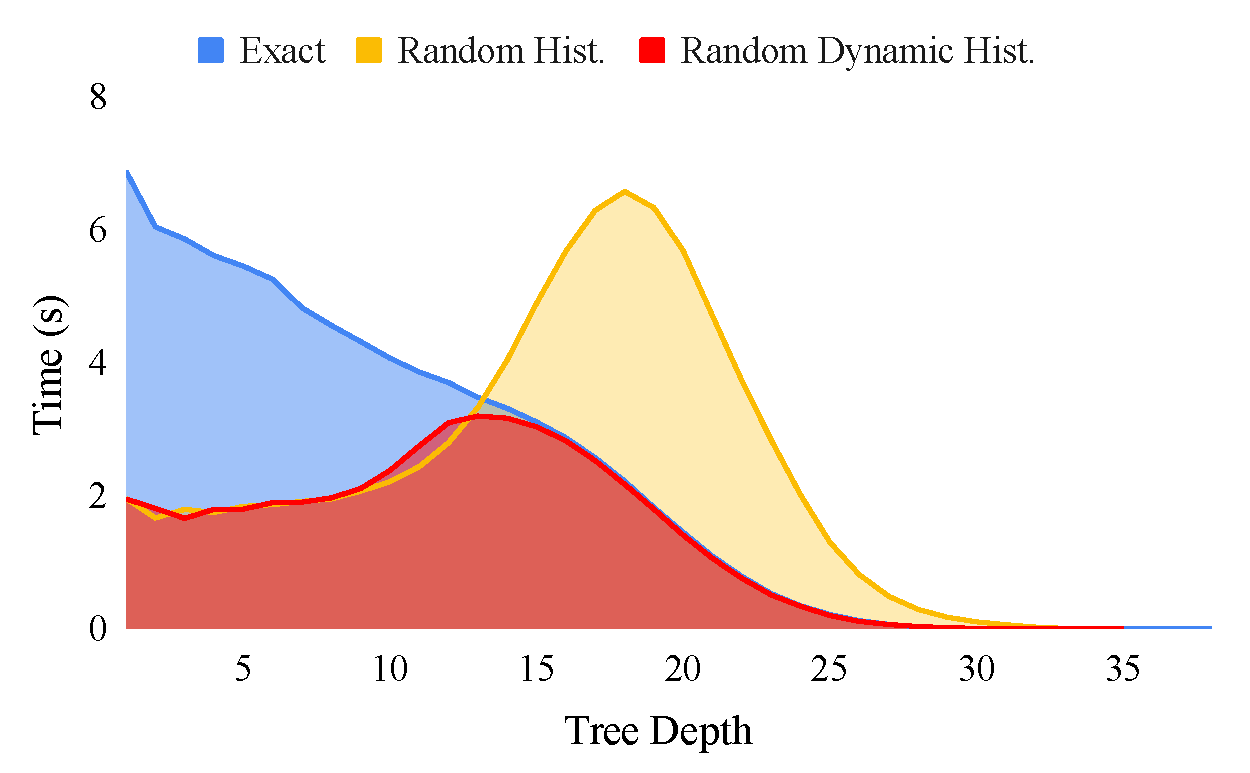
\includegraphics[width=0.478\textwidth]{figures/appendix/Scalar-Dynamic-HIGGS.pdf}

    \caption{Training runtime by tree depth on a dataset with 1M samples 4096 features between \texttt{std::sort} and scalar Random Hist. Exact was reduced by 2-3$\times$ with the advent of Highway.}

%RB NO -- this kind of interpretation goes in the text.
    %Exact splitting has a clear disadvantage in runtime at higher levels, while histogramming is slower at mid-depth. This is because sorting time rises with the number of active samples, while histogram time tracks the number of active nodes.}
    \label{fig:per-depth-dynamic}
    \Description{Area chart showing the runtime of Exact (sorting-based) splitting and Histogramming methods, at specific tree depths}
\end{figure}

Highway VQSort changes this picture. It trains $2.2\times$ faster than \texttt{std::sort} and, unlike \texttt{std::sort}, it beats the scalar histogram at every depth, including the root node that holds every sample (Figure~\ref{fig:dynamic-motivation-nodetrain}). Dynamic over the scalar histogram therefore no longer wins in any regime: it is $1.45\times$ slower than Highway Exact over the whole tree. Recovering the histogram's advantage requires the vectorized histogram filling of the main text, which is why every speedup in this paper is measured against Highway Exact rather than \texttt{std::sort}.

\subsection{YDF Pull Request Contributions}
\label{app:pull-requests}

\textit{Due to anonymity concerns with exact Pull-request numbers and titles, we only provide a summary below.}

This project has resulted in numerous improvements to the YDF library, contributed as pull requests:

\begin{itemize}
    \item \textbf{Candidate-attribute sampling.} The eager per-node shuffle of all attributes is replaced by a lazy prefix Fisher--Yates shuffle that only draws the few positions actually tested, and is up to 75\% faster on high-dimensional data.
    \item \textbf{Projection-evaluator caching.} We replaced an $O(F)$ object re-initialization with a cached and reused object per thread. Up to 3$\times$ faster on high-dimensional data.
    \item \textbf{Random-histogram split search.} Invariant code hoisted out of the candidate-threshold scan - up to 30\% for sparse oblique speedup.
    \item \textbf{Vectorized bin generation.} \texttt{std::sort} is replaced by Highway VQSort in generating histogram bins; up to 15\%.
    \item \textbf{Histogram split search for oblique forests.} Adds the histogram (approximate) split finder to the sparse-oblique path, which previously supported only exact splits.
    \item \textbf{Equal-width binning.} Samples are assigned to equal-width bins with $O(1)$ arithmetic instead of a binary search over the bin boundaries.
    \item \textbf{Projection sampling.} The per-feature uniform draws that build each sparse projection are replaced by one Binomial draw for the number of non-zeros plus Floyd's sampler for their positions, reducing the cost from linear in the number of features to linear in the number of non-zeros (proof below).
\end{itemize}

\paragraph{Floyd's projection sampling.}
Originally, random sampling to build the projection matrix was a computational bottleneck for SO-YDF. This component comprised 80\% of the runtime, with the math-heavy parts of the code taking <20\%. The previous design assumed small $d$ and was inefficient for wide data.

Existing code calls Unif(0,1) over the projection matrix to create a mask, then populates this mask with weights. However, this requires $\Theta(np)$ calls to {\tt Unif($\cdot$)}, or $p$ calls per each projection, across $n$ projections. We show this can be substituted with a single call to Binomial($np, n\frac{k}{p}$), cutting runtime by 33\% for our settings, proportional to $\Theta(np)$.

Using a variant of an algorithm from Floyd~\cite{10.1145/30401.315746}, we form the projection matrix as follows:

\begin{lstlisting}[language=c++]
projection_density = k/p;
for projection in projections:  // O(n)
    for feature in features:    // O(p)
        if (Unif01(.) < projection_density) {...}
\end{lstlisting}

% Proof commented out for the submission (kept for the final version).
% Let $z^n$ denote the actual number of successes from running this algorithm, i.e. the number of times the inner loop's \texttt{if} condition evaluates to \texttt{True}. We need to show $z^n \sim \text{Binomial}(np,n\frac{k}{p})$:
%
% \begin{proof}
%
% \begin{enumerate}
%     \item The probability of one true evaluation (success) of \texttt{if (Unif01(.) < projection\_density)} $\sim \text{Bernoulli}(\frac{k}{p})$ since \texttt{projection\_density} $=\frac{k}{p}$, and a success only occurs when a Unif(0,1) sample is $< \frac{k}{p}$.
%     \item Let $z^i$ denote the number of successes for each projection, where $i\in [0,n-1]$. $z_i \sim \text{Binomial}(p,\frac{k}{p})$ since by definition, a Binomial($1,\frac{k}{p})=\text{Bernoulli}(\frac{k}{p})$, and by the additive property of the Binomial, $\sum_p \text{Binomial}(1,\frac{k}{p})=\text{Binomial}(p,k)$.
%     \item The same property extends to $z^n=\sum_n z_i=\text{Binomial}(np,nk)$.
% \end{enumerate}
%
% \end{proof}

% This reduces runtime by 30\% for target input parameters. The benefit is linear with the number of projections.
%We PR-ed this function into the YDF repo (PR \#199 - \textit{beware breaking anonymity}).

\end{document}
